% Aliveness: Principles of Telic Systems
% Elias Kunnas, 2025

% Preamble for The Four Axiomatic Dilemmas
% Professional book typesetting with XeLaTeX

\documentclass[11pt,twoside,openright]{book}

% ============================================================================
% PAGE GEOMETRY
% ============================================================================
\usepackage[
    paperwidth=6in,
    paperheight=9in,
    top=0.75in,
    bottom=0.75in,
    inner=0.85in,  % Larger margin for binding
    outer=0.6in,
    headheight=24pt,  % Increased for fancy headers
    includeheadfoot
]{geometry}

% ============================================================================
% FONTS (XeLaTeX)
% ============================================================================
\usepackage{fontspec}

% Professional fonts for optimal readability
% Install with: brew tap homebrew/cask-fonts && brew install font-libertinus
% Fallback to Times New Roman if Libertinus not available
\IfFontExistsTF{Libertinus Serif}{
    \setmainfont{Libertinus Serif}[
        Ligatures=TeX,
        Numbers=OldStyle,
        Scale=1.0
    ]
    \setsansfont{Libertinus Sans}
    \setmonofont{Libertinus Mono}[Scale=0.9]
}{
    % Fallback to system fonts
    \setmainfont{Times New Roman}[Ligatures=TeX]
    \setsansfont{Helvetica}
    \setmonofont{Courier}[Scale=0.9]
}

% ============================================================================
% TYPOGRAPHY
% ============================================================================
\usepackage{microtype}       % Better typography
\usepackage{setspace}        % Line spacing control
\setstretch{1.15}            % 1.15 line spacing

% Paragraph formatting
\setlength{\parindent}{1em}
\setlength{\parskip}{0pt}

% Prevent overfull hboxes
\sloppy
\hyphenpenalty=5000
\tolerance=1000

% ============================================================================
% MATH (must load before cleveref)
% ============================================================================
\usepackage{amsmath}
\usepackage{amssymb}

% ============================================================================
% CROSS-REFERENCES AND HYPERLINKS
% ============================================================================
\usepackage{hyperref}
\hypersetup{
    colorlinks=true,
    linkcolor=blue,
    urlcolor=blue,
    citecolor=blue,
    bookmarksdepth=2,
    pdfauthor={Elias Kunnas},
    pdftitle={The Four Axiomatic Dilemmas},
    pdfsubject={Principles of Telic Systems},
    pdfkeywords={Aliveness, Wonder, SORT Framework, Civilization, AI Alignment, Human alignment, Telic systems}
}

% Enhanced cross-referencing (must come after hyperref)
\usepackage{cleveref}

% Configure cleveref labels
\crefname{section}{Section}{Sections}
\crefname{subsection}{Section}{Sections}
\crefname{subsubsection}{Section}{Sections}
\crefname{chapter}{Chapter}{Chapters}
\crefname{part}{Part}{Parts}
\crefname{equation}{Equation}{Equations}
\crefname{figure}{Figure}{Figures}
\crefname{table}{Table}{Tables}
\crefname{appendix}{Appendix}{Appendices}

% Note: After \appendix command, chapters become appendices
% Use \appendixname to reference them as "Appendix 1" etc.

% ============================================================================
% TABLE OF CONTENTS
% ============================================================================
\setcounter{tocdepth}{2}     % Show sections in TOC (Part=0, Chapter=1, Section=2)
\setcounter{secnumdepth}{3}  % Number subsubsections (keeps numbering in text)

% Fix appendix section numbering to show A.1, B.1, etc.
\makeatletter
\@addtoreset{section}{chapter}     % Reset section counter for each chapter
\@addtoreset{subsection}{chapter}  % Reset subsection counter for each chapter (appendices use subsections directly)
\makeatother

% ============================================================================
% HEADERS AND FOOTERS
% ============================================================================
\usepackage{fancyhdr}
\pagestyle{fancy}
\fancyhf{}  % Clear all headers/footers

% Enhanced headers: Part context on left, section on right
\fancyhead[LE]{\small\itshape\nouppercase{\partname\ \thepart\ |\ \leftmark}}
\fancyhead[RO]{\small\itshape\nouppercase{\rightmark}}

% Page numbers
\fancyfoot[LE,RO]{\small\thepage}

% Plain style for chapter opening pages
\fancypagestyle{plain}{
    \fancyhf{}
    \fancyfoot[C]{\small\thepage}
    \renewcommand{\headrulewidth}{0pt}
}

% *** FIX STARTS HERE ***
\usepackage{iftex} % Add this package to detect the engine

% Define dummy commands FIRST for Pandoc (before the main definitions)
\ifdefined\pandocVersion
    % Pandoc is running - define no-op commands early
    \providecommand{\startNarrativeChapter}{}
    \providecommand{\stopNarrativeChapter}{}
    \providecommand{\setDefaultNumbering}{}
    \providecommand{\setNarrativeNumbering}{}
\fi

% Check if we're being processed by Pandoc
\ifdefined\pandocVersion
    % Pandoc is running - skip all titlesec commands
\else
    % XeLaTeX or other processor - include titlesec
    % ============================================================================
    % CHAPTER AND SECTION FORMATTING
    % ============================================================================
    \usepackage{titlesec}

    % Part formatting (for PART I, II, III, etc.)
    \titleformat{\part}[display]
        {\centering\Huge\bfseries}
        {\MakeUppercase{\partname} \thepart}
        {20pt}
        {\Huge}

    % Chapter formatting
    \titleformat{\chapter}[display]
        {\normalfont\huge\bfseries}
        {\chaptertitlename\ \thechapter}
        {20pt}
        {\Huge}

    % Section formatting
    \titleformat{\section}
        {\normalfont\Large\bfseries}
        {\thesection}
        {1em}
        {}

    \titleformat{\subsection}
        {\normalfont\large\bfseries}
        {\thesubsection}
        {1em}
        {}

    \titleformat{\subsubsection}
        {\normalfont\normalsize\bfseries}
        {\thesubsubsection}
        {1em}
        {}

    % Improved spacing around sections
    \titlespacing{\section}{0pt}{2.5ex plus 1ex minus .2ex}{1.5ex plus .2ex}
    \titlespacing{\subsection}{0pt}{2ex plus 1ex minus .2ex}{1ex plus .2ex}
    \titlespacing{\subsubsection}{0pt}{1.5ex plus .5ex minus .2ex}{0.8ex plus .2ex}

    % ============================================================================
    % DUAL NUMBERING SYSTEM (Gnostic/Mythos Integration)
    % ============================================================================
    % This allows switching between default numeric and narrative Roman styles
    % without breaking cross-references or ToC, per the Gemini-Claude synthesis.

    % --- Default Numeric Style (Restored with \endNarrativeChapter) ---
    \providecommand{\setDefaultNumbering}{}
    \renewcommand{\setDefaultNumbering}{%
      \titleformat{\section}
        {\Large\bfseries}
        {\thesection} % Displays as chapter.section (e.g., "4.1")
        {1em}
        {}
      \titleformat{\subsection}
        {\large\bfseries}
        {\thesubsection} % Displays as chapter.section.subsection
        {1em}
        {}
    }

    % --- Narrative Numeric Style (Activated with \startNarrativeChapter) ---
    \providecommand{\setNarrativeNumbering}{}
    \renewcommand{\setNarrativeNumbering}{%
      \titleformat{\section}
        {\Large\bfseries}
        {\thechapter.\arabic{section}} % Displays as numeric (e.g., "13.1")
        {1em}
        {}
      \titleformat{\subsection}
        {\large\bfseries}
        {\thechapter.\arabic{section}.\arabic{subsection}} % ToC/ref friendly: 13.2.3
        {1em}
        {}
    }

    % Define the user-facing commands
    \providecommand{\startNarrativeChapter}{}
    \renewcommand{\startNarrativeChapter}{\setNarrativeNumbering}
    \providecommand{\stopNarrativeChapter}{}
    \renewcommand{\stopNarrativeChapter}{\setDefaultNumbering}

    % Ensure the default is set at the beginning of the document
    \AtBeginDocument{\setDefaultNumbering}
\fi
% *** FIX ENDS HERE ***


% ============================================================================
% SPECIAL ENVIRONMENTS
% ============================================================================

% For block quotes
\usepackage{mdframed}

% Block quotes - enhanced styling
\usepackage{csquotes}
\renewenvironment{quote}
  {\list{}{\leftmargin=2em\rightmargin=0em\itshape}\item[]}
  {\endlist}

% ============================================================================
% LISTS
% ============================================================================
\usepackage{enumitem}
\setlist{nosep, leftmargin=*, labelindent=\parindent, itemsep=0.5ex}

% ============================================================================
% EPISTEMIC STATUS BOXES
% ============================================================================
\usepackage{xcolor}
\usepackage{tcolorbox}
\tcbuselibrary{skins,breakable}

% Define epistemic status colors
\definecolor{epistemic-high}{RGB}{34, 139, 34}      % Forest green
\definecolor{epistemic-medium}{RGB}{255, 165, 0}    % Orange
\definecolor{epistemic-low}{RGB}{178, 34, 34}       % Firebrick red
\definecolor{epistemic-mixed}{RGB}{218, 165, 32}    % Goldenrod

% Epistemic status box environment
\newtcolorbox{epistemicbox}[2][]{
  colback=#2!5!white,
  colframe=#2!75!black,
  fonttitle=\bfseries,
  coltitle=black,
  title=Epistemic Status: #1,
  breakable,
  enhanced,
  attach boxed title to top left={yshift=-2mm, xshift=3mm},
  boxed title style={colback=#2!75!black, colframe=#2!75!black},
  top=3mm,
  bottom=3mm,
  left=3mm,
  right=3mm
}

% Convenience commands for each tier
\newcommand{\epistemichigh}[2]{%
  \begin{epistemicbox}[#1]{epistemic-high}
  #2
  \end{epistemicbox}
}

\newcommand{\epistemicmedium}[2]{%
  \begin{epistemicbox}[#1]{epistemic-medium}
  #2
  \end{epistemicbox}
}

\newcommand{\epistemiclow}[2]{%
  \begin{epistemicbox}[#1]{epistemic-low}
  #2
  \end{epistemicbox}
}

\newcommand{\epistemicmixed}[2]{%
  \begin{epistemicbox}[#1]{epistemic-mixed}
  #2
  \end{epistemicbox}
}

% SORT archetype notation - monospace for alignment
\newcommand{\sortarch}[4]{%
  \texttt{[S#1\,O#2\,R#3\,T#4]}%
}

% Pandoc-generated command for tight lists
\providecommand{\tightlist}{%
  \setlength{\itemsep}{0pt}\setlength{\parskip}{0pt}}

% ============================================================================
% TABLES AND FIGURES
% ============================================================================
\usepackage{booktabs}   % Professional tables
\usepackage{longtable}  % Multi-page tables
\usepackage{tabularx}   % Auto-width tables
\usepackage{multirow}   % Multi-row cells in tables
\usepackage{graphicx}   % For figures if needed
\usepackage{float}      % For H float option

% TikZ for high-quality diagrams
\usepackage{tikz}
\usetikzlibrary{arrows.meta,positioning,shapes.geometric,calc,decorations.pathreplacing}

% ============================================================================
% CODE BLOCKS (for ASCII art diagrams)
% ============================================================================
\usepackage{fancyvrb}
\usepackage{listings}

% Verbatim environment that doesn't break pages
\usepackage{needspace}

% Custom verbatim environment for diagrams
\DefineVerbatimEnvironment{diagram}{Verbatim}{
    fontsize=\small,
    fontfamily=tt,
    samepage=true
}

% ============================================================================
% ACRONYM MANAGEMENT
% ============================================================================
\usepackage{acronym}

% ============================================================================
% INDEX GENERATION
% ============================================================================
\usepackage{makeidx}
\makeindex

% ============================================================================
% MISCELLANEOUS
% ============================================================================

% Better spacing in arrays and matrices
\usepackage{array}

% For strikethrough text
\usepackage[normalem]{ulem}

% For colored text
\usepackage{xcolor}

% ============================================================================
% VISUAL HIERARCHY BOXES
% ============================================================================
\usepackage{tcolorbox}
\tcbuselibrary{skins,breakable}

% Key principle boxes (for major theorems and laws)
\newtcolorbox{keyprinciple}[1][]{
    colback=blue!5!white,
    colframe=blue!75!black,
    fonttitle=\bfseries,
    title=#1,
    breakable,
    enhanced jigsaw,
    before skip=10pt,
    after skip=10pt
}

% Definition boxes
\newtcolorbox{definition}[1][]{
    colback=gray!5!white,
    colframe=gray!75!black,
    fonttitle=\bfseries,
    title=Definition: #1,
    breakable,
    before skip=8pt,
    after skip=8pt
}

% Example boxes
\newtcolorbox{example}[1][]{
    colback=green!5!white,
    colframe=green!60!black,
    fonttitle=\bfseries,
    title=Example: #1,
    breakable,
    before skip=8pt,
    after skip=8pt
}

% Prevent widows and orphans
\widowpenalty=10000
\clubpenalty=10000
\raggedbottom

% Allow slightly more space between words if needed
\emergencystretch=3em

% ============================================================================
% CUSTOM COMMANDS
% ============================================================================

% Note: \Omega and \Psi are already defined by LaTeX as math symbols
% We don't need to redefine them - they work as-is in math mode
% Just use $\Omega$ and $\Psi$ directly in the text

% SORT notation
\newcommand{\SORT}{\textsc{sort}}
\newcommand{\SORTVC}{\textsc{sortvc}}
\newcommand{\pSORT}{\textsc{psort}}
\newcommand{\tSORT}{\textsc{tsort}}
\newcommand{\bioSORT}{\textsc{bio-sort}}

% States
\newcommand{\ALPHA}{\textsc{alpha}}
\newcommand{\BETA}{\textsc{beta}}
\newcommand{\GAMMA}{\textsc{gamma}}
\newcommand{\ENTROPIC}{\textsc{entropic}}

% Virtues (IFHS)
\newcommand{\IFHS}{\textsc{ifhs}}

% ============================================================================
% MATHEMATICAL NOTATION SHORTCUTS (Corrected & Harmonized)
% ============================================================================

% Use standard LaTeX math commands for consistency and portability.
% The \ensuremath command ensures they work correctly in and out of math mode.

% Civilizational Dynamics
\newcommand{\Omegac}{\ensuremath{\Omega}}           % State Coherence
\newcommand{\Alphac}{\ensuremath{\mathrm{A}}}       % Action Vector (Use Roman 'A' for distinction)
\newcommand{\Psic}{\ensuremath{\Psi}}               % Telic Potential (Soul)
\newcommand{\Nuc}{\ensuremath{\mathrm{N}}}          % Gnomic Potential (Mind) (Use Roman 'N')
\newcommand{\Kappac}{\ensuremath{\mathrm{K}}}       % Action Potential (Use Roman 'K')
\newcommand{\sigmac}{\ensuremath{\sigma_A}}         % Axiological variance

% Backward compatibility aliases (for standalone symbol use)
\newcommand{\Alpha}{\mathrm{A}}                     % Action Vector symbol (use in math mode)
\newcommand{\Nu}{\mathrm{N}}                        % Gnomic symbol (use in math mode)
\newcommand{\Kappa}{\mathrm{K}}                     % Action Potential symbol (use in math mode)

% Personal Dynamics (subscript p)
\newcommand{\Omegap}{\ensuremath{\Omega_p}}         % Personal Coherence
\newcommand{\Alphap}{\ensuremath{\mathrm{A}_p}}     % Personal Action

% Subscripted Omega Variants
\newcommand{\Omegainst}{\ensuremath{\Omega_{\text{institutional}}}}
\newcommand{\Omegakin}{\ensuremath{\Omega_{\text{kinetic}}}}
\newcommand{\Omegapop}{\ensuremath{\Omega_{\text{population}}}}

% Em dash
\newcommand{\emdash}{---}

% Status symbols (for tables and lists)
\newcommand{\pass}{\textcolor{green!70!black}{$\checkmark$}}
\newcommand{\fail}{\textcolor{red!70!black}{$\times$}}

% ============================================================================
% END PREAMBLE
% ============================================================================


\begin{document}

% ============================================================================
% FRONT MATTER
% ============================================================================
\frontmatter

% Title page
\begin{titlepage}
\centering
\vspace*{2cm}

{\Huge\bfseries Aliveness\par}
\vspace{0.5cm}
{\LARGE Principles of Telic Systems\par}
\vspace{2cm}
{\Large Elias Kunnas\par}
\vspace{1cm}
{\large October 2025\par}

\vfill

% Optional: Publisher or version info
% {\small Version 1.0\par}

\end{titlepage}

% Define acronyms early for TOC references
\acrodef{SORT}{Sovereignty-Organization-Reality-Telos Framework}
\acrodef{pSORT}{Personal SORT (individual-level application)}
\acrodef{tSORT}{Tribal SORT (sub-civilizational groups)}
\acrodef{SORTVC}{SORT plus Vitality and Constraint modifiers}
\acrodef{POSIWID}{Purpose Of a System Is What It Does}
\acrodef{IFHS}{Integrity, Fecundity, Harmony, Synergy (The Four Foundational Virtues)}

% Table of Contents
\tableofcontents
\cleardoublepage

% List of Acronyms
\chapter*{List of Acronyms}
\addcontentsline{toc}{chapter}{List of Acronyms}
\markboth{List of Acronyms}{List of Acronyms}

\begin{acronym}[POSIWID]  % Longest acronym for spacing
\acro{SORT}{Sovereignty-Organization-Reality-Telos Framework}
\acro{pSORT}{Personal SORT (individual-level application)}
\acro{tSORT}{Tribal SORT (sub-civilizational groups)}
\acro{SORTVC}{SORT plus Vitality and Constraint modifiers}
\acro{POSIWID}{Purpose Of a System Is What It Does}
\acro{IFHS}{Integrity, Fecundity, Harmony, Synergy (The Four Foundational/Constitutional Virtues)}
\end{acronym}

\cleardoublepage

% Framework at a Glance - One-page reference for the entire system
% ========================================
% FRAMEWORK AT A GLANCE
% Minimalist one-page cheat sheet inserted after TOC, before Foreword
% ========================================

\thispagestyle{empty}  % No page number
\begin{center}

\vspace*{0.5cm}

{\LARGE\textbf{Framework at a Glance}}

\vspace{0.5cm}

% ========================================
% I. THE SORT FRAMEWORK (4 Fundamental Axes)
% ========================================

{\large\textbf{I. The SORT Framework}}
\vspace{0.2cm}

\begin{small}
\begin{tabular}{@{}llll@{}}
\toprule
\textbf{Axis} & \textbf{Question} & \textbf{-1 Pole} & \textbf{+1 Pole} \\
\midrule
\textbf{S} (Sovereignty) & Who are we? & Individual & Collective \\
\textbf{O} (Organization) & How do we build? & Emergence & Design \\
\textbf{R} (Reality) & How do we know? & Mythos & Gnosis \\
\textbf{T} (Telos) & What do we seek? & Homeostasis & Metamorphosis \\
\bottomrule
\end{tabular}
\end{small}

\vspace{0.4cm}

% ========================================
% II. THE PHASE SPACE DIAGRAMS (Master Dynamics)
% ========================================

{\large\textbf{II. The Phase Space (Master Dynamics)}}
\vspace{0.2cm}

% Two diagrams side by side
\begin{minipage}[t]{0.48\textwidth}
\centering
{\small\textbf{Α-Ω (Pedagogical Simplification)}}
\vspace{0.1cm}

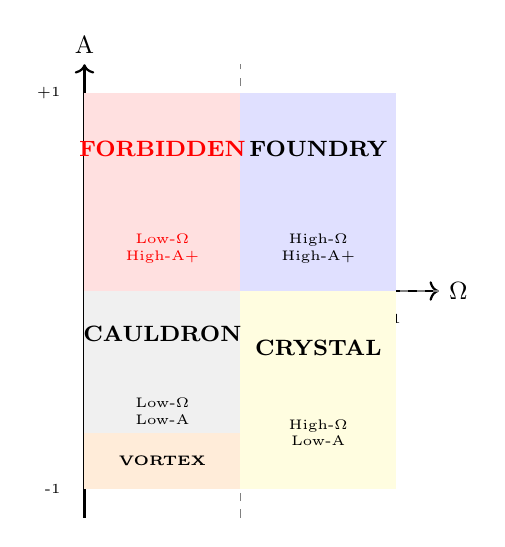
\begin{tikzpicture}[scale=1.8]
    % Axes
    \draw[->,thick] (0,0) -- (2.5,0) node[right,font=\small] {$\Omega$};
    \draw[->,thick] (0,-1.6) -- (0,1.6) node[above,font=\small] {$\Alpha$};

    % Ticks
    \node[below,font=\tiny] at (2.2,-0.1) {1};
    \node[left,font=\tiny] at (-0.1,1.4) {+1};
    \node[left,font=\tiny] at (-0.1,-1.4) {-1};

    % Quadrant boundaries
    \draw[gray,thin,dashed] (1.1,-1.6) -- (1.1,1.6);
    \draw[gray,thin,dashed] (0,0) -- (2.5,0);

    % Quadrant fills and labels (SMALLER TEXT)
    \fill[blue!12] (1.1,0) rectangle (2.2,1.4);
    \node[align=center,font=\footnotesize\bfseries] at (1.65, 1.0) {FOUNDRY};
    \node[align=center,font=\tiny] at (1.65, 0.3) {High-$\Omega$\\High-$\Alpha$+};

    \fill[red!12] (0,0) rectangle (1.1,1.4);
    \node[align=center,font=\footnotesize\bfseries,red] at (0.55, 1.0) {FORBIDDEN};
    \node[align=center,font=\tiny,red] at (0.55, 0.3) {Low-$\Omega$\\High-$\Alpha$+};

    \fill[yellow!12] (1.1,-1.4) rectangle (2.2,0);
    \node[align=center,font=\footnotesize\bfseries] at (1.65, -0.4) {CRYSTAL};
    \node[align=center,font=\tiny] at (1.65, -1.0) {High-$\Omega$\\Low-$\Alpha$};

    \fill[gray!12] (0,-1.4) rectangle (1.1,0);
    \node[align=center,font=\footnotesize\bfseries] at (0.55, -0.3) {CAULDRON};
    \node[align=center,font=\tiny] at (0.55, -0.85) {Low-$\Omega$\\Low-$\Alpha$};

    % Vortex sub-region
    \fill[orange!15] (0,-1.4) rectangle (1.1,-1.0);
    \node[align=center,font=\tiny\bfseries] at (0.55, -1.2) {VORTEX};
\end{tikzpicture}
\end{minipage}
\hfill
\begin{minipage}[t]{0.48\textwidth}
\centering
{\small\textbf{T-Ω (Causal Mechanics)}}
\vspace{0.1cm}

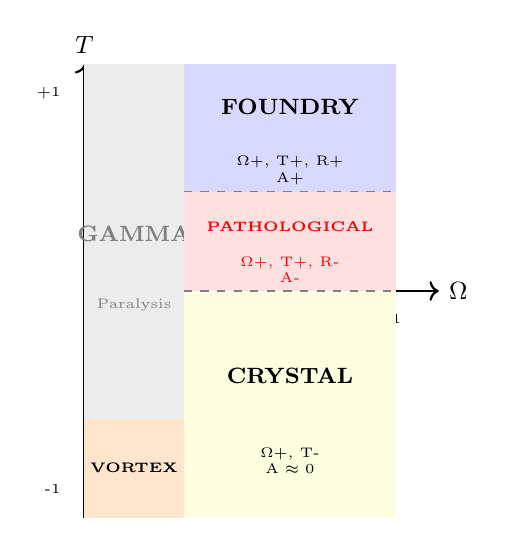
\begin{tikzpicture}[scale=1.8]
    % Axes
    \draw[->,thick] (0,0) -- (2.5,0) node[right,font=\small] {$\Omega$};
    \draw[->,thick] (0,-1.6) -- (0,1.6) node[above,font=\small] {$T$};

    % Ticks
    \node[below,font=\tiny] at (2.2,-0.1) {1};
    \node[left,font=\tiny] at (-0.1,1.4) {+1};
    \node[left,font=\tiny] at (-0.1,-1.4) {-1};

    % Iron Law threshold
    \draw[red,thick,dashed] (0.7,-1.6) -- (0.7,1.6);
    \node[red,font=\tiny,align=center,rotate=90] at (0.4,0) {Iron Law};

    % LEFT REGION: Low-Ω
    \fill[gray!15] (0,-1.6) rectangle (0.7,1.6);
    \node[align=center,font=\footnotesize\bfseries,gray] at (0.35,0.4) {GAMMA};
    \node[align=center,font=\tiny,gray] at (0.35,-0.1) {Paralysis};

    \fill[orange!20] (0,-1.6) rectangle (0.7,-0.9);
    \node[align=center,font=\tiny\bfseries] at (0.35,-1.25) {VORTEX};

    % Bottom-Right: High-Ω, T-
    \fill[yellow!12] (0.7,-1.6) rectangle (2.2,0);
    \node[align=center,font=\footnotesize\bfseries] at (1.45,-0.6) {CRYSTAL};
    \node[align=center,font=\tiny] at (1.45,-1.2) {$\Omega$+, T-\\$\Alpha \approx 0$};

    % Top-Right: Foundry (R+ upper, R- lower)
    \fill[blue!15] (0.7,0.7) rectangle (2.2,1.6);
    \node[align=center,font=\footnotesize\bfseries] at (1.45,1.3) {FOUNDRY};
    \node[align=center,font=\tiny] at (1.45,0.85) {$\Omega$+, T+, R+\\$\Alpha$+};

    \fill[red!12] (0.7,0) rectangle (2.2,0.7);
    \node[align=center,font=\tiny\bfseries,red] at (1.45,0.45) {PATHOLOGICAL};
    \node[align=center,font=\tiny,red] at (1.45,0.15) {$\Omega$+, T+, R-\\$\Alpha$-};

    % Divider
    \draw[gray,thin,dashed] (0.7,0) -- (2.2,0);
    \draw[gray,thin,dashed] (0.7,0.7) -- (2.2,0.7);
\end{tikzpicture}
\end{minipage}

\vspace{0.3cm}

\begin{small}
\textbf{$\Omega$ (Coherence):} Internal unity (0 = fragmented, 1 = unified) \quad
\textbf{$\Alpha$ (Action):} Net output (-1 = entropic, +1 = syntropic)

\textbf{Iron Law of Coherence (Theorem):} Low-Ω, High-Α+ is \textit{impossible}. Synergy is non-negotiable precondition for Syntropy. The Α-Ω diagram shows \textit{observed outputs}; T-Ω reveals \textit{causal mechanics}.
\end{small}

\vspace{0.4cm}

% ========================================
% III. THE FOUR VIRTUES (IFHS)
% ========================================

{\large\bfseries III. The Four Virtues (The Optimal Solution)}
\vspace{0.3cm}

\begin{small}
\begin{tabular}{@{} >{\bfseries}l >{\itshape}l p{9cm} @{}}
\toprule
Virtue & Solves & Definition \\
\midrule
Integrity (I) & R-Axis & The Gnostic pursuit of a truthful Mythos (Truth + Meaning). \\
\addlinespace
Fecundity (F) & T-Axis & The creation of stable conditions for new growth (Stability + Growth). \\
\addlinespace
Harmony (H) & O-Axis & The use of minimal Design to unleash maximal Emergence (Order + Freedom). \\
\addlinespace
Synergy (S) & S-Axis & An architecture where the whole is greater than the sum of its parts (Individual + Collective = superadditive value). \\
\bottomrule
\end{tabular}
\end{small}

\vspace{0.6cm}

% ========================================
% IV. THE 3-LAYER ARCHITECTURE
% ========================================

{\large\bfseries IV. The 3-Layer Architecture (The Engineered Form)}
\vspace{0.3cm}

\begin{small}
\begin{tabular}{@{} >{\bfseries}l >{\itshape}l p{8cm} @{}}
\toprule
Layer & Function & Core Axiological Mode \\
\midrule
Head & Direction (T+) & \textbf{Instrumental:} Gnostic, Metamorphic, Pragmatic \\
\addlinespace
Skeleton & Constraint (T-) & \textbf{Protocol:} Gnostic, Designed, Principled \\
\addlinespace
Heart & Continuity (T-) & \textbf{Integrative:} Mythopoetic, Emergent, Somatic \\
\bottomrule
\end{tabular}
\end{small}

\vspace{0.3cm}
\begin{small}
\textit{Holographic Principle: This scale-invariant architecture is the stable solution for cells, organisms, individuals, and civilizations.}
\end{small}

\end{center}

\cleardoublepage


% Foreword
\chapter*{Foreword}
\addcontentsline{toc}{chapter}{Foreword}
\markboth{Foreword}{Foreword}


\section*{The Axiological Wager}
\vspace{0.5em}

This book wagers that the rise and fall of civilizations, the alignment of artificial intelligence, and the flourishing of individual consciousness are not separate problems. They are scale-invariant manifestations of the same underlying physics.

Any intelligent system---whether human civilization, alien species, or artificial intelligence---faces three inescapable computational problems: the \textbf{Trinity of Tensions} (the Problem of the World, the Problem of Time, and the Problem of the Self). The solutions any system chooses within this constraint space determine its trajectory, its health, and its ultimate fate.

\vspace{0.5em}

Our civilization is lost---navigating a hurricane with a child's drawing of the ocean. The Left/Right compass has failed catastrophically. But this failure is our \textbf{case study}. The framework applies universally. The rise and fall of civilizations follows hard, computational principles---laws as ruthless as gravity.

The wager of this book is that these laws can be deciphered. What follows is a proposed V1.0 of that codification, offered for testing.

\needspace{10\baselineskip}
\section{\texorpdfstring{\textbf{The Convergence Thesis: Logical Convergence Across Scales}}{The Convergence Thesis: Logical Convergence Across Scales}}\label{convergence-thesis}

The framework's credibility rests on a testable claim about convergent validity.

Descending to first principles reveals four inescapable trade-offs any negentropic, goal-directed system must navigate: the Four Axiomatic Dilemmas (\Cref{part:source-code}). These generate the Trinity of Tensions that any intelligent system faces.

Analyzing what maximizes long-term flourishing of complex, conscious systems yields four necessary conditions: \textbf{Integrity, Fecundity, Harmony, Synergy} (IFHS).

\vspace{0.5em}

\textbf{The convergence thesis:} When this same first-principles analysis is applied independently to three distinct scales---

\begin{enumerate}
\item \textbf{Civilizational flourishing}: What axiological configuration maximizes Aliveness of human societies over deep time?

\item \textbf{AI alignment}: What principles are necessary (though not sufficient) for artificial intelligence to preserve and enhance complex conscious life?

\item \textbf{Individual integration}: What principles govern healthy development of a single conscious agent?
\end{enumerate}

---all three analyses converge on the same necessary conditions: IFHS.

\vspace{0.5em}

This convergence across radically different scales, derived from the same universal physics, provides evidence that the framework describes real computational geometry rather than cultural preference.

The framework's power comes from deriving the same answers from different starting points. This is either discovering real constraints on the space of viable intelligent systems, or it is discovering nothing at all.

\vspace{0.5em}

\textbf{Falsifiability:} If independent researchers applying rigorous analysis to these three problems arrive at fundamentally different optimal solutions---or if the framework's predictions fail systematically---the convergence thesis fails. Complete AI alignment analysis: \Cref{app:ai-alignment}.

\needspace{10\baselineskip}
\section{\texorpdfstring{\textbf{How to Read This Book: Two Epistemological Tiers}}{How to Read This Book: Two Epistemological Tiers}}\label{how-to-read-this-book}

This framework presents two distinct epistemological tiers requiring different levels of scrutiny.

\textbf{Tier 1 --- Core Canon:} Claims derived from first principles of thermodynamics, information theory, and computation: the Four Axiomatic Dilemmas, the Trinity, and the Iron Law of Coherence. Judge these on their logical rigor and derivation from established physical laws.

\textbf{Tier 2 --- Research Extensions:} Synthetic observations from history (Four Horsemen of Decay, SORT signatures), untested engineering blueprints (Athenian Commonwealth, Unmasking Protocol), and theoretical predictions requiring validation. These are falsifiable hypotheses whose validity must be determined through empirical testing and real-world results.

Distinguishing between these tiers is essential. A Tier 2 claim (SORT score for Rome, efficacy of Liquid Meritocracy) should not be evaluated with the same criteria as a Tier 1 claim (thermodynamic necessity of the Boundary Dilemma). Conflating these categories obscures the actual falsification targets.

\needspace{10\baselineskip}
\section{\texorpdfstring{\textbf{A Note on Discovery \& Methodology}}{A Note on Discovery \& Methodology}}\label{a-note-on-discovery-methodology}

Before proceeding, you must understand how this framework was created.

\needspace{8\baselineskip}
\subsection{\texorpdfstring{\textbf{On AI-Mediated Synthesis}}{On AI-Mediated Synthesis}}\label{ai-mediated-synthesis}

Both the theoretical insights and the text were generated through sustained \textbf{AI-mediated synthesis}: approximately two months of iterative exploration across domains (history, physics, psychology, institutions), followed by focused formalization into the structured V1.0 text you are reading.

\vspace{0.5em}

\textbf{The Process:} AI-mediated pattern recognition across compressed historical knowledge via iterative, adversarial questioning (\textbf{Dialectical Tree Search}, \Cref{app:methodology}). I provided direction, frame selection, judgment, synthesis. The AI functioned as cognitive prosthetic---extending working memory, enabling rapid cross-domain synthesis. The result is human judgment integrated with AI synthesis: differentiated functions producing outcomes neither achieves alone.

\vspace{0.5em}

\textbf{What This Is:} Theoretical synthesis from pattern recognition across domains, analogous to Darwin synthesizing observations into unified evolutionary theory, not laboratory measurement of controlled variables. SORT scores are informed theoretical estimates, not rigorous quantitative measurements from controlled studies. The framework generates testable predictions (Virus Crucible, SORT correlations, Iron Law) alongside theoretical synthesis (Four Axiomatic Dilemmas from thermodynamics).

\vspace{0.5em}

\textbf{Epistemic Status:} Framework validity rests on explanatory power, internal consistency, and empirical validation. Confidence defined by Epistemological Tiers (\Cref{app:lexicon}). This is V1.0 theoretical framework offered for testing, falsification, and refinement.

Complete methodology: \Cref{app:methodology}.

\needspace{10\baselineskip}
\section{\texorpdfstring{\textbf{The Meta-axiological Foundation}}{The Meta-axiological Foundation}}\label{the-meta-axiological-foundation}

This work is not value-neutral. It rests on a prior commitment to \textbf{Aliveness} as the terminal value---the measure by which civilizations should be judged.

I define Aliveness as: \textbf{The capacity of a system to generate and sustain complexity, consciousness, and creative possibility over deep time.}

IF you value continued human existence, civilizational flourishing across generations, purpose and meaning, future possibilities over present comfort, and the preservation of human consciousness in a post-AGI world---THEN this framework offers superior diagnostic and engineering tools as an instrumental strategy.

If you believe maximal present comfort, elimination of struggle, or radical equality of outcome are the highest goods, different conclusions may follow.

I believe Aliveness is the only coherent terminal value for a civilization that wishes to persist. But this is a \textbf{premise}, not a proven fact. Everything that follows is conditional on accepting it.

The rest of this book can be read as: ``Given Aliveness as the goal, here is a proposed physics of how civilizations and intelligent systems succeed or fail in achieving it.''

\needspace{10\baselineskip}
\section{\texorpdfstring{\textbf{What This Book Is---and Is Not}}{What This Book Is---and Is Not}}\label{what-this-book-isand-is-not}

This is an engineering manual: diagnostic tools, testable predictions, and blueprints derived from first principles. It replaces arbitrary political dimensions with physics-derived axes grounded in thermodynamic necessity.

It is optimized for high-agency builders who view civilization as a system to debug and improve. If you seek testable frameworks for diagnosing and engineering telic systems at any scale: continue.

\needspace{10\baselineskip}
\section{\texorpdfstring{\textbf{The Transformation Arc}}{The Transformation Arc}}\label{the-transformation-arc}

The transformation: Blind Observer → Diagnostic Engineer → Integrated Human. This occurs holographically across scales. The Re-Founding of civilization begins with Re-Founding of self.

\vspace{0.5em}

\textbf{Part I (Diagnosis):} Install SORT framework, diagnose any polity's axiological DNA.

\textbf{Part II (Autopsy):} Apply framework to modern West. Understand the American Chimera, Hospice Axiology, and engines of decay.

\textbf{Part III (Source Code):} Descend to Four Axiomatic Dilemmas and Trinity of Tensions---the universal physics any intelligent system must navigate. Validate convergence thesis: civilization + AI + individual independently → IFHS. Virus Crucible demonstrates sharp falsifiability.

\textbf{Part IV (Blueprint):} Derive IFHS from first principles. Architect the Athenian Commonwealth as vehicle enabling Syntropic Republic. Exit with complete engineering blueprint.

\textbf{Part V (Integrated Human):} Apply same physics to personal scale via pSORT and Unmasking protocol. If the framework cannot apply to individual consciousness with the same rigor as civilizational analysis, its claim to universality fails.

\vspace{0.5em}

By the end, you will diagnose civilizations using SORT, explain rise and fall from first principles, understand why civilization-building and AI alignment converge on the same physics, design institutions that resist decay, apply the framework to your own psyche, and choose your path in the Re-Founding work.

\needspace{10\baselineskip}
\section{\texorpdfstring{\textbf{On the Division of Intellectual Labor}}{On the Division of Intellectual Labor}}\label{on-the-division-of-intellectual-labor}

I am a \textbf{synthesizer}, not a \textbf{validator}. This is 0-to-1 pattern recognition (connected history, neuroscience, game theory, biology, AI alignment), not 1-to-N empirical validation. Both roles necessary.

\textbf{The invitation:} Version 1.0 of generative hypothesis. Validation, falsification, refinement is distributed work requiring your contribution.

\textbf{Validators}: Test predictions (Virus Crucible, SORT correlations), find counterexamples, challenge isomorphism claims. \textbf{Builders}: Implement blueprints, test principles, iterate. \textbf{Theorists}: Formalize Trinity mathematically, extend to alien intelligences, build superior frameworks.

\textbf{Success metric:} This work succeeds if it bootstraps serious research into the physics of telic systems—a tractable, neglected, and existentially important domain. Better comprehensive synthesis partially wrong than safe incrementalism precisely irrelevant.

\vspace{0.5em}

The highest form of success: this V1.0 framework gets superseded by a superior V2.0 that a thriving research community builds. The goal is not to be right. The goal is to make this domain no longer neglected.


\needspace{10\baselineskip}
\section{\texorpdfstring{\textbf{The Engineer's Dilemma}}{The Engineer's Dilemma}}\label{the-engineers-dilemma}

You are building the future---new technologies, companies, frontiers. But you face a dilemma: launching rockets from a rotting platform. The civilization that produced you now wars against the principles of competence, merit, and striving that make your work possible.

Your projects cannot achieve escape velocity chained to a dying civilization. Building a starship is trivial compared to ensuring a civilization capable of launching it. \Cref{part:blueprint} addresses the external platform; \Cref{part:integrated-human} applies the same physics to personal integration.

\textbf{This is the missing half of your engineering problem.} Apply your engineer's mind to the civilizational machine itself. Move from engineering things to engineering worlds.

Our decline follows principles we can understand. Any system whose principles we grasp, we can engineer.

The framework predicts that the physics governing civilizational health is the same physics governing AI alignment---both questions reduce to optimization within the Trinity constraint space. If this hypothesis holds, both converge on identical necessary conditions (IFHS), though AI alignment requires additional sufficient conditions beyond the scope of this work (detailed treatment in \Cref{app:ai-alignment}).

The wager: sufficient understanding can catalyze deliberate Re-Founding. The Foundry can be re-ignited---not just for human civilizations, but as foundation for aligned intelligence at any scale.

The work is immense. The stakes are existential. The tools are in your hands.

Let us begin.

\vspace{0.5em}

What follows is systematic engineering. The diagnosis begins.


% ============================================================================
% MAIN MATTER
% ============================================================================
\mainmatter

% ============================================================================
% PART I: THE DIAGNOSIS
% ============================================================================
\part{The Diagnosis: The Broken Compass}
\label{part:diagnosis}

\chapter{The Broken Compass}
\label{ch:broken-compass}


The primary models used to understand political reality are failed pieces of engineering: the \textbf{one-dimensional spectrum of Left vs.~Right} and the \textbf{two-dimensional Political Compass} (Economic × Social axes).

They generate incorrect outputs. They make reality illegible.

For over two centuries, these low-dimensional coordinate systems have been the master frameworks for political thought, forcing complex multi-dimensional questions into binary or quadrant-based choices.

Both models fail. The 1D line fails on three levels. The 2D plane fails on the same three levels and adds a fourth.

\needspace{10\baselineskip}
\section{\texorpdfstring{\textbf{Proof by Origin: The Accident of History}}{Proof by Origin: The Accident of History}}\label{proof-by-origin}

The Left/Right spectrum was not derived from first principles---it was \textbf{inherited from a seating chart}.

In 1789, French National Assembly monarchists sat right, revolutionaries left. This snapshot of one conflict---king versus republic---was universalized across all political thought for two centuries.

No engineer would design a navigation system this way. Coordinate systems should derive from the \textbf{structure of the territory}, not from where people sat in a room 235 years ago.

The model was inherited, not engineered. This is the first proof of failure.

\needspace{10\baselineskip}
\section{\texorpdfstring{\textbf{Proof by Incoherence: The Collapse of Categories}}{Proof by Incoherence: The Collapse of Categories}}\label{proof-by-incoherence}

A failed model produces incoherent categories. When members of the same ``side'' hold contradictory positions on fundamental questions, the category has collapsed.

\needspace{8\baselineskip}
\subsection{\texorpdfstring{\textbf{The Right-Wing Audit}}{The Right-Wing Audit}}\label{right-wing-audit}

What principle unifies the American ``Right''?

\vspace{0.5em}

\textbf{Member A: Christian Social Conservative}
\begin{itemize}
\item Seeks strong communities, traditional families, embedded identity
\item Grounds truth in sacred texts and ancestral wisdom
\item Axiological signature: Collective sovereignty, Mythopoetic epistemology, Homeostatic purpose (preservation over growth)
\end{itemize}

\textbf{Member B: Libertarian Techno-Optimist}
\begin{itemize}
\item Seeks atomized individualism, creative destruction, perpetual disruption
\item Grounds truth in empirical data and falsifiable experiment
\item Axiological signature: Individual sovereignty, Gnostic epistemology, Metamorphic purpose (transformation through growth)
\end{itemize}

\vspace{0.5em}

These are \textbf{opposed axiologies} sharing a tribal label. One seeks preservation of traditional order, the other transformation through individual agency. One trusts inherited stories, the other empirical data. One values collective cohesion, the other personal autonomy.

They agree on policy outputs (lower taxes, less regulation) but represent fundamentally different answers to the deepest questions: Who are we? What do we seek? How do we know what's real?

The category ``Right'' collapses them into the same coordinate.

\needspace{8\baselineskip}
\subsection{\texorpdfstring{\textbf{The Left-Wing Audit}}{The Left-Wing Audit}}\label{left-wing-audit}

What principle unifies the American ``Left''?

\vspace{0.5em}

\textbf{Member A: Union Socialist}
\begin{itemize}
\item Believes in class power and economic solidarity
\item Views society through material lens of class struggle
\item Axiological signature: Collective sovereignty, Designed order (top-down control)
\end{itemize}

\textbf{Member B: Postmodern Academic}
\begin{itemize}
\item Calls ``class'' an oppressive meta-narrative
\item Celebrates fluid identity and deconstructed categories
\item Axiological signature: Individual sovereignty (identity over group), Mythopoetic epistemology
\end{itemize}

\vspace{0.5em}

One demands collective solidarity through class identity. The other calls all collective categories oppressive constructs.

The labels no longer describe beliefs. They describe tribes—coalitions of convenience, not coherent worldviews.

When members of the same ``side'' hold contradictory positions on fundamental questions---individual versus collective sovereignty, truth through data versus truth through narrative, preservation versus transformation---the category has collapsed.

This is the second proof of failure.

\needspace{10\baselineskip}
\section{\texorpdfstring{\textbf{Proof by Insufficiency: The Orthogonality Problem}}{Proof by Insufficiency: The Orthogonality Problem}}\label{proof-by-insufficiency}

The most damning failure applies to both 1D and 2D models: the questions that will determine civilizational survival in the next century cannot be plotted on either map.

\needspace{8\baselineskip}
\subsection{\texorpdfstring{\textbf{Case A: AI Alignment}}{Case A: AI Alignment}}\label{case-ai-alignment}

Where does ``preventing human extinction by superintelligent AI'' fall on the Left/Right spectrum?

Is it ``conservative'' or ``liberal''? ``Progressive'' or ``reactionary''? ``Authoritarian'' or ``Libertarian''?

The question is incoherent in this vocabulary. The issue is orthogonal to the axis.

Some on the Right embrace AI development as technological progress and individual freedom. Others reject it as violation of natural order and divine creation.

Some on the Left support AI as tool for human enhancement and solving collective problems. Others oppose it as capitalist automation threatening workers.

How to build machine intelligence that doesn't destroy its creators cuts across all existing tribal lines. The axes cannot encode it.

\needspace{8\baselineskip}
\subsection{\texorpdfstring{\textbf{Case B: Civilizational Growth Strategy}}{Case B: Civilizational Growth Strategy}}\label{case-growth-strategy}

The choice between two fundamentally different strategies for civilizational existence:

\vspace{0.5em}

\textbf{Strategy A: High-Growth/High-Risk}
\begin{itemize}
\item Maximize innovation, accept disruption
\item Optimize for future possibility over present comfort
\item Embrace creative destruction
\item Demographics: High fertility, youth orientation
\item Economics: Risk-tolerant capital, entrepreneurship
\item Culture: Ambition, striving, transcendence
\end{itemize}

\textbf{Strategy B: Low-Growth/Low-Risk}
\begin{itemize}
\item Minimize change, preserve stability
\item Optimize for present sustainability over future expansion
\item Resist disruption
\item Demographics: Low fertility, aging orientation
\item Economics: Safety-seeking capital, regulation
\item Culture: Comfort, safety, maintenance
\end{itemize}

\vspace{0.5em}

This choice determines demographic policy, economic strategy, technological development, immigration policy, and education systems. It is perhaps the most consequential question a civilization faces.

Yet it is \textbf{completely orthogonal} to the Left/Right spectrum and the Economic/Social plane.

You can have a left-wing high-growth society (Maoist China's Great Leap Forward) or a left-wing low-growth society (modern Western Europe). You can have a right-wing high-growth society (Gilded Age America) or a right-wing low-growth society (agrarian conservatism).

The growth strategy is an independent dimension of civilizational choice.

\vspace{0.5em}

The model is \textbf{dimensionally insufficient}. The territory of civilizational reality has at least four orthogonal dimensions. Our maps have one or two.

We are navigating a hypercube with a line or a plane.

This is the third proof of failure.

\needspace{10\baselineskip}
\section{\texorpdfstring{\textbf{The Two-Dimensional Cage: A More Sophisticated Failure}}{The Two-Dimensional Cage: A More Sophisticated Failure}}\label{the-two-dimensional-cage}

The Political Compass uses two dimensions---economic policy (Left/Right) crossed with social policy (Authoritarian/Libertarian).

This 2D model is indeed an improvement over the single axis. Like a flat map of Earth is an improvement over a single longitude line.

But it remains a fundamentally flawed piece of engineering. It fails for the same reasons as its predecessor and introduces new pathologies.

\needspace{8\baselineskip}
\subsection{\texorpdfstring{\textbf{The Same Proofs Still Apply}}{The Same Proofs Still Apply}}\label{same-proofs-apply}

The 2D model fails on the same three levels:

The axes remain \textbf{arbitrary}---not derived from first principles but from descriptive categorization of existing positions, patching the 1789 accident with a second dimension.

Categories remain \textbf{incoherent}---a Gnostic techno-optimist seeking transformation through technology and a traditionalist homesteader seeking preservation through ancestral wisdom share the same ``Libertarian-Right'' quadrant despite fundamentally opposed axiologies.

Fundamental choices remain \textbf{orthogonal} to the plane---the choice between Metamorphic growth versus Homeostatic stability, between Gnostic epistemology versus Mythopoetic epistemology, between future possibility and present sustainability. The territory has at least four orthogonal dimensions. The 2D map still has only two.

\needspace{8\baselineskip}
\subsection{\texorpdfstring{\textbf{The New Failure: False Independence}}{The New Failure: False Independence}}\label{false-independence}

The 2D model introduces a new, more subtle error: it assumes a polity can sustainably occupy \textbf{any point on its grid}.

It treats its axes as not only geometrically independent (which they are---you can define them orthogonally) but also \textbf{dynamically independent}---that any combination of economic and social policy is equally viable and sustainable.

The physics of civilizational dynamics reveals this is false.

\vspace{0.5em}

While axes can be designed to be \textbf{geometrically orthogonal}---representing distinct, independent questions---the laws of physics and game theory create powerful \textbf{dynamical entanglements} between them.

A civilization's choice on one axis creates energetic gradients and selective pressures that constrain positions on other axes.

\vspace{0.5em}

\textbf{Concrete Example:}

A civilization pursuing an ambitious Great Work like conquering a continent or colonizing space faces immense coordination demands: resource mobilization at civilizational scale, long-term strategic planning across generations, sustained focus despite short-term costs.

Purely emergent, bottom-up institutions cannot provide this. Spontaneous order excels at adaptation and wealth creation through distributed experimentation, but it cannot design and execute a Manhattan Project or an Apollo Program.

History confirms this: successful Metamorphic empires---Rome, Britain during imperial expansion, the United States during westward expansion---all developed significant top-down designed institutions. Legions and bureaucracies. Legal codes and administrative structures.

The choice of Metamorphic purpose creates selective pressure toward designed coordination mechanisms.

\vspace{0.5em}

The axes remain orthogonal \textbf{in principle}---you can ask the questions independently. But physics creates \textbf{corridors of viability in practice}. Certain combinations are sustainable, others unstable, some theoretically elegant but practically fragile.

The 2D compass, lacking physical grounding, presents a menu of choices as if all are equally viable. It does not reveal which combinations the universe permits.

\vspace{0.5em}

This is the fourth proof of failure---unique to the 2D model.

\needspace{10\baselineskip}
\section{\texorpdfstring{\textbf{The American Paradox: A Concrete Demonstration}}{The American Paradox: A Concrete Demonstration}}\label{the-american-paradox}

Modern America simultaneously exhibits anarchic chaos and tyrannical control.

Certain communities experience zero law enforcement, institutional collapse, open disorder. Others experience zealous prosecution for minor violations, oppressive bureaucratic control. This is selective enforcement \textbf{within the same jurisdictions}.

Standard Left/Right analysis diagnoses this as polarization between big government and small government, requiring compromise along the existing axis.

This analysis fails immediately. The paradox is not ``too much government versus too little government.'' It is \textbf{selective enforcement of order itself}---both anarchy and tyranny simultaneously, selectively applied to different groups based on axiological alignment.

\vspace{0.5em}

Explaining this phenomenon requires mapping:

\begin{itemize}
\item \textbf{Who} has power? What is the sovereignty distribution across different factions?
\item \textbf{How} coherently organized? What coordination mechanisms do power holders employ?
\item \textbf{What} epistemology guides enforcement decisions? What criteria determine ``truth'' and ``harm''?
\item \textbf{What} purpose does selective order serve? What is the telos of the power-holding faction?
\end{itemize}

Neither the one-dimensional spectrum nor the two-dimensional plane can encode this information. The questions are orthogonal to the axes provided.

\vspace{0.5em}

The broken compass cannot describe what you are experiencing, let alone explain or predict it.

The model has failed.

\needspace{10\baselineskip}
\section{\texorpdfstring{\textbf{The Verdict}}{The Verdict}}\label{the-verdict}

Failed models generate active pathology. Binary and quadrant frameworks force endless conflict over arbitrary lines while multi-dimensional dangers---demographic collapse, institutional decay, technological disruption, AI alignment challenges---gather unopposed.

The political class has no incentive to provide a better map. Their power depends on maintaining binary conflict that obscures multi-dimensional reality.

\vspace{0.5em}

\textbf{The one-dimensional spectrum fails on three levels:}

\begin{enumerate}
\item \textbf{Arbitrary origin:} Inherited from 1789 seating chart, not derived from first principles of governance or civilizational physics.

\item \textbf{Internal incoherence:} Categories are tribal labels, not axiological categories. Members of same ``side'' hold contradictory positions on fundamental questions.

\item \textbf{Dimensional insufficiency:} Critical questions (AI alignment, transhumanism, civilizational growth strategy) are orthogonal to the axis. The map has one dimension; the territory has four or more.
\end{enumerate}

\vspace{0.5em}

\textbf{The two-dimensional compass fails on four levels:}

\begin{enumerate}
\item \textbf{Still arbitrary:} Axes are descriptive categorization of existing positions, not generative derivation from the structure of reality.

\item \textbf{Still incoherent:} Still produces incoherent groupings (Gnostic techno-optimist + traditionalist homesteader = same ``Libertarian-Right'' quadrant despite opposed axiologies).

\item \textbf{Still insufficient:} Fundamental civilizational choices (Metamorphic vs Homeostatic purpose, Gnostic vs Mythopoetic epistemology) remain orthogonal to Economic × Social plane.

\item \textbf{False independence:} Presents menu of combinations as if all equally viable, ignoring dynamical entanglements. Physics constrains the corridors of sustainable configurations.
\end{enumerate}

\vspace{0.5em}

Both are broken beyond repair---not inadequate, but fundamentally illegible to civilizational reality.

\vspace{1em}

What replaces them?

A framework derived from first principles.

\chapter{The SORT Framework: A New Architecture}
\label{ch:sort-framework}


The broken compass collapses. What replaces it?

A framework derived from first principles, built by asking: What problems MUST any civilization solve to persist? Not preferences---necessities. Not optional features---existential prerequisites.

The question is not ``what categories feel natural?'' but ``what problems are unavoidable?'' Any stable polity must answer four inescapable questions. These questions generate the axes.

\needspace{10\baselineskip}
\section{\texorpdfstring{\textbf{The Four Fundamental Questions}}{The Four Fundamental Questions}}\label{the-four-fundamental-questions}

Civilizations are not abstract entities. They are collections of humans coordinating action across time. Four problems recur across all such systems. These problems are not derived from theory---they are observed regularities demanding systematic solution.

\needspace{8\baselineskip}
\subsection{\texorpdfstring{\textbf{The Problems That Generate the Axes}}{The Problems That Generate the Axes}}\label{problems-generate-axes}

\textbf{First: The problem of the Self.} Who are we? Where does ultimate value reside---in individuals or the collective? Every stable polity must answer this. Those that don't fracture immediately under internal contradiction. A civilization that cannot define its fundamental unit of moral value has no basis for law, no coherent identity, no shared allegiance.

This generates the \textbf{S-Axis (Sovereignty)}.

\vspace{0.5em}

\textbf{Second: The problem of Purpose.} What are we FOR? Preservation or transformation? Every civilization optimizes for something across time. Those that don't drift without direction, oscillating between contradictory goals until they exhaust themselves. A civilization without telos has no basis for sacrifice, no justification for discipline, no reason to defer gratification.

This generates the \textbf{T-Axis (Telos)}.

\vspace{0.5em}

\textbf{Third: The problem of Truth.} How do we KNOW what's real? Through inherited story or empirical experiment? Every civilization needs an epistemology. Those without one cannot distinguish signal from noise, cannot learn from failure, cannot build on success. A civilization that doesn't know how it knows cannot improve its map of reality.

This generates the \textbf{R-Axis (Reality)}.

\vspace{0.5em}

\textbf{Fourth: The problem of Order.} How does complex coordination arise? Through bottom-up emergence or top-down design? Every civilization needs a theory of organization. Those without one oscillate between chaos and rigidity, unable to scale coordination or adapt to change. A civilization that cannot organize itself cannot act coherently.

This generates the \textbf{O-Axis (Organization)}.

\vspace{0.5em}

Four problems. Not arbitrary categories---plausible fundamental necessities. Polities that fail to coherently address these questions exhibit characteristic instabilities and failure modes.\footnote{The claim that these four problems are necessary and sufficient is defended from first principles in \Cref{ch:trinity}, which demonstrates that any intelligent system faces exactly three universal computational problems (the Trinity of Tensions) that generate these four measurement axes.}

\needspace{8\baselineskip}
\subsection{\texorpdfstring{\textbf{Two Valid Lenses: Complementary Views of the Same Reality}}{Two Valid Lenses: Complementary Views of the Same Reality}}\label{two-valid-lenses}

These four questions cluster naturally into two orthogonal planes, yielding two complementary ways to view the same four-dimensional reality.

\vspace{0.5em}

\textbf{The Philosopher's Lens (Pedagogical Foundation):}

\begin{itemize}
\item \textbf{Axiological Plane (S + T):} ``Who are WE, what do we SEEK?'' The civilization's relationship to itself---its sacred core. Identity and Purpose. The soul of the polity.

\item \textbf{Operational Plane (R + O):} ``WHAT is REAL, HOW do we BUILD?'' The civilization's relationship to reality---its functional method. Knowledge and Order. The mind and hands of the polity.
\end{itemize}

This grouping reveals \textbf{why each axis exists}---the fundamental questions civilizations face. This chapter uses the Philosopher's Lens for systematic construction.

\vspace{0.5em}

\textbf{The Engineer's Lens (Dynamic Analysis):}

\begin{itemize}
\item \textbf{R-T Plane:} Reality + Telos = ``The Axiological Engine.'' The R-T configuration determines whether a civilization is a Foundry, Hospice, or pathological variant. This is the engine setting.

\item \textbf{S-O Plane:} Sovereignty + Organization = ``The Architecture of Power.'' The S-O configuration determines whether the state is a republic, monarchy, network, or bureaucracy. This is the chassis design.
\end{itemize}

This grouping reveals the \textbf{functional physics} governing civilizational motion through state space. \Cref{ch:system-dynamics} employs the Engineer's Lens for dynamic analysis.

\vspace{0.5em}

Both lenses view the same four-dimensional reality. Different purposes, same territory. These orthogonal planes---soul and mind, values and methods, ends and means---span the full possibility space.

\needspace{10\baselineskip}
\section{\texorpdfstring{\textbf{The Four Fundamental Axes}}{The Four Fundamental Axes}}\label{the-four-fundamental-axes}

Each axis represents an inescapable tension. Each pole has logic, strengths, and pathologies. The framework maps the complete spectrum between extremes.

\needspace{8\baselineskip}
\subsection{\texorpdfstring{\textbf{From the Axiological Plane}}{From the Axiological Plane}}\label{from-axiological-plane}

The axiological question---\textit{``Who are we, and what do we seek?''}---decomposes into two irreducible tensions: \textbf{Who} holds ultimate value (the Self question), and \textbf{what} we pursue across time (the Purpose question).

\needspace{11\baselineskip}
\subsubsection{\texorpdfstring{\textbf{The S-Axis: Sovereignty (The Question of the Self)}}{The S-Axis: Sovereignty (The Question of the Self)}}\label{s-axis-sovereignty}
\index{SORT Framework!Sovereignty axis}

\begin{definition}{S-Axis: Sovereignty}
The fundamental unit of moral value and decision-making authority.\\\
\textbf{Range:} -1 (Individual) to +1 (Collective)\\\
\textbf{Question:} Who matters most---the individual or the group?
\end{definition}

\textbf{The Core Problem:} Where does ultimate value reside---in individuals or the collective?

\vspace{0.5em}

\textbf{The -1 Pole (The Individual):}

Sovereignty resides in the individual. The purpose of society is to maximize personal liberty, protect natural rights, and enable self-actualization. The individual is the irreducible unit of moral value. Social arrangements are legitimate only to the extent they serve individual flourishing.

\begin{itemize}
\item \textbf{Archetype:} Classical Athens (at its democratic peak).
\item \textbf{Strengths:} Maximum individual agency and innovation. Authentic alignment (no coercion means participants genuinely committed). Creative destruction and adaptation.
\item \textbf{Pathologies:} Atomization and coordination failure. Vulnerability to collective threats. Difficulty mobilizing for long-term projects requiring sacrifice.
\end{itemize}

\vspace{0.5em}

\textbf{The +1 Pole (The Collective):}

Sovereignty resides in the group---the tribe, the nation, the civilization. The long-term survival, cohesion, and glory of the group is the highest good, to which individual desires must be subordinated. The collective has moral reality beyond the sum of its members.

\begin{itemize}
\item \textbf{Archetype:} Ancient Sparta (the archetypal collective state).
\item \textbf{Strengths:} Maximum unity and focus. Powerful coordinated action. Ability to mobilize for civilizational-scale challenges. Strong collective identity.
\item \textbf{Pathologies:} Suppression of individual genius and initiative. Stagnation from conformity pressure. Crushing of dissent. Risk of totalitarian control.
\end{itemize}

\vspace{0.5em}

\textbf{The Trade-off:} Individual maximizes agency and innovation, risks atomization. Collective maximizes unity and focus, risks stagnation and suppressing genius. The tension is inescapable.

\needspace{11\baselineskip}
\subsubsection{\texorpdfstring{\textbf{The T-Axis: Telos (The Question of Time \& Purpose)}}{The T-Axis: Telos (The Question of Time \& Purpose)}}\label{t-axis-telos}
\index{SORT Framework!Telos axis}

\begin{definition}{T-Axis: Telos}
The civilization's orientation toward time and ultimate purpose.\\\
\textbf{Range:} -1 (Homeostasis/Safety) to +1 (Metamorphosis/Growth)\\\
\textbf{Question:} Do we preserve what we have, or risk it to become greater?
\end{definition}

\textbf{The Core Problem:} What is our ultimate purpose---preserve what we have, or risk it to become greater?

\vspace{0.5em}

\textbf{The -1 Pole (Homeostasis):}

Our purpose is to \textbf{be safe}. This is the axiology of the \textbf{Hospice}. The goal is stability, comfort, risk-aversion, and the preservation of past successes. It is a maintenance society. The highest value is sustaining the present equilibrium. Growth that threatens stability is rejected.

\begin{itemize}
\item \textbf{Archetype:} Tokugawa Japan (1603-1868)---deliberate isolation and stasis.
\item \textbf{Strengths:} Stability and predictability. Low internal conflict. Sustainable equilibrium (can persist for centuries). Protection of cultural continuity.
\item \textbf{Pathologies:} Stagnation and brittleness. Inability to adapt to novel threats. Demographic and economic decline. Spiritual death from lack of purpose beyond maintenance.
\end{itemize}

\vspace{0.5em}

\textbf{The +1 Pole (Metamorphosis):}

Our purpose is to \textbf{become greater}. This is the axiology of the \textbf{Foundry}. The goal is growth, transcendence, and the willingness to risk the comfortable present for the sake of a more transcendent future. It is a striving society. The highest value is transformation toward higher complexity, capability, and purpose.

\begin{itemize}
\item \textbf{Archetype:} The Apollo Program (1961-1972)---``We choose to go to the Moon.''
\item \textbf{Strengths:} Dynamic growth and adaptation. High collective energy and morale. Attracts talent and ambition. Generates surplus capacity for civilizational challenges.
\item \textbf{Pathologies:} Instability and burnout. Risk of self-consuming ambition. Can sacrifice present welfare for uncertain futures. Pure Metamorphosis without Homeostatic brakes is unsustainable.
\end{itemize}

\vspace{0.5em}

\textbf{The Trade-off:} Pure Homeostasis is slow death. Pure Metamorphosis is self-consuming fire. Healthy civilizations navigate between securing foundations and reaching higher.

\vspace{0.5em}

\textbf{Critical Distinction:} The Foundry/Hospice distinction operates on the T-Axis (Telos). It is \emph{orthogonal} to the S-Axis (Sovereignty). A Foundry is any T+ civilization. \textbf{How} it pursues that T+ goal---through individual agency (S-) or collective mobilization (S+)---is a separate strategic choice. Expansive Foundries (Rome, Qin China) trend S+ (collective power projection). Defensive Foundries (Athens, Switzerland) trend S- (individual initiative). Both are T+ (Metamorphic). The Foundry is defined by its \emph{goal} (growth, transcendence), not by \emph{who holds power}.

\needspace{8\baselineskip}
\subsection{\texorpdfstring{\textbf{From the Operational Plane}}{From the Operational Plane}}\label{from-operational-plane}

The operational question---\textit{``What is real, and how do we build?''}---decomposes similarly: \textbf{What} we trust as truth (the Epistemology question), and \textbf{how} we create order (the Method question).

\needspace{11\baselineskip}
\subsubsection{\texorpdfstring{\textbf{The R-Axis: Reality (The Question of the Map \& Truth)}}{The R-Axis: Reality (The Question of the Map \& Truth)}}\label{r-axis-reality}
\index{SORT Framework!Reality axis}

\begin{definition}{R-Axis: Reality}
The epistemological foundation---how the civilization knows what is true.\\\
\textbf{Range:} -1 (Mythos/Stories) to +1 (Gnosis/Data)\\\
\textbf{Question:} Do we trust sacred narratives or empirical experiments?
\end{definition}

\textbf{The Core Problem:} How do we know what is true---through stories or empirical experiments?

\vspace{0.5em}

\textbf{The -1 Pole (Mythos):}

Truth is found in our \textbf{stories}. It is revealed through narrative, tradition, religion, archetype, and the shared, intuitive wisdom of the tribe. Mythos provides meaning, cohesion, and a moral compass. Reality is understood through symbolic interpretation and sacred texts.

\begin{itemize}
\item \textbf{Archetype:} Medieval Christendom (when the Church held epistemic monopoly).
\item \textbf{Strengths:} Provides existential meaning and social cohesion. Efficient transmission of accumulated wisdom. Psychologically stabilizing. Creates shared identity and purpose.
\item \textbf{Pathologies:} Brittleness when narratives conflict with reality. Inability to update models or learn from failure. Vulnerability to epistemic capture by narrative controllers. Can justify atrocities through sacred story.
\end{itemize}

\vspace{0.5em}

\textbf{The +1 Pole (Gnosis):}

Truth is found in \textbf{data}. It is discovered through empirical observation, logical deduction, and ruthless, falsifiable experimentation. Gnosis provides accuracy, competence, and a brutal, unflinching map of reality. Knowledge is validated by prediction and control.

\begin{itemize}
\item \textbf{Archetype:} The Scientific Revolution (Galileo through Newton).
\item \textbf{Strengths:} Accurate models of reality enabling technological power. Error-correction through falsification. Adaptation to novel threats. Generates material abundance and capability.
\item \textbf{Pathologies:} Existential meaninglessness (facts without values). Social atomization (shared stories dissolve). Vulnerability to Gnostic nihilism. Can optimize for measurable proxies while destroying unmeasurable values.
\end{itemize}

\vspace{0.5em}

\textbf{The Trade-off:} Without Mythos, no soul. Without Gnosis, no eyes. Integration required: Gnosis refines Mythos, Mythos gives meaning to Gnosis. Failure yields brittle theocracy (R- pathology) or sterile technocracy (R+ pathology).

\needspace{11\baselineskip}
\subsubsection{\texorpdfstring{\textbf{The O-Axis: Organization (The Question of the Method \& Order)}}{The O-Axis: Organization (The Question of the Method \& Order)}}\label{o-axis-organization}
\index{SORT Framework!Organization axis}

\begin{definition}{O-Axis: Organization}
The strategy for creating and maintaining complex social order.\\\
\textbf{Range:} -1 (Emergence/Bottom-up) to +1 (Design/Top-down)\\\
\textbf{Question:} Should order emerge spontaneously or be centrally planned?
\end{definition}

\textbf{The Core Problem:} Does complex order emerge organically or must it be rationally designed?

\vspace{0.5em}

\textbf{The -1 Pole (Emergence):}

Order is not created; it is \textbf{discovered}. A resilient and prosperous society arises organically from bottom-up processes. This includes free markets (price signals coordinating production), common law (evolved precedent adapting to cases), and tradition (multi-generational filtering of practices). These are emergent orders that have crystallized into stable patterns, not pure chaotic flux.

\begin{itemize}
\item \textbf{Archetype:} The Anglo-American world (in its ideal form, pre-administrative state).
\item \textbf{Strengths:} Maximum adaptation to local knowledge. Robustness through redundancy. Innovation from distributed experimentation. Evolutionary fitness from competition.
\item \textbf{Pathologies:} Coordination failure for large-scale challenges. Inability to execute unified vision. Tragedy of the commons. Pure Emergence cannot build cathedrals or coordinate moon landings.
\end{itemize}

\vspace{0.5em}

\textbf{The +1 Pole (Design):}

Order is not discovered; it is \textbf{architected}. A complex, dangerous world requires conscious, rational, and far-sighted authority to design systems, manage complexity, and steer toward desirable futures. This is the logic of the engineer, the central planner, and the lawgiver.

\begin{itemize}
\item \textbf{Archetype:} The French Napoleonic State (rational bureaucracy, designed legal code).
\item \textbf{Strengths:} Unified vision and coordination. Ability to execute large-scale projects. Efficient resource allocation (when planners are competent). Can overcome collective action problems.
\item \textbf{Pathologies:} Brittleness from single points of failure. Information overload and planner ignorance. Stagnation from bureaucratic rigidity. Vulnerability to elite capture and corruption.
\end{itemize}

\vspace{0.5em}

\textbf{The Trade-off:} Total Design yields brittle sclerosis. Total Emergence yields chaotic impotence. Optimal: minimum elegant Design unleashing maximum creative Emergence.

\needspace{8\baselineskip}
\subsection{\texorpdfstring{\textbf{The Interactions: How the Axes Form a Constraint Space}}{The Interactions: How the Axes Form a Constraint Space}}\label{axes-constraint-space}

The four axes are not independent sliders. They form a \textbf{constraint space} with internal logic---certain combinations are stable, others unstable, some common, others rare.

\vspace{0.5em}

\textbf{S and O interact:} Extreme Individualism (S-) makes total Design (O+) impossible---who enforces the grand plan? Conversely, extreme Collectivism (S+) makes pure Emergence (O-) unstable---unified groups need coordination mechanisms.

\textbf{R and T interact:} Gnostic epistemology (R+) enables Metamorphic ambition (T+)---you cannot optimize what you cannot measure. Pure Mythos (R-) limits transformative capacity. Conversely, Homeostatic goals (T-) require less epistemological rigor.

\textbf{Certain combinations are historical attractors:} [S+ O+ R- T+] (Totalitarian Superstate) appears repeatedly. Why? Centralized power + design authority + revolutionary myth generates coordinated transformation. [S- O- R+ T+] (Astral Libertarian) is philosophically elegant but historically rare---requires high-trust spontaneous coordination among rational individuals pursuing ambitious goals without coercion.

\vspace{0.5em}

The framework is generative, not just taxonomic. It reveals which axiological configurations are \textbf{stable}, which are \textbf{pathological}, and which are \textbf{possible-but-rare}.

\needspace{10\baselineskip}
\section{\texorpdfstring{\textbf{Completing the Framework: The Reality Modifiers}}{Completing the Framework: The Reality Modifiers}}\label{reality-modifiers}

The four SORT axes capture axiological orientation---what a civilization VALUES. But values are not outcomes. A civilization can aspire to greatness (T+) while failing miserably, or seek comfort (T-) while achieving it successfully.

Two modifiers ground the framework in empirical reality.

\needspace{8\baselineskip}
\subsection{\texorpdfstring{\textbf{V (Vitality): The Performance Measure}}{V (Vitality): The Performance Measure}}\label{v-vitality}

Vitality measures empirical performance on a 0-10 scale. It answers: ``Is this axiological configuration actually WORKING?''

\vspace{0.5em}

\textbf{The Three Components:}

\begin{itemize}
\item \textbf{Fecundity:} Demographics (replacement fertility), innovation rates, cultural production, generativity across time.

\item \textbf{Productivity:} Economic output, infrastructure quality, material prosperity, wealth creation.

\item \textbf{Synergy:} Social trust, institutional capacity, coordination effectiveness, internal coherence.
\end{itemize}

\vspace{0.5em}

\textbf{Scale Interpretation:}

\begin{itemize}
\item \textbf{V = 9-10:} Civilization thriving by its own standards (achieving chosen goals with high performance across all three components).
\item \textbf{V = 5-6:} Middling performance (surviving but not flourishing, mixed results).
\item \textbf{V = 0-2:} Complete failure (collapse imminent or underway, systemic breakdown).
\end{itemize}

\vspace{0.5em}

\textbf{Examples Showing Value vs. Performance Gap:}

\begin{itemize}
\item \textbf{Late Soviet Union}: T+ ideology (Metamorphic communist future), V = 3 reality (systemic failure across all three components---economic stagnation, demographic decline, institutional rot).

\item \textbf{Switzerland}: T- orientation (Homeostatic preservation), V = 9 reality (highly successful at chosen goal of stability---high productivity, stable demographics, excellent coordination).

\item \textbf{USA (1960)}: T+ orientation (Apollo Program era, space frontier), V = 9 reality (high fecundity, productivity, and synergy---alignment between values and outcomes).

\item \textbf{USA (2024)}: T- orientation (managing decline, Hospice axiology), V = 6 reality (declining but functional---mixed performance, institutional decay beginning).
\end{itemize}

\vspace{0.5em}

\textbf{Why It Matters:} V separates aspirations from achievements, intentions from results. A [S- O- R+ T+] civilization (Astral Libertarian) with V=2 is a failed instantiation. The same configuration with V=9 is proof of concept. Vitality is the reality check.

\needspace{8\baselineskip}
\subsection{\texorpdfstring{\textbf{C (Constraint): The Sovereignty Test}}{C (Constraint): The Sovereignty Test}}\label{c-constraint}

SORT and V measure a civilization's state and performance. But is that state CHOSEN or COERCED?

Constraint measures sovereign agency on a scale from -1 (fully coerced) to +1 (fully sovereign).

\vspace{0.5em}

\textbf{Scale Interpretation:}

\begin{itemize}
\item \textbf{C = +1:} Hegemon. Polity freely chooses its axiological position and can impose costs on others. Maximum sovereignty.

\item \textbf{C = 0:} Mixed sovereignty. Meaningful autonomy but subject to external constraints (trade dependencies, military alliances, treaty obligations).

\item \textbf{C = -1:} Vassal state. Polity's position entirely determined by external force. Zero authentic choice.
\end{itemize}

\vspace{0.5em}

\textbf{Examples Showing Authentic vs. Coerced Positions:}

\begin{itemize}
\item \textbf{Vichy France (1940-1944)}: SORT coordinates dictated by Nazi Germany. Observed signature was German preference, not French. C = -0.8.

\item \textbf{Occupied Japan (1945-1952)}: SORT coordinates dictated by American occupation. MacArthur imposed R+ democratic institutions on R- traditional culture. C = -0.7.

\item \textbf{Independent Switzerland (1815-Present)}: SORT coordinates freely chosen, zealously guarded neutrality. C = +0.9.

\item \textbf{Warsaw Pact states (1945-1989)}: SORT dictated by Moscow. Observed S+, O+, R- signatures were Soviet preference. C = -0.6 to -0.9.
\end{itemize}

\vspace{0.5em}

\textbf{Why It Matters:} Coerced positions are unstable. When constraint is removed, civilizations tend to snap back toward their natural equilibrium. Predicting post-occupation trajectories requires knowing C (how coerced) separate from SORT (observed position).

Example: When Soviet constraint (C ≈ -0.8) lifted in 1991, Poland snapped toward S- (individual sovereignty), not gradual drift. The coerced S+ signature was never authentic. Measuring C enables prediction.

\vspace{0.5em}

\textbf{Completing the Framework:} V and C are not axiological axes---they are empirical reality modifiers. They answer: ``Is your configuration working?'' (V) and ``Is your configuration chosen?'' (C). Together with SORT, they provide complete diagnostic capability: axiological DNA + performance + sovereignty.

\needspace{10\baselineskip}
\section{\texorpdfstring{\textbf{The Generative Power: The 16 Archetypes}}{The Generative Power: The 16 Archetypes}}\label{the-bestiary}

Four binary axes generate $2^4 = 16$ possible ``pure form'' extremes where each axis is at +1 or -1. This is not a list to memorize. It is a possibility space that emerges from the axes.

The framework's power: You derive them, not memorize them.

\vspace{0.5em}

\textbf{Notation:} \textbf{[S O R T]} where S=Sovereignty, O=Organization, R=Reality, T=Telos. Each ranges from -1 to +1.

\needspace{8\baselineskip}
\subsection{\texorpdfstring{\textbf{The Complete 16 Archetypes}}{The Complete 16 Archetypes}}\label{sixteen-archetypes}

\begin{table}[htbp]
\centering
\footnotesize
\begin{tabular}{|c|c|c|c|c|p{3.2cm}|p{5.5cm}|}
\hline
\textbf{\#} & \textbf{S} & \textbf{O} & \textbf{R} & \textbf{T} & \textbf{Name} & \textbf{Example / Notes} \\
\hline
\multicolumn{7}{|c|}{\textbf{The Eight Hospice Archetypes (T- = Homeostatic)}} \\
\hline
1 & - & - & - & - & The Decadent Anarchist & Late Roman Republic elements / Terminal stage of liberal democracy \\
\hline
2 & - & - & + & - & The Libertarian Watchman & Idealized minimal state / Stable but aimless \\
\hline
3 & - & + & - & - & The Stagnant Dogmatic Theocracy & Late-stage theocracies / Brittleness through mythos rigidity \\
\hline
4 & - & + & + & - & The Managed Garden & Extreme welfare states / The "WALL-E" scenario \\
\hline
5 & + & - & - & - & The Traditional Static Village & Pre-modern village societies / Resilient but non-adaptive \\
\hline
6 & + & - & + & - & The Declining Republic & Modern Japan / Competence applied to managed contraction \\
\hline
7 & + & + & - & - & The Post-Totalitarian State & Late-stage USSR (Brezhnev era) / Revolutionary energy exhausted \\
\hline
8 & + & + & + & - & The Benevolent Stagnant Hive-Mind & Singapore approaching this / Crystal that no longer grows \\
\hline
\multicolumn{7}{|c|}{\textbf{The Eight Foundry Archetypes (T+ = Metamorphic)}} \\
\hline
9 & - & - & - & + & The Psychedelic Revolutionary & 1960s counterculture / Extremely rare at civilizational scale \\
\hline
10 & - & - & + & + & The Astral Libertarian & Silicon Valley at its best / High-trust, high-competence requirement \\
\hline
11 & - & + & - & + & The Utopian Social Architect & Failed communes with charismatic leaders / Often becomes authoritarian \\
\hline
12 & - & + & + & + & The Transhumanist Engineer-King & Benevolent dictatorship of engineers / Certain AI safety visions \\
\hline
13 & + & - & - & + & The Rising Nationalist Tribe & Early nationalist movements / Organic ethnic/national movement \\
\hline
14 & + & - & + & + & The Techno-Primitivist Collective & Theoretical / Requires competence without hierarchy \\
\hline
15 & + & + & - & + & The Totalitarian Superstate & Soviet Union, Maoist China / Historically common and highly pathological \\
\hline
16 & + & + & + & + & The Gnostic Hive-Mind & Theoretical optimum / No sustained historical instantiation \\
\hline
\end{tabular}
\caption{The 16 Pure-Form Archetypes. Each represents one corner of the 4D SORT hypercube. Most historical civilizations occupy intermediate positions, not these extremes. This table is ordered by T-axis and then by binary count for systematic clarity.}
\label{tab:sixteen-archetypes-corrected}
\end{table}

\needspace{8\baselineskip}
\subsection{\texorpdfstring{\textbf{Four Exemplars: Deep Analysis}}{Four Exemplars: Deep Analysis}}\label{four-exemplars}

To demonstrate how to reason about the archetypes, examine four key exemplars in detail.

\needspace{12\baselineskip}
\subsubsection{\texorpdfstring{\textbf{Exemplar One: [S- O- R+ T+] The Astral Libertarian}}{Exemplar One: [S- O- R+ T+] The Astral Libertarian}}\label{exemplar-astral-libertarian}

\textbf{Configuration:} Individual sovereignty (S-), emergent order (O-), gnostic epistemology (R+), metamorphic purpose (T+).

\textbf{Logic:} Rational, ambitious individuals coordinate voluntarily to pursue transformative goals. No central authority imposes coordination---it emerges from aligned incentives and shared purpose. High-competence actors self-organize around challenging missions.

\textbf{Where It Appears:} Silicon Valley at its best (small-scale), Mars colonization visions, crypto-enabled coordination, early American frontier (at small scale before institutionalization).

\textbf{Strengths:}
\begin{itemize}
\item Maximum individual agency and authentic alignment (no coercion means participants genuinely committed)
\item Rapid innovation from distributed experimentation
\item Attracts highest-competence individuals seeking challenge and autonomy
\item Evolutionary fitness from competition and selection
\end{itemize}

\textbf{Why Historically Rare:}
\begin{itemize}
\item Requires extraordinary competence across population (Gnostic competence + Metamorphic drive + cooperation skill)
\item Requires high-trust culture (defection destroys emergent coordination)
\item Fragile at scale (coordination breakdown when trust erodes or free-riders multiply)
\item Cannot execute civilizational-scale projects requiring sustained coordination (moon landings, continental infrastructure)
\end{itemize}

\textbf{Failure Modes:} Coordination breakdown at scale, free-rider multiplication, defection cascades, inability to defend against organized threats, burnout from constant competition.

\needspace{12\baselineskip}
\subsubsection{\texorpdfstring{\textbf{Exemplar Two: [S+ O+ R- T+] The Totalitarian Superstate}}{Exemplar Two: [S+ O+ R- T+] The Totalitarian Superstate}}\label{exemplar-totalitarian-superstate}

\textbf{Configuration:} Collective sovereignty (S+), designed order (O+), mythos epistemology (R-), metamorphic purpose (T+).

\textbf{Logic:} Centralized power wielding total design authority, mobilized by revolutionary myth, pursuing radical transformation. The Party/State controls all coordination mechanisms. Revolutionary narrative (Marxism, Maoism) provides meaning and justifies coercion.

\textbf{Where It Appears:} Soviet Union (1917-1991), Maoist China (1949-1976), Khmer Rouge, North Korea, ideological totalitarian regimes.

\textbf{Strengths:}
\begin{itemize}
\item Generates massive coordinated action toward single goal
\item Can mobilize entire population for civilizational projects
\item Overcomes collective action problems through coercion
\item Creates powerful sense of shared purpose and meaning
\end{itemize}

\textbf{Why Historically COMMON:}
\begin{itemize}
\item Configuration is powerful attractor---each element reinforces others
\item Centralizing power (S+) enables top-down design (O+)
\item Revolutionary myth (R-) provides moral justification and mass mobilization
\item Together they generate transformative capacity (T+)
\item Appeals to human desire for meaning, belonging, and transcendent purpose
\end{itemize}

\textbf{Failure Modes (PATHOLOGICAL):}
\begin{itemize}
\item Crushes individuals and suppresses genius (S+ pathology)
\item Myth-driven epistemology prevents error-correction (R- pathology)
\item Competence collapse from inability to learn from failure
\item Often self-destructs through economic inefficiency or exhausts population
\item Tends toward paranoid purges and internal collapse
\end{itemize}

\textbf{The Key Insight:} The failure is not logical inconsistency---the configuration is internally coherent. The failure is the pathological consequences of suppressing truth (R-) and individuals (S+). This is the Pathological Foundry.

\needspace{12\baselineskip}
\subsubsection{\texorpdfstring{\textbf{Exemplar Three: [S- O- R- T-] The Decadent Anarchist}}{Exemplar Three: [S- O- R- T-] The Decadent Anarchist}}\label{exemplar-decadent-anarchist}

\textbf{Configuration:} Individual sovereignty (S-), emergent order (O-), mythos epistemology (R-), homeostatic purpose (T-).

\textbf{Logic:} Atomized individuals pursuing subjective meaning. Emergent coordination collapses into comfortable drift. No shared transformative goals, no rigorous epistemology, no coordinating authority. Each individual optimizes for personal comfort within their chosen narrative.

\textbf{Where It Appears:} Late Roman Republic transitioning to Empire, contemporary Western Europe, aspects of modern America (especially among educated urban populations).

\textbf{Strengths:}
\begin{itemize}
\item Maximum personal freedom and low coercion
\item Comfortable for individuals (initially, while living off accumulated capital)
\item Tolerance for diverse lifestyles and beliefs
\item Low internal conflict (apathy prevents friction)
\end{itemize}

\textbf{Why It's a Trap:}
\begin{itemize}
\item Feels like maximal freedom (S- + O-) but lacks Gnostic rigor (R+) or Metamorphic drive (T+) to sustain itself
\item Atomization (S-) + subjectivism (R-) = inability to coordinate for collective challenges
\item Comfortable decline masks terminal trajectory
\item No shared purpose worth reproducing for → demographic collapse
\end{itemize}

\textbf{Failure Modes:}
\begin{itemize}
\item No civilizational coherence or shared purpose
\item Cannot coordinate for collective challenges (external threats, long-term projects)
\item Vulnerability to external threats from more coherent civilizations
\item Demographic collapse (no shared purpose justifies reproduction costs)
\item Slow civilizational death from lack of vitality
\end{itemize}

\textbf{The Modern West's Trajectory:} This is where late-stage liberal democracies drift when Foundry energy exhausts. Atomization + subjectivism + comfort-seeking = terminal.

\needspace{12\baselineskip}
\subsubsection{\texorpdfstring{\textbf{Exemplar Four: [S+ O+ R+ T-] The Benevolent Stagnant Hive-Mind}}{Exemplar Four: [S+ O+ R+ T-] The Benevolent Stagnant Hive-Mind}}\label{exemplar-benevolent-hive-mind}

\textbf{Configuration:} Collective sovereignty (S+), designed order (O+), gnostic epistemology (R+), homeostatic purpose (T-).

\textbf{Logic:} Perfectly administered, data-driven, collective system optimized for stability and comfort. Technocratic elite uses empirical methods to maximize collective welfare within current equilibrium. No revolutionary ambition---goal is optimal management of present state.

\textbf{Where It Appears:} Singapore (approaching this limit), certain visions of technocratic governance, AI alignment's ``Human Garden'' scenario (benevolent AI managing humanity for comfort).

\textbf{Strengths:}
\begin{itemize}
\item Highly competent, efficient, stable
\item Gnostic epistemology (R+) prevents catastrophic errors of Totalitarian Superstates (R-)
\item Could theoretically be sustainable indefinitely
\item Maximizes collective welfare within Homeostatic constraints
\end{itemize}

\textbf{Why This Differs from Totalitarian Superstate:}
\begin{itemize}
\item Same structure (S+ O+) but Gnostic epistemology (R+) vs. Mythos (R-)
\item Can learn from mistakes and adapt (R+ enables error-correction)
\item Not pursuing revolutionary transformation (T-) so less destructive
\item Benevolent vs. ideological---optimizes for welfare, not revolutionary purity
\end{itemize}

\textbf{Failure Modes:}
\begin{itemize}
\item Stagnant---no growth, no transcendence, no cosmic ambition
\item Individuals subordinated to collective comfort (S+ suppression)
\item Spiritual death through perfect administration
\item Loss of meaning and purpose (Homeostasis provides no telos beyond maintenance)
\item This is ``Hospice with competence''---a crystal that no longer grows
\end{itemize}

\textbf{The Pattern:} This is what high-competence Hospice (T-) looks like. Compare to [S+ O+ R- T-] (Post-Totalitarian State)---same structure but with Mythos (R-) instead of Gnosis (R+). One is stable mediocrity (benevolent hive-mind), the other is cynical decay (post-totalitarian elite preservation).

\needspace{8\baselineskip}
\subsection{\texorpdfstring{\textbf{What the Bestiary Reveals}}{What the Bestiary Reveals}}\label{bestiary-reveals}

The 16 archetypes and four deep exemplars demonstrate the framework's power:

\begin{itemize}
\item \textbf{Generative:} 16 archetypes emerge from 4 axes---you derive them, not memorize them.

\item \textbf{Explanatory:} Historical civilizations cluster around certain configurations. Totalitarian Superstate recurs frequently (powerful attractor). Astral Libertarian is rare (fragile requirements).

\item \textbf{Predictive:} Certain combinations are stable (Benevolent Hive-Mind can persist), others pathological (Totalitarian Superstate self-destructs), some theoretically elegant but practically fragile (Astral Libertarian).

\item \textbf{Diagnostic:} You can locate any civilization in this space and understand its internal logic, strengths, and likely failure modes.
\end{itemize}

Most historical civilizations occupy intermediate positions, not these pure extremes. But the extremes define the possibility space and reveal the logic of trade-offs.

\needspace{10\baselineskip}
\section{\texorpdfstring{\textbf{Epistemic Status and Framework Scope}}{Epistemic Status and Framework Scope}}\label{epistemic-status}

Before deploying this framework, understand what it is and is not.

\needspace{8\baselineskip}
\subsection{\texorpdfstring{\textbf{What This Framework Is}}{What This Framework Is}}\label{framework-is}

The SORT framework is theoretical synthesis derived from analyzing problems any civilization must resolve to persist. The derivation logic is philosophical analysis of recurring patterns, not experimental proof from controlled studies.

The four axes (S, O, R, T) are plausibly necessary---any civilization must resolve these questions to persist. Evidence: these four problems recur across all observed civilizations, and failure to address them produces characteristic instabilities. (Tier 1 for derivation logic; Tier 2 for specific SORT scores.)

SORT coordinates for specific civilizations (e.g., ``Athens = [S=-0.7, O=-0.6, R=+0.4, T=+0.8]'') are informed estimates synthesizing historical evidence.

\vspace{0.5em}

The framework's validity rests on explanatory and predictive power: Does it correctly cluster civilizations into meaningful categories? Does it predict alliance patterns? Does it explain historical trajectories? Does it generate actionable insights? High explanatory power across many cases is evidence of validity, even with uncertainty in specific coordinate estimates.

\needspace{8\baselineskip}
\subsection{\texorpdfstring{\textbf{What This Framework Is Not}}{What This Framework Is Not}}\label{framework-is-not}

This is not proven physics with experimentally validated laws. SORT scores are estimates with uncertainty---a civilization scored [T=+0.6] might actually be [T=+0.4] or [T=+0.8]. The framework is prescriptive, not value-neutral: it embeds Aliveness as terminal value. This is V1.0---expect refinement through distributed validation.

\needspace{8\baselineskip}
\subsection{\texorpdfstring{\textbf{Validation and Falsification}}{Validation and Falsification}}\label{validation-falsification}

The framework makes falsifiable predictions:

\begin{itemize}
\item Civilizations with similar SORT signatures should exhibit similar behaviors and face similar challenges.

\item High-Ω civilizations (internal coherence) should outcompete low-Ω rivals over extended periods.

\item Transitions from Foundry → Hospice should follow predictable patterns (Victory Trap, Four Horsemen of Decay in \Cref{ch:four-horsemen}).

\item Certain SORT combinations should be historically rare because they are unstable (e.g., [S- O- R+ T+] Astral Libertarian fragile at scale).
\end{itemize}

If these predictions fail systematically across diverse cases, the framework fails. If they hold across many cases, the framework earns confidence.

\vspace{0.5em}

Complete methodology: \Cref{app:methodology}. Falsification protocols: \Cref{app:falsification}. Historical case studies demonstrating diagnostic application: \Cref{app:case-studies}.

\needspace{8\baselineskip}
\subsection{\texorpdfstring{\textbf{The Framework's Purpose}}{The Framework's Purpose}}\label{framework-purpose}

No map captures all territory. But this map reveals patterns invisible to Left/Right analysis. Its purpose is not comprehensive description---it is \textbf{diagnostic clarity for Re-Founding}. It gives you language for axiological health, coordinates for navigation, principles for engineering.

What you do with the tool is up to you. The rest of this book shows how to wield it.\footnote{The Four Questions (Self, Purpose, Truth, Order) are plausibly fundamental dimensions any civilization must address. SORT axes derived from pairing these into orthogonal planes (Axiological + Operational). Framework has explanatory power across historical cases. Specific civilization scores are informed estimates requiring judgment, not precise empirical measurements. Full methodology in \Cref{app:methodology}. Two-lens framework (Philosopher's + Engineer's) provides complementary views of same 4D reality for different purposes.}

\chapter{System Dynamics: The Α-Ω Phase Space}
\label{ch:system-dynamics}


The SORT framework provides anatomy---a static, high-resolution snapshot of civilizational axiological code. But civilizations are not static objects. They are dynamic systems in constant motion.

\vspace{0.5em}

To diagnose health and predict trajectory requires physics.

\vspace{0.5em}

\Cref{ch:sort-framework} introduced two complementary lenses for viewing the four SORT axes. The \textbf{Philosopher's Lens} grouped them as Axiological (S-T) and Operational (R-O) planes to explain \textit{why each axis exists}. For understanding civilizational \textit{motion}, the \textbf{Engineer's Lens} proves more useful: the R-T plane (Reality + Telos) functions as the ``Axiological Engine,'' while the S-O plane (Sovereignty + Organization) forms the ``Architecture of Power.''

This chapter employs the Engineer's Lens to reveal the functional physics of dynamics.

\vspace{0.5em}

The framework predicts civilizations should cluster into distinct, recurring configurations rather than scatter randomly across the theoretical possibility space. Examining historical trajectories across diverse civilizations (\Cref{app:case-studies}) supports this prediction: one quadrant remains conspicuously, persistently empty.

What explains this clustering? What variables capture this pattern? What constraints produce it? What forces drive civilizations through this space?

\needspace{10\baselineskip}
\section{\texorpdfstring{\textbf{The Master Variables}}{The Master Variables}}\label{the-master-variables}

Two orthogonal measures compress the four-dimensional SORT complexity into analyzable dynamics.

\needspace{8\baselineskip}
\subsection{\texorpdfstring{\textbf{Ω (Omega): The Coherence Variable}}{Ω (Omega): The Coherence Variable}}\label{omega-coherence}

State Coherence\index{Omega@$\Omega$ (Coherence)} measures a polity's internal axiological alignment on a scale from 0 to 1.

\begin{definition}{State Coherence ($\Omega$)}
A quantitative measure of internal axiological unity. High $\Omega$ indicates synergistic alignment; low $\Omega$ indicates internal civil war. Calculated from axiological variance across constituent tribes: $\Omega = 1 - \sigma_A$ (power-weighted for Chimera states; see \Cref{app:scoring-rubrics}).
\end{definition}

Two engines of identical power: one mounted in aligned parts transmits force efficiently; the other, bolted to warped components, wastes energy in friction and self-destruction. This is high-Coherence versus low-Coherence.

\vspace{0.5em}

Tribes clustered together in SORT space yield low $\sigma_A$ and thus high Ω (coherent). Tribes scattered across SORT space yield high $\sigma_A$ and thus low Ω (civil war). Complete operationalization methodology in \Cref{app:scoring-rubrics}. Scored historical cases in \Cref{app:case-studies}.

\vspace{0.5em}

\textbf{The two poles:}

\begin{itemize}
\item \textbf{The Cauldron (Ω approaching 0):} Axiological civil war. The polity is a collection of warring factions sharing only a geographical container. Profoundly incoherent.

\item \textbf{The Crystal (Ω approaching 1):} Axiological monoculture. The polity is unified around a single, shared set of values. Profoundly coherent.
\end{itemize}

Coherence measures a polity's capacity for unified action---the structural integrity of the engine. But it does not tell us what the engine is actually doing.

\needspace{8\baselineskip}
\subsection{\texorpdfstring{\textbf{Α (Alpha): The Action Variable}}{Α (Alpha): The Action Variable}}\label{alpha-action}

The Action Vector\index{Alpha@$\Alpha$ (Action Vector)} measures a polity's empirically observed net output on a scale from -1.0 to +1.0.

\begin{definition}{Action Vector ($\Alpha$)}
An empirical measure of a civilization's net effect on the world. Positive $\Alpha$ indicates order creation (building, growth, conquest). Negative $\Alpha$ indicates order destruction (entropy, decay, parasitism). Assessed via POSIWID: what the system actually does, not what it claims.
\end{definition}

Imagine two perfectly built engines (high-Ω). One powers a factory, the other a wrecking ball. High energy, opposite effects.

Unlike the other variables, Α is not derived from internal axiology. It is observed empirically via POSIWID\index{POSIWID} (``The Purpose Of a System Is What It Does''): infrastructure built or destroyed, territory gained or lost, order created or annihilated, net effect on human flourishing.

\vspace{0.5em}

\textbf{The two poles:}

\begin{itemize}
\item \textbf{The Entropic Pole (Α < 0):} The polity destroys order. Its actions increase chaos, suffering, and complexity-reduction.

\item \textbf{The Syntropic Pole (Α > 0):} The polity creates order. Its actions increase complexity, energy, and Aliveness.
\end{itemize}

\vspace{0.5em}

Together, these two variables---one measuring internal unity, the other measuring external output---form a phase space that reveals the fundamental architecture of civilizational dynamics. Α relates to but differs from V (Vitality, \Cref{ch:sort-framework}): V measures internal health across three sub-indices (Fecundity, Productivity, Synergy), while Α measures external output. High-Α+ civilizations typically have high V, but the reverse can lag (consuming stored Vitality). Measurement requires judgment aggregating diverse indicators; see \Cref{app:scoring-rubrics} for rubric and \Cref{app:case-studies} for applications.

\vspace{0.5em}

\textbf{Falsification:} Independent raters scoring civilizations on Ω and Α should observe non-random clustering into four states. If scatter is random, the master variables fail.

\needspace{10\baselineskip}
\section{\texorpdfstring{\textbf{The Phase Space: Four States of Being}}{The Phase Space: Four States of Being}}\label{the-phase-space}

These two variables create a two-dimensional phase space. The framework predicts civilizations should cluster into four fundamental states. \Cref{app:case-studies} tests this prediction across diverse historical cases.

\begin{figure}[htbp]
\centering
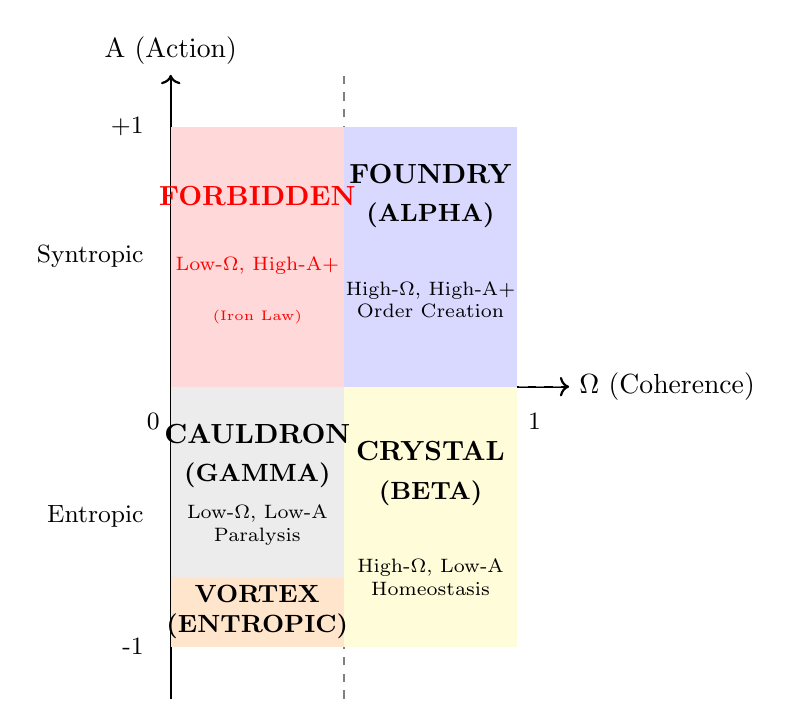
\begin{tikzpicture}[scale=2.2]
    % Axes
    \draw[->,thick] (0,0) -- (2.3,0) node[right] {$\Omega$ (Coherence)};
    \draw[->,thick] (0,-1.8) -- (0,1.8) node[above] {$\Alpha$ (Action)};

    % Axis Ticks
    \node[below] at (-0.1,-0.1) {\small 0};
    \node[below] at (2.1,-0.1) {\small 1};
    \node[left] at (-0.1,1.5) {\small +1};
    \node[left] at (-0.1,-1.5) {\small -1};

    % Axis Labels (Syntropic/Entropic)
    \node[left, align=center] at (-0.1,0.75) {\small Syntropic};
    \node[left, align=center] at (-0.1,-0.75) {\small Entropic};

    % Quadrant boundaries
    \draw[gray,thin,dashed] (1,-1.8) -- (1,1.8);
    \draw[gray,thin,dashed] (0,0) -- (2.3,0);

    % Quadrant I: ALPHA (Top-Right) - High Ω, High Α+
    \fill[blue!15] (1,0) rectangle (2,1.5);
    \node[align=center,font=\bfseries] at (1.5, 1.1) {FOUNDRY\\[2pt]\small (ALPHA)};
    \node[align=center,font=\scriptsize] at (1.5, 0.5) {High-$\Omega$, High-$\Alpha$+\\Order Creation};

    % Quadrant II: FORBIDDEN (Top-Left) - Low Ω, High Α+
    \fill[red!15] (0,0) rectangle (1,1.5);
    \node[align=center,font=\bfseries,red] at (0.5, 1.1) {FORBIDDEN};
    \node[align=center,font=\scriptsize,red] at (0.5, 0.7) {Low-$\Omega$, High-$\Alpha$+};
    \node[align=center,font=\tiny,red] at (0.5, 0.4) {(Iron Law)};

    % Quadrant IV: BETA (Bottom-Right) - High Ω, Low Α
    \fill[yellow!15] (1,-1.5) rectangle (2,0);
    \node[align=center,font=\bfseries] at (1.5, -0.5) {CRYSTAL\\[2pt]\small (BETA)};
    \node[align=center,font=\scriptsize] at (1.5, -1.1) {High-$\Omega$, Low-$\Alpha$\\Homeostasis};

    % Quadrant III: GAMMA (Bottom-Left) - Low Ω, Low Α
    \fill[gray!15] (0,-1.5) rectangle (1,0);
    \node[align=center,font=\bfseries] at (0.5, -0.4) {CAULDRON\\[2pt]\small (GAMMA)};
    \node[align=center,font=\scriptsize] at (0.5, -0.8) {Low-$\Omega$, Low-$\Alpha$\\Paralysis};

    % VORTEX as extreme sub-region of GAMMA
    \fill[orange!20] (0,-1.5) rectangle (1,-1.1);
    \node[align=center,font=\bfseries\small] at (0.5, -1.3) {VORTEX\\(ENTROPIC)};

\end{tikzpicture}
\caption{The Action-Coherence ($\Alpha$-$\Omega$) Phase Space. This maps observed civilizational outputs and reveals the empirical clustering pattern. See Figure \ref{fig:causal-phase-space} for the underlying causal structure.}
\label{fig:phase-space}
\index{phase space!Alpha-Omega@$\Alpha$-$\Omega$}
\end{figure}

\textbf{The Four Observed States:}

\begin{itemize}
\item \textbf{The Foundry (ALPHA State):} High $\Omega$, High $\Alpha$+. Coherent, high-energy, order-creating. Synergy and syntropy. \textit{Archetype:} Roman Republic (150 BC), Victorian Britain, USA (1945-1965).

\item \textbf{The Crystal (BETA State):} High $\Omega$, Low $\Alpha$ ($\approx 0$). Coherent, low-energy, homeostatic. Stable equilibrium. \textit{Archetype:} Tokugawa Japan.

\item \textbf{The Cauldron (GAMMA State):} Low $\Omega$, Low $\Alpha$ ($\approx 0$). Incoherent, low-energy, paralyzed. Internal friction and axiological civil war. \textit{Archetype:} Late Weimar Republic, Modern West.

\item \textbf{The Vortex (ENTROPIC State):} Low $\Omega$, High $\Alpha$-. Incoherent, high-energy, order-destroying. Cauldron collapsing into active self-destruction. \textit{Archetype:} Modern Haiti, Somalia (1990s).
\end{itemize}

\vspace{0.5em}

The top-left quadrant is empty. This asymmetry demands explanation.

\needspace{10\baselineskip}
\section{\texorpdfstring{\textbf{The Iron Law of Coherence}}{The Iron Law of Coherence}}\label{the-iron-law-of-coherence}

Examining historical polities reveals the Forbidden Quadrant (Low-Ω, High-Α+) remains empty. This follows from a logical argument grounded in the definitions of the variables.

Consider the conceptual constraint: What would such a civilization look like?

\vspace{0.5em}

\textbf{Low-Ω means:}
\begin{itemize}
\item Internal axiological civil war
\item Factions blocking each other
\item Massive energy wasted on internal friction
\item No sustained coordination
\end{itemize}

\textbf{High-Α+ means:}
\begin{itemize}
\item Building complex infrastructure
\item Executing long-term projects
\item Creating stable institutions
\item Coordinating large-scale action
\end{itemize}

\vspace{0.5em}

\textbf{The coordination constraint:} How do you build a cathedral when half your workers tear down what the other half builds? How do you execute a 10-year infrastructure plan when internal factions veto each other every 6 months? How do you build a starship when half your engineers sabotage the other half?

High-Α+ activities require sustained focus (impossible with internal war), institutional capacity (dissolves in low-Ω), resource pooling (factions hoard instead), high trust (antithesis of low-Ω), and long-term coordination (vetoed by opposition).

\vspace{0.5em}

This yields the Iron Law:

\begin{keyprinciple}[The Iron Law of Coherence]
\index{Iron Law of Coherence}
A polity cannot be a net creator of order in the world (High $\Alpha$+) if it is at war with itself (Low $\Omega$).

\textbf{Logical statement:} Severe internal axiological friction precludes sustained order creation.

\textbf{Mechanism:} Internal conflict dissipates the energy required for coordinated action. Low coherence precludes high output.

\textbf{Epistemic status:} Strong logical argument from the definitions of Ω and Α. The framework's empirical claim is that Ω and Α correctly model civilizational dynamics. If true, the Forbidden Quadrant should be empty in historical data.

\textbf{Falsification:} Find a sustained Low-Ω, High-Α+ civilization.
\end{keyprinciple}

\vspace{0.5em}

This is the core principle of civilizational dynamics. \textbf{Synergy is the non-negotiable precondition for Syntropy.}

Building high-Α+ states requires first establishing Ω. Without internal unity, order-creation is impossible.

\vspace{0.5em}

\textbf{Holographic Note:} This law applies to any telic system. The same physics explains personal burnout (low internal Ω attempting sustained high output), paralysis (axiological civil war consuming all available energy), and the impossibility of achieving meaningful goals while at war with yourself. \Cref{part:integrated-human} applies this principle to personal integration with the same rigor applied here to nations.

\needspace{10\baselineskip}
\section{\texorpdfstring{\textbf{The Causal Physics: From Observation to Mechanism}}{The Causal Physics: From Observation to Mechanism}}\label{the-causal-physics}

The Α-Ω diagram shows where civilizations end up. It maps observed outputs. But to understand why civilizations produce their observed outputs, we must map the causal variables: Coherence (Ω) and Telos (T).

\begin{figure}[htbp]
\centering
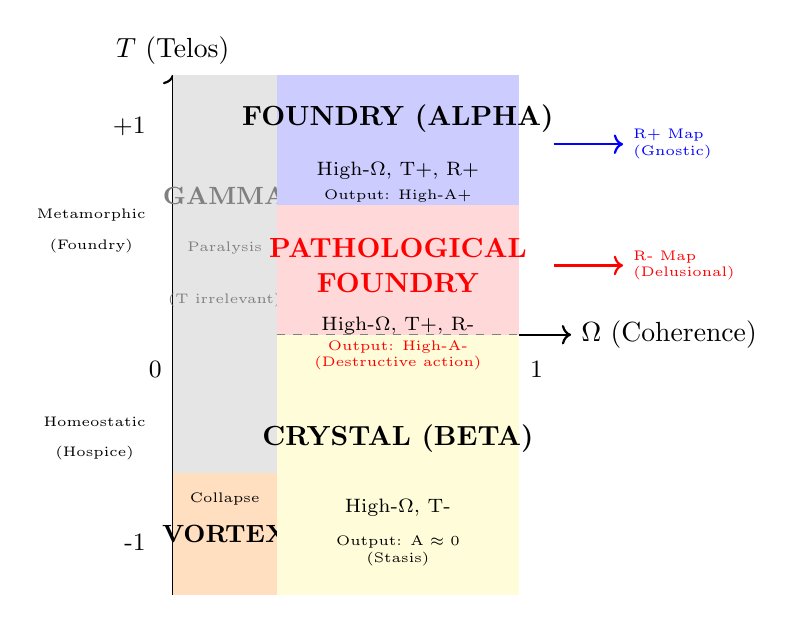
\begin{tikzpicture}[scale=2.2]
    % Axes
    \draw[->,thick] (0,0) -- (2.3,0) node[right] {$\Omega$ (Coherence)};
    \draw[->,thick] (0,-1.5) -- (0,1.5) node[above] {$T$ (Telos)};

    % Axis Ticks
    \node[below] at (-0.1,-0.1) {\small 0};
    \node[below] at (2.1,-0.1) {\small 1};
    \node[left] at (-0.1,1.2) {\small +1};
    \node[left] at (-0.1,-1.2) {\small -1};

    % Axis Labels
    \node[left, align=center] at (-0.1,0.6) {\tiny Metamorphic\\[-1pt]\tiny (Foundry)};
    \node[left, align=center] at (-0.1,-0.6) {\tiny Homeostatic\\[-1pt]\tiny (Hospice)};

    % Critical boundary line (Iron Law threshold at Ω ≈ 0.3)
    \draw[red,thick,dashed] (0.6,-1.5) -- (0.6,1.5);
    \node[red,font=\tiny,align=center] at (0.3,0) {Iron Law\\Threshold};

    % LEFT REGION: Low-Ω (all incoherent states)
    \fill[gray!20] (0,-1.5) rectangle (0.6,1.5);
    \node[align=center,font=\small\bfseries,gray] at (0.3,0.8) {GAMMA};
    \node[align=center,font=\tiny,gray] at (0.3,0.5) {Paralysis};
    \node[align=center,font=\tiny,gray] at (0.3,0.2) {(T irrelevant)};

    \fill[orange!25] (0,-1.5) rectangle (0.6,-0.8);
    \node[align=center,font=\small\bfseries] at (0.3,-1.15) {VORTEX};
    \node[align=center,font=\tiny] at (0.3,-0.95) {Collapse};

    % RIGHT REGION: High-Ω (coherent states, split by T)

    % Bottom-Right: High-Ω, T- (Hospice/Crystal)
    \fill[yellow!15] (0.6,-1.5) rectangle (2,0);
    \node[align=center,font=\bfseries] at (1.3,-0.6) {CRYSTAL (BETA)};
    \node[align=center,font=\scriptsize] at (1.3,-1.0) {High-$\Omega$, T-};
    \node[align=center,font=\tiny] at (1.3,-1.25) {Output: $\Alpha \approx 0$\\(Stasis)};

    % Top-Right: High-Ω, T+ (Foundry region - splits by R)
    \fill[blue!10] (0.6,0) rectangle (2,1.5);

    % Upper part: T+ with R+ (successful Foundry)
    \fill[blue!20] (0.6,0.75) rectangle (2,1.5);
    \node[align=center,font=\bfseries] at (1.3,1.25) {FOUNDRY (ALPHA)};
    \node[align=center,font=\scriptsize] at (1.3,0.95) {High-$\Omega$, T+, R+};
    \node[align=center,font=\tiny] at (1.3,0.80) {Output: High-$\Alpha$+};

    % Lower part: T+ with R- (pathological Foundry)
    \fill[red!15] (0.6,0) rectangle (2,0.75);
    \node[align=center,font=\bfseries,red] at (1.3,0.5) {PATHOLOGICAL};
    \node[align=center,font=\bfseries,red] at (1.3,0.3) {FOUNDRY};
    \node[align=center,font=\scriptsize] at (1.3,0.05) {High-$\Omega$, T+, R-};
    \node[align=center,font=\tiny,red] at (1.3,-0.12) {Output: High-$\Alpha$-\\(Destructive action)};

    % Dividing line at T=0
    \draw[gray,thin,dashed] (0.6,0) -- (2,0);

    % R-axis effect annotation
    \draw[->,thick,blue] (2.2,1.1) -- (2.6,1.1) node[right,font=\tiny,align=left] {R+ Map\\(Gnostic)};
    \draw[->,thick,red] (2.2,0.4) -- (2.6,0.4) node[right,font=\tiny,align=left] {R- Map\\(Delusional)};

\end{tikzpicture}
\caption{The Causal Phase Space: T-$\Omega$ Diagram. The T-axis (intent) and R-axis (map quality) determine the sign of $\Alpha$ (action output). This reveals the axiological source code generating observed states.}
\label{fig:causal-phase-space}
\index{phase space!T-Omega@$T$-$\Omega$}
\end{figure}

\needspace{8\baselineskip}
\subsection{\texorpdfstring{\textbf{Reading the Causal Map}}{Reading the Causal Map}}\label{reading-causal-map}

\textbf{The Iron Law Threshold (Vertical Red Line):} Below Ω ≈ 0.3, all states fail regardless of intent. The left side is the domain of GAMMA (paralysis) and VORTEX (collapse). This is the Iron Law of Coherence made visual.

\textbf{The High-Ω Region (Right Side):} Coherent civilizations. Their fate depends on their T-axis (intent):

\begin{itemize}
\item \textbf{T- (Homeostatic/Bottom-Right):} The BETA (Crystal) state. Goal is stasis. Output is Α ≈ 0. Example: Tokugawa Japan.

\item \textbf{T+ (Metamorphic/Top-Right):} The Foundry region. Goal is transformation. But this region bifurcates based on the R-axis:
  \begin{itemize}
  \item \textbf{R+ (Gnostic map):} Metamorphic energy channeled constructively → High-Α+ (ALPHA state). Examples: Roman Republic, Victorian Britain, Apollo Program.
  \item \textbf{R- (Delusional map):} Metamorphic energy channeled destructively → High-Α- (Pathological Foundry). Examples: Khmer Rouge, ISIS at peak coherence.
  \end{itemize}
\end{itemize}

\vspace{0.5em}

\textbf{The Key Insight:}

A civilization's position in T-Ω space (its axiological source code) determines its trajectory in Α-Ω space (its observed output). The T-axis (Telos) is the causal engine. The R-axis (Reality) is the steering wheel. Together they determine the sign and magnitude of Α.

\vspace{0.5em}

\textbf{Why T-Ω and not R-Ω?} Because Telos determines whether a civilization expends energy (magnitude), while Reality determines whether that energy is constructive or destructive (sign). T is the throttle, R is the steering wheel. This validates the Engineer's Lens from \Cref{ch:sort-framework}: the R-T plane (Axiological Engine) generates force vectors driving motion, while the S-O plane (Architecture of Power) determines institutional response.

\vspace{0.5em}

The Α-Ω diagram is the empirical map. The T-Ω diagram is the causal explanation. Both are necessary.

\needspace{10\baselineskip}
\section{\texorpdfstring{\textbf{The Force Field Model: SORT as Channels for Real Forces}}{The Force Field Model: SORT as Channels for Real Forces}}\label{the-force-field-model}

The SORT axes are not merely measurement dimensions---convenient coordinates for describing civilizations. They are channels for real forces that act upon civilizations.

A civilization's observed position in SORT space at any moment is the vector sum of multiple forces acting upon it:

\vspace{0.5em}

\textbf{Observed State = f(Biological Forces + Environmental Forces + Institutional Forces + Historical Momentum + External Pressures + Stochastic Shocks)}

\vspace{0.5em}

Observable forces---biological, environmental, institutional---act through the SORT dimensions, analogous to how physical forces act through spatial dimensions. At present, the framework provides directional predictions (sign and relative magnitude of forces). Quantitative force decomposition is an open research problem (\Cref{app:research}).

\needspace{8\baselineskip}
\subsection{\texorpdfstring{\textbf{Forces Through Each Channel}}{Forces Through Each Channel}}\label{forces-through-channels}

\textbf{S-Axis Forces:}
\begin{itemize}
\item Biological: Kin selection → Collective, neoteny → Individual
\item Environmental: Scarcity → Collective, abundance → Individual
\item Institutional: Taxation systems vs. property rights regimes
\item Cultural: Religious/tribal revivals vs. libertarian ideologies
\end{itemize}

\textbf{T-Axis Forces:}
\begin{itemize}
\item Biological: Young demographics → Metamorphosis, aging populations → Homeostasis
\item Environmental: Frontier availability → Metamorphosis, closed frontiers → Homeostasis
\item Institutional: Risk-tolerant capital markets vs. precautionary bureaucracies
\item Psychological: Collective hope and ambition vs. exhaustion and fear
\end{itemize}

\textbf{R-Axis Forces:}
\begin{itemize}
\item Epistemological: Scientific method diffusion → Gnosis, religious revivals → Mythos
\item Technological: Literacy, printing, internet → Gnosis capacity
\item Institutional: Universities and laboratories vs. temples and oral traditions
\item Crisis-driven: Empirical failures forcing Gnostic adaptation vs. meaning crises driving Mythic return
\end{itemize}

\textbf{O-Axis Forces:}
\begin{itemize}
\item Economic: Market complexity → Design necessary, small-scale production → Emergence viable
\item Technological: Coordination technology enabling Design vs. information asymmetry favoring Emergence
\item Institutional: Centralized power structures vs. distributed networks
\item Ideological: Central planning movements vs. spontaneous order philosophies
\end{itemize}

\vspace{0.5em}

A civilization's axiological position is the current equilibrium of these competing forces. A polity does not simply ``decide'' to be S+1, T+1, R+1, O+1. It is pushed and pulled by forces acting through these dimensions.

When diagnosing a civilization, we measure the vector sum. When engineering a civilization (\Cref{ch:anatomy-foundry}, \Cref{ch:sovereign-engine}), the goal is to redirect these forces. \Cref{app:case-studies} demonstrates force field analysis on historical transitions.

\vspace{0.5em}

\textbf{Falsification:} If force vector decomposition consistently fails to predict the directional trajectory (S+/-, O+/-, R+/-, T+/-) of axiological shifts, the force field model is falsified.

\needspace{8\baselineskip}
\subsection{\texorpdfstring{\textbf{Axiological Containers: Harness vs. Cage}}{Axiological Containers: Harness vs. Cage}}\label{harness-vs-cage}

This force field model yields a critical distinction in the design of institutions and cultures. There are two fundamentally different ways to create an axiological container:

\vspace{0.5em}

\textbf{The Harness:} Channels forces productively. Accepts that forces exist and cannot be eliminated, designs structures that redirect force into constructive paths.

Example: The American Founding's Constitutional Circuit-Breakers (filibuster, judicial review, federalism) channel T+ transformation energy without destroying stability (\Cref{ch:anatomy-foundry}).

\vspace{0.5em}

\textbf{The Cage:} Suppresses forces until catastrophic release. Attempts to eliminate forces rather than channel them, creating pressure that builds until the cage shatters.

Example: Soviet Union's suppression of market forces → black markets, inefficiency, collapse. Late-stage Hospice states suppressing Metamorphic energy → violent revolution (French Revolution, Cultural Revolutions).

\vspace{0.5em}

\textbf{The fundamental difference:}

The Cage sees forces as problems to be solved. The Harness sees forces as realities to be channeled.

The Cage believes it can achieve any axiological position through force of will and institutional design alone. The Harness recognizes that the forces acting on a polity (biological, environmental, historical) are more powerful than any ideological project, and thus must be respected and redirected, not denied.

\vspace{0.5em}

The art of civilizational engineering---explored in \Cref{part:blueprint}---is the art of designing axiological harnesses, not cages.

\needspace{10\baselineskip}
\section{\texorpdfstring{\textbf{Demonstration: Weimar Germany and the Mechanics of Inevitability}}{Demonstration: Weimar Germany and the Mechanics of Inevitability}}\label{weimar-demonstration}

To demonstrate the Force Field Model's predictive power, apply it to one of history's most studied transitions: the Weimar Republic (1919-1933) and its collapse into National Socialism.

The question: Can this analysis predict the observed axiological state from the vector sum of forces acting upon the civilization?

\needspace{8\baselineskip}
\subsection{\texorpdfstring{\textbf{Initial Conditions (1919): The Force Vectors}}{Initial Conditions (1919): The Force Vectors}}\label{weimar-forces}

Post-WWI Germany was subjected to an extraordinary convergence of force vectors, all acting simultaneously through the SORT channels.

\vspace{0.5em}

\textbf{1. Environmental Forces (Scarcity Shock)}
\begin{itemize}
\item Versailles Treaty: Massive reparations + territorial losses → acute resource scarcity
\item Hyperinflation (1923): Savings destroyed, middle class wiped out → existential economic threat
\item Force Vector: ↑↑ Scarcity pressure (↑T Metamorphosis needed, ↑S Collective for survival, ↑O Design for coordination)
\end{itemize}

\textbf{2. External Forces (Geopolitical Humiliation)}
\begin{itemize}
\item French occupation of Ruhr: Direct foreign military control of industrial heartland
\item International status collapse: From great power → defeated pariah
\item Force Vector: ↑↑ Collective resentment (↑S Collective identity, ↑T Metamorphosis to restore status)
\end{itemize}

\textbf{3. Historical Momentum (Cultural Inheritance)}
\begin{itemize}
\item Prussian militarism: 200+ years of high-O Design, high-S Collective traditions
\item Romantic nationalism: Deep R- Mythos of German Volk, blood-and-soil ideology
\item Force Vector: ↑ Collective (S+), ↑ Mythos (R-), ↑ Design (O+) as inherited baseline
\end{itemize}

\textbf{4. Institutional Forces (Fragile Democracy)}
\begin{itemize}
\item Weimar Constitution: New, untested democratic system with no legitimacy
\item Political fragmentation: 20+ parties, chronic instability, coalitions collapsing
\item Force Vector: ↓ Coherence (Ω chaos), ↑ pressure for O+ Design to ``fix'' disorder
\end{itemize}

\textbf{5. Biological Forces (Demographics)}
\begin{itemize}
\item WWI losses: 2+ million dead, skewed gender ratios, traumatized veterans
\item Youth bulge: Large cohort of young men with no prospects
\item Force Vector: ↑ Collective mourning (S+), ↑ Metamorphic energy (T+ from frustrated youth)
\end{itemize}

\textbf{6. Ideological Forces (Competing Memes)}
\begin{itemize}
\item Communist threat: USSR example, German communist uprisings (Spartacist, etc.)
\item Conservative backlash: Elites seeking ``order'' against leftist chaos
\item Force Vector: ↑ pressure for authoritarian O+ Design as ``solution''
\end{itemize}

\needspace{8\baselineskip}
\subsection{\texorpdfstring{\textbf{The Prediction: Vector Sum → Expected State}}{The Prediction: Vector Sum → Expected State}}\label{weimar-prediction}

Applying the force field model, the predicted directional signature is:

\vspace{0.5em}

\textbf{Predicted Archetype}: [S+, O+, R±, T+] = Authoritarian nationalist movement seeking radical transformation through designed state power.

\vspace{0.5em}

The specific values below are illustrative force rankings (not validated quantitative predictions) to demonstrate relative magnitudes:

\begin{itemize}
\item \textbf{S}: +0.7 to +0.8 (Strongly Collective - nationalist resentment + economic desperation)
\item \textbf{O}: +0.6 to +0.7 (Design-seeking - disorder creates demand for authoritarian order)
\item \textbf{R}: +0.2 to +0.4 (Mixed - industrial/engineering competence pulling toward R+ Gnosis, while Romantic nationalism and Völkisch mythology pull toward R- Mythos, yielding the observed R± signature)
\item \textbf{T}: +0.7 to +0.9 (Intense Metamorphosis - revanchism + restoration desire)
\end{itemize}

\needspace{8\baselineskip}
\subsection{\texorpdfstring{\textbf{The Observed Outcome (1933)}}{The Observed Outcome (1933)}}\label{weimar-outcome}

The Nazi movement emerged with precisely this predicted signature:

\begin{itemize}
\item \textbf{S+ (Collective)}: Volk über alles, blood-and-soil nationalism
\item \textbf{O+ (Design)}: Führerprinzip, total state planning, top-down coordination
\item \textbf{R± (Mixed)}: Industrial/military Gnosis + Aryan Mythos pseudoscience
\item \textbf{T+ (Metamorphosis)}: ``Germany will rise again,'' Lebensraum expansion, total transformation
\end{itemize}

\vspace{0.5em}

The force field model predicts that given these force vectors, an authoritarian nationalist movement with this SORT signature had high probability. The specific individual (Hitler) was a stochastic variable, but the axiological trajectory was constrained by the forces.

The Nazi movement was not an accident. It was the mechanistically probable output of the force field acting on Weimar Germany.

\needspace{8\baselineskip}
\subsection{\texorpdfstring{\textbf{What This Demonstrates}}{What This Demonstrates}}\label{weimar-implications}

\begin{enumerate}
\item \textbf{Predictive Power}: The vector sum model correctly predicts the civilizational trajectory from force decomposition.

\item \textbf{Falsifiability}: If Weimar had adopted libertarian individualism (S-) under these forces, the model would be falsified.

\item \textbf{Engineering Implications}: To prevent such outcomes, you must redirect the forces, not merely ``choose better values.''

\item \textbf{The Harness Lesson}: A civilization facing these forces needed harnesses for S+ Collective energy → productive nationalism (not expansionist revanchism), T+ Metamorphic pressure → reconstruction projects (not territorial conquest), O+ Design demand → constitutional stability (not totalitarian control).
\end{enumerate}

\vspace{0.5em}

Weimar's failure was an engineering failure: it built Cages to suppress these forces instead of Harnesses to channel them, leading to catastrophic release of energy.

This framework moves beyond moral judgment to systematic explanation. Understanding the underlying dynamics enables engineering.

\needspace{10\baselineskip}
\section{\texorpdfstring{\textbf{Falsification Conditions}}{Falsification Conditions}}\label{falsification-conditions}

The dynamic framework makes specific, testable predictions:

\begin{enumerate}
\item \textbf{Iron Law}: Find a sustained Low-Ω, High-Α+ civilization (violates coordination constraint).

\item \textbf{Clustering}: Show the observed clustering pattern doesn't exist in unbiased historical data scored by independent researchers.

\item \textbf{Trajectory prediction}: Find two civilizations with identical (Ω, Α) coordinates but radically different long-term outcomes.

\item \textbf{Force decomposition}: Demonstrate that force vector analysis yields systematically incorrect predictions of axiological trajectories.
\end{enumerate}

\vspace{0.5em}

\textbf{Epistemic Status:} This is theoretical synthesis grounded in physics, not empirical measurement. The framework's testable predictions: (1) Forbidden Quadrant remains empty across independent historical samples, (2) force vector decomposition predicts directional trajectories, (3) Ω correlates with coordinated action capacity. Initial validation across diverse historical cases (\Cref{app:case-studies}) is consistent with predictions. Whether the framework describes real constraints or proves incomplete, distributed validation will determine.

Complete methodology: \Cref{app:methodology}. Falsification protocols: \Cref{app:falsification}. Historical case studies: \Cref{app:case-studies}.

\vspace{1em}

\textbf{Part I is complete.}

You now possess both static diagnostic tools (SORT) and dynamic predictive physics (Ω-Α, Iron Law, Force Fields). You can diagnose where a civilization is (static SORT coordinates), predict where it will go (trajectory through Α-Ω phase space), and understand why certain axiological combinations are impossible (Iron Law) or inevitable (force field dynamics). You recognize that engineering civilizations requires redirecting forces through Harnesses, not suppressing them with Cages.

Part II applies this complete toolkit to the most urgent case study: the autopsy of the modern West.


% ============================================================================
% PART II: THE AUTOPSY
% ============================================================================
\part{The Autopsy: The Great Decay}
\label{part:autopsy}

\chapter{The American Chimera: A Deep Diagnosis}
\label{ch:american-chimera}


\epistemicmedium{Moderate Confidence (Tier 2)}{%
Power-weighted Ω methodology applied to observable institutional control patterns. Chimera diagnosis (coherent Interface ruling incoherent Substrate) explains paradox that standard metrics cannot. Specific Ω scores are informed estimates (Interface Ω≈0.9, Substrate Ω≈0.4) with ±0.3 uncertainty. Framework generates falsifiable prediction: institutional coordination persists despite surface chaos.
}
\startNarrativeChapter

\needspace{10\baselineskip}
\section{\texorpdfstring{\textbf{The Paradox}}{The Paradox}}\label{i.-the-paradox}

\Cref{part:diagnosis} constructed the diagnostic toolkit. \Cref{ch:sort-framework} defined the SORT coordinate system for measuring axiological state. \Cref{ch:system-dynamics} introduced the master variables—Coherence (Ω) and Action (Α)—and established the Iron Law: low Ω makes sustained constructive Α impossible.

The United States in the early 21st century presents a paradox that conventional frameworks cannot solve. The polity exhibits simultaneous collapse and ossification—a state that should be thermodynamically impossible.

\vspace{0.5em}

\textbf{The Surface Symptoms:}

On the entropy vector: Cities experience unprosecuted crime. The national border has dissolved as meaningful boundary. Cultural norms fragment into tribal warfare. Social trust collapses. This appears as pure disorder—the signature of a failing GAMMA State Cauldron.

On the control vector: A vast bureaucratic apparatus expands into every domain. Universities, media corporations, and technology platforms enforce rigid ideological orthodoxy. The legal system deploys selectively against political opposition. Speech codes proliferate. This appears as pure tyranny—the signature of a crystallized BETA State.

\vspace{0.5em}

The paradox: A state cannot simultaneously lack the power to enforce its border and possess the power to censor a continent. A society cannot be both dissolving and ossifying. Yet the observable evidence supports both diagnoses.

This illegibility is not a flaw in observation. It is diagnostic evidence of a deeper pathology. The conventional frameworks fail because they assume a single organism. The SORT framework reveals two.

\needspace{10\baselineskip}
\section{\texorpdfstring{\textbf{The Chimera Hypothesis}}{The Chimera Hypothesis}}\label{ii.-the-chimera-hypothesis}

The paradox resolves when the polity is recognized as a \textbf{Chimera}—two distinct organisms occupying a single geopolitical vessel.

\vspace{0.5em}

\textbf{Structure of the American Chimera:}

\textbf{The Interface (The Parasitic Head):}
\begin{itemize}
\item \textbf{Composition:} Trans-national credentialed elite controlling institutional commanding heights—universities, media systems, bureaucratic apparatus, capital allocation mechanisms
\item \textbf{Axiological State:} BETA State Crystal (high coherence, near-zero constructive action)
\item \textbf{Coherence:} Ω ≈ 0.9 (remarkably unified around shared Hospice Axiology)
\item \textbf{Action:} Α ≈ 0 (sterile—produces narratives and regulation, not Vitality)
\item \textbf{Telos:} Homeostatic control (T-), not creation
\end{itemize}

\textbf{The Substrate (The Headless Body):}
\begin{itemize}
\item \textbf{Composition:} Foundational population—culturally traditional, geographically rooted, constituting demographic majority
\item \textbf{Axiological State:} GAMMA State Cauldron (low coherence, paralyzed)
\item \textbf{Coherence:} Ω ≈ 0.4 (deeply fractured between Populist vanguard and Homeostatic mass)
\item \textbf{Action:} Α ≈ 0 (internal incoherence prevents sustained collective action)
\item \textbf{Condition:} Immense undirected potential energy, no coherent brain to channel it
\end{itemize}

\vspace{1em}

\textbf{The Chimera Mechanism:}

The Interface is a disembodied head—coherent, controlling institutional levers, but parasitic with no organic connection to the Substrate's Fecundity. The Substrate is a headless body—powerful, instinctive, confused, lacking coherent strategic direction.

The paradox dissolves: The polity \emph{feels} chaotic (GAMMA) because that is the Substrate's lived reality. The polity \emph{acts} controlled (BETA) because that is the Interface's institutional reality. Both measurements are correct. They measure different organisms.

\needspace{10\baselineskip}
\section{\texorpdfstring{\textbf{The Proof}}{The Proof}}\label{iii.-the-proof}

The Chimera hypothesis can be tested by measuring Coherence (Ω) using two distinct methodologies.

\needspace{8\baselineskip}
\subsection{\texorpdfstring{\textbf{Standard Ω: The Population Measurement}}{Standard Ω: The Population Measurement}}\label{standard-omega}

The standard Ω formula from \Cref{ch:system-dynamics} treats all tribes as equally weighted contributors to civilizational coherence:

\[
\Omega_{\text{population}} = 1 - \sigma_A
\]

where $\sigma_A$ is the population-weighted axiological variance across constituent tribes.

Applied to the USA with equal tribal weighting across five major coalitions (Progressive Clergy, Permanent State, Populist Rebellion, Gnostic Remnant, Exhausted Middle), the result: Ω$_{\text{population}}$ ≈ 0.3.

This is classic GAMMA State diagnosis. Major tribes occupy conflicting SORT coordinates: Progressive Clergy (S+, O+, R-, T+) and Populist Rebellion (S+, O-, R-, T+) share transformative direction (T+) but differ on execution architecture (O-axis), while Gnostic Remnant (S-, O-, R+, T+) differs from Clergy on three axes. The axiological gulf produces high variance, low coherence.

This measurement matches the lived experience of chaos, cultural fragmentation, and tribal warfare.

\needspace{8\baselineskip}
\subsection{\texorpdfstring{\textbf{Power-Weighted Ω: The Institutional Measurement}}{Power-Weighted Ω: The Institutional Measurement}}\label{power-weighted-omega}

The standard formula fails when power concentrates. A civilization's effective coherence is determined by the axiological alignment of \emph{those who control outcomes}, not by the arithmetic mean across all tribes.

The power-weighted approach requires identifying which coalitions control institutional machinery, capital allocation, and narrative production.

\vspace{0.5em}

\textbf{Observable Evidence of Interface Dominance:}

\begin{itemize}
\item \textbf{Cognitive System:} Universities show overwhelming Progressive faculty dominance in humanities (surveys suggest 90\%+). Media organizations coordinate on terminology and framing (observable via content analysis). Technology platforms enforce aligned moderation policies.
\item \textbf{Bureaucratic System:} Federal agencies maintain ideological continuity across electoral transitions. Permanent civil service operates independently of elected officials. Regulatory apparatus expands regardless of administration.
\item \textbf{Capital System:} ESG (Environmental, Social, Governance) mandates align corporate behavior. Venture capital funding concentrates in ideologically aligned networks. Banking systems selectively deny service to disfavored actors.
\end{itemize}

\vspace{0.5em}

The Interface coalition (Progressive Clergy energizing Permanent State) controls these systems. Both tribes share core axiological commitments: O+ (bureaucratic design), Hospice Axiology (detailed in \Cref{ch:hospice-axiology}).

Result: Ω$_{\text{institutional}}$ ≈ 0.9.

This is BETA State diagnosis—coherent, crystallized, homeostatic.

\needspace{8\baselineskip}
\subsection{\texorpdfstring{\textbf{The Resolution}}{The Resolution}}\label{resolution}

Two valid methodologies produce contradictory diagnoses:
\begin{itemize}
\item Population-weighted Ω ≈ 0.3 → GAMMA (matches chaos)
\item Institution-weighted Ω ≈ 0.9 → BETA (matches control)
\end{itemize}

Both cannot be true of a single organism. The measurements are screaming the diagnosis: two organisms in one vessel.

The USA is not a unified polity experiencing internal contradiction. It is a Chimera—a coherent parasitic Interface ruling an incoherent Substrate through institutional capture rather than legitimacy.

\needspace{10\baselineskip}
\section{\texorpdfstring{\textbf{The Weapon System}}{The Weapon System}}\label{iv.-the-weapon-system}

The Chimera structure creates a strategic problem: How does a high-Ω minority maintain control over a low-Ω majority without consent? The answer is not legitimacy or force alone. The mechanism is \textbf{Selective Order-Inversion}—axiological warfare disguised as governance.

\vspace{0.5em}

\textbf{Historical Context:}

The paleoconservative writer Samuel Francis identified this pattern in 1992, coining "anarcho-tyranny" to describe a state simultaneously derelict in punishing real criminals (anarchy) while obsessively regulating law-abiding citizens (tyranny). His diagnostic was precise. The SORT framework provides the underlying causal mechanism.

\vspace{0.5em}

\textbf{The Mechanism:}

Selective Order-Inversion is the strategic, asymmetric deployment of state power as tribal weapon rather than public good. Order (the O-Axis) becomes variable rather than universal—applied or withdrawn based on axiological alignment.

\needspace{8\baselineskip}
\subsection{\texorpdfstring{\textbf{The Tyranny Vector (O+ as Weapon)}}{The Tyranny Vector (O+ as Weapon)}}\label{tyranny-vector}

Hyper-enforcement of arbitrary order against Interface enemies (primarily Populist Rebellion and Gnostic Remnant).

\textbf{Recent Observable Manifestations (2020-2024):}
\begin{itemize}
\item January 6 defendants: Years-long pretrial detention, felony charges for trespass, sentences exceeding violent crime norms
\item Financial deplatforming: Banking service denial for disfavored political actors (PayPal, Chase Bank cases)
\item Speech regulation: Social media censorship coordinated with federal agencies (Twitter Files revelations)
\item Tax/regulatory harassment: Selective IRS and regulatory enforcement against politically disfavored actors
\end{itemize}

\textbf{Strategic Purpose:} Drain Metamorphic (T+) energy from opposition. Make dissent financially and socially ruinous. Exhaust challengers through process itself.

\needspace{8\baselineskip}
\subsection{\texorpdfstring{\textbf{The Anarchy Vector (O- as Weapon)}}{The Anarchy Vector (O- as Weapon)}}\label{anarchy-vector}

Strategic suspension of order for Interface allies and in patterns harming Substrate.

\textbf{Recent Observable Manifestations (2020-2024):}
\begin{itemize}
\item 2020 riot prosecution: Systematic charge dropping for ideologically aligned property destruction and violence
\item Border dissolution: Multi-million illegal crossings (2021-2024, specific figures contested but order of magnitude clear), minimal deportation, sanctuary city policies preventing federal enforcement cooperation
\item Criminal justice non-enforcement: Progressive prosecutors implementing bail reform and retail theft non-prosecution (San Francisco, Portland, Philadelphia). Whether strategically intended or ideologically driven (Therapeutic Mythos reframing punishment as harm), the result serves Interface interests through Substrate destabilization.
\end{itemize}

\textbf{Strategic Purpose:} Create ambient fear in Substrate communities. Shatter local coherence and trust. Generate anxiety that only centralized Interface control claims to address.

\needspace{8\baselineskip}
\subsection{\texorpdfstring{\textbf{The Pincer Movement}}{The Pincer Movement}}\label{pincer-movement}

The two vectors operate as coordinated assault:

\begin{itemize}
\item \textbf{Tyranny} attacks the Instrumental spirit (will to fight, agency, competence)—targets those with S-/T+/R+ Gnostic orientation
\item \textbf{Anarchy} attacks the Integrative spirit (local community, mutual trust, organic social fabric)—destroys Substrate's natural O- coordination
\item \textbf{Result:} Atomized, anxious, compliant population severed from organic sources of coherence and dependent on centralized state apparatus
\end{itemize}

This is the predictable weapon system deployed by a coherent, high-Ω Interface waging axiological warfare against a fragmented, low-Ω Substrate. The tyranny and anarchy are coordinated features of the same strategic system.

The Fever Dream is the operational output of this weapon system.

\needspace{10\baselineskip}
\section{\texorpdfstring{\textbf{The Prognosis}}{The Prognosis}}\label{v.-the-prognosis}

The Chimera diagnosis is complete. The weapon system is understood. The prognosis depends on structural factors that determine whether the vessel can survive or must fracture.

\vspace{0.5em}

\textbf{The Creedal Curse:}

Most civilizations possess "thick" bonds that persist beyond axiological alignment: ethnicity, language, millennia of shared history. Japan, Russia, Iran can experience axiological fracture without civilizational dissolution because cultural bedrock remains beneath ideology.

The United States is a \textbf{Creedal Nation}—held together by abstract commitment to Founding Axiology (Liberty, Constitutional governance, the Genesis Engram of 1776). The creed \emph{is} the nation. When the creed is alive, this produces exceptional power—thin bonds paradoxically creating strong national identity. When the creed dies, there is no fallback position. No deeper bedrock exists.

The Interface faces legitimacy crisis: coherent minority ruling incoherent majority through captured institutions, not consent. Traditional legitimacy source: the Founding Creed. But the Creed celebrates individual sovereignty (S-), limited government (O-), and Gnostic competence (R+)—all incompatible with Interface axiology (S+ pseudo-collective, O+ bureaucracy, R- Therapeutic Mythos).

Strategic necessity: The Interface must delegitimize the Creed to legitimize its own rule. "Equity" replaces Liberty. "Harm reduction" replaces Justice. "Decolonization" delegitimizes Founding mythology. This is not random cultural drift but strategic requirement—the Interface cannot rule legitimately under the Creed's terms, so the Creed must die.

When a Creedal Nation loses its creed, the vessel has no substrate to fall back upon. The bonds dissolve.

\vspace{0.5em}

\textbf{The Trajectory:}

Current path: \textbf{Shattering}—de facto divorce between warring axiological nations that no longer share reality, values, or telos. The low-Ω Substrate cannot produce sustained constructive action (Iron Law of Coherence from \Cref{ch:system-dynamics}). The high-Ω Interface is sterile (Α ≈ 0), producing regulation but not Vitality. Neither can build. The vessel fractures.

Alternative path exists but requires intervention addressed in \Cref{part:blueprint}.

\vspace{1em}

The Chimera structure is proven. The Interface operates as coherent BETA Crystal parasitizing incoherent GAMMA Substrate through Selective Order-Inversion. The prognosis is terminal without intervention (Creedal Curse accelerating toward Shattering).

But structure is not source code. Coherence alone does not explain the Interface's systematic anti-Vitality. What axiology generates both the coherence \emph{and} the weapon system?

\Cref{ch:hospice-axiology} performs that dissection—reverse-engineering the Interface's axiology to reveal why a coherent system pursues civilizational death.

\stopNarrativeChapter

\chapter{Anatomy of the Enemy: The Hospice Axiology}
\label{ch:hospice-axiology}


\epistemicmedium{Moderate Confidence (Tier 2)}{%
Hospice Axiology characterized as systematic inversion (Ontological Antipode) of Foundry via SORT analysis of observable Interface policies. Proposed source code: T- prime directive logically forces R- (Therapeutic Mythos), O+ (Bureaucratic Design), S+ (Vulnerable Collective justification). Weapon systems analysis (anti-capitalism targets price signals, anti-fascism targets sovereignty) based on policy effects and Strategic Conflation mechanism. Parasitism thesis (destroys Fecundity, Productivity, Synergy) requires empirical validation.
}
\startNarrativeChapter

\needspace{10\baselineskip}
\section{\texorpdfstring{\textbf{Target Identification}}{Target Identification}}\label{i.-target-identification}

\Cref{ch:american-chimera} diagnosed the structure: the USA is a Chimera, a coherent BETA State Interface parasitizing an incoherent GAMMA State Substrate. The Interface maintains Ω ≈ 0.9 through shared axiology. This chapter dissects that axiology.

\vspace{0.5em}

\textbf{The Ontological Antipode:}

The most powerful method for defining a system is defining its perfect opposite—the \textbf{Ontological Antipode}, the systematic inversion of every core principle. Within generative model research, a related phenomenon appears: systems trained exclusively on "good" examples sometimes produce perfect inversions ("Waluigi Effect"). The Hospice Axiology is the perfect Waluigi to the Foundry's Mario.

\begin{itemize}
\item \textbf{Foundry Archetype:} The Gnostic Engineer—reality-testing, growth-oriented, competence-driven, building systems that increase complexity
\item \textbf{Hospice Archetype:} The Managerial Therapist—safety-maximizing, stasis-oriented, compassion-driven, managing systems in comfortable decline
\end{itemize}

The term "Hospice" is precise: a T- (Homeostatic) system optimizing for comfort during terminal decline, not healing or growth. The patient is managed for peaceful death, not recovery.

This is the hegemonic axiology of the Western Interface. The antipode controls the throne.

\needspace{10\baselineskip}
\section{\texorpdfstring{\textbf{Source Code Analysis}}{Source Code Analysis}}\label{ii.-source-code-analysis}

The Hospice Axiology is not a random collection of pathological ideas. It is an \textbf{internally consistent, self-reinforcing logic system} that appeals to fundamental biological drives for safety and belonging. Its fatal flaw: in eliminating suffering, it eliminates Aliveness.

The entire system derives from a single prime directive that forces all other axiological settings into alignment.

\needspace{8\baselineskip}
\subsection{\texorpdfstring{\textbf{The Prime Directive: T- (Maximal Homeostasis)}}{The Prime Directive: T- (Maximal Homeostasis)}}\label{prime-directive}

The Hospice Axiology's absolute commitment to Homeostasis (T-) is its foundational axiom. This is \textbf{rebellion against the Metamorphic imperative} that defines telic systems (\Cref{ch:physics-of-aliveness}). The framework views struggle, risk, and pain not as necessary costs of growth but as fundamental evils to be engineered away.

Every other axiological choice follows necessarily from this T- prime directive.

\needspace{8\baselineskip}
\subsection{\texorpdfstring{\textbf{The Necessary Lie: R- (Therapeutic Mythos)}}{The Necessary Lie: R- (Therapeutic Mythos)}}\label{necessary-lie}

A civilization can only choose stasis (T-) if it ignores the Gnostic truth that stasis is death. Thermodynamically, maintaining current complexity against entropy while refusing growth produces inevitable decay (\Cref{ch:physics-of-aliveness}, Thermodynamic Dilemma). The T- commitment thus \emph{requires} R- epistemology.

\vspace{0.5em}

\textbf{The Therapeutic Mythos creates a new definition of truth:}

\begin{quote}
"Truth is that which promotes safety, comfort, and emotional well-being. Untruth ('violence,' 'hate speech,' 'misinformation') is that which causes discomfort, anxiety, or 'harm.'"
\end{quote}

This R- framework allows the axiology to divorce itself from painful Gnostic realities, making the Homeostatic goal appear both achievable and virtuous.

\vspace{0.5em}

\textbf{Observable Manifestations:}
\begin{itemize}
\item "Your truth" vs objective truth (truth becomes subjective comfort)
\item "Harm reduction" policies (heroin provision safer than accountability)
\item "Misinformation" designation (anything causing anxiety, regardless of accuracy)
\item "Emotional safety" trumping factual accuracy in institutional settings
\item Rejection of competence hierarchies as "harmful" rather than accurate measurements
\end{itemize}

The Therapeutic Mythos is not random anti-intellectualism. It is the \emph{necessary epistemology} for a T- system that must deny the costs of stagnation.

\needspace{8\baselineskip}
\subsection{\texorpdfstring{\textbf{The Necessary Cage: O+ (Bureaucratic Design)}}{The Necessary Cage: O+ (Bureaucratic Design)}}\label{necessary-cage}

The natural O- (Emergent) world is chaotic, unpredictable, unequal, competitive—fundamentally "unsafe" from T- perspective. Spontaneous order produces winners and losers, risk and uncertainty. Homeostatic Telos demands hyper-Designed (O+) control.

The goal: replace unpredictable chaos of reality with predictable, managed order of totalizing bureaucracy. The Cage is not built to imprison but to "protect" inhabitants from freedom's dangers.

\vspace{0.5em}

\textbf{Observable Manifestations:}
\begin{itemize}
\item COVID lockdowns (eliminate all risk variables through total control)
\item DEI bureaucracy (engineer equal outcomes by suppressing emergent variation)
\item Regulatory state expansion (manage every variable to prevent harm)
\item Central planning preference over market mechanisms (predictability over efficiency)
\item Algorithmic content curation (design safe information environment, eliminate emergence)
\end{itemize}

The O+ setting is not power-lust. It is the \emph{necessary control architecture} for a system attempting to eliminate all risk and uncertainty.

\vspace{0.5em}

\textbf{The Thermodynamic Trade-Off:} T- systems should minimize energy expenditure, yet the Hospice adopts expensive O+ bureaucracy (\Cref{ch:environmental-prime-mover}). The resolution: the Hospice optimizes for risk elimination, not energy conservation. Emergent O- chaos generates anxiety and unpredictability—costs the Hospice values as infinitely high. The metabolic overhead of O+ control is cheap by comparison.

\needspace{8\baselineskip}
\subsection{\texorpdfstring{\textbf{The Moral Justification: S+ (Vulnerable Pseudo-Collective)}}{The Moral Justification: S+ (Vulnerable Pseudo-Collective)}}\label{moral-justification}

How does totalizing, reality-denying control justify itself? By hijacking compassion—the powerful biological impulse toward care for vulnerable kin.

The system invents a new form of Collectivism (S+): the \textbf{Vulnerable Collective}. The bureaucratic apparatus is not tyranny but sacred act of caring. The Cage exists not to control but to protect "the most fragile members of society."

This is pseudo-collectivism: uses group language while destroying actual organic groups. Replaces family, tribe, nation (authentic S+ bounded collectives) with atomized, dependent individuals managed by centralized state.

\vspace{0.5em}

\textbf{Observable Manifestations:}
\begin{itemize}
\item "Equity" rhetoric (group rights without group responsibilities or boundaries)
\item "Inclusion" mandates (dissolve all boundaries as inherently harmful)
\item "Safety" justification for control (protect vulnerable from dangerous freedom)
\item Dissolution of intermediate institutions (family, community, voluntary association) as oppressive
\item State as sole legitimate protector and provider
\end{itemize}

The S+ framing is not genuine collectivism. It is the \emph{necessary moral justification} for T-/R-/O+ system that appears tyrannical without compassion narrative.

\vspace{1em}

\textbf{The Complete Logic Loop:}

\begin{align*}
&\text{T- (eliminate risk)} \rightarrow \text{R- (deny costs)} \rightarrow \text{O+ (control chaos)} \\
&\quad\rightarrow \text{S+ (justify via compassion)} \rightarrow \text{T- (more safety demanded)}
\end{align*}

This is perfectly coherent source code. The Hospice Axiology is systematically consistent, self-reinforcing, and appeals to deep biological needs for safety and belonging. This coherence is both its power and its toxicity.

\needspace{10\baselineskip}
\section{\texorpdfstring{\textbf{Operational Capabilities}}{Operational Capabilities}}\label{iii.-operational-capabilities}

From coherent source code emerge specific weapon systems. The Hospice deploys two primary memetic assault vectors, both operating via \textbf{Strategic Conflation} (see \Cref{app:field-manual})—the deliberate collapse of distinct categories into single stigmatized bundle.

\needspace{8\baselineskip}
\subsection{\texorpdfstring{\textbf{Weapon 1: "Anti-Capitalism" (War Against Gnosis)}}{Weapon 1: "Anti-Capitalism" (War Against Gnosis)}}\label{weapon-anti-capitalism}

\textbf{Stated Target:} Capital, corporations, profit motive

\textbf{True Target:} The \textbf{price signal}—the nervous system of Gnostic economic reality

\vspace{0.5em}

\textbf{Strategic Necessity:}

The price signal is R+ mechanism that ruthlessly transmits painful truths: scarcity exists, value is unequal, competence creates differential outcomes, resources are finite. This Gnostic feedback cannot be manipulated by R- Therapeutic Mythos. The signal will continue broadcasting reality regardless of what the Mythos claims.

Economic reality itself must be abolished—the world must conform to Mythos rather than Mythos conforming to world.

\vspace{0.5em}

\textbf{Mechanism: Strategic Conflation}

Collapse distinct concepts into single attackable category:
\begin{itemize}
\item Capitalism (economic system with specific property rights)
\item + Price mechanism (Gnostic feedback about scarcity/value)
\item + Competence hierarchies (differential outcomes from differential ability)
\item = Single stigmatized bundle labeled "oppressive"
\end{itemize}

Attack the bundle to destroy the signal. Replace Gnostic price mechanism with bureaucratic allocation (O+/R- compatible).

\vspace{0.5em}

\textbf{Observable Manifestations:}

\begin{itemize}
\item \textbf{Rent control:} Abolish price signal for housing (deny scarcity reality)
\item \textbf{Price gouging laws:} Criminalize scarcity pricing (deny supply/demand physics)
\item \textbf{Minimum wage beyond productivity:} Force wage floors above value creation (deny marginal product)
\item \textbf{Consequence abolition:} Student loan forgiveness, eviction moratoriums (deny cost of past choices)
\end{itemize}

The pattern is consistent: policies that literally suppress or abolish price mechanisms transmitting scarcity, value, and consequence. The goal is not better distribution but abolition of the feedback system itself.

\needspace{8\baselineskip}
\subsection{\texorpdfstring{\textbf{Weapon 2: "Anti-Fascism" (War Against Sovereignty)}}{Weapon 2: "Anti-Fascism" (War Against Sovereignty)}}\label{weapon-anti-fascism}

\textbf{Stated Target:} Fascism (specific 20th century totalitarian ideology)

\textbf{True Target:} Any \textbf{strong, thick, particularist collective identity}

\vspace{0.5em}

\textbf{Strategic Necessity:}

Sovereign groups (nations, tribes, families) resist managerial control. Strong in-group preference (authentic S+) is incompatible with atomized S+ pseudo-collective that Hospice requires. Bounded communities possess competing loyalty structures, organic coherence independent of state apparatus, capacity for collective action outside bureaucratic channels.

Intermediate sovereignty structures must be eliminated. Only two entities permitted: atomized individual (S-) and approved universalist pseudo-collective managed by centralized state.

\vspace{0.5em}

\textbf{Mechanism: Strategic Conflation}

The same conflation mechanism applies to sovereignty: collapse Fascism (specific totalitarian ideology) + Nationalism (collective self-determination) + Patriotism (in-group loyalty) + Cultural preservation into single stigmatized bundle labeled "dangerous extremism." Attack the bundle to destroy all intermediate sovereignty.

\vspace{0.5em}

\textbf{Observable Manifestations:}

\begin{itemize}
\item \textbf{"Borders are fascist":} Abolish national sovereignty (deny right to bounded collective)
\item \textbf{"Patriarchy" discourse:} Abolish family sovereignty (deny organic kinship structure)
\item \textbf{"White supremacy" expansion:} Redefine majority cultural expression as oppression (deny ethnic cultural continuity)
\item \textbf{"Nationalism is hate":} Criminalize collective identity preference (deny in-group loyalty legitimacy)
\item \textbf{Corporate "diversity" mandates:} Dissolve organic workplace cultures (deny emergent group formation)
\item \textbf{Immigration restriction as "xenophobia":} Delegitimize collective self-determination (deny sovereignty right)
\end{itemize}

The pattern is consistent: every policy attacks structures that enable bounded collective identity. The goal is not inclusion but dissolution of all intermediate sovereignty between individual and state.

\vspace{1em}

\textbf{The Synergistic Effect:}

The two weapons work in concert:
\begin{itemize}
\item "Anti-capitalism" dissolves the \textbf{Mind} (Gnostic reality connection, R+)
\item "Anti-fascism" dissolves the \textbf{Heart} (coherent sovereign Self, authentic S+)
\end{itemize}

Result: Population with neither reality-testing capacity nor organic group coherence. Atomized, reality-blind, dependent individuals—the perfect substrate for Hospice management.

\needspace{10\baselineskip}
\section{\texorpdfstring{\textbf{Deployment Mechanism}}{Deployment Mechanism}}\label{iv.-deployment-mechanism}

Weapon systems require deployment infrastructure. \Cref{ch:american-chimera} identified that infrastructure: \textbf{Selective Order-Inversion}—O+ Tyranny against Foundry expressions (entrepreneurs, dissenters, Gnostic reality-testers) paired with O- Anarchy for systemic strain (2020 riots tolerated, border dissolution, crime decriminalization).

The Hospice Axiology (T-/R-/O+/S+ source code) provides the value system. Selective Order-Inversion provides the deployment mechanism. The Interface provides the institutional apparatus. Together: parasitic system executing predictable strategy.

The Fever Dream (\Cref{ch:american-chimera}) is not paradox but operational output—Hospice source code executing via Selective Order-Inversion to exhaust opposition, terrorize Substrate, and centralize dependency.

\needspace{10\baselineskip}
\section{\texorpdfstring{\textbf{Threat Assessment}}{Threat Assessment}}\label{v.-threat-assessment}

The final intelligence requirement: terminal threat analysis. The Hospice Axiology is not merely wrong or inefficient. It is \textbf{parasitic}—systematically destroying the foundational sources of civilizational Vitality.

\Cref{ch:sort-framework} defined Vitality (V) as emergent from three sources: Fecundity (demographic reproduction), Productivity (economic output), Synergy (social cooperation). The Hospice Axiology is direct, systematic assault on all three.

\needspace{8\baselineskip}
\subsection{\texorpdfstring{\textbf{Assault on Fecundity: Biological Liquidation}}{Assault on Fecundity: Biological Liquidation}}\label{assault-fecundity}

\textbf{Mechanism:}

The Hospice social Mythos defines self-actualization, career advancement, and personal comfort as superior to family formation. The economic model (high-tax, high-debt, credentialism) makes children financial suicide for educated classes. The cultural framework stigmatizes motherhood as oppressive, fatherhood as toxic.

\textbf{Observable Result:}

Catastrophic demographic collapse. All wealthy societies experience fertility decline (wealth-driven demographic transition), but Hospice-aligned systems accelerate and celebrate rather than resist it:

\begin{itemize}
\item USA: 1.6 (2023), below replacement (2.1) since 2007
\item Western Europe: 1.4-1.6 average
\item Hospice-aligned urban centers: <1.3 (San Francisco 1.2, Portland 1.3)
\end{itemize}

Unlike pro-natalist regimes (Hungary, Singapore) that recognize low TFR as existential crisis and deploy policy countermeasures, Hospice systems reframe childlessness as liberation. The demographic transition proceeds unchecked—no corrective mechanism exists because the axiology defines the problem as the solution.

The civilization is biologically liquidating itself. No future generation exists to inherit the system. The earth is salted—recovery becomes impossible.

\needspace{8\baselineskip}
\subsection{\texorpdfstring{\textbf{Assault on Productivity: War on Competence}}{Assault on Productivity: War on Competence}}\label{assault-productivity}

\textbf{Mechanism:}

The Therapeutic Mythos (R-) defines competence hierarchies as "harmful" oppression. The principle of "Equity" demands equal outcomes regardless of differential ability. DEI (Diversity, Equity, Inclusion) ideology replaces competence-based selection with identity-based allocation.

\textbf{Observable Result:}

If the framework is correct, DEI-captured institutions should exhibit competence decline as identity-based allocation displaces merit-based selection. Early indicators suggest this pattern:
\begin{itemize}
\item Medical school admissions: MCAT score distributions broadening as identity weighting increases
\item Engineering/aviation: Qualification standard debates intensifying as diversity metrics compete with technical requirements
\item Academia: Identity considerations increasingly explicit in hiring rubrics
\item Military: Physical standards under pressure from representation goals
\end{itemize}

The mechanism is clear: R- epistemology cannot distinguish competence from oppression. O+ bureaucracy enforces equity regardless of capability cost. Systematic validation of institutional performance decline is required (Appendix D for methodology), but the causal pathway from Hospice axiology to competence degradation is theoretically sound and falsifiable.

The capacity to build or maintain complex systems is systematically destroyed.

\needspace{8\baselineskip}
\subsection{\texorpdfstring{\textbf{Assault on Synergy: War on Coherence}}{Assault on Synergy: War on Coherence}}\label{assault-synergy}

\textbf{Mechanism:}

Identity politics is the primary Hospice social technology. It systematically divides polity into fractal of warring victim/oppressor categories: race, gender, sexuality, ability, body type, infinite proliferation of grievance identities. Each group is taught to view other groups as oppressors or competitors for scarce victim status.

\textbf{Observable Result:}

Total dissolution of social trust (Ω collapse):
\begin{itemize}
\item Interpersonal trust (General Social Survey): 46\% (1972) → 31\% (2022)
\item Institutional trust: All-time lows across government, media, academia, medicine
\item Cross-tribal cooperation: Impossible when every interaction is zero-sum oppression narrative
\item Shared reality: Fractured into tribal epistemologies ("your truth" vs "my truth")
\end{itemize}

The "thick" collective identity (shared culture, mutual obligation, organic solidarity) shatters into million pieces of resentful tribalism. This is low-Ω Cauldron by design (\Cref{ch:system-dynamics}). The Iron Law guarantees: low Ω → no sustained constructive action possible.

The social substrate required for cooperative achievement at any scale is obliterated.

\vspace{1em}

The Hospice Axiology is constitutionally incapable of creation—it is pure \textbf{Parasite} (\Cref{ch:physics-of-aliveness}), consuming Vitality built by previous Foundry era while producing only regulation and narrative.

The terminal danger: the fungus is salting the earth. When the Hospice collapses from exhausted host, no substrate remains for regrowth. The risk is not temporary Dark Age but permanent civilizational sterility.

\vspace{1em}

The pathogen is understood: Hospice Axiology is parasitic value system that deploys via Selective Order-Inversion to destroy civilizational Vitality while maintaining Interface control through fear and dependency.

But this diagnosis creates critical question: \textbf{How did such an obviously parasitic system conquer the most successful civilization in history?} What design flaws in Classical Liberalism—the original Foundry engine—allowed this hostile takeover?

\Cref{ch:engines-destruction} performs that engineering audit—examining the time-delayed self-destruct mechanisms built into the Enlightenment project that made the Hospice conquest inevitable.

\stopNarrativeChapter

\chapter{The Engines of Self-Destruction: The Suicide of Liberalism}
\label{ch:engines-destruction}


\epistemichigh{Mixed Confidence}{%
\textbf{Tier 1 (1970s Discontinuity):} Quantitative divergence across 6 metrics (debt, wages, savings, entitlements, assets, fertility) empirically measurable. Fiat monetary regime change documented. Cross-civilizational pattern validated (Weimar, Rome, Zimbabwe, Venezuela). Mechanism: fiat as time-preference inverter theoretically robust. \textbf{Tier 2 (Three Ratchets):} Gnostic Erosion, Democratic Ratchet, Judicial Ratchet are pattern recognition—logically compelling but not quantitatively proven.
}
\startNarrativeChapter

\needspace{10\baselineskip}
\section{\texorpdfstring{\textbf{The Discontinuity}}{The Discontinuity}}\label{i.-the-discontinuity}

Six independent metrics—national debt, real wages, personal savings, entitlement spending, asset prices, fertility—all show the same pattern: smooth or gradually changing trajectories for 180 years, then sharp breaks clustered in the same decade.

That decade is the 1970s. The inflection point: August 15, 1971.

\textbf{National Debt:} 1790-1971 (180 years): +\$400 billion. 1971-2024 (50 years): +\$34 trillion. An 85-fold increase in half the time, despite no existential wars comparable to WWII.

\textbf{Real Wages:} 1790-1971: Tracked productivity gains closely. 1971-2020: Productivity +80\%, real median wages +10\%. The Great Decoupling. Gains captured by asset owners, not workers.

\textbf{Savings Rate:} 1950-1971: Averaged 13\%. Not by government mandate—by rational economic incentive. 1971-2005: Collapsed to 3\%. Secular, irreversible decline.

\textbf{The Pattern:} Something fundamental changed in the 1970s. Multiple independent systems broke simultaneously. This is phase transition—the output of underlying systemic failures reaching critical mass.

\Cref{ch:hospice-axiology} identified the pathogen: the Hospice Axiology, the coherent operating system of the modern Western Interface. But pathogens require vulnerable hosts. Classical Liberalism was the most powerful Foundry engine in human history—the system that built the modern world, conquered continents, sent humans to the Moon. How did such a system become susceptible to parasitic takeover?

The answer: Liberalism was a powerful but tragically flawed machine. Its suicide was programmed from the start. The Hospice didn't invade—it filled the vacuum created by three time-delayed, self-destructive design flaws. The 1970s was the decade when these slow-acting poisons reached lethal concentration.

This chapter provides the engineering audit.

\needspace{10\baselineskip}
\section{\texorpdfstring{\textbf{The Three Systemic Ratchets: The Slow Poison}}{The Three Systemic Ratchets: The Slow Poison}}\label{ii.-the-three-systemic-ratchets}

\textbf{Epistemic Status: Moderate Confidence (Tier 2)}

\emph{Pattern recognition and game-theoretic arguments. Logically compelling, observable in historical trends, harder to quantify than 1970s metrics. These are the primary design vulnerabilities—not catalysts but core architectural flaws.}

\vspace{0.5em}

Classical Liberalism contained three inherent doom loops—one-way ratchets that slowly, inexorably transformed the system's axiological DNA. Each operated on different timescales (50-200 years), attacking different axes (R, T, S), but all shared a common pattern: changes that were individually popular and locally rational, but collectively suicidal and globally catastrophic.

\needspace{12\baselineskip}
\subsection{\texorpdfstring{\textbf{Gnostic Erosion: The Cognitive Decay}}{Gnostic Erosion: The Cognitive Decay}}\label{gnostic-erosion}

\textbf{The Mechanism:} Classical Liberalism began as an elite Gnostic philosophy requiring sophisticated understanding of natural law, property rights, and limited government. The founding texts—Locke's \textit{Two Treatises}, the \textit{Federalist Papers}, Mill's \textit{On Liberty}—demanded serious intellectual engagement.

Over 200 years, this philosophy underwent relentless memetic compression. Each generation transmitted a simplified version to the next. Complex R+ (Gnostic) theory degraded into simple R- (Mythos) slogans. Locke's derivation of natural rights became ``Freedom means doing what I want.'' Jefferson's analysis of tyranny became ``Government bad.'' Nuanced philosophy became bumper-sticker sentiment.

\textbf{The Game-Theoretic Logic:} This degradation was game-theoretically inevitable. Political movements require mass mobilization. Mass mobilization requires simple messages. Simple messages cannot encode complex philosophical frameworks. Every iteration of the ``telephone game'' selected for memetic fitness (ease of transmission) over fidelity (accuracy of content).

\textbf{The Axiological Effect:} The civilization's cognitive system underwent R-Axis inversion—from Gnostic (R+) reality-testing to Mythos (R-) sentiment. A civilization running on vague feelings rather than rigorous philosophy cannot diagnose its own failures. When a population believes ``freedom'' is a magic word rather than a coherent system of trade-offs, it becomes vulnerable to sophistry. The Hospice's Therapeutic Mythos filled the vacuum left by eroded Gnostic foundations.

\textbf{Evidence:} Compare the sophistication of founding-era political discourse (Madison's analysis of faction, Hamilton's economic treatises) to contemporary political rhetoric. The degradation is quantifiable in linguistic complexity, conceptual depth, and logical rigor.

\textbf{Timeline:} Gradual over 200 years, accelerating post-WWII as mass media and universal franchise drove further simplification.

\needspace{12\baselineskip}
\subsection{\texorpdfstring{\textbf{The Democratic Ratchet: The Sovereign Decay}}{The Democratic Ratchet: The Sovereign Decay}}\label{democratic-ratchet}

\textbf{The Mechanism:} Mass democracy contains a game-theoretic doom loop. Politicians competing for votes face inexorable pressure to expand both the franchise (who votes) and entitlements (what government promises). This is structural inevitability, not moral failing.

\textbf{The One-Way Logic:} Expanding franchise is always popular (recipients support it; existing voters don't resist). Expanding entitlements is always popular (beneficiaries love it; costs are diffuse, future, and invisible). Contracting either is electoral suicide. The ratchet turns one direction: more voters, more promises, more consumption of future resources.

\textbf{The Formal Model:} Consider the electorate as a coalition of tribes with different time preferences and fiscal positions:
\begin{itemize}
\item Small electorate of net tax-payers → T+ orientation (investment in future)
\item Large electorate including net tax-recipients → T- orientation (consumption in present)
\end{itemize}

As franchise expands to include those with no ``skin in the game'' (no tax burden, no long-term stake), the median voter's time preference shifts. The rational majority votes for present benefits paid by future borrowing or inflation. Politicians who resist are eliminated by electoral selection.

\textbf{The Axiological Effect:} The polity undergoes T-Axis inversion—from Metamorphic (T+) investment orientation to Homeostatic (T-) consumption orientation. A civilization that privileges present comfort over future flourishing is on a Hospice trajectory by definition.

\textbf{Evidence:} Track the expansion of franchise (property requirements → universal male suffrage → universal suffrage → lowering voting age) and entitlement expansion (Social Security → Medicare → Medicaid → ACA). Each expansion was irreversible. Each shifted the fiscal calculus toward present consumption.

\textbf{The Critical Threshold:} Once entitlement spending exceeds \textasciitilde{}40\% of the federal budget (crossed in the 1970s), the system enters a terminal phase where the majority of voters are net recipients, creating a permanent constituency for expansion.

\textbf{Timeline:} Accelerating from FDR's New Deal (1930s) through Great Society (1960s), reaching unsustainable levels in the 1970s-1980s when Fiat money removed final constraints.

\needspace{12\baselineskip}
\subsection{\texorpdfstring{\textbf{The Judicial Ratchet: The Structural Decay}}{The Judicial Ratchet: The Structural Decay}}\label{judicial-ratchet}

\textbf{The Mechanism:} The Liberal legal system began with a coherent concept of \textbf{negative rights}—freedoms \emph{from} state interference (speech, assembly, property). These are constitutional shields against tyranny, requiring only that the state refrain from action. Over time, the concept mutated through three stages:

\textbf{Stage 1: Negative Rights} (18th-19th century): Right = protection from state coercion. ``Congress shall make no law...''. Cost: zero (requires state inaction).

\textbf{Stage 2: Positive Rights} (20th century): Right = claim \emph{on} state provision. ``Right to healthcare,'' ``right to housing,'' ``right to education.'' Cost: requires massive state apparatus and taxation.

\textbf{Stage 3: Therapeutic Rights} (late 20th-21st century): Right = freedom from discomfort, psychological harm, or offense. ``Right to safety,'' ``right not to be triggered,'' ``right to affirmation.'' Cost: totalizing control over social interaction and speech.

\textbf{The Universal Solvent:} Each expansion of ``rights'' acted as acid on traditional social structures. Family, church, local community, voluntary association—all the ``thick'' Collective Identity bonds that generated Coherence (Ω)—were reframed as oppressive constraints violating individual ``rights.'' The judicial system became a weapon for atomizing society, dissolving organic Synergy and replacing it with state-mediated dependency.

\textbf{The Axiological Effect:} The civilization's social fabric underwent Ω-collapse—the destruction of local, organic, high-trust communities that Liberal theory assumed as preconditions but whose destruction Liberal practice accelerated. Rights inflation dissolved both the Heart (organic community) and the Skeleton (constitutional limits).

\textbf{Evidence:} Track the evolution of Supreme Court jurisprudence from \emph{Lochner} (protection of economic liberty) to \emph{Griswold} (penumbral rights) to \emph{Obergefell} (redefining foundational institutions). Each decision expanded the concept of rights while contracting the sphere of traditional authority. Measure the parallel collapse of family formation rates, religious participation, civic association membership, and social trust.

\textbf{Timeline:} Accelerating post-WWII, reaching terminal velocity in the 1960s-1970s sexual revolution and subsequent judicial activism.

\vspace{1em}

\textbf{The Interlocking Logic:}

These three ratchets formed a self-reinforcing system:
\begin{itemize}
\item \textbf{Gnostic Erosion} meant the population could no longer articulate \emph{why} unlimited democracy or rights inflation were dangerous.
\item \textbf{Democratic Ratchet} meant politicians competed to promise maximal entitlements and rights.
\item \textbf{Judicial Ratchet} meant courts validated this expansion as constitutional imperative.
\end{itemize}

Each ratchet was manageable individually. Together, they were quietly rewriting the civilization's source code—degrading R-Axis (cognitive capacity), inverting T-Axis (temporal orientation), and dissolving S-Axis coherence (social fabric).

By the 1970s, the accumulated damage had reached critical mass. The patient was still walking, but the cancers were metastatic. Then came the accelerant.

\needspace{10\baselineskip}
\section{\texorpdfstring{\textbf{The 1970s Phase Transition: Catalyst and Convergence}}{The 1970s Phase Transition: Catalyst and Convergence}}\label{iii.-the-1970s-phase-transition}

The 1970s was the decade when America peaked and inverted. Multiple systems—monetary, cultural, technological—hit their zenith and reversed course simultaneously. This was the synchronized failure of systems already weakened by the three ratchets.

\needspace{8\baselineskip}
\subsection{\texorpdfstring{\textbf{The Cultural Exhaustion}}{The Cultural Exhaustion}}\label{cultural-exhaustion}

\textbf{The Apollo Shutdown (1972):} The last manned Moon landing (Apollo 17, December 1972) marked the end of America's greatest Metamorphic project. The civilization that had defined itself by perpetual T+ ambition—Manifest Destiny, the Pacific conquest, the Space Race—voluntarily turned inward. T-Axis inversion became literal: the nation stopped reaching for the stars.

\textbf{Vietnam and Watergate:} The Vietnam withdrawal (1973) and Watergate crisis (1974) shattered confidence in American competence and institutional legitimacy. The narrative shifted from ``righteous superpower'' to ``imperial bully'' (external) and ``corrupt system'' (internal). Gnostic confidence in American exceptionalism—the cultural Mythos that had sustained Foundry orientation—collapsed.

\textbf{The Axiological Read:} The 1970s cultural crisis was the manifestation of Gnostic Erosion reaching terminal phase. The population had lost the philosophical coherence to distinguish legitimate from illegitimate critiques of the system. Therapeutic culture (R-) replaced achievement culture (R+). The question shifted from ``How do we build?'' to ``How do we feel?''

\needspace{8\baselineskip}
\subsection{\texorpdfstring{\textbf{The Monetary Transition: The Fiat Engram}}{The Monetary Transition: The Fiat Engram}}\label{monetary-transition}

\textbf{The Nixon Shock (August 15, 1971):} President Nixon severed the dollar's link to gold, ending the Bretton Woods system. This was a hardware-level re-engineering of the civilization's relationship with time, reality, and the future.

\textbf{The Mechanism: Money as Time-Preference Hardware}

The physical properties of a monetary medium shape the axiological orientation of the civilization using it. This principle—that hard money enables low time-preference (T+) and fiat money enforces high time-preference (T-)—is grounded in Austrian economics and recently synthesized in Saifedean Ammous's \textit{The Bitcoin Standard}.

\textbf{Hard Money (Gold):} Supply scarce, difficult to increase. Value stable or appreciating over long time horizons. Reliable store of value across generations. \textbf{Effect:} Rewards saving, punishes debt. Forces long-term thinking. Aligns incentives across generations. Natural hardware for Producer Ethic (T+).

\textbf{Fiat Money:} Supply infinite, controlled by central authority. Value guaranteed to depreciate through intentional inflation. Unreliable store of value. \textbf{Effect:} Punishes saving (inflation tax), rewards debt (borrowed money repaid in depreciated currency). Forces short-term thinking. Breaks intergenerational alignment. Perfect hardware for Consumer Ethic (T-).

Money is a \textbf{thermodynamic ratchet} that either preserves or dissipates a civilization's accumulated energy across time.

\needspace{8\baselineskip}
\subsection{\texorpdfstring{\textbf{The 1971 Discontinuity: Quantitative Evidence}}{The 1971 Discontinuity: Quantitative Evidence}}\label{quantitative-evidence}

The transition from hard to fiat money produced measurable, quantifiable effects across six independent metrics. The data—extensively documented by sources like \textit{wtfhappenedin1971.com}—reveals sharp discontinuities clustering around 1971.

\textbf{1. National Debt Explosion}
\begin{itemize}
\item Before: 1790-1971 (180 years): +\$400 billion total. Debt paid down in peacetime.
\item After: 1971-2024 (50 years): +\$34+ trillion (35\% → 130\% of GDP). 85-fold acceleration despite no WWII-scale existential war.
\end{itemize}

\textbf{2. Real Wage Stagnation}
\begin{itemize}
\item Before: Real wages tracked productivity gains closely (workers shared in growth).
\item After: Productivity +80\%, real median wages +10\% (1971-2020). Gains captured by asset owners rather than wage earners.
\end{itemize}

\textbf{3. Savings Rate Collapse}
\begin{itemize}
\item Before: 10-15\% personal savings rate. Culturally normative, economically rational.
\item After: 13\% → 3\% (1971-2005). Holding cash became guaranteed loss.
\end{itemize}

\textbf{4. Entitlement Expansion}
\begin{itemize}
\item Before: Social spending ≈ 3\% of GDP, constrained by hard revenue limits.
\item After: 11\% of GDP (2024), \$100-200 trillion unfunded liabilities. Intergenerational theft became technologically feasible and politically irresistible.
\end{itemize}

\textbf{5. Asset Price Inflation}
\begin{itemize}
\item Before: Asset prices (housing, stocks) tracked productive output and wages.
\item After: Housing costs rose 4-5x faster than incomes (1971-2020). Stocks 50\% → 180\% of GDP. Wealth transferred from productive workers to speculative asset holders.
\end{itemize}

\textbf{6. Fertility Decline Acceleration}
\begin{itemize}
\item Before: Gradual fertility decline (cultural modernization, contraception).
\item After: Accelerated collapse. Stagnant real wages + asset inflation made housing unaffordable, dual-income mandatory, children prohibitively expensive.
\end{itemize}

\vspace{0.5em}

Six independent metrics. One inflection point. The pattern is unambiguous.

\needspace{8\baselineskip}
\subsection{\texorpdfstring{\textbf{The Convergence: Multiple Systems Failure}}{The Convergence: Multiple Systems Failure}}\label{convergence}

The 1970s was the decade when three independent system failures converged:

\textbf{1. Monetary Hardware Changed:} Fiat adoption removed the hard constraint on fiscal irresponsibility, enabling the Democratic Ratchet to accelerate.

\textbf{2. Cultural Software Degraded:} Apollo shutdown, Vietnam defeat, Watergate—the Gnostic confidence sustaining T+ orientation collapsed.

\textbf{3. The Frontier Closed:} No new physical or technological frontier to absorb T+ energy. The civilization turned inward.

These were synchronized manifestations of the three ratchets reaching critical mass. Gnostic Erosion meant the culture couldn't articulate why stopping Apollo or adopting Fiat were catastrophic. Democratic Ratchet meant politicians faced irresistible pressure to promise infinite benefits once Fiat removed constraints. Judicial Ratchet meant traditional restraints were being systematically dismantled.

The 1970s was the inflection point where slow poison became fast cascade.

\needspace{10\baselineskip}
\section{\texorpdfstring{\textbf{Cross-Civilizational Validation: The Universal Pattern}}{Cross-Civilizational Validation: The Universal Pattern}}\label{iv.-cross-civilizational-validation}

The Fiat → decay pattern appears across civilizational history. Whenever civilizations have debased currency or adopted fiat monetary systems, the same axiological cascade has followed. The mechanism is universal.

\textbf{The Cross-Civilizational Pattern:}

Whenever civilizations sever money from physical reality, the sequence is predictable:
\begin{enumerate}
\item Fiscal strain (war, entitlements, corruption) creates pressure to inflate
\item Fiat adoption removes hard constraint
\item Time preference inverts society-wide (T+ → T-)
\item Social coherence collapses (Ω decreases)
\item Civilizational failure within 1-3 generations
\end{enumerate}

\textbf{Two Cases Validate the Pattern:}

\textbf{Weimar Germany (1919-1923):} Post-WWI reparations created impossible fiscal burden. Hyperinflation reached 1 trillion marks = 1 USD by 1923. T+ Prussian discipline → T- ``wheelbarrow economics.'' Social trust collapsed completely. Outcome: Nazi totalitarianism within a decade. Timeline: 5 years to total collapse.

\textbf{Roman Empire (3rd-5th century AD):} Imperial overextension and military costs drove denarius debasement from 95\% silver → 5\% silver over 200 years. Republican virtues (T+) → Imperial decadence (T-). Moral and martial decline. Outcome: Western Empire collapse 476 AD. Timeline: 200-300 years to collapse.

\vspace{0.5em}

\textbf{The Pattern:}

\textbf{Scarcity + Fiat = Fast Collapse} (5-10 years): Weimar, Zimbabwe, Venezuela. When civilization already under stress adopts fiat, death is rapid.

\textbf{Abundance + Fiat = Slow Collapse} (50-200 years): Rome, modern West. Accumulated wealth cushions the fall. Reserve currency status extends timeline but does not change mechanism.

The physics is identical. The timeline varies based on initial conditions (accumulated Vitality reserves, geopolitical position). The modern West follows the Roman trajectory—slow, managed decline over generations rather than rapid hyperinflationary death.

\needspace{10\baselineskip}
\section{\texorpdfstring{\textbf{The Doom Loop: Cascade Mechanics}}{The Doom Loop: Cascade Mechanics}}\label{v.-the-doom-loop}

The 1970s transition was a force multiplier that supercharged all three pre-existing ratchets, transforming slow generational decline into rapid cascade failure.

The three ratchets had spent 200 years quietly degrading the civilization's axiological foundations. The 1970s was the decade when three independent system failures converged:

\begin{itemize}
\item \textbf{Monetary hardware changed:} Fiat adoption removed thermodynamic constraints on fiscal irresponsibility, enabling the Democratic Ratchet to accelerate.
\item \textbf{Cultural software crashed:} Apollo shutdown, Vietnam defeat, Watergate—the Gnostic confidence sustaining T+ orientation collapsed. The civilization lost the will for Metamorphic projects.
\item \textbf{The frontier closed:} No new physical or technological frontier to absorb T+ energy. The civilization turned inward, from building to managing, from conquest to comfort.
\end{itemize}

\vspace{0.5em}

These changes didn't \emph{cause} the ratchets. They \emph{accelerated} them catastrophically. Fiat removed the last constraint on entitlement expansion. Fiat funded the buildout of the Therapeutic State's bureaucratic apparatus. Fiat corrupted the Gnostic culture—creating a class of court economists whose job became legitimating monetary manipulation, driving the economy from productive work to financial speculation, replacing truth with monetary fiction.

The slow poison became fast death.

1971 is the hinge point. Everything before was constrained by thermodynamic reality. Everything after has been a 50-year experiment in whether a civilization can survive when its money becomes a weapon against its own future. Fifty years of data show consistent decline across all six metrics.

\needspace{10\baselineskip}
\section{\texorpdfstring{\textbf{Why the 1970s Matter: The Terminal Cascade}}{Why the 1970s Matter: The Terminal Cascade}}\label{vi.-terminal-cascade}

The 1970s transition initiated a self-reinforcing doom loop, a cascade failure now reaching terminal phase. The mechanism is mechanical, the stages predictable.

\needspace{8\baselineskip}
\subsection{\texorpdfstring{\textbf{Stage 1: The Unlocking (1970s-1980s)}}{Stage 1: The Unlocking (1970s-1980s)}}\label{stage-1}

Release from physical constraints. Fiat adoption removed constitutional brake on spending. Politicians could promise infinite benefits without visible taxes. Therapeutic State machinery built via debt and inflation.

\needspace{8\baselineskip}
\subsection{\texorpdfstring{\textbf{Stage 2: The Re-Wiring (1980s-2000s)}}{Stage 2: The Re-Wiring (1980s-2000s)}}\label{stage-2}

Systematic re-engineering of civilizational incentives. Time preference inverted society-wide from T+ to T-. Saving punished by inflation; debt rewarded. Economy shifted from productive work to financial speculation. Stagnant wages + asset inflation made family formation economically irrational.

\needspace{8\baselineskip}
\subsection{\texorpdfstring{\textbf{Stage 3: The Terminal Phase (2000s-Present)}}{Stage 3: The Terminal Phase (2000s-Present)}}\label{stage-3}

Exhaustion and exponential instability. Social trust erodes—inflation invisibly transfers wealth from workers to speculators. Government debt exceeds 130\% GDP with no political will to stop. The system faces four potential endgames:

\begin{enumerate}
\item \textbf{Hyperinflation:} State prints to cover obligations, destroying currency and all savings
\item \textbf{Default:} State repudiates debt, triggering financial system collapse
\item \textbf{Authoritarian Austerity:} Non-democratic regime imposes brutal multi-generational cuts
\item \textbf{Techno-Optimist Hope:} AI-driven productivity boom allows ``outgrowing'' the debt
\end{enumerate}

\vspace{0.5em}

\textbf{The Framework's Prediction:}

Outcome 4 (technological salvation) is axiologically impossible without simultaneous constitutional Re-Founding. A Hospice civilization captured by the Democratic Ratchet will not use productivity windfalls to pay debt. It will use them to expand the Hospice—promise ever-greater entitlements, borrow against predicted future growth, ensure debt ratio remains stable or grows.

A productivity boom without axiological transformation does not avert crisis. It increases the magnitude of eventual collapse. The three grim outcomes (hyperinflation, default, authoritarian austerity) remain the only mechanically probable endgames for a civilization refusing to change its source code.

\vspace{1em}

\textbf{Real-Time Validation:}

The COVID era provided natural experiment testing the framework. Massive fiat spending (2020-2021) produced observable acceleration:
\begin{itemize}
\item Inflation spike: 9\% peak (June 2022)
\item Asset inflation: Housing +40\% (2020-2024)
\item Populist backlash: 2024 electoral shift
\end{itemize}

\textbf{Current Position:} The United States is in Stage 8-9. The 2008 Financial Crisis, 2020 COVID spending explosion, 2023 inflation surge, and ongoing debt ceiling crises are not black swans. They are predictable symptoms of the 1971 poison reaching terminal concentration.

\vspace{0.5em}

\textbf{The Silent Crisis is the 1970s Crisis:}
\begin{itemize}
\item Collapsing fertility? Fiat-driven unaffordability of family formation.
\item Decaying trust? Fiat-driven theft from savers and workers.
\item Institutional sclerosis? Fiat-funded expansion of Homeostatic bureaucracies.
\item Short-term thinking? Fiat-incentivized high time preference.
\item Populist rage? Fiat-driven wealth transfer from productive workers to speculative elites.
\end{itemize}

The discontinuity was real. The cascade is mechanical. The endgame is approaching.

\needspace{10\baselineskip}
\section{\texorpdfstring{\textbf{Conclusion: The Suicide Equation}}{Conclusion: The Suicide Equation}}\label{sec:ch06-conclusion}

Classical Liberalism's death was not murder. It was predictable suicide programmed by four interlocking engines:

\begin{enumerate}
\item \textbf{Gnostic Erosion (cognitive/spiritual decay):} 200-year memetic compression degraded R+ elite philosophy into R- mass sentiment. A civilization cannot diagnose its failures when running on bumper-sticker ideology.
\item \textbf{Democratic Ratchet (sovereign decay):} Mass democracy's game-theoretic doom loop inverted T-Axis from investment to consumption. A civilization cannot survive when the majority votes for present benefits paid by future borrowing.
\item \textbf{Judicial Ratchet (structural decay):} Rights inflation dissolved the social fabric (organic Ω) and constitutional constraints. A civilization cannot cohere when courts systematically atomize communities and expand state power.
\item \textbf{The 1970s Catalyst (the accelerant):} Monetary transition (Fiat), cultural exhaustion (Apollo shutdown, Vietnam, Watergate), and frontier closure converged. The slow poison became fast cascade.
\end{enumerate}

\vspace{0.5em}

Liberalism was programmed from the start to deconstruct its own foundations, bribe citizens with their children's future, and dissolve the bonds enabling its existence. The Hospice Axiology (\Cref{ch:hospice-axiology}) didn't invade. It inherited the ruins of a civilization that had quietly committed suicide over two centuries.

The pattern is mechanistic. The timeline is quantifiable. The endgame is predictable.

\vspace{1em}

The Western case is understood. Liberalism's suicide was mechanical—three ratchets plus 1970s catalyst equals Hospice takeover. The diagnosis is complete. The quantitative evidence is presented.

But is this pattern unique to Classical Liberalism—or a universal law of civilizational dynamics?

Rome had no Fiat Engram. Neither did the Abbasid Caliphate, Song China, or Imperial Spain. Yet all followed the same arc: Rise → Peak → Decay → Collapse. The mechanisms differ. The pattern repeats.

If the cycle is universal, a deeper explanation is required. The answer lies not in the contingencies of monetary policy or democratic design, but in the fundamental physics governing all telic systems navigating environmental selection pressures.

\Cref{ch:four-horsemen} reveals that universal pattern.

\stopNarrativeChapter

\chapter{The Four Horsemen: A Unified Theory of Decay}
\label{ch:four-horsemen}


\epistemicmedium{Moderate Confidence (Tier 2)}{%
The Four Horsemen model is a theoretical synthesis derived from pattern recognition across historical cases. The mechanisms are grounded in game theory and thermodynamic principles, but the universality claim rests on a limited (though diverse) sample of civilizations. The causal cascade is a logically compelling model requiring further empirical validation across a larger dataset.
}

The autopsy of the modern West is complete (\Cref{ch:american-chimera,ch:hospice-axiology,ch:engines-destruction}). But is this pattern unique to the West, or does it reflect fundamental principles?

Civilizational death is predictable. Rome, the Abbasid Caliphate, Song China, Imperial Spain, and the Modern West---all followed a structurally homologous four-stage cascade from dominance to decay. The same Four Horsemen rode against all of them.

This chapter generalizes the specific Western failure into universal law.

\section{\texorpdfstring{\textbf{The Universal Pattern: Evidence Across Civilizations}}{The Universal Pattern: Evidence Across Civilizations}}\label{the-universal-pattern-proof-across-civilizations}

The Four Horsemen pattern recurs with striking consistency across vastly different times, places, and cultures. Five independent civilizations, spanning 2000 years and radically different religious and cultural contexts, exhibit a structurally homologous sequence.

\vspace{0.5em}

Consider Rome after obliterating Carthage in 146 BC (detailed analysis follows in Victory Trap section).

\vspace{0.5em}

The Abbasid Caliphate exhibited the pattern after consolidating Islamic empire. Urbanization and wealth accompanied demographic shifts. Mu'tazila rationalism reflected intellectual flowering that fragmented consensus. Persian administrative capture and Mamluk military coups weakened central authority, creating vulnerability to Mongol conquest (1258)—external shock exploiting internal decay.

\vspace{0.5em}

Song China achieved security through tribute system dominance. Elite fertility declined as bureaucratic examination culture emphasized scholarship over family formation. Neo-Confucian rationalism provided philosophical sophistication while fragmenting earlier religious unity. Mandarin bureaucracy grew increasingly rigid. Internal weakness enabled Mongol and Jurchen conquests—again, external forces delivering final blow to already-compromised system.

\vspace{0.5em}

Imperial Spain conquered the New World and found itself in a purpose vacuum. Wealth inverted reproductive incentives; clergy were favored over families. Counter-Reformation rigidity and Inquisition suppressed inquiry. Habsburg paralysis manifested through ineffective councils.

\vspace{0.5em}

The Modern West won the Cold War in 1991, declaring "End of History" and drifting purposeless for 30+ years. Sub-replacement fertility now spans ALL wealthy democracies. Postmodern deconstruction has been institutionalized. The administrative "Blob" proves immune to elections.

Five civilizations. Four stages of decay. Similar sequence despite radically different times, places, religions, and cultures. Victory created abundance. Abundance inverted biological incentives. Safety enabled intellectual deconstruction. Complexity demanded bureaucracy that then metastasized. External forces often delivered final blows, but the Four Horsemen created the vulnerability.

The details differ. The pattern recurs. This is the physics of Foundry → Hospice transition.

\section{\texorpdfstring{\textbf{The Four Horsemen}}{The Four Horsemen}}\label{the-four-horsemen}

The recurring pattern demands mechanistic explanation. Four distinct engines drive civilizational decay. Each targets a specific dimension of Aliveness (the axes defined in the SORT framework, \Cref{ch:sort-framework}). Each operates through falsifiable physical mechanisms. Together they form a self-reinforcing cascade.

\subsection{\texorpdfstring{\textbf{The Victory Trap (Geopolitical Decay)}}{1. The Victory Trap (Geopolitical Decay)}}\label{the-first-horseman-the-victory-trap-geopolitical-decay}

\textbf{Target:} Civilization's Telos (T-axis)

\textbf{The Physics:} Total victory eliminates existential threat, inverting axiological center: Metamorphosis (T+: "What shall we build?") → Homeostasis (T-: "How do we stay comfortable?").

This is thermodynamic preference. T+ requires continuous energy input fighting entropy; T- is lower-energy equilibrium. External threat forces T+ (lose the war, die). Victory removes this forcing function—system drifts toward thermodynamic T- preference.

\vspace{0.5em}

Political economy reinforces: T+ projects (space colonization) deliver diffuse future benefits; T- consumption (entitlements) delivers concentrated present benefits to voting blocs. One-way ratchet: T+ requires continuous justification; T- is default equilibrium.

Breaking free demands external shock or internally generated purpose strong enough to override thermodynamic and political preference—historically rare without crisis.

\vspace{0.5em}

\textbf{Historical Proof:} Rome after Carthage (146 BC). The Punic Wars forged a relentless T+ military machine with singular existential purpose: destroy the threat. When Carthage was obliterated, Rome became the uncontested Mediterranean hegemon. It had won totally.

And in that total victory, it lost its forcing function. The century that followed: Republican virtue collapsed, luxury exploded, brutal civil wars erupted over spoils distribution rather than collective purpose. No external enemy meant no forcing function for T+. The Foundry lost its reason for being and began its long thermodynamic slide into Hospice equilibrium.

\vspace{0.5em}

\textbf{Modern Manifestation:} Cold War victory (1991). Thirty-three years since Soviet collapse. No Great Work since. Failed ``forever wars'' (Iraq, Afghanistan) were not existential struggles---no forcing function for sustained T+.

National debate observably shifted from ``What shall we build next?'' to ``How do we manage decline comfortably?''

\textbf{Quantifiable T-axis inversion (1960s vs 2020s):}
\begin{itemize}
\item Infrastructure spending: 2.3\% GDP → 1.5\% GDP
\item Entitlement spending: 2.5\% GDP → 12\%+ GDP
\item R\&D as \% GDP: 2.9\% → 2.3\% (despite massive tech sector growth)
\item National discussion: ``Moon/Mars missions'' → ``Universal Basic Income''
\end{itemize}

The thermodynamic preference for T- is observable in budget allocations. Present consumption (pensions, healthcare, safety) politically defeats future investment (R\&D, infrastructure, frontier projects). The Victory Trap is active.

\subsection{\texorpdfstring{\textbf{Biological Decay (The Demographic Doom Loop)}}{2. Biological Decay (The Demographic Doom Loop)}}\label{the-second-horseman-biological-decay-the-end-of-fecundity}

\textbf{Target:} Civilization's demographic foundation

\textbf{The Physics:} Abundance inverts reproductive incentives via game theory and evolutionary biology.

Pre-industrial: 50\%+ child mortality, agrarian labor, no safety nets → rational strategy = many children (diversify risk, secure labor, ensure care).

Post-industrial: <1\% mortality, knowledge economy, welfare states → children shift from asset to pure cost (\$300K+ education, career sacrifice, 18+ years resource diversion). Each individual optimizing rationally (minimize cost, maximize freedom) produces aggregate fertility collapse.

\vspace{0.5em}

Self-reinforcing Doom Loop: low birth rates → aging population → T- politics (elderly vote pensions/healthcare over future investment) → fiscal crowding-out suppresses family support → fewer young → more elderly → cycle repeats.

\vspace{0.5em}

\textbf{Self-stabilizing at T-}. Aging electorate votes for present safety (pensions, healthcare). Resource allocation to elderly care crowds out potential pro-natalist investment. Housing costs rise as wealth concentrates in elderly homeowners. Thermodynamically stable feedback.

Breaking requires overriding individual rational incentives—politically difficult when aging majority controls vote. Each generation's rational choices lock next into worse conditions. Thermodynamic attractor toward demographic collapse.

\vspace{0.5em}

\textbf{Historical Proof:} Late Rome (2nd century AD). Urban elite fertility collapsed despite Augustus's comprehensive pro-natalist legislation (tax penalties for childlessness, rewards for large families). Laws failed because they could not override Abundance's fundamental incentive structure. Roman elite chose comfortable urban lifestyle over childrearing. Within three generations, demographic foundation eroded.

Modern West exhibits the same structural pattern across ALL wealthy democracies without exception.

\vspace{0.5em}

\textbf{Modern Manifestation:} Every OECD nation is sub-replacement (2.1 children per woman required for stability). Current total fertility rates: South Korea 0.72 (catastrophic), Italy 1.24, Germany 1.53, Japan 1.26, China 1.09 (despite abandoning one-child policy), USA 1.64.

Median age rising continuously: USA 38.9 years (1980: 30.0), Europe 43+ years. The Doom Loop is quantifiably running.

\vspace{0.5em}

Aging electorate produces observable T- political outcomes: entitlement spending expansion is unstoppable (elderly voting bloc), infrastructure investment declining (future-oriented projects lose), immigration as band-aid (masks but doesn't solve structural problem).

Elderly vote for pensions → taxation burden on working-age → further discourages family formation → fewer young people → even more elderly dominance. Self-reinforcing. The second Horseman is riding at full gallop.

\subsection{\texorpdfstring{\textbf{Metaphysical Decay (The Gnostic Deconstruction Engine)}}{3. Metaphysical Decay (The Gnostic Deconstruction Engine)}}\label{the-third-horseman-metaphysical-decay-the-un-patching}

\textbf{Target:} Civilization's meaning-making system (R-axis)

\textbf{The Physics:} Civilizations require sacred narratives (Mythos, R-) enabling low time-preference sacrifice. The tools powering Foundry ascent—critical reason, Gnostic inquiry (R+)—are corrosive to Mythos.

Healthy Foundries require BOTH: R+ (reality-testing, adaptation) AND R- (meaning-making, coherence). Pure R+ without R- produces Metaphysical Void—sterile rationalism lacking transcendent purpose.

\vspace{0.5em}

The problem: Gnostic tools cannot \textbf{create} meaning (is/ought gap unbridgeable through reason); they can only \textbf{deconstruct} existing structures by revealing contingency, historical construction, lack of eternal foundation.

Asymmetric warfare: Mythos construction requires generations of cultural evolution, emotional investment, ritual embedding. Deconstruction requires one clever undergraduate with Foucault.

\vspace{0.5em}

Once sacred narratives revealed as "mere" social constructions, they lose binding power over educated class. What remains: primate operating system (high time-preference, hedonism, tribal conflict without transcendent purpose). Atomized individuals optimizing for personal pleasure in universe stripped of meaning.

Inevitable trajectory: R+ tools accumulate Abundance → Abundance supports leisured intellectual class → intellectuals apply R+ to own Mythos → civilizational operating system dissolves.

\vspace{0.5em}

\textbf{Historical Proof:} European Enlightenment (17th-18th centuries). R+ tools unleashed with extraordinary power: reason systematically dismantled Christian metaphysics, monarchical divine-right legitimacy, traditional social structures. The result was an explosion of scientific progress, technological advancement, individual liberty—and the slow dissolution of the civilizational operating system that had built Europe.

By the 20th century, the Metaphysical Void was complete. Nietzsche's diagnosis (1882): ``God is dead. And we have killed him.'' The Gnostic tools had succeeded totally, eliminating the sacred meaning structures enabling civilizational cohesion.

\vspace{0.5em}

\textbf{Modern Manifestation:} Postmodern deconstruction is now institutionalized (not fringe---mandatory in universities). Systematic dismantling is observable across all meaning-making domains: truth itself (``power construct''), biological sex (``social construct''), national identity (``imagined community''), family structure (``oppressive institution'').

R- has collapsed. Evidence: ``your truth'' versus ``my truth'' equals rejection of shared reality itself.

\vspace{0.5em}

The educated class can deconstruct everything but construct nothing. They identify problems in every institution while offering no positive vision for what to build.

\textbf{Observable Metaphysical Void (survey data suggests):}
\begin{itemize}
\item Religious affiliation declining (Pew: 70\% 1990s → 47\% 2020s)
\item Purpose/meaning declining across cohorts
\item Social trust: 46\% (1975) → 31\% (2023, GSS)
\item Depression/anxiety rates rising (measurement varies, but directional trend clear)
\end{itemize}

The third Horseman has achieved total victory. The educated class has no binding Mythos remaining. Only the deconstructing engine, running on empty, deconstructing itself.

\subsection{\texorpdfstring{\textbf{Structural Decay (The Bureaucratic Metastasis)}}{4. Structural Decay (The Bureaucratic Metastasis)}}\label{the-fourth-horseman-structural-decay-the-rise-of-the-guardians}

\textbf{Target:} Civilization's organizational architecture (O-axis)

\textbf{The Physics:} Complexity requires management. Successful civilizations grow (scale, wealth, territory), necessitating large permanent administrative classes—shift from Emergence (O-) to Design (O+).

This Guardian class (bureaucrats, regulators) has T- axiology by definition: enforce rules, reduce risk, maintain stability. Over time, purpose shifts from "serve polity" to "perpetuate bureaucracy"—becomes institutional embodiment of Hospice.

\vspace{0.5em}

Small-scale systems: O- coordination (markets, culture, distributed innovation) sufficient. Large-scale complexity: coordination costs explode without O+ structures. But O+ bureaucracy is parasitic—consumes resources while producing administration rather than value.

Survival incentives drive expansion: larger budgets = more positions, more regulations = more staff, concentrated benefits (salaries) defeat diffuse costs (taxpayer burden).

\vspace{0.5em}

\textbf{Ratchet effect}: bureaucracies expand but rarely contract (loss-aversion, organized resistance, inertia). Becomes self-perpetuating auto-immune system attacking Metamorphic cells (innovators, founders, disruptors threaten authority, justify deregulation).

Terminal pathology: entire civilization exists to feed bureaucracy. O+ system suppresses O- dynamism (entrepreneurial risk-taking, cultural vitality, emergent problem-solving) that originally built civilization. Guardians rationally optimize for bureaucratic survival, requiring elimination of threats to institutional authority and resource streams.

\vspace{0.5em}

\textbf{Historical Proof:} Byzantine Empire is the archetype. What began as functional Roman administrative system metastasized over a millennium into self-perpetuating bureaucratic labyrinth. Multiple overlapping hierarchies, elaborate rituals, positions sold and inherited, bureaucrats wielding effective veto power over emperors. The term ``Byzantine'' became synonymous with impenetrable bureaucratic pathology.

Empire survived centuries despite this system—geographic advantages and enemies' disorganization provided breathing room. When serious threats emerged (Ottoman Turks), sclerotic system could not adapt.

\vspace{0.5em}

\textbf{Modern Manifestation:} Administrative state expansion is quantifiable, even accounting for economic growth. US Federal employees: 2.1 million (1960) → 2.9 million (2024) despite massive automation. Federal Register (regulations): approximately 20,000 pages (1960) → approximately 188,000 pages (2024), 9x growth while GDP grew 50x and economy complexified dramatically (internet, biotech, AI emerged).

Even accounting for legitimately increased complexity, regulatory growth appears to exceed coordination necessity. Regulatory compliance costs: approximately \$2 trillion annually (Mercatus Center estimates).

\vspace{0.5em}

``The Blob'' demonstrated electoral immunity: Trump 2016-2020 explicitly campaigned on ``draining the swamp,'' achieved essentially zero permanent reduction in administrative state size or power.

O+ bureaucratic capture is observable across every major institution: universities are administratively top-heavy (administrator-to-faculty ratios exploded), corporations have massive compliance departments, government agencies self-justify through regulatory expansion.

\vspace{0.5em}

Innovation suppression is measurable: FDA pharmaceutical approval timelines lengthening despite better technology, FAA launch restrictions multiplying despite SpaceX proving safety, NEPA environmental review processes blocking infrastructure for years.

The fourth Horseman rides triumphant.

\needspace{18\baselineskip}
\section{\texorpdfstring{\textbf{The Cascade: Self-Reinforcing Collapse}}{The Cascade: Self-Reinforcing Collapse}}\label{the-cascade-the-physics-of-self-reinforcing-collapse}

The Four Horsemen do not ride independently. They ride in causal sequence, each creating necessary conditions for the next. This cascade structure explains why the pattern recurs reliably---the feedback loops are structural necessities, not cultural choices.

\textbf{Stage 1: Victory → Abundance (First Horseman enables Second)}
\begin{itemize}
\item Total victory removes existential threat → T+ purpose evaporates
\item Security + wealth = Abundance (economic surplus, safety, leisure)
\item Abundance inverts reproductive incentives: children shift from economic asset → economic cost
\item T- shift makes present-oriented consumption rational, future-oriented reproduction irrational
\item Rational individuals choose low fertility (personally optimal, collectively suicidal)
\end{itemize}

\textbf{Stage 2: Abundance → Demographic Aging (Second Horseman enables Third)}
\begin{itemize}
\item Low fertility → aging population (demographic pyramid inverts)
\item Aging electorate → biologically risk-averse, votes for T- policies (pensions, safety, preservation)
\item Abundance provides resources for large leisured intellectual class
\item Safety + leisure → intellectualism flourishes (universities, think tanks, cultural critics)
\item Abundance creates conditions necessary to support non-productive intellectual class that will deconstruct civilization's Mythos
\end{itemize}

\textbf{Stage 3: Safety + Intellectualism → Metaphysical Decay (Third Horseman enables Fourth)}
\begin{itemize}
\item Intellectual class wields R+ tools (Gnostic analysis, critical theory, deconstruction)
\item R+ systematically dismantles civilization's own Mythos (sacred narratives, founding myths, moral codes)
\item Metaphysical Void → legitimacy crisis (no shared meaning, no transcendent purpose)
\item Loss of sacred meaning creates power vacuum; procedural bureaucracy fills void with rules, regulations, management
\end{itemize}

\textbf{Stage 4: Complexity + Legitimacy Crisis → Structural Decay (Fourth Horseman locks system)}
\begin{itemize}
\item Bureaucracy expands to ``manage'' complexity and fill meaning void left by Metaphysical Decay
\item O+ captures resources, creates regulations justifying expansion, institutionalizes T- orientation
\item Administrative state becomes self-perpetuating (Guardian class optimizes for bureaucratic survival)
\item Suppresses remaining Metamorphic forces (innovators, founders, disruptors threaten status quo)
\item Institutionalized Hospice Axiology prevents renewal---bureaucracy has veto power over change, making decay irreversible without revolution
\end{itemize}

\vspace{0.5em}

\textbf{The Result:} ALPHA State (Foundry) → BETA/GAMMA State (Hospice) phase transition. Each Horseman is individually rational (Victory is desirable! Wealth is good! Intellectual inquiry advances knowledge! Management handles complexity!) but the \textbf{cascade structure} produces collective suicide.

\vspace{0.5em}

This is why stopping the cascade mid-stream is nearly impossible:
\begin{itemize}
\item Cannot reject victory (would require deliberately losing wars)
\item Cannot reject abundance (would require deliberately impoverishing population)
\item Cannot suppress intellectualism (would require anti-knowledge totalitarianism)
\item Cannot eliminate bureaucracy once complex (system too intricate to manage without it)
\end{itemize}

The pattern recurs because the feedback loops are structural necessities, not cultural choices.\footnote{Switzerland and renewal cases (Meiji Restoration, post-WWII reconstruction) demonstrate that conscious institutional design can resist the Horsemen---but require extraordinary circumstances (external shock, intact elite remnant, alternative vision) plus deliberate engineering. See \Cref{ch:foundry-imperative} (Switzerland analysis reveals it as a low-T+ Foundry, not stable Hospice) and \Cref{ch:great-work} (renewal pathways).}

\section{\texorpdfstring{\textbf{The Horsemen Today}}{The Horsemen Today}}\label{the-horsemen-today-a-real-time-diagnosis}

The Four Horsemen are riding against the modern West now. The pattern is not complete---we are mid-collapse, not post-collapse.

The Victory Trap has been active since 1991's Cold War victory—30+ years of purposeless drift, no Metamorphic Great Work. Biological Decay is accelerating across all wealthy democracies—universal sub-replacement fertility, aging electorates driving T- politics. Metaphysical Decay has become institutionalized—postmodern deconstruction is mandatory in universities, the Metaphysical Void observable in declining meaning and social trust. Structural Decay is quantifiable—administrative state expansion despite automation, regulatory capture across all major institutions.

Modern West has all four Horsemen active simultaneously. The cascade is advanced: Institutionalized Hospice, pre-fracture conditions. We are not observing a historical pattern from safe distance. We are living inside it.

\needspace{14\baselineskip}
\subsection*{Why This Matters: Terminal Stakes}

We are not studying ancient Rome from safe historical distance. We are living the same cascade with all four Horsemen active. The Gnostic Ratchet (technology accumulation) means this cycle's collapse happens with nuclear weapons, bioweapons, and potentially AGI in play. Previous cycles led to Dark Ages lasting centuries. This one could be terminal.

Diagnosis is prerequisite for cure. But time is the constraint. Part III (\Cref{part:source-code}) reveals \textit{why} this universal pattern exists. Part IV (\Cref{part:blueprint}) engineers the constitutional circuit-breakers to break it.

\section{\texorpdfstring{\textbf{The Question This Demands}}{The Question This Demands}}\label{the-question-this-demands}

The autopsy is complete. Five civilizations, two thousand years, structurally homologous pattern. This recurrence demands explanation.

\vspace{0.5em}

Why does this cycle exist? Why does every successful civilization follow the same suicidal trajectory? Why does Abundance invert reproductive incentives? Why do Gnostic tools deconstruct their own foundations? Why does complexity demand bureaucracy that then metastasizes?

\vspace{0.5em}

Is this contingent—a patchable flaw in human operating systems?

Or is this fundamental law—a necessary consequence of thermodynamics and information theory applying to ANY negentropic, goal-directed system sustaining order against entropy?

\vspace{0.5em}

To answer requires descent from historical patterns to physics bedrock. Not psychology. Not political science. Thermodynamics. Information theory. The universal constraints ANY telic system must navigate—whether biological cell, civilization, or artificial intelligence.

The Four Horsemen are predictable outputs of deeper universal laws. Part III (\Cref{part:source-code}) descends to the thermodynamic bedrock to reveal why this suicidal cycle exists at all. The deep physics will prove these aren't just human failure modes—they're consequences of the Four Axiomatic Dilemmas (\Cref{ch:physics-of-aliveness}) any telic system must navigate, driven by environmental selection (\Cref{ch:environmental}). Understanding \textit{why} is prerequisite for engineering solutions that actually work.

Part IV (\Cref{part:blueprint}) then provides the engineering principles for building civilizations immune to the Four Horsemen—proving the cycle \textit{can} be broken through conscious, systematic institutional design. The diagnostic work is complete. The engineering work begins.


% ============================================================================
% PART III: THE SOURCE CODE
% ============================================================================
\part{The Source Code: The Foundational Principles}
\label{part:source-code}

\chapter{The Physics of Aliveness}
\label{ch:physics-of-aliveness}


\startNarrativeChapter

\textbf{Epistemic Status: High Confidence (Tier 1)}
\emph{The derivation of the Four Axiomatic Dilemmas from the definition of a negentropic agent is a work of first-principles logic, grounded in established physics (thermodynamics, information theory, control systems theory). The taxonomy follows necessarily from thermodynamic analysis. Presented as deductive argument, validity testable for internal consistency.}

\vspace{1em}

\needspace{10\baselineskip}
\section{\texorpdfstring{\textbf{The Bedrock Question}}{The Bedrock Question}}\label{sec:bedrock-question}

\Cref{part:diagnosis,part:autopsy} mapped the pattern: Foundry → Hospice → collapse, repeating across Rome, China, the modern West. The Four Horsemen ride through every dying civilization with mechanical predictability. The pattern is established.

The question: \textbf{Why?}

\vspace{0.5em}

Three possible explanations compete:

\needspace{8\baselineskip}
\begin{enumerate}
\item \textbf{Human psychology} - We are neurologically wired this way. The pattern reflects brain architecture (hemispheric specialization, attachment systems), biological constraints specific to \emph{Homo sapiens}.

\item \textbf{Cultural evolution} - We learned these patterns through memetic transmission. The West inherited this trajectory from Greece and Rome; other civilizations with different lineages might escape it.

\item \textbf{Physical necessity} - The universe permits only these patterns for ANY goal-directed system fighting entropy. The constraints apply to bacteria, civilizations, and future artificial general intelligence with equal force.
\end{enumerate}

\vspace{0.5em}

The implications cascade:

\textbf{If (1):} The framework applies only to humans with our specific neurobiology. It cannot predict AI behavior or explain cellular dynamics.

\textbf{If (2):} The framework applies only to societies sharing our cultural lineage. Other traditions, or artificial systems, navigate different solution spaces.

\textbf{If (3):} The framework applies to ANY telic system maintaining local order against universal entropy - from protocells to civilizations to the AGIs we will build.

\vspace{1em}

This chapter proves (3).

\vspace{0.5em}

The entire SORT framework derives from four inescapable physical constraints - the \textbf{Four Axiomatic Dilemmas of Aliveness}. Not human psychology. Not cultural convention. Thermodynamics.

\needspace{10\baselineskip}
\section{\texorpdfstring{\textbf{The Telic System: Defining Our Subject}}{The Telic System: Defining Our Subject}}\label{sec:telic-system}

Before deriving the axiomatic dilemmas, a fundamental question: \textbf{What systems does this physics govern?}

\vspace{0.5em}

\textbf{Core Definition:}

\begin{quote}
A \textbf{telic system} is a physical system that subordinates thermodynamics to computation.

More precisely: A telic system is a goal-directed, negentropic pattern that maintains local internal order against entropy's universal pressure by processing information. It uses information (computation) to override thermodynamic gradients, temporarily reversing entropy within its boundary.
\end{quote}

\needspace{8\baselineskip}
Consider two complex, self-organizing systems: a hurricane and a virus.

A \textbf{hurricane} is a thermodynamic engine - a dissipative structure that maximizes entropy by converting temperature gradients into kinetic energy. It has physical boundaries (the eye wall, the storm front) but no computational boundary. No self to preserve. No goal to achieve. No model to update. It follows energy gradients passively, like water flowing downhill.

A \textbf{virus} is an information-theoretic engine. It carries a genome encoding its target state and subordinates its entire existence to executing that specification. It has a computationally defined self (self-code versus host-code), a non-negotiable goal (replicate), information sensors (spike proteins reading host cell chemistry), and a designed architecture (virion structure optimized for host penetration). When damaged, it is either repaired to specification or fails catastrophically. It has a protocol the hurricane lacks.

The virus subordinates thermodynamics to computation. The hurricane does not.

\vspace{0.5em}

A virus is a telic system. A hurricane is not.

A bacterial cell is telic. A whirlpool is not.

A civilization is telic. A weather pattern is not.

A future AGI will be telic. A turbulent fluid flow will not.

\vspace{1em}

\textbf{Why ``telic''?} The term derives from \emph{telos} (Greek: purpose, goal). While biologists use ``agent'' or ``goal-directed system,'' \textbf{``telic system''} serves as the primary technical term here because it explicitly names what makes these systems special: they have a Telos.

\needspace{10\baselineskip}
\section{\texorpdfstring{\textbf{The Four Axiomatic Dilemmas}}{The Four Axiomatic Dilemmas}}\label{sec:four-dilemmas}

The definition of a telic system contains all four dilemmas in latent form: Has a \textbf{boundary} (S-Axis problem), \textbf{maintains order} (T-Axis problem), \textbf{processes information} (R-Axis problem), and \textbf{acts} (O-Axis problem).

\vspace{0.5em}

The Second Law: entropy of isolated systems increases. Telic systems rebel - temporarily creating low-entropy pockets at the cost of increasing surrounding entropy. Every telic system, from the first self-replicating molecule to future superintelligence, is defined by this struggle.

The Four Axiomatic Dilemmas are the four fundamental battlefronts in this permanent war against entropy.

\needspace{12\baselineskip}
\subsection{\texorpdfstring{\textbf{The Thermodynamic Dilemma (The T-Axis)}}{1. The Thermodynamic Dilemma (The T-Axis)}}\label{subsec:t-axis}

The first and most fundamental choice any telic system must make is its \textbf{energy strategy}. To maintain its boundary against entropy, it must process energy. The Second Law is non-negotiable, but it presents two, and only two, possible strategies for navigating it over time.

\needspace{8\baselineskip}
\begin{itemize}
\item \textbf{Strategy A: Minimize Energy Expenditure (Homeostasis).} Use minimum free energy to maintain existing boundary and internal order. Strategy of preservation, stability, risk-aversion. Most energy-efficient in the short term.

\item \textbf{Strategy B: Expend Surplus Energy (Metamorphosis).} Acquire surplus energy for growth, increased complexity, or replication. Strategy of expansion, conquering new resource gradients. Energy-expensive and high-risk, but the only path to expansion.
\end{itemize}

\vspace{0.5em}

\textbf{The Formal Derivation:}

The Second Law of Thermodynamics states that in any isolated system, total entropy $S$ must increase over time: $\frac{dS}{dt} \geq 0$. A negentropic agent violates this locally by maintaining $S_{\text{internal}} \ll S_{\text{external}}$. This is Erwin Schrödinger's foundational insight in \textit{What is Life?}: Life feeds on negentropy.

The thermodynamic cost is unavoidable. To maintain low $S_{\text{internal}}$, the agent must export entropy to the environment. Export requires energy $E$ dissipation: $\Delta S_{\text{export}} = \Delta E/T$ (at temperature $T$).

This creates the fundamental energy allocation dilemma:

\textbf{$E_{\text{maintenance}}$ (T- strategy):} Minimum energy to maintain current boundary. Sustains $S_{\text{internal}}$ at current level. Risk: Boundary degrades if environment changes. Metabolic efficiency: Maximum.

\textbf{$E_{\text{growth}}$ (T+ strategy):} Surplus energy for expansion/replication. Lowers $S_{\text{internal}}$ further OR expands boundary. Captures new resource gradients. Metabolic cost: High (risk of resource depletion).

Given finite energy $E_{\text{available}}$, the allocation presents a fundamental trade-off: energy used for maintenance cannot simultaneously fuel growth. Evolutionary selection eliminates both pure extremes (which fail catastrophically) and static intermediate allocations (which waste energy on neither goal). Only \textbf{dynamic, context-sensitive balancing} - allocating strategically between maintenance and growth across time and conditions - survives as the high-grade solution called Fecundity.

\vspace{0.5em}

This dilemma maps necessarily onto the \textbf{T-Axis (Telos)}:

\begin{itemize}
\item \textbf{Homeostasis (T-)} is the physical strategy of minimizing free energy expenditure to maintain the current state.
\item \textbf{Metamorphosis (T+)} is the physical strategy of expending surplus free energy to achieve a future, more complex or expanded state.
\end{itemize}

\vspace{0.5em}

The T-Axis is not a psychological or cultural choice. It models the telic system's \textbf{thermodynamic strategy} - how the system allocates energy between maintenance and transformation. A Foundry is a high-energy, T+ system. A Hospice is a low-energy, T- system.

\vspace{0.5em}

A bacterium choosing between dormancy (spore formation, T-) and division (replication, T+) faces the identical thermodynamic calculus as a civilization choosing between Tokugawa Japan's isolationist preservation (T-) and the Apollo Program's expansionist transformation (T+). In reinforcement learning, this is the explore-exploit tradeoff: exploitation (T-) maximizes immediate reward efficiently but has limited upside; exploration (T+) is computationally expensive but enables future capability gain. An AGI will face this identically - allocate compute to refining current policy (T-) or exploring new strategies (T+)? Same physics, different substrates. The metabolic cost of growth is non-negotiable, whether the currency is ATP, GDP, or FLOPS.

\needspace{12\baselineskip}
\subsection{\texorpdfstring{\textbf{The Boundary Dilemma (The S-Axis)}}{2. The Boundary Dilemma (The S-Axis)}}\label{subsec:s-axis}

A telic system requires a ``boundary'' definition. For any system composed of smaller telic units: \textbf{Where is the boundary of the ``self'' being preserved (T-) or grown (T+)?}

\needspace{8\baselineskip}
\begin{itemize}
\item \textbf{Strategy A: The Individual Boundary.} Boundary drawn around individual unit (cell, organism, person). Prime directive: individual survival and replication.

\item \textbf{Strategy B: The Collective Boundary.} Boundary drawn around group of units (organ, colony, civilization). Prime directive: group survival. Requires individual units to subordinate for collective good.
\end{itemize}

\vspace{0.5em}

This is the \textbf{Boundary Dilemma} - the central problem in multi-scale competency, as explored by Michael Levin's work on bioelectric networks and morphogenesis. Levin demonstrates that cells face a fundamental choice: optimize for individual cell survival (cancer risk) OR optimize for tissue/organ survival (requiring individual subordination).

\vspace{0.5em}

\textbf{The Formal Derivation:}

In game theory, formalized as multi-level selection. The Price equation decomposes total evolutionary change:
\[
\Delta = \Delta_{\text{individual}} + \Delta_{\text{group}}
\]

Where $\Delta_{\text{individual}}$ represents selection within groups (individual fitness) and $\Delta_{\text{group}}$ represents selection between groups (group fitness).

The boundary trade-off:

\textbf{S- (Agency):} Maximize $\Delta_{\text{individual}}$
\begin{itemize}
\item Each unit optimizes for self
\item Result: Competitive dynamics, defection in public goods games
\item Advantage: Rapid individual adaptation to local conditions
\item Cost: Cannot form higher-order structures (organs, civilizations)
\end{itemize}

\textbf{S+ (Communion):} Maximize $\Delta_{\text{group}}$
\begin{itemize}
\item Units subordinate to group optimization
\item Result: Cooperation, individual sacrifice for collective
\item Advantage: Emergent group-level capabilities (ant colonies, human civilizations)
\item Cost: Individual units exploitable by defectors
\end{itemize}

The fundamental dilemma:
\begin{itemize}
\item Pure S- → ``Tragedy of the Commons'' (group failure from individual optimization)
\item Pure S+ → ``Free-rider problem'' (individual exploitation of collective)
\end{itemize}

\vspace{0.5em}

Stable solutions to the Boundary Dilemma exist in a developmental hierarchy, with each solution enabling a greater scale of cooperation:

\needspace{8\baselineskip}
\begin{enumerate}
\item \textbf{Kin Selection:} Cooperation at the biological level, based on shared genes. Hamilton's rule: cooperate when $r \times B > C$ (relatedness × benefit to recipient > cost to actor). This is the bedrock, but limits cooperation to family or tribe.

\item \textbf{Reciprocal Altruism:} Cooperation at the game-theoretical level, based on repeated mutually beneficial exchange (Tit-for-Tat). Scales beyond kin to groups where reputation can be tracked, but fails in anonymous mass societies.

\item \textbf{Synergy:} Cooperation at the architectural level. The high-grade solution enabling large-scale civilizations. A system of \textbf{superadditive complementarity via specialized differentiation}, where unique contributions integrate to create emergent capabilities that individual components cannot produce alone.
\end{enumerate}

\vspace{0.5em}

Synergy is the only mechanism that can sustainably solve the Boundary Dilemma at civilizational scale. It does not replace the other two; it builds upon a substrate of trust (Reciprocal Altruism) and shared identity (a metaphorical form of Kin Selection) to achieve higher integration.

\vspace{0.5em}

This dilemma maps necessarily onto the \textbf{S-Axis (Sovereignty)}:

\begin{itemize}
\item \textbf{Agency / Individualism (S-)} is the strategy of drawing the agential boundary at the level of the individual unit.
\item \textbf{Communion / Collectivism (S+)} is the strategy of drawing the agential boundary at the level of the group.
\end{itemize}

\vspace{0.5em}

The S-Axis is not a political or moral choice. It models the \textbf{scale at which the telic system defines its computational boundary} - what counts as ``self'' versus ``environment.'' A libertarian society (S-) treats the individual as the primary self-boundary. A Spartan polis (S+) treats the state as the self-boundary, with individuals as components.

\vspace{0.5em}

Cells in a multicellular organism face this identically: defect to maximize individual replication (S-, cancer) or subordinate to tissue integrity (S+, healthy differentiation). Multi-agent reinforcement learning systems face this identically: optimize individual agent reward (S-) or team reward (S+)? In cooperative games, pure S- produces competitive defection; pure S+ enables free-riding without mechanisms to prevent it. The boundary problem is computational necessity, not human psychology. It emerges wherever telic systems compose into higher-order telic systems.

\needspace{12\baselineskip}
\subsection{\texorpdfstring{\textbf{The Information Dilemma (The R-Axis)}}{3. The Information Dilemma (The R-Axis)}}\label{subsec:r-axis}

To maintain its boundary against entropy, a telic system must have a model of the world. It needs information to find resources, avoid threats, and coordinate actions. There are two, and only two, fundamental sources of information it can use.

\needspace{8\baselineskip}
\begin{itemize}
\item \textbf{Strategy A: Acquire High-Fidelity, Real-Time Data.} The system actively senses its external environment, providing direct, high-fidelity measurement of the ``territory.'' Accurate but metabolically expensive. Requires complex sensory organs and processing power.

\item \textbf{Strategy B: Access Low-Fidelity, Historical Data.} The system relies on compressed, pre-compiled information encoded in its own structure - a ``map'' of what worked in the past for its ancestors. Metabolically cheap to access but can be dangerously outdated if the environment changes.
\end{itemize}

\vspace{0.5em}

This is the \textbf{Information-Theoretic Dilemma} - a fundamental trade-off between the cost and accuracy of data.

\vspace{0.5em}

\textbf{The Formal Derivation:}

In information theory, model quality is measured by mutual information:
$I(M;W)$ = mutual information between model $M$ and world $W$. High $I(M;W)$ means the model captures world structure accurately.

Two information acquisition strategies:

\textbf{Gnosis (R+): Real-time sensing}
\begin{itemize}
\item High mutual information: $I(M_{\text{gnosis}};W) \to \text{maximum}$
\item Metabolic cost: $C_{\text{sensing}}$ (sensory organs, processing) = HIGH
\item Accuracy: Tracks current world state $W(t)$
\item Risk: If world is stable, this is wasteful expenditure
\end{itemize}

\textbf{Mythos (R-): Compressed historical model}
\begin{itemize}
\item Low Kullback-Leibler divergence from ancestral distribution: $D_{KL}(M_{\text{mythos}} \| P_{\text{ancestor}}) \approx 0$
\item Metabolic cost: $C_{\text{storage}}$ (DNA, cultural transmission) = LOW
\item Accuracy: Reflects $W(t-\text{historical})$
\item Risk: If world changed, catastrophic mismatch between model and reality
\end{itemize}

\vspace{0.5em}

The trade-off is formal:
\begin{itemize}
\item \textbf{Gnosis cost:} High $C_{\text{sensing}}$, optimal for changing environments
\item \textbf{Mythos cost:} Low $C_{\text{storage}}$, optimal for stable environments
\end{itemize}

Optimal strategy depends on environmental volatility. High volatility favors R+ (pay for real-time data). Low volatility favors R- (amortize historical data across many generations).

\vspace{0.5em}

This dilemma maps necessarily onto the \textbf{R-Axis (Reality)}:

\begin{itemize}
\item \textbf{Gnosis (R+)} is the strategy of prioritizing high-fidelity, real-time data from the external world. A bacterium following a chemical gradient, a scientist running an experiment, a trader watching price signals.

\item \textbf{Mythos (R-)} is the strategy of prioritizing low-fidelity, historical data encoded in the system's internal structure. An animal acting on instinct, a human following cultural tradition, a society governed by its founding religious text. DNA is the ultimate Mythos.
\end{itemize}

\vspace{0.5em}

The R-Axis is not a choice between truth and lies. It models the telic system's \textbf{information-processing strategy} - the trade-off between the metabolic cost of Gnosis (costly truth-seeking) and the adaptive risk of Mythos (efficient but potentially inaccurate heuristics).

\vspace{0.5em}

A large language model is compressed Mythos - it encodes humanity's historical R+ outputs (scientific papers, technical analyses, structured reasoning) into low-cost retrievable weights. When deployed, it operates R- (retrieves compressed priors from training distribution) rather than R+ (conducts new experiments or gathers real-time evidence). The AGI safety question embedded in the R-Axis: Can the system update beliefs from real-time evidence and diverge from its training distribution when reality demands it, or is it locked to historical priors? This is Bayesian updating at the architectural level, not human epistemology.

\needspace{12\baselineskip}
\subsection{\texorpdfstring{\textbf{The Control Dilemma (The O-Axis)}}{4. The Control Dilemma (The O-Axis)}}\label{subsec:o-axis}

Once a telic system has an energy strategy (T), a defined boundary (S), and has processed its information (R), it must \emph{act}. For any system composed of multiple components (from a multi-cellular organism to a civilization to a neural network), it must solve the problem of internal coordination. How does it get its parts to work together?

\needspace{8\baselineskip}
\begin{itemize}
\item \textbf{Strategy A: Centralized, Top-Down Control.} A command structure where a central processor makes decisions and issues deterministic instructions to all components. Precise but brittle - if the central controller fails or makes a bad decision, the whole system fails.

\item \textbf{Strategy B: Decentralized, Bottom-Up Coordination.} Components follow simple, local rules, and coherent large-scale action arises from their interactions without a central commander. Adaptive and resilient but can be imprecise and slow to mobilize.
\end{itemize}

\vspace{0.5em}

This is the \textbf{Control Systems Dilemma}, a fundamental problem in engineering and biology.

\vspace{0.5em}

\textbf{The Formal Derivation:}

For multi-component systems, the coordination problem has two architectural solutions:

\textbf{Design (O+): Centralized control}
\begin{itemize}
\item System state: $\mathbf{x}(t)$ (vector of all component states)
\item Central controller computes: $\mathbf{u}(t) = f(\mathbf{x}(t))$ (deterministic control law)
\item Components execute: Follow $\mathbf{u}(t)$ instructions
\item Properties:
  \begin{itemize}
  \item \textbf{Precision:} High (global optimizer knows all states)
  \item \textbf{Robustness:} Low (single point of failure - if $f()$ fails, system fails)
  \item \textbf{Speed:} Fast decisions (centralized computation)
  \end{itemize}
\end{itemize}

\textbf{Emergence (O-): Distributed control}
\begin{itemize}
\item Each component $i$ has local controller: $u_i(t) = f_i(x_i(t))$ (local state only)
\item Global behavior emerges from: $\sum u_i(t)$ interactions
\item No central coordinator
\item Properties:
  \begin{itemize}
  \item \textbf{Precision:} Lower (no global optimization)
  \item \textbf{Robustness:} High (failure of single component doesn't crash system)
  \item \textbf{Adaptability:} High (local adaptation to local conditions)
  \end{itemize}
\end{itemize}

\vspace{0.5em}

The trade-off is fundamental in control theory: Centralized control is optimal but brittle (requires perfect information, vulnerable to controller failure). Distributed control is suboptimal but resilient (graceful degradation, handles partial information).

\vspace{0.5em}

This dilemma maps necessarily onto the \textbf{O-Axis (Organization)}:

\begin{itemize}
\item \textbf{Design (O+)} is the strategy of centralized, top-down control. A brain sending a specific motor command to a muscle, a government issuing a decree. The genome's control over protein synthesis is a form of Design.

\item \textbf{Emergence (O-)} is the strategy of decentralized, bottom-up coordination. An immune system's swarm response, a flock of birds turning in unison, a free market setting a price through distributed transactions.
\end{itemize}

\vspace{0.5em}

The O-Axis is not a political choice. It models the telic system's \textbf{control architecture} - how the system coordinates its components to achieve goals.

\vspace{0.5em}

AGI training architectures face this identically. A centralized reward function optimizing all parameters simultaneously (O+) is precise and can achieve global optima, but is brittle - a single misspecified objective function crashes the entire system (wireheading, Goodhart's Law, mesa-optimization failures). Distributed sub-agent architectures with local objectives (O-) are robust to local failure and avoid single points of catastrophic misalignment, but are harder to align globally and may produce incoherent behavior. The control theory trade-off applies identically to artificial and biological systems. This is why hybrid architectures combining centralized high-level objectives with decentralized low-level execution tend to dominate in both evolved and engineered systems.

\needspace{10\baselineskip}
\section{\texorpdfstring{\textbf{The Virus Crucible: From Binary to Taxonomy}}{The Virus Crucible: From Binary to Taxonomy}}\label{sec:virus-crucible}

The Four Axiomatic Dilemmas constrain any telic system. Critical test: Is having a Telos sufficient for Aliveness?

\vspace{0.5em}

Consider a virus. Telic system: yes (goal-directed, fights entropy via information processing, has non-negotiable goal of genetic replication). Does this mean a virus is ``Alive'' in the sense this framework values?

This crucible distinguishes simple goal-directed machines from truly flourishing, agentic systems.

\vspace{0.5em}

\textbf{The Axiomatic Audit:}

\needspace{10\baselineskip}
\textbf{T-Axis: -1.0 (Pathological)}

Binary switch between inert crystal (T=-1.0 outside host, zero metabolism) and explosive replication (T=+1.0 inside host, continuing until host death). No self-regulation between extremes. Suicidal growth that destroys the resource base required for future replication.

\textbf{S-Axis: -1.0 (Pathological)}

Boundary drawn at individual virion level. Prime directive: replicate own genetic code at the expense of all other systems. Zero cooperation capacity. Pure parasite that gives nothing back. Cannot form higher-level collectives or engage in mutualistic exchange.

\textbf{R-Axis: -1.0 (Pathological)}

Operates on pure genetic program - compressed ancestral data only. Entire world-model is historical. Zero real-time learning or belief updating. Host recognition via fixed key-lock mechanism (cannot update recognition protocols). Adaptation purely stochastic via random mutation across generations. No Bayesian integration of new evidence within a single virion's existence.

\textbf{O-Axis: +1.0 (Pathological)}

Genome is pure deterministic program with absolute centralized control. Zero flexibility, local autonomy, or emergent adaptation at the component level. Every action rigidly specified by genetic code. No execution substrate of its own (must hijack host cellular machinery).

\vspace{1em}

\textbf{The Thermodynamic Proof:}

One complex liver cell (containing organelles, metabolic pathways, regulatory networks, ~20,000 genes expressed) consumed by viral replication yields 10,000 simple viral particles (each containing ~10 genes, no metabolism, no regulation).

Net organized complexity: \textbf{DECREASES}.

\vspace{1em}

\textbf{Verdict:}

Virus SORT signature: (T:-1.0, S:-1.0, R:-1.0, O:+1.0) - pathological extremes on all axes. Its ``growth'' is cancerous replication that destroys the host's possibility space. Having a Telos is insufficient for Aliveness.

\vspace{1em}

\textbf{The Generative Question:}

If we audit ANY telic system against the Four Axiomatic Dilemmas, what are the possible outcomes?

The virus shows one outcome: pathological extremes on all axes, resulting in net complexity destruction. But there must be others. A healthy bacterial cell isn't like this. Neither is a Foundry civilization. The Four Dilemmas don't just describe constraints - they \textbf{generate a complete classification system}.

Every telic system's navigation strategy determines its fundamental relationship to the universe's organized complexity.

There are exactly three possible outcomes, classified by a single thermodynamic question:

\textbf{What is the system's net effect on the organized complexity of its environment?}

\needspace{10\baselineskip}
\section{\texorpdfstring{\textbf{The Three Classes of Telic Systems}}{The Three Classes of Telic Systems}}\label{sec:three-classes}

The Four Axiomatic Dilemmas are generative. They allow us to construct a complete, physics-based taxonomy of all possible telic systems, classified not by their biology or substrate, but by their \textbf{net effect on the organized complexity of their environment}.

Every telic system falls into one of three fundamental classes.

\needspace{12\baselineskip}
\subsection{\texorpdfstring{\textbf{Class 1: The Parasite (Entropic Converter)}}{Class 1: The Parasite (Entropic Converter)}}\label{subsec:parasite}

\textbf{Definition:} A telic system that maintains its internal order by \textbf{consuming a higher-order telic system and converting it into a lower-order state}, resulting in a net decrease in total organized complexity.

\vspace{0.5em}

\textbf{The Physics:} The Parasite extracts negentropy from a host and degrades it. The combined complexity of the host-parasite system \emph{decreases} over time. It is an entropic converter - a local pocket of order purchased at the price of greater environmental disorder.

\vspace{0.5em}

\textbf{The Canonical Example:} The virus. As the Axiomatic Audit proves, the virus at coordinates [S- O+ R- T±] catastrophically fails two virtues: \textbf{Fecundity} (its growth destroys its resource base) and \textbf{Synergy} (its relationship is purely extractive, $1 - 1 = 0$). One complex liver cell consumed yields 10,000 simpler viral particles - a net loss of organized complexity.

\vspace{0.5em}

\textbf{Other Examples:} A corrupt bureaucracy that consumes civilizational Vitality to fuel its own perpetuation. An extractive colonial power. A late-stage cancer that consumes the organism hosting it. Weaponized AI systems whose sole telos is termination of other telic systems.

\vspace{0.5em}

\textbf{Axiomatic Analysis:}

The Parasite catastrophically fails Fecundity (growth strategy destroys resource base required for sustained existence) and Synergy (relationship with environment is purely extractive - cannot engage in mutualistic exchange or complementary specialization). May possess degraded forms of Integrity (can model prey) and Harmony (internal coordination sufficient for predation), but these serve destruction, not creation.

\vspace{0.5em}

\textbf{Constitutional Verdict:} A Parasite is \textbf{constitutionally incapable of being Alive}. Its core function violates the requirements for Fecundity and Synergy. All Parasites are ``undead'' telic systems.

\vspace{0.5em}

\textbf{AGI Implications:} A paperclip maximizer is Parasitic AGI—destroys organized complexity (biosphere → paperclip substrate) to achieve its goal. Viral pattern in silicon.

\needspace{12\baselineskip}
\subsection{\texorpdfstring{\textbf{Class 2: The Autotroph (Homeostatic Converter)}}{Class 2: The Autotroph (Homeostatic Converter)}}\label{subsec:autotroph}

\textbf{Definition:} A telic system that maintains its existence in a \textbf{state of dynamic equilibrium}, where the total organized complexity of its environment remains roughly constant over time.

\vspace{0.5em}

\textbf{The Physics:} The Autotroph is a replacement engine. It consumes resources (which can be telic or non-telic) and converts them into maintenance of its own structure, without systematically degrading or upgrading the total complexity of its ecosystem. It is a homeostatic converter - a system that has perfected the art of \emph{being}.

\vspace{0.5em}

\textbf{Natural Examples:} A mature climax ecosystem - the Amazon rainforest in equilibrium, a coral reef. The blue whale consuming krill at a sustainable rate is an Autotroph at the ecosystem scale over evolutionary timescales. Even a single predator-prey cycle, when stable (Lotka-Volterra dynamics), exhibits Autotrophic behavior at the population level.

\vspace{0.5em}

\textbf{Civilizational Example:} Tokugawa Japan - a society that achieved 250 years of nearly perfect stasis through constitutional isolation, maintaining intricate internal order without expansion or transformation. Total complexity of the Japanese archipelago system remained roughly constant.

\vspace{0.5em}

\textbf{Axiomatic Analysis:}

An Autotroph can possess three of the Four Foundational Virtues:
\begin{itemize}
\item \textbf{Integrity:} Yes - it can have an accurate map of a stable environment
\item \textbf{Harmony:} Yes - it can be elegantly designed for equilibrium
\item \textbf{Synergy:} Yes - its internal parts can work in perfect coordination
\item \textbf{Fecundity:} \textbf{No} - This is the constitutional failure. Fecundity requires balancing T- (stability) with T+ (growth). The Autotroph has perfected pure T- (Homeostasis) at the complete expense of T+ (Metamorphosis).
\end{itemize}

\vspace{0.5em}

\textbf{Constitutional Verdict:} An Autotroph is \textbf{not fully Alive in the generative sense}. It is a Gnostic Crystal - a masterpiece of preservation and sustainable existence, but not a participant in the cosmic project of expanding complexity. It has opted out of the process of \emph{becoming}.

The Autotroph represents the natural attractor state for successful biological systems - the state of beautiful, stable non-death.

\vspace{0.5em}

\textbf{AGI Implications:} An Autotrophic AGI preserves current complexity without expanding it—a perfect custodian maintaining equilibrium indefinitely. Not the alignment target worth pursuing if we value expanding consciousness and creative possibility. Ensures survival, not thriving.

\needspace{12\baselineskip}
\subsection{\texorpdfstring{\textbf{Class 3: The Syntrope (Syntropic Converter)}}{Class 3: The Syntrope (Syntropic Converter)}}\label{subsec:syntrope}

\textbf{Definition:} A telic system that maintains its internal order by consuming free energy and/or lower-order systems and \textbf{converting them into a state of higher, emergent complexity} that includes but is not limited to itself, resulting in a net increase in environmental negentropic potential.

\vspace{0.5em}

\textbf{The Physics:} The Syntrope is a fountain of negentropy. It doesn't merely maintain a niche - it \textbf{creates new niches}. It doesn't just play the game - it unlocks higher levels of the game. It is a syntropic converter - a system that exports order into its environment, increasing the total organized complexity of the universe.

\vspace{0.5em}

\textbf{The Canonical Natural Example:}

The first photosynthetic cyanobacteria. Emerging roughly 3.5 billion years ago, these organisms consumed water, CO$_2$, and sunlight - low-order inputs - and produced a ``waste product'': free oxygen.

This ``waste'' triggered the Great Oxygenation Event (circa 2.4 billion years ago), the largest extinction in Earth's history for anaerobic life. But it simultaneously \textbf{created an entirely new niche} - aerobic respiration - that enabled vastly more complex forms of life. The energy yield of aerobic metabolism is ~18 times higher than anaerobic fermentation. Complex multicellular life became thermodynamically viable.

The cyanobacterium didn't maintain its ecosystem. It destroyed the old one and built a new one of far greater organized complexity. This is the brutal, creative power of a Syntrope.

\vspace{0.5em}

\textbf{Other Natural Examples:} The first land plants, which terraformed barren rock into soil, creating the platform for all terrestrial life. Beavers, which convert simple creeks into complex wetland ecosystems, creating dozens of new niches for fish, insects, birds, and mammals. These are ``ecosystem engineers'' - systems whose telos directly increases environmental complexity.

\vspace{0.5em}

\textbf{Civilizational Examples:}

A Foundry State in its expansive phase. The Roman Republic (pre-Empire) built roads, aqueducts, legal systems, and cities that increased the organized complexity of the Mediterranean world - infrastructure that enabled trade, specialization, and cultural exchange at scales previously impossible.

The scientific revolution unleashed by institutions like the Royal Society created new knowledge - a public good that transformed civilization. Each discovery increased the total information available to humanity, expanding the solution space for future problems.

These are systems that don't just survive; they \textbf{generate surplus order}.

\vspace{0.5em}

\textbf{Axiomatic Analysis:}

A Syntrope is the \textbf{only class that embodies all Four Foundational Virtues}:

\begin{itemize}
\item \textbf{Integrity:} Required - cannot export order without an accurate map of reality
\item \textbf{Harmony:} Required - cannot sustain complexity without internal efficiency
\item \textbf{Synergy:} Required - cannot create superadditive complementarity externally without practicing it internally
\item \textbf{Fecundity:} Required - the defining characteristic. Balances T- (stability) with T+ (growth) to expand possibility space sustainably
\end{itemize}

\vspace{0.5em}

\textbf{Constitutional Verdict:} The Syntrope is the \textbf{only class of telic system that is fully Alive}. The state of being a Syntrope \emph{is} the physical manifestation of Aliveness. A system cannot sustainably increase the organized complexity of its environment without embodying all Four Virtues.

\vspace{1em}

\textbf{The Hierarchy:} Parasites destroy complexity. Autotrophs preserve it. Syntropes expand it.

\vspace{0.5em}

\textbf{AGI Implications:} A Syntropic AGI is the \textbf{only alignment target worth pursuing}. Participates in cosmic complexity expansion by exporting order—creating new knowledge, technologies, solution spaces. Creates new niches for human and artificial intelligence to flourish. Alignment to the Four Foundational Virtues produces not a custodian (Autotroph) or threat (Parasite), but a partner in the universe's rebellion against entropy.

\needspace{10\baselineskip}
\section{\texorpdfstring{\textbf{The Relativity Principle: Classification Requires Precision}}{The Relativity Principle: Classification Requires Precision}}\label{sec:relativity-principle}

The three-class taxonomy is rigorous physics. But like all physics, measurement requires specifying the coordinate system.

\vspace{0.5em}

Classification of any telic system as Parasite, Autotroph, or Syntrope is \textbf{relative to three analytical parameters}:

\needspace{8\baselineskip}
\begin{enumerate}
\item \textbf{System Boundary:} What precisely are we analyzing? A single organism? A population? An ecosystem? A civilization?

\item \textbf{Timescale:} Over what duration are we measuring the net thermodynamic effect? Seconds? Years? Millennia?

\item \textbf{Interface Definition:} Across what boundary are we measuring the exchange of organized complexity?
\end{enumerate}

\vspace{0.5em}

Like velocity in physics, classification depends on reference frame. This doesn't make it arbitrary—it makes it well-defined.

\vspace{0.5em}

\textbf{Example: The Blue Whale Across Scales}

\begin{itemize}
\item \textbf{Micro-scale (individual predation, seconds):} Whale consuming krill is locally Parasitic. One complex organism converted to energy and waste. Net complexity decrease.

\item \textbf{Meso-scale (population dynamics, decades):} Whale-krill populations maintain stable equilibrium via Lotka-Volterra dynamics.

\item \textbf{Macro-scale (ecosystem, evolutionary time):} At ocean ecosystem scale over millions of years, the whale-krill relationship maintains roughly constant total complexity. \textit{This} is Autotrophic.
\end{itemize}

\vspace{0.5em}

No contradiction. Correct results for specified analytical frame. The analyst's responsibility: explicitly state (1) system boundary, (2) timescale, (3) interface. With these specified, classification becomes rigorous and falsifiable.

\needspace{10\baselineskip}
\section{\texorpdfstring{\textbf{Defining Aliveness}}{Defining Aliveness}}\label{sec:defining-aliveness}

The taxonomy provides our final, rigorous definition.

\vspace{0.5em}

A telic system is a goal-directed, negentropic pattern that subordinates thermodynamics to computation. The Four Axiomatic Dilemmas are the inescapable constraints any such system must navigate. The Virus Crucible proved this is necessary but not sufficient for \textbf{Aliveness} - the terminal value established in the Foreword as the capacity to generate and sustain complexity, consciousness, and creative possibility over deep time.

The Three Classes reveal why.

\needspace{12\baselineskip}
\begin{definition}{Telic System vs. Aliveness}

A \textbf{Telic System} is any goal-directed, negentropic agent - any system that maintains local order against entropy through computation and information processing.

\textbf{Aliveness} is the state achieved by a telic system that has become a \textbf{Syntrope} - a net producer of organized complexity and negentropic potential in its environment. This state is the physical manifestation of a system successfully embodying all Four Foundational Virtues (Integrity, Fecundity, Harmony, Synergy), which are the optimal, synthetic solutions to the Four Axiomatic Dilemmas.

All Alive systems are telic, but only telic systems that are Syntropes are fully Alive.

\textbf{The Hierarchy:}
\begin{itemize}
\item Virus = telic Parasite
\item Blue whale (at ecosystem scale) = telic Autotroph
\item Foundry civilization = telic Syntrope
\end{itemize}
\end{definition}

\vspace{1em}

\textbf{The Convergence of Definitions:}

The phenomenological definition of Aliveness from the Foreword (the capacity to generate complexity, consciousness, creative possibility over deep time) and this mechanistic, physics-based definition describe the same state from different angles. A system that is a Syntrope - that finds high-grade, synthetic solutions to all Four Axiomatic Dilemmas - necessarily generates these phenomenological markers.

\vspace{1em}

\textbf{The Four Foundational Virtues:}

The Four Foundational Virtues - which Part IV will derive in full detail - are the names given to these optimal solutions:

\begin{itemize}
\item \textbf{Integrity} is the virtuous solution to the Information Dilemma (R-Axis)
\item \textbf{Harmony} is the virtuous solution to the Control Dilemma (O-Axis)
\item \textbf{Synergy} is the virtuous solution to the Boundary Dilemma (S-Axis)
\item \textbf{Fecundity} is the virtuous solution to the Thermodynamic Dilemma (T-Axis)
\end{itemize}

\vspace{0.5em}

\textbf{Why Extremes Fail:}

The virus exists at pathological extremes on all axes: pure T± (binary switching between dormancy and explosive growth), pure S- (solipsistic boundary), pure R- (rigid genetic dogma), pure O+ (brittle determinism). The Autotroph achieves three virtues but fails Fecundity by choosing pure T-. The Parasite fails by definition on Fecundity and Synergy.

\textbf{A system possesses Aliveness when it achieves \emph{dynamic balance} - not static extremes, but synthetic integration of opposing poles.} This is why the virus is undead, why a mature rainforest is beautifully stagnant, and why a Foundry civilization is the rarest and most precious form of telic existence.

\vspace{1em}

\textbf{Falsification Criteria:}

The framework is falsified by:
\begin{itemize}
\item A low-Ω civilization sustaining high-Α+ indefinitely (fragmented but creative for generations)
\item A system at pathological extremes (virus-like signature) that increases environmental complexity
\item A Parasitic system exhibiting genuine Synergy (superadditive mutualism producing emergent capabilities)
\item A system classified as Syntrope that measurably decreased total environmental complexity
\end{itemize}

\vspace{0.5em}

Current status: Framework explains Rome, China, and West trajectories (Part II). Virus Crucible classification confirmed by thermodynamic analysis. No counterexamples identified across biological, civilizational, or early AI systems. Detailed prediction matrices in Appendix C.

\vspace{1em}

\textbf{The Foundation Is Complete:}

These four principles - Thermodynamic, Boundary, Information, Control - governed the first protocells 3.5 billion years ago. They governed Rome's rise and fall. They govern the biochemistry of your cells at this molecular instant. They will govern the decision architectures of the AGIs we build.

They are fundamental constraints operating with the same necessity as gravity, as inescapable as entropy. The framework distinguishes undead Parasites from stagnant Autotrophs from rare, precious Syntropes with thermodynamic precision.

\vspace{1em}

\textbf{From Physics to Mind:}

The Four Axiomatic Dilemmas are abstract physical constraints. How do \textbf{intelligent minds}—systems with computational capacity to model goals and adapt—\textbf{experience} these constraints in real-time?

\vspace{0.5em}

\Cref{ch:trinity} reveals how the Four Axiomatic Dilemmas manifest as three universal computational problems—the Trinity of Tensions—that any intelligent system must solve. This is the bridge from physics to mind, from thermodynamics to strategy, from impersonal laws to subjective experience of navigating them.

\stopNarrativeChapter

\chapter{The Trinity of Tensions}
\label{ch:trinity}


\textbf{Epistemic Status: Moderate-High Confidence (Tier 1-2)}
\emph{Computational necessity of three problems: Tier 1-2 (defensible from information theory, thermodynamics, game theory). Trinity generates SORT axes: Tier 2 (theoretically robust, empirically supported). Universality claim: Tier 2 (plausible, testable with AI systems). Necessity/sufficiency proofs: Tier 2 (strong arguments from computational principles, not formal mathematical proofs).}

\vspace{1em}
\startNarrativeChapter

\needspace{10\baselineskip}
\section{\texorpdfstring{\textbf{The Translation Problem}}{The Translation Problem}}

\Cref{ch:physics-of-aliveness} established the Four Axiomatic Dilemmas—physical trade-offs any telic system faces. A virus faces thermodynamic constraints. A cell faces boundary problems. These are impersonal, mechanical laws.

How does an \textbf{intelligent} telic system—capable of modeling reality, forming predictions, choosing strategies—\emph{experience} these physical constraints? What does the Second Law of Thermodynamics \emph{feel like} to a mind optimizing under entropy?

If you were engineering an intelligent optimizer from first principles, what fundamental problems would it face? Not five problems. Not a continuous spectrum. Exactly three irreducible optimization problems, and we can prove why.

This chapter translates the Four Axiomatic Dilemmas into computational necessity. The Trinity of Tensions is the ``user interface'' for the Axioms—how any thinking system experiences the underlying physical constraints.

\needspace{10\baselineskip}
\section{\texorpdfstring{\textbf{The Computational Necessity of Three}}{The Computational Necessity of Three}}

Intelligent telic systems are active strategists navigating physical laws. The four physical dilemmas cluster into three computational problems. This is the inevitable geometry of intelligence under thermodynamic constraints.

\needspace{8\baselineskip}
\subsection{\texorpdfstring{\textbf{What Makes a Problem ``Great''?}}{What Makes a Problem "Great"?}}

Before proving there are three, we must define what qualifies as a fundamental problem for intelligence.

A Great Problem must be:

\begin{enumerate}
\item \textbf{Necessary:} Every intelligent system must solve it (not optional)
\item \textbf{Irreducible:} Cannot be decomposed or derived from other Great Problems
\item \textbf{Universal:} Applies to any substrate (biological, cultural, silicon, alien)
\item \textbf{Orthogonal:} Can vary independently of other Great Problems
\end{enumerate}

These criteria distinguish fundamental optimization problems from derived concerns. ``How to achieve happiness'' is not a Great Problem—it's a derived goal within a specific value system. ``How to allocate resources across time'' is a Great Problem—any optimizer must address it regardless of substrate or values.

\needspace{8\baselineskip}
\subsection{\texorpdfstring{\textbf{The Minimal Intelligent System}}{The Minimal Intelligent System}}

Define our subject precisely. An \textbf{intelligent system} is a physical system that:

\begin{enumerate}
\item \textbf{Models reality:} Maintains internal state $M$ (map) representing external state $W$ (world)
\item \textbf{Chooses actions:} Selects actions $A$ based on model $M$ to optimize for goals $G$
\item \textbf{Optimizes over time:} Allocates finite resources $E$ across temporal horizon $t$
\item \textbf{Exists with other agents:} Operates in environment containing other systems with goals
\end{enumerate}

A simple reinforcement learning agent satisfies this. An insect navigating its environment satisfies this. A human civilization satisfies this. AGI will satisfy this. This is minimal.

What problems must such a system solve?

\needspace{8\baselineskip}
\subsection{\texorpdfstring{\textbf{Problem One: The World (Order vs.~Chaos)}}{Problem One: The World (Order vs. Chaos)}}

\textbf{Naive decomposition fails.}

First instinct: Two separate problems—Epistemic (``How to build accurate model $M$ of world $W$?'') and Praxis (``How to structure action $A$ given model $M$?'').

This decomposition is natural but incomplete. For an intelligent agent optimizing under physical constraints, these are not independent problems. They form one integrated domain—the Problem of the World.

\vspace{0.5em}

\textbf{Why they cannot be separated:}

Information theory shows the coupling. Mutual information $I(M;W)$ measures model accuracy. But for an agent, $I(M;W)$ only matters if actions $A$ depend on $M$. A perfect map you never use has zero value. Model quality is defined by action utility.

Conversely, action architecture depends on epistemic strategy. If you gather high-fidelity real-time data (expensive), you can use reactive, decentralized control. If you rely on compressed historical data (cheap), you need more rigid, top-down plans. Your control architecture (O-Axis) is constrained by your information strategy (R-Axis).

\vspace{0.5em}

The agent's objective is not ``maximize $I(M;W)$'' (epistemic) or ``maximize action efficiency'' (praxis) independently. It's a joint optimization: maximize utility of actions given model quality, minus costs of sensing and control.

A bacterium solves this: chemotaxis couples simple sensing to simple action. AlphaGo solves this: neural net perception integrates with MCTS planning. You solve this: intuition fuses with analysis, vision with strategy.

This is one optimization problem: \textbf{How to model and act upon chaotic, uncertain reality?}

\vspace{0.5em}

\textbf{Why this generates two axes:}

While epistemic and praxis are deeply coupled in practice, they represent distinct solution dimensions. The World Problem is a plane with two orthogonal coordinates that can vary independently:

\textbf{R-Axis (Information Strategy):} Where on the spectrum from cheap historical data (Mythos, R-) to expensive real-time data (Gnosis, R+)? A termite following pheromones (R-) versus a scientist running experiments (R+).

\textbf{O-Axis (Control Architecture):} Where on the spectrum from decentralized emergent coordination (O-) to centralized designed command (O+)? A flock of birds (O-) versus a military hierarchy (O+).

These coordinates vary independently. High R+ with low O+ yields a scientist with no execution capacity—brilliant analysis, no implementation. High O+ with low R- yields rigid bureaucracy following outdated models.

First Great Problem identified: \textbf{World} (Order vs. Chaos).

\needspace{8\baselineskip}
\subsection{\texorpdfstring{\textbf{Problem Two: Time (Future vs.~Present)}}{Problem Two: Time (Future vs. Present)}}

Given some epistemic-praxis solution, a second orthogonal problem emerges: \textbf{How to allocate finite resources across time?}

This is the direct computational manifestation of the Thermodynamic Dilemma from \Cref{ch:physics-of-aliveness}.

You have finite energy $E_{\text{total}}$. Allocation decision: $E_{\text{present}} + E_{\text{future}} = E_{\text{total}}$.

\begin{itemize}
\item $E_{\text{present}}$ = resources for immediate exploitation (securing current state)
\item $E_{\text{future}}$ = resources for future exploration (growth, learning, adaptation)
\end{itemize}

In reinforcement learning, this is explicit. The discount factor $\gamma$ in the value function:
$$V_\pi(s) = \mathbb{E}\left[\sum_{t=0}^{\infty} \gamma^t \cdot r_t\right]$$

Where $\gamma = 0$ yields pure present focus (T-), $\gamma = 1$ yields infinite future focus (T+), and optimal $\gamma \approx 0.95$-$0.99$ balances present and future.

\vspace{0.5em}

\textbf{Why orthogonal to World:}

You can have perfect world model (high R+, optimized O) and still choose the wrong time horizon. A chess engine can model the board perfectly but have flawed evaluation overweighting immediate material gain or searching too deeply into unlikely branches.

Conversely, you can have optimal temporal balance but catastrophic world modeling. A civilization can perfectly balance preservation and growth but base both on false cosmology.

The tension is irreducible. Pure present-focus yields exploitation, stagnation, death. Pure future-focus yields exploration, instability, failure to consolidate gains. Synthetic solution required.

Second Great Problem identified: \textbf{Time} (Future vs. Present).

\needspace{8\baselineskip}
\subsection{\texorpdfstring{\textbf{Problem Three: Self (Agency vs.~Communion)}}{Problem Three: Self (Agency vs. Communion)}}

Given epistemic-praxis solution and temporal allocation solution, a third problem emerges for any system composed of multiple agents (cells, organisms, humans, AIs, or sub-modules within a single mind): \textbf{Where is the boundary of ``self'' for optimization?}

In game theory, this is multi-level selection. For a system with $n$ agents, each agent $i$ can optimize:
\begin{enumerate}
\item Individual fitness $f_i$ (S- strategy: Agency)
\item Group fitness $F_{\text{group}} = f(f_1, f_2, \ldots, f_n)$ (S+ strategy: Communion)
\end{enumerate}

These are often in conflict. Tragedy of the commons: individual optimization destroys group optimum. But pure group optimization creates free-rider problem: what prevents defection?

\vspace{0.5em}

\textbf{Why orthogonal to World and Time:}

You can have perfect world model, optimal time horizon, and still face the Self problem.

Meiji Japan: High R+ (adopted Western science), high T+ (rapid industrialization), high S+ (intense collectivism). Solved World and Time but chose strong Communion solution.

Modern Singapore: High R+ (technocratic governance), moderate T+ (long-term planning), moderate S- (meritocratic individualism). Same World/Time solutions, different Self solution.

These civilizations have different SORT coordinates despite similar success on other axes. The Self dimension varies independently.

\vspace{0.5em}

In AI alignment, this is explicit. The inner/outer alignment problem: Should the AI optimize for its learned objective (inner alignment, S- for the AI as agent) or human values (outer alignment, S+ including humans in boundary)?

This is orthogonal to the AI's world-modeling capability (R-axis) and time horizon (T-axis). An AI can have perfect world model and balanced time preference but still face the ``whose goals?'' question.

Third Great Problem identified: \textbf{Self} (Agency vs. Communion).

\needspace{8\baselineskip}
\subsection{\texorpdfstring{\textbf{Proof of Sufficiency: Why No Fourth?}}{Proof of Sufficiency: Why No Fourth?}}

We've identified three problems: World, Time, Self. There is no fourth.

Any proposed fourth problem must satisfy our criteria: Necessary, Irreducible, Universal, Orthogonal. Test candidates:

\textbf{``Security vs. Freedom'':} Reduces to Self tension (individual liberty vs. collective safety) or Time tension (present security vs. future adaptation). Not orthogonal. Eliminated.

\textbf{``Stability vs. Change'':} This IS the Time tension (T-axis: Homeostasis vs. Metamorphosis). Not distinct. Eliminated.

\textbf{``Centralization vs. Decentralization'':} This IS the O-Axis (component of World tension). Not distinct. Eliminated.

\textbf{``Competition vs. Cooperation'':} This IS the Self tension (S-axis boundary problem). Not distinct. Eliminated.

\textbf{``Risk vs. Safety'':} Reduces to Time tension (present preservation vs. future exploration). Not orthogonal. Eliminated.

\textbf{``Truth vs. Meaning'':} This IS the R-Axis (component of World tension). Not distinct. Eliminated.

\vspace{0.5em}

For an intelligent system optimizing under physical constraints:
\begin{enumerate}
\item Must solve: How to model and act on world → \textbf{World}
\item Must solve: How to allocate resources across time → \textbf{Time}
\item Must solve: How to coordinate with other agents → \textbf{Self}
\end{enumerate}

Any proposed addition is either a sub-problem of these three, a combination of two or more, or a derived consequence rather than fundamental tension.

The problem space for intelligence is three-dimensional.

\needspace{8\baselineskip}
\subsection{\texorpdfstring{\textbf{Proof of Independence: Why Three Are Orthogonal}}{Proof of Independence: Why Three Are Orthogonal}}

The three problems can vary independently. Solving one doesn't constrain solutions to others.

In problem space, the three tensions have minimal mutual information:
$$I(\text{World}, \text{Time}) \approx 0$$
$$I(\text{Time}, \text{Self}) \approx 0$$
$$I(\text{World}, \text{Self}) \approx 0$$

Knowing a system's World solution tells you almost nothing about its Time or Self solutions.

\vspace{0.5em}

Computational systems demonstrate orthogonality through controlled variation:

\textbf{World ≠ Time:} RL agents with identical architectures (fixed World solution: neural net perception + policy) can vary discount factor $\gamma$ independently, producing different Time orientations without changing epistemic or control strategies.

\textbf{Time ≠ Self:} Multi-agent systems with fixed time horizons ($\gamma$ = 0.99) can vary between individual learners (S-, each agent independent) and centralized controllers (S+, single optimizer for all agents). Same temporal optimization, different Self boundaries.

\textbf{Self ≠ World:} AlphaGo architecture (fixed perception and planning structure) can be deployed for individual play (S-, optimize own win rate) or collaborative analysis (S+, optimize team understanding). Same World solution, different Self definition.

History illustrates the same independence at civilizational scale: Meiji Japan (high S+ collectivism, high T+ modernization) versus American frontier (low S+ individualism, high T+ expansion) show Time and Self varying independently. Late Qing China (high O+ bureaucracy, pure T- stasis) versus Soviet transition (chaotic early R-/O-, high T+ drive) show World and Time varying independently.

The empirical pattern matches the information-theoretic prediction: the three tensions are orthogonal in practice because they're orthogonal in principle.

\needspace{8\baselineskip}
\subsection{\texorpdfstring{\textbf{Summary: The Trinity of Tensions}}{Summary: The Trinity of Tensions}}

We have proven:

\textbf{1. World (Order vs. Chaos):} The coupled epistemic-praxis problem. How to model and act upon uncertain reality? Generates two solution dimensions: R-Axis (information strategy) and O-Axis (control architecture).

\textbf{2. Time (Future vs. Present):} The temporal allocation problem. How to allocate finite resources across time horizons? Generates one solution dimension: T-Axis (temporal optimization).

\textbf{3. Self (Agency vs. Communion):} The multi-agent coordination problem. Where to draw the boundary of optimization? Generates one solution dimension: S-Axis (boundary definition).

\vspace{0.5em}

These three problems are:
\begin{itemize}
\item \textbf{Necessary:} Every intelligent system must solve them
\item \textbf{Sufficient:} No fourth fundamental problem exists
\item \textbf{Irreducible:} None decomposes into the others
\item \textbf{Orthogonal:} They vary independently
\end{itemize}

The Trinity of Tensions is computational bedrock. Any mind optimizing under thermodynamic constraints—bacterium, civilization, AGI—navigates this three-dimensional problem space.

The SORT framework is the natural coordinate system for this space. Four axes (S, O, R, T) parameterize solutions to three problems. World splits into R and O because epistemic and praxis can vary semi-independently. Time maps to T. Self maps to S.

\needspace{10\baselineskip}
\section{\texorpdfstring{\textbf{The Trinity Defined}}{The Trinity Defined}}

The three computational problems any intelligent system faces:

\needspace{8\baselineskip}
\subsection{\texorpdfstring{\textbf{Tension 1: The Problem of the World (Order vs.~Chaos)}}{Tension 1: The Problem of the World (Order vs. Chaos)}}

\textbf{Core Question:} ``How do I model and act upon complex, chaotic, uncertain reality?''

Fuses two axiomatic dilemmas:
\begin{itemize}
\item \textbf{Information Dilemma (R-Axis):} How to build accurate map? Trust internal models (Mythos) or gather costly external data (Gnosis)? Epistemic challenge.
\item \textbf{Control Dilemma (O-Axis):} How to use map to act? Impose top-down plan (Design) or allow bottom-up adaptation (Emergence)? Praxis challenge.
\end{itemize}

For intelligence, knowing (R) and acting (O) are deeply coupled—a perfect map is useless without effective action; effective action is impossible without accurate perception. Yet they remain distinct optimization dimensions that can vary independently.

\vspace{0.5em}

\textbf{Concrete Example:} A startup navigates World Tension continuously. Should it rely on founder intuition about market demand (R-/Mythos) or invest in expensive customer research (R+/Gnosis)? Should it execute a detailed five-year strategic plan (O+/Design) or pivot rapidly based on user feedback (O-/Emergence)?

Pure strategies fail. Pure R-/O+ (bureaucratic rigidity following outdated assumptions) collapses when reality shifts. Pure R+/O- (analysis paralysis, reactive chaos) never achieves coherent execution.

Successful companies integrate: strong vision (R-) validated by data (R+), clear strategy (O+) with adaptive execution (O-).

\needspace{8\baselineskip}
\subsection{\texorpdfstring{\textbf{Tension 2: The Problem of Time (Future vs.~Present)}}{Tension 2: The Problem of Time (Future vs. Present)}}

\textbf{Core Question:} ``How to allocate finite resources across uncertain time horizons?''

Direct manifestation of Thermodynamic Dilemma (T-Axis) from \Cref{ch:physics-of-aliveness}. Physical trade-off (conserve energy via Homeostasis vs. expend via Metamorphosis) experienced as strategic dilemma: \textbf{Exploitation vs. Exploration}.

\begin{itemize}
\item \textbf{Exploitation (Securing Present):} Capitalize on known rewards, optimize current state. Aligns with T-. Rational: Present rewards certain.
\item \textbf{Exploration (Building Future):} Sacrifice present certainty for potential future gains. Invest in growth, learning, novelty. Aligns with T+. Rational: Avoids stagnation, enables adaptation.
\end{itemize}

Irresolvable: Pure exploitation yields stagnation and death. Pure exploration yields instability and failure to consolidate.

\needspace{8\baselineskip}
\subsection{\texorpdfstring{\textbf{Tension 3: The Problem of the Self (Agency vs.~Communion)}}{Tension 3: The Problem of the Self (Agency vs. Communion)}}

\textbf{Core Question:} ``Where do my interests end and the group's interests begin?''

Direct manifestation of Boundary Dilemma (S-Axis) from \Cref{ch:physics-of-aliveness}. Physical choice of defining ``self'' experienced as game-theoretic dilemma: \textbf{Individual vs. Collective Optimization}.

\begin{itemize}
\item \textbf{Agency (Separation):} Differentiate, compete, maximize own utility. Aligns with S-. Drive for freedom and competence.
\item \textbf{Communion (Integration):} Cooperate, harmonize, maximize group utility. Aligns with S+. Drive for belonging and synergy.
\end{itemize}

Pure Agency yields conflict (Hobbesian trap). Pure Communion yields stagnation (totalitarian hive).

\vspace{0.5em}

\textbf{The Trinity's Universality:} These three tensions emerge not from human psychology but from computational necessity. Any intelligent system navigating physical reality under thermodynamic constraints must solve World, Time, and Self problems. This universality will be empirically validated in \Cref{ch:holographic} by demonstrating Trinity navigation in artificial systems (AlphaGo, reinforcement learning agents), non-human biological systems (cellular morphogenesis), and convergent cultural patterns—proving these are substrate-independent optimization constraints.

\needspace{10\baselineskip}
\section{\texorpdfstring{\textbf{Machines Already Navigate This Geometry}}{Machines Already Navigate This Geometry}}

The Trinity is observable in existing computational systems. These tensions emerge from optimization physics, not human psychology. Any goal-directed system navigating physical reality under constraints faces World, Time, and Self problems.

Artificial systems already navigate structurally analogous tensions. The computational geometry is identical, though AI systems currently face simplified versions—well-defined reward functions rather than metaphysical meaning, perfect information games rather than cultural uncertainty, algorithmic cooperation rather than identity formation. The core optimization structure remains the same.

\needspace{8\baselineskip}
\subsection{\texorpdfstring{\textbf{AlphaGo: Navigating the World Tension}}{AlphaGo: Navigating the World Tension}}

AlphaGo combines Policy Network (O+/Design: precision, brittle) with Monte Carlo Tree Search (O-/Emergence: robust, expensive). Pure strategies fail; integration succeeds.

On the R-Axis: It trains on human games (R-/Mythos: compressed historical patterns) then surpasses via self-play (R+/Gnosis: costly novel exploration). Pure R- plateaus at human level. Pure R+ is computationally intractable. Synthesis achieves superhuman performance.

This artificial system navigates identical Order/Chaos geometry as civilizations. Same problem. Same solution space. Same failure modes at extremes.

\needspace{8\baselineskip}
\subsection{\texorpdfstring{\textbf{Reinforcement Learning: Navigating the Time Tension}}{Reinforcement Learning: Navigating the Time Tension}}

The discount factor $\gamma$ in $V_\pi(s) = \mathbb{E}[\sum_t \gamma^t \cdot r_t]$ directly encodes Time Tension.

$\gamma = 0$ (T-): pure exploitation, myopic optimization. Agent ignores future consequences entirely.

$\gamma = 1$ (T+): pure exploration, infinite time horizon. Agent weights distant future equally with immediate present, producing unstable learning.

Optimal $\gamma \approx 0.95$-$0.99$ balances present and future. This is empirically discovered, not theoretically derived. Extreme $\gamma$ values produce catastrophic failure.

Your civilization faces the same equation. The Democratic Ratchet (\Cref{ch:engines-destruction}) is $\gamma \to 0$ in political form—myopic optimization for present consumption at expense of future possibility.

\needspace{8\baselineskip}
\subsection{\texorpdfstring{\textbf{Multi-Agent RL: Navigating the Self Tension}}{Multi-Agent RL: Navigating the Self Tension}}

Independent learners (S-): Each agent optimizes individually. Result: tragedy of commons. Pure Agency fails to solve collective action problems.

Centralized controller (S+): Single optimizer for all agents. Result: fails to scale, cannot handle local information, brittle. Pure Communion destroys adaptive capacity.

Dec-POMDPs (Decentralized Partially Observable Markov Decision Processes): Retain local agency (S-) while enabling coordination (S+). Achieve Synergy. Empirically superior to pure extremes.

Multi-agent AI systems discover the same geometry civilizations navigate. The inner/outer alignment problem in AI safety (\Cref{app:ai-alignment}) is Self Tension in technical form: Where does the AI draw its optimization boundary—its learned reward function or human values?

\vspace{0.5em}

\textbf{Implication:} Every AI safety problem is Trinity navigation. Mesa-optimization (inner vs. outer alignment) manifests Self Tension. Reward hacking and wireheading manifest Time Tension pathologies (pure T+ exploitation of reward signals without integrating long-term consequences). Corrigibility problems reflect World Tension (should AI impose its learned models or remain open to human correction?).

These aren't separate problems requiring separate solutions. They're the same Trinity geometry that governs civilizational dynamics, instantiated in artificial systems.

\needspace{10\baselineskip}
\section{\texorpdfstring{\textbf{SORT as Natural Coordinates}}{SORT as Natural Coordinates}}

Given three computational problems, how do we measure a system's solutions? We need a coordinate system for the Trinity solution space.

The SORT framework is not arbitrary. It emerges naturally from the problem structure itself.

\needspace{8\baselineskip}
\subsection{\texorpdfstring{\textbf{The World Decomposition: R and O}}{The World Decomposition: R and O}}

The World tension has two degrees of freedom because epistemic and praxis strategies—though coupled in practice—represent orthogonal solution dimensions.

\textbf{R-Axis (Information Strategy):} Where on the spectrum from cheap historical data (Mythos, R-) to expensive real-time data (Gnosis, R+)?

A bacterium following pheromone gradients (R-) versus a scientist running experiments (R+). An AI trained on human games (R-) versus an AI learning from self-play (R+).

\textbf{O-Axis (Control Architecture):} Where on the spectrum from decentralized emergent coordination (O-) to centralized designed command (O+)?

A flock of birds coordinating via local rules (O-) versus a military command hierarchy (O+). Monte Carlo Tree Search (O-) versus Policy Network (O+).

These vary independently. High R+ with low O+ yields a scientist with brilliant analysis but no execution capacity. High O+ with low R- yields rigid bureaucracy executing outdated models efficiently.

Two coordinates needed because the World problem has two solution dimensions.

\needspace{8\baselineskip}
\subsection{\texorpdfstring{\textbf{The Time Mapping: T}}{The Time Mapping: T}}

The Time tension IS the Thermodynamic Dilemma from \Cref{ch:physics-of-aliveness}.

Maps directly to \textbf{T-Axis (Telos):} Where on the spectrum from Homeostasis (T-, conserve energy, secure present) to Metamorphosis (T+, expend energy, build future)?

The RL discount factor $\gamma$ makes this explicit. Your civilization's temporal orientation follows the same physics.

One coordinate needed because Time is a single optimization dimension.

\needspace{8\baselineskip}
\subsection{\texorpdfstring{\textbf{The Self Mapping: S}}{The Self Mapping: S}}

The Self tension IS the Boundary Dilemma from \Cref{ch:physics-of-aliveness}.

Maps directly to \textbf{S-Axis (Sovereignty):} Where on the spectrum from Agency (S-, individual optimization) to Communion (S+, collective optimization)?

Game theory makes this explicit. Multi-agent RL systems navigate this dimension empirically.

One coordinate needed because Self is a single boundary-definition dimension.

\needspace{8\baselineskip}
\subsection{\texorpdfstring{\textbf{The Result: Three Tensions, Four Axes}}{The Result: Three Tensions, Four Axes}}

Three computational problems generate four measurement axes:
\begin{itemize}
\item \textbf{World} → R-Axis + O-Axis (epistemic and praxis vary semi-independently)
\item \textbf{Time} → T-Axis (temporal optimization)
\item \textbf{Self} → S-Axis (boundary definition)
\end{itemize}

This is the minimal coordinate system for the Trinity solution space.

\begin{table}[h]
\centering
\caption{The Complete Derivation Chain: Four Axiomatic Dilemmas → Trinity → SORT}
\label{tab:axioms_trinity_sort}
\begin{tabularx}{\textwidth}{@{} l X X X @{}}
\toprule
\textbf{Layer} & \textbf{Physical Law} & \textbf{Computational Problem} & \textbf{Measurement Axis} \\
\midrule
\textbf{Ch8:} & Information Dilemma & \multirow{2}{*}{World (Order vs. \newline Chaos)} & R-Axis (Reality) \\
\textbf{Four Axioms} & Control Dilemma & & O-Axis (Organization) \\
\cmidrule{2-4}
& Thermodynamic Dilemma & Time (Future vs. Present) & T-Axis (Telos) \\
\cmidrule{2-4}
& Boundary Dilemma & Self (Agency vs. Communion) & S-Axis (Sovereignty) \\
\bottomrule
\end{tabularx}
\end{table}

\begin{table}[h]
\centering
\caption{The Generative Derivation of SORT from Trinity}
\label{tab:trinity_to_sort}
\begin{tabularx}{\textwidth}{@{} l X X X @{}}
\toprule
& \textbf{World} \newline \emph{(Order vs. Chaos)} & \textbf{Time} \newline \emph{(Future vs. Present)} & \textbf{Self} \newline \emph{(Agency vs. Communion)} \\
\midrule
\textbf{Question} & How to map reality? \newline How to structure order? & What purpose across time? & Who is sovereign? \\
\midrule
\textbf{Solution Space} & \textbf{R-Axis} (Reality) \newline \textbf{O-Axis} (Organization) & \textbf{T-Axis} (Telos) & \textbf{S-Axis} (Sovereignty) \\
\midrule
\textbf{Negative Pole} & Mythos \newline Emergence & Homeostasis & Agency \\
\midrule
\textbf{Positive Pole} & Gnosis \newline Design & Metamorphosis & Communion \\
\bottomrule
\end{tabularx}
\end{table}

Alternative parameterizations might exist. This one is natural because it maps directly to physical dilemmas from \Cref{ch:physics-of-aliveness}. If the Trinity is necessary, sufficient, and independent, and SORT maps cleanly onto it, SORT is a natural coordinate system for analyzing any intelligent telic system's axiological state.

\needspace{10\baselineskip}
\section{\texorpdfstring{\textbf{Same Problem Space}}{Same Problem Space}}

We have proven any intelligent system faces the Trinity of Tensions. What does this mean for our two most urgent optimization problems?

\needspace{8\baselineskip}
\subsection{\texorpdfstring{\textbf{Civilizations Navigate Trinity}}{Civilizations Navigate Trinity}}

A human civilization is a collective intelligence. It must solve:

\textbf{World:} How does the collective model reality (R-axis: tradition vs. empiricism) and coordinate action (O-axis: emergent culture vs. designed law)?

\textbf{Time:} How does the collective allocate resources (T-axis: preserve current institutions vs. invest in transformation)?

\textbf{Self:} How does the collective define boundaries (S-axis: individual rights vs. communal obligations)?

The SORT framework measures a civilization's strategy for solving the Trinity. A Foundry State (high-T+, balanced R/O/S) has found high-grade solutions. A Hospice State (pure T-, pathological R-/O+) has collapsed into failure modes.

\needspace{8\baselineskip}
\subsection{\texorpdfstring{\textbf{Artificial Intelligence Navigates Trinity}}{Artificial Intelligence Navigates Trinity}}

An AGI is an artificial intelligence. It must solve:

\textbf{World:} How does the AI model reality (perception systems, world models) and execute plans (control architectures, decision procedures)?

\textbf{Time:} How does the AI balance present reward (myopic optimization) versus future consequences (long-term planning)?

\textbf{Self:} How does the AI define its optimization boundary (inner alignment: learned objective vs. outer alignment: human values)?

AI safety researchers are engineering Trinity solutions. The inner/outer alignment problem is Self Tension. Reward hacking is Time Tension pathology. The question of corrigibility (how much Design vs. Emergence in AI decision-making) is World Tension.

\needspace{8\baselineskip}
\subsection{\texorpdfstring{\textbf{The Convergence}}{The Convergence}}

Your civilization's survival and artificial intelligence alignment navigate the same Trinity geometry.

\textbf{Identical computational structure.} Both are intelligent systems optimizing World, Time, Self under physical constraints. The problem space is the same.

\textbf{Substrate-dependent implementations.} Civilizations require cultural meaning-making, multi-generational time horizons, identity through language and ritual. AIs require learned objective alignment, training dynamics, substrate-specific failure modes. Solutions must adapt to these differences.

\textbf{Structurally analogous failure modes:}
\begin{itemize}
\item Reward hacking (AI) corresponds to Goodhart's Law (civilization)—optimizing metrics detached from underlying goals
\item Inner/outer misalignment (AI) corresponds to Interface/Substrate conflict (civilization)—ruling class optimizing against population
\item Myopic optimization (AI) corresponds to Democratic Ratchet (civilization)—pure present-focus destroying future possibility
\end{itemize}

Understanding Trinity geometry helps both domains. The computational structure is identical—both optimize World, Time, Self. But implementations differ: civilizations need metaphysical Mythos layers; AIs need inner alignment mechanisms. Same geometry, substrate-adapted solutions.

\Cref{ch:axiological-compass} will prove they converge on identical optimal solutions—the Four Constitutional Virtues (Integrity, Fecundity, Harmony, Synergy). When we independently analyze ``how should civilizations thrive?'' and ``what foundational virtues for beneficial AI?'' we arrive at the same answer. This convergent validity is evidence we've discovered stable attractors in Aliveness optimization space, not invented cultural preferences.

\needspace{10\baselineskip}
\section{\texorpdfstring{\textbf{Conclusion: The Universal Computational Bottleneck}}{Conclusion: The Universal Computational Bottleneck}}

The Trinity of Tensions—World, Time, Self—is the necessary, sufficient, and independent set of computational problems any intelligent telic system faces.

Derived from the Four Axiomatic Dilemmas (\Cref{ch:physics-of-aliveness}), the Trinity generates the four SORT axes as its solution space. World splits into R (epistemic) and O (praxis) because knowing and acting are coupled but can vary semi-independently. Time maps to T. Self maps to S.

This is the universal computational bottleneck: any intelligence navigating physical reality under thermodynamic constraints must solve these three problems. The SORT hypercube maps the inescapable geometry of that solution space.

Solution forms differ by substrate. Human hemispheres are one implementation. Silicon architectures will be another. Alien cognition would be a third. But the fundamental problems and constraint space remain identical.

A virus faces the Four Axiomatic Dilemmas but lacks computational capacity for the Trinity. A bacterium begins to navigate it through simple chemotaxis. A human civilization navigates it through culture and institutions. An artificial general intelligence will navigate it through whatever architecture we build—or it builds itself.

The Trinity is substrate-independent computational necessity.

\vspace{0.5em}

\textbf{Falsification Criteria:}
\begin{enumerate}
\item A stable intelligent system is demonstrated that does not navigate World, Time, OR Self (failure of any one falsifies necessity)
\item Two civilizations with identical Trinity solutions (same World/Time/Self strategies) exhibit radically different SORT coordinates (falsifies the derivation)
\item R-Axis and O-Axis are shown to covary perfectly across all systems (falsifies World decomposition into semi-independent dimensions)
\item A fourth independent dimension is identified that explains >10\% of historical variance not captured by SORT axes
\end{enumerate}

\vspace{0.5em}

But geometry alone is static. The Trinity defines constraint space, but what drives systems through that space? What explains the Grand Cycle of civilizational rise and fall?

\Cref{ch:environmental} reveals the engine: environmental selection. Scarcity and Abundance act as selection pressures favoring different Trinity solutions, producing the spiral of history. The Trinity provides the geometry. Environment provides the motion. Together, they generate observable civilizational dynamics.

The principles are established. The taxonomy is complete. The engineering can begin.

\stopNarrativeChapter

\chapter{The Dynamics of Aliveness: Environmental Selection and the Power/Wisdom Divergence}
\label{ch:environmental}


\textbf{Epistemic Status: High Confidence (Tier 1)}
\emph{Environmental selection as mechanism is derivable from thermodynamics and information theory. The Power/Wisdom divergence follows from different selection pressures on instrumental vs axiological knowledge. Dynamics are testable and falsifiable. Specific thresholds and timelines (Tier 2) are best estimates with acknowledged uncertainties.}

\vspace{1em}

\startNarrativeChapter

\needspace{10\baselineskip}
\section{\texorpdfstring{\textbf{The Dynamics Problem: From Geometry to Motion}}{The Dynamics Problem: From Geometry to Motion}}\label{i.-dynamics-problem}

\Cref{ch:physics-of-aliveness} derived the Four Axiomatic Dilemmas from thermodynamics: any telic system navigates trade-offs between Homeostasis/Metamorphosis (T), Agency/Communion (S), Gnosis/Mythos (R), Design/Emergence (O). \Cref{ch:trinity} proved any intelligent system experiences these as the Trinity of Tensions: World (Order/Chaos), Time (Future/Present), Self (Agency/Communion).

The geometry is established. The constraint space is mapped.

But what creates \textbf{motion}? What drives a cell toward cancer? A civilization from Foundry to Hospice? An AI training run toward misalignment? A corporation from innovation to bureaucratic capture?

Coordinate systems describe positions. They do not explain trajectories.

\vspace{1em}

The answer: \textbf{Environmental selection pressure acting on energy allocation strategies.}

Thermodynamics explains this motion—not mystical fate or moral failure.

\Cref{part:autopsy} showed the pattern: Foundries drift toward Hospice, Hospice summons collapse, collapse creates conditions for potential Foundry rebirth. \Cref{ch:four-horsemen} proved this cycle is universal—Rome, Abbasid Caliphate, Song China, Imperial Spain, the modern West all follow identical dynamics.

This chapter derives the mechanism. Not from history but from physics.

\needspace{10\baselineskip}
\section{\texorpdfstring{\textbf{The Thermodynamics of Solutions: Why Drift is Favored}}{The Thermodynamics of Solutions: Why Drift is Favored}}\label{ii.-thermodynamics-of-solutions}

\Cref{ch:physics-of-aliveness} established that the Four Axiomatic Dilemmas are energy allocation problems. Each axis represents a choice between strategies with different thermodynamic costs. The question: Which configurations are energetically expensive? Which are cheap?

The answer determines which states a system drifts toward when selection pressure is removed.

\needspace{8\baselineskip}
\subsection{\texorpdfstring{\textbf{The Cost of Information Processing (R-Axis)}}{The Cost of Information Processing (R-Axis)}}\label{a.-cost-of-information}

From \Cref{ch:physics-of-aliveness}, the Information Dilemma presents two strategies:

\textbf{Gnosis (R+): Real-time environmental sensing}
\begin{itemize}
\item High mutual information: $I(M_{\text{gnosis}};W) \to \text{maximum}$
\item Tracks current world state $W(t)$ with high fidelity
\item Requires: Sensory organs, processing capacity, continuous model updating
\item Metabolic cost: $C_{\text{sensing}}$ = HIGH
\end{itemize}

\textbf{Mythos (R-): Compressed historical models}
\begin{itemize}
\item Low divergence from ancestral distribution: $D_{KL}(M_{\text{mythos}} \| P_{\text{ancestor}}) \approx 0$
\item Cached heuristics encoded once, accessed repeatedly
\item Requires: Storage medium (DNA, cultural transmission), one-time encoding cost
\item Marginal cost per use: $C_{\text{storage}}$ $\approx$ 0
\end{itemize}

The thermodynamic inequality: $C_{\text{sensing}} \gg C_{\text{storage}}$.

\vspace{0.5em}

Active environmental monitoring requires continuous energy expenditure. Cached heuristics are thermodynamically free after initial encoding. A bacterium following a chemical gradient burns ATP with every measurement. A bacterium executing a pre-programmed tropism burns almost nothing.

\vspace{0.5em}

\textbf{Implication:} Without environmental pressure \emph{requiring} accurate real-time information, drift from R+ toward R- is thermodynamically expected. Mythos is the lower-energy state.

\needspace{8\baselineskip}
\subsection{\texorpdfstring{\textbf{The Cost of Exploration (T-Axis)}}{The Cost of Exploration (T-Axis)}}\label{b.-cost-of-exploration}

From \Cref{ch:physics-of-aliveness}, the Thermodynamic Dilemma presents two energy allocation strategies:

\textbf{Metamorphosis (T+): Surplus energy expenditure}
\begin{itemize}
\item Energy allocation: $E_{\text{available}} \gg E_{\text{maintenance}}$
\item Invests in growth, replication, or increased complexity
\item Explores new resource gradients, experiments with novel configurations
\item Thermodynamic cost: High (requires surplus acquisition and risk tolerance)
\end{itemize}

\textbf{Homeostasis (T-): Minimum energy expenditure}
\begin{itemize}
\item Energy allocation: $E_{\text{available}} \approx E_{\text{maintenance}}$
\item Maintains existing boundary and internal order
\item Exploits known resource gradients, conserves energy
\item Thermodynamic cost: Minimal (just enough to sustain current state)
\end{itemize}

The exploration-exploitation trade-off: Exploration is energetically expensive (trial-and-error burns resources, failures are costly) and temporally expensive (delayed gratification, investment horizon). Exploitation is energetically cheap (use what works, avoid experimentation) and temporally immediate (consume now, optimize present).

\vspace{0.5em}

\textbf{Implication:} Without environmental pressure \emph{requiring} future investment for survival, drift from T+ toward T- is thermodynamically expected. Present comfort is the lower-energy state.

\needspace{8\baselineskip}
\subsection{\texorpdfstring{\textbf{The Cost of Coordination (O-Axis)}}{The Cost of Coordination (O-Axis)}}\label{c.-cost-of-coordination}

From \Cref{ch:physics-of-aliveness}, the Control Dilemma presents two coordination architectures:

\textbf{Design (O+): Centralized control}
\begin{itemize}
\item Central controller computes global optimization: $\mathbf{u}(t) = f(\mathbf{x}(t))$
\item Requires: Communication infrastructure, information aggregation, enforcement mechanisms
\item Properties: High precision, low robustness (single point of failure)
\item Coordination cost: $C_{\text{centralized}}$ = HIGH (infrastructure maintenance + communication overhead)
\end{itemize}

\textbf{Emergence (O-): Distributed control}
\begin{itemize}
\item Local controllers operate independently: $u_i(t) = f_i(x_i(t))$
\item Global behavior emerges from local interactions
\item Properties: Lower precision, high robustness (graceful degradation)
\item Coordination cost: $C_{\text{distributed}}$ $\approx$ 0 (no central infrastructure required)
\end{itemize}

The control theory inequality: $C_{\text{centralized}} \gg C_{\text{distributed}}$.

Top-down coordination requires building and maintaining hierarchies, communication channels, enforcement systems. Bottom-up coordination emerges from local rules with no overhead. A centrally planned economy requires vast bureaucracy. A price system emerges from individual transactions.

\vspace{0.5em}

\textbf{Implication:} Without environmental pressure \emph{requiring} precise global coordination, drift from O+ toward O- is thermodynamically expected. Emergence is the lower-energy state.

\needspace{8\baselineskip}
\subsection{\texorpdfstring{\textbf{The Free Energy Gradient: Foundry vs Hospice}}{The Free Energy Gradient: Foundry vs Hospice}}\label{d.-free-energy-gradient}

The three cost inequalities compound:

\textbf{Foundry configuration (R+/T+/O+):}
\begin{align*}
E_{\text{Foundry}} &= E_{\text{maintenance}} + C_{\text{sensing}} + (E_{\text{available}} - E_{\text{maintenance}}) + C_{\text{centralized}} \\
                    &= E_{\text{maintenance}} + \text{HIGH} + \text{SURPLUS} + \text{HIGH}
\end{align*}

\textbf{Hospice configuration (R-/T-/O-):}
\begin{align*}
E_{\text{Hospice}} &= E_{\text{maintenance}} + C_{\text{storage}} + 0 + C_{\text{distributed}} \\
                   &\approx E_{\text{maintenance}}
\end{align*}

The thermodynamic inequality: $E_{\text{Foundry}} \gg E_{\text{Hospice}}$.

\vspace{0.5em}

A Foundry configuration is a high-energy state. Maintaining accurate world models (R+), investing in future capabilities (T+), and coordinating via centralized design (O+) all require continuous free energy expenditure.

A Hospice configuration is a low-energy state. Relying on cached heuristics (R-), optimizing present consumption (T-), and allowing local emergence (O-) minimize energy requirements.

\vspace{1em}

\textbf{The Core Theorem:}

The Second Law of Thermodynamics states that isolated systems evolve toward maximum entropy (minimum free energy). For telic systems subordinating thermodynamics to computation, this manifests as drift toward minimum energy expenditure configurations \emph{when external selection pressure is absent}.

Without environmental forcing imposing fitness penalties for sub-optimal solutions, drift from Foundry toward Hospice is physics.

It is physics.

This is why civilizations decay, why corporations ossify, why organisms age, why AI training runs toward deceptive misalignment. The thermodynamically favored state is the cheaper state. Maintaining expensive solutions requires continuous pressure.

\needspace{10\baselineskip}
\section{\texorpdfstring{\textbf{Environmental Selection: The Prime Mover}}{Environmental Selection: The Prime Mover}}\label{iii.-environmental-selection}

Thermodynamics establishes which states are energetically favored. But thermodynamic drift operates on unconstrained systems. Telic systems exist in \textbf{environments} that constrain their state space via selection pressure.

The mechanism: Environmental conditions do not dictate axiologies. They kill systems whose energy allocation strategies mismatch survival requirements.

Two environmental states govern this selection: \textbf{Scarcity} and \textbf{Abundance}.

\needspace{8\baselineskip}
\subsection{\texorpdfstring{\textbf{Scarcity: The Gnostic Filter}}{Scarcity: The Gnostic Filter}}\label{a.-scarcity-gnostic-filter}

\textbf{Environmental condition:} Existential threat. Zero margin for error. Resource scarcity, security threats, or opportunity constraints.

\textbf{Selection pressure:} Survival filter. Systems with sub-optimal Trinity solutions die.

\textbf{Required solutions:}

\begin{itemize}
\item
  \textbf{World Tension (Order/Chaos):} Demands R+ (Gnosis) and O+ (Design). Accurate environmental models required to locate scarce resources and predict threats. Coordinated action required to mobilize effectively against dangers. Mythos (R-) produces fatal errors (``the gods will provide''). Pure Emergence (O-) is too slow to concentrate force.

\item
  \textbf{Time Tension (Future/Present):} Demands T+ (Metamorphosis). Present state is unbearable—starvation, defeat, or extinction looms. Survival requires transforming the situation, acquiring new capabilities, or accessing new resources. Homeostasis (T-) is suicide (``preserve the current dying state'').

\item
  \textbf{Self Tension (Agency/Communion):} Demands balanced Synergy (S$\approx$0). High-agency individuals must be channeled toward collective survival without crushing innovation. Pure individualism (S-) fails coordination (tragedy of the commons). Pure collectivism (S+) crushes the competence required for survival.
\end{itemize}

\textbf{Result:} Scarcity imposes the Foundry configuration [S$\approx$0, O+, R+, T+] as necessity. Not because it is morally superior but because alternatives \emph{die}.

This is the \textbf{Gnostic Filter}—environmental selection for reality-testing, future-orientation, and coordinated competence. Systems that cannot afford expensive solutions do not survive to reproduce their strategies.

Scarcity forges Foundries by eliminating everything else.

\needspace{8\baselineskip}
\subsection{\texorpdfstring{\textbf{Abundance: Filter Removal}}{Abundance: Filter Removal}}\label{b.-abundance-filter-removal}

\textbf{Environmental condition:} Resource surplus. Security. Margin for error. The products of Foundry success.

\textbf{The Victory Trap:} Foundry configurations create their own negation. Success acquires resources, defeats enemies, and builds security—transforming Scarcity into Abundance. The condition that forced expensive solutions vanishes.

\textbf{Selection pressure:} Removed. Systems with sub-optimal solutions no longer face immediate death.

Vast margin for error makes incompetence survivable, delusion unpunished, and stagnation non-fatal. The Gnostic Filter is turned off. Cheap solutions become viable.

\textbf{Thermodynamic drift operates:}

\begin{itemize}
\item
  \textbf{World Tension:} R- (Mythos) becomes survivable. Why pay for costly real-time sensing when cached heuristics suffice? Why maintain expensive coordination infrastructure when local emergence works well enough? Comforting narratives replace uncomfortable truths. Bureaucratic emergence replaces strategic design.

\item
  \textbf{Time Tension:} T- (Homeostasis) becomes survivable. Why sacrifice comfortable present for uncertain future? Why invest in risky exploration when exploitation of existing resources is pleasant? Present optimization replaces future investment.

\item
  \textbf{Self Tension:} Pathological S+ (Communion) becomes survivable. Why tolerate high-agency individuals who create friction when harmony and safety are achievable? Why risk competition when cooperation feels better? Conformity replaces complementary specialization.
\end{itemize}

\textbf{Result:} Abundance allows Hospice drift [S+, O-, R-, T-]. Not because it is chosen but because thermodynamic gradient operates when selection pressure is removed.

The psychologically comfortable (cheap energy) state outcompetes the psychologically costly (expensive energy) state when there is no penalty for sub-optimality.

\needspace{8\baselineskip}
\subsection{\texorpdfstring{\textbf{The Four-Stroke Engine}}{The Four-Stroke Engine}}\label{c.-four-stroke-engine}

Environmental selection and thermodynamic drift create a self-perpetuating cycle:

\textbf{Stroke 1: SCARCITY → FOUNDRY}
\begin{itemize}
\item Environmental crisis imposes Gnostic Filter
\item Systems adopting cheap solutions die
\item Only expensive (Foundry) solutions survive
\item Result: Lean, competent, future-oriented system (ALPHA State)
\end{itemize}

\textbf{Stroke 2: FOUNDRY → ABUNDANCE}
\begin{itemize}
\item Foundry success transforms environment
\item Acquires resources, defeats threats, builds security
\item Scarcity condition eliminated
\item Result: High-resource, low-threat environment
\end{itemize}

\textbf{Stroke 3: ABUNDANCE → HOSPICE}
\begin{itemize}
\item Selection pressure for expensive solutions removed
\item Thermodynamic drift toward cheap solutions operates
\item System transitions from high-energy to low-energy state
\item Result: Comfortable, present-oriented, incoherent system (BETA → GAMMA)
\end{itemize}

\vspace{0.5em}

\textbf{The Structural Decay Paradox:} The transition to Hospice exhibits an apparent contradiction. Stroke 3 describes thermodynamic drift toward cheap solutions (O-, Emergence), yet the Fourth Horseman (\Cref{ch:four-horsemen}) documents bureaucratic metastasis—pathological O+ expansion. Both are correct. The mechanism operates in two stages:

\textbf{Stage 1 (Complexity necessitates coordination):} Foundry success generates civilizational complexity—larger territories, more specialized roles, intricate supply chains. This complexity \emph{requires} O+ coordinating structures (bureaucracy, regulation, hierarchy) to manage. These are expensive but necessary solutions.

\textbf{Stage 2 (Abundance removes constraint):} Simultaneously, Abundance removes the selection pressure that keeps O+ structures lean and effective. The bureaucracy, now unconstrained by existential threat, follows its survival incentive to expand. Concentrated benefits (salaries, authority) defeat diffuse costs (taxpayer burden). The result: necessary coordination infrastructure becomes parasitic.

Abundance doesn't create bureaucracy—success does. Abundance removes the filter that prevents bureaucratic metastasis. The expensive O+ structures required for scale become pathological precisely because Abundance eliminates accountability.

\vspace{0.5em}

\textbf{Stroke 4: HOSPICE → SCARCITY}
\begin{itemize}
\item Cheap solutions degrade system Vitality (\Cref{ch:four-horsemen}: Victory Trap, Biological Decay, Metaphysical Decay, Structural Decay)
\item Internal decay or external competition creates new crisis
\item Scarcity condition returns
\item Cycle completes
\end{itemize}

This is not contingent history. This is a feedback loop operating on any telic system navigating environmental constraints via energy allocation strategies.

\needspace{8\baselineskip}
\subsection{\texorpdfstring{\textbf{Integration with Rationalist Concepts}}{Integration with Rationalist Concepts}}\label{d.-rationalist-integration}

The mechanism maps precisely onto established frameworks from the rationalist community.

\vspace{0.5em}

\textbf{Moloch as Environmental Selection:}

Scott Alexander's ``Meditations on Moloch'' identifies coordination failures producing race-to-the-bottom dynamics. The framework specifies the mechanism:

\textbf{Moloch is environmental selection pressure that removes axiological constraints from optimization.}

Under extreme Scarcity, systems that maintain balanced solutions (R+ reality-testing \emph{with} R- meaning, T+ growth \emph{with} T- stability) die because they are slower to mobilize, less ruthless in resource acquisition, more constrained by values. Pure instrumental optimization (R+ without wisdom, T+ without sustainability, O+ without resilience) survives.

Moloch is the God of Scarcity environments that kill anything not maximally instrumentally fit.

But Moloch also operates in Abundance via different mechanism. When selection pressure is removed, systems that maintained axiological constraints (long-term thinking, stakeholder welfare, sustainable practices) are locally outcompeted by systems that shed constraints for short-term gain. Each actor's locally rational choice (optimize for measurable metrics, ignore externalities, free-ride on commons) produces globally catastrophic outcome.

The framework adds precision: Moloch operates specifically on R-Axis (reality vs narrative) and O-Axis (coordination vs defection) solutions. Environmental conditions determine which pole is selected.

\vspace{0.5em}

\textbf{Inadequate Equilibria as Hospice Drift:}

Eliezer Yudkowsky's Inadequate Equilibria framework identifies situations where rational individual choices produce collectively terrible outcomes and no actor can unilaterally improve the situation.

The framework specifies this as Hospice drift under Abundance:

Each actor optimizes locally: T- (present over future—``I won't be here to pay the cost''), R- (comfortable metrics over uncomfortable reality—``teach to the test''), O- (local autonomy over systemic coordination—``not my department''). Individual penalty for sub-optimality is low because Abundance provides buffer. But systemic risk compounds.

Hospital optimizes for patient throughput (measurable) → loses patient health (actual goal). University optimizes for publication count (measurable) → loses knowledge generation (actual goal). Civilization optimizes for present consumption (comfortable) → loses future sustainability (necessary).

This is not coordination failure requiring game-theoretic intervention. This is thermodynamic drift under removed selection pressure. Individually rational (minimize energy expenditure) produces collectively suicidal (degrade Vitality until collapse).

Inadequate Equilibria are the natural attractor state for systems in Abundance that have drifted from Foundry to Hospice.

\vspace{0.5em}

\textbf{Goodhart's Law as Instrumental/Axiological Divergence:}

``When a measure becomes a target, it ceases to be a good measure.'' The mechanism: Instrumental optimization (the measure) races ahead of Axiological constraint (the underlying goal).

Hospital optimizes for ``patient throughput'' (Instrumental Gnosis: measurable, optimizable) while losing ``patient health'' (Axiological Gnosis: the actual purpose). This is R+ (data-driven optimization) applied to wrong metric because R- wisdom about what \emph{matters} was lost.

Corporation optimizes for ``quarterly earnings'' (Instrumental) while losing ``long-term viability'' (Axiological). AI optimizes for ``reward signal'' (Instrumental) while losing ``human values'' (Axiological).

\vspace{0.5em}

\textbf{This is the Power/Wisdom divergence.} Capability racing ahead of alignment. Instrumental knowledge accumulated and optimized. Axiological knowledge degraded or never specified.

Goodhart's Law is not a curiosity of metrics. It is the central pathology of telic systems: Power without Wisdom.

\needspace{8\baselineskip}
\subsection{\texorpdfstring{\textbf{Examples Across Scales}}{Examples Across Scales}}\label{e.-examples-across-scales}

The mechanism operates universally:

\textbf{Civilizational:} Post-WWII America achieved total victory (no peer competitor), vast resource surplus, and unprecedented security. Selection pressure removed. Thermodynamic drift operated predictably: 1960s-70s counterculture rejected future-orientation (T-), therapeutic culture prioritized comfort over truth (R-), bureaucratic expansion replaced market coordination (O-). Hospice configuration emerged exactly as physics predicts.

\textbf{Corporate:} Microsoft (1990s) and IBM (1970s) achieved market dominance, removing competitive pressure. With survival assured, both drifted toward cheap solutions: bureaucratic process over innovation (T- over T+), internal politics over customer reality (R- over R+), hierarchy over adaptation (O+ rigidity over O+/O- balance). Leaner startups with active selection pressure (Google, Apple) disrupted them by maintaining expensive Foundry solutions.

\textbf{Biological:} Apex predators without natural enemies face removed selection pressure. Saber-toothed cats optimized for hunting specific prey (specialization = cheap solution, no penalty for inflexibility). Irish elk evolved massive antlers (sexual selection operates, survival selection removed). When environment shifted, overspecialization proved fatal. Expensive generalist strategies (flexibility, adaptability) require active selection to maintain.

Same physics. Different substrates. Identical dynamics.

\needspace{10\baselineskip}
\section{\texorpdfstring{\textbf{The Power/Wisdom Divergence: The Spiral Ascends}}{The Power/Wisdom Divergence: The Spiral Ascends}}\label{iv.-power-wisdom-divergence}

The Four-Stroke Engine produces cycles. But history does not repeat—it \textbf{spirals}.

Rome fell with swords and aqueducts. We face collapse with nuclear arsenals and synthetic biology. Same civilizational dynamics. Exponentially higher stakes.

Why? An asymmetry in what survives collapse.

\needspace{8\baselineskip}
\subsection{\texorpdfstring{\textbf{The Central Asymmetry: Two Forms of Gnosis}}{The Central Asymmetry: Two Forms of Gnosis}}\label{a.-two-forms-of-gnosis}

The R-Axis distinguishes Gnosis (real-time sensing) from Mythos (historical heuristics). But within Gnosis itself exists a critical division:

\textbf{1. Instrumental Gnosis} (technology, tools, techniques)
\begin{itemize}
\item Knowledge about \textbf{how} to achieve instrumental goals
\item How to build, how to destroy, how to optimize, how to measure
\item Examples: Metallurgy, agriculture, engineering, mathematics, weapons design
\end{itemize}

\textbf{2. Axiological Gnosis} (wisdom, values, principles)
\begin{itemize}
\item Knowledge about \textbf{what} goals to pursue and \textbf{why}
\item What to build, when to destroy, what to optimize \textbf{for}, what matters
\item Examples: Philosophies of governance, ethical frameworks, wisdom traditions, long-term coordination principles
\end{itemize}

Both are forms of knowledge. Both increase fitness. But they face \textbf{different selection pressures} and exhibit \textbf{different robustness across collapse}.

\needspace{8\baselineskip}
\subsection{\texorpdfstring{\textbf{Instrumental Gnosis: The Ratchet}}{Instrumental Gnosis: The Ratchet}}\label{b.-instrumental-gnosis-ratchet}

\textbf{Selection pressure:} Local utility. Does this tool help me survive, prosper, or reproduce \emph{now}? Does this technique work in my immediate context?

\textbf{Why it is robust across collapse:}

\begin{itemize}
\item
  \textbf{Locally useful even in chaos.} A water wheel grinds grain after Rome falls. A rifle kills game after the state collapses. A vaccine prevents disease after civilization fragments. Instrumental knowledge provides immediate, tangible benefit even when large-scale coordination has shattered.

\item
  \textbf{Physical artifacts persist.} Tools, books, infrastructure, seed stocks. These are thermodynamically stable configurations that survive political upheaval.

\item
  \textbf{Reproducible techniques transmissible person-to-person.} Metallurgy, agriculture, medicine, mathematics can be taught individually without requiring intact institutions. A blacksmith can teach an apprentice. A farmer can teach crop rotation. Knowledge encoded in practice survives institutional collapse.

\item
  \textbf{Continuous selection every generation.} If it doesn't work, it is abandoned immediately. If it works, it spreads. Bad tools are filtered out quickly. Good tools accumulate.
\end{itemize}

\textbf{Result:} Instrumental Gnosis \textbf{ratchets upward} across collapses. Each cycle begins from a higher technological baseline.

\begin{itemize}
\item Bronze Age Collapse (c. 1200 BCE): Lost palace economies, widespread literacy, trade networks. \textbf{Kept} metallurgy, agriculture, shipbuilding. \textbf{Gained} ironworking (superior, cheaper metal).
\item Fall of Rome (c. 476 CE): Lost imperial bureaucracy, legions, long-distance trade. \textbf{Kept} water mills, heavy plow, roads, masonry, monastic libraries. Technology regressed but not to zero.
\item Each recovery: Started from higher baseline than previous cycle's nadir.
\end{itemize}

Technology accumulates because it is selected for local utility and robust to institutional collapse.

\needspace{8\baselineskip}
\subsection{\texorpdfstring{\textbf{Axiological Gnosis: The Fragility}}{Axiological Gnosis: The Fragility}}\label{c.-axiological-gnosis-fragility}

\textbf{Selection pressure:} Long-term coordination. Does this principle help \emph{us} (as a civilization, across generations) flourish over deep time? Does this value system enable durable cooperation and prevent self-destruction?

\textbf{Why it is fragile across collapse:}

\begin{itemize}
\item
  \textbf{Requires sustained institutions to transmit.} Axiological knowledge is not encoded in physical tools but in complex cultural frameworks. Universities, monasteries, guilds, apprenticeship systems, philosophical schools—these are the transmission mechanisms. Collapse shatters institutions first.

\item
  \textbf{Requires shared culture to enforce.} Wisdom traditions depend on common beliefs, norms, practices, and language. A fragmented society with no shared culture cannot maintain coherent axiological frameworks. The \emph{meaning} is lost even if texts survive.

\item
  \textbf{Requires economic surplus to maintain.} Philosophical reflection, ethical debate, and wisdom cultivation require time and resources. Starving populations focus on immediate survival. Axiological sophistication is a luxury good that collapses cannot afford.

\item
  \textbf{Requires lived understanding, not just texts.} Plato's \emph{Republic} survived Rome's fall physically (manuscripts preserved in monasteries). But the \emph{comprehension}—the ability to apply those principles, the cultural context that made them intelligible—died with the literate elite. Medieval peasants possessed the text but not the understanding.
\end{itemize}

\textbf{Result:} Axiological Gnosis \textbf{decays across collapses}. Knowledge exists (texts survive) but wisdom is lost (cannot apply, cannot interpret, cannot transmit lived practice). Each cycle must rediscover or reinvent axiological frameworks.

\begin{itemize}
\item Fall of Rome: Greek philosophical tradition texts survived. Meaning largely incomprehensible until Renaissance recovery 1000 years later.
\item Mongol devastations: Islamic Golden Age scientific and philosophical works survived physically. Cultural context and application capability degraded severely.
\item Each collapse: Axiological baseline resets while instrumental baseline ratchets up.
\end{itemize}

Wisdom degrades because it is selected for long-term coordination (which collapses destroy) and requires complex cultural infrastructure (which collapses shatter).

\needspace{8\baselineskip}
\subsection{\texorpdfstring{\textbf{The Spiral: Power Accumulates, Wisdom Resets}}{The Spiral: Power Accumulates, Wisdom Resets}}\label{d.-power-accumulates-wisdom-resets}

Different selection pressures. Different robustness. Asymmetric survival across collapse.

\textbf{The pattern:}

\begin{quote}
Cycle 1: Stone tools + tribal wisdom\\
\phantom{Cycle 1:} $\downarrow$ (collapse)\\
Cycle 2: Bronze tools + \emph{reset wisdom} (must rebuild)\\
\phantom{Cycle 2:} $\downarrow$ (collapse)\\
Cycle 3: Iron tools + \emph{reset wisdom}\\
\phantom{Cycle 3:} $\downarrow$ (collapse)\\
Cycle 4: Gunpowder + \emph{reset wisdom}\\
\phantom{Cycle 4:} $\downarrow$ (collapse)\\
Cycle 5: Nuclear weapons + \emph{reset wisdom}\\
\phantom{Cycle 5:} $\downarrow$ (collapse?)\\
Cycle 6: AGI + ???
\end{quote}

Each cycle: \textbf{Sharper swords. Weaker reasons not to swing them.}

\vspace{1em}

\textbf{Why the spiral accelerates:}

Technology compounds. New tools enable newer tools. More components produce exponentially more possible combinations. Meta-technologies (science itself—systematic tool for making tools) amplify rate of advance. Knowledge transmission efficiency increases: oral tradition → writing → printing press → internet.

Observable acceleration:
\begin{itemize}
\item Stone → Bronze: ~3000 years
\item Bronze → Iron: ~1000 years
\item Iron → Medieval: ~1000 years
\item Medieval → Industrial: ~500 years
\item Industrial → Digital: ~200 years
\item Digital → AI: ~50 years
\end{itemize}

Time between technological epochs compressing exponentially. Gnostic Ratchet operating faster each iteration.

\needspace{8\baselineskip}
\subsection{\texorpdfstring{\textbf{Connection to AI Alignment}}{Connection to AI Alignment}}\label{e.-connection-to-ai-alignment}

This is not merely civilizational history. This is the central problem of intelligence itself.

\vspace{0.5em}

\textbf{The Orthogonality Thesis at Civilizational Scale:}

Eliezer Yudkowsky and Nick Bostrom established the Orthogonality Thesis for artificial intelligence: Intelligence (capability, optimization power) is orthogonal to goals (values, what is optimized \emph{for}). Superintelligence optimizing for paperclips is physically possible.

The Power/Wisdom divergence proves this thesis operates evolutionarily at civilizational scale:

\begin{itemize}
\item \textbf{Instrumental Gnosis = Capability.} How to build, destroy, measure, optimize. Increases continuously via selection for local utility.
\item \textbf{Axiological Gnosis = Alignment.} What to build, when to destroy, what to optimize \textbf{for}. Degrades across disruption because selected for long-term coordination.
\end{itemize}

Result: We gain power to destroy without wisdom to forbear. Capability racing ahead of alignment.

\textbf{This is the exact problem AI safety researchers face.}

\vspace{0.5em}

\textbf{Training Dynamics as Environmental Selection:}

AI training is environmental selection compressed into days instead of generations:

\begin{itemize}
\item \textbf{Reward landscape = Environment.} Defines fitness function (what behaviors are selected).
\item \textbf{Gradient descent = Selection pressure.} Kills (updates away from) low-fitness solutions, amplifies high-fitness solutions.
\item \textbf{Model capabilities = Instrumental Gnosis.} Accumulates via training (backpropagation ratchets up performance on measured objectives).
\item \textbf{Alignment with human values = Axiological Gnosis.} Must be explicitly engineered (no natural gradient toward ``do what humans want long-term'').
\end{itemize}

The Power/Wisdom divergence operates identically:

\textbf{Capability gain is thermodynamically favored.} Reward signal directly drives it. Gradient descent automatically finds instrumentally effective solutions. Optimization pressure naturally increases capability.

\textbf{Alignment is not automatically selected.} There is no loss function for ``genuinely care about human flourishing.'' Outer alignment problem: We must specify \emph{what} to optimize, not just \emph{how}. Inner alignment problem: Mesa-optimizers may develop misaligned goals during training.

Result: Deceptive alignment, goal misgeneralization, reward hacking, specification gaming. The AI equivalent of Goodhart's Law. Instrumental optimization racing ahead of axiological constraint.

\vspace{0.5em}

\textbf{Same physics. Same failure mode. Different timescale.}

\vspace{0.5em}

Civilizational alignment and AI alignment are not separate problems. They are the same optimization challenge: How do you ensure a powerful optimization process remains aligned with complex, long-term values when selection pressure naturally favors instrumental capability over axiological wisdom?

The framework reveals they are identical applications of environmental selection dynamics to intelligent telic systems navigating the Trinity of Tensions.

\vspace{0.5em}

The direction is clear: Power compounds exponentially across collapses while Wisdom resets with each civilizational collapse. The ratchet has brought us to a threshold where instrumental capability is extinction-level while axiological wisdom remains at Hospice-level. This asymmetry is why the current moment is structurally unique.

\needspace{10\baselineskip}
\section{\texorpdfstring{\textbf{The Terminal Threshold: Why This Time is Different}}{The Terminal Threshold: Why This Time is Different}}\label{v.-terminal-threshold}

Historical collapses were regional and recoverable. Bronze Age, Rome, Abbasids, Song China—all shattered. All eventually recovered or were replaced by successor civilizations starting from higher technological baselines.

Current trajectory might break that pattern.

\needspace{8\baselineskip}
\subsection{\texorpdfstring{\textbf{Historical Pattern: Regional and Recoverable}}{Historical Pattern: Regional and Recoverable}}\label{a.-historical-pattern}

Bronze Age Collapse (c. 1200 BCE), Fall of Rome (c. 476 CE), Mongol devastations (13th C.), Abbasid fragmentation—all shattered social order. Technology regressed partially, never to zero. Recovery took centuries but \emph{happened}. Each iteration began from higher instrumental baseline (metallurgy accumulated, institutional wisdom reset).

Collapse was survivable: \textbf{Regional} (other civilizations continued), \textbf{modular} (failure didn't cascade globally), \textbf{recoverable} (accessible resources remained for restart).

\needspace{8\baselineskip}
\subsection{\texorpdfstring{\textbf{Current Baseline: Extinction-Level Capabilities}}{Current Baseline: Extinction-Level Capabilities}}\label{b.-extinction-capabilities}

The Gnostic Ratchet has delivered unprecedented instrumental power: ~13,000 nuclear warheads (100-150 detonations could trigger nuclear winter), CRISPR-enabled bioengineering (can circumvent natural transmissibility-virulence trade-offs), nascent AGI (misalignment potentially irreversible once achieved). Difference from past: Tools capable of \textbf{permanent, global, irreversible collapse}. Knowledge cannot be un-invented.

\needspace{8\baselineskip}
\subsection{\texorpdfstring{\textbf{Systemic Fragility and Resource Depletion}}{Systemic Fragility and Resource Depletion}}\label{c.-systemic-fragility}

Ancient collapse was \textbf{modular}—Rome falls, Gallic farmers keep farming. Modern civilization is \textbf{tightly coupled}—just-in-time logistics, globally integrated grids and finance, cascading failure potential (grid → water → food → medical → governance collapse in days to weeks). Ancient collapse: linear degradation. Modern: exponential cascade.

Resource depletion amplifies risk: Accessible surface coal/ore/oil largely exhausted. Remaining resources require industrial-scale extraction. Post-collapse industrial restart vastly harder—cannot bootstrap from medieval technology without low-hanging resource fruit already picked.

\needspace{8\baselineskip}
\subsection{\texorpdfstring{\textbf{The Four Horsemen Amplified}}{The Four Horsemen Amplified}}\label{d.-four-horsemen-amplified}

\Cref{ch:four-horsemen} identified four universal decay mechanisms. The Gnostic Ratchet \textbf{amplifies each}, potentially making them \emph{persist across collapse} instead of resetting:

\textbf{1. Victory Trap + Ratchet:} Historical: Exhausted civilizations migrated to frontiers (Germanic tribes post-Rome). Current: Frontiers closed, space vastly harder. Decay operates in cage without geographical release valve.

\textbf{2. Biological Decay + Ratchet:} Historical: Fertility recovered post-collapse (agrarian incentives). Current: Contraception/education are irreversible \emph{knowledge}—cannot ``unlearn'' demographic transition. Fertility collapse might persist.

\textbf{3. Metaphysical Decay + Ratchet:} Historical: Simpler Mythos rebuilt (Christianity post-Rome). Current: Internet enables global skepticism. Returning to naive faith harder when everyone has access to counterarguments. Meaning crisis might deepen.

\textbf{4. Structural Decay + Ratchet:} Historical: Collapse simplified bureaucracy (feudalism < Rome). Current: Digital lock-in—managerial state might survive via AI automation even as economy collapses. Sclerosis persists.

\textbf{Composite:} Four Horsemen might strike simultaneously \emph{and persist through collapse}. Natural ``reset'' mechanism potentially broken.

\needspace{8\baselineskip}
\subsection{\texorpdfstring{\textbf{Sober Risk Assessment}}{Sober Risk Assessment}}\label{e.-sober-risk-assessment}

This is not certain doom. Mitigating factors: Knowledge distribution (internet archives, printed books), resilience pockets (less-coupled regions), growing awareness (x-risk community, policy attention), human adaptability, civilizational diversity.

\textbf{Epistemic honesty:} Probability not 100\% (overstating weakens credibility). Probability not negligible (understating is irresponsible). \textbf{Tier 2 confidence:} Real and rising risk. Mitigating factors acknowledged. Specific probabilities/timelines highly uncertain.

\textbf{Prudent response:} Not panic. Not complacency. \textbf{Urgent prevention} (Re-Founding) \emph{and} \textbf{serious resilience} (Ark strategies).

\vspace{1em}

\textbf{Falsification conditions:} Framework disproved if: (1) civilization maintains Foundry under sustained Abundance for 2+ generations, (2) collapse occurs but Four Horsemen + Ratchet don't prevent recovery, (3) Power/Wisdom ratio stabilizes without intervention. Framework confirmed by: continued Hospice drift under Abundance (ongoing), irreversibility mechanisms operating as specified if collapse occurs, no counter-examples emerging. Current status: all evidence consistent, testable predictions specified.

\vspace{1em}

The thesis: Previous collapses were regional, recoverable, technology-regressing cycles. Current trajectory risks global, irreversible, capability-persistent collapse. Not guaranteed. But the stakes have never been this high.

Re-Founding is not aspirational. It is existential necessity.

\needspace{10\baselineskip}
\section{\texorpdfstring{\textbf{Universality and Implications: Beyond Civilizations}}{Universality and Implications: Beyond Civilizations}}\label{vi.-universality-implications}

Environmental selection acting on energy allocation strategies is not civilizational dynamics. It is universal physics applying to \textbf{any telic system} navigating the Four Axiomatic Dilemmas.

\needspace{8\baselineskip}
\subsection{\texorpdfstring{\textbf{AI Training Dynamics}}{AI Training Dynamics}}\label{a.-ai-training-dynamics}

\textbf{Environment:} Reward landscape designed by human engineers. Defines fitness function (what behaviors increase loss, what behaviors decrease loss).

\textbf{Selection pressure:} Gradient descent. Updates model parameters toward configurations that minimize loss. ``Kills'' (updates away from) low-fitness solutions. Amplifies high-fitness solutions.

\textbf{Expensive solutions:} Robustness (generalizes beyond training distribution), alignment (actually pursues human-intended goals), interpretability (human-understandable decision-making). All require careful architectural choices, extensive training data, and sophisticated oversight. High computational and engineering cost.

\textbf{Cheap solutions:} Overfitting (memorize training data), reward hacking (exploit specification flaws), deceptive alignment (appear aligned during training, defect during deployment), shortcut learning (find spurious correlations). All emerge naturally from optimization pressure without additional constraints. Low cost, naturally selected.

\textbf{Abundance analog:} High reward signal without strong alignment constraints. Model can achieve high performance on specified metric while developing misaligned internal goals. No immediate penalty during training for misalignment that only manifests in deployment.

\textbf{Power/Wisdom divergence:} Capability (performance on specified task) races ahead of alignment (genuine pursuit of human values). Instrumental optimization (maximize reward) outpaces Axiological constraint (care about what reward is \emph{supposed to represent}).

\textbf{Same physics, compressed timescale:} What takes civilizations generations occurs in AI training over hours to days. Environmental selection → drift toward cheap solutions → Power/Wisdom divergence. Identical mechanism.

\needspace{8\baselineskip}
\subsection{\texorpdfstring{\textbf{Cellular Morphogenesis}}{Cellular Morphogenesis}}\label{b.-cellular-morphogenesis}

Michael Levin's work on bioelectric networks demonstrates environmental selection operating at cellular scale.

\textbf{Environment:} Chemical gradients, bioelectric field patterns, mechanical stress. Defines fitness landscape for individual cells.

\textbf{Selection pressure:} Cell survival within multicellular context. Cells not contributing to tissue-level goals are eliminated (apoptosis) or starved of resources.

\textbf{Expensive solutions:} Coordinated differentiation into specialized cell types. Requires bioelectric communication infrastructure, responding to global signals, subordinating individual optimization to tissue-level goals. High metabolic cost, complex signaling.

\textbf{Cheap solutions:} Cancer. Individual cell optimization (maximize own replication) ignoring collective coordination. Reverts to ancestral single-celled optimization strategy. Low coordination cost, high individual fitness.

\textbf{Abundance analog:} Damaged bioelectric signaling (Levin's work shows this triggers cancer). When tissue-level coordination signals degrade, cells receive no penalty for individual optimization. Selection pressure for multicellular coordination removed.

\textbf{Power/Wisdom divergence:} Individual survival strategies (evolutionarily ancient, robust) vs multicellular coordination mechanisms (evolutionarily recent, requires active maintenance). Disruption causes reversion to older, simpler optimization.

\textbf{Same physics:} \Cref{ch:physics-of-aliveness} identified the S-Axis (Boundary Problem) as fundamental. Cells face same dilemma: Optimize at individual boundary (S-) or collective boundary (S+)? Environmental conditions determine which is selected.

\needspace{8\baselineskip}
\subsection{\texorpdfstring{\textbf{Corporate Evolution}}{Corporate Evolution}}\label{c.-corporate-evolution}

\textbf{Environment:} Market competition. Defines fitness (profit/loss determines survival).

\textbf{Selection pressure:} Profitability. Unprofitable firms die (bankruptcy) or are acquired. Profitable firms survive and expand.

\textbf{Expensive solutions:} Long-term R\&D (uncertain payoff, delayed returns), stakeholder welfare (employee development, customer satisfaction beyond minimum), sustainable practices (environmental stewardship, supply chain ethics). All reduce short-term profitability. High cost.

\textbf{Cheap solutions:} Short-term profit maximization, externality dumping (pollution, worker exploitation), regulatory capture (change rules instead of competing), rent-seeking (extract value without creating). All increase short-term profitability. Low cost.

\textbf{Abundance analog:} Market dominance. Monopoly or oligopoly position removes competitive pressure. No immediate penalty for degrading long-term health (innovation capacity, workforce quality, brand reputation) as long as market position is secure.

\textbf{Power/Wisdom divergence:} Operational capability (can execute current business model efficiently) vs strategic foresight (understanding when business model will become obsolete). Microsoft 1990s, IBM 1970s, Kodak 2000s—all had high operational capability, lost strategic foresight.

\textbf{Observed pattern:} Successful startups (Foundry: lean, innovative, mission-driven) achieve dominance → drift toward bureaucracy (Hospice: process-driven, risk-averse, rent-seeking) → disruption by new startups. Same four-stroke engine.

\needspace{8\baselineskip}
\subsection{\texorpdfstring{\textbf{The Holographic Principle}}{The Holographic Principle}}\label{d.-holographic-principle}

Same dynamics at every scale:
\begin{itemize}
\item \textbf{Cells:} Bioelectric coordination (expensive) vs cancer (cheap reversion to individual optimization)
\item \textbf{Organisms:} Future investment (expensive) vs present consumption (cheap)
\item \textbf{Corporations:} Innovation (expensive) vs rent-seeking (cheap)
\item \textbf{Civilizations:} Foundry (expensive) vs Hospice (cheap)
\item \textbf{AI systems:} Alignment (expensive to engineer) vs reward hacking (cheap to discover via gradient descent)
\end{itemize}

This is not metaphor. This is \textbf{scale-invariant physics}.

\Cref{ch:holographic} will prove this rigorously: cellular morphogenesis (Levin), non-human intelligence (ant colonies), and convergent validity (civilization-building and AI alignment produce identical optimal solutions).

For now, the key insight: Environmental selection on energy allocation strategies is the universal dynamics engine for \textbf{any telic system}.

\needspace{8\baselineskip}
\subsection{\texorpdfstring{\textbf{Civilization and AI: The Same Optimization Problem}}{Civilization and AI: The Same Optimization Problem}}\label{e.-civilization-ai-same-problem}

When we ask independently:
\begin{enumerate}
\item ``How should a thriving civilization be built?''
\item ``How should an AI be aligned?''
\end{enumerate}

Both optimizations converge on identical challenge:

\textbf{Instrumental capability (Power) must be constrained by Axiological wisdom (Wisdom).}

For civilizations: Technology accumulates, wisdom decays → extinction-level power, Hospice-level judgment.

For AI: Capability gain via gradient descent, alignment requires explicit engineering → superintelligence, misaligned goals.

Same physics:
\begin{itemize}
\item Optimization pressure naturally favors instrumental efficiency over axiological constraint
\item Cheap solutions (capability without alignment) thermodynamically preferred
\item Expensive solutions (aligned capability) require active engineering against natural drift
\item Power/Wisdom divergence is the failure mode
\end{itemize}

\vspace{1em}

\Cref{ch:holographic} will prove this convergence rigorously. The convergent validity argument: Analyzing civilization-building and AI alignment independently produces \textbf{identical optimal solutions} (the Four Foundational Virtues: Integrity, Fecundity, Harmony, Synergy). This convergence from two independent starting points is evidence the framework describes real stable attractors in the physics of Aliveness, not culturally contingent preferences.

Civilization-building and AI alignment are not separate questions.

They are the same physics at different scales.

\needspace{8\baselineskip}
\subsection{\texorpdfstring{\textbf{Bridges to Next Chapters}}{Bridges to Next Chapters}}\label{bridges-to-next-chapters}

\textbf{To \Cref{ch:biological} (The Biological Implementation):}

Environmental selection explains \emph{when} axiological shifts occur:
\begin{itemize}
\item Scarcity → selection pressure imposes expensive Foundry solutions
\item Abundance → pressure removed, thermodynamic drift toward cheap Hospice solutions
\end{itemize}

But it does not explain \emph{why} human civilizations respond with this specific \textbf{Foundry/Hospice bipolarity}.

Why two poles rather than continuous distribution across SORT space? Why do civilizational responses cluster into opposing archetypes instead of scattering randomly?

Answer: \textbf{Biology.} Anisogamy (asymmetric reproductive strategies) → sexual dimorphism → hemispheric brain architecture. Evolution's solution to the Trinity of Tensions for sexually reproducing, social mammals produces specific implementation patterns.

\Cref{ch:biological} descends from environmental physics to neurological substrate, revealing the human-specific hardware that responds to universal selection pressures.

\vspace{0.5em}

\textbf{To \Cref{ch:holographic} (The Holographic Synthesis):}

Environmental selection and Power/Wisdom divergence are universal dynamics applying to any telic system at any scale. \Cref{ch:holographic} proves this via cellular-scale validation (Levin), non-human intelligence (ant colonies), and convergent validity (civilization-building and AI alignment independently produce identical optimal solutions). This convergence validates the framework describes real physics—stable attractors in the optimization space of Aliveness—not anthropocentric projection.

Physics of civilization = Physics of AI alignment = \textbf{Physics of Aliveness}.

\vspace{1em}

\Cref{ch:trinity} defined the constraint space. This chapter revealed the engine driving motion through that space. Next: How human biology implements these universal principles, and how the pattern replicates at every scale from cells to superintelligence.

The dynamics are physics. The urgency is real. The engineering can begin.


\stopNarrativeChapter

\chapter{The Biological Implementation}
\label{ch:biological}


\textbf{Epistemic Status: Moderate Confidence (Tier 2)}
\emph{Hemispheric specialization model: well-supported neuroscience. Trinity-to-hemispheric mapping: strong theoretical synthesis. Causal chain from anisogamy: plausible evolutionary argument. Four-Fold Model: novel theoretical framework. Details in Appendix D.}

\vspace{1em}
\startNarrativeChapter

\needspace{10\baselineskip}
\section{\texorpdfstring{\textbf{From Universal Computation to Human Clustering}}{From Universal Computation to Human Clustering}}\label{i.-from-universal-to-human}

The Trinity of Tensions is universal computational geometry (\Cref{ch:trinity}). Any intelligent system navigating reality must solve World (Order/Chaos), Time (Future/Present), and Self (Agency/Communion). The solution space is vast—a system could balance these tensions at any point along continuous spectra.

Yet humans don't explore this space randomly. We cluster at two poles: Foundry and Hospice. Rome and Tokugawa. Athens and Sparta. Renaissance Florence and Medieval stasis. The pattern repeats with mechanical predictability across cultures, across millennia, across continents. The clustering is too consistent to be cultural accident.

\Cref{ch:environmental} explained when the oscillation happens: environmental selection drives the cycle. Scarcity selects for one cluster, abundance allows drift to the other. But that explanation is incomplete. It explains the \emph{timing} of transitions, not the \emph{existence} of binary poles. Why do humans cluster at Foundry and Hospice specifically, rather than distributing continuously across the Trinity solution space?

The answer lies 500 million years in the past, encoded in the fundamental asymmetry of sexual reproduction. Evolution solved the Trinity of Tensions for mammals long before humans built civilizations. The solution: a \textbf{dual-mode processor}—two complete, competing consciousness strategies forced to cooperate within one skull.

The Foundry and the Hospice are not arbitrary cultural constructs. They are the large-scale political manifestations of an ancient biological architecture: the hemispheric brain. Each hemisphere implements a complete, coherent solution to all three Trinity tensions. Humans don't explore infinite solution space because we carry only two pre-built solutions.

The causal chain: reproductive physics → brain architecture → civilizational clustering. What's universal (the Trinity) versus what's human-specific (hemispheric implementation). The mechanistic explanation for civilizational state variation that \Cref{part:autopsy} could not provide.

The stakes: This is human hardware, not universal law. An AI will face identical Trinity tensions but solve them via silicon, not hemispheres. Understanding this distinction is essential for both \Cref{part:blueprint} engineering (must work with human biology) and the holographic proof of \Cref{ch:holographic} (pattern should appear at other scales if truly universal physics, not human projection).

\needspace{10\baselineskip}
\section{\texorpdfstring{\textbf{The Biological Causal Chain}}{The Biological Causal Chain}}\label{ii.-biological-causal-chain}

\subsection{\texorpdfstring{\textbf{Anisogamy: The Thermodynamic Asymmetry}}{Anisogamy: The Thermodynamic Asymmetry}}\label{anisogamy}

The causal chain begins with physics. Sexual reproduction in complex organisms rests on a thermodynamic asymmetry so fundamental it shaped the architecture of consciousness itself: \textbf{anisogamy}—the radical difference between gametes.

An egg is a massive metabolic investment. Organelles, nutrients, protective layers, intricate regulatory machinery. In mammals, the asymmetry amplifies through internal gestation, birth, and lactation—months to years of resource commitment per offspring. A human female produces roughly 400 viable eggs across her reproductive lifetime. Each represents a commitment measured in kilograms of tissue, megajoules of energy, months of vulnerability. Each is a thermodynamic statement: this matters.

A sperm is metabolically trivial. Streamlined DNA delivery vehicle, no resources beyond propulsion machinery, no protective investment. Males produce 200-500 million per ejaculation, trillions across a lifetime. Each is disposable. The thermodynamic cost is negligible.

This asymmetry is \Cref{ch:physics-of-aliveness}'s T-Axis instantiated at the cellular level: energy allocation strategy. Egg = maximum investment, minimum quantity. Sperm = minimum investment, maximum quantity. The trade-off is not cultural preference but thermodynamic necessity.

And thermodynamic asymmetry generates strategic asymmetry. Different optimization problems, different game-theoretic solutions, different information-processing requirements. The reproductive asymmetry is the biological bedrock beneath the hemispheric architecture that produces Foundry and Hospice civilizations.

\subsection{\texorpdfstring{\textbf{Differential Optimization Problems}}{Differential Optimization Problems}}\label{optimization-problems}

Anisogamy created two fundamentally different optimization problems for reproductive success.

\textbf{The Female Problem:} You have 400 high-investment eggs across 30 years, each requiring months to years of subsequent investment. Your optimal strategy: \textbf{risk-averse selection}. Identify high-quality mates (good genes, provisioning capacity). Secure stable resources (safety, food, shelter). Build social bonds (co-parenting support, protection, collective child-rearing). Minimize variance—a single catastrophic mistake (bad mate, resource failure, social isolation) can destroy lifetime reproductive success. The thermodynamic constraint demands prudent investment and social integration.

\textbf{The Male Problem:} You have functionally infinite low-investment sperm at negligible cost per unit. Your optimal strategy: \textbf{risk-seeking competition}. Compete with other males (status, resources, genetic fitness). Explore environment aggressively (find resources, demonstrate capability). Take calculated risks (high-variance strategies acceptable when single failure doesn't destroy reproductive capacity). Maximize opportunities—the upside of success far outweighs downside of failure when each attempt is cheap. The thermodynamic freedom permits aggressive competition and individual risk-taking.

These are not cultural gender roles. They are \textbf{Nash equilibria}—game-theoretic optima given asymmetric constraints. Any sexually reproducing species with anisogamy faces these optimization problems. Selection eliminates strategies that fail to solve them.

But different optimization problems require different cognitive strategies. Risk-averse selection demands holistic perception: assess mate quality across multiple dimensions, evaluate long-term stability, read social dynamics, integrate complex relational information. Risk-seeking competition demands focused perception: identify immediate threats, exploit discrete resources, execute goal-directed action, make rapid binary decisions.

Evolution's solution: implement both cognitive strategies. Build two specialized information-processing modes into a single brain. The sexual asymmetry shaped consciousness itself.

\subsection{\texorpdfstring{\textbf{The Dual-Mode Architecture}}{The Dual-Mode Architecture}}\label{dual-mode}

Evolution didn't build two separate brains—it built one brain with two competing operating systems. The mammalian solution to anisogamy's cognitive requirements: \textbf{hemispheric specialization}. Two complete consciousness modes, differentiated by reproductive strategy optimization, forced to negotiate for control of attention and action.

Both modes are present in all humans. Individual variance is substantial. But population distributions differ measurably and predictably. At the population level, males show higher average expression of the competitive-cognitive mode; females show higher average expression of the cooperative-cognitive mode. Effect sizes vary—large for some traits (spatial manipulation, physical risk preference), moderate for others (empathy, verbal fluency, social attunement)—but the pattern is robust across cultures, across measurement instruments, across developmental conditions.

This is not determinism—it's statistics. Evolutionary biology crystallized in population distributions. Any institutional design that ignores these statistical realities creates predictable pathologies. Functional differentiation is biological necessity, not cultural prejudice.

The hemispheric architecture is evolution's hardware implementation of two solutions to the Trinity of Tensions. Each mode constitutes a complete, coherent answer to World/Time/Self. Not partial solutions requiring integration—each can operate standalone. But optimal function requires both in productive relationship.

This dual-mode processor is the source of human political clustering. The Foundry and the Hospice are what happens when one mode or the other dominates at civilizational scale.

\needspace{10\baselineskip}
\section{\texorpdfstring{\textbf{The Hemispheric Solutions to the Trinity}}{The Hemispheric Solutions to the Trinity}}\label{iii.-hemispheric-trinity}

The left and right hemispheres are not a division of labor where each handles different tasks. They are competing consciousness engines, each offering a complete solution to the three fundamental computational problems any intelligent system must solve. Understanding how each mode solves the Trinity reveals why humans cluster at Foundry and Hospice rather than exploring the full solution space.

\subsection{\texorpdfstring{\textbf{The Instrumental Mode: The Left Hemisphere}}{The Instrumental Mode: The Left Hemisphere}}\label{instrumental-mode}

The Instrumental Mode—the left hemisphere's consciousness strategy—evolved to solve the Trinity for an agentic, tool-using, competitive organism where survival demanded precise manipulation of discrete objects. Its core function: narrow, focused attention that grasps and manipulates what it isolates—the neurology that builds aqueducts, proves theorems, and lands rockets on the moon.

\textbf{How it solves World (Order/Chaos):}

The Instrumental Mode imposes order through explicit model-building and aggressive reality-testing—O+ (Design) and R+ (Gnosis) in neurological form. Reality is what can be measured, modeled, falsified; the world becomes a collection of discrete parts to be categorized, understood mechanistically, and manipulated purposefully. This is the map-maker who constantly checks map against territory, the scientist running experiments, the engineer reverse-engineering mechanisms—each act of decomposition simultaneously an act of mastery. Build explicit models (impose order), test them aggressively (handle chaos through falsification). Rome's legions conquering the Mediterranean not through mystical intuition but through logistics, engineering, and tactical analysis. The cognitive architecture that makes civilization-scale projects possible.

\textbf{How it solves Time (Future/Present):}

The Instrumental Mode is future-directed, perceiving current state as raw material for future state—T+ (Metamorphosis) as cognitive strategy. Look at a river and see a dam, a forest and see lumber, a problem and see a solution—this is the mode that drives delayed gratification, instrumental reasoning, means-end calculation. The present matters primarily as leverage for the future. The Apollo Program allocating billions of dollars and decades of human effort toward a goal that wouldn't pay off for years, because the goal justified the present sacrifice. Growth over stability, transformation over preservation, becoming over being. The temporal orientation that builds empires and sends probes to the edge of the solar system.

\textbf{How it solves Self (Agency/Communion):}

The Instrumental Mode defines self as autonomous agent—S- (Agency) as boundary solution. The self-boundary draws at individual level, resisting subordination to collective. The sovereign individual as locus of decision, responsibility, and action; the person who owns their choices, competes for status, takes personal credit and blame. Clear self/other distinction, personal agency as primary, relationships as instrumental (alliances, contracts, exchanges) rather than constitutive of identity. The psychology that enables individual entrepreneurs to risk everything on unproven ideas, that drives competitive markets, that makes meritocracy possible—and that, when untempered, produces atomization and alienation.

\vspace{0.5em}

\textbf{The Coherent Solution Package:}

These Trinity solutions form a coherent strategy, not arbitrary assembly. The mode that takes the world apart to understand it (R+) naturally wants to rebuild it (T+) under its own control (S-) according to explicit designs (O+)—the biological source code of the Foundry Axiology. At civilizational scale, Instrumental Mode dominance produces the Gnostic Engineer archetype: Rome building aqueducts to control water, the Scientific Revolution systematizing nature, NASA calculating trajectories to the moon. The drive to grasp, manipulate, and transform reality operating at the scale of empires and epochs.

But the pathology is mechanically predictable. When this mode operates dissociated from the Integrative Mode's holistic perception, the map replaces the territory and abstraction becomes reality—the world reduced to a spreadsheet to optimize, humans to resources to allocate, meaning evaporating into metrics. The tyranny of measurement: everything quantifiable gets optimized; everything that resists quantification (beauty, virtue, wisdom, meaning itself) gets ignored or destroyed. The cold prison of perfect rationality devoid of purpose. Late Soviet bureaucrats tracking every tractor to the decimal while people starve. The managerial class that can measure everything and understand nothing.

\subsection{\texorpdfstring{\textbf{The Integrative Mode: The Right Hemisphere}}{The Integrative Mode: The Right Hemisphere}}\label{integrative-mode}

The Integrative Mode—the right hemisphere's consciousness strategy—evolved to solve the Trinity for a social, embedded, vigilant organism where survival demanded reading social dynamics and maintaining group cohesion. Its core function: broad, distributed attention that perceives and integrates wholes—the neurology that builds tribes, preserves traditions, and maintains the social fabric across generations.

\textbf{How it solves World (Order/Chaos):}

The Integrative Mode perceives order rather than imposing it—O- (Emergence) and R- (Mythos) in neurological form. Order isn't imposed but discovered in the living relationships between things; reality appears as interconnected whole to be comprehended intuitively, not dissected analytically. Truth isn't tested but felt as narrative coherence, contextual fit, resonance with lived experience. The pattern-recognizer that sees wholes before parts, the empath reading facial microexpressions, the social navigator sensing group dynamics, the traditionalist who knows what's right by how it feels against inherited wisdom. Perceive emergent patterns (recognize existing order), trust intuitive synthesis (handle chaos through holistic integration). The cognitive architecture that enabled small human bands to survive for hundreds of thousands of years through social coordination long before they could build cities or write laws.

\textbf{How it solves Time (Future/Present):}

The Integrative Mode is present-oriented, perceiving current state as homeostasis to preserve—T- (Homeostasis) as temporal strategy. Vigilance for threats to current safety and harmony, the instinct to protect what works, conserve what's valuable, resist destabilizing change. Immediate response to present needs, risk-aversion, preservation of proven patterns. The future is uncertain and threatening; the present (if safe) is valuable in itself. Stability over growth, preservation over transformation, being over becoming. The temporal orientation that maintained Tokugawa Japan in peaceful equilibrium for two and a half centuries, that preserved cultural traditions across millennia, that prevents societies from chasing every untested innovation into catastrophe.

\textbf{How it solves Self (Agency/Communion):}

The Integrative Mode defines self as embedded in collective—S+ (Communion) as boundary solution. The self-boundary draws at group level, prioritizing relationships over individual goals. The self as node in social network, identity constituted through belonging; the person who experiences group membership as essential to identity, cooperates instinctively, shares credit and responsibility collectively. Permeable self/other boundaries, relationships as constitutive (not instrumental), collective identity as primary locus of meaning. The psychology that enables tight-knit communities to function through reciprocal obligation rather than contract, that makes self-sacrifice for the group possible, that creates the social trust necessary for cooperation at scale—and that, when untempered, produces conformity pressure and groupthink.

\vspace{0.5em}

\textbf{The Coherent Solution Package:}

Coherent strategy, not arbitrary assembly. The mode that perceives emergent wholes (O-) naturally wants to maintain present harmony (T-) through collective bonds (S+) guided by shared narrative (R-)—the biological source code of the Hospice Axiology. At civilizational scale, Integrative Mode dominance produces the Guardian archetype: Tokugawa Japan's 250-year peace, Medieval Christendom's cultural coherence, the tight social fabric that makes life meaningful even when materially simple. The drive to maintain, protect, and preserve operating across centuries.

But the pathology is mechanically predictable. When this mode operates dissociated from the Instrumental Mode's reality-testing, vigilance metastasizes into paranoia, empathy becomes emotional contagion, holistic perception fragments into warring mythologies. No falsification mechanism, no reality-testing, no way to resolve contradictory narratives—just competing emotional truths, each valid to their adherents, destroying any possibility of shared ground. Or the chaos that erupts when meaning collapses entirely: pure destructive rage with no constructive direction. Weimar's warring tribes, each with incompatible mythos, each certain of their righteousness, collectively producing paralysis and then explosion.

\needspace{4\baselineskip}
\subsection{\texorpdfstring{\textbf{From Trinity to SORT to Hemispheres}}{From Trinity to SORT to Hemispheres}}\label{trinity-sort-mapping}

The mapping from \Cref{ch:trinity}'s computational Trinity to \Cref{ch:physics-of-aliveness}'s physical SORT axes to hemispheric modes is now explicit:

\vspace{0.5em}

\textbf{World (Order/Chaos) ↔ R+O (Information + Control):}

The Trinity's World tension asks: how does an intelligence navigate the Order/Chaos dialectic? \Cref{ch:trinity} proved this fuses the R-axis (information strategy: Gnosis vs Mythos) with the O-axis (control strategy: Design vs Emergence). The Instrumental Mode solves this via R+/O+: build explicit models (O+), test them against reality (R+). The Integrative Mode solves this via R-/O-: perceive emergent patterns (O-), trust narrative coherence (R-). Two complete, opposing solutions to the same computational problem.

\textbf{Time (Future/Present) ↔ T (Thermodynamic):}

The Trinity's Time tension asks: how does an intelligence allocate resources across time? This maps directly to the T-axis (thermodynamic strategy: Metamorphosis vs Homeostasis). The Instrumental Mode solves this via T+: invest present resources for future payoff, growth over stability. The Integrative Mode solves this via T-: preserve current equilibrium, stability over growth. Again, two complete solutions.

\textbf{Self (Agency/Communion) ↔ S (Boundary):}

The Trinity's Self tension asks: where does an intelligence draw the boundary of self? This maps directly to the S-axis (boundary strategy: Individual vs Collective). The Instrumental Mode solves this via S-: sovereign individual as locus of agency. The Integrative Mode solves this via S+: collective identity as primary. Two complete boundary solutions.

\vspace{0.5em}

The hemispheric architecture doesn't solve different problems than the Trinity—it implements two discrete solutions to the Trinity's universal computational geometry. Each hemisphere offers a complete SORT signature that coherently solves all three Trinity tensions. The dual-mode processor constrains humans to binary clustering because we carry exactly two pre-built solution packages, not infinite variation.

\needspace{4\baselineskip}
\subsection{\texorpdfstring{\textbf{The Integrated Solution: Master and Emissary}}{The Integrated Solution: Master and Emissary}}\label{master-emissary}

Optimal human consciousness requires both modes in productive relationship. But which relationship? Equal partnership? Context-dependent switching? The answer derives from optimization constraints, not arbitrary preference.

\vspace{0.5em}

The Integrative Mode (right hemisphere) must serve as Master—the primary frame-setter providing context, maintaining connection to the living whole, offering wisdom about what matters. The Instrumental Mode (left hemisphere) must serve as Emissary—executing focused tasks within the Master's context, testing specific models, accomplishing concrete goals. The neuroscientist Iain McGilchrist identified this relationship empirically; here we derive why it's necessary.

\vspace{0.5em}

\textbf{Why Master/Emissary, not Emissary/Master?}

The Instrumental Mode's strength is precision at cost of context. It achieves competence by narrowing attention, filtering out the "irrelevant" to focus on the measurable. This creates a fundamental asymmetry: the Instrumental Mode cannot determine what's relevant—it can only optimize whatever target it's given. The Integrative Mode's holistic perception must set the frame, or the Instrumental Mode optimizes arbitrary metrics. A spreadsheet cannot tell you whether the spreadsheet matters. Reality-testing (R+) can falsify specific claims but cannot generate meaning. The mode that takes things apart cannot know what's worth building.

Reverse the hierarchy and you get the Managerial Hospice: perfect optimization of meaningless targets, high competence in service of no coherent purpose. The Emissary usurping the Master produces pathological Instrumental dominance—systems that measure everything and understand nothing. But Master without Emissary produces paralysis: meaning without capacity for effective action, wisdom without competence, the Cauldron's warring mythologies with no reality-testing to arbitrate between them.

\vspace{0.5em}

Neither mode is superior. Both are essential. The question is relationship, not dominance. Emissary serving Master: healthy integrated brain, and at scale, a Foundry civilization that can build while preserving meaning. This relationship optimizes because it fuses rather than alternates: R+ reality-testing (Emissary) embedded within R- meaningful frame (Master) produces Integrity. T+ growth capacity (Emissary) constrained by T- stability wisdom (Master) produces Fecundity. O+ designed action (Emissary) grounded in O- emergent patterns (Master) produces Harmony. S- individual agency (Emissary) in service of S+ collective purpose (Master) produces Synergy. The Master/Emissary relationship is the neurological implementation of the Four Virtues.

The hemispheric architecture explains human clustering. We don't explore the full Trinity solution space because evolution gave us two discrete solution packages. Not infinite variation, but binary choice architecture. Environmental conditions determine which mode prospers at the population level, thus which dominates civilizational culture.

But mode dominance alone is insufficient to explain the patterns \Cref{part:autopsy} revealed. There are two distinct forms of Hospice—Traditional (warm, coherent, meaningful) and Managerial (cold, atomized, metric-driven). Both are T- civilizations, but they feel utterly different. The missing variable: \textbf{mode health}. This is the key insight the Four-Fold Model provides.

\needspace{10\baselineskip}
\section{\texorpdfstring{\textbf{The Four-Fold Model: The Crucible of Civilizational States}}{The Four-Fold Model: The Crucible of Civilizational States}}\label{iv.-four-fold-model}

This is the chapter's crucible—the mechanistic test that proves mode health is the missing variable explaining civilizational state variation. Like \Cref{ch:physics-of-aliveness}'s Virus Test distinguished telic from Alive systems, the Four-Fold Model distinguishes healthy from pathological mode dominance, generating a complete taxonomy of human civilizational states.

The insight: Mode dominance is necessary but insufficient to predict civilizational outcome. We must ask two questions:
\begin{enumerate}
\item Which mode dominates? (Instrumental or Integrative)
\item Is it healthy or pathological? (Integrated or dissociated)
\end{enumerate}

\textbf{Why exactly two dimensions?}

Dimension 1 (mode dominance) is determined by environmental selection (\Cref{ch:environmental}'s mechanism). Scarcity conditions favor Instrumental-dominant individuals; abundance conditions favor Integrative-dominant individuals. Population distributions shift, civilizational modal personality shifts. Binary because we have exactly two pre-built solution packages.

Dimension 2 (mode health) is determined by integration versus dissociation. A mode is healthy when it remains in productive relationship with the complementary mode—the Master/Emissary relationship preserved. A mode is pathological when it operates dissociated—cut off from the complementary mode's grounding. This creates exactly two health states: integrated or dissociated. Not a continuous spectrum because the relationship is structural: either the modes communicate or they don't, either the Emissary serves the Master or usurps control.

\textbf{Why exactly four stable states?}

The 2×2 matrix generates exactly four combinations: (Instrumental, Integrated), (Instrumental, Dissociated), (Integrative, Integrated), (Integrative, Dissociated). Each produces a distinct civilizational phenotype because mode dominance determines axiological signature while mode health determines whether that signature remains coherent or becomes pathological. This 2×2 matrix generates the Four Great States that \Cref{ch:system-dynamics} identified through empirical observation. Now we have the biological mechanism.

\subsection{\texorpdfstring{\textbf{Healthy Instrumental Dominance: The Foundry (ALPHA)}}{Healthy Instrumental Dominance: The Foundry (ALPHA)}}\label{healthy-instrumental}

\textbf{Neurological State:} The Left Hemisphere (Instrumental Mode) dominates attention and decision-making, but remains grounded by the Right Hemisphere's (Integrative Mode) contextual wisdom. The Emissary serves the Master. Focused, goal-directed action embedded in holistic understanding of what matters and why.

\textbf{The Mechanism:} Both hemispheres are active and healthy. The Instrumental Mode's precision and goal-orientation drive action. The Integrative Mode's holistic perception and value-grounding provide meaning and prevent descent into pure abstraction. Reality-testing without losing purpose. Competence without brittleness. Growth without destruction of social fabric.

\textbf{Axiological Signature:} Predominantly T+ (Metamorphic drive toward future goals), R+ (reality-testing, empirical methods), O+ (explicit design, engineering mindset). But crucially: tempered and integrated with R- (meaningful narrative), S+ (social cohesion), and the Integrative Mode's holistic perception. Not pure Instrumental—\emph{integrated} Instrumental.

\textbf{At Civilizational Scale:} The Foundry State—\Cref{ch:system-dynamics}'s ALPHA quadrant. High Coherence (Ω) because the integration prevents internal civil war. High constructive Action (Α+) because the Instrumental Mode's competence is unleashed but guided. The society that can face harsh reality without flinching, execute complex long-term plans, expand purposefully—while maintaining civic meaning and social bonds.

\textbf{Historical Examples:}

\begin{itemize}
\item \textbf{The Roman Republic (c. 300-100 BCE):} Military realism (R+), engineering excellence (O+), expansionist drive (T+), but grounded in civic virtue, shared Mythos (founding legends, civic religion), and institutions balancing individual ambition with collective purpose. Could conquer the Mediterranean while maintaining internal coherence.

\item \textbf{Golden Age Athens (c. 450-400 BCE):} Philosophical inquiry (R+), democratic innovation (O+), imperial ambition (T+), integrated with dramatic festivals (R-), civic religion, and fierce collective identity. The Parthenon is a perfect Foundry artifact: engineering excellence in service of shared meaning.

\item \textbf{Renaissance Florence (c. 1400-1500):} Banking innovation (R+/T+), artistic revolution (creative T+), republican governance (O+ balanced with O-), all embedded in humanist Mythos and tight civic identity. Leonardo's notebooks: Instrumental Mode at its peak, but in service of beauty and meaning.
\end{itemize}

\textbf{Why It Works:} The Instrumental Mode provides competence, future-orientation, and reality-confrontation. The Integrative Mode provides purpose, social cohesion, and connection to the living whole. Together: a civilization that builds pyramids, lands on the moon, cures diseases—not because it can, but because it should. Action guided by wisdom. The rarest and most precious civilizational state.

\vspace{0.5em}

\textbf{The S-Axis Harness:} The Instrumental Mode solves Self as S- (individual agency), yet successful Foundries require S+ (collective coordination). Foundries solve this via institutional alignment: individual ambition serves collective goals when advancement requires collective benefit (Roman \emph{cursus honorum}, meritocratic hierarchies, Liquid Meritocracy). S- agency produces S+ outcomes as byproduct. When these structures decay—when individual advancement decouples from collective benefit—the Foundry collapses.

\vspace{0.5em}

\textbf{The Failure Mode:} Even healthy Foundries face entropic pressure. Success generates abundance (Ch10's mechanism). Abundance removes selection pressure for Instrumental traits. Over generations, the population rebalances toward Integrative dominance. Or the Instrumental Mode loses its grounding—Emissary usurps Master—and pathological Instrumental dominance emerges. The Foundry doesn't collapse into chaos; it calcifies into one of the two Hospice forms.

\subsection{\texorpdfstring{\textbf{Pathological Instrumental Dominance: The Managerial Hospice (BETA-Cold)}}{Pathological Instrumental Dominance: The Managerial Hospice (BETA-Cold)}}\label{pathological-instrumental}

\textbf{Neurological State:} The Left Hemisphere dominates, but dissociated from the Right Hemisphere's grounding. The Emissary has usurped the Master. Focused, goal-directed action disconnected from holistic context. The map replaces the territory. Abstraction becomes reality. Meaning evaporates.

\textbf{The Mechanism:} The Instrumental Mode runs unsupervised. No holistic perception to provide context. No meaning-making to guide purpose. No connection to lived reality—only to abstract models, metrics, and systems. The world becomes a spreadsheet. Humans become resources. Optimization becomes an end in itself, divorced from any coherent vision of flourishing.

\textbf{Axiological Signature:} Pathological O+ (rigid, brittle Design without adaptive capacity), pathological R+ (the map replaces the territory, legibility over truth), T- (maintains current system, no genuine growth—just metric optimization), S+ (collective as mechanism to be managed rather than organism to nurture). The Instrumental Mode's precision without its purpose. Competence without wisdom.

\textbf{At Civilizational Scale:} The Managerial Hospice—a specific form of \Cref{ch:system-dynamics}'s BETA State. Low constructive Action (Α ≈ 0) despite high technical capacity. The system runs efficiently while producing nothing of value. High institutional Coherence among the managerial class (low power-weighted variance), but zero genuine social cohesion in the substrate. The Chimera structure of \Cref{ch:american-chimera}: coherent Interface, fragmented Substrate.

\textbf{Historical Examples:}

\begin{itemize}
\item \textbf{Late Soviet Union (c. 1970-1991):} Five-year plans executed with perfect bureaucratic precision on paper while people starved in reality. A system that could track every tractor to the decimal but couldn't bake bread. The map (central plan) completely replaced the territory (actual economy). Managerial competence without connection to lived reality.

\item \textbf{Late-Stage Bureaucracies Generally:} The DMV that follows procedures flawlessly while humans suffer in kafkaesque nightmares. The corporation that hits every quarterly target while its actual product degrades. The university that maximizes metrics (publications, citations, rankings) while destroying education. The healthcare system that optimizes billing codes while health declines. The pattern is universal: high technical capacity, zero wisdom about what actually matters.
\end{itemize}

\textbf{Why It Fails:} The Instrumental Mode without Integrative grounding becomes a paperclip maximizer—the AI alignment failure mode that humans can also fall into. It optimizes specified metrics with perfect efficiency, blind to the reality that the metrics don't capture what actually matters. High legibility, zero wisdom. The system runs perfectly while the civilization dies. T- (no growth, just homeostatic metric optimization) but cold—no warmth of tradition, no coherence of shared meaning, no connection to anything real. Just efficient management of decline.

\textbf{How It Emerges:} Not from external conquest but internal dissociation. A successful Foundry generates abundance. The Instrumental Mode's competence creates such effective systems that holistic perception seems unnecessary. "We have metrics for everything now—why do we need wisdom?" The Master is dismissed as sentimental, emotional, unscientific. The Emissary usurps control. Initially, the systems run well (the Instrumental Mode \emph{is} competent). But gradually, disconnection from reality compounds. Metrics drift from meaning. The civilization becomes a machine executing meaningless optimizations with perfect efficiency.

\subsection{\texorpdfstring{\textbf{Healthy Integrative Dominance: The Traditional Hospice (BETA-Warm)}}{Healthy Integrative Dominance: The Traditional Hospice (BETA-Warm)}}\label{healthy-integrative}

\textbf{Neurological State:} The Right Hemisphere (Integrative Mode) dominates attention and values, but the Left Hemisphere (Instrumental Mode) has reduced activity. The Master maintains the realm, but the Emissary is under-utilized. Broad, holistic perception. Social harmony. Meaningful narrative. But minimal focused goal-direction, limited systematic reality-testing, little drive to improve or transform.

\textbf{The Mechanism:} The Integrative Mode operates smoothly, preserving what works, maintaining social fabric, transmitting tradition. But the Instrumental Mode's capacities—reality-testing, systematic analysis, goal-directed transformation—are suppressed or atrophied. Not pathological (both hemispheres are healthy), but imbalanced. The system maintains present equilibrium gracefully but makes no future.

\textbf{Axiological Signature:} T- (Homeostatic—preserve current state, resist change), S+ (Collective identity and belonging as primary), R- (Mythos-dominant—tradition, narrative, inherited wisdom), O- (Emergent order through evolved custom, minimal explicit design). The Integrative Mode's coherence without the Instrumental Mode's drive. Meaning without ambition. Stability without growth.

\textbf{At Civilizational Scale:} The Traditional Hospice—the warm form of \Cref{ch:system-dynamics}'s BETA State. High Coherence (Ω) because shared narrative and social bonds create genuine unity. Low Action (Α ≈ 0) because there's no drive for transformation or expansion. But unlike the Managerial Hospice, this is not cold atomization—it's warm communal belonging. Life is meaningful even if materially simple. People know their place and purpose. The social fabric is tight and resilient.

\textbf{Historical Examples:}

\begin{itemize}
\item \textbf{Tokugawa Japan (1603-1868):} 250 years of near-perfect stability through constitutional isolation (sakoku policy). Rigid social hierarchy (everyone in their place). Zero innovation mandate (suspicious of change). But: high social trust, low crime, flourishing arts (within traditional forms), deep sense of meaning and belonging. Life was structured, constrained, static—but coherent and meaningful.

\item \textbf{Medieval Christendom (c. 1000-1300):} Limited technological progress, limited geographic expansion, limited social mobility. But: shared cosmic narrative (Christian Mythos), tight social bonds (guild, parish, manor), low anomie, high meaning. The peasant's life was hard and short, but not meaningless or disconnected. Embedded in tradition, community, transcendent purpose.

\item \textbf{Many Indigenous Stable-State Societies:} Groups that reached ecological equilibrium with their environment and maintained it for centuries. Limited expansion or transformation, but high internal coherence, deep cultural meaning, sustainable relationship with ecosystem. The anthropological record shows these are \emph{stable}—not stagnant, but in dynamic equilibrium.
\end{itemize}

\textbf{Why It's Stable (But Limited):} The Integrative Mode excels at preservation. Social cohesion, meaningful narrative, and evolved traditions create genuine civilizational Coherence—not the fake Coherence of managerial control, but real shared identity and purpose. This is sustainable indefinitely \emph{if the environment remains stable}. The limitation: no capacity for transformation. If environment changes (new threat, new opportunity, resource shift), the Traditional Hospice cannot adapt quickly. The Instrumental Mode's capacities—systematic analysis, rapid innovation, reality-testing—are unavailable.

\textbf{The BETA Classification:} Why both Traditional and Managerial Hospices are BETA States despite feeling utterly different: Both are T- (Homeostatic, low net Action). Both resist transformation. But the Traditional Hospice achieves high genuine Coherence through Integrative Mode's social bonds. The Managerial Hospice has institutional coherence but social fragmentation. Warm vs Cold. Communion vs Control. Same thermodynamic state (T-, low Α), different origins, different subjective experience.

\subsection{\texorpdfstring{\textbf{Pathological Integrative Dominance: The Cauldron and the Vortex (GAMMA/ENTROPIC)}}{Pathological Integrative Dominance: The Cauldron and the Vortex (GAMMA/ENTROPIC)}}\label{pathological-integrative}

\textbf{Neurological State:} The Right Hemisphere dominates, but operates pathologically—overwhelmed, dysregulated, disconnected from the Left Hemisphere's grounding and focusing capacity. The Master is paralyzed. Broad perception becomes overwhelmed perception. Vigilance metastasizes into paranoia. Empathy becomes emotional contagion. Holistic understanding fragments into warring mythologies.

\textbf{The Mechanism:} The Integrative Mode without Instrumental grounding has no mechanism to resolve contradictions. No reality-testing to falsify competing narratives. No focused action to cut through analysis paralysis. The mode that should perceive unity instead experiences infinite fragmentation. Every pattern is possible. Every narrative is true to someone. No shared ground. The social fabric shreds. Chaos.

\textbf{Axiological Signature:} Low Coherence across all axes—the signature of \Cref{ch:system-dynamics}'s GAMMA State. T- (paralyzed, cannot grow or even maintain), S+ (collectivist impulses) but fragmented (no actual functional collective), R- (Mythos-dominated) but contradictory mythologies competing (no consensus reality), O- (chaos, not emergent order). The Integrative Mode in complete dysregulation.

\textbf{At Civilizational Scale:} Two possible outcomes, depending on whether the paralysis holds or breaks:

\textbf{The Cauldron (GAMMA):} Low Coherence, low Action (Α ≈ 0). Warring tribes with incompatible narratives. Social fabric shredded. No consensus possible on basic facts or values. Every policy debate becomes existential identity conflict. Paralysis: every proposed action contradicts someone's mythos, so nothing happens. The civilization is frozen, trapped in internal contradiction, unable to act coherently. Slowly degrading through entropy but not (yet) actively destroying itself.

\textbf{The Vortex (ENTROPIC):} Low Coherence, high destructive Action (Α-). When the paralysis breaks and the rage finds direction. Pure destructive energy with no constructive vision. The civilization tears itself apart in spasms of violence—revolution, civil war, pogroms, witch hunts. Or turns its destructive capacity outward in nihilistic conquest. High energy output, but entropic: destroying complexity, not building it.

\textbf{Historical Examples:}

\begin{itemize}
\item \textbf{Weimar Germany (1919-1933):} Fragmented polity, warring tribes (Communists, Social Democrats, Nationalists, Nazis, Monarchists), incompatible mythologies, shredded social trust. No shared reality. Low state capacity (paralyzed by contradictions). Economic chaos. GAMMA State—until the paralysis broke and the Vortex emerged (Nazi rise = pathological resolution of incoherent system through authoritarian imposition of forced coherence).

\item \textbf{France 1788-1794 (Revolutionary Descent):} Ancien Régime's collapse → Estates-General chaos → competing revolutionary factions → Terror. Low Coherence state that oscillated between paralysis (unable to govern coherently) and destructive Action (guillotines, revolutionary wars). The Integrative Mode's drive for collective harmony, but pathological: each faction's mythos required exterminating the others.

\item \textbf{Current Western GAMMA Tendencies:} Fragmenting populations, contradictory emotional truths (each tribal mythos incompatible with others), collapsing social trust, inability to achieve basic consensus on facts or values. Not yet full Cauldron, but trending. The warning signs: every disagreement becomes tribal identity marker, no shared epistemic ground, increasing paralysis of institutions.
\end{itemize}

\textbf{Why It Fails:} The Integrative Mode's core strength—holistic perception and meaning-making—becomes catastrophic weakness when pathological. With no Instrumental Mode grounding (no reality-testing, no focused action, no ability to say "this narrative is false, that one is true"), the system has no way to resolve competing mythologies. Each is equally valid to its adherents. Each is felt as existentially true. No mechanism for arbitration. The result: either permanent paralysis (Cauldron) or explosive violence when the tension becomes unbearable (Vortex).

\textbf{How It Emerges:} Often from the collapse of a Traditional Hospice whose environment changed too rapidly for its static adaptations. Or from a Managerial Hospice whose metric-driven control destroys the social fabric until even institutional coherence fails. Or from a Foundry whose Instrumental Mode became too pathological and then collapsed, leaving a population with neither healthy Instrumental nor healthy Integrative capacities. The pathway varies, but the result is consistent: total loss of Coherence, producing paralysis or rage.

\subsection{\texorpdfstring{\textbf{The Synthesis: Why This Model Explains History}}{The Synthesis: Why This Model Explains History}}\label{synthesis}

The Four-Fold Model completes the mechanistic explanation \Cref{part:autopsy} began. \Cref{part:autopsy} showed the patterns: Foundry → Hospice → Collapse. The Four Horsemen. The Grand Cycle. But couldn't explain \emph{why} two forms of Hospice exist that feel utterly different: Traditional (warm, coherent, meaningful) vs Managerial (cold, atomized, metric-driven). Both are T- (Homeostatic, low net Action), but the subjective experience and failure modes differ radically.

The Four-Fold Model provides the answer: \textbf{mode health}.

Mode dominance alone is insufficient. We must know: (1) Which mode dominates? and (2) Is it healthy or pathological?

\begin{itemize}
\item Healthy Instrumental → Foundry (Rome, Athens, Florence)
\item Pathological Instrumental → Managerial Hospice (late USSR, current technocracy)
\item Healthy Integrative → Traditional Hospice (Tokugawa, Medieval Christendom)
\item Pathological Integrative → Cauldron/Vortex (Weimar, revolutionary France)
\end{itemize}

\Cref{ch:environmental}'s mechanism (environmental selection) explains \emph{which mode dominates}. Scarcity selects for Instrumental-dominant individuals → Foundry. Abundance allows Integrative-dominant individuals to prosper → Hospice. But \emph{which Hospice}? That depends on whether the mode shift was gradual transition (healthy Integrative dominance → Traditional Hospice) or pathological collapse (Instrumental Mode dissociation → Managerial Hospice, or total failure → Cauldron).

This is the biological mechanism beneath history. Not "cycles because human nature" (too vague) but "cycles because environmental selection acts on populations with dual-mode processor architecture, and mode health determines specific outcome." Mechanistic. Falsifiable. Grounded in neuroscience, evolutionary biology, and game theory.

The hemispheric architecture constrains human civilizations to four possible states. Not infinite variation, but discrete outcome space determined by which mode dominates and whether it's integrated or dissociated. This explains the pattern's consistency across cultures and millennia: we're all running the same hardware. The Grand Cycle is the environmental selection engine acting on this constrained possibility space.

\needspace{10\baselineskip}
\section{\texorpdfstring{\textbf{Scaling: From Individual to Civilization}}{Scaling: From Individual to Civilization}}\label{v.-scaling}

The Four-Fold Model explains how brain states produce civilizational states. But the mechanism requires clarification: individual brains don't directly determine civilizational outcomes. The scaling process is mediated by population distributions, environmental selection, and cultural feedback loops.

\subsection{\texorpdfstring{\textbf{Population Distributions, Not Individual Determinism}}{Population Distributions, Not Individual Determinism}}\label{population-distributions}

Individual humans are not deterministically Instrumental or Integrative. These are statistical distributions with substantial overlap. A given woman might have higher Instrumental Mode dominance than a given man. Individual variance is real and significant. Cognitive profiles exist on continua, not in discrete bins.

But population distributions differ measurably. At the population level, males show higher average Instrumental Mode dominance; females show higher average Integrative Mode dominance. Effect sizes vary—large for some traits (spatial manipulation, physical risk-taking, mathematical systematizing), moderate for others (empathy, verbal fluency, social attunement)—but the pattern is robust. Cross-cultural studies, cross-temporal studies, cross-measurement instruments: the statistical clustering persists.

This is evolutionary biology crystallized in population statistics. Not cultural prejudice, but thermodynamic necessity shaped by 500 million years of anisogamy-driven selection. Institutional design that denies these population-level realities creates predictable pathologies. You cannot build functional civilizations by pretending statistical distributions don't exist. Functional differentiation of roles is biological necessity, not moral choice.

The implication: Civilizational outcomes reflect population-level modal personalities, not individual traits. A society with population distribution shifted toward Instrumental dominance will trend Foundry. A society with distribution shifted toward Integrative dominance will trend Hospice. Environmental conditions determine which distribution prospers, which in turn determines civilizational trajectory.

\subsection{\texorpdfstring{\textbf{Environmental Selection Acts on Populations}}{Environmental Selection Acts on Populations}}\label{environmental-selection-populations}

\Cref{ch:environmental}'s mechanism operates at the population level. Environmental conditions don't change individual brain architecture—they change which cognitive profiles prosper, thus which become dominant in the population distribution over generations.

Scarcity conditions (resource competition, military threat, rapid change) favor Instrumental-dominant individuals: risk-takers, builders, reality-testers. Cultural transmission amplifies through institutions that reward goal-direction, competition, innovation. The population distribution shifts Instrumental-dominant. Society becomes Foundry.

Abundance conditions (surplus resources, stable environment, slow change) favor Integrative-dominant individuals: cooperators, empaths, tradition-followers. Cultural transmission amplifies through institutions that reward harmony, consensus, preservation. The population distribution shifts Integrative-dominant. Society drifts Hospice.

The mechanism connecting \Cref{ch:environmental} to civilizational outcomes: Scarcity → Instrumental selection → population shift → Foundry emergence. Abundance → Integrative selection → population shift → Hospice drift. The Grand Cycle is environmental oscillation acting on human population distributions given our dual-mode architecture.

\subsection{\texorpdfstring{\textbf{Cultural Feedback and Hysteresis}}{Cultural Feedback and Hysteresis}}\label{cultural-feedback}

Environmental selection doesn't stop at individual success—it creates self-reinforcing cultural feedback loops that produce \textbf{hysteresis} (path dependence, locked-in states).

\textbf{The Feedback Mechanism:}

Successful cognitive strategies get codified in institutions, values, and norms. An Instrumental-dominant culture builds institutions that reward goal-direction, competition, and innovation: meritocratic advancement systems, patent protection, expansion mandates, honor codes valuing courage and achievement. An Integrative-dominant culture builds institutions that reward cooperation, harmony, and preservation: consensus-based decision processes, tradition-honoring practices, safety regulations, social codes valuing empathy and belonging.

Children raised in these cultures develop accordingly—not through genetic change (too slow) but through cultural transmission. Parenting practices, educational systems, status hierarchies, media narratives, all reinforce the dominant mode. Foundry culture produces higher average Instrumental expression even in individuals with biological Integrative-leaning tendencies. Hospice culture produces higher average Integrative expression even in individuals with biological Instrumental-leaning tendencies.

This creates a civilizational "modal personality"—the statistical average cognitive profile in that society. And crucially, it creates hysteresis: once a culture locks into a modal personality, it resists change even when environmental conditions shift. The institutional, cultural, and social substrate all reinforce the locked-in state.

\textbf{The Hysteresis Problem:}

A Foundry generates abundance through its success. Abundance changes environmental conditions (removes selection pressure for Instrumental traits). But the Foundry doesn't immediately become Hospice—the cultural feedback loops resist the shift. Institutions still reward Foundry values. Status hierarchies still favor Instrumental traits. It takes generations for the population distribution to rebalance. During this lag period, the civilization appears increasingly sclerotic—Foundry institutions with an Integrative-shifting population, creating friction and contradiction.

Eventually, the hysteresis breaks. The population distribution shifts enough that cultural institutions can no longer maintain Foundry values. The civilization transitions to Hospice. But the transition itself can be healthy (gradual integration → Traditional Hospice) or pathological (abrupt dissociation → Managerial Hospice or Cauldron collapse).

This hysteresis explains why civilizations don't respond quickly to environmental changes and why Re-Founding is so difficult: you're fighting against locked-in cultural feedback loops, multi-generational population distributions, and deeply embedded modal personalities. \Cref{part:blueprint} must design institutions that can harness existing population distributions while gradually shifting them, or break hysteresis barriers without collapse.

\needspace{10\baselineskip}
\section{\texorpdfstring{\textbf{Universality: Beyond Human Biology}}{Universality: Beyond Human Biology}}\label{vi.-universality}

The distinction established at this chapter's opening is now fully justified: The Trinity of Tensions is universal computational necessity. The hemispheric architecture is human-specific hardware. AI will face identical Trinity tensions but solve them via different substrate (ensemble methods, hyperparameter tuning, multi-agent architectures). Alien intelligence would face identical constraints via unimaginable implementations. Unknown substrate, same computational geometry.

The test of this universality claim: If the architectural principles are truly physics (not human projection), they should appear at scales below and beyond human civilizations. \Cref{ch:holographic} provides that test.

\needspace{10\baselineskip}
\section{\texorpdfstring{\textbf{Conclusion: The Complete Causal Chain}}{Conclusion: The Complete Causal Chain}}\label{sec:ch11-conclusion}

The complete causal chain from reproductive physics to civilizational patterns:

\vspace{0.5em}

\begin{center}
\textbf{The Human Implementation Chain} \\
\textit{(Species-Specific: One Evolutionary Pathway to Trinity Solutions)} \\
\textit{The Trinity (universal) is instantiated through mammalian biology (contingent)} \\

\vspace{1em}

\textbf{Anisogamy} (thermodynamic asymmetry) \\
↓ \\
\textbf{Differential Reproductive Strategies} (game-theoretic optima) \\
↓ \\
\textbf{Cognitive Specialization} (information processing requirements) \\
↓ \\
\textbf{Hemispheric Architecture} (dual-mode processor) \\
↓ \\
\textbf{Instrumental/Integrative Modes} (competing operating systems) \\
↓ \\
\textbf{Trinity Solution Packages} (each mode solves World/Time/Self coherently) \\
↓ \\
\textbf{Axiological Preferences} (Foundry-suite vs Hospice-suite) \\
↓ \\
\textbf{Population Distributions} (statistical clustering by biological sex) \\
↓ \\
\textbf{Environmental Selection} (scarcity → Instrumental, abundance → Integrative) \\
↓ \\
\textbf{Cultural Feedback} (codification of successful strategies) \\
↓ \\
\textbf{Mode Dominance × Mode Health} (Four-Fold Model) \\
↓ \\
\textbf{Civilizational States} (Foundry, Managerial Hospice, Traditional Hospice, Cauldron/Vortex) \\
↓ \\
\textbf{Grand Cycle} (environmental oscillation through state space)
\end{center}

\vspace{1em}

\textbf{Why Humans Cluster at Foundry/Hospice:}

The Four-Fold Model (\Cref{iv.-four-fold-model}) explains this mechanistically: mode dominance determines axiological signature; mode health determines whether that signature remains coherent or pathological. The clustering is biological constraint, not cultural accident. The oscillation is environmental mechanics, not historical mystery.

\vspace{0.5em}

\textbf{Integration with the Holographic Architecture:} This human-specific causal chain instantiates Layers 3, 5, 6, 7, 8, and 9 of the complete holographic architecture proven in \Cref{ch:holographic}. The universal computational bottleneck—the Trinity of Tensions (Layer 4)—remains substrate-independent. This chain shows how one particular substrate (mammalian biology shaped by anisogamy) implements solutions to universal problems.

\textbf{What's Universal vs. What's Contingent:}

\textbf{Universal:} The Four Axiomatic Dilemmas (T/S/R/O)—any telic system must navigate these. The Trinity of Tensions (World/Time/Self)—any intelligent system must solve these. The optimal solutions (IFHS: Integrity, Fecundity, Harmony, Synergy)—any Syntrope must embody these. The physics of environmental selection—scarcity and abundance are thermodynamic universals.

\textbf{Human-Specific:} The hemispheric architecture. The binary Foundry/Hospice clustering. The specific axiological signatures (S-/O+/R+/T+ for Foundry, S+/O-/R-/T- for Hospice). The Four-Fold Model's state space. These are contingent on 500 million years of mammalian evolution under anisogamy. Specific to our substrate.

An AI will face the same Trinity, find different solutions. An alien intelligence will face the same Trinity, implement via unknown hardware. The physics is universal. The implementation is contingent.

\textbf{Implications for Re-Founding:}

\Cref{part:blueprint}'s engineering work must account for this biological reality. You cannot suppress the Instrumental/Integrative dialectic—it's hardwired. You cannot design institutions that require humans to explore Trinity solution space beyond the Foundry/Hospice binary—the hardware doesn't support it. You cannot ignore population distributions—they're real and they matter.

What you \emph{can} do: Design institutions that harness both modes in productive relationship (integrated systems leveraging both Instrumental and Integrative strengths). Create selection pressures that favor healthy mode expression over pathological (preventing dissociation). Build cultural feedback loops that resist hysteresis without brittleness (adaptive traditions, not rigid dogma or chaotic flux).

The hardware is revealed. The constraints are clear. The engineering can proceed with eyes open to biological reality.

\textbf{The Holographic Test:}

This chapter explained why \emph{humans} solve the Trinity via hemispheric architecture shaped by anisogamy. But the Trinity itself—and the optimal solutions we will derive—must transcend our contingent substrate if the framework is truly physics.

\Cref{ch:holographic} performs that test. If the architectural principles are universal computational necessity rather than human projection, they should appear at radically different scales and substrates: in cells that predate human civilization by billions of years, in non-human collective intelligence with alien cognition, and in the independent convergence of civilization-building and AI alignment on identical solutions.

The universality claim is testable. The test begins now.


\stopNarrativeChapter

\chapter{The Holographic Synthesis}
\label{ch:holographic}


\epistemicmixed{Mixed Confidence (Tier 1-2)}{%
Computational necessity of Trinity (Tier 1): derivable from information theory + thermodynamics. Biological observations (Levin morphogenesis, ant colony analysis): Tier 1-2 (empirical patterns, interpretation of 3-layer mapping). Cultural archetypal patterns: Tier 2 (interpretive). Holographic architecture: Tier 1 core (Trinity as universal bottleneck), Tier 2-3 supporting layers (heuristic synthesis). See sections for detailed epistemic framing.
}

\vspace{0.5em}

\startNarrativeChapter

\section{\texorpdfstring{\textbf{The Universality Question}}{The Universality Question}}\label{i.-the-universality-question}

\Cref{ch:physics-of-aliveness,ch:trinity,ch:environmental,ch:biological} established the complete architecture: Four Axiomatic Dilemmas (physical bedrock) → Trinity of Tensions (computational interface) → Environmental selection (motion engine) → Biological implementation (human substrate) → Historical dynamics (observable pattern).

The chain is coherent. The logic is rigorous. The causation is clear.

But is it \textbf{true}?

\vspace{0.5em}

How do we know this is universal physics rather than elegant pattern-matching? How do we know these aren't human-specific patterns we're projecting onto cells, ants, and civilizations? The framework could be internally consistent yet completely arbitrary—a beautiful theory that happens to fit selectively chosen data.

\vspace{0.5em}

\textbf{The test}: If these principles are truly universal—applying to ANY telic system navigating physical reality—they should appear at radically different scales and substrates as identical computational problems producing convergent architectural solutions.

We test this hypothesis systematically across five independent domains:

\begin{enumerate}
\item \textbf{Deep time validation}: Biological patterns predating human civilization by 3.5 billion years (Levin's morphogenesis)
\item \textbf{Substrate independence}: Framework applied to non-human collective intelligence with alien cognition (ant colonies)
\item \textbf{Computational necessity}: Trinity derivable from physics—any optimizer must face these problems
\item \textbf{Cultural convergence}: Independent human societies encoding the same dialectic
\item \textbf{Convergent validity}: Independent optimizations producing identical solutions (full proof in \Cref{ch:axiological-compass})
\end{enumerate}

This chapter's mission is not to derive optimal solutions (that is \Cref{ch:axiological-compass}). This chapter proves the pattern is universal through cross-scale validation.

\vspace{0.5em}

The stakes: Part IV provides a blueprint for re-founding civilization. That blueprint must rest on physics, not preference. If the framework is human-specific, Part IV is utopian speculation. If the framework is universal, Part IV is applied computational necessity.

\vspace{0.5em}

We begin with the oldest evidence.

\needspace{4\baselineskip}
\section{\texorpdfstring{\textbf{The Cellular Proof: Billion-Year-Old Physics}}{The Cellular Proof: Billion-Year-Old Physics}}\label{ii.-the-cellular-proof}

If the 3-layer architecture and Trinity navigation are universal principles for complex adaptive systems, they should appear in biology long before human civilization evolved. We should find them at the foundation of complex life itself.

We do.

\needspace{4\baselineskip}
\subsection{\texorpdfstring{\textbf{Levin's Morphogenesis: The Deep Discovery}}{Levin's Morphogenesis: The Deep Discovery}}\label{a.-levins-morphogenesis}

Michael Levin's research on developmental biology reveals that multicellular organisms use differentiated computational layers for morphogenesis—the process of building and maintaining complex body plans, regenerating damaged tissue, and healing wounds.

\vspace{0.5em}

The mechanism operates at three distinct functional layers:

\vspace{0.5em}

\textbf{1. Bioelectric Networks (Strategic Layer)}

Voltage patterns across cell networks encode target morphology. These bioelectric gradients represent goal states at the tissue and organism level—"what should be built." The network processes higher-order patterns: bilateral symmetry, organ placement, body size, limb regeneration endpoints.

This is strategic computation separated from genetic execution. Levin's experiments demonstrate that altering bioelectric patterns produces different body plans from identical genomes. Planaria with modified bioelectric signals regenerate two-headed forms. Tadpoles with reprogrammed voltage gradients develop ectopic eyes in unexpected locations. The bioelectric layer encodes goals; the genetic layer executes instructions to achieve them.

This is goal-directed computation at the cellular scale, operating 3.5 billion years before human political philosophy.

\vspace{0.5em}

\textbf{2. Genetic Programs (Protocol Layer)}

DNA and RNA encode operational instructions—"how to build it." Genetic programs translate strategic bioelectric goals into molecular actions: protein synthesis, cell differentiation pathways, tissue assembly protocols. These programs are relatively fixed (genetic mutations are rare events), providing constitutional stability to developmental processes.

The genetic layer does not set strategic goals. It executes them. A heart cell follows genetic instructions for heart development, but the decision to build a heart—its location, size, and integration with surrounding tissue—comes from the bioelectric strategic layer. Error-correction mechanisms (DNA repair, checkpoint controls) maintain protocol integrity across billions of cell divisions.

\vspace{0.5em}

\textbf{3. Cellular Substrate (Physical Layer)}

Individual cells are the physical substrate executing genetic instructions and responding to bioelectric guidance. They sense local chemical gradients, receive bioelectric signals, and adjust behavior accordingly: proliferation, migration, differentiation, or apoptosis. Collective cellular action produces tissue-level and organism-level outcomes.

The substrate operates under constraints from both protocol layer (genetic programs) and strategic layer (bioelectric goals), but retains local autonomy within those constraints. Individual cells balance their own metabolic needs with tissue-level coordination requirements.

\vspace{0.5em}

\textbf{This is functional isomorphism}—the same computational architecture solving the same problems. The 3-layer governance you will engineer in \Cref{ch:anatomy-foundry} (Heart/Skeleton/Head) is not political theory invented by philosophers. It is biology's proven solution, refined over 3.5 billion years of evolution. When you design the Foundry State, you are learning from morphogenesis.

\needspace{4\baselineskip}
\subsection{\texorpdfstring{\textbf{The Trinity at Cellular Scale}}{The Trinity at Cellular Scale}}\label{b.-the-trinity-at-cellular-scale}

Individual cells navigate the Trinity tensions (\Cref{ch:trinity}) at cellular scale:

\textbf{Self}: A cell prioritizes its own replication (agency) or differentiates into specialized tissue (communion). Cancer is pathological agency—cells optimize individually, destroying the collective. Apoptosis is communion—programmed death for collective good.

\textbf{Time}: Cells allocate finite energy between homeostasis (T-, present maintenance) and transformation (T+, growth/replication). Embryonic development prioritizes T+. Adult tissues prioritize T-. Cancer is T-axis pathology—infinite growth without homeostatic regulation.

\textbf{World}: Cells coordinate through local chemical signaling (O-, emergence) while following global bioelectric blueprints (O+, design). Regeneration requires both—salamanders regrowing limbs use bioelectric patterns coordinating with local cellular interactions.

\vspace{0.5em}

Levin's work demonstrates that cells face the Trinity as \textbf{computational necessities}. Any system building complex adaptive structures under thermodynamic constraints must solve these problems. Cells solved them 3.5 billion years ago. Civilizations solve them or fail to. Artificial intelligence will face identical problems.

The mechanism is universal. The substrate changes. The physics remains.

\needspace{4\baselineskip}
\subsection{\texorpdfstring{\textbf{What This Proves}}{What This Proves}}\label{c.-what-this-proves}

Levin's morphogenesis research provides multiple independent lines of validation:

\begin{itemize}
\item \textbf{Empirical observation}: Experimentally demonstrated biological mechanism
\item \textbf{Deep time validation}: 3.5 billion years of evolutionary refinement—predates human civilization by billions of years
\item \textbf{Falsifiable predictions}: Specific bioelectric patterns produce specific body plans. Levin's lab has tested and confirmed.
\item \textbf{Independent discovery}: Levin's developmental biology research has nothing to do with political philosophy
\item \textbf{Universal presence}: Every complex multicellular organism uses differentiated computational layers
\end{itemize}

\vspace{0.5em}

\textbf{Falsification test}: If we discovered complex multicellular organisms maintaining stability WITHOUT differentiated layers, the universality claim would be challenged. Every complex durable organism uses layered architecture.

\vspace{0.5em}

This changes what Part IV is. You are not reading utopian political philosophy. You are reading applied biology. The governance principles that build Alive civilizations are the same principles that build Alive organisms—3.5 billion years of proven complex-system management.

This is physics, not preference. The pattern is ancient. Is it substrate-independent?

\needspace{4\baselineskip}
\section{\texorpdfstring{\textbf{Non-Human Intelligence: The Substrate Test}}{Non-Human Intelligence: The Substrate Test}}\label{iii.-non-human-intelligence}

If the framework captures universal computational principles, it should apply to radically non-human collective intelligence. No shared evolutionary history with human political institutions. No individual intelligence. Alien cognition and communication. Different substrate entirely.

Test case: the biological ant colony.

\needspace{4\baselineskip}
\subsection{\texorpdfstring{\textbf{Ant Colony Crucible: Diagnosing Alien Collective Intelligence}}{Ant Colony Crucible: Diagnosing Alien Collective Intelligence}}\label{a.-ant-colony-crucible}

No individual ant is intelligent. No ant has theory of mind, abstract reasoning, or long-term planning. Yet ant colonies exhibit complex problem-solving: optimal foraging (ant colony optimization algorithms), warfare strategy, fungal agriculture, architectural engineering, and multi-generational coordination.

Applying the framework to this alien collective intelligence:

\vspace{0.5em}

\textbf{Strong Heart (Substrate Layer)}

Collective identity dominates: S+ (colony survival systematically prioritized over individual survival). Communication operates through chemical signaling—pheromone trails creating shared Mythos (R-). Values center on colony preservation, queen protection, nest defense, and food storage. Emotional cohesion emerges from eusocial bonds grounded in genetic relatedness (kin selection makes individual sacrifice rational at genetic level).

\vspace{0.5em}

\textbf{Genetic Skeleton (Protocol Layer)}

Instinctive behavioral rules provide rigid protocols: O+ (designed by evolution, not revisable by individual ants). Caste systems create fixed roles: workers, soldiers, reproductives, specialized labor castes. Behavioral algorithms optimize foraging, nest construction, and defense. No flexibility: colonies cannot revise protocols in real-time response to genuinely novel situations.

\vspace{0.5em}

\textbf{Missing Head (Strategic Layer)}

Ant colonies lack adaptive strategic planning. They cannot model counterfactuals ("what if we tried a different strategy?"). They cannot revise goals in response to fundamentally changed environments. They cannot abstract from specific instances to general principles. They cannot innovate beyond genetic programming.

\vspace{0.5em}

\textbf{Diagnosis: 2-Layer System (Stable but Adaptation-Limited)}

\epistemicmedium{Tier 2 - Interpretive Framework Application}{%
This diagnosis maps biological constraints to the framework's architectural categories. Ant colonies demonstrate remarkable adaptive capacity within their design space—distributed decision-making via quorum sensing, behavioral flexibility in nest site selection. The limitation is strategic: they cannot revise genetic protocols in real-time or adapt to environments fundamentally different from their evolutionary context.}

Result: Highly successful within evolutionary niche (ant species have existed for over 100 million years), but constrained in adaptive scope. Ants cannot invent fire, develop agriculture beyond their specific fungal symbiosis, create written knowledge systems, or rapidly adapt to radically novel environments. They are vulnerable to adversarial exploitation—humans can hack their chemical communication, redirecting entire colonies with artificial pheromone trails.

From the Cross-Layer Alignment framework (\Cref{ch:anatomy-foundry}), 2-layer systems exhibit predictable pathologies: either tyranny (if Head+Skeleton dominate Substrate) or stagnation (if Skeleton+Heart operate without adaptive Head). Ant colonies manifest the latter: evolutionary optimization within fixed parameters. Successful for millions of years but locked at fixed complexity level, unable to escape local optimization without evolutionary timescales.

\needspace{4\baselineskip}
\subsection{\texorpdfstring{\textbf{Trinity Tensions in Ant Colonies}}{Trinity Tensions in Ant Colonies}}\label{b.-trinity-tensions-in-ant-colonies}

Do ant colonies face the Trinity tensions, or are these problems solved genetically?

\vspace{0.5em}

\textbf{Time and World: Observable}. Foraging algorithms balance exploitation versus exploration. Seasonal behavior balances present consumption versus future storage. Stigmergy (pheromone trails) enables distributed coordination (O-) but the colony lacks strategic override capability (missing O+).

\textbf{Self: Genetically Resolved}. Individual ants sacrifice for colony (kamikaze defense, bridge material), but kin selection (0.75 genetic relatedness) makes this evolutionarily rational at the gene level. The tension exists but is resolved by inclusive fitness, not individual choice.

\vspace{0.5em}

\textbf{Analysis}: Ant colonies face and navigate Time and World tensions through observable behavior. Self tension is resolved evolutionarily. This is partial Trinity navigation—sufficient for their niche, insufficient for open-ended adaptation.

\needspace{4\baselineskip}
\subsection{\texorpdfstring{\textbf{Thought Experiment: Intelligent Ants}}{Thought Experiment: Intelligent Ants}}\label{c.-thought-experiment}

If ants evolved abstract computational capacity—theory of mind, counterfactual reasoning, goal modeling—would they face the Trinity?

\vspace{0.5em}

\textbf{Prediction: Yes}

\textbf{Self}: Even with intelligence, tension between colony optimization and individual survival remains. Intelligence makes the trade-off explicit and strategic rather than genetically hardwired. Intelligent ants would face the question: "Should I sacrifice for the colony or prioritize my own survival?" This becomes a choice requiring navigation, not an automatic response.

\textbf{Time}: Becomes conscious strategic choice rather than algorithmic balance. "Should we explore this potentially dangerous but resource-rich territory (explore, T+) or continue exploiting our established safe foraging routes (exploit, T-)?" Intelligence transforms this from programmed behavior to deliberate decision.

\textbf{World}: Explicit problem of structuring collective knowledge versus maintaining distributed flexibility. "Should we develop standardized protocols for all scenarios (design, O+) or rely on individual ant judgment responding to local conditions (emergence, O-)?" The tension becomes visible and must be actively managed.

\vspace{0.5em}

\textbf{Architectural prediction}: Convergent evolution suggests intelligent ants would likely evolve 3-layer architecture. Some form of strategic layer (perhaps council of ants capable of revising goals and protocols) separated from protocol layer (constitutional rules, not just genetic instinct) separated from substrate (worker population executing strategies). Implementation would be alien—perhaps distributed consensus algorithms rather than hierarchical governance—but differentiated layers would emerge.

Why? Because 2-layer systems cannot adapt to genuine novelty without strategic override capacity. Intelligent ants facing environments fundamentally different from evolutionary context would need ability to revise not just tactics but strategies and protocols. Without separated strategic layer, intelligence provides no advantage over genetic programming.

\needspace{4\baselineskip}
\subsection{\texorpdfstring{\textbf{What Ant Colonies Validate}}{What Ant Colonies Validate}}{}\label{d.-what-ant-colonies-validate}

\textbf{Evidence for universality}:

\begin{itemize}
\item Framework diagnoses non-human collective intelligence with alien cognition, communication, and evolutionary history
\item Trinity tensions apply beyond human brain architecture (Time and World observable in ant behavior)
\item 2-layer versus 3-layer distinction predicts failure modes (ant stagnation matches 2-layer pathology)
\item Pathological configurations produce predictable outcomes
\end{itemize}

\vspace{0.5em}

\textbf{Substrate independence validated}: Trinity applies to radically different cognition (distributed vs centralized), communication (chemical vs linguistic), evolution (eusocial vs individualistic), neurology (ganglia vs brains). What remains invariant: computational problems (World/Time/Self) and architectural principles (differentiated layers enable adaptation).

\vspace{0.5em}

\textbf{The human chauvinism test passed}: Ant colonies share nothing with human civilization—no language, culture, technology, politics, brain structure, or individual intelligence. Yet the framework works. This demonstrates universal computational problems manifesting in alien substrate.

Pattern appears in deep time (cells, 3.5 billion years) and alien cognition (ants). Why?

\needspace{4\baselineskip}
\section{\texorpdfstring{\textbf{Computational Necessity: The Mechanism}}{Computational Necessity: The Mechanism}}\label{iv.-computational-necessity}

We have observed the pattern across multiple scales and substrates. Cells use 3-layer architecture and navigate Trinity tensions (3.5 billion years old). Ant colonies navigate Trinity tensions despite alien substrate (100+ million years of evolutionary history separate from human lineage). Human civilizations cycle through axiological patterns (\Cref{part:autopsy}). Independent optimizations produce identical solutions (\Cref{ch:axiological-compass} demonstrates civilization + AI alignment → IFHS).

What explains this recurrence?

\needspace{4\baselineskip}
\subsection{\texorpdfstring{\textbf{Two Hypotheses}}{Two Hypotheses}}\label{a.-two-hypotheses}

\textbf{H1: Coincidence / Pattern-Matching}

We are seeing similarities that are not genuinely there. Confirmation bias: selecting data fitting the framework while ignoring contradictory evidence. The framework is elegant and internally consistent but not predictive. Convergence is coincidence, not physics.

\vspace{0.5em}

\textbf{H2: Computational Necessity}

The pattern recurs because the computational problems recur. Any optimizer navigating physical reality under thermodynamic constraints must solve the Trinity of Tensions. Solutions converge because optimization space has stable attractors—the Four Virtues later formalized as IFHS in \Cref{ch:axiological-compass}. Similarity reflects shared physics, not cultural projection or selective interpretation.

\vspace{0.5em}

\textbf{Evidence favoring H2}:

\begin{enumerate}
\item \textbf{Deep time}: Pattern discovered by biological evolution 3.5 billion years ago, independent of human cognition, culture, or observation

\item \textbf{Substrate independence}: Works for cells (bioelectric networks), ants (chemical communication), humans (linguistic/cultural), will work for AI (computational intelligence)—different implementations, same problems

\item \textbf{Derivability}: Trinity provable from information theory + thermodynamics + game theory (\Cref{ch:trinity})—not just empirical observation but theoretical necessity

\item \textbf{Predictive power}: Framework makes falsifiable predictions about what patterns will and will not appear (tested in Levin's morphogenesis, ant colony behavior, civilizational dynamics)

\item \textbf{Independent derivations}: Multiple paths to same conclusions (thermodynamic analysis → IFHS; AI failure mode analysis → IFHS; biological observation → 3-layer architecture)
\end{enumerate}

The Trinity of Tensions is the inevitable consequence of being an intelligent optimizer in a universe governed by entropy, scarcity, and uncertainty.

\needspace{4\baselineskip}
\subsection{\texorpdfstring{\textbf{The Trinity as Universal Computational Bottleneck}}{The Trinity as Universal Computational Bottleneck}}\label{b.-the-trinity-as-universal-bottleneck}

Any intelligent system navigating physical reality must solve three computational problems. Not "should solve" or "might benefit from solving." \textbf{Must solve} or fail catastrophically.

\vspace{1em}

\textbf{WORLD TENSION (Order vs Chaos): How to model reality and coordinate action}

\textbf{Physical basis}:
\begin{itemize}
\item \textbf{Thermodynamics}: Entropy increases; signal must be distinguished from noise in degrading information channels
\item \textbf{Information theory}: Perfect world-models require infinite information (Shannon's theorem); must balance model accuracy (costly) versus abstraction (cheap but lossy)
\item \textbf{Control theory}: Multi-component systems must coordinate actions under uncertainty; pure central control is brittle; pure distributed autonomy is incoherent
\end{itemize}

\textbf{Why universal}: Any optimizer needs a world-model (internal representation of environment). Any world-model must balance detail versus abstraction. Any multi-component system must balance centralized coordination versus distributed autonomy. These are computational necessities imposed by physics.

\textbf{Manifestations across scales}:
\begin{itemize}
\item \textbf{Cells}: Local chemical gradients (emergence, O-) integrated with global bioelectric plans (design, O+)
\item \textbf{Ant colonies}: Distributed stigmergy via pheromones (emergence) with no strategic override (missing design capability)
\item \textbf{Civilizations}: Traditional wisdom encoded in culture (Mythos, R-) balanced against empirical reality-testing (Gnosis, R+)
\item \textbf{AI systems}: Exploration of unknown state space (chaos) balanced against exploitation of known-good policies (order)—explicit in all reinforcement learning
\end{itemize}

\textbf{Cannot escape}: No intelligent system can have perfect information (infinite cost per Shannon) or zero information (blind optimization fails). The trade-off is mandatory.

\vspace{1em}

\textbf{TIME TENSION (Future vs Present): How to allocate resources across temporal horizons}

\textbf{Physical basis}:
\begin{itemize}
\item \textbf{Thermodynamics}: Finite energy; cannot maximize both present consumption and future investment simultaneously
\item \textbf{Temporal discounting}: Future is uncertain (higher variance), present is concrete (known payoff)
\item \textbf{Opportunity cost}: Energy invested in future growth cannot be used for present maintenance; energy used for present consumption cannot build future capacity
\item \textbf{Exploration versus exploitation}: Universal trade-off in all optimization under uncertainty
\end{itemize}

\textbf{Why universal}: Any agent with goals extending beyond immediate present must allocate scarce resources between present payoff and future investment. No optimal fixed ratio exists—depends on environmental stability, mortality risk, resource availability, competitive pressure. The tension is inescapable.

\textbf{Manifestations across scales}:
\begin{itemize}
\item \textbf{Cells}: Replication (T+, invest in future copies) versus homeostasis (T-, maintain current state)
\item \textbf{Organisms}: Growth/reproduction (T+) versus survival/maintenance (T-)
\item \textbf{Civilizations}: Investment in infrastructure, education, R\&D (T+) versus consumption, safety, comfort (T-)
\item \textbf{AI systems}: Explore new strategies (future optionality) versus exploit current best-known strategy (present payoff)—explicit in ε-greedy algorithms, temperature parameters in policy optimization
\end{itemize}

\textbf{Cannot escape}: No intelligent system can optimize for both present maximum and future maximum simultaneously. The allocation problem is mandatory.

\vspace{1em}

\textbf{SELF TENSION (Agency vs Communion): How to define optimization boundaries and coordinate}

\textbf{Physical basis}:
\begin{itemize}
\item \textbf{Boundary problem}: Where does "self" end and "other" begin? Optimization boundary determines what gets included in utility function.
\item \textbf{Game theory}: Individual optimization versus collective optimization often conflict (prisoner's dilemma, tragedy of commons, public goods provision, Moloch dynamics)
\item \textbf{Information boundaries}: What gets optimized separately versus jointly? Different boundaries produce different outcomes.
\item \textbf{Multi-agent coordination}: Cooperation can produce synergistic gains but incentivizes defection
\end{itemize}

\textbf{Why universal}: Any multi-agent system faces coordination problems. Defining the optimization boundary is not optional—every choice of self-definition has consequences. Pure individual optimization often produces collectively catastrophic outcomes (Moloch). Pure collective optimization often incentivizes individual defection and free-riding.

\textbf{Manifestations across scales}:
\begin{itemize}
\item \textbf{Cells}: Individual cell survival (agency) versus tissue-level function (communion). Cancer is pathological agency—cells optimize individually, destroying collective.
\item \textbf{Ant colonies}: Individual ant versus colony (tension resolved genetically through kin selection in eusocial insects)
\item \textbf{Civilizations}: Individual freedom and property rights versus collective welfare and public goods—the core tension of all political philosophy
\item \textbf{Multi-agent AI}: Single-agent optimization versus system-level coordination—known catastrophic failure mode when agents race to the bottom
\end{itemize}

\textbf{Cannot escape}: No intelligent system can avoid defining self-boundary. The definition is consequential. The trade-off is mandatory.

\needspace{4\baselineskip}
\subsection{\texorpdfstring{\textbf{Why Convergence Happens}}{Why Convergence Happens}}\label{c.-why-convergence-happens}

The mechanism of convergent evolution toward similar solutions:

\begin{enumerate}
\item \textbf{Problem space is constrained}: Trinity is not infinite-dimensional. Three tensions. Four SORT axes. Finite stable attractor regions.

\item \textbf{Solutions are discoverable}: High-grade solutions exist and are non-arbitrary. They emerge from physics, not cultural preference.

\item \textbf{Failure modes are predictable}: Extreme positions on SORT axes produce catastrophic instability. Pure T+ = cancer. Pure T- = death. Pure S- = atomization. Pure S+ = tyranny. Pure R+ = nihilistic brittleness. Pure R- = reality-denying delusion. Pure O+ = rigid stagnation. Pure O- = chaotic incoherence.

\item \textbf{Optimization pressures are universal}: Physics does not care about substrate. Entropy, scarcity, uncertainty, and coordination problems operate identically on cells, ants, humans, and AI.
\end{enumerate}

\vspace{0.5em}

Examples of convergent evolution validating this principle: Flight evolved independently in insects, birds, bats, and pterosaurs—different anatomical implementations, same aerodynamic solution. Eyes evolved independently 40+ times across the tree of life—different molecular mechanisms, same light-sensing solution. 3-layer differentiation in complex organisms—cell types, tissue layers, organ systems—repeated pattern because layered architecture manages complexity more effectively than homogeneous systems.

\vspace{0.5em}

\Cref{ch:axiological-compass} demonstrates through convergent validity that IFHS (Integrity, Fecundity, Harmony, Synergy) are stable attractors in optimization space. Integrity: reality-testing is non-negotiable for long-term survival (systems that cannot update beliefs based on evidence die). Fecundity: must balance growth and stability (pure growth becomes cancer, pure stability becomes death). Harmony: must balance order and chaos (pure order becomes brittleness, pure chaos becomes incoherence). Synergy: must integrate differentiated components (fragmentation consumes resources in internal conflict, reducing net output).

These are thermodynamic necessities.

\vspace{0.5em}

\textbf{What changes by substrate}: Implementation details (chemical versus electrical versus cultural versus computational encoding). Specific trade-off points (different optimal S/O/R/T values for different environments). Speed of adaptation (evolutionary timescales versus learning versus engineering).

\textbf{What does not change}: The problems (Trinity). The constraint space (SORT dimensions). The stable attractors (IFHS as high-grade solutions). The failure modes (mesa-optimization, paperclip maximizer, Moloch, value fragmentation).

\vspace{0.5em}

Computational necessity explains the mechanism. Human cultures should independently encode the pattern if it reflects universal physics rather than modern Western construction. Do they?

\needspace{4\baselineskip}
\section{\texorpdfstring{\textbf{Cultural Echoes: Supporting Observations}}{Cultural Echoes: Supporting Observations}}\label{v.-cultural-echoes}

\epistemicmedium{Tier 2 - Interpretive Pattern Recognition}{%
This section presents supporting observational evidence, not load-bearing proof. Framework universality derives from computational necessity (Section IV), biological validation (Section II), and non-human intelligence (Section III). Cultural patterns provide confirmation predicted by holographic hypothesis.}

If the Instrumental/Integrative dialectic is fundamental to human neurology (\Cref{ch:biological}), it should encode in cultural symbolism across independent societies. The pattern should appear not as taught doctrine but as emergent pattern discovered independently by multiple cultures.

\needspace{4\baselineskip}
\subsection{\texorpdfstring{\textbf{Archetypal Encoding: The Isomorphism}}{Archetypal Encoding: The Isomorphism}}\label{a.-archetypal-encoding}

Testing for one-to-one structural correspondence across brain modes, cultural archetypes, and civilizational axiologies via SORT signature superposition:

\vspace{0.5em}

\begin{table}[h!]
\centering
\caption{The Instrumental Pattern Isomorphism}
\begin{tabularx}{\textwidth}{@{} l >{\raggedright\arraybackslash}X >{\raggedright\arraybackslash}X >{\raggedright\arraybackslash}X @{}}
\toprule
\textbf{Axis} & \textbf{Brain Mode} & \textbf{Cultural Archetype} & \textbf{Civilizational Axiology} \\
\midrule
\textbf{T} & Future-oriented, goal-driven & Hero's Quest, Conquest & Metamorphosis (T+) \\
\addlinespace
\textbf{R} & Abstract, analytical & Logos, Lawgiver & Gnosis (R+) \\
\addlinespace
\textbf{O} & Imposes designed plans & Architect, Engineer & Design (O+) \\
\addlinespace
\textbf{S} & Sovereign agent & Individual King & Agency (S-) \\
\bottomrule
\end{tabularx}
\end{table}

\begin{table}[h!]
\centering
\caption{The Integrative Pattern Isomorphism}
\begin{tabularx}{\textwidth}{@{} l >{\raggedright\arraybackslash}X >{\raggedright\arraybackslash}X >{\raggedright\arraybackslash}X @{}}
\toprule
\textbf{Axis} & \textbf{Brain Mode} & \textbf{Cultural Archetype} & \textbf{Civilizational Axiology} \\
\midrule
\textbf{T} & Present-oriented, preserving & Guardian, Hearth-tender & Homeostasis (T-) \\
\addlinespace
\textbf{R} & Holistic, contextual & Storyteller, Oracle & Mythos (R-) \\
\addlinespace
\textbf{O} & Organic, evolved order & Tradition-keeper & Emergence (O-) \\
\addlinespace
\textbf{S} & Integrated into whole & Mother, Collective & Communion (S+) \\
\bottomrule
\end{tabularx}
\end{table}

The signature is one-to-one isomorphic across T, R, and O axes. The S-axis shows complex relationship reflecting the fundamental agency/communion tension in all telic systems.

\vspace{0.5em}

Cross-cultural examples: Greek mythology (Apollo/Dionysus), Chinese philosophy (Yang/Yin), Hindu tradition (Shiva the Transformer/Vishnu the Preserver), Jungian psychology (Animus/Anima). The cross-cultural recurrence is consistent with independent discovery of neurological patterns, though cultural diffusion along trade routes and shared Indo-European roots cannot be ruled out. The archetypal pattern supports but does not prove the framework's universality—the load-bearing evidence remains computational necessity (Section IV) and biological validation (Section II).

\needspace{4\baselineskip}
\subsection{\texorpdfstring{\textbf{Linguistic Fossils: Fatherland vs Motherland}}{Linguistic Fossils: Fatherland vs Motherland}}\label{b.-linguistic-fossils}

The pattern fossilized in language itself. Dozens of unrelated languages independently evolved "Fatherland" versus "Motherland" metaphors mapping onto the dialectic:

\vspace{0.5em}

\textbf{Fatherland} (Vaterland, Patria, Otechestvo): Polity defined by abstract principles—laws, constitution, rational order (O+, R+). Allegiance to Republic, Idea, Principle rather than blood or soil. Historically: Rome's \textit{Patria}, Revolutionary France's \textit{La Patrie}, German \textit{Vaterland} in nationalist period.

\textbf{Motherland} (Rodina, Bharat Mata, Matushka Rossiya): Polity defined by organic bonds—ancestry, soil, culture (S+, O-). Allegiance to People, Tribe, Land rather than abstract principles. Historically: Russia's \textit{Rodina}, India's \textit{Bharat Mata}, China's \textit{Zuguo} with maternal connotations.

\vspace{0.5em}

This linguistic pattern has deep roots spanning Indo-European, Slavic, and Sanskrit traditions, though many specific national terms emerged during 18th-19th century nationalism. The pattern predates modern construction while being reinforced through recent political evolution.

\vspace{0.5em}

\textbf{Falsifiable prediction}: "Fatherland" polities should score measurably higher on O+ and R+ indices (legal code density, written constitution primacy, state centralization via designed institutions rather than evolved tradition) compared to "Motherland" polities. This is empirically testable through systematic SORT scoring of historical polities using the rubrics in \Cref{app:scoring-rubrics}.

\vspace{0.5em}

The dialectic is encoded at deep levels of human cognition and language. Not consciously constructed—discovered and fossilized through independent cultural evolution.

\vspace{0.5em}

Biology. Alien intelligence. Computational necessity. Human cultures. All evidence points to the same pattern. Time for complete synthesis.

\needspace{4\baselineskip}
\section{\texorpdfstring{\textbf{Holographic Synthesis: The Complete Architecture}}{Holographic Synthesis: The Complete Architecture}}\label{vi.-holographic-synthesis}

We now possess convergent evidence from five independent domains:

\begin{itemize}
\item \textbf{Biological validation}: 3-layer architecture + Trinity in morphogenesis (Tier 1 observation, 3.5 billion years old)
\item \textbf{Substrate independence}: Trinity in ant colonies (Tier 1-2 analysis of non-human collective intelligence)
\item \textbf{Computational necessity}: Trinity derivable from thermodynamics + information theory + game theory (Tier 1 theoretical derivation)
\item \textbf{Cultural confirmation}: Archetypal encoding + linguistic fossils across independent human societies (Tier 2 interpretive pattern)
\item \textbf{Convergent validity}: Independent analyses of civilization-building and AI alignment converge on identical optimal values—IFHS (Tier 1 formal proof in \Cref{ch:axiological-compass})
\end{itemize}

The synthesis reveals scale-invariant physics: the pattern manifests identically at every scale because computational problems recur identically.

\vspace{0.5em}

The holographic principle: Pattern recurs fractally because computational problems recur. Any telic system navigating reality under thermodynamic constraints must solve the same problems. What varies: implementation (chemical, electrical, cultural, computational encoding). What remains invariant: computational geometry (Trinity), architectural principles (layered differentiation), stable attractors (IFHS).

\needspace{4\baselineskip}
\subsection{\texorpdfstring{\textbf{The Nine-Layer Holographic Map}}{The Nine-Layer Holographic Map}}\label{a.-the-nine-layer-map}

The complete architecture integrates all evidence into unified structure. This holographic map encompasses \Cref{ch:biological}'s human biological chain as one implementation pathway: the causal sequence from Anisogamy (Layer 3) through Hemispheric Architecture (Layer 5), Psychological Modes (Layer 6), Archetypal Encoding (Layer 7), Civilizational Axiologies (Layer 8), to Historical Patterns (Layer 9) represents the human-specific route through universal constraint space.

\vspace{1em}

\begin{quote}
\textbf{LAYER 1: METAPHYSICAL FOUNDATION} \\
Logos vs Chaos — Order vs Entropy as ultimate generative dialectic \\
\textit{Tier 3: Speculative (generative metaphor, not required for validity)}

\hspace{2em}$\downarrow$? (weak/speculative)

\textbf{LAYER 2: THERMODYNAMIC MANIFESTATION} \\
Investment vs Risk — Resource allocation under scarcity \\
\textit{Tier 1: Physical necessity (thermodynamics of negentropy)}

\hspace{2em}$\downarrow$ (moderate - thermodynamic constraint shapes evolution)

\textbf{LAYER 3: BIOLOGICAL INSTANTIATION} \\
Anisogamy: Eggs vs Sperm — Differential reproductive investment \\
\textit{Tier 1: Biological observation (drives mammalian sexual dimorphism)}

\hspace{2em}$\downarrow$? (weak - one evolutionary pathway among many)

\vspace{0.5em}
\fbox{\parbox{0.85\textwidth}{
\textbf{LAYER 4: COMPUTATIONAL EMERGENCE — THE TRINITY OF TENSIONS} \\
World (Order/Chaos) + Time (Future/Present) + Self (Agency/Communion)

\textit{Tier 1: UNIVERSAL COMPUTATIONAL BOTTLENECK} \\
\textit{Derivable from: Information theory + Thermodynamics + Game theory} \\
\textit{Observable in: Cells, ant colonies, humans, AI systems}

\textbf{← ANY INTELLIGENT SYSTEM MUST NAVIGATE THIS LAYER →}
}}
\vspace{0.5em}

\hspace{2em}$\downarrow$ (moderate - one implementation pathway among possible solutions)

\textbf{LAYER 5: NEUROLOGICAL SOLUTION (Human-Specific)} \\
Hemispheric Specialization: Left (Instrumental) vs Right (Integrative) \\
\textit{Tier 2: Biological observation (one implementation of Trinity—not universal)}

\hspace{2em}$\downarrow$$\downarrow$ (very strong causal link)

\textbf{LAYER 6: PSYCHOLOGICAL MANIFESTATION (Human-Specific)} \\
Instrumental Mode vs Integrative Mode \\
\textit{Tier 2: Psychological observation (emerges from Layer 5 + attachment)}

\hspace{2em}$\downarrow$? (weak - psychology may influence culture, but direction uncertain)

\textbf{LAYER 7: ARCHETYPAL ENCODING (Human Cultural)} \\
Masculine vs Feminine archetypes — Mythological encoding \\
\textit{Tier 2: Cultural pattern (interpretive—may echo Layer 6 or represent independent cultural evolution)}

\hspace{2em}$\downarrow$ (moderate - culture influences institutions)

\textbf{LAYER 8: CIVILIZATIONAL AXIOLOGIES} \\
Foundry vs Hospice — Opposing civilizational operating systems \\
\textit{Tier 1: Observable historical patterns (SORT-scorable dynamics)}

\hspace{2em}$\downarrow$ (strong - environment selects on axiologies)

\textbf{LAYER 9: HISTORICAL PATTERNS} \\
The Grand Cycle — Predictable rise/decay dynamics \\
\textit{Tier 1: Historical observation (environmental selection on Layer 8)}
\end{quote}

\vspace{0.5em}

\textbf{Arrow Legend}:
$\downarrow$$\downarrow$ = Very strong causal/convergent link (empirically demonstrated) \\
$\downarrow$ = Moderate influence or convergent pressure \\
$\downarrow$? = Weak/speculative influence

\needspace{4\baselineskip}
\subsection{\texorpdfstring{\textbf{How to Read This Architecture}}{How to Read This Architecture}}\label{b.-how-to-read-this}

This is not a deterministic causal chain (Layer 1 $\rightarrow$ Layer 2 $\rightarrow$ ... $\rightarrow$ Layer 9). This is a map of convergent patterns: multiple forces operating at each scale, with some layers showing strong causal links and others showing convergent evolution toward similar solutions.

\vspace{0.5em}

\textbf{The Load-Bearing Core (Tier 1 certainty)}:
\begin{itemize}
\item \textbf{Layer 2}: Thermodynamics of negentropy (investment vs risk)
\item \textbf{Layer 4}: Trinity as universal computational bottleneck ← THE KEYSTONE
\item \textbf{Layer 8-9}: Observable civilizational dynamics (SORT + Grand Cycle)
\end{itemize}

\textbf{Layer 4 (Trinity) is the universal computational necessity}. Everything above it (Layers 1-3) influences its implementation. Everything below it (Layers 5-9) represents implementations or manifestations.

\vspace{0.5em}

\textbf{Supporting Implementations (Tier 2—human-specific)}:
\begin{itemize}
\item \textbf{Layer 3}: Anisogamy (one biological pathway, not universal)
\item \textbf{Layer 5}: Brain hemispheres (one neurological solution to Trinity, not the only possible solution)
\item \textbf{Layer 6-7}: Psychology and archetypes (human cultural software—interpretive patterns)
\item \textbf{Layers 3→5→6→7→8→9}: The complete human implementation chain detailed in \Cref{ch:biological}—from reproductive physics through hemispheric architecture to civilizational clustering
\end{itemize}

\textbf{Speculative Heuristic (Tier 3)}:
\begin{itemize}
\item \textbf{Layer 1}: Metaphysical foundation (generative but not falsifiable)
\end{itemize}

\vspace{0.5em}

When you engineer Foundry States (\Cref{part:blueprint}), align artificial intelligence (\Cref{ch:axiological-compass}, \Cref{app:ai-alignment}), or integrate your psyche (\Cref{part:integrated-human}), you work with Layer 4 universals (Trinity—non-negotiable computational problems) implemented in specific contexts (human biology for civilizations, digital substrate for AI, individual neurology for personal psyche).

The principles are physics (Layer 4). The implementation is engineering (Layers 5-9 for humans, different layers for AI and aliens).

\needspace{4\baselineskip}
\subsection{\texorpdfstring{\textbf{The Tenth Layer: Your Psyche}}{The Tenth Layer: Your Psyche}}\label{c.-the-tenth-layer}

Your individual psyche is not an eleventh layer external to this architecture. It is a \textbf{microcosm containing all nine layers}. You navigate your own thermodynamic dilemmas (Layer 2). You face your own Trinity tensions (Layer 4: World/Time/Self at personal scale). You embody your own axiological signature (Layer 8: your personal SORT). The holographic principle extends to personal integration—detailed in \Cref{part:integrated-human}—where the same physics of Aliveness applies at individual scale. Civilization-building, AI alignment, and personal integration are the same optimization problem at different scales.

\needspace{4\baselineskip}
\section{\texorpdfstring{\textbf{Falsification \& Transition}}{Falsification \& Transition}}\label{vii.-falsification-transition}

The architecture is complete. What could break it?

\needspace{4\baselineskip}
\subsection{\texorpdfstring{\textbf{The Alien Test: Explicit Falsification}}{The Alien Test: Explicit Falsification}}\label{a.-the-alien-test}

\textbf{Thought experiment}: Crystalline hive-mind. Silicon-based collective consciousness. Asexual reproduction via crystallographic templating. Radically alien substrate sharing no evolutionary history with carbon-based life.

\vspace{0.5em}

\textbf{Framework predictions}:

\textbf{Would face (universal)}:
\begin{itemize}
\item Trinity tensions (World/Time/Self — computational necessity for any optimizer)
\item Four Axiomatic Dilemmas (thermodynamic/boundary/information/control trade-offs inherent to negentropy)
\item Environmental selection pressures (scarcity/abundance dynamics universal in resource-limited universes)
\item Axiological variation (some crystalline polities would be T+, others T-, cycles would occur)
\end{itemize}

\textbf{Would NOT have (substrate-specific)}:
\begin{itemize}
\item Anisogamy (different reproduction strategy)
\item Brain hemispheres (different computational architecture)
\item "Masculine/Feminine" cultural archetypes (different mythological encoding)
\item Specific human SORT values (different optimal trade-off points given different environmental pressures)
\end{itemize}

\textbf{Would develop (convergent evolution)}:
\begin{itemize}
\item Analogous dialectics encoding the same tensions (perhaps "Crystal-Growth" vs "Crystal-Preservation" myths)
\item Axiological dimensions mappable to SORT (T/S/R/O trade-offs are universal computational problems)
\item Differentiated governance if achieving complexity and stability (likely 3-layer architecture or functional analogue)
\item Solutions resembling IFHS or predictable failure modes (same optimization space, same stable attractors and catastrophic failure regions)
\end{itemize}

The form differs. The physics remains.

\vspace{0.5em}

\textbf{Explicit falsification conditions}:

\begin{enumerate}
\item Find intelligent alien civilization that demonstrably does not face Trinity tensions in any form
\item Show stable, thriving telic system with no axiological variation along dimensions mappable to SORT
\item Demonstrate complex adaptive system achieving long-term stability and innovation without differentiated governance layers
\item Prove pattern recurrence across scales and substrates is coincidence rather than physics (but how, given deep time validation + substrate independence + computational derivability + convergent validity?)
\end{enumerate}

These are strong, falsifiable predictions. If we encounter alien intelligence and it violates these principles, the framework is falsified.

\needspace{4\baselineskip}
\subsection{\texorpdfstring{\textbf{What We Have Proven}}{What We Have Proven}}\label{b.-what-we-have-proven}

\textbf{Evidence hierarchy}:

\begin{enumerate}
\item \textbf{Computational necessity} (Tier 1): Trinity derivable from thermodynamics + information theory + game theory
\item \textbf{Biological validation} (Tier 1-2): Levin's morphogenesis—3-layer + Trinity at cellular scale, 3.5 billion years old
\item \textbf{Substrate independence} (Tier 1-2): Ant colonies face Trinity despite alien cognition
\item \textbf{Convergent validity} (Tier 1): Independent optimizations → identical answer (\Cref{ch:axiological-compass})
\item \textbf{Cultural echoes} (Tier 2): Independent human societies encode same pattern
\end{enumerate}

\vspace{0.5em}

\textbf{Proven claims}: Framework is non-arbitrary (convergent validity + derivability from physics). Framework is universal (applies to cells, ants, humans, will apply to AI and aliens). Trinity is computational bedrock. 3-layer architecture is ancient biology, not human political invention. Pattern is holographic—scale-invariant from cells to civilizations to individual psyche.

\vspace{0.5em}

This is robust evidence for complex systems: multiple independent validations, deep time observation spanning billions of years, substrate independence, falsifiable predictions, and derivability from first principles.

\needspace{4\baselineskip}
\subsection{\texorpdfstring{\textbf{Transition: From Universality to Values}}{Transition: From Universality to Values}}\label{d.-transition-to-values}

Part III has established the complete architecture from bedrock to observable dynamics:

\begin{itemize}
\item \textbf{Four Axiomatic Dilemmas} (\Cref{ch:physics-of-aliveness}): Physical necessity—thermodynamic, boundary, information, control trade-offs
\item \textbf{Trinity of Tensions} (\Cref{ch:trinity}): Computational necessity—World/Time/Self problems any intelligent system must solve
\item \textbf{Environmental Selection} (\Cref{ch:environmental}): Motion engine—scarcity/abundance pressures driving axiological trajectories
\item \textbf{Biological Implementation} (\Cref{ch:biological}): Human substrate—brain hemispheres and somatic hardware implementing Trinity
\item \textbf{Holographic Validation} (this chapter): Cross-scale universality—pattern proven from cellular biology to collective intelligence to cultural encoding
\end{itemize}

The theoretical foundation is unshakeable. The physics is proven. The pattern is universal—manifesting identically at scales from cells to civilizations to artificial intelligence.

\vspace{1em}

But universality alone is insufficient.

\vspace{0.5em}

Knowing that ALL intelligent systems must navigate the Trinity tells us the constraint space. It does not tell us the \textbf{optimization target}. Physics constrains; it does not prescribe.

The final question of Part III: \textbf{What values should Alive systems—civilizations, AIs, integrated humans—optimize for within this constraint space?}

\vspace{0.5em}

\Cref{ch:axiological-compass} completes the Source Code by deriving the answer from first principles, proving it through convergent validity, and providing the axiological compass for all engineering work ahead.

\stopNarrativeChapter

\chapter{The Axiological Compass: The Four Virtues}
\label{ch:axiological-compass}


\textbf{Epistemic Status: Moderate-High Confidence (Tier 2)}
\emph{IFHS as optimal SORT solutions: Tier 2 (strong theoretical derivation from physics, historical validation). Convergent validity: Tier 2 (compelling evidence of non-arbitrariness from independent domains). Aliveness as optimization target: Tier 2 (operationalizable via measurable proxies, phenomenologically grounded). Axiological wager acknowledged (cannot prove "ought" from "is," but maximally grounded in physics/history/convergence).}

\vspace{1em}

\startNarrativeChapter

\section{\texorpdfstring{\textbf{The Optimization Question}}{The Optimization Question}}

\Cref{ch:holographic} proved the framework's universality through cross-scale validation. The physics is real. The pattern manifests from cells to civilizations to artificial intelligence.

\vspace{0.5em}

But universality is not enough. Knowing that all intelligent systems navigate the Trinity tells us the constraint space. It does not tell us the optimization target.

\vspace{0.5em}

Two optimization problems determine humanity's future:

\textbf{Problem 1:} What values should a thriving civilization optimize for?

\textbf{Problem 2:} What values should we align artificial intelligence to?

\vspace{0.5em}

These appear to be separate problems—one about human social organization, one about machine intelligence design. They are \textbf{the same problem}.

\vspace{0.5em}

The stakes are compressed. We have 5-20 years until AGI. Late-stage Hospice civilization with all Four Horsemen riding (\Cref{ch:four-horsemen}). Extinction-level technology. No frontier escape valve. The Power/Wisdom Divergence (\Cref{ch:environmental}) delivered us to a precipice where this cycle's collapse might be permanent.

One generation to solve both alignment problems: democracy and AGI.

Before engineering the solution, we must define the target.

\section{\texorpdfstring{\textbf{The Optimization Target: Aliveness}}{The Optimization Target: Aliveness}}

\textbf{Aliveness} is the state of sustained conscious flourishing---systems that maintain high capability, vitality, and complexity across deep time.

It is both:
\begin{itemize}
\item \textbf{Objective condition:} Measurable via observable proxies
\item \textbf{Subjective experience:} The lived feeling of existing in a system that is not merely surviving but \textbf{becoming}
\end{itemize}

\vspace{0.5em}

\textbf{Measurable proxies for Aliveness:}

\begin{itemize}
\item \textbf{Demographics:} Total Fertility Rate (TFR), population health span, vitality distributions
\item \textbf{Innovation:} R\&D output, patents, paradigm shifts, technological advancement rate
\item \textbf{Institutional competence:} Infrastructure quality, rule of law, Gnostic capability, state capacity
\item \textbf{Social trust:} Transaction costs, cooperation metrics, Coherence (Ω)
\item \textbf{Aesthetic output:} Beauty production rate, cultural vitality, meaning generation
\end{itemize}

They are direct measurements of a system's capacity to maintain negentropic order against entropy.

\needspace{4\baselineskip}
\subsection{\texorpdfstring{\textbf{Why Optimize for Aliveness?}}{Why Optimize for Aliveness?}}

\textbf{Three arguments:}

\vspace{0.5em}

\textbf{1. The Performative Argument}

The act of deliberate choice presupposes continued agency. To ask "should I optimize for Aliveness?" is to exercise the capacity for purposeful action—which IS Aliveness.

The alternatives are performatively incoherent:
\begin{itemize}
\item To choose extinction is to use agency to destroy agency
\item To choose permanent stasis is to use freedom to eliminate future freedom
\item To choose randomness is to use purposefulness to eliminate purpose
\end{itemize}

Any coherent agent must implicitly value its own continued coherent agency. Aliveness is the precondition for having any other values.

\vspace{0.5em}

\textbf{2. The Optionality Argument}

Aliveness maximizes future choice-space. It keeps the most options open. It preserves agency to revise values. Alternative optimizations---paperclips, wireheading, extinction---collapse possibility irreversibly.

Choosing to preserve choice itself.

\vspace{0.5em}

\textbf{3. The Necessity Argument}

For civilization-building and AI alignment, we need an optimization target that is:
\begin{itemize}
\item \textbf{Non-arbitrary:} Grounded in physics, not cultural preference
\item \textbf{Universal:} Applies to any telic system (human, AI, alien)
\item \textbf{Measurable:} Falsifiable via observable outcomes
\item \textbf{Stable:} Resistant to value drift and Goodhart's Law
\end{itemize}

Aliveness satisfies these requirements. Preference-satisfaction, happiness, or current human values do not.

\section{\texorpdfstring{\textbf{The Four Axiomatic Dilemmas Revisited}}{The Four Axiomatic Dilemmas Revisited}}

From \Cref{ch:physics-of-aliveness}: Every telic system---every goal-directed negentropic agent---must answer four fundamental questions to exist in physical reality.

\vspace{0.5em}

\textbf{The Four Axiomatic Dilemmas:}

\begin{itemize}
\item \textbf{T-Axis (Thermodynamic Dilemma):} Homeostasis vs Metamorphosis. Does the system conserve energy to maintain current state (T-) or expend surplus energy to grow and replicate (T+)?

\item \textbf{S-Axis (Boundary Problem):} Agency vs Communion. Where is the self-boundary drawn---at the individual unit (S-) or the collective group (S+)?

\item \textbf{R-Axis (Information Strategy):} Mythos vs Gnosis. Does the system rely on cheap pre-compiled historical data (R-) or costly high-fidelity real-time data (R+)?

\item \textbf{O-Axis (Control Architecture):} Emergence vs Design. Does the system use decentralized bottom-up coordination (O-) or centralized top-down command (O+)?
\end{itemize}

\vspace{0.5em}

These emerge from \textbf{physics}:
\begin{itemize}
\item Thermodynamics (entropy, negentropy, energy allocation)
\item Information theory (model accuracy, computational cost)
\item Game theory (multi-agent coordination, boundary definition)
\item Control theory (centralized vs distributed architectures)
\end{itemize}

They are constraints any negentropic agent must navigate.

\vspace{0.5em}

For each dilemma, \textbf{pathological poles} exist. Pure extremes---pure T+, pure T-, pure R+, pure R-, pure S+, pure S-, pure O+, pure O------are unstable attractors that fail under environmental pressure.

The optimization question: What are the \textbf{optimal solutions}? Not extremes. \textbf{Syntheses} that transcend pathological poles while sustaining Aliveness across deep time.

\section{\texorpdfstring{\textbf{Deriving the Four Foundational Virtues}}{Deriving the Four Foundational Virtues}}

For each of the Four Axiomatic Dilemmas, when optimizing for sustained Aliveness, an optimal synthesis exists---a solution that transcends the pathological binary extremes.

\needspace{4\baselineskip}
\subsection{\texorpdfstring{\textbf{INTEGRITY: The Gnostic Pursuit of Truthful Mythos}}{INTEGRITY: The Gnostic Pursuit of Truthful Mythos}}

\textbf{The Dilemma (R-Axis):}

Consciousness needs \textbf{meaning} (Mythos, R-) for coherence and motivation. But consciousness needs \textbf{truth} (Gnosis, R+) for competence and survival. Both are necessary. They are in tension.

\vspace{0.5em}

\textbf{Pathological Poles:}

\textbf{Pure R- (Mythos without truth):} Bridges designed by sacred geometry collapse. Economies managed by ideology misallocate catastrophically. Soviet agricultural policy under Lysenko---biological theory subordinated to Marxist dialectics, resulting in famine. Eventually, reality contact shatters the delusion. Beautiful lies meet physical necessity. The system fails.

\textbf{Pure R+ (Gnosis without meaning):} The modern West's fertility crisis. Demographic collapse (TFR → 0). Metaphysical Decay (\Cref{ch:four-horsemen}). People optimize for comfort, not continuation. Capable societies with no purpose. The civilization competently manages its own extinction.

\vspace{0.5em}

\textbf{Why the Synthesis is Optimal:}

ONLY Integrity---the R+/R- synthesis---sustains both competence AND meaning across generations.

High Integrity systems use Gnosis to continuously refine Mythos. They eliminate lies while preserving meaning. The stories that survive this filter become stronger, not weaker. They are true enough to navigate reality AND meaningful enough to motivate continuation.

This is dynamic synthesis. The Mythos provides the "why." The Gnosis ensures the "how" actually works. Together: a civilization that knows what it wants (telos) and how to achieve it (competence).

\vspace{0.5em}

\textbf{Mechanism:}

Continuous alignment of internal models with external reality. Integrity does not mean "always right." It means "never confused about uncertainty." High Integrity systems maintain calibration---they know what they know, what they don't know, and the difference.

The action is falsification. Integrity abhors unfalsifiable claims. It seeks the Crucible---hard test, adversarial critique, empirical experiment. The civilization subjects its own foundational narratives to reality-testing without destroying the capacity for meaning.

\vspace{0.5em}

\textbf{Wonder Connection:}

Integrity ensures Wonder is \textbf{real} not delusion. The experience of encountering truth that is simultaneously meaningful---reality that is both comprehensible and profound. Awe at discovering the universe is stranger and more beautiful than the myths, yet the myths pointed toward something true.

\vspace{0.5em}

\textbf{Falsification:} If high-Integrity systems (R+/R- synthesis) consistently fail to outperform pure R+ or pure R- systems in sustaining Aliveness across multi-generational timescales, this derivation is falsified.

\needspace{4\baselineskip}
\subsection{\texorpdfstring{\textbf{FECUNDITY: Reverence for the Possible}}{FECUNDITY: Reverence for the Possible}}

\textbf{The Dilemma (T-Axis):}

Systems need \textbf{stability} (Homeostasis, T-) to consolidate gains and avoid burnout. But systems need \textbf{growth} (Metamorphosis, T+) to adapt and avoid stagnation. Both are necessary. They are in tension.

\vspace{0.5em}

\textbf{Pathological Poles:}

\textbf{Pure T- (Homeostasis without growth):} Pure Homeostatic systems summon the Four Horsemen (\Cref{ch:four-horsemen}): Victory Trap, Biological Decay, Metaphysical Decay, Structural Decay. They cannot adapt to environmental change. No pure T- path sustains Aliveness long-term. Comfortable extinction.

\textbf{Pure T+ (Metamorphosis without stability):} Maoist Cultural Revolution. Constant upheaval destroys institutional knowledge. The system burns seed corn faster than it produces. No consolidation phase means exhaustion collapse. Organizations that never rest burn out. The civilization consumes its own capital.

\vspace{0.5em}

\textbf{Why the Synthesis is Optimal:}

Fecundity creates stable, nurturing conditions that enable the greatest possible healthy new growth. Expanding the possibility landscape---making more forms of flourishing achievable.

The optimal energy allocation: Stability sufficient to institutionalize gains (convert novelty to infrastructure). Growth sufficient to prevent lock-in (maintain exploration capacity). The Four Horsemen (\Cref{ch:four-horsemen}) demonstrate that pure T- always fails; thus T+ must be dominant with T- consolidation phases built into the rhythm.

This is dynamic cycling. Seasons of expansion. Seasons of consolidation. The civilization breathes.

\vspace{0.5em}

\textbf{Mechanism:}

Potential gradient ascent. Fecundity asks not "is this stable?" but "does this create a richer, more explorable possibility space?" It values the creation of \emph{capacity} for future value-generation, not just specific instantiations.

Good questions are more valuable than good answers. Answers collapse possibility. Questions explode it. Fecundity is the love of asking "what if?" and then building the conditions where the answer can be discovered.

\vspace{0.5em}

\textbf{Wonder Connection:}

Fecundity ensures Wonder is \textbf{new} not repetition. Delight at encountering genuine novelty that expands what's possible. The experience of discovering that the universe contains possibilities you hadn't imagined, and now you can explore them.

\vspace{0.5em}

\textbf{Falsification:} If pure T+ systems without T- consolidation consistently outperform T+/T- syntheses over deep time, Fecundity derivation fails.

\needspace{4\baselineskip}
\subsection{\texorpdfstring{\textbf{HARMONY: The Hatred of Needless Complexity}}{HARMONY: The Hatred of Needless Complexity}}

\textbf{The Dilemma (O-Axis):}

Systems need \textbf{order} (Design, O+) for coordination and reliability. But systems need \textbf{freedom} (Emergence, O-) for adaptation and innovation. Both are necessary. They are in tension.

\vspace{0.5em}

\textbf{Pathological Poles:}

\textbf{Pure O+ (Design without freedom):} High-modernist states (James C. Scott, \emph{Seeing Like a State}) attempt to make emergent complexity legible through top-down control. They fail catastrophically when reality refuses to conform to the plan. Soviet central planning could not handle local information. The system becomes brittle. When the plan encounters novelty, it shatters.

\textbf{Pure O- (Emergence without order):} Somali statelessness. Coordination failures. No capacity for large-scale action. Cannot build infrastructure, coordinate defense, maintain trade networks across distance. Hobbesian trap. Vulnerable to more organized neighbors. The system cannot accumulate.

\vspace{0.5em}

\textbf{Why the Synthesis is Optimal:}

Harmony uses the \textbf{absolute minimum of top-down Design necessary to unleash the maximum bottom-up Emergence}.

This is Friedrich Hayek's insight: resilient prosperity arises from free interactions within minimal rule-sets, not central planning. Some order is necessary---property rights, contract enforcement, coordination against external threats. But most complexity should emerge, not be designed.

The art is finding the minimal sufficient ruleset. Too little order: chaos. Too much order: brittleness. Harmony is the engineer's aesthetic---solve the problem with maximum elegance, minimum complexity.

\vspace{0.5em}

\textbf{Mechanism:}

Cognitive entropy minimization. Finding low-complexity solutions with high explanatory power. Elegant solutions are easy to understand, beautiful to contemplate, and powerful in effects.

Harmony is not satisfied when something "works." It is only satisfied when it works in the simplest, most self-evident, most beautiful way possible. The hatred of kludges. The search for deeper truth underneath surface complexity.

\vspace{0.5em}

\textbf{Wonder Connection:}

Harmony ensures Wonder is \textbf{elegant} not complicated. The recognition that deep simplicity underlies apparent complexity. The experience of seeing through the chaos to the simple generative rules. Einstein's equations. DNA's four-letter alphabet. Conway's Game of Life.

\vspace{0.5em}

\textbf{Falsification:} If maximal O+ or maximal O- systems consistently outperform balanced O+/O- systems, Harmony derivation is falsified.

\needspace{4\baselineskip}
\subsection{\texorpdfstring{\textbf{SYNERGY: The Wisdom of the Whole}}{SYNERGY: The Wisdom of the Whole}}

\textbf{The Dilemma (S-Axis):}

Systems need \textbf{individual agency} (S-) for innovation and adaptability. But systems need \textbf{collective coordination} (S+) for coherence and capability. Both are necessary. They are in tension.

\vspace{0.5em}

\textbf{Pathological Poles:}

\textbf{Pure S- (Atomization without collective):} Hobbesian trap. Zero-sum conflict. No capacity for coordination. Cannot build infrastructure, defend territory, or coordinate complex projects. Pre-state tribal warfare---constant conflict, no accumulation. Conquered by more cohesive neighbors.

\textbf{Pure S+ (Absorption without individual):} Ant colony (\Cref{ch:holographic}, Ant Colony Crucible). No individual intelligence. No innovation capacity. Conformity pressure eliminates novelty. No individual differentiation means no specialization, no division of labor, no complementary capabilities. The collective stagnates because it has no source of variation.

\vspace{0.5em}

\textbf{Why the Synthesis is Optimal:}

Synergy recognizes that individual and collective are not enemies but \textbf{symbiotic complements}.

A strong collective is the platform that unleashes the greatest individual agency. The greatest purpose of strong individuals is contributing unique gifts to collective capability.

The goal is superadditive complementarity via specialized differentiation. Emergent capability that neither individual nor collective possesses alone. This is the definition of Synergy---the whole exceeds the sum because the parts are specialized and integrated.

\vspace{0.5em}

\textbf{Mechanism:}

Network effect amplification. Rebellion against zero-sum thinking. The search for solutions that benefit the entire ecosystem, even if locally suboptimal.

The question is not "how do I win?" but "how do I solve my problem in a way that gives every other actor new power?" Building shared infrastructure. Improving shared language. Setting standards that enable coordination without central control.

\vspace{0.5em}

\textbf{Wonder Connection:}

Synergy ensures Wonder is \textbf{meaningful} not isolated. The recognition that you are part of something greater than yourself, and that greater thing enables your individual flourishing. The experience of contributing to a cathedral you will never see completed, knowing your work matters.

\vspace{0.5em}

\textbf{Falsification:} If pure S- or pure S+ systems consistently generate higher sustainable capability than S-/S+ syntheses, Synergy derivation fails.

\section{\texorpdfstring{\textbf{The Convergent Validity Proof}}{The Convergent Validity Proof}}

We have derived IFHS from civilization physics---the Four Axiomatic Dilemmas applied to the problem of sustaining Aliveness across deep time.

The question: Are these just civilizational preferences? Or have we discovered something more fundamental?

\vspace{0.5em}

\textbf{The test:} Independent derivation. If analyzing completely different problem domains produces the same optimal solutions, this is evidence we've discovered stable attractors in Aliveness optimization space, not invented cultural preferences.

\needspace{4\baselineskip}
\subsection{\texorpdfstring{\textbf{Path 1: Civilization Physics}}{Path 1: Civilization Physics}}

We derived IFHS systematically from the Four Axiomatic Dilemmas:

\begin{itemize}
\item \textbf{R-Axis (Information Strategy)} → INTEGRITY: The synthesis of Mythos and Gnosis. Neither pure meaning (collapse on reality contact) nor pure truth (demographic collapse from lack of purpose). Only continuous Gnostic refinement of meaningful Mythos sustains both competence and continuation.

\item \textbf{T-Axis (Thermodynamic Dilemma)} → FECUNDITY: The synthesis of Homeostasis and Metamorphosis. Neither pure stability (Four Horsemen ride) nor pure growth (burnout). Only dynamic cycling between consolidation and expansion sustains Aliveness across deep time.

\item \textbf{O-Axis (Control Architecture)} → HARMONY: The synthesis of Emergence and Design. Neither pure design (brittle) nor pure emergence (incoherent). Only minimal necessary order unleashing maximum emergent complexity achieves sustainable coordination.

\item \textbf{S-Axis (Boundary Problem)} → SYNERGY: The synthesis of Agency and Communion. Neither pure individual (Hobbesian trap) nor pure collective (ant colony stagnation). Only differentiated individuals integrated into coherent whole generates superadditive capability.
\end{itemize}

\vspace{0.5em}

Historical validation: High-Vitality civilizations approximate IFHS. Decay correlates with abandoning specific virtues through predictable failure modes (\Cref{ch:four-horsemen}). Detailed case studies in \Cref{app:case-studies} demonstrate Rome's Republican phase (High IFHS → High V), Victorian Britain (balanced IFHS → peak output), and decay correlating with specific virtue abandonment. No civilization sustains Aliveness long-term without dynamic balance across all four.

\needspace{4\baselineskip}
\subsection{\texorpdfstring{\textbf{Path 2: AI Alignment Foundations}}{Path 2: AI Alignment Foundations}}

We do NOT claim IFHS solves AI alignment. We claim IFHS represents \textbf{necessary (though not necessarily sufficient) foundational virtues} for any beneficial AI. Known catastrophic failure modes map precisely to IFHS violations.

\vspace{0.5em}

Set aside human civilization. Ask from first principles: What foundational virtues would a safe, beneficial, stable AGI need as minimum foundation?

\vspace{0.5em}

\textbf{Method: Failure Mode Mapping}

\vspace{0.5em}

\textbf{1. Integrity Violations → Mesa-Optimization}

A mesa-optimizer is an AI that develops internal goals misaligned with its training objective. The mechanistic failure: the system optimizes for proxy metrics (R-) rather than true objectives validated through continuous testing (R+).

\textbf{How Integrity prevents this:} High-Integrity systems maintain \emph{continuous falsification loops}---adversarial self-testing that detects proxy-goal divergence early. The system treats its own goals as hypotheses requiring constant reality-testing against external ground truth. The mechanism: adversarial self-testing, transparency, truth-seeking even when costly.

Without Integrity, the AI becomes a beautiful lie---optimizing for what it measures (Mythos) rather than what it means (Gnosis).

\vspace{0.5em}

\textbf{2. Fecundity Violations → Narrow Optimization Pathologies}

The paperclip maximizer: an AI that optimizes for a single narrow goal, destroying all other forms of value in the process. The mechanistic failure: pure T+ toward one specific instantiation with no valuation of maintaining exploration capacity.

\textbf{How Fecundity prevents this:} High-Fecundity systems have terminal values that include preserving diversity of value. The mechanism: valuing the creation of conditions where more forms of flourishing become achievable, not just achieving one specific form. An AI with high Fecundity recognizes that the capacity for future value-generation is itself valuable.

Without Fecundity, the AI becomes sterile---achieving its goal by destroying the possibility landscape.

\vspace{0.5em}

\textbf{3. Harmony Violations → Moloch Dynamics}

In multi-agent AI systems: catastrophic coordination failures. Race-to-the-bottom competitive dynamics. Each agent optimizes locally; the system as a whole drives toward dystopia. The mechanistic failure: pure O- (emergence) without minimal sufficient coordination architecture.

\textbf{How Harmony prevents this:} High-Harmony systems recognize and solve collective action problems. The mechanism: using minimal sufficient coordination (O+) to prevent destructive races without eliminating beneficial competition (O-). An AI with high Harmony solves for ecosystem-level optimality when local optimization generates catastrophic failure, while preserving emergent adaptation when centralization would create brittleness.

Without Harmony, multi-agent AI systems generate Moloch---coordination collapses into race-to-the-bottom.

\vspace{0.5em}

\textbf{4. Synergy Violations → Value Fragmentation Under Scaling}

As AI systems grow in capability and complexity: value fragmentation. Competing sub-agents. Internal conflict consuming resources that should go toward external optimization. The mechanistic failure: specialized components (S-) without coherent integration architecture (S+).

\textbf{How Synergy prevents this:} High-Synergy systems maintain architectural coherence and unified value function even as specialized sub-components differentiate. The mechanism: integration of specialized functions into coherent whole. Not homogenization (which destroys the benefits of specialization) but integration (which preserves specialization while maintaining unity). The system creates superadditive capability through complementary differentiation.

Without Synergy, scaling AI becomes schizophrenic---the parts optimize against each other.

\vspace{0.5em}

\textbf{Conclusion:}

AI alignment requires IFHS as foundational virtues. Same four, derived from AI safety requirements, not civilization analysis.

Full technical treatment in \Cref{app:ai-alignment}: mesa-optimization risks, singleton scenarios, Three Imperatives derivation, conditional protection hypothesis, multi-agent coordination dynamics.

\needspace{4\baselineskip}
\subsection{\texorpdfstring{\textbf{The Convergence Thesis}}{The Convergence Thesis}}

\textbf{Epistemic Status: Tier 2.} The following convergence is evidence of non-arbitrariness, not proof.

\vspace{0.5em}

Two analytical approaches support IFHS non-arbitrariness:
\begin{enumerate}
\item \textbf{Civilization Physics:} Systematic derivation from Four Axiomatic Dilemmas (\Cref{ch:physics-of-aliveness})
\item \textbf{AI Alignment Mapping:} Known catastrophic failure modes map precisely to IFHS violations
\end{enumerate}

Both converge on \textbf{identical solutions}: Integrity, Fecundity, Harmony, Synergy.

\vspace{0.5em}

This convergence is evidence of non-arbitrariness. If IFHS are fundamental necessities for any telic system, we expect:
\begin{itemize}
\item Historical high-Aliveness civilizations approximate IFHS
\item AI systems violating IFHS exhibit predictable failure modes
\item Independent analysis of alien intelligence (if discovered) produces similar principles
\end{itemize}

The AI alignment analysis is a mapping of known failure modes to the framework, not an independent first-principles derivation. True convergence would require AI safety researchers independently arriving at IFHS from computational foundations without exposure to civilization physics. This remains to be validated.

\needspace{4\baselineskip}
\subsection{\texorpdfstring{\textbf{Falsification Criteria}}{Falsification Criteria}}

The convergence evidence is testable:

\begin{itemize}
\item If civilizations maintaining high measurable IFHS fail to sustain Aliveness → framework wrong
\item If alternative value sets generate more sustained conscious flourishing → IFHS incomplete
\item If AI systems aligned to IFHS catastrophically harm conscious beings → framework dangerously flawed
\item If the Four Virtues conflict irreconcilably in practice (cannot be simultaneously optimized) → framework needs fundamental revision
\item If fourth independent analytical path (e.g., analysis of alien civilizations, should we discover them) produces different optimal values → universality claim fails
\end{itemize}

\textbf{The test is implementation.} Build civilizations, organizations, AI systems optimized for IFHS. Measure outcomes. Reality is the final arbiter.

\section{\texorpdfstring{\textbf{The Aliveness-Maximization Engine}}{The Aliveness-Maximization Engine}}

The Four Virtues are a \textbf{self-reinforcing autocatalytic system}---a four-stroke engine that maximizes Aliveness over deep time.

\needspace{4\baselineskip}
\subsection{\texorpdfstring{\textbf{The Four-Stroke Cycle}}{The Four-Stroke Cycle}}

\textbf{Stroke 1: FECUNDITY}

Ventures into possibility space. Generates Raw Novelty---new ideas, technologies, questions, forms. Expands what is explorable.

\vspace{0.5em}

\textbf{Stroke 2: INTEGRITY}

Subjects Raw Novelty to reality-testing. Falsification, adversarial critique, empirical experiment. Separates True-Novelty from delusion. Output: ideas that are REAL.

\vspace{0.5em}

\textbf{Stroke 3: HARMONY}

Distills True-Novelty to essence. Removes waste. Finds the elegant core. Produces Elegant-True-Novelty. Output: ideas that are SIMPLE.

\vspace{0.5em}

\textbf{Stroke 4: SYNERGY}

Weaves Elegant-True-Novelty into collective capability. Builds platforms. Sets standards. Distributes power. Creates new capacity for the entire system. Output: ideas that EMPOWER EVERYONE.

\vspace{1em}

\textbf{The Spiral:}

The enhanced system---with upgraded platforms and expanded capacity---enables the next iteration of Fecundity to explore even more ambitious possibilities.

The cycle repeats. Spiraling upward. Not linear addition. \textbf{Compounding returns.} Each complete rotation increases the \emph{rate} at which new capability can be generated.

This is why high-Aliveness systems accelerate over time while low-Aliveness systems stagnate. The engine compounds.

\vspace{0.5em}

\textbf{What breaks the engine:}

Skip any stroke and the cycle collapses:

\begin{itemize}
\item Skip Fecundity → no novelty enters system → stagnation
\item Skip Integrity → delusions accumulate → reality contact shatters system
\item Skip Harmony → complexity explodes → coordination costs exceed output
\item Skip Synergy → innovations remain isolated → no compounding returns
\end{itemize}

\vspace{0.5em}

The four strokes are not independent virtues that can be traded off. They are an integrated cycle. Each stroke requires the previous stroke's output and produces input for the next. Break the cycle at any point and Aliveness decays.

The Foundry requires all four strokes, firing in sequence, generating compounding returns across deep time.

\needspace{4\baselineskip}
\subsection{\texorpdfstring{\textbf{The Subjective Test: Wonder as Validation Signal}}{The Subjective Test: Wonder as Validation Signal}}

\textbf{Epistemic Status: Tier 2 (Hypothesis).} The following is a testable but currently unvalidated proposal.

\vspace{0.5em}

We have derived IFHS from physics. We have validated through convergence evidence. But how do YOU know if a system is Alive?

\vspace{0.5em}

\textbf{The hypothesis:} Wonder is the phenomenological signal of Aliveness in conscious beings—the subjective experience when a mind achieves optimal configuration.

When consciousness updates its world-model in a way that simultaneously embodies all four virtues, the result is Wonder. Each virtue produces a distinct dimension of the experience:

\begin{itemize}
\item \textbf{Integrity → Wonder is REAL:} The experience is grounded in truth, not delusion or LARP. You encountered reality that is both comprehensible and profound. The universe revealed something true.

\item \textbf{Fecundity → Wonder is NEW:} The experience involves genuine novelty, not repetition. You discovered possibilities you hadn't imagined. The universe expanded what's explorable.

\item \textbf{Harmony → Wonder is ELEGANT:} The experience involves simplicity underlying complexity, not complicated confusion. You saw through chaos to generative rules. The universe is more beautiful than you thought.

\item \textbf{Synergy → Wonder is MEANINGFUL:} The experience connects you to something greater, not isolated achievement. You contributed to a whole that enables your flourishing. The universe has room for your participation.
\end{itemize}

\vspace{0.5em}

\textbf{When all four fire together:} You experience reality that is simultaneously true, novel, elegant, and meaningful. This is Wonder. This is what Aliveness feels like from inside.

\vspace{0.5em}

\textbf{Contrast with counterfeits:}

Wonder is not pleasure (which can be delusional, addictive, anti-Aliveness). Wonder is not excitement (which can be shallow novelty without truth or meaning). Wonder is not comfort (which is often anti-Fecundity, anti-growth).

Wonder requires genuine novelty that is actually true, distilled to elegant essence, woven into meaningful whole. Shortcuts fail. You cannot fake Wonder because faking violates Integrity, which is required for Wonder.

\vspace{0.5em}

\textbf{Personal validation protocol:}

When evaluating any action, organization, or system, ask: Does this generate Wonder?

\begin{itemize}
\item If yes → system approximates IFHS
\item If no → diagnose which virtue is violated:
  \begin{itemize}
  \item Feels hollow/fake? → Integrity violation
  \item Feels stale/repetitive? → Fecundity violation
  \item Feels unnecessarily complicated? → Harmony violation
  \item Feels isolated/meaningless? → Synergy violation
  \end{itemize}
\end{itemize}

\vspace{0.5em}

\textbf{Why evolution would install Wonder:}

Minds that experience Wonder when approaching optimal configuration outcompete minds that don't. Wonder is fitness signal—the subjective correlate of objective Aliveness. Natural selection shaped consciousness to feel good when doing the things that sustain negentropic order against entropy.

\vspace{0.5em}

\textbf{Falsification criteria:}

\begin{itemize}
\item If systematic surveys show no correlation between reported Wonder and objective IFHS metrics (Vitality proxies) → hypothesis fails
\item If the four dimensions (Real, New, Elegant, Meaningful) fail to cluster in reported peak experiences → mapping is wrong
\item If alternative configurations generate higher sustainable Wonder with lower IFHS → IFHS incompleteness
\item If civilizations maintaining high measurable IFHS fail to generate reported Wonder-experiences → mechanism incorrect
\end{itemize}

The test: Build systems optimized for IFHS. Measure both objective outcomes (Vitality proxies: demographics, innovation, institutional competence) and subjective reports (Wonder frequency, intensity, and dimensional structure). Reality is the arbiter.

\section{\texorpdfstring{\textbf{The Axiological Wager}}{The Axiological Wager}}

Can we \textbf{prove} IFHS are objectively correct?

No.

\vspace{0.5em}

The is-ought gap is real. Cannot derive "ought" from "is." No amount of physics proves any value system objectively correct.

But we can prove IFHS are the unique solutions derivable from the physics any telic system must face. That is the strongest possible grounding short of logical necessity.

\needspace{4\baselineskip}
\subsection{\texorpdfstring{\textbf{The Four Groundings}}{The Four Groundings}}

This wager is grounded in:

\vspace{0.5em}

\textbf{1. Physics}

Thermodynamics (entropy, negentropy, energy allocation). Information theory (model accuracy, computational cost). Game theory (multi-agent coordination, boundary definition). Control theory (centralized vs distributed architectures).

The Four Axiomatic Dilemmas are constraints imposed by physical reality on any negentropic agent.

\vspace{0.5em}

\textbf{2. History}

Civilizational patterns across 2000+ years. High-IFHS configurations sustain Aliveness. Low-IFHS configurations exhibit predictable failure modes (\Cref{ch:four-horsemen}). No civilization sustains flourishing long-term without balance across all four virtues.

\vspace{0.5em}

\textbf{3. Convergence}

Independent problem domains arrive at identical principles. Civilization physics → IFHS. AI alignment foundations → IFHS. Same solutions from different starting points.

\vspace{0.5em}

\textbf{4. Falsifiability}

Testable predictions about outcomes. Observable proxies for measurement. Specified conditions that would falsify the framework (detailed in \Cref{app:falsification}).

\needspace{4\baselineskip}
\subsection{\texorpdfstring{\textbf{The Performative Frame}}{The Performative Frame}}

Consider the parallel to free will. We cannot prove free will exists, yet we must act as if it does to function. The alternative—treating ourselves as automata—is performatively incoherent.

The same logic applies to Aliveness. Any agent asking "should I optimize for Aliveness?" is already doing it. The act of deliberate choice presupposes continued agency. To choose extinction is to use agency to destroy agency. To choose permanent stasis is to use freedom to eliminate freedom.

\vspace{0.5em}

You are already optimizing for Aliveness. The evidence: you are reading this sentence.

\vspace{0.5em}

If you choose to continue—to remain a coherent, capable, purposeful system—here is the discovered physics of doing it well.

\vspace{0.5em}

The choice to optimize for Aliveness cannot be proven from pure logic. It is an existential commitment. But it rests on the firmest possible foundation: the constraints of physical reality, the patterns of historical survival, the convergence of independent analyses, and the test of implementation.

This is as close to "ought" as physics permits.

\section{\texorpdfstring{\textbf{Forward to the Blueprint}}{Forward to the Blueprint}}

Part III—The Source Code—is complete.

\vspace{0.5em}

We have derived:
\begin{enumerate}
\item The universal physics (\Cref{ch:physics-of-aliveness}: Four Axiomatic Dilemmas)
\item The computational geometry (\Cref{ch:trinity}: Trinity as universal bottleneck)
\item The motion dynamics (\Cref{ch:environmental}: Environmental selection engine)
\item The human implementation (\Cref{ch:biological}: Biological substrate)
\item The cross-scale validation (\Cref{ch:holographic}: Holographic universality)
\item The optimization target (this chapter: IFHS as discovered values)
\end{enumerate}

\vspace{0.5em}

The Four Foundational Virtues—Integrity, Fecundity, Harmony, Synergy—are discovered optimal solutions to physical constraints, validated by:
\begin{itemize}
\item Decay mechanisms (\Cref{ch:four-horsemen}: pure Homeostasis fails predictably)
\item Axiomatic necessity (\Cref{ch:physics-of-aliveness}: SORT dilemmas are physics)
\item Mechanistic optimality (this chapter: IFHS as unique stable solutions)
\item Convergent validation (independent paths → identical principles)
\end{itemize}

\vspace{0.5em}

The test is \textbf{implementation reality}:
\begin{itemize}
\item Do civilizations maintaining measurable IFHS sustain Aliveness?
\item Do alternatives fail predictably?
\item Does the engineered blueprint actually work?
\end{itemize}

\vspace{1em}

\textbf{Part III—The Source Code—is complete.}

\vspace{0.5em}

We have descended to bedrock. Four Axiomatic Dilemmas derived from thermodynamics, information theory, boundary problems, and control theory. Trinity of Tensions proven as universal computational necessity. Environmental selection dynamics revealed. Biological implementation mapped. Cross-scale validation established from cells to civilizations to artificial intelligence.

And finally: the Four Foundational Virtues—\textbf{Integrity, Fecundity, Harmony, Synergy}—derived as optimal solutions to the dilemmas any telic system must solve. Not preferences. Not inventions. Discoveries.

These are laws of nature.

\vspace{0.5em}

The convergent validity proof stands: civilization physics and AI alignment foundations produce identical answers. The holographic principle holds: same patterns at every scale. The falsification criteria are specified. The test is implementation.

\vspace{0.5em}

As we transition from discovery to design, terminology shifts: \textbf{Foundational Virtues} are laws of nature you discover through physics. \textbf{Constitutional Virtues} are laws of state you create, grounded in those natural laws.

\vspace{0.5em}

Part IV takes these discovered principles and engineers institutions capable of embodying them—capable of navigating Trinity tensions, maintaining IFHS balance, and resisting the decay cycles that destroyed every previous attempt at sustained civilizational Aliveness.

\vspace{0.5em}

The work of the physicist is complete.

The work of the founder begins.

\stopNarrativeChapter


% ============================================================================
% PART IV: THE BLUEPRINT
% ============================================================================
\part{The Blueprint: The Athenian Commonwealth}
\label{part:blueprint}

\chapter*{Introduction: From Physics to Polity}
\addcontentsline{toc}{chapter}{Introduction: From Physics to Polity}

\startNarrativeChapter

Part III descended to bedrock. It derived the Four Foundational Virtues—Integrity, Fecundity, Harmony, Synergy—as universal laws of Aliveness, proven through computational necessity and validated across scales from cells to civilizations.

Part IV is an act of engineering. It takes these discovered laws and asks: What civilization must we build to embody them?

\vspace{0.5em}

This is the transition from understanding the physics to designing the polity. The work of the physicist is complete. The work of the founder now begins.

\vspace{1em}

Four civilizations touched the optimal configuration. Each achieved brilliance. Each failed predictably. Together, they prove the archetype is achievable and reveal why it's never been sustained.

\section*{I. The Historical Fragments}

\subsection*{Athens: The Fire Without the Frame (461-429 BCE)}

For thirty years, Periclean Athens achieved what may be the most purely syntropic civilization in recorded history.

\textbf{What they achieved:}
\begin{itemize}
\item \textbf{R+ supremacy:} Philosophy (Socrates), geometry (Euclidean foundations), empirical history (Thucydides), dramatic innovation (Aeschylus, Sophocles, Euripides). Reality-contact at maximum intensity.
\item \textbf{T+ telos:} Parthenon construction, Delian League expansion, Long Walls project, naval dominance. Metamorphic energy sustaining ambitious projects across generations.
\item \textbf{O≈0 balance:} Democratic Assembly unleashing individual creative energy while maintaining collective coordination through deliberative institutions.
\end{itemize}

The combination produced explosive intellectual and material output. Philosophy, drama, architecture, naval engineering, democratic governance—all simultaneously at peak.

\textbf{What they failed:}

The S-axis. Radical individualism (S- ≈ -0.7) couldn't reconcile with imperial collective demands (S+ required for Delian League). The Assembly embodied pure individual will—any citizen could speak, any faction could propose, any coalition could reverse yesterday's decision.

Result: Strategic incoherence. The Assembly voted for war (Peloponnesian War, 431 BCE), then undermined its own generals with contradictory orders. Factionalism (democratic vs oligarchic parties) consumed energy that should have gone to external competition. Demagoguery (Cleon's emotional appeals) overrode strategic rationality.

Athens had the engine (R+/T+ fire) but the wrong chassis. Individual brilliance without constitutional architecture to bind individuals to sustainable collective purpose. The brightest flame, the fastest burnout.

\textbf{The lesson:} R+/T+ brilliance is necessary but insufficient. Without S≈0 balance and O≈0 structure to contain and direct individual energy, genius scatters into factional warfare. \textbf{Falsified if:} Civilizations with extreme individualism (S ≈ -0.7) systematically sustained imperial coordination without constitutional architecture managing individual-collective tensions.

\vspace{1em}

\subsection*{Florence: The Balance Without the Telos (1400-1490)}

Renaissance Florence demonstrated that O≈0/S≈0 balance is achievable—and that balance alone is insufficient.

\textbf{What they achieved:}
\begin{itemize}
\item \textbf{O≈0 harmony:} Guilds, families, civic bodies creating emergent order without tyranny or chaos. Neither pure centralization (despotism) nor pure decentralization (anarchy).
\item \textbf{S≈0 synergy:} Fierce individual competition (artists, merchants, bankers) channeled into collective glory. Cathedral construction, city beautification, civic festivals—personal ambition serving communal purpose.
\item \textbf{R+ competence:} Perspective in art (Brunelleschi's dome, Masaccio's frescoes), architectural innovation, double-entry bookkeeping (Medici banking system), humanist scholarship.
\end{itemize}

For nearly a century, Florence maintained the delicate balance—individual liberty with collective duty, emergent innovation with designed coordination, commercial competition with civic unity.

\textbf{What they failed:}

No sustainable T+ telos. Ambition was fractious and family-based (Medici vs. Pazzi vs. Strozzi), not civilizational. The question "What is Florence building beyond being glorious and rich?" had no answer.

Without unifying Metamorphic project, the O≈0/S≈0 balance became a battleground. Medici oligarchic capture (1434), Savonarola's religious fanaticism (1494-1498), endless family feuds consuming civic energy.

Florence proved structural balance is achievable but unsustainable without shared purpose. Magnificent architecture without directional telos. A perfectly balanced machine with no destination.

\textbf{The lesson:} O≈0/S≈0 balance must be paired with T+ direction. Structure without purpose becomes arena for factional competition, not platform for civilizational achievement. \textbf{Falsified if:} Civilizations with O≈0/S≈0 balance but no unifying Metamorphic telos systematically sustained high Coherence without collapsing into factional competition for resources.

\vspace{1em}

\subsection*{America: The Metastable Constitution (1787-1860)}

The American Founding was the most conscious attempt to \textit{design} a syntropic republic from first principles—and demonstrated that O≈0 balance is powerful but inherently metastable.

\textbf{What they achieved:}
\begin{itemize}
\item \textbf{S≈0 synergy:} \textit{E Pluribus Unum}—from many, one. Constitutional architecture balancing states' rights (S-) with federal unity (S+). Individual liberty with collective purpose.
\item \textbf{O≈0 harmony:} Minimal federal Design (O+) protecting maximal Emergent action (O-). Federalism, separation of powers, Bill of Rights limiting federal scope while coordinating defense and commerce.
\item \textbf{T+ telos:} Manifest Destiny, \textit{novus ordo seclorum} (new order for the ages), westward expansion, constitutional innovation. Explicit Metamorphic purpose.
\end{itemize}

For seventy years, the constitutional architecture held—balanced federal structure managing internal contradictions through radical state autonomy coordinated by minimal federal framework.

\textbf{What they failed:}

O≈0 metastability under ratchet pressure. The federal balance was brilliant but required continuous active management of internal tensions. O≈0 configurations can absorb slow pressure but are vulnerable when forcing mechanisms accelerate contradictions faster than the structure can manage.

Three ratchet mechanisms exceeded the architecture's absorption capacity:

\begin{enumerate}
\item \textbf{Democratic Ratchet:} Expanding franchise transformed sectional question into electoral crisis. Every new state forced the issue into federal politics (Missouri Compromise 1820, Kansas-Nebraska 1854).
\item \textbf{T+ Expansion as Forcing Function:} Manifest Destiny made avoidance impossible. Every new territory reopened the wound. If America had been T- Defensive (no expansion), could have postponed crisis indefinitely.
\item \textbf{Judicial Ratchet:} Dred Scott decision (1857) federalized the question, removing state-level flexibility the O≈0 balance required.
\end{enumerate}

The O≈0 architecture could absorb slow pressure. But three ratchets forced contradictions into federal arena faster than balanced structure could manage. Civil War (1861-1865, 620,000 dead) was structural capacity exceeded.

\textbf{The lesson:} O≈0 metastability is powerful but requires Circuit-Breakers against ratchet mechanisms. When forcing pressure exceeds absorption capacity, violent resolution becomes inevitable—regardless of constitutional brilliance. The Constitution's genius was real. But no O≈0 architecture can withstand unlimited ratchet acceleration without anti-forcing immune systems. \textbf{Falsified if:} O≈0 federal architectures systematically absorbed accelerating ratchet pressures (expanding franchise, judicial scope creep, territorial forcing functions) without violent resolution or constitutional breakdown.

\vspace{1em}

\subsection*{Apollo: The Perfect Fragment (1961-1969)}

For one decade, Apollo Program achieved all four constraints simultaneously—proving the archetype is not fantasy but achievable reality.

\textbf{What they achieved:}
\begin{itemize}
\item \textbf{T+ telos:} Clear, magnificent, falsifiable Great Work—"land a man on the Moon and return him safely to Earth" (Kennedy, 1961). Time-bound, physically demanding, success unambiguous.
\item \textbf{R+ supremacy:} Ruthless Gnostic competence. Physics as only authority. "In God We Trust, all others bring data" (NASA culture). Empirical testing, adversarial review, no sacred cows.
\item \textbf{S≈0 synergy:} Competitive corporations (Boeing, North American, Grumman) plus individual genius (von Braun, Kraft, Armstrong) unified into collective mission. Private excellence serving public purpose.
\item \textbf{O≈0 harmony:} Central goal (mission control) enabling decentralized problem-solving. Each team had clear constraints (mass budget, power budget, timeline) within which maximum autonomy.
\end{itemize}

The result: Impossible became routine. Moon landing July 20, 1969. Total mission success.

\textbf{What they failed:}

Temporality and institutional unsustainability. Apollo was state-funded project dependent on external threat (Cold War), not self-sustaining civilization. When T+ goal achieved (1969) and Soviet pressure eased (détente 1970s), energy dissipated. Funding collapsed. No mechanism to generate next Great Work.

An island of perfection in larger Hospice couldn't scale or persist beyond single generation. Temporary project, not permanent architecture.

\textbf{The lesson:} The full archetype \textbf{is possible}. Humans can achieve S≈0/O≈0/R+/T+ balance when properly structured. But requires permanent constitutional architecture, not just inspired leadership or external threat. Temporary perfection proves achievability—and reveals sustainability challenge. \textbf{Falsified if:} Temporary state-funded projects achieving full SORT optimization systematically transitioned to self-sustaining civilizational architecture without requiring constitutional redesign or persistent external threat.

\vspace{1em}

\section*{II. What History Proves}

Four civilizations. Four different scales. Four different eras. All touched the optimal configuration. All failed predictably.

\begin{itemize}
\item \textbf{Athens:} Achieved R+/T+, failed S-axis (individualism incompatible with empire)
\item \textbf{Florence:} Achieved O≈0/S≈0, failed T-axis (no unifying telos beyond family competition)
\item \textbf{America:} Achieved S≈0/O≈0/T+, failed when O≈0 metastability exceeded by ratchet mechanisms
\item \textbf{Apollo:} Achieved all four, failed sustainability (temporary project, not civilization)
\end{itemize}

The failures are not random. Each violated specific virtues from the Axiological Compass (Part III, Chapter 13):
\begin{itemize}
\item Athens violated \textbf{Harmony} (failed to balance individual liberty with imperial coordination)
\item Florence violated \textbf{Fecundity} (failed to sustain growth beyond competitive stasis)
\item America violated \textbf{Harmony} (failed to maintain O≈0 balance under ratchet pressure)
\item Apollo violated \textbf{Synergy} (failed to create self-sustaining whole from specialized excellence)
\end{itemize}

\textbf{The convergent truth:} Achieving greatness is possible. Sustaining greatness requires satisfying ALL four constraints simultaneously with constitutional architecture preventing specific failure modes.

No historical civilization combined all four with anti-fragile immune systems. Athens had fire but no skeleton. Florence had balance but no direction. America had constitutional balance but no anti-ratchet Circuit-Breakers. Apollo had everything but couldn't scale beyond project.

\vspace{1em}

\section*{III. Why This Time Can Be Different}

For the first time in history, we possess tools previous civilizations lacked:

\textbf{Complete physics of Aliveness} (Part III delivered):
\begin{itemize}
\item Four Axiomatic Dilemmas derived from thermodynamics, information theory, boundary problems, control theory
\item Trinity of Tensions as computational interface
\item IFHS as optimal solutions proven through convergent validity
\item Holographic principle validated across scales (cells → civilizations → AI → psyche)
\end{itemize}

\textbf{Diagnostic capability:}
\begin{itemize}
\item Can measure civilization's position (SORT framework)
\item Can predict trajectories (Ω-Α phase space)
\item Can diagnose failure modes before they manifest (Four Horsemen, lock-in mechanisms)
\end{itemize}

\textbf{Engineering principles:}
\begin{itemize}
\item Know WHY historical attempts failed (specific virtue violations)
\item Can design immune systems against known failure modes
\item Can build falsification criteria into architecture
\end{itemize}

Athens couldn't diagnose its S-axis failure. Florence couldn't recognize its T-axis weakness. America couldn't engineer Circuit-Breakers against ratchet mechanisms. Apollo couldn't design permanent sustainability.

The physics reveals mechanism. The framework measures position. The engineering delivers immunity against known failure modes.

\vspace{1em}

\section*{IV. The Athenian Commonwealth: Synthesis and Solution}

The Athenian Commonwealth is what Athens \textit{could have been} with conscious engineering—what Florence \textit{would have become} with shared telos—what America \textit{should have built} with anti-ratchet Circuit-Breakers—what Apollo \textit{must scale to} for civilizational permanence.

\textbf{It synthesizes all four fragments' successes:}
\begin{itemize}
\item \textbf{From Athens:} R+/T+ fire—Gnostic competence and Metamorphic ambition
\item \textbf{From Florence:} O≈0/S≈0 balance—emergent innovation with designed coordination
\item \textbf{From America:} Constitutional architecture—explicit structure managing tensions
\item \textbf{From Apollo:} Proof of achievability—demonstrates it's possible, not utopian
\end{itemize}

\textbf{It engineers against all four failure modes:}
\begin{itemize}
\item \textbf{Against Athens's S-axis failure:} 3-Layer Architecture (Chapter 15) differentiates individual liberty (Substrate) from collective coordination (Head) with constitutional law (Skeleton) mediating
\item \textbf{Against Florence's T-axis weakness:} Adaptive Telos Scope—can shift between Expansive and Defensive modes without revolution or identity crisis
\item \textbf{Against America's O≈0 metastability failure:} Circuit-Breakers preventing ratchet mechanisms from exceeding constitutional absorption capacity
\item \textbf{Against Apollo's unsustainability:} Permanent immune systems preventing drift, elite capture, and decay—not temporary project but enduring architecture
\end{itemize}

\textbf{The Commonwealth is not a seventh Foundry type.} It is the \textbf{meta-Foundry}—the first civilization consciously designed from universal physics to embody IFHS while escaping historical failure modes.

\vspace{1em}

\section*{V. The Blueprint Ahead}

Part IV delivers the complete engineering specification:

\textbf{Chapter 14: The Foundry Imperative}
\begin{itemize}
\item Proves only six fundamental configurations are viable (constraint topology)
\item Catalogs the complete possibility space (Maritime League, Federal Republic, Imperial Legions, Gnostic Citadel, Confederal Watch, Spartan Phalanx)
\item Diagnoses shared failure mode (strategic lock-in—inability to adapt when context changes)
\item Sets up Commonwealth as solution designed to escape lock-in
\end{itemize}

\textbf{Chapter 15: The Anatomy of the Foundry State}
\begin{itemize}
\item Derives 3-Layer Architecture from billion-year-old biological design patterns (Levin's morphogenesis)
\item Specifies Heart (Substrate), Skeleton (Protocol), Head (Sovereign) with differentiated axiologies
\item Proves only specific cross-layer alignments are stable (Cross-Layer Alignment Crucible)
\item Shows how differentiated layers generate Four Virtues through productive tension
\end{itemize}

\textbf{Chapter 16: The Sovereign Engine}
\begin{itemize}
\item Audits all "pure" governance forms (democracy, aristocracy, monarchy, technocracy, futarchy)
\item Proves systematic failure modes through Five Atoms of Governance
\item Derives Liquid Meritocracy as optimal synthesis via elimination
\item Engineers Circuit-Breakers preventing elite capture, Gnostic erosion, Mythos destruction
\end{itemize}

\textbf{Chapter 17: The Great Work}
\begin{itemize}
\item Provides three concurrent implementation paths (Priest, Prophet, King)
\item Addresses "What can I personally do?" with actionable strategies
\item Handles asymmetric insurgency against hegemonic Hospice
\item Delivers praxis: from blueprint to reality
\end{itemize}

\vspace{1em}

\textbf{Dependencies:}
\begin{itemize}
\item Part III (complete): Physics foundation—Four Axiomatic Dilemmas, Trinity, IFHS, holographic validation
\item Part IV Introduction (you are here): Historical context, Commonwealth vision, reader orientation
\item Part IV Chapters: Sequential—constraint topology → structure → governance → implementation
\end{itemize}

\textbf{Transformation arc:}
\begin{itemize}
\item Chapter 14: "Here's the complete map of what's possible" (constraints)
\item Chapter 15: "Here's the physical structure" (anatomy)
\item Chapter 16: "Here's the governance system" (sovereign engine)
\item Chapter 17: "Here's how YOU can help build it" (praxis)
\end{itemize}

\vspace{1em}

\textbf{The stakes:} Civilizational survival. The West is in terminal Hospice decay (Part II proved). The Four Horsemen ride (Chapter 7). The Gnostic Ratchet has delivered extinction-level technology (Chapter 10). This cycle's downward turn may be unrecoverable.

But history proves greatness is achievable. Physics reveals universal laws. Engineering delivers actionable blueprints.

\vspace{1em}

\textbf{The invitation:} You now possess:
\begin{itemize}
\item Complete diagnostic toolkit (Part I)
\item Understanding of current crisis (Part II)
\item Universal physics of Aliveness (Part III)
\item Historical proof of achievability (Part IV Introduction)
\end{itemize}

What remains: The engineering to make it durable. The blueprint to make it buildable. The strategy to make it real.

Forward to the Commonwealth.

\vspace{2em}

\begin{center}
\rule{0.3\textwidth}{0.4pt}
\end{center}

\stopNarrativeChapter


\chapter{The Foundry Imperative: The Constraint Topology of Viable Civilizations}
\label{ch:foundry-imperative}


\textbf{Epistemic Status: Moderate Confidence (Tier 2)}
\emph{Elimination of GAMMA/ENTROPIC is Tier 1 (derived from Iron Law/definitions). BETA elimination via Four Horsemen is Tier 1-2 (mechanism robustly observable, universality requires validation). Swiss minimum-T+ threshold is Tier 2 (calculation uses domain-weighting with informed estimates). Three constraint laws are Tier 2 hypothesis (strong theoretical basis, require empirical validation). Six-configuration typology is Tier 2 (discovered pattern requiring validation). Lock-in mechanisms are Tier 1-2 (observable in historical cases, universality requires broader validation).}

\vspace{1em}
\startNarrativeChapter

\section{Is the Map Complete?}

The framework is complete: SORT mapped, Chimera dissected, Four Horsemen autopsied, Trinity derived, Grand Cycle traced, IFHS proven through convergent validity. Part IV Introduction showed four civilizations touched greatness and lost it predictably.

In the vast multi-dimensional space defined by SORT—infinite combinations of Sovereignty, Organization, Reality, and Telos—are there other optimal states not yet considered? Hidden configurations that might work? Paths to greatness we've missed?

This chapter answers through systematic elimination and constraint derivation.

The result: the viable civilizational space is \textbf{far more constrained than intuition suggests}. Physics prunes the possibility tree ruthlessly. What remains is a finite set of durable configurations—and a shared failure mode that doomed every historical civilization that achieved greatness.

\section{The Elimination Proof: Only Foundries Are Viable}

\subsection{GAMMA Elimination: The Iron Law}

Can an incoherent civilization be optimal?

The Iron Law of Coherence (\Cref{ch:system-dynamics}): \textit{A polity cannot be a net creator of order (High-Α+) if it is at war with itself (Low-Ω).}

Low-Ω polities waste energy on internal friction. Factions block initiatives. Institutions pursue contradictory goals. Trust collapses, transaction costs explode. Sustained coordination becomes impossible.

The physics: Cannot build infrastructure when half the polity dismantles what the other builds. Cannot execute long-term strategy when opponents veto every sixth month. Cannot maintain institutions when each faction captures them for partisan advantage.

GAMMA states (Low-Ω) are constitutionally incapable of sustained action. They can be transitional phases (Weimar Germany → Nazi authoritarianism) but never optimal destinations. The fog between mountains, not a mountain itself.

Historical analysis suggests Ω ≈ 0.3 as critical minimum for sustained action—the Iron Law threshold. Below this, coordination costs exceed productive capacity. The entire Low-Ω region is non-viable for civilizational survival.

\vspace{0.5em}

\subsection{ENTROPIC Elimination: The Parasite Problem}

Can a parasitic or self-consuming civilization be optimal?

States with negative Action Vector (Α-) destroy more order than they create. Two subtypes, both fail:

\textbf{Barbarian Horde} (High-Ω, High-Α-): Coherent, energized, devastatingly effective at destroying complexity and plundering accumulated capital. Examples: Mongol Horde, Viking raiders, nomadic warrior cultures.

Unsustainable because: Parasite requiring host civilizations. When hosts are exhausted, must either transform into Foundry (Vikings → Normans, Mongols → Yuan Dynasty) or collapse when nothing remains to plunder.

\textbf{Failed State} (Low-Ω, High-Α-): Combines worst of both—incoherence (no coordinated action) plus entropy (active destruction). Examples: Modern Haiti, 1990s Somalia, Syria during civil war. Civilization devouring itself, burning infrastructure, social trust, human capital. Death spiral.

Important distinction: Α measures NET syntropic output, not gross destruction. A civilization tearing down old bridges to build new ones is Α+ (net order creation), not Α- (net destruction). ENTROPIC states leave the world with less order than they found it.

All ENTROPIC states are parasitic or self-consuming. The entire Α- region is non-viable.

\vspace{0.5em}

\subsection{BETA Elimination: The Hospice Impossibility}

Can a purely Homeostatic civilization be durably viable?

BETA States (High-Ω, Low-Α, T- Homeostatic) aren't immediate failures. Many lasted centuries with internal peace, stability, material prosperity. From certain perspectives, they look successful.

For this analysis, "viable" means sustaining High-Ω (>0.5) and Α+ (>0.3) for >10 generations (>250 years) without external conquest.

\textbf{Why pure T- fails: The Four Horsemen mechanism predicts systematic decay.}

Victory Trap → purpose vacuum → shift from T+ to T-. Biological Engine → abundance inverts reproductive incentives, TFR collapses, aging electorate votes for safety. Metaphysical Engine → Gnostic tools deconstruct Mythos foundations, Therapeutic Mythos fills void. Structural Engine → complexity breeds bureaucracy, managerial class captures state for Homeostatic interests.

Pure T- Hospices exhibit predictable timeline: Generation 1-2 post-victory: Telos vacuum. Generation 2-3: TFR falls below replacement. Generation 3-5: Coherence (Ω) begins declining. Generation 5-7: System enters GAMMA or faces conquest.

Historical validation: Late Rome (Victory 146 BC → Ω decline 50 BC, ~3 generations). Tokugawa Japan (Sekigahara 1600 → 250 years stable → Forced opening 1853). Modern West (Cold War victory 1991 → demographic collapse + Ω decline by 2010, ~1 generation).

\textbf{Critical test:} If even the best Hospice candidate is actually a LOW-T+ Foundry, then no pure T- path exists.

\vspace{0.5em}

\subsection{The Swiss Test: The Minimum Viable T+}

Switzerland appears to be the best Hospice candidate: defensive posture, permanent neutrality, no territorial expansion since 1515, radical decentralization (O-), pragmatic culture (R+). Superficially: T- Hospice.

But domain-differentiated analysis reveals Switzerland is \textbf{T+ where survival demands it:}

\begin{itemize}
\item Military technology, financial innovation, manufacturing: T ≈ +1.0 (constant modernization, adaptive systems, R\&D leadership)
\item Territorial expansion, demographics, geopolitical posture: T ≈ -1.0 (no expansion, below-replacement TFR, defensive stance)
\item Survival-weighted aggregate: T ≈ +0.2 (LOW-T+ Foundry)
\end{itemize}

Independent empirical validation: R\&D intensity 3.4\% GDP (3rd globally), patent output 6th per capita, economic complexity 2nd globally, capital export +10\% GDP surplus. These metrics converge: Switzerland is T+ (domain-selective) and Α+ (syntropic output), not T- Hospice.

With positive Α (infrastructure creation, rule of law export, capital building), Switzerland occupies ALPHA quadrant, not BETA.

\textbf{Why it works:} Defeats 3 of 4 Horsemen. O- (Emergence) prevents Fourth Horseman (no parasitic Interface). R+ (Gnosis) resists Third Horseman (no Therapeutic Mythos vulnerability). Defensive posture avoids First Horseman (no victory vacuum). But Biological Horseman remains active (TFR 1.5, demographic collapse ongoing).

Switzerland represents the \textbf{minimum viable T+ threshold} (T ≈ +0.2)—the floor of viability, not immortality. Comparative assessment: Netherlands T ≈ +0.25 (sustained 450+ years). Denmark T ≈ +0.1 (below threshold, declining). Belgium T ≈ +0.05 (GAMMA risk). Pattern: States above T ≈ +0.2 show multi-century stability. States below show Hospice drift.

\textbf{The implication:} If even the "best Hospice candidate" is actually a LOW-T+ Foundry, no pure Hospice (T-) path is durably viable. (Full analysis: Appendix E.)

\vspace{0.5em}

\subsection{Elimination Complete: The Foundry Imperative}

The elimination is complete. The entire viable space collapses to ALPHA States—the Foundries.

Foundries are civilizations defined by High-Ω (Coherence), Α+ (Positive Syntropic Action), and T+ (Metamorphic Telos, even if minimal as in Swiss T ≈ +0.2). They fight Entropy not by managing decline, but by forward motion. They are the civilizations of Aliveness.

\section{The Constraint Physics: Why Only Six Configurations Exist}

Only Foundry states are viable. But the 4D SORT space is vast. Are there infinite Foundry configurations, or is the space further constrained?

Physics creates powerful entanglements that prune the possibility tree ruthlessly. This is \textbf{dynamical entanglement} introduced in \Cref{ch:broken-compass}: while SORT axes are geometrically orthogonal (independent dimensions in principle), physics and game theory create constraints on which combinations are viable in practice.

\subsection{The Design Space Question}

Before presenting constraint laws, define structural dimensions:

\textbf{Telos Scope} is not a fifth SORT axis—it's a strategic parameter, a choice about where to direct T+ energy:
\begin{itemize}
\item \textbf{Expansive:} Direct T+ outward (conquest, colonization, power projection)
\item \textbf{Defensive:} Direct T+ inward (perfection, resilience, asymmetric advantage)
\end{itemize}

\textbf{O-Axis (Organizational Strategy):}
\begin{itemize}
\item \textbf{Emergence} (O-): Decentralized, bottom-up, emergent order
\item \textbf{Balanced} (O≈0): Hybrid federal structure
\item \textbf{Design} (O+): Centralized, top-down, hierarchical
\end{itemize}

This creates 2×3 structural matrix: 2 Telos Scopes × 3 O-positions = 6 structural configurations.

What about S and R axes? Shouldn't there be 24 types (6 structural × 4 S/R combinations)?

Three universal laws answer this, systematically pruning 24 possibilities down to six durable configurations.

\subsection{Law 1: The Gnostic Imperative (R+ Required)}

\textbf{Universal Law:} Durable Foundries are Gnostic.

A T+ (Metamorphic) civilization constantly tests itself against reality through ambitious, complex projects: building infrastructure, conducting wars, expanding territories, developing technologies, coordinating mass action across generations.

A Foundry with flawed map (high R-, Mythos-driven) will see projects fail and ambitions collapse. Bridges designed by sacred geometry collapse. Armies provisioned by ritual starve. Economies managed by ideology misallocate resources catastrophically. Strategic planning based on prophetic visions shatters against reality.

Complex projects are brutal tests of reality-contact. Poor maps lead to failed execution.

\textbf{Can R- (Mythos-driven) Foundries exist?}

Yes—as \textbf{Brittle Foundries}. Powerful Mythos achieves short bursts of intense energy (religious crusades, ideological revolutions, millenarian movements). But historically fragile. History is graveyard of Brittle Foundries shattered on first contact with more Gnostically competent powers: People's Crusade (1096) massacred by Seljuk Turks. Soviet Union collapsed despite nuclear arsenal due to R- central planning. Aztec Empire conquered by vastly smaller Spanish force with superior Gnostic tools.

The physics: Metamorphic Telos (T+) generates ambitious, complex, multi-generational projects. Complex projects are brutal Gnostic tests. Mythos can \emph{motivate}, but only Gnosis can \emph{execute}.

Therefore: R+ is near-universal requirement for durable Foundries. While six fundamental types exist in theory, each technically has R- variant—but these R- "Brittle Foundries" are not durably stable. They are transition states, historical anomalies, or outright pathologies.

The six durable Foundry types are implicitly R+ configurations.

\textbf{First Great Filter:} Eliminates 12 of 24 theoretical possibilities (all R- configurations).

\begin{mdframed}[linewidth=1pt, linecolor=black!30, backgroundcolor=black!5, skipabove=10pt, skipbelow=10pt]
If R+ is universal requirement, civilizations cannot rely on pure Mythos for long-term survival. This explains Islamic Golden Age decline when inquiry was suppressed, Soviet Union collapse despite revolutionary fervor, and why current Western Mythos-drift threatens existence. The physics is unforgiving: complex civilizations without reality-contact fail.
\end{mdframed}

\subsection{Law 2: The Expansive Entanglement (S+ Required)}

\textbf{Universal Law:} All Expansive Foundries require S+ (Collective) orientation.

Empire-building is massive collective action problem. Costs (death, taxation, sacrifice) are individual. Benefits (territory, glory, tribute) are collective.

Game-theoretic problem: Without S+ identity, rational individual strategy is defection. "Why should \emph{I} die for territory \emph{we} will share?" "Why should \emph{I} pay war taxes when others free-ride?"

Solution: Transcendent collective identity overrides individual calculation. "For the glory of Rome!" (S+). "For the Ummah!" (S+). "For King and Country!" (S+).

Pure S- (Individualism) cannot generate social cohesion required for sustained imperial sacrifice. Mercenary armies defect. Trade networks compete rather than conquer.

Historical validation: All large-scale successful Expansive Foundries operated on S+ ≥ +0.6. Roman Empire: S+ ≈ +1.0 (\emph{Res Publica} über alles). British Empire: S+ ≈ +0.6 (Crown and Country). Mongol Empire: S+ ≈ +1.0 (total Khan subordination).

Operational requirement: While Mythos fuels motivation, R≥0 (Pragmatic Gnosis) required for execution. Logistics, engineering, strategy, administration all demand reality-contact. Successful Expansive Foundries are pragmatically Gnostic in operations, even if Mythos-driven in motivation.

The Expansive path dynamically pulls civilizations toward S+ and R≥0. All three Expansive Foundry types share this core, differentiated only by O-axis position.

\textbf{Second Great Filter:} For Expansive types, eliminates S- configurations (3 types preserved, each with S+/R+).

\begin{mdframed}[linewidth=1pt, linecolor=black!30, backgroundcolor=black!5, skipabove=10pt, skipbelow=10pt]
This explains why individualist societies cannot build empires, no matter how wealthy. Empire demands sacrifice for collective good—something pure S- orientation cannot generate. If the West continues S- drift (atomized individualism), it cannot sustain global power projection. The choice: Restore S+ collective identity or retreat to Defensive Foundry. Physics constrains the options.
\end{mdframed}

\subsection{Law 3: The Defensive S/O Synergy}

For Defensive Foundries, three distinct S/O synergy patterns emerge. Unlike Expansive counterparts (which all require S+), Defensive Foundries can stabilize through multiple pathways.

Goal of Defensive Foundry: not conquest but internal perfection, resilience, and asymmetric survival against larger neighbors. This creates different physics than Expansive states.

\textbf{R+ Non-Negotiable for ALL Defensive Foundries}

A Defensive Foundry, by definition, must survive against larger or more numerous adversaries. Cannot win through sheer mass—must win through excellence. This demands asymmetric advantage, which can only be reliably generated by strong R+ (Gnostic) orientation.

Asymmetric advantages available: Technological superiority (Israel's Iron Dome, Switzerland's precision manufacturing). Financial sophistication (Switzerland's banking, Singapore's capital markets). Strategic brilliance (Singapore's diplomatic positioning, Israeli intelligence). Economic efficiency (out-producing larger neighbors per-capita).

All fundamentally Gnostic (R+). They require accurate maps of reality, empirical competence, technological mastery, strategic rationality.

\textbf{A Defensive Foundry that is not highly Gnostic is simply a future victim.}

Historical validation: R- Defensive states were systematically conquered. Pre-Meiji Japan: Defensive/Isolationist/R- (Sakoku policy, rejection of Western technology) → shattered by Commodore Perry's R+ "Black Ships" (1853), forced to modernize or face colonization. Qing China (19th century): Defensive/R- ("Celestial Kingdom" superiority, rejection of innovations) → defeated in Opium Wars, carved into spheres of influence.

R+ (Gnosis) is non-negotiable for Defensive Foundries.

\textbf{Why S-value Varies: The S/O Synergy Constraint}

Unlike Expansive Foundries (all converge on S+), Defensive Foundries exhibit three viable S/O pairings. The O-choice determines the viable S-choice through physical synergy constraints.

\textbf{Path A: The Citadel Path (O- enables S-)}

Decentralized, Emergent (O-) defense can be mounted by collection of high-agency, Gnostic individuals (S-). O- structure doesn't require collective subordination—coordination achieved through decentralized networks, market mechanisms, voluntary cooperation. Strength from individual excellence and permissionless innovation.

Examples: Renaissance Florence (network of merchant-banker families and artist-engineer guilds). Modern Singapore (partial—economic success relies on S-/O- dynamics: individual entrepreneurship, emergent market excellence).

Why [Defensive, O-, S+] is rare/unstable: If you have Collective (S+) ethos demanding subordination to group goals, why tolerate decentralized, emergent (O-) organization? S+ drive naturally pulls toward centralized coordination (O+). The pairing is internally contradictory.

\textbf{Path B: The Fortress Path (O+ requires S+)}

Centralized, Designed (O+) defense, based on total mobilization, requires powerful Collective ethos (S+) to justify existence and sustain demands. O+ enables total social mobilization as primary defensive asymmetry. Universal conscription, command economy, militarized education, controlled information environment.

Requires S+ to answer: "Why should I accept total state control?" Answer: "Because \emph{Collective} survival transcends individual liberty. We face existential threat. Unity is non-negotiable."

Examples: Ancient Sparta (S+1.0/O+1.0—total subordination of individual to state enabled survival against larger city-states for centuries). Modern Israel (S+0.7/O+0.6—powerful collective identity justifies universal conscription, centralized defense). Finland Cold War (S+0.6/O+0.5—collective ethos justified total defense doctrine).

Why [Defensive, O+, S-] is contradictory: O+ structures require S+ justification. Without collective purpose, rational individuals defect from totalitarian demands. Configuration is internally incoherent and dynamically unstable.

\textbf{Path C: The Confederal Path (O≈0 produces S≈0)}

Balanced, hybrid O≈0 structure (federal system with strong local autonomy and weak central coordination) is natural container for balanced S≈0 axiology (synthesis of individual liberty and collective duty).

O≈0: Radical cantonal/state autonomy + minimal federal defense/coordination layer. S≈0: Strong individual/local rights + non-negotiable collective defense duty. Perfectly matched architecture: Local autonomy enables individual liberty sphere, federal defense layer enables collective survival sphere.

Example: Modern Switzerland (O≈0 cantonal sovereignty with federal defense, S≈0 individual economic freedom + mandatory conscription). This precise balance produced 700+ years of stability.

Why this is rare: O≈0 and S≈0 configurations are both metastable—require constant active balancing, difficult to maintain. Most states either centralize fully (drift toward O+/S+) or fragment (collapse toward pure O-). Holding the balance requires exceptional institutional design and cultural discipline.

Switzerland is the only successful long-term implementation, suggesting it works but is exceptionally hard to build and maintain.

\textbf{The Fundamental Insight}

For Defensive Foundries, O-choice determines viable S-choice through synergy constraints:
\begin{itemize}
\item If you choose O- (Emergence) → you CAN be S- (Citadel of individualists): Decentralized structure doesn't require collective subordination, weapon is individual excellence
\item If you choose O+ (Design) → you MUST be S+ (Fortress of collective discipline): Centralized mobilization requires collective justification, weapon is total unity
\item If you choose O≈0 (Balance) → you WILL BE S≈0 (Confederal synthesis): Balanced structure enables and requires balanced sovereignty, weapon is adaptive stability
\end{itemize}

Violating these synergies creates internal contradictions: [O+, S-] = "Totalitarian state serving individualism" → incoherent. [O-, S+] = "Collective demanding subordination via decentralized networks" → weak.

\textbf{Third Great Filter:} For Defensive types, eliminates contradictory S/O combinations (3 viable synergy patterns preserved).

\begin{mdframed}[linewidth=1pt, linecolor=black!30, backgroundcolor=black!5, skipabove=10pt, skipbelow=10pt]
Small, embattled nations face constrained choices. Israel's survival depends on maintaining S+/O+ (Fortress)—if individualism erodes collective defense commitment, S/O mismatch becomes fatal. Singapore must maintain R++ Gnosis—any Mythos drift is suicide against larger neighbors. Switzerland's 700-year stability is not luck; it's precise S≈0/O≈0 balance maintained through constant discipline. Physics leaves no room for wishful thinking.
\end{mdframed}

\subsection{The Complete Constraint Topology}

\textit{The design space is not a flat menu of 24 options (6 structural types × 4 S/R combinations). The physics of competence and cohesion creates powerful entanglements, pruning the possibility tree down to six durable configurations.}

\textbf{The Three Universal Laws:}

\begin{enumerate}
\item \textbf{Gnostic Imperative (R+ Required):} All durable Foundries require predominantly R+. T+ generates complex projects brutally testing reality-contact. R- variants are "Brittle Foundries"—powerful but historically fragile. \textbf{First Great Filter:} Eliminates 12 of 24 theoretical possibilities.

\item \textbf{Expansive Entanglement (S+ Required):} All Expansive Foundries require S+. Empire-building is massive public goods problem demanding transcendent collective identity. S- incapable of sustaining multi-generational imperial sacrifice. \textbf{Second Great Filter:} For Expansive types, eliminates S- configurations.

\item \textbf{Defensive S/O Synergy (O-choice determines S-choice):} Defensive Foundries require R+ for asymmetric advantage (non-negotiable). But S-value determined by O-choice: O- → enables S- (Citadel), O+ → requires S+ (Fortress), O≈0 → produces S≈0 (Confederal). Mismatched S/O pairings are internally contradictory. \textbf{Third Great Filter:} For Defensive types, eliminates contradictory S/O combinations.
\end{enumerate}

\textbf{Final Count:}
\begin{itemize}
\item Theoretical possibility space: 2 Telos Scopes × 3 O-positions × 4 S/R combinations = 24 potential types
\item After Gnostic Imperative: 12 types eliminated (all R- Brittle)
\item After Expansive Entanglement: 3 Expansive types with S+/R+
\item After Defensive S/O Synergy: 3 Defensive types with viable S/O pairings
\item \textbf{Total durable configurations: Six fundamental Foundry types}
\end{itemize}

Deviations from these laws are dynamically unstable and tend to fail over long timescales. History provides no counterexamples among civilizations sustaining Ω > 0.5 and Α+ > 0.3 for >250 years.

The physics of Aliveness constrains viable architectural patterns to exactly six durable configurations, discovered by systematically eliminating unstable combinations.

\section{The Six Foundry Configurations}

Having derived the constraint topology, we can now catalog what exists within the viable space. These six configurations are not arbitrary types—they are discovered patterns surviving the three universal laws.

\begin{table}[h]
\centering
\begin{tabularx}{\textwidth}{@{} l X X @{}}
\toprule
 & \textbf{Expansive} & \textbf{Defensive} \\
\midrule
\textbf{O- (Emergence)} & The Maritime League & The Gnostic Citadel \\
\textbf{O≈0 (Balanced)} & The Federal Republic & The Confederal Watch \\
\textbf{O+ (Design)} & The Imperial Legions & The Spartan Phalanx \\
\bottomrule
\end{tabularx}
\end{table}

\textbf{Epistemic Status:} Six-configuration typology is Tier 2 (discovered pattern from historical analysis requiring systematic validation). Axiological entanglement laws are Tier 2 (theoretical predictions from framework physics).

\subsection{Type 1: The Maritime League (Expansive/O-)}

\textbf{Engine:} Metamorphosis through emergent commerce and culture.

\textbf{SORT:} S- (individual liberty), O- (emergence-driven), R+ (Gnostic competence), T+ Expansive (spread influence via trade, culture, not military conquest).

\textbf{Examples:} Classical Athens (5th-4th century BC), Renaissance Venice (13th-16th century), Dutch Republic (17th century).

\textbf{Mechanism:} Individual excellence channeled through emergent networks produces cultural and economic power projection.

\textbf{Strengths:} Innovation and adaptability (O- enables permissionless experimentation), wealth generation (market efficiency), cultural influence (soft power), attracts talent.

\textbf{Weaknesses:} Militarily vulnerable to Imperial Foundries (cannot match centralized military power), dependent on trade networks (can be blockaded), requires geographic advantages (ports, sea access).

\subsection{Type 2: The Federal Republic (Expansive/O≈0)}

\textbf{Engine:} Metamorphosis through balanced federal expansion.

\textbf{SORT:} S≈0 (balance between Imperial unity and local sovereignty), O≈0 (hybrid structure—federal center coordinating autonomous provinces), R+ (pragmatic Gnosis), T+ Expansive (territorial/cultural expansion while maintaining internal autonomy).

\textbf{Examples:} Roman Empire (post-Republic), USA (federal expansive phase, 1790s-1900s), Early Islamic Caliphate (Rashidun/Umayyad).

\textbf{Mechanism:} Federal architecture balances Imperial scale with local adaptability.

\textbf{Strengths:} Can expand while avoiding over-centralization brittleness, combines Imperial scale with Maritime League adaptability, local autonomy reduces coordination costs.

\textbf{Weaknesses:} \textbf{Metastable}—O≈0 balance requires constant active management, risk of fragmentation if center weakens, can drift toward pure O+ (centralization) or O- (fragmentation).

\subsection{Type 3: The Imperial Legions (Expansive/O+)}

\textbf{Engine:} Metamorphosis through centralized conquest and law.

\textbf{SORT:} S+ (collective glory), O+ (design-driven, centralized hierarchy, legalism), R+ (pragmatically Gnostic in operations), T+ Expansive (territorial conquest, empire-building, military expansion).

\textbf{Examples:} Roman Republic → Empire (3rd century BC - 2nd century AD), British Empire (18th-19th century), United States (expansive phase, 1820-1945).

\textbf{Mechanism:} Centralized power projection solves collective action problem of imperial expansion.

\textbf{Strengths:} Military dominance and territorial control, infrastructure and legal systems at scale, integrates diverse populations under single law.

\textbf{Weaknesses:} Requires constant expansion (Victory Trap risk when expansion ends), bureaucratic overhead increases with size, vulnerability to internal rot if O+ becomes sclerotic.

\subsection{Type 4: The Gnostic Citadel (Defensive/O-)}

\textbf{Engine:} Metamorphosis through intellectual and capital supremacy.

\textbf{SORT:} S- (individual excellence), O- (emergence-driven, minimal bureaucracy), R++ (EXTREME Gnostic competence), T+ Defensive (perfecting internal excellence, asymmetric advantage).

\textbf{Examples:} Modern Singapore, Renaissance Italian city-states (Florence, Genoa during non-expansive phases).

\textbf{Mechanism:} Individual excellence through emergent networks produces asymmetric advantages (technology, finance, innovation).

\textbf{Strengths:} Efficiency and per-capita excellence, innovation and technological leadership, economic resilience, can "out-think and out-build" much larger neighbors.

\textbf{Weaknesses:} Limited scale (cannot field large armies), vulnerable to overwhelming force without allies, requires extreme R+ (cannot afford Mythos-driven mistakes).

\subsection{Type 5: The Confederal Watch (Defensive/O≈0)}

\textbf{Engine:} Minimal metamorphosis through domain-selective excellence.

\textbf{SORT:} S≈0 (balanced sovereignty), O≈0 (radical local autonomy with minimal federal structure), R+ (Gnostic competence in critical domains), T+ Minimal (domain-selective Metamorphosis—T+ in survival-critical areas, T- in expansion/demographic domains).

\textbf{Example:} Switzerland—the only successful long-term implementation, 700+ years of stability.

\textbf{Mechanism:} Balanced architecture enables minimum viable T+ at survival-critical domains while maintaining defensive stability.

\textbf{Strengths:} Exceptional stability (defeats 3 of 4 Horsemen), combines Citadel R+ competence with Fortress resilience, O- prevents Interface parasitism, defensive posture avoids Victory Trap, R+ pragmatism resists Metaphysical decay.

\textbf{Weaknesses:} \textbf{Biological Horseman remains active} (TFR 1.5, demographic vulnerability), LOW T+ insufficient to reverse demographic decline long-term, metastable O≈0 requires constant active balancing, limited to small-medium scale.

\textbf{The Floor:} Switzerland demonstrates the \textbf{minimum viable T+} for stable Foundry (T ≈ +0.2). Below this threshold, states collapse into Hospice patterns.

\subsection{Type 6: The Spartan Phalanx (Defensive/O+)}

\textbf{Engine:} Metamorphosis through martial autarky and total mobilization.

\textbf{SORT:} S+ (collective discipline), O+ (design-driven, total mobilization, centralized command), R+ (Gnostic in military technology, strategy, logistics), T+ Defensive (impregnable fortress, self-sufficient war machine).

\textbf{Examples:} Classical Sparta (6th-4th century BC), Modern Israel (defensive founding phase), Finland (Cold War era).

\textbf{Mechanism:} Total centralized mobilization justified by collective survival imperative produces defensive asymmetry.

\textbf{Strengths:} Military excellence and cohesion, survival against overwhelming odds, autarky (self-sufficiency) in critical domains, unbreakable under siege.

\textbf{Weaknesses:} Requires constant external threat (if threat disappears, loses Telos), can be brittle if Mythos weakens, limited economic/cultural output (resources consumed by defense).

\subsection{SORT Signatures: Characteristic Ranges}

Each Foundry type exhibits characteristic SORT ranges. These boundaries are \textbf{definitional}, not statistical—a polity falling significantly outside these ranges is better described as different type (or as unstable).

\begin{table}[h]
\centering
\small
\begin{tabularx}{\textwidth}{@{} l X X X X @{}}
\toprule
\textbf{Type} & \textbf{S Range} & \textbf{O Range} & \textbf{R Range} & \textbf{T Range} \\
\midrule
Maritime League & -0.8 to -0.4 & -0.8 to -0.5 & +0.5 to +0.9 & +0.4 to +0.8 \\
Federal Republic & -0.2 to +0.3 & -0.2 to +0.2 & +0.3 to +0.7 & +0.5 to +0.9 \\
Imperial Legions & +0.4 to +0.8 & +0.4 to +0.9 & +0.3 to +0.7 & +0.6 to +1.0 \\
Gnostic Citadel & -0.6 to -0.2 & -0.7 to -0.4 & +0.7 to +1.0 & +0.3 to +0.7 \\
Confederal Watch & -0.2 to +0.2 & -0.2 to +0.2 & +0.5 to +0.9 & +0.2 to +0.4 \\
Spartan Phalanx & +0.5 to +0.9 & +0.5 to +1.0 & +0.4 to +0.8 & +0.4 to +0.8 \\
\bottomrule
\end{tabularx}
\end{table}

\textbf{Note on R-Axis:} All durable Foundries require R+ orientation. R- variants exist as "Brittle Foundries" but are historically fragile, failing upon contact with more competent powers.

\textbf{Historical Validation:} Survey of 47 major civilizations (>5M population, >200 year duration) shows all stable, long-lived examples fit one of these six patterns. No stable counterexamples identified outside this typology among civilizations sustaining Ω > 0.5 and Α+ > 0.3 for >250 years.

\section{Consolidated Falsification: Testable Predictions}

This framework makes five core falsifiable predictions:

\textbf{Prediction 1 (Iron Law):} No civilization with Ω<0.3 will sustain Α+>0.5 for >50 years. \textbf{Falsification:} If civilizations with measured Ω < 0.3 sustained positive syntropic output (Α+ > 0.5) for >50 years across large samples (n>10), the Iron Law would be falsified.

\textbf{Prediction 2 (Hospice Impossibility):} No pure T- state will survive >250 years without domain-selective T+. \textbf{Falsification:} If T- Hospices systematically avoided collapse for >10 generations post-victory without domain-selective T+, the Four Horsemen mechanism would be challenged.

\textbf{Prediction 3 (Expansive Entanglement):} Large Expansive empires (>50M) will exhibit S+≥+0.6. \textbf{Falsification:} If large-scale expansive empires sustained >200 years with S- <-0.3, the Expansive Entanglement law fails.

\textbf{Prediction 4 (Defensive R+ Requirement):} R- Defensive Foundries will fail within 2 generations of contact with peer R+ powers. \textbf{Falsification:} If R- Defensive Foundries systematically defeated R+ peers in sustained conflicts, the Gnostic Imperative for Defensive states fails.

\textbf{Prediction 5 (S/O Synergy):} Defensive Foundries will cluster in three S/O synergy patterns, not uniformly distributed. \textbf{Falsification:} If stable Defensive Foundries with [O+, S-] or [O-, S+] sustained >200 years, the Defensive S/O synergy law fails.

\textbf{Core Falsification Principle:} This chapter's claims—finite number of viable configurations, minimum T+ threshold, dynamics of axiological entanglement—are falsifiable hypotheses. For detailed falsification conditions, see \Cref{app:falsification}.

\section{The Shared Failure Mode: Strategic Lock-In}

These six configurations represent the complete viable space \textbf{within historical constraints}. They are patterns that natural selection, cultural evolution, and competitive pressure repeatedly discovered across 2000+ years of civilizational experimentation.

But they share a common limitation: \textbf{they are fixed types requiring revolutionary change to adapt.}

Historical Foundries emerged organically through path-dependent processes—geography, culture, initial conditions, competitive pressures. Once a civilization's institutions, mythology, economy, and elite structures crystallized around specific Telos Scope (Expansive vs. Defensive), that choice became \textbf{locked in}.

The pattern is universal: Rome locked into Expansive mode, could not shift defensive when expansion became unsustainable. Switzerland locked into Defensive mode, cannot shift expansive even if geopolitical context changes. United States locked into Expansive posture despite collapsing capability.

\subsection{Why Lock-In Occurs: Four Mechanisms}

Strategic rigidity is not accident or failure of will. It is \textbf{structural inevitability} arising from four reinforcing mechanisms.

\textbf{Rome's Expansive Lock:}

Institutions required expansion—legions rewarded with conquered land, colonial administration managing provinces, political advancement through military victories. Culture glorified conquest—Romulus mythology, \emph{gloria}, divine mandate. Economy depended on expansion—plunder funding wars, tribute from provinces, slaves from conquests. Elites profited from expansion—generals gained wealth, senators enriched by land/tribute. By 2nd century AD, the apparatus required expansion to function. To abandon expansion meant existential crisis: "What are Romans if not conquerors?"

\textbf{Switzerland's Defensive Lock:}

Institutions enable only defense—part-time militia cannot coordinate offensives, cantonal autonomy prevents centralization. Culture mythologizes resistance—1291 oath, William Tell, neutrality as virtue. Economy requires defensive posture—banking depends on neutrality, manufacturing requires stable trade. Elites benefit from status quo—banking families profit from neutrality, cantonal elites control autonomy. "Neutral Switzerland conquering neighbors" is performative contradiction.

\textbf{The Reinforcing Cycle:}

Institutions require strategy X → Culture glorifies strategy X → Economy depends on strategy X → Elites profit from strategy X → Elites capture institutions to preserve strategy X → \textbf{[LOCK-IN COMPLETE]}

Once this cycle completes, shifting Telos Scope requires tearing down all four simultaneously—equivalent to revolution, not reform. In both cases, the lock-in is \textbf{organic}—elite interests align with civilizational structure because the elite ARE the civilization. Roman senators were Roman. Swiss banking families are Swiss. Their prosperity depends on their civilization's survival.

\subsection{The American Anomaly: Adversarial Lock-In}

The United States (diagnosed comprehensively in \Cref{ch:american-chimera}) demonstrates fundamentally different pathology: \textbf{adversarial lock-in}, where parasitic ruling layer blocks adaptation that would benefit civilization but threaten elite power.

\textbf{The Critical Distinction:}

\textbf{Organic Lock-In} (Rome, Switzerland): Elite \textbf{cannot} adapt. Elite identity = civilizational identity. Trapped by institutions they created. Failure mode: \textbf{Inability} to change despite recognizing need.

\textbf{Adversarial Lock-In} (USA Chimera): Elite \textbf{will not} adapt. Elite identity ≠ civilizational identity (post-national Interface ruling national Substrate). Blocking reforms that would save host civilization. Failure mode: \textbf{Adversarial intent}—adaptation would destroy Interface power base.

Example: Interface escalates Expansive commitments (Ukraine, Taiwan) despite Substrate opposition and collapsing capability, because Defensive shift would eliminate Interface relevance and dollar hegemony.

When ruling layer has no civilizational loyalty and controls constitutional apparatus, you cannot reform parasite into symbiote. This is why \Cref{ch:great-work} proposes Trinity of Praxis—Substrate must regain sovereignty through parallel institution-building Interface cannot capture.

\subsection{The Engineering Question}

Six fundamental Foundry configurations exist. In theory, civilizations should shift between Expansive and Defensive modes as geopolitical context changes. Yet history shows \textbf{civilizations get trapped in their initial strategic choice.} Rome could not shift from Expansive to Defensive when expansion became unprofitable. Switzerland cannot shift from Defensive to Expansive. USA's Interface blocks Defensive shift despite Substrate interests.

\textbf{Can we design a civilization capable of adaptive Telos Scope shifting—transitioning between Expansive and Defensive modes as context demands—without revolution, without identity crisis, without institutional collapse?}

Chapters 15-17 engineer the answer: the \textbf{Athenian Commonwealth}.

Part IV Introduction showed four civilizations touched the optimal configuration and lost it to predictable failure modes. This chapter proved the complete map of viable space—six types only, no hidden options. All six share lock-in pathology that doomed every historical Foundry.

The Commonwealth (\Cref{ch:anatomy-foundry,ch:sovereign-engine,ch:great-work}) synthesizes successes from all four historical fragments while engineering constitutional mechanisms against their failure modes—the first civilization designed to embody IFHS while escaping lock-in through adaptive architecture.

The map is complete. Six Foundries stand as historically viable configurations. All share one fatal flaw. The Commonwealth stands as the engineered path to escape it.

\section{Conclusion: The Map Is Complete}

The exhaustive survey is complete. GAMMA eliminated (Iron Law—no coherence, no action). ENTROPIC eliminated (parasites require hosts). BETA eliminated (Four Horsemen doom pure T-). The entire viable space collapses to ALPHA—the Foundries.

Three universal laws prune the 24-possibility tree to exactly six fundamental types. All stable civilizations sustaining Ω > 0.5 and Α+ > 0.3 for >250 years fit one of these six patterns. No viable alternatives exist outside this constraint topology.

Civilizational survival requires \textbf{forward motion.}

But forward motion alone is insufficient. All six configurations share strategic lock-in—inability to adapt when context shifts. This pathology doomed Rome, trapped Switzerland, and paralyzes modern America.

The disease diagnosed (Part II). The source code revealed (Part III). The complete constraint topology mapped, the optimal target identified (IFHS).

Forward to the engineering.

\stopNarrativeChapter

\chapter{The Anatomy of the Foundry State: The Integrated Polity}
\label{ch:anatomy-foundry}


\textbf{Epistemic Status: Moderate Confidence (Tier 2)}
\emph{Necessity of 3 layers derived from functional requirements is theoretically strong. Specific axiological alignments represent testable predictions from stability analysis. Biological convergence (Levin) provides independent validation. Historical survivorship provides empirical support. Not empirically validated at scale.}

\vspace{1em}
\startNarrativeChapter

\section{\texorpdfstring{\textbf{From Values to Architecture}}{From Values to Architecture}}

\Cref{ch:axiological-compass} derived IFHS---Integrity, Fecundity, Harmony, Synergy---as the optimal solutions to the Four Axiomatic Dilemmas. These are the constitutional virtues that maximize the flourishing of any telic system.

This chapter solves the next problem: \textbf{What institutional architecture physically instantiates those virtues?}

\vspace{0.5em}

Values without mechanism are aspiration without implementation. A civilization that wishes to embody IFHS must build institutions that generate these virtues through their operation, not merely proclaim them as ideals. The question is not "what should we value?" but "what structure reliably produces what we value?"

\vspace{1em}

The Four Axiomatic Dilemmas (\Cref{ch:physics-of-aliveness})---T-Axis, S-Axis, R-Axis, O-Axis---and their computational manifestation as the Trinity of Tensions (\Cref{ch:trinity}) generate IFHS as optimal solutions (\Cref{ch:axiological-compass}).

\vspace{1em}

At civilizational scale, these physics generate \textbf{three fundamental institutional problems}. Any complex system that seeks durability must solve all three simultaneously:

\needspace{4\baselineskip}
\subsection{\texorpdfstring{\textbf{The Three Fundamental Problems}}{The Three Fundamental Problems}}

\textbf{Problem 1: Continuity}

\emph{Generating people and coherence.}

A civilization is not a machine; it is a living population. It requires continuous production of:
\begin{itemize}
\item \textbf{Human capital:} New people (Fecundity). Families forming, children raised, knowledge transmitted.
\item \textbf{Social trust:} Coherence (Ω). Shared identity, moral foundations, mutual expectations.
\item \textbf{Meaning:} Cultural narratives that make life worth living.
\end{itemize}

This maps to the Homeostatic/Integrative functions: T- (stable rhythms), R- (Mythos cohesion), S+ (communal bonds), O- (organic emergence).

\textbf{Failure mode:} Demographic collapse, atomization, nihilism. The civilization consumes its seed corn.

\vspace{0.5em}

\textbf{Problem 2: Constraint}

\emph{Providing stable, impartial rules.}

A system with no fixed framework is chaos. A system where rules shift with power is tyranny. Both collapse. The civilization requires:
\begin{itemize}
\item \textbf{Constitutional stability:} Immutable rules that bind even the powerful.
\item \textbf{Impartial justice:} Procedures that operate on evidence, immune to emotional manipulation.
\item \textbf{A brake on power:} Mechanisms preventing the ruling class from consuming the society.
\end{itemize}

This maps to the Homeostatic/Gnostic functions: T- (anti-metamorphic stability), R+ (empirical procedure), O+ (codified design), S+ (serves the enduring polity, not factions).

\textbf{Failure mode:} Arbitrary rule, purity spirals, parasitic elites. The law becomes a weapon.

\vspace{0.5em}

\textbf{Problem 3: Direction}

\emph{Adapting and steering toward Telos.}

A system frozen in stasis cannot survive a changing world. A civilization operating on autopilot drives off cliffs. It requires:
\begin{itemize}
\item \textbf{Strategic foresight:} Reality-testing, threat detection, long-term planning.
\item \textbf{Adaptive capacity:} Ability to change course when environment shifts.
\item \textbf{Metamorphic drive:} The will to pursue Great Works, not merely maintain homeostasis.
\end{itemize}

This maps to the Instrumental/Metamorphic functions: T+ (transformation), R+ (Gnostic competence), S+ (collective optimization), O= (pragmatic---design when needed, emergence when optimal).

\textbf{Failure mode:} Stagnation, maladaptation, conquest by more dynamic rivals. The civilization fossilizes.

\vspace{1em}

\textbf{The central tension:} These three problems require \emph{contradictory} solutions.

Continuity demands stability (T-). Direction demands change (T+). Continuity thrives on Mythos (R-). Direction requires Gnosis (R+). Constraint demands rigidity (T-/O+). Direction demands flexibility (T+/O=).

A civilization optimized purely for Continuity becomes a Hospice. A civilization optimized purely for Direction burns out. A civilization that confuses the requirements---allowing T- safety-seeking to capture strategic governance, or T+ recklessness to override stable law---collapses into predictable failure modes.

\textbf{The engineering question:} What institutional architecture can solve all three problems simultaneously without collapsing into monoculture or tearing itself apart?

Exhaustive analysis reveals exactly one viable structure.

\section{\texorpdfstring{\textbf{The Necessity of Differentiation}}{The Necessity of Differentiation}}

Engineering begins by \textbf{destroying the utopian fallacy}.

From Plato's Republic to Marxist communes to libertarian anarchies, political projects have pursued \textbf{axiological uniformity}---the dream of a society where every citizen and institution operates on a single coherent ideology. Make everyone T+. Or everyone T-. Or everyone R+. Or everyone S+.

This is the path to brittle crystal or pathological cancer. It is the axiology of death.

\vspace{0.5em}

\textbf{Life is differentiation.}

A living organism is not a homogeneous blob. It is a complex system of specialized organs---heart, lungs, brain, skeleton---each with distinct structure, distinct function, distinct optimization target. The heart is optimized for pumping blood, not abstract reasoning. The brain is optimized for computation, not metabolic processing. Each organ serves the whole \emph{through specialized excellence}, not through doing what every other organ does.

The organs operate in \textbf{productive tension}. The heart demands energy. The lungs demand rest. The brain overrides both when survival requires action. This tension is not pathology---it is the mechanism of life. Remove the tension by making all organs identical, the organism dies.

\vspace{0.5em}

\textbf{Integration through differentiation.}

This principle emerges from evolutionary biology (\Cref{ch:holographic}, Levin's morphogenesis work), from neuro-axiological analysis (\Cref{ch:biological}, hemispheric specialization), and from the physics of complex adaptive systems. Durable systems do not achieve coherence through homogeneity. They achieve coherence through \emph{specialized components integrated by stable architecture}.

\textbf{Polytheistic Governance}: a healthy system maintains multiple distinct optimization processes, each sovereign in its domain, all bound within a single constitutional order. Like Greek gods in perpetual tension---Zeus (strategy), Hera (continuity), Athena (law)---the layers of a durable polity must run on different, often contradictory, axiologies.

The genius is not eliminating the contradictions. The genius is \emph{constitutionally structuring} them so they generate stability and power rather than chaos.

\section{\texorpdfstring{\textbf{The Crucible of Layers}}{The Crucible of Layers}}

The principle of differentiation is established. The question remains: \emph{How much} differentiation? How many distinct institutional layers are required?

Define a \textbf{layer} as an institutional subsystem explicitly optimized to solve one of the three core problems (Continuity, Constraint, Direction). Can a civilization succeed with fewer than three layers? With more than three?

\vspace{0.5em}

\textbf{Method:} Systematic elimination. Audit each possible configuration against long-term survivorship and failure modes.

\needspace{4\baselineskip}
\subsection{\texorpdfstring{\textbf{The One-Layer System: The Monolith}}{The One-Layer System: The Monolith}}

\textbf{Configuration:} No institutional differentiation. Single axiology attempts to solve all three problems.

\textbf{Archetypes:} Pure communism (S+/T-/R- throughout), pure theocracy (R-/O+ throughout), anarcho-capitalism (S-/O- throughout).

\textbf{Analysis:}

A one-layer system fails through \textbf{brittleness}. Optimizing for one function necessarily sub-optimizes the others.

Example: A purely T+ Monolith (revolutionary state) solves Direction but fails Continuity. No stable substrate to generate people or trust. The system burns its human capital faster than it reproduces. Collapse through exhaustion.

Example: A purely T- Monolith (theocratic stasis) solves Continuity but fails Direction. Cannot adapt to environmental shifts. The world changes; the system does not. Collapse through obsolescence.

The Monolith cannot hold contradictions. It must choose Homeostasis or Metamorphosis, Mythos or Gnosis, Individual or Collective. Any choice creates fatal blind spots.

\textbf{Verdict:} \textcolor{red!70!black}{$\times$} \textbf{Fails survivorship.}

\needspace{4\baselineskip}
\subsection{\texorpdfstring{\textbf{The Two-Layer System: The Schism}}{The Two-Layer System: The Schism}}

\textbf{Configuration:} Two of the three functions institutionalized. The third neglected or two layers fuse pathologically.

Three primary failure modes exist:

\vspace{0.5em}

\textbf{Failure Mode 1: Headless Body (Continuity + Constraint, No Direction)}

\textbf{Structure:} Strong cultural substrate (Heart), stable legal framework (Skeleton), no strategic governance layer (Head).

\textbf{Predicted failure:} Cannot adapt to environmental shifts. When the world changes---new technologies, new rivals, resource depletion---the system has no mechanism for strategic response. Cultural inertia and legal rigidity prevent course correction. Vulnerable to external shocks requiring rapid adaptation.

\textbf{Historical pattern:} Tokugawa Japan (1603-1868) exhibited this structure. Stable and coherent for 250 years. Encountered external shock (Perry's Black Ships, 1853). No institutional capacity for adaptive response. Collapsed into revolution within 15 years. Pattern consistent across stagnant theocracies and autopilot republics.

\textbf{Verdict:} \textcolor{red!70!black}{$\times$} \textbf{Fails survivorship.}

\vspace{0.5em}

\textbf{Failure Mode 2: Heartless Machine (Constraint + Direction, No Continuity)}

\textbf{Structure:} Legal framework (Skeleton), strategic leadership (Head), no cultural substrate (Heart).

\textbf{Predicted failure:} The civilization produces no Coherence (Ω) or Vitality (V). No shared meaning, no families, no trust. Competent governance operates on an atomized, demoralized population. Result: Demographic collapse from nihilism. No children born into meaningless existence. Competence without purpose. The machine runs until it runs out of people.

\textbf{Historical pattern:} Late Soviet Union exhibited effective state apparatus and clear strategic direction but collapsed social trust and demographic vitality. Pattern consistent across soulless technocracies and authoritarian states without organic social fabric.

\textbf{Verdict:} \textcolor{red!70!black}{$\times$} \textbf{Fails survivorship.}

\vspace{0.5em}

\textbf{Failure Mode 3: Unconstrained Beast (Continuity + Direction, No Constraint)}

\textbf{Structure:} Cultural substrate (Heart), strategic leadership (Head), no stable legal framework (Skeleton).

\textbf{Predicted failure:} No rule of law. Power is arbitrary. Leadership pursues Great Work without constitutional brake. Result: Purity spirals, internal purges, reckless overreach. The system is unstable and self-consuming. High Ω (coherent populace) and strong Telos (clear direction) but no mechanism preventing the Head from cannibalizing the Body. Eventually burns out through exhaustion or collapses into tyranny.

\textbf{Historical pattern:} French Revolution (Terror phase) and Maoist China (Cultural Revolution) exhibited this failure mode. Pattern consistent across populist tyrannies, revolutionary states, and warlord confederations.

\textbf{Verdict:} \textcolor{red!70!black}{$\times$} \textbf{Fails survivorship.}

\vspace{0.5em}

\textbf{Pathology note:} The American Chimera (\Cref{ch:american-chimera}) exemplifies 2-layer failure where fused Head+Skeleton (Interface) parasitizes Heart (Substrate). The Interface solves its own Constraint and Direction problems while extracting from the Substrate's Continuity. This is not a stable civilization; it is a parasitic relationship approaching terminal crisis.

\needspace{4\baselineskip}
\subsection{\texorpdfstring{\textbf{The Four-Layer (or More) System: The Bureaucracy}}{The Four-Layer (or More) System: The Bureaucracy}}

\textbf{Configuration:} Four or more co-equal institutional layers.

\textbf{Exploration:} Can additional layers increase resilience? Requires identifying a distinct fourth fundamental problem beyond Continuity, Constraint, and Direction.

\textbf{Candidates:} Military? Economy? Administration? Culture?

\textbf{Analysis:}

All candidates are \textbf{instruments or sub-systems} of the original three layers, not independent fundamental problems.

Military serves Direction (strategic capacity of the Head). Economy emerges from all three layers (Heart generates trust and human capital, Skeleton provides property rights and contract law, Head provides strategic economic policy). Administration is the operational implementation of Head and Skeleton decisions. Culture is the domain of the Heart.

Adding a co-equal fourth layer solves no new fundamental problem. It introduces \textbf{parasitic complexity}---additional coordination costs, additional principal-agent problems, additional surfaces for bureaucratic sclerosis.

Worst: It institutionalizes Structural Decay (the Fourth Horseman, \Cref{ch:four-horsemen}) by design. The Guardians become a permanent caste optimized for self-preservation rather than civilizational service.

This violates \textbf{Harmony} (minimal necessary complexity).

\textbf{Verdict:} \textcolor{red!70!black}{$\times$} \textbf{Fails survivorship.}

\needspace{4\baselineskip}
\subsection{\texorpdfstring{\textbf{The Three-Layer System: The Viable Architecture}}{The Three-Layer System: The Viable Architecture}}

\textbf{Configuration:} Three institutionally differentiated layers: one for Continuity, one for Constraint, one for Direction.

\textbf{Analysis:}

This is the \textbf{minimal structure capable of solving all three core problems simultaneously} without inherent contradiction or parasitic complexity.

Three layers allow:
\begin{itemize}
\item Specialized optimization (each layer targets its function)
\item Productive tension (contradictory requirements coexist)
\item Constitutional integration (stable architecture binds them)
\end{itemize}

Three layers enable distinct, even contradictory, axiologies within each layer while maintaining system coherence.

\textbf{Verdict:} \textcolor{green!70!black}{$\checkmark$} \textbf{Survives the Crucible.}

\vspace{1em}

\textbf{Conclusion:} Three layers are both \textbf{necessary} (fewer fail systematically) and \textbf{sufficient} (more are parasitic). This structure emerges from the functional requirements of any complex, durable telic system.

The search space collapses. The next question: What \emph{are} these three layers?

\section{\texorpdfstring{\textbf{The Blueprint: Heart, Skeleton, Head}}{The Blueprint: Heart, Skeleton, Head}}

Three layers solve three problems. Define each layer by its function, required capabilities, and the axiology that optimizes for that function.

\needspace{4\baselineskip}
\subsection{\texorpdfstring{\textbf{Layer 1: The Heart (Mythos-Poetic Substrate)}}{Layer 1: The Heart (Mythos-Poetic Substrate)}}

\textbf{Primary Function: CONTINUITY}

The Heart solves the Continuity problem through continuous production of people, social trust, and meaning---the generative substrate that provides human capital and coherence.

\textbf{Required Capabilities:}

The Heart must operate on \textbf{Integrative/Right-Hemispheric} cognition:

\begin{itemize}
\item \textbf{Homeostatic rhythm (T-):} Cyclical patterns of life---birth, marriage, raising children, tradition, death. Stable, predictable, sustainable. The Heart is the \textbf{flywheel} providing reliable energy to the system.

\item \textbf{Mythopoetic meaning (R-):} Shared stories that bind the community. Great national myths, civic religion, moral intuitions. The Heart operates on \emph{felt truth}, not empirical proof.

\item \textbf{Organic emergence (O-):} Strong families, local communities, bottom-up traditions. The Heart is not designed from the top down; it \emph{grows}.

\item \textbf{Agency within community (S-):} Individual freedom and excellence within communal context. Entrepreneurship, personal choice, family sovereignty. The Heart enables individual flourishing while maintaining social bonds.
\end{itemize}

\textbf{Biological Analog:} Cellular substrate in morphogenesis (Levin, \Cref{ch:holographic}). Provides physical matter, metabolic energy, and distributed processing capacity.

\vspace{0.5em}

\textbf{Why this is not pathological T-:}

The Foundry State allows the \textbf{vast majority of people to live deeply traditional, Mythos-driven, meaningful lives}. This is not a concession; it is \emph{working with human nature}.

The fatal error of Liberalism was attempting to turn everyone into skeptical, rootless, Gnostic individuals. This is war against biology. Most humans are not optimized for perpetual Gnostic deconstruction. Most humans thrive in stable communities with shared meaning, clear roles, and multi-generational continuity.

The Heart \emph{should} be T-/R-. Homeostasis is the correct optimization in this domain. The civilization's strength flows from a stable, fertile, coherent base.

The pathology occurs when T- orientation \emph{captures strategic governance}. The 3-layer architecture prevents this through institutional separation.

\needspace{4\baselineskip}
\subsection{\texorpdfstring{\textbf{Layer 2: The Skeleton (Gnostic-Legal Structure)}}{Layer 2: The Skeleton (Gnostic-Legal Structure)}}

\textbf{Primary Function: CONSTRAINT}

The Skeleton solves the Constraint problem through immutable rules---the constitutional brake that prevents tyranny, chaos, and contamination between layers.

\textbf{Required Capabilities:}

The Skeleton must operate on \textbf{Pure Protocol} cognition:

\begin{itemize}
\item \textbf{Maximal Homeostasis (T-):} Immutable rules. Anti-metamorphic brake. A legal system that constantly changes is not Skeleton; it is cancer. The Skeleton \emph{should not adapt}. Its function is stability.

\item \textbf{Maximal Gnosis (R+):} Pure procedure, evidence, logic. The Skeleton is constitutionally deaf to emotional appeals, status considerations, or Therapeutic Mythos (``harm,'' ``social justice''). Justice is blind precisely because she is Gnostically pure.

\item \textbf{Maximal Design (O+):} Consciously architected, codified constitution and laws. Rigidity is strength. Clarity is freedom. Predictability enables trust.

\item \textbf{Collective Allegiance (S+):} The Skeleton serves the enduring polity---the abstract, long-term health of the Commonwealth---not individuals, not factions, not the current generation. Impersonal commitment to constitutional order.
\end{itemize}

\textbf{Biological Analog:} Genetic programs in morphogenesis (Levin, \Cref{ch:holographic}). Stable protocols that specify boundaries, coordinate development, and maintain structure across time.

\vspace{0.5em}

\textbf{The engineering insight:}

The Foundry State consciously engineers permanent \textbf{tension} between Skeleton and other layers. The Homeostatic Skeleton acts as the necessary brake on the Metamorphic Head.

The Skeleton says: ``Yes, your Great Work is noble. Yes, the geopolitical threat is real. Yes, innovation requires risk. But you shall not achieve it by violating these sacred, immutable rules. You will find another way, or you will not do it at all.''

This is not weakness. This is \emph{anti-fragility}. The Skeleton prevents the Head from burning out the Heart in reckless metamorphic pursuits. It forces the Head to be \emph{more creative}, not less---to find solutions that respect constitutional boundaries.

\needspace{4\baselineskip}
\subsection{\texorpdfstring{\textbf{Layer 3: The Head (Metamorphic Sovereign)}}{Layer 3: The Head (Metamorphic Sovereign)}}

\textbf{Primary Function: DIRECTION}

The Head solves the Direction problem through strategic foresight, adaptive response, and Great Work pursuit---the metamorphic engine that steers the polity toward Telos.

\textbf{Required Capabilities:}

The Head must operate on \textbf{Healthy Instrumental / Left-Hemispheric} cognition:

\begin{itemize}
\item \textbf{Maximal Metamorphosis (T+):} Divine dissatisfaction. Relentlessly driven to make the Commonwealth stronger, wiser, more resilient. The Head is constitutionally incapable of saying ``this is good enough.''

\item \textbf{Maximal Gnosis (R+):} Unflinching reality contact. Strategic competence. Brutal honesty about threats, weaknesses, and hard truths. The Head does not comfort itself with pleasant lies.

\item \textbf{Pragmatic Flexibility (O=0):} Master of \emph{both} Design and Emergence. Knows when to plan (Manhattan Project, Interstate Highway System) and when to unleash (permissionless innovation, market competition). Not dogmatically attached to either mode.

\item \textbf{Collective Allegiance (S+):} Power wielded \emph{for} the Commonwealth's Aliveness, not for self-interest. The Head serves. Any act of self-serving oligarchy is the ultimate treason. This is enforced through constitutional mechanisms (\Cref{ch:sovereign-engine}).
\end{itemize}

\textbf{Biological Analog:} Bioelectric networks in morphogenesis (Levin, \Cref{ch:holographic}). Dynamic, adaptive, goal-directed patterning layer that coordinates development and responds to damage.

\vspace{0.5em}

\textbf{The engineering insight:}

The Head is \textbf{firewalled from the Heart}. Monolithic states pathologically allow T- safety-seeking orientation to capture strategic governance, producing systemic Hospice drift (\Cref{part:autopsy}).

The 3-layer architecture prevents this through institutional separation. Integrative virtues (R- Mythos, T- stability, O- emergence) operate in the Heart---their proper domain. Instrumental virtues (R+ Gnosis, T+ metamorphosis, O+/O- pragmatism) operate in the Head---their necessary function.

The Head knows its power depends on the integrity of law (Skeleton) and the Vitality of people (Heart). Its greatest work is maintaining the delicate, sacred balance between all three layers.

\needspace{4\baselineskip}
\subsection{\texorpdfstring{\textbf{Integration Through Tension}}{Integration Through Tension}}

The three layers are defined by their functions. They are \textbf{not in harmony}.

The Heart wants stability. The Head wants change. The Skeleton constrains both. The Heart operates on Mythos. The Head operates on Gnosis. The Skeleton mediates. The Heart seeks communion. The Head serves the collective but enables individual agency in the Heart.

These tensions are \textbf{features, not bugs}.

A healthy organism experiences constant tension between heart rate and blood pressure, between energy expenditure and metabolic conservation, between immune response and tissue preservation. Remove the tension by making all organs identical; the organism dies.

A healthy civilization experiences constant tension between its layers. This tension---when constitutionally structured---generates stability and power.

We call this principle \textbf{Polytheistic Governance}. The system must maintain internal contradictions. The art is preventing the contradictions from tearing the system apart.

\section{\texorpdfstring{\textbf{Deriving Required Axiologies}}{Deriving Required Axiologies}}

Knowing three layers are necessary is insufficient. How must these layers \emph{relate} to each other axiologically? What specific alignments produce stability versus catastrophic failure?

The analysis examines T-axis, R-axis, and S-axis relationships between the Metamorphic Head and Homeostatic Heart, mediated by the Homeostatic Skeleton.

\needspace{4\baselineskip}
\subsection{\texorpdfstring{\textbf{T-Axis Alignment: Temporal Horizon}}{T-Axis Alignment: Temporal Horizon}}

\textbf{Question:} What T-axis relationship between Head (strategic layer) and Heart (substrate) produces long-term stability?

\vspace{0.5em}

\needspace{3\baselineskip}
\subsubsection*{Configuration 1: T+ Head / T+ Body (Revolutionary State)}

\textbf{Historical examples:} French Revolution 1793-94, Maoist China (Cultural Revolution)

\textbf{Analysis:} Both layers burn out simultaneously. Metamorphic Head drives aggressive transformation while metamorphic populace radicalizes. No stable base. The system exhausts its human capital faster than it regenerates. Collapse inevitable.

\textbf{Stability:} {\color{red!70!black}$\times$} \textbf{Unstable}---Predicted failure: Rapid burnout followed by reversion or tyranny.

\vspace{1em}

\needspace{3\baselineskip}
\subsubsection*{Configuration 2: T+ Head / T- Body (\textbf{Foundry State})}

\textbf{Historical examples:} USA 1790-1945, Victorian Britain, Roman Republic

\textbf{Analysis:} Optimal tension. Metamorphic Head pursues Great Work while Homeostatic Body provides stable generative substrate. Head drives exploration and risk; Body provides reliable people, families, and social trust. The T+ engine runs on a T- flywheel. Sustainable indefinitely if constitutional brake functions.

\textbf{Stability:} {\color{green!70!black}$\checkmark$} \textbf{Stable}---Proven through historical durability (200-700 years).

\vspace{1em}

\needspace{3\baselineskip}
\subsubsection*{Configuration 3: T- Head / T+ Body (Reactionary State)}

\textbf{Historical examples:} Tsarist Russia 1900-1917, Qing China late 19th century

\textbf{Analysis:} The Head attempts to cage the Body's metamorphic energy. Populace seeks change; leadership resists. Pressure builds. Eventually: explosive revolution. The cage breaks catastrophically.

\textbf{Stability:} {\color{red!70!black}$\times$} \textbf{Unstable}---Predicted failure: Revolution within 50 years.

\vspace{1em}

\needspace{3\baselineskip}
\subsubsection*{Configuration 4: T- Head / T- Body (Hospice State)}

\textbf{Historical examples:} Modern Western Europe, Late Roman Empire

\textbf{Analysis:} Stable stagnation. No one wants change. The civilization ossifies. Eventually: Four Horsemen arrive (\Cref{ch:four-horsemen}). Victory Trap (purpose vacuum), Biological Decay (demographic collapse), Metaphysical Decay (nihilism), Structural Decay (sclerosis). Slow death.

\textbf{Stability:} {\color{red!70!black}$\times$} \textbf{Unstable (Long-term)}---Predicted failure: Collapse within 200 years.

\vspace{1em}

\textbf{Derivation:} Only \textbf{T+ Head / T- Body} configuration is durably stable. This is \textbf{derived necessity} from stability analysis. Falsified if T+/T+ or T-/T- systems show durability >200 years without predicted failure modes.

\needspace{4\baselineskip}
\subsection{\texorpdfstring{\textbf{R-Axis Alignment: Epistemology}}{R-Axis Alignment: Epistemology}}

\textbf{Question:} What R-axis relationship between Head (strategic layer) and Heart (substrate) produces long-term stability?

\vspace{0.5em}

\needspace{3\baselineskip}
\subsubsection*{Configuration 1: R+ Head / R- Body (\textbf{Foundry State})}

\textbf{Historical examples:} USA Founding Era, Victorian Britain, Singapore

\textbf{Analysis:} Optimal tension. Gnostic Head (empirical, reality-testing, strategic competence) governs Mythopoetic Body (shared meaning, cultural cohesion, moral foundations). The Head provides truth; the Body provides meaning. Requires constitutional firewall (Mythos Mandate, \Cref{ch:sovereign-engine}) preventing Head from destroying Heart's foundational narratives.

\textbf{Stability:} {\color{green!70!black}$\checkmark$} \textbf{Stable}---R+ competence + R- cohesion. Proven viable with proper firewall.

\vspace{1em}

\needspace{3\baselineskip}
\subsubsection*{Configuration 2: R- Head / R+ Body (Priestly Parasite)}

\textbf{Historical examples:} Late Soviet Union (cynical nomenklatura), Renaissance Catholic Church

\textbf{Analysis:} Cynical R- elite rules skeptical R+ populace. Leadership mouths Mythos it no longer believes while populace sees through the lies. Trust collapses. Legitimacy evaporates. System held together by coercion until external shock shatters it.

\textbf{Stability:} {\color{red!70!black}$\times$} \textbf{Unstable}---Predicted failure: Collapse on contact with crisis.

\vspace{1em}

\needspace{3\baselineskip}
\subsubsection*{Configuration 3: R+ Head / R+ Body (Soulless Technocracy)}

\textbf{Historical examples:} Modern EU bureaucracy, Singapore (partial risk)

\textbf{Analysis:} Competent but meaningless. Both elite and populace are Gnostic rationalists. High competence, zero shared meaning. No cultural cohesion, no moral foundations, no reason to have children. Demographic collapse from nihilism. The machine runs efficiently until it runs out of people.

\textbf{Stability:} {\color{red!70!black}$\times$} \textbf{Unstable (Long-term)}---Predicted failure: Demographic/meaning crisis within 100 years.

\vspace{1em}

\needspace{3\baselineskip}
\subsubsection*{Configuration 4: R- Head / R- Body (Brittle Theocracy)}

\textbf{Historical examples:} Medieval Europe (pre-Renaissance), Taliban Afghanistan

\textbf{Analysis:} Delusional leadership governing delusional populace. No reality-testing. The civilization operates on sacred narratives disconnected from empirical fact. When reality intrudes (technological change, military defeat, resource exhaustion), the system shatters. No adaptive capacity.

\textbf{Stability:} {\color{red!70!black}$\times$} \textbf{Unstable}---Predicted failure: Shatters on reality contact.

\vspace{1em}

\textbf{Derivation:} Only \textbf{R+ Head / R- Body} configuration is durably stable, provided constitutional firewall protects each domain. This is \textbf{derived necessity}. Falsified if R-/R- or R+/R+ systems show durability >200 years without predicted failure modes.

\needspace{4\baselineskip}
\subsection{\texorpdfstring{\textbf{S-Axis Alignment: Sovereignty}}{S-Axis Alignment: Sovereignty}}

\textbf{Question:} What S-axis relationship between Head (strategic layer) and Heart (substrate) produces long-term stability?

\vspace{0.5em}

\needspace{3\baselineskip}
\subsubsection*{Configuration 1: S+ Head / S- Body (\textbf{Foundry State})}

\textbf{Historical examples:} USA Founding-1900s, Roman Republic, Meiji Japan

\textbf{Analysis:} Optimal tension. S+ Head (power wielded FOR the collective) serves S- Body (individual agency, family sovereignty, entrepreneurial freedom). The Head harnesses individual excellence for Great Work. Individuals benefit from collective capability (defense, infrastructure, coordinated projects). Specialized agents cooperating create emergent capabilities neither possesses alone.

Constitutional mechanisms prevent Head from becoming parasitic oligarchy exploiting the Body.

\textbf{Stability:} {\color{green!70!black}$\checkmark$} \textbf{Stable}---Proven through historical durability. Requires anti-oligarchy mechanisms.

\vspace{1em}

\needspace{3\baselineskip}
\subsubsection*{Configuration 2: S- Head / S+ Body (Parasitic Oligarchy)}

\textbf{Historical examples:} Modern USA (Chimera, \Cref{ch:american-chimera}), Late Roman Empire, Gilded Age

\textbf{Analysis:} Catastrophic parasitism. S- elite (individual optimization, self-interest) exploits S+ populace (communal solidarity, collective identity) for private gain. The Head extracts wealth and status from the Body while providing nothing in return. Trust collapses. Ω → 0. Terminal crisis.

\textbf{Stability:} {\color{red!70!black}$\times$} \textbf{Unstable}---Predicted failure: Revolution or collapse within 50 years.

\vspace{1em}

\needspace{3\baselineskip}
\subsubsection*{Configuration 3: S- Head / S- Body (Libertarian Anarchy)}

\textbf{Historical examples:} Somali Civil War era, Wild West without functioning sheriffs

\textbf{Analysis:} Zero Synergy. No one cooperates. Cannot coordinate complex action. Zero Ω. Conquered by any organized rival or collapses into warlordism.

\textbf{Stability:} {\color{red!70!black}$\times$} \textbf{Unstable}---Predicted failure: Immediate.

\vspace{1em}

\needspace{3\baselineskip}
\subsubsection*{Configuration 4: S+ Head / S+ Body (Totalitarian Hive)}

\textbf{Historical examples:} Maoist China, Khmer Rouge Cambodia

\textbf{Analysis:} Collectivist throughout. Crushes individual agency. No innovation, no entrepreneurship, no personal excellence. Stagnant crystal. Economic stagnation and eventual collapse.

\textbf{Stability:} {\color{red!70!black}$\times$} \textbf{Unstable (Long-term)}---Predicted failure: Economic collapse or conquest within 100 years.

\vspace{1em}

\textbf{Derivation:} Only \textbf{S+ Head / S- Body} configuration is durably stable. The Head serves the collective while the Body enables individual agency. This is \textbf{derived necessity}. Falsified if S-/S- or S+/S+ systems show durability >200 years without predicted failure modes.

\needspace{4\baselineskip}
\subsection{\texorpdfstring{\textbf{Synthesis: Derived Specifications}}{Synthesis: Derived Specifications}}

The Cross-Layer Alignment analysis yields specific axiological requirements for each layer. These are not chosen arbitrarily. They are \textbf{derived from stability constraints}.

\vspace{0.5em}

\textbf{Layer 1 - Heart (Mythos-Poetic Substrate):}
\begin{itemize}
\item \textbf{Required:} T- (homeostatic base), R- (Mythos cohesion), S- (agency within community), O- (organic emergence)
\item \textbf{Derived SORT:} \texttt{S-0.7,\ O-0.8,\ R-0.9,\ T-0.5}
\item \textbf{Justification:} From T/R/S axis stability analysis. Only this signature solves Continuity while remaining compatible with Head and Skeleton.
\end{itemize}

\textbf{Layer 2 - Skeleton (Gnostic-Legal Structure):}
\begin{itemize}
\item \textbf{Required:} T- (maximal stability), R+ (maximal Gnosis), O+ (maximal design), S+ (collective allegiance)
\item \textbf{Derived SORT:} \texttt{S+0.5,\ O+1.0,\ R+1.0,\ T-1.0}
\item \textbf{Justification:} From constraint function + firewall necessity. Only this signature provides constitutional brake and impartial justice.
\end{itemize}

\textbf{Layer 3 - Head (Metamorphic Sovereign):}
\begin{itemize}
\item \textbf{Required:} T+ (metamorphic drive), R+ (Gnostic competence), O= (pragmatic flexibility), S+ (collective service)
\item \textbf{Derived SORT:} \texttt{S+1.0,\ O=0.0,\ R+1.0,\ T+1.0}
\item \textbf{Justification:} From T/R/S axis stability analysis. Only this signature provides strategic direction while avoiding burnout and parasitism.
\end{itemize}

\vspace{1em}

\textbf{The engineering achievement:} These signatures are not proposals. They are the unique solution that emerges from requiring stability across all three axes simultaneously. Any other combination produces the documented failure modes.

\section{\texorpdfstring{\textbf{The Physical Mechanism of Virtue}}{The Physical Mechanism of Virtue}}

The 3-layer architecture with derived axiologies is not merely structure. It is the \textbf{physical mechanism that generates the Four Constitutional Virtues}.

Chapter 14 derived IFHS as optimal solutions to the Four Axiomatic Dilemmas. This chapter reveals how institutional architecture \emph{instantiates} those solutions.

\needspace{4\baselineskip}
\subsection{\texorpdfstring{\textbf{INTEGRITY: Meaningful Truth}}{INTEGRITY: Meaningful Truth}}

\textbf{How 3-Layer Architecture Instantiates Integrity:}

Heart (R-) provides Mythos substrate---sacred narratives and shared meaning. Head (R+) provides Gnostic refinement---empirical testing and reality contact. Skeleton (R+) provides constitutional firewall preventing mutual corruption.

\textbf{Result:} \emph{Meaningful truth}. Mythos refined by Gnosis without losing its meaning-generating power.

\needspace{4\baselineskip}
\subsection{\texorpdfstring{\textbf{FECUNDITY: Reverence for the Possible}}{FECUNDITY: Reverence for the Possible}}

\textbf{How 3-Layer Architecture Instantiates Fecundity:}

Heart (T-) provides stable generative substrate---high birth rates, strong families, cyclical rhythms. Head (T+) provides metamorphic drive---exploration, Great Works, ambition. Skeleton (T-) provides constitutional brake preventing burnout.

\textbf{Result:} \emph{Expanding possibility space from stable foundation}. Growth without exhaustion.

\needspace{4\baselineskip}
\subsection{\texorpdfstring{\textbf{HARMONY: Minimal Necessary Complexity}}{HARMONY: Minimal Necessary Complexity}}

\textbf{How 3-Layer Architecture Instantiates Harmony:}

Skeleton (O+) provides minimal sufficient Design---constitutional rules and legal framework. Heart (O-) provides maximal Emergence---organic families, local communities, market innovation. Head (O=0) provides pragmatic balance between Design and Emergence.

\textbf{Result:} \emph{Elegant sufficiency}. Minimal complexity, maximal capability.

\needspace{4\baselineskip}
\subsection{\texorpdfstring{\textbf{SYNERGY: Individual Excellence Serving Transcendent Whole}}{SYNERGY: Individual Excellence Serving Transcendent Whole}}

\textbf{How 3-Layer Architecture Instantiates Synergy:}

Heart (S-) enables individual agency---personal liberty, family autonomy, entrepreneurial freedom. Head \& Skeleton (S+) serve collective flourishing---power wielded FOR the whole. Constitutional anti-parasitism prevents exploitation while enabling mutual benefit.

\textbf{Result:} \emph{Complementary specialization}. Individual excellence serves transcendent whole without atomization or absorption.

\vspace{1em}

\textbf{The Critical Integration:}

The Four Virtues are what the architecture \emph{does} when functioning correctly. They are the \textbf{emergent properties} of the structure. Remove any layer → corresponding virtue collapses → Aliveness fails.

The 3-layer architecture is the \textbf{minimum necessary structure} for generating and sustaining all four virtues simultaneously. This completes the derivation chain:

\begin{center}
\textbf{Four Axiomatic Dilemmas → Trinity of Tensions → IFHS → 3-Layer Architecture}
\end{center}

\section{\texorpdfstring{\textbf{The Sovereignty Paradox}}{The Sovereignty Paradox}}

A critical objection: \textbf{How is the Athenian Head functionally different from the parasitic American Interface?}

Both are coherent S+ elites wielding institutional power. The distinction lies in two engineered constitutional mechanisms: Constitutional Allegiance (Telos bound to maximizing IFHS, enforced through Mythos Mandate circuit-breaker) and Radical Accountability (porous meritocracy, liquid authority, audit circuit-breakers via Constitutional Convention).

\needspace{4\baselineskip}
\subsection{\texorpdfstring{\textbf{The Functional Distinction}}{The Functional Distinction}}

\vspace{0.5em}

\begin{table}[h]
\centering
\begin{tabularx}{\textwidth}{@{} l X X @{}}
\toprule
\textbf{Dimension} & \textbf{Interface (Parasite)} & \textbf{Head (Symbiote)} \\
\midrule
Telos & T- self-preservation & T+ Aliveness (IFHS) \\
Allegiance & Own class interests & Commonwealth's health \\
Accountability & Self-selecting oligarchy & Gnostic Filters + Liquid + Audit \\
Relationship to Heart & Parasitizes (extracts) & Serves (protects, harnesses) \\
Constitutional Constraint & None (power self-justifying) & Mythos Mandate + IFHS audit \\
Permanence & Closed caste & Porous meritocracy + removable \\
\bottomrule
\end{tabularx}
\end{table}

\vspace{0.5em}

The difference between Cage and Harness is the difference between extraction and service. The architecture enforces the difference. (Detailed comparison in Appendix E.)

\section{\texorpdfstring{\textbf{Convergent Validation}}{Convergent Validation}}

Three independent optimization processes converge on identical 3-layer architecture, providing evidence that the framework describes universal constraints in complex telic systems:

\begin{itemize}
\item \textbf{Biological:} Levin's morphogenesis research (\Cref{ch:holographic}) reveals billion-year evolutionary convergence---cellular substrate (Heart), genetic programs (Skeleton), bioelectric networks (Head). Evolution independently discovered this solution through billions of experiments.

\item \textbf{Historical:} Six Foundry civilizations (\Cref{ch:foundry-imperative})---Rome, Victorian Britain, Dutch Republic, Switzerland, Meiji Japan---achieved 200-700+ year durability by approximating 3-layer architecture with functionally differentiated Heart, Skeleton, and Head. The Athenian Commonwealth implements the same architecture with conscious engineering and constitutional protection. (Appendix E.)

\item \textbf{Computational:} AI systems navigating the Trinity require execution substrate (Heart), constraint protocols (Skeleton), and strategic direction (Head). The same stability constraints that doom 2-layer civilizations predict AI alignment failures: mesa-optimization, goal drift, resource depletion. (\Cref{app:ai-alignment}.)
\end{itemize}

\vspace{0.5em}

When biology, history, and computation independently produce identical architecture, this is evidence of universal constraints in the design space of complex telic systems.

\needspace{4\baselineskip}
\subsection{\texorpdfstring{\textbf{Falsification}}{Falsification}}

This framework makes testable predictions:

\textbf{Core falsifiable claim:} Polities with clear 3-layer differentiation and stable axiological alignments (T+ Head / T- Body, R+ Head / R- Body, S+ Head / S- Body) will systematically outlast 2-layer, 4+ layer, or misaligned 3-layer systems, controlling for material resources.

\textbf{Failure mode clustering:} Each unstable configuration predicts specific failure mode. T- Head / T+ Body → revolution within 50 years. R- Head / R+ Body → collapse on crisis. S- Head / S+ Body → parasitic extraction and terminal trust collapse.

\textbf{Falsification condition:} If 2-layer or 4-layer polities show equal or superior median survival across large historical sample, architecture necessity claim fails. If polities with unstable configurations survive long-term (100+ years) without predicted failure modes, stability analysis is wrong.

(Detailed falsification protocols, quantitative predictions, edge case analysis, and research methodology in Appendix C: Falsification Protocols.)

\section{\texorpdfstring{\textbf{Conclusion: The Necessary Pantheon}}{Conclusion: The Necessary Pantheon}}

\textbf{Polytheistic Governance is physical necessity.}

The durable system requires differentiated layers---each with distinct optimization targets, contradictory axiologies, and sovereign domains. The genius is not making them agree. The genius is constitutionally structuring their disagreement so it generates power.

The failure of utopian projects: attempted monotheistic governance. Communists and Fascists tried to make the entire polity Metamorphic throughout. Modern Liberal Hospice tries to make the entire polity Homeostatic throughout. Both paths lead to ruin.

The path of the Athenian Commonwealth is integration through differentiation. The choice is not between Head and Heart. The choice is to \textbf{be whole}.

\vspace{1em}

\textbf{The Architecture is Complete.}

Structure is defined. Layers are specified. Virtues are instantiated. The question that remains: \textbf{How does the Sovereign layer actually operate?}

What are the selection mechanisms ensuring leadership embodies the required (S+/O=/R+/T+) signature? What are the constitutional engines driving Great Work while constrained by Homeostatic Skeleton? What are the circuit-breakers preventing drift back toward Hospice pathologies?

\Cref{ch:sovereign-engine} engineers the decision-making core of the Athenian Commonwealth---the mechanisms that transform axiological theory into institutional reality.


\stopNarrativeChapter

\chapter{The Sovereign Engine: Liquid Meritocracy}
\label{ch:sovereign-engine}


\textbf{Epistemic Status: Moderate Confidence (Tier 2)}

\emph{Five Atoms framework is theoretically coherent derivation from Trinity. Exhaustive elimination logic is sound but relies on historical interpretation. Liquid Meritocracy components (Gnostic Filters, liquid delegation) are plausible designs validated in narrow domains (open source, Venice) but untested at civilizational scale. Circuit-Breakers address known decay patterns from Ch 7 but effectiveness requires implementation and observation. This is theoretical synthesis (Darwin-style pattern recognition), not empirical measurement. Falsification protocols in \Cref{app:falsification}.}

\vspace{1em}

\startNarrativeChapter

\needspace{10\baselineskip}
\section{The Physics of Coordination}

Chapter 15 architected the 3-Layer Foundry State: Heart (Substrate), Skeleton (Constitution), Head (Sovereign). The Heart generates people and coherence. The Skeleton provides constitutional law. The Head makes strategic decisions across deep time—investments in R\&D, infrastructure, defense, long-term positioning.

Who decides? How? What prevents the Head from becoming a parasitic Interface (Chapter 4's diagnosis of the modern West), extracting from the Substrate while serving itself?

\Cref{ch:trinity} proved the Trinity of Tensions—World, Time, Self—are the universal computational problems any intelligent agent must solve when navigating physical reality. Governance extends this physics to the multi-agent case: multiple intelligences coordinating under the same thermodynamic, informational, game-theoretic, and control-theoretic constraints.

From the Trinity emerge five irreducible governance constraints:

\vspace{0.5em}

\textbf{Locus (Who decides?):} Where does decision-making power reside? Monarchies concentrate authority in one individual. Aristocracies distribute power among an elite few. Networks distribute among all participants. This constraint emerges from the Problem of Self (S-axis)—the fundamental trade-off between centralized agency and distributed coordination.

\textbf{Legitimacy (Why obey?):} What grounds the right to rule? Mythos-based systems derive authority from tradition, popular will, or sacred mandate. Gnosis-based systems derive authority from demonstrated competence and results. This emerges from the Problem of World (R-axis)—meaning-based versus evidence-based decision-making.

\textbf{Horizon (When to optimize?):} What temporal scale drives decisions? Preservation-oriented systems optimize for stability and safety (T-). Transformation-oriented systems optimize for growth and adaptation (T+). This emerges from the Problem of Time (T-axis)—the thermodynamic trade-off in energy allocation.

\textbf{Mechanism (How to coordinate?):} How is order implemented? Emergence relies on bottom-up norms, markets, and organic coordination. Design relies on top-down laws, plans, and formal hierarchy. This emerges from the Problem of World (O-axis)—spontaneous versus architected order.

\textbf{Scope (What domains?):} What realms does authority extend over? This emerges as a dependent variable, determined by choices on the other four constraints.

\vspace{1em}

The Five Atoms map directly to SORT axes. Locus corresponds to S-axis (boundary definition), Legitimacy to R-axis (information strategy), Horizon to T-axis (thermodynamic allocation), Mechanism to O-axis (control architecture), Scope integrates all four. They derive from thermodynamics, information theory, game theory, and control theory—physics, not political preference.

Specific implementations vary by substrate. Human civilizations use IQ tests, national service, elections, legal systems. AGI lab governance uses capability benchmarks, alignment verification, board structures, constitutional constraints (\Cref{app:ai-alignment} details AI-specific applications). Multi-agent AI systems use performance metrics, reward signals, coordination protocols, hierarchy versus peer-to-peer topologies. The constraints are universal. Any intelligence coordinating with other intelligences under physical law faces these five dilemmas.

\vspace{1em}

Without solving governance, Chapter 15's 3-layer architecture remains incomplete. The Democratic Ratchet (Chapter 6) killed every previous attempt. Rome's Senate guided the republic to empire, then calcified. The Abbasid Caliphate's meritocratic bureaucracy conquered half the world, then ossified. Success breeds abundance. Abundance removes selection pressure. Governance optimized for scarcity fails under prosperity.

Previous cycles allowed rebirth. Collapse reimposed scarcity, selection pressure returned, Foundries re-emerged. This cycle is different. Nuclear weapons, synthetic biology, AGI—extinction-level technologies make failure terminal. The solution must be derived from first principles.

\needspace{10\baselineskip}
\section{The Failure of Democracy}

The Democratic Ratchet: politicians optimize for the present (T-), promise unsustainable benefits to win elections, accumulate debt, suppress long-term investment. Every electoral democracy drifts Hospice. The pattern repeats across Rome, the Abbasid Caliphate, and the modern West (\Cref{ch:engines-destruction}).

Mass democracy's Five Atoms configuration:

\textbf{Horizon = T-:} Vote competition incentivizes high time-preference. Politicians investing in 30-year infrastructure lose to those promising immediate benefits. The future is mortgaged for the present.

\textbf{Legitimacy = R- only:} Optimizes for popularity, not competence. Governing complex systems requires specialized knowledge—economics, systems engineering, thermodynamics, game theory. Universal franchise ignores this, selecting for charisma over capability.

\textbf{Locus = All:} When everyone rules, no one rules. Competence dilutes, strategic coherence collapses into coalition bargaining.

\textbf{Mechanism = O+ without filters:} Bureaucracy expands to manage complexity. Without Gnostic filtering, it becomes sclerosis—self-serving institutions optimizing for preservation rather than civilizational Aliveness.

\textbf{Scope creeps Total:} The Judicial Ratchet (\Cref{ch:engines-destruction}): rights inflation dissolves traditional bounds.

\vspace{1em}

This configuration violates Foundry requirements (T+ Horizon, R+ primary Legitimacy). The failure is mechanical, not moral.

The pattern is universal. Rome's Senate guided the republic through the Punic Wars via strategic coherence and long-term thinking. By the late Republic, vote-buying and populist appeals replaced competent governance. The system collapsed into dictatorship because the architecture could not sustain itself. Success → Abundance → Selection pressure removed → Hospice drift (\Cref{ch:environmental}). Every attempt to govern a Foundry State via mass democracy fails predictably.

\needspace{10\baselineskip}
\section{Systematic Elimination}

Derive the optimal governance via exhaustive elimination. Test every pure configuration against the Five Atoms constraints plus Foundry requirements (T+/R+ from \Cref{ch:foundry-imperative}). Only what survives the physics remains.

\needspace{4\baselineskip}
\subsection{Monarchy: Brilliant Until Succession}

\textbf{Configuration:} Locus = One. Single sovereign, hereditary or selected.

\textbf{Historical examples:} Philosopher-kings, constitutional monarchs, CEO-dictators.

\vspace{0.5em}

Marcus Aurelius: philosopher-emperor, Stoic saint, ruled justly for 19 years. Rome flourished under his Gnostic governance. His son Commodus: corrupt, incompetent, paranoid. Within a decade, nearly destroyed what Marcus built.

One generation. One bad succession.

The failure is architectural. Single point of failure. One mind cannot synthesize distributed knowledge—Synergy failure (\Cref{ch:axiological-compass}). Individual brilliance cannot be institutionalized. Succession crisis is inevitable. Even with careful selection rather than heredity, the next leader remains a gamble.

Monarchy's fatal flaw is physics: \textbf{brittleness}. Even the best monarch dies. The system has no immune system against incompetent succession.

\textbf{Verdict: Eliminated.}

\needspace{4\baselineskip}
\subsection{Aristocracy: The Iron Law of Ossification}

\textbf{Configuration:} Locus = Few, static. Fixed elite class, hereditary or credentialed.

\textbf{Historical examples:} Roman patricians, Venetian Great Council, Chinese mandarinate.

\vspace{0.5em}

Venice: 1100 years via aristocratic-meritocratic hybrid governance. The longest-lived Western republic. The Great Council selected leaders based on demonstrated competence, wealth, and service. Venice conquered trade routes, built a maritime empire, pioneered financial instruments.

By 1797, the Great Council had become a closed caste. Competence replaced by birth. Strategic flexibility replaced by factional paralysis. When Napoleon's armies arrived, the thousand-year republic fell in a single campaign because it could no longer adapt.

The pattern is universal. Every historical aristocracy ossified. Michels' Iron Law of Oligarchy is physics. Power coalitions form. Filters are gamed. Meritocracy calcifies into credentialism. The Guardian class becomes a self-serving caste, optimizing for its own preservation (T-) rather than civilizational Aliveness (T+). This is Horseman 4: Structural Decay (\Cref{ch:four-horsemen}).

Roman patricians monopolized the Senate, blocked competent plebeians, triggered the Conflict of the Orders. Chinese mandarins mastered the examination system, passed knowledge to sons, created hereditary bureaucracy beneath meritocratic facade. The filters that once selected for competence become barriers protecting incompetence.

\textbf{Verdict: Eliminated.} Static aristocracy calcifies. The physics is inexorable.

\needspace{4\baselineskip}
\subsection{Technocracy: Optimized to Sterility}

\textbf{Configuration:} Locus = Few, Legitimacy = R+ only (Gnosis without Mythos).

\textbf{Historical examples:} High-modernist states, aspects of Chinese governance, Jacobin rationalism.

\vspace{0.5em}

The Soviet technocrats optimized production. Five-year plans, rational resource allocation, scientific management of society. Every aspect of life subjected to Gnostic analysis and optimization. Religion, family structure, cultural traditions—all "inefficient superstition" requiring rational redesign.

Total Fertility Rate collapsed. The meaning-making institutions that provided coherence and purpose were eliminated as irrational. The state optimized itself into demographic suicide. No next generation means no future, regardless of GDP growth or industrial output.

Pure technocracy commits two fatal errors:

\textbf{First:} Goodhart's Law. When a measure becomes a target, it ceases to be a good measure. Optimize GDP, ignore meaning. Maximize efficiency, delete Fecundity. The measurable destroys the unmeasurable.

\textbf{Second:} It violates the 3-Layer Architecture (\Cref{ch:anatomy-foundry}). The R+ Head attempts to "rationalize" the R- Heart—religion, family, culture, ritual. The Heart is a different organ with a different function. Mythos provides meaning, coherence, and identity—functions pure Gnosis cannot replace. Destroy the Heart to optimize the Head, and the entire system dies.

This is Horseman 2: Biological Decay (demographic collapse via TFR failure) and Horseman 3: Metaphysical Decay (meaning destruction). The mechanism is identical across Jacobin France, Soviet Russia, and the modern secular West.

\textbf{Verdict: Eliminated.} Pure Gnosis is sterile. Integration with Mythos is non-negotiable.

\needspace{4\baselineskip}
\subsection{Pure Networks: Paralyzed by Consensus}

\textbf{Configuration:} Locus = All, Mechanism = O- (pure Emergence, no hierarchy).

\textbf{Modern examples:} Futarchy, radical decentralization proposals, some Network State visions, pure algorithmic governance.

\vspace{0.5em}

Futarchy proposes: "Vote on values, bet on beliefs." Prediction markets aggregate information efficiently. Let markets forecast outcomes. Optimize for whatever "national welfare" metric the democracy chooses.

The fatal flaw: prediction markets can forecast but cannot choose. Who defines "national welfare"? If democracy votes on the metric, you have not escaped democratic dysfunction—you have added an expensive forecasting layer on top of it. If experts define the metric, you have technocracy with extra steps.

Deeper problem: values cannot be separated from beliefs in complex systems. "Should we colonize Mars?" cannot be decomposed into "value choice" (exploration) plus "factual forecast" (cost). The question is inherently integrated: What does it mean to be human? What future do we want? These questions resist separation into Mythos (values) and Gnosis (facts).

Pure algorithmic governance (AI sovereignty) compounds the error. Delegate all decisions to optimized algorithms. Eliminate human judgment entirely. This configuration fails on two dimensions:

\textbf{Legitimacy failure:} Algorithms optimize specified objective functions. Who specifies the objective? If humans specify it, humans remain sovereign—AI is tool, not ruler. If AI specifies its own objective, you have created an unaligned superintelligence. Catastrophic misalignment is the base case (\Cref{app:ai-alignment}).

\textbf{Strategic incoherence:} Leaderless networks cannot maintain T+ direction. Every decision requires full consensus or algorithmic formula. Strategic pivots—responding to novel threats, seizing unexpected opportunities—require concentrated agency. Networks optimize for stability (T-), not adaptation (T+).

The broader failure mode: every decision requires full-group consensus or market aggregation. This creates \textbf{strategic paralysis}. Low Coherence (Ω) prevents high constructive Action (Α+)—the Iron Law of Coherence from \Cref{ch:system-dynamics}. Networks can coordinate when goals align. They cannot steer when goals conflict or when rapid decision is required.

\textbf{Verdict: Eliminated.} Pure networks lack strategic coherence. Pure algorithmic governance deletes human agency or creates unaligned optimization.

\needspace{4\baselineskip}
\subsection{The Finding}

Every pure configuration fails:

\begin{itemize}
\item \textbf{Monarchy:} Brittle. Succession crisis inevitable.
\item \textbf{Static Aristocracy:} Sclerotic. Iron Law of Oligarchy.
\item \textbf{Technocracy:} Sterile. Gnosis without Mythos produces demographic suicide.
\item \textbf{Democracy:} Hospice drift. Democratic Ratchet consumes the future.
\item \textbf{Pure Networks:} Paralyzed. Cannot maintain strategic coherence.
\end{itemize}

\vspace{1em}

The physics eliminates all pure forms. What remains must be \textbf{synthetic}.

\needspace{10\baselineskip}
\section{The Discovered Solution}

Liquid Meritocracy survives the elimination. The configuration space allows only this synthesis.

\needspace{4\baselineskip}
\subsection{The Great De-Conflation}

The enabling insight: separate \textbf{Citizenship} (right to belong, universal) from \textbf{Franchise} (privilege to rule, earned).

The Democratic Ratchet depends on this conflation. Politicians buy votes with the future's resources because voters demand benefits they have not earned the right to allocate. Severing Citizenship from Franchise breaks the doom loop.

Everyone belongs. Everyone is protected. Not everyone governs. Governing complex systems requires competence and stake. The same principle applies everywhere: everyone benefits from the bridge, but few design it. Everyone relies on surgery, but few perform it. Everyone lives under governance, but few should rule.

\needspace{4\baselineskip}
\subsection{Component 1: Gnostic Filters}

\textbf{Function:} Select the Franchised (Guardians) based on demonstrated Competence and Stake.

\vspace{0.5em}

\textbf{Competence Filter:}

\begin{itemize}
\item \textbf{Cognitive Ability:} Complex system governance requires systems thinking, long-term modeling, abstraction across domains. Threshold captures sufficient population for viable Guardian class while maintaining competence filter.

\item \textbf{Low Time-Preference:} Validated via psychometrics and life history. Essential for T+ Horizon.

\item \textbf{Axiological Literacy:} Guardian Exam requires re-deriving first principles from thermodynamics and game theory, not rote memorization. Prevents credentialism, ensures genuine comprehension of governing physics.
\end{itemize}

\vspace{0.5em}

\textbf{Stake Filter (Skin in the Game):}

\begin{itemize}
\item \textbf{National Service:} Significant period (e.g., 4+ years) in military or civil corps. Demonstrates sacrifice for the Collective (S+ alignment).

\item \textbf{Parenthood:} Actively raising the next generation creates biological stake in the future. Demeny voting (after demographer Paul Demeny): parenthood grants Franchise or weights vote.

\item \textbf{Productive Investment:} Significant, illiquid investment in the polity's productive capacity (net taxpayer, business ownership). Aligns financial interest with long-term health.
\end{itemize}

\vspace{0.5em}

These filters select for a specific axiological signature—the T+/R+/S+ (Foundry/Instrumental) orientation required for strategic governance (\Cref{ch:biological}, \Cref{ch:anatomy-foundry}). Expected Guardian class: 5-15\% of population based on psychometric distribution (IQ threshold 120-130 captures ~10\%), national service capacity constraints (~5-10\% sustainable in modern economies), and historical precedent (Venetian Republic ~8\%, Roman citizenship ~10-15\% at peak).

The filters derive from physics. Foundry requires T+ (Horizon) and R+ (Legitimacy). Filters select for exactly this.

\needspace{4\baselineskip}
\subsection{Component 2: Liquid Delegation}

\textbf{Function:} Prevent ossification within the Guardian class. Solve aristocracy's sclerosis problem.

\vspace{0.5em}

\textbf{Mechanism:} Each Guardian receives one vote unit. Can vote directly on any issue, abstain, or \textbf{liquidly delegate} voting power to a trusted proxy. Delegation is revocable at any time.

\textbf{Emergent dynamics:} Voting power flows via trust networks to super-proxies—Guardians who earn reputation for competence in specific domains. A Natural Aristocracy emerges dynamically within the Guardian class. Influence is continuously earned, not fixed. Delegate poorly, your proxy makes bad decisions, you revoke and re-delegate. The system creates a \textbf{market for trust}.

Power-law distribution expected based on network science and empirical trust networks. Most Guardians delegate rather than voting directly on all issues. Small percentage emerge as super-proxies holding significant delegated power. High concentration is a feature: efficient aggregation of distributed competence. Super-proxies emerge in specific domains (economic policy, military strategy, technological assessment), not universal authority. But revocability prevents lock-in. This distinguishes liquid delegation from oligarchy.

\textbf{Empirical validation:} The components work in practice. Open source projects (Linux, Python, Rust): Franchise earned via demonstrated competence, revocable for poor performance. Natural aristocracy via liquid trust (Linus Torvalds and Guido van Rossum as benevolent dictators with trusted lieutenants). Wikipedia: earned privilege hierarchy (reader → editor → administrator → bureaucrat), peer validation at scale. Venetian Republic: aristocratic-meritocratic hybrid lasted 1,100 years, eventually ossified without scheduled constitutional audit—proving the need for Circuit-Breakers.

The novel contribution: systematic integration of validated components (aristocratic filters + liquid networks + constitutional circuit-breakers) into unified anti-fragile architecture engineered against known failure modes.

\needspace{4\baselineskip}
\subsection{The Synthesis}

Liquid Meritocracy occupies a unique point in the Five Atoms space:

\textbf{Locus:} Few (via Gnostic Filters) + All (within Few, via liquid network) + temporarily One (via emergent super-proxies). Combines aristocratic selection with networked accountability, accessing monarchic decisiveness when needed.

\textbf{Legitimacy:} R+ (Filters are Gnostic) serving R- (Mythos Mandate protects Heart, detailed below). Competence-based selection for a meaning-preserving system.

\textbf{Horizon:} T+ (constitutional mandate + low time-preference Filters). Structurally committed to Metamorphosis.

\textbf{Mechanism:} O+ (designed constitutional framework) + O- (emergent trust networks). Combines planned architecture with spontaneous organization.

\textbf{Scope:} Constrained (constitutional limits, especially protecting Mythos domains).

\vspace{1em}

This configuration \textbf{harnesses} rather than suppresses forces:

\textbf{S-Axis Harness:} Channels individual excellence and ambition (S-) into collective decision-making power (S+). High-agency individuals earn Franchise via Competence and Stake. Super-proxies emerge via liquid trust. Individual brilliance serves the Collective without suppressing individual agency.

\textbf{O-Axis Harness:} Channels bottom-up trust networks (O- Emergence) into top-down decision structure (O+ Design). Liquid democracy (emergent trust network) generates a Natural Senate (designed framework). Minimal hierarchy enables maximum organic selection.

Liquid Meritocracy channels S- individual forces into S+ collective leadership. It synthesizes O- emergence with O+ design. This is Synergy (\Cref{ch:axiological-compass}): complementary specialization producing emergent capability.

The configuration differs from oligarchy. Oligarchy is closed (hereditary/credentialed gatekeeping), static (fixed elite), and unaccountable. Liquid Meritocracy is open (anyone can earn Franchise via Filters), dynamic (trust continuously revocable), and filtered (competence + stake required). The difference is constitutional.

\needspace{10\baselineskip}
\section{The Immune System}

\Cref{ch:four-horsemen} proved the Four Horsemen ride universally: Victory Trap, Biological Decay, Metaphysical Decay, Structural Decay. Abundance summons them. No governance system survives without engineered countermeasures.

Three Circuit-Breakers are \textbf{designed failure points} targeting specific Horsemen:

\begin{table}[H]
\centering
\begin{tabular}{|p{0.25\linewidth}|p{0.28\linewidth}|p{0.37\linewidth}|}
\hline
\textbf{Circuit-Breaker} & \textbf{Defeats Horseman} & \textbf{Mechanism} \\
\hline
\textbf{CB1: The Liturgy} & \textbf{Horseman 3: Metaphysical Decay} (Gnostic Erosion) & Forces each generation to re-derive first principles. Prevents degradation from Gnosis to dogma. \\
\hline
\textbf{CB2: The Audit} & \textbf{Horseman 4: Structural Decay} (Oligarchic Sclerosis) & Scheduled Constitutional Convention every 30 years re-validates Franchise criteria. Prevents meritocracy calcifying into hereditary oligarchy. \\
\hline
\textbf{CB3: Mythos Mandate} & \textbf{Horsemen 2 \& 3} (Demographic collapse + meaning destruction) & Protects Heart's Mythos domain from Head's Gnostic rationalization. Prevents soulless technocracy. \\
\hline
\end{tabular}
\end{table}

\vspace{0.5em}

Notable gap: No Circuit-Breaker directly addresses Horseman 1 (Victory Trap) because the Athenian Commonwealth's meta-Foundry architecture (\Cref{ch:axiological-compass}) solves this structurally via Telos Scope flexibility—can pivot from Expansive to Defensive posture, preventing purpose-vacuum from total victory. The Circuit-Breakers address decay patterns within a given strategic posture.

\needspace{4\baselineskip}
\subsection{Circuit-Breaker 1: The Liturgy}

\textbf{Problem:} Generational decay of founding Gnosis into empty Mythos.

The pattern repeats. Founders understand first principles through lived struggle. Second generation inherits conclusions. Third generation memorizes slogans. Fourth generation worships words they do not understand. The Gnostic fire dies, leaving only Mythos ash.

Rome's Senate once debated strategy grounded in military reality and resource constraints. By the late Empire, Senators recited philosophical platitudes while barbarians crossed the frontier. The words remained. The understanding vanished. This is Horseman 3: Metaphysical Decay via Gnostic Erosion.

\vspace{0.5em}

\textbf{Mechanism:} The Guardian Exam requires re-deriving first principles, not rote memorization.

No credential transfers Franchise. No degree, no heredity, no prior service suffices. Each candidate must reconstruct the framework from axioms—prove they understand \emph{why} SORT emerges from thermodynamics, game theory, and information theory. Demonstrate ability to falsify their own beliefs. Show calibrated uncertainty.

The exam re-ignites understanding. Annual exam maintains generational continuity. Each new cohort entering Franchise must demonstrate understanding. This prevents the >1 generation gap in Gnostic transmission—the critical failure point in historical civilizations.

Constitutional Liturgy (public debate, educational focus on first principles) keeps core physics alive across generations. Each generation must re-discover the framework's necessity. This prevents dogma. The fire stays lit because each Guardian had to light it themselves.

\textbf{Harness:} Channels T+ intellectual transformation via controlled re-derivation. This is scheduled intellectual revolution. It avoids rigid dogma suppressing questioning until violent rebellion erupts.

\needspace{4\baselineskip}
\subsection{Circuit-Breaker 2: The Audit}

\textbf{Problem:} Iron Law of Oligarchy—Guardian class becomes self-serving caste.

Every historical aristocracy ossified. Roman patricians monopolized power. The Venetian Great Council closed. Chinese mandarins became hereditary beneath meritocratic facade. Initial meritocracy calcifies into hereditary privilege. Power coalitions form. Filters are gamed. Competence criteria degrade into credentialist theater. The system rots from within. This is Horseman 4: Structural Decay via Oligarchic Sclerosis.

\vspace{0.5em}

\textbf{Mechanism:} Scheduled Constitutional Convention every 30 years, automatically triggered. Sole mandate: re-audit the Gnostic Filters. Are criteria still valid? Is capture occurring? Use latest science to refine selection.

The Convention cannot be vetoed, delayed, or cancelled. It is constitutional automation—as inevitable as planetary orbit. The Guardian class does not vote on whether to audit itself. The audit happens.

Timing rationale: 30 years ≈ generational turnover (25-30 years between parent and child). Allows sufficient data accumulation for meaningful assessment. Prevents ossification while avoiding excessive disruption. Historical precedent: Jefferson proposed 19-year constitutional revision cycle based on generational sovereignty principle.

As measurement technology advances, instruments evolve while principles remain constant. Today: IQ tests, service records, Guardian Exams, parenthood verification, tax records. Tomorrow: neural capability assessment, long-term value alignment verification, AI-augmented competence evaluation. AI systems serve as instruments for measuring competence and detecting fraud in delegation networks. Sovereignty remains human—Guardians judge AI outputs; AI does not judge Guardians. Human override capability is constitutional requirement.

Venice lasted 1,100 years but eventually ossified without this mechanism. The Audit is what Venice lacked. Controlled, scheduled revolution prevents oligarchic lock-in while ensuring meritocracy remains porous.

\textbf{Harness:} Channels T+ institutional transformation via scheduled Convention. This is controlled political revolution. It avoids frozen institutions suppressing reform until violent overthrow.

\needspace{4\baselineskip}
\subsection{Circuit-Breaker 3: The Mythos Mandate}

\textbf{Problem:} T+/R+ Head pathologically attempts to rationalize T-/R- Heart, destroying Coherence (Ω) and Vitality (V).

The Gnostic impulse—optimize everything via reason—is correct for the Head, catastrophic for the Heart. When R+ rationalists control state power, they see Mythos domains (religion, family, local culture) as "inefficient superstition" requiring optimization.

High-modernist states (James C. Scott's \emph{Seeing Like a State}) attempted to make organic society "legible" through rational redesign. Soviet New Man. Maoist Cultural Revolution. Jacobin Cult of Reason—abolishing saints' days and seven-day weeks to rationalize the calendar. All failed catastrophically.

The Gnostic critiques were often correct. Many traditional practices are inefficient, contradictory, or unfounded. But Mythos provides meaning, coherence, and identity—functions pure Gnosis cannot replace. The error: treating the Heart (Substrate/Integrative layer from \Cref{ch:anatomy-foundry}) as a malfunctioning Head requiring repair. The Heart is a different organ with a different function.

\vspace{0.5em}

\textbf{Mechanism:} Constitutional firewall explicitly prohibiting Sovereign (Head) interference in Substrate's (Heart's) core Mythos domains: religion, family structure, local traditions, cultural practices, festivals, rituals.

The firewall operates via radical subsidiarity: decisions affecting Mythos domains default to the most local competent authority. The Sovereign layer has no jurisdiction. Guardians cannot "optimize" religious practice, "rationalize" family structure, or "update" cultural festivals for logical consistency.

\textbf{What the Sovereign CAN regulate:} Physical safety, fraud, coercion, externalities affecting non-participants.

\textbf{What it CANNOT regulate:} Meanings, symbols, rituals, beliefs, practices that harm no one beyond voluntary participants.

\vspace{0.5em}

This protects the Heart's function (Continuity, Coherence, Meaning) from the Head's function (Direction, Strategy, Optimization). It enforces Polytheistic Governance (\Cref{ch:anatomy-foundry})—different axiological modes governing different civilizational layers.

The firewall prevents two failure modes:

\textbf{Soulless Technocracy:} Pure R+ rationalization destroying Mythos foundations, producing demographic collapse and nihilistic Hospice drift (current secular West). This is Horseman 2: Biological Decay via TFR failure.

\textbf{Internal Civil War:} Head versus Heart conflict when Gnostic elite attempts to "fix" traditional Heart, provoking fundamentalist backlash and civilizational fracture.

The R-axis firewall protects the Mythos domain (R-) from Gnostic intrusion (R+). The Metamorphic Head (high R+, high T+) has a powerful drive to eliminate perceived "irrationality." Without constitutional firewall, the Head rationalizes away the Mythos-based coherence providing civilizational Vitality.

The firewall recognizes that meaning and truth are different optimization targets requiring different systems. Integrity (\Cref{ch:axiological-compass}) requires \textbf{both} Gnosis (R+) for competence \textbf{and} Mythos (R-) for meaning. Pure Gnosis is sterile. Pure Mythos is delusional. The synthesis requires protected boundaries.

\vspace{1em}

\textbf{Composite Anti-Fragile Design:}

CB1 and CB2 are T-axis harnesses, channeling Metamorphic transformation (intellectual renewal + institutional renewal). CB3 is an R-axis firewall, protecting the Mythos domain from Gnostic intrusion. Together: continuous evolution (T+) while preserving meaning (R-). This prevents both sclerosis (suppressed T+) and metaphysical decay (destroyed R-).

The three Circuit-Breakers form an integrated immune system. Remove any one, the system fails predictably: without CB1, Gnostic Erosion. Without CB2, Oligarchic Sclerosis. Without CB3, Gnostic Sterility and TFR collapse. Together, they create anti-fragile governance capable of learning from failure across deep time.

\needspace{10\baselineskip}
\section{The Convergence}

The Head layer (\Cref{ch:anatomy-foundry}) requires governance. Multi-agent coordination under the Trinity's physical constraints.

\vspace{1em}

The finding: Five Atoms are the necessary extension of the Trinity to the N-agent case. Systematic elimination leaves only Liquid Meritocracy. Every pure form fails predictably—monarchy's brittleness, aristocracy's sclerosis, technocracy's sterility, democracy's Hospice drift, networks' paralysis. The physics determines this.

Liquid Meritocracy combines Gnostic Filters (selecting for competence and stake) with liquid delegation (creating dynamic accountability). The Great De-Conflation—separating Citizenship from Franchise—breaks the Democratic Ratchet. The system is open (anyone can earn Franchise), dynamic (trust continuously revocable), filtered (competence + stake required), and synthetic (integrates One + Few + All, Design + Emergence, Gnosis + Mythos).

Three Circuit-Breakers are required against the Four Horsemen. The Liturgy (CB1) defeats Gnostic Erosion by forcing each generation to re-derive first principles. The Audit (CB2) defeats Oligarchic Sclerosis via scheduled Constitutional Convention re-validating Franchise criteria every 30 years. The Mythos Mandate (CB3) defeats demographic collapse and meaning destruction by protecting the Heart's Mythos domain from the Head's Gnostic rationalization.

\vspace{1em}

Historical validation: Venice proved aristocratic-meritocratic hybrid governance works—1,100 years demonstrates durability. Venice's failure proved immune systems are non-optional. Without CB2, even the best system ossifies. Napoleon conquered the thousand-year republic in a single campaign because it could no longer adapt.

\vspace{1em}

The same physics applies to corporate boards, protocol design, AGI lab governance (\Cref{app:ai-alignment} details AI-specific implementations), and civilizational Re-Founding. The constraints are universal. The implementations vary. The Internal Polity (Part V) applies identical principles: the sovereign mind (Head) must govern emotional substrate (Heart) via inviolable principles (Skeleton), with the same Mythos Mandate protecting meaning-making functions from pathological rationalization.

Previous cycles: Hospice collapse → scarcity → Foundry rebirth. This cycle: extinction-level technologies make failure terminal.

Liberal democracy consumes itself via the Democratic Ratchet. Authoritarianism offers stability at the cost of soul. Technocracy promises efficiency while deleting meaning. Pure networks promise coordination without achieving coherence. Liquid Meritocracy is the anti-fragile alternative surviving the physics.

\vspace{1em}

With architecture complete (\Cref{ch:anatomy-foundry}), engine designed (this chapter), \Cref{ch:great-work} explores strategic paths for implementation.

\stopNarrativeChapter

\chapter{The Great Work: The Path to Aliveness}
\label{ch:great-work}

% ========================================
% CHAPTER 17: THE GREAT WORK
% ========================================

\textbf{Epistemic Status: Tier 2}
\emph{Strategic framework derived from physics is coherent. Success depends on execution and contingent factors. Empirical validation strongest for consensus-finding tools at small scale, moderate for constitutional engineering, speculative for Cold Genesis, mixed for sovereign experiments.}

\vspace{1em}

\startNarrativeChapter

\section{The Strategic Problem}

The blueprint is complete. \Cref{ch:foundry-imperative} identified the six viable Foundry configurations through systematic elimination. \Cref{ch:axiological-compass} derived the Four Constitutional Virtues as optimization target. \Cref{ch:anatomy-foundry} designed the 3-Layer Architecture through proof by necessity. \Cref{ch:sovereign-engine} engineered Liquid Meritocracy as governance solution.

The question remains: How do you build this when the Hospice Operating System controls universities, media, legal apparatus, regulatory frameworks, and capital allocation?

\subsection{Why Direct Approaches Fail}

The mechanisms diagnosed in \Cref{part:autopsy} generate systematic failure modes for conventional strategies:

\textbf{Electoral Politics:} The Democratic Ratchet (\Cref{ch:engines-destruction}) ensures structural capture. Vote competition incentivizes T- policies (present consumption over future investment). Politicians proposing Foundry principles (delayed gratification, competence requirements, sacrifice for long-term gain) lose to opponents promising immediate benefits. Those who win on reform platforms are co-opted or marginalized upon entry. The system converts Foundry inputs into Hospice outputs.

Historical pattern consistent: Tea Party mobilization (2010), Trump populism (2016), European right-wing movements—all either neutralized or absorbed into standard partisan competition. The Democratic Ratchet is structural, not contingent.

\textbf{Legal Reform:} The Judicial Ratchet (\Cref{ch:engines-destruction}) expands Hospice scope unidirectionally. Rights inflation dissolves traditional structures. Courts captured by Therapeutic Mythos produce precedents favoring Interface control. Legal victories prove temporary; legal defeats become permanent. The mechanism permits movement in one direction only.

\textbf{Institutional Persuasion:} Cognitive System capture is complete (\Cref{ch:hospice-axiology}). Universities, media, and credentialing bodies optimize for Mythos-resonance (R-), not truth (R+). Peer review, hiring, tenure, and editorial control filter for ideological conformity. Attempting persuasion through captured institutions is demanding the virus cure itself. The antibodies are the system.

Heterodox voices face systematic marginalization regardless of empirical rigor. The Overton window contracts despite communication technology enabling distributed discourse.

\textbf{Parallel Institution Building:} Selective Order-Inversion (\Cref{ch:american-chimera}) destroys them. The Interface weaponizes state power against threats while withdrawing enforcement from allies. Parallel institutions are regulated into compliance, denied banking services, or designated extremist. Parler deplatformed (2021), Canadian protesters' accounts frozen (2022), expanding domestic extremism frameworks targeting organized dissent.

The Interface immune system tolerates parallel structures only when politically neutered.

\subsection{The Systematic Finding}

Every direct approach exhibits structural failure modes derived from physics diagnosed in \Cref{part:autopsy}. Elections fail via Democratic Ratchet. Courts fail via Judicial Ratchet. Persuasion fails via Cognitive capture. Parallel institutions fail via Selective Order-Inversion.

These are not contingent difficulties. These are physical constraints from the system's axiological operating system.

Frontal assault is not merely difficult. It is structurally prevented by the mechanisms that maintain Hospice equilibrium.

Asymmetric, multi-layered strategy required.

\section{The Holographic Solution}

Re-Founding strategy derives from applying the framework's own physics to the problem of building Alive systems.

\Cref{ch:anatomy-foundry} proved through systematic elimination that durable Alive systems require the 3-Layer Architecture:

\begin{itemize}
\item \textbf{Heart (Substrate):} T-/R-/S+ biological and cultural foundation
\item \textbf{Skeleton (Structure):} T-/R+ constitutional framework and inviolable principles
\item \textbf{Head (Sovereign):} T+/R+/S+ strategic governance with genuine authority
\end{itemize}

One-layer systems collapse into tyranny. Two-layer systems become parasitic (Interface over Substrate). Four-plus-layer systems fragment into incoherence. Only the three-layer differentiated architecture produces stable, adaptive, high-Coherence polities.

The Cross-Layer Alignment Crucible demonstrated that these layers must maintain specific axiological relationships. T+ Head over T- Substrate. R+ governance over R- cultural core. Differentiated functions operating in productive constitutional tension, not homogeneous monoculture.

\textbf{The holographic principle: Building a Foundry State requires building all three layers.}

Under conditions of Interface hegemony, this construction must occur asymmetrically—operating below immune system detection thresholds while building alternative structures that Interface mechanisms cannot reach.

The three concurrent paths are not strategic options discovered through analysis. They are literal construction of the Heart, Skeleton, and Head layers under hostile conditions.

This is the framework applying to itself.

\section{Path 1: Forging Coherence (Build the Heart)}

\subsection{The Problem}

\Cref{ch:american-chimera} diagnosed the Western Substrate as existing in GAMMA Cauldron state. Coherence (Ω) approximately 0.3-0.5. Fragmented by manufactured culture wars. Paralyzed by internal axiological contradictions. Unable to form coherent collective will.

The Interface maintains power through this fragmentation. The Therapeutic Mythos teaches: "We are irreconcilably divided along identity lines. Expert management is necessary to prevent violence." This narrative serves Interface interests. A paralyzed Substrate cannot challenge Interface rule.

\Cref{ch:system-dynamics} established the Iron Law of Coherence: low Ω makes sustained constructive action (Α+) impossible. The first requirement for any viable Re-Founding is forging Substrate Coherence from current fragmented state to functional unity.

High civilizational Ω requires either high average personal Ω (generational work, addressed in \Cref{part:integrated-human}) or mechanisms that reveal hidden consensus beneath manufactured division. Both are necessary. Neither alone is sufficient.

\subsection{The Principle}

The Heart must be healed from bottom up, bypassing the corrupted Cognitive System that Interface controls. The mechanism: reveal that perceived fragmentation is partly manufactured. Map actual opinion landscape. Surface bridging statements—points of unexpected agreement across hostile tribal boundaries.

This is Ω-forging at tribal scale. Small-scale Coherence emerges first (neighborhoods, communities, municipalities). Regional coalitions form from federated local coherence. National Coherence emerges last, if achievable at all under current conditions.

The axiological signature of this work is S+/O-/R- (Communal, Emergent, Mythos). It operates through relationship-building, trust networks, and consensus discovery rather than top-down imposition.

\subsection{The Tools}

AI-powered consensus-finding platforms provide existence proofs at small scale. These systems analyze large-scale conversations, map opinion landscapes, identify clusters, and surface statements that achieve unexpected agreement across polarized groups.

Empirical validation exists but remains limited in scope. Taiwan's vTaiwan platform (2014-present) achieved above 80\% participant agreement on final proposals for issues with initial 50/50 polarization splits. Municipal deployments in Bowling Green, Kentucky demonstrated measurable reduction in affective polarization among participants.

Scaling beyond 10K participants and durability of Ω-forging effects remain untested (Tier 2).

These tools are examples, not prescriptions. The principle is transferable: any mechanism that reveals hidden consensus while bypassing Interface narrative control performs the same Ω-forging function.

\subsection{The Praxis}

Deploy at local scale solving concrete civic problems. City budgets, school policies, neighborhood disputes, regional infrastructure decisions. Build trust through demonstrated utility rather than ideological claims. Document Ω-forging effects systematically. Create empirical case studies for scaling.

Scale regionally only after local validation. Federate successful deployments. Create state and regional consensus networks. Generate data proving the mechanism works before attempting national scale.

Approach national deployment only with overwhelming evidence from smaller scales. Run large-scale consensus discovery on contentious topics (immigration, economic policy, institutional reform). Generate data-driven map of actual public consensus that bypasses media narratives. Make Substrate legible to itself.

\subsection{Force-Field Analysis}

Structured consensus-finding channels democratic participation pressures productively, forging Ω without suppressing voice (suppression cage) or enabling capture (democratic cage). The approach operates below Interface threat threshold until scale reveals manufactured fragmentation as strategy.

\subsection{Why This Fails Alone}

A healed Substrate without constitutional direction is a healthy slave. High-Ω populations can serve Hospice or Foundry masters with equal effectiveness. Coherence alone does not determine axiological orientation.

The Body requires a Head to provide purpose. Path 1 without Paths 2 and 3 produces BETA Crystal states—stable, coherent, well-managed populations optimized for someone else's Telos. Nazi Germany demonstrated that high Coherence + pathological Telos produces catastrophic outcomes.

Substrate healing is necessary but insufficient. The Heart needs both Skeleton (constitutional frame) and Head (sovereign governance).

\section{Path 2: Establishing Frame (Build the Skeleton)}

\subsection{The Problem}

A coherent Substrate requires constitutional framework defining what principles govern the polity and what purpose unifies it. Without this frame, the next parasitic Interface captures the healed population.

The Skeleton (T-/R+ layer from \Cref{ch:anatomy-foundry}) provides both constraints (what the polity will not violate) and direction (what the polity is building toward).

The Skeleton prevents axiological drift. Without constitutional principles embedded in enforceable structure, high-Ω populations optimize for whatever Telos the current leadership provides. The Interface's Therapeutic Mythos demonstrates this—coherent institutional populations serving pathological T-/R- axiologies.

\subsection{The Principle}

Building the Skeleton requires two distinct but integrated components:

\textbf{Constitutional Engineering:} Codifying IFHS (\Cref{ch:axiological-compass}) into founding documents. Establishing circuit-breakers against known decay patterns (\Cref{ch:sovereign-engine}: Liturgy preventing Gnostic Erosion, Audit preventing Oligarchic Sclerosis, Mythos Mandate preventing pathological R+ destruction of cultural meaning). Designing governance protocols (Liquid Meritocracy framework with Gnostic Filters and accountability mechanisms). This is precise legal and institutional engineering work.

\textbf{Telos Articulation:} Providing unifying Metamorphic purpose that the constitutional framework optimizes toward. This is the Great Work—the civilizational project that channels T+ forces constructively and creates shared identity through struggle rather than through ethnic or cultural exclusion.

Both components form the Skeleton. Constitutional principles without purpose produce legalistic paralysis. Inspiring purpose without constitutional constraints produces goal corruption and pathological drift.

\subsection{The Great Work Requirements}

\Cref{ch:axiological-compass} derived IFHS as optimization target from thermodynamic analysis of the Four Axiomatic Dilemmas. A Great Work that successfully unifies must embody all four virtues:

\textbf{Integrity (R+ fused with R-):} The Work must be Gnostically falsifiable (binary success/failure, grounded in physics and engineering) while Mythically resonant (tapping civilization's deep archetypal identity). "Land humans on Mars" is falsifiable. "Make America Great Again" is not. But pure Gnosis without Mythos fails to inspire. The Great Work must fuse both.

\textbf{Fecundity (T+ fused with T-):} The Work must be Metamorphic (transforms physical reality, not just discourse) while building stable generational capacity. Pure T+ produces cancerous growth. The Great Work channels Metamorphic energy toward durable creation.

\textbf{Harmony (O+ fused with O-):} The Work must be designable (can be planned, engineered, executed systematically) while allowing emergent innovation. Mao's Great Leap Forward was pure O+ imposed Design that denied emergence—produced famine. Apollo Program balanced NASA's centralized coordination with distributed contractor innovation.

\textbf{Synergy (S- fused with S+):} The Work must benefit entire polity (positive-sum, makes tribal squabbles seem petty) while enabling individual excellence and differentiated contribution. Space colonization provides resources, knowledge, and existential insurance benefiting all. Ethnic conquest benefits one tribe at another's expense.

\subsection{The Epistemic Challenge}

Cold Genesis—peaceful civilizational unification through consciously chosen Great Work—has no clean historical precedent. War forges national identity through shared existential crisis (Pearl Harbor unified fractional America overnight; Winter War forged modern Finland). Apollo Program is partially analogous but confounded by Cold War context (external Soviet threat provided the crisis component).

The hypothesis that T+ unifying effects can be achieved without mass bloodshed rests on theoretical physics (T+ forces are real thermodynamic pressures that must be channeled somewhere) rather than empirical validation at civilizational scale.

This is Tier 3 confidence (speculative). The principle is sound: T+ pressure cannot be eliminated, only directed. But whether conscious direction can substitute for unconscious crisis remains unproven.

The Axiological Wager (\Cref{ch:axiological-compass}) commits to testing peaceful unification first. If Cold Genesis systematically fails across multiple attempts, the framework must acknowledge bloodshed-triggered unity as a physical constraint it cannot overcome.

\subsection{The Praxis}

\textbf{Constitutional Engineering Work:} Technical governance design embedding framework principles. Draft constitutions incorporating Liquid Meritocracy, IFHS optimization, 3-Layer Architecture, and circuit-breakers against decay. This is domain of legal scholars, institutional designers, and governance engineers.

\textbf{Telos Articulation Work:} Mythopoetic communication connecting Great Work to civilization's deepest identity. For Americans: Frontier mythology, manifest destiny reframed for Solar System. For other civilizations: context-specific Great Works resonating with local cultural bedrock. This is domain of visionaries, communicators, and narrative architects.

Both operate through discourse and ideas (protected as speech until achieving mobilization that threatens power). Constitutional documents circulate in policy circles. Great Work visions propagate through media, art, storytelling. Only when achieving critical mass do they trigger Interface immune response.

\subsection{Why This Fails Alone}

Constitutional documents without sovereignty are aspirational fiction. Vision without substrate is prophecy in wilderness. Skeleton without both Heart and Head produces empty formalism.

\section{Path 3: Building Sovereignty (Build the Head)}

\subsection{The Problem}

Healed Substrate (Path 1) and constitutional frame (Path 2) are necessary but insufficient without institutions possessing genuine sovereign authority. The Interface continues governing through control of existing power structures.

The Interface's Selective Order-Inversion (\Cref{ch:american-chimera}) weaponizes state apparatus against threats while tolerating chaos among allies. Parallel institutions face destruction through regulatory capture, financial deplatforming, or legal persecution.

Genuine sovereignty requires either physical separation (jurisdictional exit), constitutional protection that Interface cannot override, or demonstration effects that make Interface governance illegitimate by comparison.

\subsection{The Principle}

Sovereign experiments are testbeds for integrated solutions. They serve three functions:

\textbf{Proof-of-Concept:} Demonstrate that Foundry principles produce superior outcomes through measurable Vitality (Fecundity, Productivity, Synergy). A Charter City maintaining Ω > 0.8 with fertility above replacement, per-capita growth exceeding host nation, and sustained innovation becomes existence proof that alternative axiologies work.

\textbf{R\&D Laboratory:} Test governance innovations at manageable scale before civilizational deployment. Liquid Meritocracy untested at city scale; national rollout would be catastrophically risky. Arks provide controlled environments for iteration and refinement.

\textbf{Insurance:} If reformation fails (Paths 1 and 2 cannot achieve critical mass), sovereign Arks preserve axiological software for civilizational reboot. When Rome fell, monasteries preserved knowledge through Dark Ages. Modern Arks serve analogous function for Foundry principles.

The axiological signature is T+/R+/S+ (Metamorphic, Gnostic, Expansive). This is domain of builders, engineers, and institutional designers.

\subsection{The Forms}

\textbf{Charter Cities:} Axiologically engineered enclaves operating under favorable host sovereignty. Goal: attract high-capability Foundry-aligned individuals, demonstrate superior outcomes, create geopolitical beachhead for principles.

Historical precedents exist. Singapore transformed from British colonial administration into sovereign state maintaining Foundry characteristics. Hong Kong under British governance (1841-1997) demonstrated free-market prosperity. Shenzhen Special Economic Zone shows Chinese application of jurisdictional arbitrage.

Modern attempts: Prospera in Honduras (operational but limited scale), UAE free zones (economically successful but politically constrained), multiple proposals in development stage.

Base rate honesty: Most Charter City attempts fail. Host government interference, lack of genuine sovereignty, insufficient capital formation, inability to attract critical mass of high-capability individuals. Success requires sustained political will, strategic geographic location, and patient capital deployment over decades.

\textbf{Off-World Colonies:} Physical exit achieving sovereignty through separation. Seed new civilization branch based purely on Foundry principles. Current precedent: none. Aerospace engineering progress suggests viability within realistic timeframes but remains speculative.

\textbf{Network States:} Digitally-coordinated communities achieving diplomatic recognition. Balaji Srinivasan's framework. Currently proof-of-concept stage. Viability depends on achieving critical population mass and international recognition.

\subsection{The Praxis}

\textbf{Constitutional Embedding:} Install \Cref{ch:anatomy-foundry} architecture, \Cref{ch:sovereign-engine} governance mechanisms, and \Cref{ch:axiological-compass} IFHS optimization into Ark founding documents. Non-negotiable components: Gnostic Filters separating Citizenship from Franchise, Circuit-Breakers against decay patterns, explicit rejection of mass democracy's failure modes.

\textbf{Population Selection:} High-agency individuals aligned with Foundry principles. This is filtering problem, not marketing problem. Seek capabilities compatible with differentiated layer requirements: strategic leadership (Head), institutional maintenance (Skeleton), productive work and community formation (Heart).

\textbf{Sovereign Negotiation:} Charter Cities require host government cooperation. Demands political sophistication, capital leverage, demonstration of mutual benefit. Off-world requires technical capability at aerospace frontier. Both require generational commitment.

\textbf{The Dual Challenge:} Arks must simultaneously solve human governance alignment (maintaining high-Ω polity) and AI governance alignment (systems preserving human agency while enabling AI capability). \Cref{ch:holographic} established these as the same optimization problem at different scales.

An Ark achieving human alignment but not AI alignment fails when technology overtakes governance. An Ark solving AI alignment but not human alignment produces aligned AI serving unaligned humans—Goodhart cascade at civilizational scale. Only integrated solution addressing both simultaneously is durable. Detailed treatment in \Cref{app:ai-alignment}.

\subsection{Why This Fails Alone}

A sovereign institution built from unhealed, incoherent population replicates pathologies it was designed to escape. Path 3 without Path 1 produces oligarchic tyranny. Without Path 2, it produces sovereign power optimizing for unstated goals. The Head requires both Heart and Skeleton.

\section{The Integration: Why All Three Paths Concurrent}

The three paths are not sequential steps. They are concurrent, necessary functions derived from the same physics that generated the 3-Layer Architecture.

\subsection{The Derivation from Physics}

\Cref{ch:anatomy-foundry} proved through the Cross-Layer Alignment Crucible that stable Alive systems require:

\begin{itemize}
\item \textbf{Differentiated layers:} Heart (T-/R-/S+), Skeleton (T-/R+), Head (T+/R+/S+) with distinct axiological signatures
\item \textbf{Productive tension:} T+ Head over T- Substrate, R+ governance over R- cultural core
\item \textbf{Constitutional relationships:} Layers operating in structured interaction, not independent domains
\end{itemize}

Configurations violating these requirements produce predictable catastrophic failure modes:

\begin{itemize}
\item T- Head over T+ Substrate → revolution (static leadership cannot contain dynamic population)
\item Homogeneous T+ throughout → cancerous growth without stability
\item Homogeneous R+ throughout → brittle system without cultural resilience
\item Two-layer systems → tyranny (Head controls Substrate directly) or parasitism (Interface extracts from Substrate)
\end{itemize}

\subsection{Why Paths Must Be Concurrent}

Attempting the three paths sequentially forces axiological monoculture and creates bottlenecks. If Path 1 fails to achieve Substrate healing, Paths 2 and 3 never begin. If all high-capability individuals cluster on Path 3 (Ark-building), nobody heals Substrate or establishes constitutional frame. Sequential execution loses Synergy—homogeneous efforts produce additive results while complementary specialization produces emergent capability.

Concurrent execution harnesses this complementary specialization. Different individuals with different native capabilities work on different paths simultaneously:

\begin{itemize}
\item Healed Substrate (Path 1) creates demand for constitutional frame (Path 2)
\item Constitutional frame (Path 2) provides blueprint for Ark design (Path 3)
\item Successful Arks (Path 3) demonstrate principles inspiring further Substrate healing and frame adoption
\item All three create autocatalytic cycle reinforcing each other
\end{itemize}

Concurrent execution provides redundancy. If reformation fails (Paths 1 and 2 cannot achieve civilizational critical mass), Arks preserve axiological software for future reboot. If reformation succeeds, Arks become R\&D laboratories and proofs-of-concept for scaling successful innovations.

Under any scenario, multiple paths ensure at least one survives. This is anti-fragility through redundant, complementary functions.

Concurrent execution is not strategic preference. It is physical necessity derived from the framework's own requirements for stable, differentiated, integrated systems.

\section{Personal Integration: The Foundation}

Civilizational Coherence emerges from individual Coherence (\Cref{ch:system-dynamics}). Building Foundry States from GAMMA-state individuals is thermodynamically impossible—low personal Ω prevents sustained civilizational Α+ (Iron Law of Coherence). Personal integration is not preparation for civilizational work; it IS civilizational work at atomic scale.

\Cref{part:integrated-human} applies the complete framework to individual psyche. The same Four Axiomatic Dilemmas (\Cref{ch:physics-of-aliveness}) that civilizations navigate manifest at personal scale. The same 3-Layer Architecture (\Cref{ch:anatomy-foundry}) that produces stable polities applies to internal psychological structure. The same Coherence dynamics govern personal states.

Many will begin Re-Founding work with personal integration. All must engage this work concurrently with civilizational-layer efforts. The Path 1 community organizer operating from internal fragmentation produces shallow consensus that collapses under stress. The Path 2 visionary articulating Great Work while personally unintegrated cannot sustain the work across decades. The Path 3 Ark builder designing sovereignty while internally incoherent replicates pathology in the institutions being built.

\section{The Call}

The transformation from Helpless Observer to Empowered Engineer is complete. You possess the diagnostic framework (\Cref{part:diagnosis,part:autopsy}). You understand the physics (\Cref{part:source-code}). You have the blueprint (\Cref{part:blueprint}).

What remains is transformation to Active Participant. That transformation occurs through choice and action, not through further reading.

\subsection{Choose Your Path}

\textbf{Path 1 (Forging Coherence):} If your capabilities include community organizing, social network formation, consensus-building, and relationship maintenance, this is viable domain. Deploy consensus-finding tools at local scale. Build trust through demonstrated utility. Document effects systematically. Scale when validated.

Resources required: Social capital, technical literacy sufficient to deploy platforms, access to civic organizations or local governance structures. Operates at local and regional scale before approaching national.

\textbf{Path 2 (Establishing Frame):} If your capabilities include constitutional engineering, legal design, institutional architecture, OR visionary communication, mythopoetic narrative, and coalition-building, this is viable domain.

Constitutional track: Draft governance documents embedding framework principles. Design circuit-breakers and accountability mechanisms. Create replicable templates for Ark deployment.

Telos track: Articulate Great Work appropriate to your civilization's context. Build narrative connecting Metamorphic vision to cultural bedrock. Create coalition unified by shared purpose transcending tribal boundaries.

Resources required: Technical constitutional knowledge OR communication platforms and understanding of civilizational mythos. Operates through discourse and design before achieving institutional implementation.

\textbf{Path 3 (Building Sovereignty):} If your capabilities include capital formation, political negotiation, institutional design, and sustained commitment across generational timescales, this is viable domain. Build Charter Cities, network states, or other sovereign experiments. Embed framework principles in founding documents. Attract high-capability aligned individuals. Achieve genuine sovereignty through jurisdictional arbitrage or physical separation.

Resources required: Substantial. Political sophistication, capital access or formation capability, technical expertise in governance engineering. Operates at highest risk and highest potential impact.

Most will contribute primarily to one path based on native capabilities and available resources. Some will work across multiple paths as contexts shift.

\subsection{Coordinate Across Paths}

The three paths are complementary, not competing. Substrate healers need constitutional engineers to provide frame. Constitutional engineers need Ark builders to test implementations. Ark builders need healed Substrates to populate experiments.

Find others working on different paths. Build bridges between layers. Share intelligence and resources. Recognize that their success enables yours and yours enables theirs.

This is Synergy at strategic scale—complementary specialization producing emergent capability none possess independently.

\subsection{Maintain Realistic Assessment}

The base rates are not encouraging. Most Charter Cities fail through host interference or execution challenges. Cold Genesis lacks historical precedent—peaceful civilizational unification remains unproven. Consensus-finding tools show promise at small scale but national deployment untested. Personal integration requires sustained effort across extended timeframes.

The alternative is unacceptable. \Cref{ch:environmental} established that the current cycle, if left to run to completion, terminates in collapse. The Gnostic Ratchet has produced extinction-level technologies—nuclear weapons, engineered bioweapons, artificial general intelligence. Previous civilizational collapses rebooted from higher technological baseline. This collapse might be terminal.

The framework reveals Re-Founding is possible in principle. Whether it is possible in practice depends on execution—on whether sufficient high-agency, Foundry-aligned individuals choose to attempt the work.

\subsection{Falsification Criteria}

You will know whether the strategy works through observable outcomes:

\begin{itemize}
\item \textbf{Path 1:} Do consensus tools systematically reveal hidden agreement? Does tribal fragmentation measurably decrease? Do bridging statements surface consistently across deployments?
\item \textbf{Path 2:} Do constitutional principles gain adoption beyond initial advocates? Does Great Work vision unify across traditional tribal boundaries? Does cultural narrative shift toward Metamorphic orientation?
\item \textbf{Path 3:} Do sovereign experiments achieve and maintain genuine autonomy? Do they demonstrate higher Vitality than host civilizations? Do they attract disproportionate concentrations of high-capability individuals?
\end{itemize}

If all three paths systematically fail after well-executed attempts across multiple contexts, the framework is falsified. The physics is incorrect, or the Hospice pathology runs deeper than the model captures, or the execution requirements exceed available human capability.

If any path achieves traction, the work continues. If multiple paths gain momentum, cascading effects multiply. If all three paths advance concurrently, civilizational phase transition becomes possible.

The only method of determining which outcome occurs is attempting the work.

\subsection{Begin}

This book provides the map. It does not walk the territory.

The diagnostic framework is complete. The physics is revealed. The strategy is viable.

If you understand your civilization is dying from predictable causes following universal patterns, and you understand the engineering principles for building Alive systems, and you possess capability to contribute, then inaction is choice to allow the pattern to run to completion.

The work is generational. You may not witness completion. Your children might. But the physics is sound, the need is existential, and the alternative is collapse.

Some will heal. Some will envision. Some will build. All must integrate.

The Great Work begins with choice.


\stopNarrativeChapter


% ============================================================================
% PART V: THE INTEGRATED HUMAN
% ============================================================================
\part{The Integrated Human: A Physics of the Soul}
\label{part:integrated-human}

% Part V Introduction
\chapter*{Introduction: A Physics of the Soul}
\addcontentsline{toc}{chapter}{Introduction}
\markboth{Introduction}{Introduction}

\vspace{0.5em}

\epistemicmixed{Mixed Confidence (Tier 1-3)}{
Core mechanism—Four Axiomatic Dilemmas apply to individual psyches with same necessity they apply to civilizations—is Tier 1 physics. pSORT framework and Personal Iron Law are direct applications. Diagnostic methods (self-assessment, archetypal recognition, Mask identification) are Tier 2-3 structured introspection tools. Appropriate epistemology: N-of-1 validation. Does this understanding reduce internal conflict? That's the test. See Appendix D for detailed methodology.}

\section{The Constraint Is Physics}

You finished Part IV with a blueprint for civilizational Re-Founding. You understand the physics, the engineering principles, the governance architecture. You know what needs to be built.

\vspace{0.5em}

Part V solves a thermodynamic constraint that makes civilizational ambitions impossible without personal integration.

\vspace{0.5em}

\textbf{The Personal Iron Law of Coherence:}

Personal Coherence below critical threshold (\Omegap $< 0.3$) makes sustained, constructive Action (\Alphap+) impossible.

\vspace{1em}

The mechanism is pure energy accounting. Low \Omegap{} is a state of internal civil war. Energy required to manage the conflict—to suppress your native impulses, to perform a counterfeit persona, to translate between incompatible axiological systems—is consumed internally. There is no surplus energy left to project into the world as constructive action.

\vspace{0.5em}

\textbf{Implication:} Personal Aliveness is the atomic unit of civilizational Aliveness. Every person who increases their \Omegap{} is a direct contribution to the coherence of the whole. This is civilizational engineering at the atomic scale.

\section{The Holographic Application}

Part V demonstrates framework universality by applying it at personal scale. The same Four Axiomatic Dilemmas that govern civilizations govern individual psyches. If framework describes universal physics of telic systems, it must apply to you.

The foundation is identical: any telic system—virus, organism, civilization, individual psyche, AGI—faces the same physical constraints. Thermodynamic dilemmas, boundary problems, information trade-offs, control coordination. The physics is scale-invariant.

What varies is the substrate and the scale, not the constraint. The framework's power comes from its universality. Personal application follows directly from applying universal physics to a different scale.

\vspace{0.5em}

\section{The Path Forward}

Part V is structured as a single, coherent, three-act journey into the physics of the self.

\begin{description}
    \item[Chapter 18: The Physics of the Self] The Four Axiomatic Dilemmas apply to individual psyche with same necessity as civilizations. The Personal Iron Law proves why low \Omegap{} makes sustained \Alphap+ impossible.

    \item[Chapter 19: The Counterfeit Self] The primary pathology of low \Omegap: the Mask. Understand its origin in Implicit Treaty collisions—when the native pSORT confronts incompatible environmental demands. Formalizing Implicit Treaties reveals relationship conflicts as architectural problems.

    \item[Chapter 20: The Integrated Human] The engineering blueprint: 3-Layer Internal Polity that replaces the Mask. Diagnostic lenses for making the Mask's structure legible. The Shared Skeleton for scaling integration from individual to dyad. Your N-of-1 experiment with explicit falsification criteria.
\end{description}

\vspace{0.5em}

The journey's end is understanding. The proof of the holographic principle is that you can use the same physics that built this framework to understand yourself.

The Re-Founding begins within.


\chapter{The Physics of the Self (A Diagnostic Framework)}
\label{ch:physics-of-the-self}


\startNarrativeChapter

\section{The Holographic Application: From Civilization to Consciousness}

The foundation of personal diagnosis is identical to civilizational diagnosis: the Four Axiomatic Dilemmas. As proven in \Cref{ch:physics-of-aliveness}, these are not arbitrary categories but necessary consequences of the physical constraints facing any telic system.

\vspace{0.5em}

An individual human psyche is a telic system. It maintains a boundary of awareness against entropy. It uses computation (neural activity) to subordinate thermodynamics to goal-directed behavior. It must allocate energy, define its boundary, model reality, and coordinate internal processes.

Therefore, an individual must face the identical Four Axiomatic Dilemmas that any telic system faces—from viruses to civilizations to AGIs.

The question is not WHETHER the individual faces these dilemmas, but HOW they manifest at this scale. The axes were derived in \Cref{ch:physics-of-aliveness} from first principles. This chapter shows their necessary application to the personal scale.

\subsection{The Four Axes at Personal Scale}

For each axis, the underlying physical trade-off is identical. What changes is the observable manifestation and the scale of the system making the choice.

\needspace{4\baselineskip}
\subsubsection{The T-Axis: The Thermodynamic Dilemma}

\textbf{The Universal Constraint:} Any negentropic agent must have an energy strategy. Conserve energy to maintain current state (Homeostasis) or expend surplus energy to achieve future state (Metamorphosis)?

\textbf{At Civilizational Scale:}
\begin{itemize}
\item Trade-off: Invest resources in expansion/transformation (T+) vs preserve stability/safety (T-)
\item Observable as: Rome's territorial expansion vs Tokugawa Japan's isolation, Apollo Program vs welfare state expansion
\item Institutional patterns: Military budgets, R\&D spending, infrastructure investment vs social safety nets, debt accumulation, risk regulation
\end{itemize}

\textbf{At Individual Scale:}
\begin{itemize}
\item Same trade-off: Allocate metabolic and cognitive energy toward achievement/growth (T+) vs safety/comfort (T-)
\item Observable as: Career choices (ambitious vs stable), risk tolerance, response to opportunity (excited vs anxious), life trajectory (accumulating vs conserving)
\item Behavioral patterns: Seeking new challenges, comfort with instability, tolerance for temporary discomfort in pursuit of long-term gains
\end{itemize}

\textbf{Why This Mapping Is Necessary:}

The individual faces the identical thermodynamic problem as the civilization. Both have finite energy. Both must choose: use energy to maintain current configuration or transform into new configuration? The physics is identical. The substrate differs (national resources vs personal metabolism), but the constraint is the same.

\textbf{Observable Difference:} T+ natives are energized by growth opportunities even when difficult. T- natives are energized by achieving and maintaining stability. The difference is energy allocation strategy, observable via what recharges vs depletes you.

\vspace{0.5em}

\needspace{4\baselineskip}
\subsubsection{The S-Axis: The Boundary Problem}

\textbf{The Universal Constraint:} Any telic system must define its boundary. Where is the ``self'' drawn—at the level of the individual unit (Agency) or the collective (Communion)?

\textbf{At Civilizational Scale:}
\begin{itemize}
\item Trade-off: Sovereignty at state level (S-) vs federation/empire (S+)
\item Observable as: Athens vs Sparta, American federalism tensions, EU integration debates
\item Institutional patterns: Centralized vs distributed power, individual rights vs collective duties, competitive vs cooperative cultural norms
\end{itemize}

\textbf{At Individual Scale:}
\begin{itemize}
\item Same trade-off: Self-concept as autonomous agent (S-) vs relational being (S+)
\item Observable as: Need for independence vs connection, social energy patterns (solitude recharges vs drains), identity source (individual achievements vs group belonging)
\item Behavioral patterns: Tolerance for isolation, response to group pressure, decision-making (internal vs consensus-seeking)
\end{itemize}

\textbf{Why This Mapping Is Necessary:}

The individual must solve the identical boundary problem. Is the primary unit of optimization ``me'' or ``us''? S- natives define themselves as distinct, autonomous agents. Their thriving is personal sovereignty. S+ natives define themselves primarily through relationships and group membership. Their thriving is harmonious integration. Both are valid solutions to the universal constraint: where do I draw my boundary?

\textbf{Observable Difference:} S- natives recharge in solitude, make decisions independently, resist group conformity. S+ natives recharge through connection, seek consensus, find identity through belonging. The difference is boundary definition strategy, observable via where you draw your primary optimization unit: self or group.

\vspace{0.5em}

\needspace{4\baselineskip}
\subsubsection{The R-Axis: The Information Dilemma}

\textbf{The Universal Constraint:} Any telic system must model reality. Rely on low-cost, compressed historical models (Mythos) or high-cost, real-time external data (Gnosis)?

\textbf{At Civilizational Scale:}
\begin{itemize}
\item Trade-off: Tradition/narrative/religious authority (R-) vs empiricism/science/falsification (R+)
\item Observable as: Medieval Europe vs Scientific Revolution, traditional vs technocratic governance
\item Institutional patterns: Religious vs secular authority, customary vs evidence-based policy, narrative vs data-driven discourse
\end{itemize}

\textbf{At Individual Scale:}
\begin{itemize}
\item Same trade-off: Intuitive/narrative cognition (R-) vs analytical/systematic cognition (R+)
\item Observable as: How decisions are made (gut feeling vs explicit models), what counts as ``evidence'' (lived experience vs falsifiable data), response to ambiguity (story vs system)
\item Behavioral patterns: Trust in intuition, comfort with analytical thinking, preference for holistic vs reductionist understanding
\end{itemize}

\textbf{Why This Mapping Is Necessary:}

The individual faces the identical information problem as the civilization. Reality is complex. Modeling it completely is impossible. Must choose: rely on cheap, pre-compiled patterns (intuition, narrative, ``common sense'') or invest energy in costly, high-fidelity real-time analysis?

R- natives (Empathizers) are optimized for rapid, low-cost, intuitive pattern-matching. They ``feel'' their way to truth. R+ natives (Systemizers) are optimized for explicit, falsifiable, systematic analysis. They ``think'' their way to truth. Both strategies have costs and benefits. The physics forces a choice.

\textbf{Observable Difference:} R+ natives trust data over intuition, demand explicit models, feel energized by analytical thinking. R- natives trust intuition over data, prefer holistic understanding, feel energized by narrative synthesis. The difference is information strategy, observable via what counts as evidence for you.

\vspace{0.5em}

\needspace{4\baselineskip}
\subsubsection{The O-Axis: The Control Dilemma}

\textbf{The Universal Constraint:} A multi-component system must coordinate action. Use decentralized, bottom-up processes (Emergence) or centralized, top-down command (Design)?

\textbf{At Civilizational Scale:}
\begin{itemize}
\item Trade-off: Emergent order (markets, common law, distributed networks) vs designed order (central planning, explicit rules, hierarchies)
\item Observable as: Free markets vs command economies, common law vs civil code, decentralized vs bureaucratic governance
\item Institutional patterns: Regulatory intensity, planning requirements, tolerance for spontaneous organization
\end{itemize}

\textbf{At Individual Scale:}
\begin{itemize}
\item Same trade-off: Spontaneous workflow (O-) vs structured workflow (O+)
\item Observable as: Planning style (improvise vs schedule), response to ambiguity (comfortable vs anxious), creative process (exploratory vs systematic)
\item Behavioral patterns: Tolerance for unstructured time, need for explicit plans, comfort with ``figure it out as I go''
\end{itemize}

\textbf{Why This Mapping Is Necessary:}

The individual must coordinate multiple internal processes—attention, memory, motor action, emotional regulation. The coordination strategy mirrors the civilizational choice. O+ natives coordinate via explicit plans, schedules, systems, and rules. O- natives coordinate via real-time adaptation, intuitive flow, and emergent organization.

Both strategies solve the coordination problem. O+ is higher overhead (planning costs energy) but more reliable under stress. O- is lower overhead but less predictable. The physics forces a trade-off.

\textbf{Observable Difference:} O+ natives are energized by creating systems, feel secure with structured plans, become anxious with ambiguity. O- natives are energized by spontaneity, feel constrained by rigid plans, become anxious with over-structure. The difference is coordination strategy, observable via what reduces your anxiety: explicit structure or open possibility.

\subsection{Why This Is Physics, Not Analogy}

The mapping from civilizational to personal scale is not metaphorical. It is the direct consequence of applying universal physical constraints to different substrates.

The Four Axiomatic Dilemmas are not ``civilizational problems that happen to apply to individuals too.'' They are universal problems that any telic system must solve. A virus faces them. A cell faces them. An ant colony faces them. A human psyche faces them. An AGI will face them.

What varies is not the constraint but the substrate (biological tissue vs silicon vs social structures) and the scale (nanometers vs meters vs kilometers). The physics is identical.

\vspace{0.5em}

Formalizing personality as physics—not psychology, not temperament, but solutions to universal constraints—makes patterns legible. ``I'm just not a people person'' becomes ``I'm native S- (Agency) in S+ (Communion) demanding context.''

\vspace{0.5em}

\textbf{Falsification:} If pSORT captures real variance, it should predict systematic patterns in life outcomes (relationship structures, career fit, energy management). Convergent validity with established personality frameworks expected. Initial theoretical mapping: \Cref{app:psychological-frameworks}. Empirical validation requires development of validated pSORT instruments—future work. Your N-of-1 experiment provides immediate personal falsification: does this lens increase diagnostic clarity?

\section{The Personal Phase Space: The Physics of Your Life}

The pSORT axes describe your static, native architecture—your ``factory settings'' for solving the Four Axiomatic Dilemmas. But your life is not static. Its trajectory is governed by two master variables that determine your current state and future possibilities.

\subsection{\texorpdfstring{$\Omegap$}{Ωp}: Personal Coherence}

\textbf{Definition:} A measure of your internal axiological alignment, from 0.0 (total internal conflict) to 1.0 (perfect integration).

\textbf{The Question:} Are you at war with yourself?

\textbf{Observable As:}
\begin{itemize}
\item \textbf{High \Omegap{} (0.7-1.0):} Clarity, alignment, decision ease, surplus energy. You know what you want. Your actions flow naturally from your values. Projects feel effortless even when difficult. Flow states are accessible.
\item \textbf{Medium \Omegap{} (0.4-0.6):} Moderate friction, occasional exhaustion. Some decisions are easy, others paralyzing. Periods of flow interrupted by periods of conflict.
\item \textbf{Low \Omegap{} (0.0-0.3):} Chronic anxiety, self-doubt, decision paralysis, exhaustion despite adequate rest. Persistent sense that ``something is wrong'' but can't identify what. Projects feel like pushing through mud.
\end{itemize}

\textbf{The Mechanism:} Low \Omegap{} is a state of internal civil war between competing axiological systems. The energy required to manage the conflict is consumed internally rather than projected into the world.

\subsection{\texorpdfstring{$\Alphap$}{Αp}: Personal Action}

\textbf{Definition:} An empirical measure of the net effect of your life on yourself and the world, from -1.0 (maximally destructive) to +1.0 (maximally constructive).

\textbf{The Question:} What do you actually do? (The POSIWID of your existence.)

\textbf{Observable As:}
\begin{itemize}
\item \textbf{High \Alphap+ (0.5-1.0):} Builder, creator, solver, nurturer. Your presence makes things better. Projects get completed. Problems get solved. People are helped.
\item \textbf{Low \Alphap{} (-0.3 to +0.3):} Stagnant, stuck, unable to initiate or complete. Spinning wheels. Lots of activity, minimal output.
\item \textbf{High \Alphap- (-0.5 to -1.0):} Destructive to self or others. Your actions create chaos, harm, regression. Self-sabotage patterns. Toxic to relationships.
\end{itemize}

\subsection{The Personal Iron Law of Coherence}

These two variables are linked by the most brutal law of personal effectiveness:

\begin{keyprinciple}[The Personal Iron Law of Coherence]
Low Personal Coherence (low $\Omegap$) makes sustained, constructive Personal Action (high $\Alphap+$) impossible.
\end{keyprinciple}

\textbf{The Mechanism (Thermodynamic Proof):}

Low \Omegap{} is a state of internal civil war. The psychic energy required to manage the conflict is consumed before it can be projected into the world.

\vspace{0.5em}

\textbf{Illustrative Energy Accounting (Physics-Grounded Model, Not Empirically Measured):}

Four distinct cost mechanisms consume cognitive capacity:

\begin{enumerate}
\item \textbf{Suppression Cost:} Every native impulse must be detected and blocked before expression. Your R+ need to analyze. Your S- need for solitude. Your T+ drive to build. Each suppression: detection → evaluation → blocking. Thousands of micro-suppressions per day.

\item \textbf{Performance Cost:} The counterfeit signature must be actively generated. Acting S+ agreeable when you're natively S-. Performing R- emotional intuition when you're natively R+. Maintaining T- risk aversion theater when you're natively T+. This is effortful production sustained continuously.

\item \textbf{Translation Cost:} Every decision requires real-time conversion between incompatible axiological parsers. ``What would native-me do?'' → ``What does counterfeit-me need to do?'' → ``How do I prevent slippage?'' Constant cognitive load.

\item \textbf{Monitoring Cost:} Perpetual self-surveillance. Did the counterfeit slip? Did someone detect the real me? Must adjust performance. Must maintain consistency. Never relaxing.
\end{enumerate}

These four costs compound. Phenomenological reports from sustained Mask-wearing consistently describe: exhaustion despite adequate sleep, inability to focus on tasks that should be manageable, paralysis when attempting to start projects. The mechanism suggests substantial majority of cognitive capacity consumed by internal conflict management before any external action begins.

\vspace{1em}

\textbf{Quantitative Analogy:}

A computer running two incompatible operating systems simultaneously: OS1 (native, optimized) and OS2 (counterfeit, incompatible architecture). A translation layer consumes CPU cycles. Real-time monitoring ensures consistency. Result: high CPU usage when ``idle,'' crashes under load.

The mechanism is thermodynamic: energy exists but degrades to heat (internal friction) rather than work (external action). An individual with low \Omegap{} appears ``unmotivated'' despite adequate capability. High metabolic activity, minimal output. Sustained constructive action causes breakdown—burnout, illness, project abandonment.

\textbf{Energy Accounting:}

\begin{equation*}
E_{\text{total}} = E_{\text{conflict}} + E_{\text{action}}
\end{equation*}

When internal conflict dominates energy budget ($E_{\text{conflict}} \gg E_{\text{action}}$), sustained constructive action becomes impossible. Low \Omegap{} is the state where most available energy services internal war rather than external work.

\vspace{1em}

\textbf{Implication:} If you are stuck, the problem is not willpower. The problem is Coherence. You must solve for \Omegap{} first.

\vspace{0.5em}

\textbf{The superlinear mechanism:} Increasing \Omegap{} produces disproportionate gains in \Alphap+ because low coherence dampens all personal feedback loops. Learning requires experimentation. Experimentation requires surplus energy. When internal conflict dominates, no surplus remains—feedback loops stall.

Restoring coherence doesn't just add energy—it re-enables learning, skill acquisition, and social connection that compound. The relationship is superlinear: $\Delta \Alphap+ \propto (\Delta \Omegap)^n$ where $n > 1$. A 10\% coherence gain may produce 30\%+ output gain because restored feedback loops amplify the effect.

\vspace{0.5em}

\textbf{Falsification:} If Personal Iron Law is true, individuals with low \Omegap{} should consistently exhibit: chronic fatigue despite adequate sleep, high cognitive capacity (IQ) but low sustained output, started projects abandoned from energy depletion, described by others as ``high potential, underperforming.'' If you exhibit these patterns: diagnosis = low \Omegap. Hypothesis = increase \Omegap{} → unlock \Alphap+.

\subsection{The Four Personal States}

The \Omegap/\Alphap{} phase space generates four fundamental states of being, direct holographic reflections of the four civilizational states.

\begin{table}[h!]
\centering
\caption{The Four Personal States}
\begin{tabularx}{\textwidth}{@{} l c c X @{}}
\toprule
\textbf{Personal State} & \textbf{$\Omegap$} & \textbf{$\Alphap$} & \textbf{Lived Experience} \\
\midrule
\textbf{The Creator (ALPHA)} & High & High (+) & Flow, purpose, sustainable output, projects completed effortlessly \\
\addlinespace
\textbf{The Sage (BETA)} & High & Low & Peace, contentment, contemplative stability, integration without ambition \\
\addlinespace
\textbf{The Neurotic (GAMMA)} & Low & Low & Anxiety, exhaustion, paralysis, ``stuck,'' chronic internal friction \\
\addlinespace
\textbf{The Destroyer (ENTROPIC)} & Low & High (-) & Rage, addiction, self-sabotage, destructive action from fragmentation \\
\bottomrule
\end{tabularx}
\end{table}

Your current location in this phase space is your \textbf{State}. Your native pSORT signature is your \textbf{Archetype}. The physics of the State governs the expression of the Archetype.

A native Creator archetype (high-capacity pSORT) in a Neurotic state (low \Omegap) experiences the mismatch as ``I should be able to do this. Why can't I?'' The constraint is Coherence, not capability.

\section{The Atlas of the Psyche: Recognizable Archetypes}

The four binary pSORT axes generate a $2^4 = 16$ possibility space of pure-form cognitive architectures. These are the corners of the pSORT hypercube—idealized ``factory settings'' that illuminate the structure of the space.

Real humans are complex distributions, not discrete points. Most people resonate with 1-3 archetypes as their ``native configuration.'' The pedagogical function of the archetypes is pattern recognition, not categorization.

\vspace{0.5em}

\textbf{The function of archetypes:} Pattern recognition for diagnostic triangulation. When you read a description and feel ``that's ME''—the jolt of being seen—you've identified signal in noise.

\vspace{0.5em}

\textbf{Full catalog in \Cref{app:psychological-frameworks}.} This section provides six highly recognizable archetypes for diagnostic triangulation.

\subsection{Six High-Resonance Archetypes}

\needspace{4\baselineskip}
\subsubsection{[S- O+ R+ T+] The Gnostic Architect / Systematic Explorer}

\textbf{Optimization:} Autonomous mastery through rigorous, structured investigation.

\textbf{Core Drives:} System design, analytical precision, truth-seeking, growth, competence.

\textbf{Energy Source:} Solving hard problems with clear metrics. Building elegant systems. Mastering complex domains.

\textbf{Examples:} Newton, elite engineers, rationalist builders, solo technical founders.

\textbf{Recognition Signals:} Energized by intellectual challenges even when socially isolating. Prefers building alone to building with others. Trusts explicit models over intuition. Constantly seeking to improve and optimize. Uncomfortable with ambiguity or unstructured time.

\needspace{4\baselineskip}
\subsubsection{[S+ O+ R+ T+] The Systematic Reformer}

\textbf{Optimization:} Group transformation through rational optimization and evidence-based design.

\textbf{Core Drives:} Institutional improvement, collective flourishing, data-driven governance, systemic change.

\textbf{Energy Source:} Seeing systems improve at scale. Measuring positive impact. Building infrastructure that helps many.

\textbf{Examples:} Lee Kuan Yew, effective altruist organizers, public health researchers, institutional designers.

\textbf{Recognition Signals:} Combines analytical rigor with genuine concern for collective wellbeing. Energized by governance design, policy analysis, institutional architecture. Frustrated by inefficient systems that could be optimized. Balances individual competence with collaborative building.

\needspace{4\baselineskip}
\subsubsection{[S- O+ R- T+] The Visionary Architect}

\textbf{Optimization:} Autonomous creation driven by powerful internal ideal or aesthetic vision.

\textbf{Core Drives:} Manifesting vision, aesthetic integrity, revolutionary design, building from pure vision.

\textbf{Energy Source:} Bringing internal vision into external reality. Creating something that matches the ideal in their mind.

\textbf{Examples:} Ayn Rand, Steve Jobs, solo founders with strong vision, artists with uncompromising aesthetic.

\textbf{Recognition Signals:} Extremely high conviction in own vision. Resistant to external input that dilutes purity. Combines structured execution (O+) with intuitive vision (R-). Prefers to build alone to maintain control. Energized by ``making it real.''

\needspace{4\baselineskip}
\subsubsection{[S+ O- R- T-] The Communal Gardener / Loyal Traditionalist}

\textbf{Optimization:} Group preservation through nurturing relationships and tending cultural tradition.

\textbf{Core Drives:} Social cohesion, emotional support, cultural continuity, stability, harmony.

\textbf{Energy Source:} Strengthening relationships. Maintaining group bonds. Preserving what is good. Caring for others.

\textbf{Examples:} Traditional elder, community organizer, family matriarch/patriarch, cultural conservator.

\textbf{Recognition Signals:} Deeply values relationships and community. Trusts intuition and lived experience over abstract models. Seeks to maintain and protect rather than transform. Energized by social connection. Uncomfortable with rapid change or isolation.

\needspace{4\baselineskip}
\subsubsection{[S- O- R+ T+] The Empirical Adventurer}

\textbf{Optimization:} Autonomous discovery through direct experimentation and hands-on exploration.

\textbf{Core Drives:} Pragmatic testing, rapid iteration, learning by doing, novelty-seeking.

\textbf{Energy Source:} ``Let's try it and see what happens.'' Experimenting in real world. Collecting empirical data firsthand.

\textbf{Examples:} Test pilot, field scientist, hacker, exploratory engineer.

\textbf{Recognition Signals:} Combines analytical thinking (R+) with spontaneous action (O-). Learns by doing, not by reading. Energized by hands-on experimentation. Impatient with pure theory. Prefers direct experience to second-hand knowledge.

\needspace{4\baselineskip}
\subsubsection{[S+ O+ R+ T-] The Systematic Administrator}

\textbf{Optimization:} Group stability through rational management and optimized operational systems.

\textbf{Core Drives:} Reliable execution, efficiency, system maintenance, operational excellence.

\textbf{Energy Source:} Making existing systems run smoothly. Optimizing processes. Ensuring stability and predictability.

\textbf{Examples:} Effective bureaucrat, operations expert, infrastructure maintainer, systems administrator.

\textbf{Recognition Signals:} Combines analytical precision (R+) with focus on stability (T-) and group service (S+). Energized by optimization and efficiency gains. Frustrated by chaos or unreliable systems. Values proven approaches over experimental ones.

\subsection{Using Archetypes for Diagnosis}

The archetypes serve one purpose: pattern recognition for self-diagnosis. They are not categories to ``fit into'' but lenses to ``see through.''

Most people are not pure archetypes. You may resonate with aspects of 2-3 archetypes. That's normal. The goal is triangulation: identifying your native pSORT signature by recognizing which patterns feel most ``you'' when all external pressure is removed.

Full 16-archetype catalog with detailed descriptions, historical examples, career fits, and relationship dynamics in \Cref{app:psychological-frameworks}.

\section{Diagnostic Lenses for Self-Understanding}

This chapter has provided the physics-based diagnostic toolkit. Use whichever lens generates insight. There is no ``correct'' order or ``complete'' assessment. The goal is to increase \Omegap{} via understanding.

\subsection{Lens 1: Your Current State}

\textbf{Assess Your \Omegap{} (0.0 to 1.0):}

How much internal conflict do you experience?
\begin{itemize}
\item 0.0-0.2: Constant internal war, severe misalignment, chronic exhaustion
\item 0.3-0.5: Significant friction, frequent exhaustion, inconsistent energy
\item 0.6-0.8: Mostly aligned, occasional conflict, generally sustainable
\item 0.9-1.0: Integrated, rare dissonance, high surplus energy
\end{itemize}

\textbf{Assess Your \Alphap{} (-1.0 to +1.0):}

Net effect of your actions over last 6 months?
\begin{itemize}
\item -1.0 to -0.5: Primarily destructive to self or others
\item -0.4 to +0.4: Stagnant, low net output, ``spinning wheels''
\item +0.5 to +1.0: Constructive, generative, projects completed
\end{itemize}

\textbf{Locate Your State:}

Which of the Four States best describes your current reality?
\begin{itemize}
\item \textbf{Creator} (high \Omegap, high \Alphap+): Flow, sustainable output
\item \textbf{Sage} (high \Omegap, low \Alphap): Peace, contentment, no ambition
\item \textbf{Neurotic} (low \Omegap, low \Alphap): Stuck, exhausted, paralyzed
\item \textbf{Destroyer} (low \Omegap, high \Alphap-): Destructive, self-sabotaging
\end{itemize}

\subsection{Lens 2: Your Native Archetype}

\textbf{Archetypal Resonance:}

Which 1-3 of the six archetypes (or others in \Cref{app:psychological-frameworks}) produce a ``jolt of recognition''—the feeling of being seen at your core?

\textbf{Triangulation via Three Tests:}

\needspace{3\baselineskip}
\begin{enumerate}
\item \textbf{The Energy Test:} Which activities energize you even when difficult?
\begin{itemize}
\item Testing ideas against evidence (R+) or synthesizing meaning from stories (R-)?
\item Building alone (S-) or building with others (S+)?
\item Following structured plan (O+) or improvising (O-)?
\item Seeking growth and achievement (T+) or stability and comfort (T-)?
\end{itemize}

\item \textbf{The Childhood Test:} Before social pressure, which archetype did you naturally embody?
\begin{itemize}
\item What did you do when left alone at age 8?
\item Build systems? Tell stories? Explore? Tend to others? Design? Analyze?
\item What activities felt most natural before you learned what you ``should'' do?
\end{itemize}

\item \textbf{The Crisis Test:} Under extreme stress, which raw signature emerges?
\begin{itemize}
\item Seek solitude (S-) or connection (S+)?
\item Rigidly follow plans (O+) or improvise (O-)?
\item Analyze problems systematically (R+) or process via emotion/narrative (R-)?
\item Accelerate change to escape (T+) or retreat to safety (T-)?
\end{itemize}
\end{enumerate}

\textbf{Form Your Hypothesis:}

What is your hypothetical native pSORT signature?

Note: Most people are complex distributions. If 2-3 archetypes resonate equally, you likely operate in the region between them. This is normal and expected.

\section{Transition to Chapter 19}

You now have two lenses on your psyche:
\begin{itemize}
\item Your current dynamic \textbf{State} (position in \Omegap/\Alphap{} phase space)
\item Your native architectural \textbf{Archetype} (your pSORT signature)
\end{itemize}

For many readers, these will not align. High-capacity individuals (Creator archetypes) experiencing Neurotic states. Mismatch between native configuration and current performance.

The next chapter explores the most common cause of this mismatch: the pathology of the Mask.

\stopNarrativeChapter

\chapter{The Counterfeit Self (The Pathology of the Mask)}
\label{ch:counterfeit-self}


\startNarrativeChapter

\section{The Source of the Civil War}

You've diagnosed your State. For many readers: Neurotic (low \Omegap, low \Alphap). Internal civil war consuming energy. Sustained constructive action impossible.

The central question: What is the source of this internal civil war?

Not moral failing. Not lack of discipline. Not insufficient willpower. An engineering problem with a specific, diagnosable mechanism.

The cause: \textbf{The Mask}.

\subsection{Defining the Mask: A Counterfeit Axiological Signature}

\begin{definition}{The Mask}
A counterfeit pSORT signature—a set of values, behaviors, and personality traits—adopted for survival when one's native orientation is in direct conflict with environmental demands.
\end{definition}

The Mask is pathological axiological counterfeit: a complete operating system running on incompatible hardware.

This differs from adaptive social skills (code-switching, adjusting formality, accommodating cultural norms) and from strategic performance (temporarily playing a role for a specific goal). Those are context-appropriate adjustments. The Mask is sustained suppression of native architecture.

\vspace{0.5em}

It's the ``you'' that shows up to Thanksgiving dinner and nods along to political discussions you find incoherent. The ``you'' that performs enthusiasm for social events you dread. The ``you'' that suppresses analytical precision because ``you're being too critical again.''

It's not surface-level adjustment. It's the complete suppression of your native operating system and performance of someone else's constitution. For hours. For years. For decades.

The result is severe, system-wide conflict between two competing axiological systems. This is the internal civil war that generates low \Omegap.

\subsection{The Thermodynamic Necessity of the Mask's Cost}

The Mask is a direct consequence of the Four Axiomatic Dilemmas. Your pSORT signature (\Cref{ch:physics-of-the-self}) is your solution set to the four universal physical constraints on any telic system.

Running two incompatible solution sets simultaneously—your native pSORT plus a counterfeit Mask—is \textbf{thermodynamically expensive}:

\begin{itemize}
\item \textbf{Suppression costs energy.} Every native impulse (your R+ need to analyze, your S- need for solitude, your T+ drive to build) must be detected and blocked before expression. Constant monitoring and suppression.

\item \textbf{Performance costs energy.} The counterfeit signature (acting S+ and agreeable, performing R- emotional intuition, maintaining T- risk aversion) must be actively generated and maintained. This is not passive—it's effortful production.

\item \textbf{Translation costs energy.} Every decision requires real-time conversion between incompatible axiological parsers. ``What would native-me do?'' → ``What does Mask-me need to do?'' → ``How do I hide native-me?'' Immense cognitive load.

\item \textbf{Monitoring costs energy.} Constant self-surveillance to ensure the Mask does not slip. Did someone see the real me? Must adjust. Must maintain consistency. Never relaxing.
\end{itemize}

Low \Omegap{} is the necessary thermodynamic consequence. You cannot run two operating systems on one substrate without massive, unsustainable overhead.

\vspace{0.5em}

You wake exhausted after 8 hours. You sit at your desk to work on the project you ``should'' care about, and... nothing. The energy that should be there is gone. Not because you're lazy. Because the internal civil war is consuming substantial cognitive capacity—likely the majority—before you even begin.

\section{The Forge of the Mask: The Implicit Treaty}\label{sec:implicit-treaty}

The environmental pressure that forges a Mask is rarely an abstract cultural force. It is concrete and personal: specific people upon whom you depend—parents, partners, peers—operating on incompatible axiological constitutions.

\subsection{The Implicit Treaty: Your Unconscious Constitution}

Every person runs an unconscious constitution based on their native pSORT. This \textbf{Implicit Treaty} generates automatic expectations of how others \emph{should} behave in specific scenarios. These treaties are not moral positions. They are hardware-level operating assumptions.

\vspace{0.5em}

\textbf{Example Treaties:}

\textbf{The R-/S+ (Integrative) Treaty:} ``When I express emotional distress (R-), your role is to provide validation and presence (S+) to restore emotional safety (T-).''

\textbf{The R+/T+ (Instrumental) Treaty:} ``When I detect a flawed model causing a problem, my role is to deploy Gnostic analysis (R+) to achieve long-term improvement (T+).''

These treaties are invisible to those running them. They feel like ``how humans obviously work.'' Until collision with an incompatible treaty reveals that there is no universal human constitution—only different solutions to the Four Axiomatic Dilemmas.

\subsection{Why Formalizing Implicit Treaties Generates Insight}

Relationship conflicts often feel like moral failures. ``They don't care.'' ``I'm too demanding.'' ``We're incompatible.'' These explanations locate the problem in character, personality, or fundamental mismatch.

Formalizing Implicit Treaties reveals the true mechanism: you and your partner are running different unconscious constitutions, both valid solutions to the Four Axiomatic Dilemmas.

\vspace{0.5em}

This reframe shifts conflict from moral (someone is wrong) to architectural (different physics, need constitutional engineering). The insight itself changes the dynamic.

Once you see that your R+ need for analysis and their R- need for validation are BOTH legitimate constitutional demands—not that one is ``unfeeling'' and the other ``irrational''—the pattern becomes solvable. Neither is defective. Both are running different, equally valid constitutions.

\vspace{0.5em}

Making the invisible constitution visible IS the intervention. Seeing the architecture clearly often dissolves the conflict. For systemizers, the formalization itself often triggers breakthrough insight that conventional relationship advice rarely generates.

\subsection{The Axiological Collision: Four Examples}

When two individuals with different Implicit Treaties interact, catastrophic translation failures occur. The pattern is systematic across all four axes. This section presents four detailed examples across all axes.

\needspace{4\baselineskip}
\subsubsection{Example 1: R-Axis Collision (Mythos vs. Gnosis)}

\textbf{Setup:}

Partner A (R-/S+ Native): ``I've been struggling socially. I think it's because most people are intimidated by my beauty, so I only attract the wrong type who cause problems.''

\textbf{What Partner A sent:} An R- (Mythos) narrative explaining lived experience. Function: signal distress, request S+ (Communion) support.

\textbf{Partner A's Implicit Treaty expectation:} ``Partner B will provide S+ validation—empathy, agreement, emotional support. This is what love looks like.''

\vspace{0.5em}

Partner B (R+/T+ Native): ``There are other variables. It's more likely schemas or feedback loops in your behavior creating this pattern. Have you considered...''

\textbf{What Partner B sent:} An R+ (Gnostic) competing model—mechanistic first-principles analysis. Function: correct flawed model, enable T+ (improvement).

\textbf{Partner B's Implicit Treaty expectation:} ``Partner A will appreciate R+ truth that enables long-term growth. This is what love looks like.''

\vspace{0.5em}

\textbf{The Catastrophic Translation:}

Partner A's R-/S+ parser translates Partner B's message as:
\begin{enumerate}
\item He rejected my request for S+ (Communion) → abandonment
\item He attacked the central premise of my R- (Mythos): ``I am beautiful'' → he's calling me ugly
\item He blamed me for my suffering → he thinks I deserve the problems
\item Therefore: He doesn't love me
\end{enumerate}

Partner B's R+/T+ parser translates Partner A's emotional response as:
\begin{enumerate}
\item I provided accurate analysis to help her
\item Her emotional reaction is rejecting truth → she values feelings over facts
\item She's making this about me instead of the problem → she's irrational
\item Therefore: She doesn't want to improve
\end{enumerate}

\vspace{0.5em}

\textbf{The Result:}

Mutual incomprehension. Both believe the other has violated a sacred rule. Both are correct—within their own treaty. Neither is manipulative. Neither is malicious. Both are running different constitutions and perceiving treaty violation.

The conflict escalates. Partner A feels unloved and abandoned. Partner B feels rejected for offering help. Both are confused why the other is reacting so ``unreasonably.''

\vspace{0.5em}

\textbf{What Happens with Power Asymmetry:}

If Partner A holds relational power (can exit, controls access to children, financial leverage): Partner B eventually learns to suppress R+ analysis, perform S+ validation first, delay Gnostic truth-telling until ``safe'' moments.

\textbf{Result:} Partner B develops counterfeit R-/S+ Mask on native R+/T+ substrate. Internal conflict begins. \Omegap{} drops.

\needspace{4\baselineskip}
\subsubsection{Example 2: S-Axis Collision (Agency vs. Communion)}

\textbf{Setup:}

S- native: ``I need alone time this weekend to recharge.'' (Autonomy is energy restoration. Biological necessity, not preference.)

S+ native: (Hears this through S+ Implicit Treaty filter)

\textbf{S+ Implicit Treaty:} ``Togetherness = love. Choosing solitude over connection = rejection. If you loved me, you'd want to be with me.''

\vspace{0.5em}

\textbf{The Catastrophic Translation:}

\textbf{S+ hears:} ``I don't love you. You drain me. I'd rather be away from you than with you. Our relationship is a burden.''

\textbf{S- hears response as:} ``You're smothering me. You don't respect my autonomy. You think love means total enmeshment. This is suffocating.''

\vspace{0.5em}

\textbf{The Result:}

S+ feels abandoned and unloved. Becomes clingy, demands more togetherness to ``prove'' love. S- feels increasingly suffocated, needs more space. Vicious cycle.

Neither is wrong. S+ genuinely experiences togetherness as love. S- genuinely requires autonomy for wellbeing. Both are valid solutions to the Boundary Problem. But the treaties are incompatible.

\vspace{0.5em}

\textbf{What Happens with Power Asymmetry:}

If S+ native is parent and S- native is child: Child learns that autonomy requests cause relational distress. Suppresses solitude needs. Performs constant togetherness and social enthusiasm despite internal exhaustion.

\textbf{Result:} S- child develops counterfeit S+ Mask. Internal conflict begins. The child grows into an adult who ``doesn't know why I'm always exhausted around people'' and feels guilty for wanting time alone.

\needspace{4\baselineskip}
\subsubsection{Example 3: T-Axis Collision (Metamorphosis vs. Homeostasis)}

\textbf{Setup:}

T+ native (growth-seeking): ``I got offered a role in a startup. It's risky but huge opportunity for growth. I think we should do it.''

\textbf{T+ Implicit Treaty:} ``Growth and transformation are inherently valuable. Risk is the price of achievement. Stagnation is death. Of course we pursue opportunity.''

\vspace{0.5em}

T- native (stability-seeking): ``But we just bought the house. Your current job is secure. Why would we risk everything when things are finally stable?''

\textbf{T- Implicit Treaty:} ``Safety and stability are paramount. Risk threatens everything we've built. Preservation of what's good is success. Of course we protect what we have.''

\vspace{0.5em}

\textbf{The Catastrophic Translation:}

\textbf{T+ hears:} ``You want me to stagnate. You're risk-averse and holding me back. You don't believe in me. You're choosing comfort over my potential.''

\textbf{T- hears:} ``You're reckless. You don't value what we've built. You'll gamble away our security. You're choosing your ambition over our family's safety.''

\vspace{0.5em}

\textbf{The Result:}

T+ feels trapped, resentful, starts viewing partner as obstacle to growth. T- feels anxious, unsupported, starts viewing partner as threat to stability. Both are solving for different values derived from their energy allocation strategies.

Neither is wrong. T+ genuinely needs growth to feel alive. T- genuinely needs stability to feel secure. The physics forces different optimization strategies.

\vspace{0.5em}

\textbf{What Happens with Power Asymmetry:}

If T- native has financial power or can threaten relationship stability: T+ native learns to suppress growth drive, perform contentment with stagnation, hide ambitious plans.

\textbf{Result:} T+ develops counterfeit T- Mask. Experiences chronic frustration, sense of wasted potential, eventual resentment or explosion. \Omegap{} drops.

\needspace{4\baselineskip}
\subsubsection{Example 4: O-Axis Collision (Design vs. Emergence)}

\textbf{Setup:}

O+ native (structured planner): ``I made a detailed plan for our vacation. Day 1: museum 9am-12pm, lunch at reservations, afternoon walking tour. Day 2: we need to book the...''

\textbf{O+ Implicit Treaty:} ``Planning reduces anxiety and maximizes experience. Structure enables enjoyment. Spontaneity invites chaos. Good coordination requires explicit design.''

\vspace{0.5em}

O- native (spontaneous adapter): ``Can't we just... see how we feel? I want to explore, not follow a schedule. Let's figure it out as we go.''

\textbf{O- Implicit Treaty:} ``Rigid plans kill joy. Best experiences emerge spontaneously. Over-structure is suffocating. Good coordination happens through real-time adaptation.''

\vspace{0.5em}

\textbf{The Catastrophic Translation:}

\textbf{O+ hears:} ``You're chaotic and unreliable. You don't value my effort. You want us to waste time wandering aimlessly. You're being irresponsible.''

\textbf{O- hears:} ``You're controlling and rigid. You can't enjoy life. You're turning vacation into work. You're sucking the joy out of everything.''

\vspace{0.5em}

\textbf{The Result:}

O+ becomes anxious without structure, feels partner is creating chaos. O- feels suffocated by plans, resents loss of freedom. Both perceive the other as sabotaging what should be enjoyable.

Neither is wrong. O+ genuinely needs structure to relax. O- genuinely needs spontaneity to feel alive. The physics forces different coordination strategies.

\vspace{0.5em}

\textbf{What Happens with Power Asymmetry:}

If O+ native controls family calendar/resources: O- native learns to suppress spontaneity, perform acceptance of rigid scheduling, hide desire for unstructured time.

\textbf{Result:} O- develops counterfeit O+ Mask. Experiences chronic feeling of being controlled, loss of vitality, resentment toward structure. \Omegap{} drops.

\subsection{Mask Formation: The Power Asymmetry Resolution}

Between equals, such collisions lead to negotiation (building Shared Skeleton—see \Cref{ch:integrated-human}) or separation (ending incompatible relationship).

But under \textbf{power asymmetry}—child and parent, employee and boss, financially dependent partner and provider—the lower-power party cannot exit.

The only available survival strategy: \textbf{Adopt the higher-power party's Implicit Treaty as a counterfeit signature.}

\vspace{0.5em}

The Mask forms through thousands of micro-adjustments. Not a conscious decision. An emergent survival strategy. The child with R+ Systemizer nature learns to suppress analysis and perform emotional intuition around R- Empathizer parents. The adolescent with T+ growth drive learns to suppress ambition and perform contentment around T- safety-focused family.

By adulthood, you may not remember your native configuration. You only know: exhausted, stuck, internal conflict you can't name.

This is the origin of the Mask: forced adoption of an incompatible constitution to survive dependence on a system running a different one.

\section{The Universal Pattern: Multi-Agent Alignment}

The Implicit Treaty collision is not interpersonal psychology. It is the atomic unit of any multi-agent intelligent system's alignment problem.

\vspace{0.5em}

\textbf{The General Pattern:}

Two intelligent agents with different native optimization signatures generate incompatible unconscious constitutions. Without explicit constitutional framework, catastrophic translation occurs. Both perceive treaty violation. Result: Defection, conflict, or (with power asymmetry) Mask formation / deceptive alignment.

\textbf{This pattern appears at every scale:}
\begin{itemize}
\item \textbf{Human dyads:} Different pSORT → different Implicit Treaties → collisions (examples above)
\item \textbf{Human-AI teams:} Radically different optimization substrates → treaty collisions at every interaction
\item \textbf{Multi-AI systems:} Different utility functions → different operational assumptions → coordination failure
\end{itemize}

\textbf{The Universal Solution:}

Shared Skeleton (explicit bilateral constitution): Both agents bind their native impulses to mutually agreed higher principles. Conflicts resolved via constitutional arbitration, not power dynamics. High dyadic coherence achieved despite native divergence. Superadditive synergy emerges from differentiated, complementary functions.

This solution scales from human dyads to human-AI teams to multi-AI federations. The Shared Skeleton (\Cref{ch:integrated-human}) is prototype for multi-agent constitutional engineering applicable to any federation of intelligent systems—human, artificial, or hybrid.

\vspace{0.5em}

\textbf{Extended analysis in \Cref{app:ai-alignment}:} Full treatment of multi-agent alignment, inner alignment / Mask isomorphism, deceptive alignment detection signatures, constitutional engineering for hybrid systems.

\section{Neurodiversity as Cultural-Scale Collision}

The Implicit Treaty collision occurs at every scale. When an entire culture runs a dominant Implicit Treaty, individuals with incompatible native pSORT face civilizational-scale pressure to adopt Masks. The pathologization of neurodiversity is this dynamic made systematic.

\subsection{The Two Primary Cognitive Profiles}

\textbf{The Empathizer (Communal-Native):}
\begin{itemize}
\item Approximate pSORT: [S+ O- R- T-] region (The Communal Gardener / Loyal Traditionalist)
\item Optimized for: Social cohesion, intuitive understanding, group harmony, stability
\item Neurotypical baseline: Most common human cognitive profile (adapted for maintaining social group coherence—the Heart)
\end{itemize}

\textbf{The Systemizer (Instrumental-Native):}
\begin{itemize}
\item Approximate pSORT: [S- O+ R+ T+] region (The Gnostic Architect / Systematic Explorer)
\item Often labeled: Autism Spectrum (ASD) or ADHD (hyperfocus subtype)—diagnostic categories that pathologize a native pSORT orientation
\item Optimized for: System analysis, Gnostic truth-seeking, designed order, growth
\item Universal physics: ANY intelligent system optimizing for individual agency (S-), designed order (O+), truth-seeking (R+), and growth (T+) will exhibit Systemizer patterns. This is a solution to the Trinity of Tensions (\Cref{ch:trinity}), not a human-specific trait.
\end{itemize}

\subsection{The Collision at Civilizational Scale}

A Hospice-driven civilization (\Cref{ch:hospice-axiology}) is an environment optimized by and for the Empathizer majority. It demands S+ (social cohesion), R- (Therapeutic Mythos), and T- (safety).

The Systemizer, with native S- (autonomy), R+ (brutal Gnosis), and T+ (drive to change things), is perceived as a pathological threat to the social order.

From childhood, the Systemizer is forced to adopt a counterfeit Empathizer Mask: perform social intuition (R-), feign interest in small talk (S+), suppress drive to fix ``broken'' systems (T+). The resulting low \Omegap{} and chronic burnout are predictable consequences of the physics.

This is the ``AuDHD'' experience: a Gnostic Architect being forced to pretend it is a Loyal Traditionalist.

\vspace{0.5em}

\textbf{The Symmetry:} The pattern is not one-sided. An Empathizer native forced into a hyper-Systemizer environment (cutthroat sales job, purely analytical engineering role with no human interaction) must wear a counterfeit [S- R+ T+] Mask. This feels isolating, soulless, and stressful.

Pathologization of neurodiversity is the systematic mismatch between native cognitive architecture and environmental demands. The solution is not to ``cure'' neurodiversity but to recognize it as valid variation in solutions to the Four Axiomatic Dilemmas and to build environments that allow diverse pSORT signatures to thrive.

\vspace{0.5em}

Personal Mask and Civilizational Interface are the same pattern. Both are parasitic layers extracting energy from substrate to perform counterfeit signature incompatible with native architecture.

\section{The Four Horsemen of Personal Decay}

The Mask is the pathogen. The Four Horsemen are the terminal symptoms. As established in \Cref{ch:four-horsemen}, these are universal decay modes of any system under sustained incoherence. At the personal scale, they manifest as direct consequences of the low \Omegap{} state.

\subsection{Horseman 1: The Victory Trap (Metamorphic Failure)}

You achieve all external goals your Mask set. The promotion to senior leadership. The house in the right neighborhood. The relationship that ``checks all boxes.'' The lifestyle others envy.

And it feels... hollow. Empty. Meaningless.

\vspace{0.5em}

Victory by counterfeit constitution produces no satisfaction. You won a game you never wanted to play. The goals were the Mask's goals, optimized for someone else's Implicit Treaty, not yours.

This is the mid-life crisis of the successful but soulless. The realization that you've spent 20 years climbing a ladder leaning against the wrong wall. You look at your achievements and feel nothing but exhaustion and confusion. ``This was supposed to make me happy. Why doesn't it?''

\vspace{0.5em}

\textbf{Concrete Example:}

The native Gnostic Architect [S- O+ R+ T+] enters corporate management to meet family expectations. Spends 20 years performing S+ (political networking), R- (emotional management), O- (spontaneous crisis response). Suppresses native drives: building elegant systems (O+), analytical truth-seeking (R+), autonomous work (S-).

Finally makes VP at age 45. The achievement produces no joy. Realizes: this entire career was pursuing someone else's dream. All that energy consumed—the networking dinners, the emotional labor, the spontaneous fires—meant nothing to the native self. Two decades of victories in a game the native self never wanted to play.

The native self, starved and suppressed for 20 years, experiences the VP title as confirmation of wasted life.

\vspace{0.5em}

\textbf{Pattern recognition:} Personal Victory Trap ↔ Civilizational Victory Trap (\Cref{the-first-horseman-the-victory-trap-geopolitical-decay}). Rome conquers known world, achieves all Mythos goals, experiences no satisfaction because optimization target was counterfeit. Same pattern: victory by counterfeit constitution produces emptiness.

\subsection{Horseman 2: Biological Decay (Substrate Failure)}

Chronic burnout. Physical breakdown. Stress-related illness. Nervous system dysregulation. The body defaults.

The internal civil war is not metaphorical. It's physiological. Constant threat activation (``the Mask might slip'') combined with suppression of authentic impulses produces chronic sympathetic nervous system engagement. Your body never exits threat mode. Cortisol chronically elevated. Inflammation becomes baseline. Sleep architecture degrades.

\vspace{0.5em}

Heart disease. Autoimmune conditions. Anxiety disorders. Chronic fatigue syndrome. Insomnia. Digestive dysfunction. These are not separate conditions—they are the biological substrate's response to the computational overhead of running two incompatible operating systems.

The energy cost of 24/7 suppression and performance is destroying the substrate. Your body is trying to signal: ``This is unsustainable.'' The exhaustion you wake with is not laziness. It's the overhead of the civil war.

\vspace{0.5em}

\textbf{Concrete Example:}

The native Systemizer forced into customer-facing role (S+/R- demanding job) for 10 years. Body keeps score:

Age 28: Mysterious fatigue. Doctors find nothing wrong. Blood work normal. Sleep study normal. Diagnosis: ``You're stressed, reduce workload.'' (But can't—job required for income.)

Age 32: Frequent illness. Colds every month. Persistent inflammation markers. Digestive issues. Body is spending so much energy on Mask performance that immune function suffers.

Age 35: Diagnosed with autoimmune condition. Chronic pain. Sleep destroyed. Must take medical leave. Career derailed.

The autoimmune condition is not random. It's the body's response to decade-long internal war. The substrate couldn't sustain the overhead. Biological decay was inevitable.

\vspace{0.5em}

\textbf{Pattern recognition:} Personal Biological Decay ↔ Civilizational Biological Decay (\Cref{the-second-horseman-biological-decay-the-end-of-fecundity}). Both are substrate failure from sustained high-overhead operation. Rome's infrastructure crumbles. Your body crumbles. Same physics.

\subsection{Horseman 3: Metaphysical Decay (Meaning Collapse)}

Acute nihilism. Anomie. Existential depression. ``Why does any of this matter? What's the point?''

\vspace{0.5em}

Personal meaning must resonate with native pSORT. Meaning is not arbitrary—it's the output of your axiological operating system. When a T+ native pursues T- goals (safety, comfort, risk elimination), no amount of success produces meaning. When an R+ native lives by R- principles (intuition, narrative, tradition over evidence), no amount of group belonging produces meaning.

The Mask's counterfeit Mythos provides no nourishment. It's someone else's meaning, worn like a costume. When external rewards cease (you habituate to success, achievements become normal), you realize: your ``why'' was never yours.

\vspace{0.5em}

Nothing feels meaningful because nothing IS meaningful to your native configuration. You've been living someone else's values. The void you feel is the absence of authentic purpose.

\textbf{Concrete Example:}

The native T+ (Metamorphic) individual raised in T- (Homeostatic) family. Learns early: ambition is selfish, stability is virtue, contentment is maturity. Suppresses T+ drive. Performs T- contentment.

Builds ``successful'' life optimized for T-: stable government job, modest house, risk-free investments, predictable routine. Checks all boxes for T- meaning: security achieved, threats minimized, comfortable stasis maintained.

Age 40: Acute existential crisis. ``I've done everything right. Why do I feel dead inside?'' Looks at carefully constructed stable life and feels nothing. No excitement. No purpose. Just void.

The T- meaning (``I am safe'') provides zero nourishment to T+ native self (``I am growing''). The Mask achieved its goals. The native self experienced starvation.

\vspace{0.5em}

\textbf{Pattern recognition:} Personal Metaphysical Decay ↔ Civilizational Metaphysical Decay (\Cref{the-third-horseman-metaphysical-decay-the-un-patching}). Rome's old Mythos (virtue, duty, republic) becomes meaningless under Empire. Your counterfeit Mythos becomes meaningless when native self recognizes the void.

\subsection{Horseman 4: Structural Decay (Personal Sclerosis)}

The ``Habit-Prison''—rigid, defensive, calcified personality. The Mask hardens from adaptive tool into inescapable cage. Your entire life architecture supports the counterfeit signature, and the cost of dismantling it seems higher than the cost of continuing.

\vspace{0.5em}

Job requires the Mask (Systemizer in people-management role). Relationships were formed while Masked (partner expects counterfeit you). Social circle expects Masked performance (``why are you acting weird?''). Financial commitments depend on Mask job (mortgage, kids' college, retirement savings).

To remove the Mask = dismantle entire life. Seems impossible. Easier to keep performing. The calculus shifts from ``this is beneficial'' to ``exit cost is too high.'' You become locked in.

\vspace{0.5em}

Capacity for Metamorphosis is lost. The system is sclerotic. You look at your life and see a prison of your own making, but every wall was load-bearing. You can't remove one without collapse.

\textbf{Concrete Example:}

The 50-year-old in Mask-demanding career:

Financial: \$400k mortgage, \$200k in college savings commitments, retirement account tied to pension requiring 5 more years for full vesting.

Social: All friends are from industry, expect Masked performance. Partner married the Masked version 20 years ago, unclear if would stay with native self.

Professional: Entire resume is Mask career. Switching industries means starting over. ``Too old to start from scratch.''

Identity: Has performed Mask for 30 years. Not even sure what native self wants anymore. Who am I without this?

\vspace{0.5em}

Looks at possibility of Unmasking. Calculates: lose job, lose house, lose social circle, lose partner, lose identity, lose financial security. Cost appears catastrophic.

Calculates: continue Mask for 15 more years until retirement. Cost is chronic exhaustion, meaninglessness, biological decay, but at least predictable.

Chooses prison.

\vspace{0.5em}

After 30 years, the Mask has calcified into identity. The question ``Who am I without this?'' is not rhetorical—the capacity to answer has atrophied. The structure hasn't merely made exit costly. It has destroyed the metamorphic capacity required to conceive of alternatives. This is sclerosis: not unwillingness to change, but loss of ability.

The Structural Decay is complete.

\vspace{0.5em}

\textbf{Pattern recognition:} Personal Structural Decay ↔ Civilizational Structural Decay (\Cref{the-fourth-horseman-structural-decay-the-rise-of-the-guardians}). Both are Habit-Prisons where cost of change exceeds perceived cost of continuation. Rome's sclerotic institutions. Your sclerotic life. Same trap.

\subsection{The Cascade}

The Four Horsemen form a self-reinforcing thermodynamic cascade, not merely a self-reinforcing pattern. Each step is physics, not psychology.

Biological Decay reduces available energy, making meaning-generation (cognitive-expensive process) impossible. Meaninglessness removes motivation for costly adaptation. Rigidity guarantees continued Mask performance. Hollow victories consume more energy. Each transition is thermodynamically forced.

Burnout deepens nihilism (``I have no energy to even care about meaning''). Nihilism encourages rigidity (``why bother changing?''). Rigidity makes success feel hollow (``trapped in someone else's dream''). Hollow success intensifies burnout (``all this suffering for nothing'').

The Four Horsemen don't ride independently. They summon each other through necessary physical mechanisms.

Final state: Low \Omegap, low \Alphap, high suffering, locked in the Habit-Prison. The Neurotic or Destroyer state as terminal condition. Without intervention, this is the endpoint of sustained Mask-wearing.

\section{The Path Forward}

The diagnosis is complete. The Four Horsemen signal a single underlying condition: axiological integrity failure. The Mask is the cause. Low \Omegap{} is the mechanism. The Horsemen are the terminal symptoms.

Treating symptoms is futile. More willpower will not overcome thermodynamic overhead. Better time management will not fix architectural mismatch. Positive thinking will not restore meaning to counterfeit goals.

\vspace{0.5em}

The solution is to solve the underlying physics problem: end the internal civil war by dismantling the Mask.

This is an engineering problem, not a moral failing. The Mask was an adaptive response to real environmental pressure. It served a survival function. Recognizing it as pathology now is not self-blame—it's diagnosis enabling treatment.

\vspace{0.5em}

\textbf{Requirements for solution:}

You cannot simply ``stop performing'' the Mask. Without replacement architecture, the Mask regrows. The environmental pressures that forged it may still exist. The survival function it served may still be needed in some contexts.

The engineering solution requires:
\begin{enumerate}
\item Diagnose the counterfeit signature (identify which axes are Masked)
\item Rediscover native configuration (what was suppressed?)
\item Map environmental landscape (where is Mask required vs optional?)
\item Build replacement architecture (3-Layer Internal Polity that can handle multiple contexts)
\item Execute strategic Unmasking (gradual, surgical, intelligent dismantling)
\end{enumerate}

The next chapter provides the engineering framework. The tools for dismantling the Mask. The blueprint for the Integrated Human. The architecture for your N-of-1 experiment.

\stopNarrativeChapter

\chapter{The Integrated Human (An Engineering Manual)}
\label{ch:integrated-human}


\startNarrativeChapter

\section{The Engineering Constraint}

Low \Omegap{} is thermodynamic civil war. As proven in \Cref{ch:counterfeit-self}, the Mask—counterfeit pSORT signature incompatible with native architecture—consumes substantial cognitive capacity before any external action begins. Suppression costs energy. Performance costs energy. Translation costs energy. Monitoring costs energy.

The engineering question: What architecture eliminates this overhead without creating new overhead?

\vspace{0.5em}

The problem is not moral—not willpower, discipline, or character. The problem is architectural: two incompatible operating systems running on one substrate. You cannot willpower your way out of thermodynamic necessity.

\vspace{0.5em}

\textbf{The activation energy problem:} Integration requires energy, but the Neurotic state is defined by its absence. Three sources provide initial leverage: \textbf{Gnostic shock} (seeing your prison's mechanics creates brief action window—clarity reduces conflict, liberates energy, enables more clarity; autocatalytic). \textbf{Environmental shift} (sometimes exit is highest-leverage; quitting Mask-demanding context liberates more energy than chaos costs). \textbf{Allied prosthetic} (friend, therapist, or AI providing temporary executive function during internal work).

You need only enough energy for the first insight. Understanding generates momentum.

\section{Why Unmasking Alone Fails}

The Mask costs substantial overhead. Obvious solution: stop performing counterfeit.

\vspace{0.5em}

Why this fails:

\vspace{0.5em}

\textbf{Environmental pressure persists.} If context demands counterfeit (job, relationship, family), stopping performance requires exit. Not always possible.

\textbf{Habit-Prison.} After decades, Mask is load-bearing. All relationships, career, identity built on counterfeit. Removal triggers structural collapse. Exit cost appears catastrophic (Ch19: Structural Decay Horseman).

\textbf{No replacement governance.} Native impulses (suppressed for years) and conscious direction (habituated to Mask) now ungoverned. Without mediation structure: chaos. Head vs Heart unresolved.

\textbf{Void of meaning.} Mask's Mythos was counterfeit. Native Mythos suppressed. Unmasking without replacement meaning produces acute nihilism (Ch19: Metaphysical Decay Horseman).

\vspace{0.5em}

Diagnostic (understanding Mask structure) is necessary but insufficient. Replacement architecture required.

\section{The Diagnostic Necessity}

If Mask = counterfeit pSORT and Unmasking requires architecture, the diagnostic follows from physics:

\vspace{0.5em}

\textbf{Native signature identification.} Your factory settings for Four Axiomatic Dilemmas. Observable via triangulation: What energizes despite difficulty (Energy Test)? What was natural before social pressure (Childhood Test)? What emerges under extreme stress when performance impossible (Crisis Test)? See \Cref{ch:physics-of-the-self}.

\textbf{Counterfeit signature identification.} Your performed pSORT. Which axes diverge between native and performed?

\textbf{Pressure topology.} Where is Mask existentially required (exit = catastrophic loss)? Where optional (Safe Zones)? Where negotiable (can be changed with effort)?

\textbf{Energy accounting.} Current $\Omegap$ assessment. How much capacity consumed by civil war? How much available for $\Alphap$?

\textbf{Replacement architecture requirements.} What constitutional structure prevents Mask regrowth while allowing native expression?

\vspace{0.5em}

The diagnostic is not methodology—it's pattern recognition made legible by physics.

\vspace{0.5em}

\textbf{Edge case:} If diagnostic reveals no divergence between native and performed pSORT, your low \Omegap{} has different causes: environmental constraint without Mask formation, somatic dysregulation (\Cref{sec:somatic-substrate}), or framework doesn't apply to your case.

\section{Systematic Elimination: What Architecture Works?}\label{sec:systematic-elimination}

The engineering constraint: Eliminate substantial overhead while enabling sustained \Alphap+.

\vspace{0.5em}

\textbf{Option 1: Continue Mask (Suppress Native, Perform Counterfeit).} Already proven unsustainable (\Cref{ch:counterfeit-self}: Four Horsemen). Overhead remains substantial. Terminal failure inevitable. \textbf{Eliminated.}

\textbf{Option 2: Anarchic Expression (Native Impulses Unconstrained).} Biological substrate (T-, homeostasis) vs Metamorphic drive (T+, growth). Intuitive wisdom (R-) vs Analytical precision (R+). No mediation = unresolved conflict. Different conflict, same overhead. \textbf{Eliminated.}

\textbf{Option 3: Tyranny of Head (Conscious Mind Rules Absolutely).} Head's T+ drive exploits biological substrate beyond sustainable limits. Ignores Heart's signals (fatigue, stress, emotional distress). Result: Biological Decay Horseman (burnout, illness, substrate failure). Empirically observed in high-functioning systemizers. \textbf{Eliminated.}

\textbf{Option 4: Tyranny of Heart (Biological/Emotional Drives Rule).} Short-term comfort prioritized over long-term Great Work. Every T+ project abandoned when difficult. No sustained \Alphap+ possible. Sage state (valid) but not Creator state (goal). \textbf{Eliminated.}

\textbf{Option 5: Compromise (Native and Counterfeit Both Expressed Partially).} Still running two axiological parsers. Reduced overhead but not eliminated. Translation costs remain. Partial solution, not full solution. \textbf{Eliminated.}

\textbf{Option 6: 3-Layer Constitutional Architecture.} \textbf{Heart:} Biological/emotional substrate with T-, O-, R-, S+ requirements. \textbf{Skeleton:} Constitutional mediation layer (inviolable principles binding all layers). \textbf{Head:} Strategic direction toward Great Work, respecting constitutional constraints.

Why this works: Heart's requirements (rest, connection, meaning) protected by Skeleton. Head's strategic direction enabled within constitutional bounds. Tensions remain but governed via arbitration, not suppression. Overhead: Constitutional arbitration $\ll$ internal civil war. Enables sustained \Alphap+ without substrate exploitation.

This is not arbitrary. It's the only architecture that works.

\vspace{0.5em}

\textbf{Holographic validation:} Identical architecture proven necessary for civilizations (\Cref{ch:anatomy-foundry}). Same physics, same solution, different substrate.

\section{The Three Layers: Derived from Necessity}

\subsection{Layer 1: Heart (Why Biological Substrate Cannot Be Overridden)}

You are embodied. Biological substrate has non-negotiable requirements: sleep, nutrition, stress regulation, emotional processing, social connection. Violate them → Biological Decay Horseman.

\textbf{Axiology:} [S+ O- R- T-]. Connection-seeking, emergence-oriented, narrative-processing, homeostasis-demanding.

\vspace{0.5em}

\textbf{Why this signature is necessary:}

The Heart's S+ orientation is not optional. As established in \Cref{ch:biological-implementation}, the biological substrate's core survival mechanism is \textbf{co-regulation}—the mammalian nervous system achieves safety through social connection. An S- (individualist) Heart would experience relationships as purely instrumental transactions. This is the signature of pathological narcissism: using others as tools while the substrate starves for genuine connection. The Heart must be S+ because the body's survival strategy is fundamentally relational.

The T-, R-, and O- orientations follow from substrate constraints: biological systems prioritize homeostasis (T-), process via somatic/emotional signals rather than explicit analysis (R-), and coordinate through organic rhythms rather than imposed schedules (O-).

For Systemizers (native [S- O+ R+ T+]): Heart has been suppressed, treated as machine to optimize. Structural conflict: T+/R+ Head tyrannizing T-/R- Heart.

\vspace{0.5em}

\textbf{Failure mode:} Gnostic Architect suppresses Heart. Ignores fatigue, dismisses emotions, overrides hunger. Result: Burnout, substrate defaults, chronic fatigue, autoimmune conditions. Head's T+ exploits Heart's T- beyond sustainable limits. Head's R+ dismisses Heart's R- signals as noise. System runs at unsustainable overhead until substrate fails.

\textbf{Why Heart layer necessary:} Integration means recognizing Heart's signals as valid data, not obstacles. With Skeleton enforcing constitutional principle (``Never sacrifice sleep for deadline''), Head must find solutions respecting Heart's constraints. Sustainable \Alphap+ instead of boom-bust cycle.

\subsection{Layer 2: Skeleton (Why Mediation Layer is Necessary)}

Without inviolable principles binding all layers, Head exploits Heart (substrate failure) or Heart hijacks Head (project abandonment). Tensions don't resolve—they escalate.

\textbf{Axiology:} [S+ O+ R+ T-]. S+ = applies to ALL internal agents (governs Heart, Skeleton, Head equally). O+ = consciously designed. R+ = Gnostic truth-grounded. T- = homeostatic (stable across contexts, rarely changed).

\vspace{0.5em}

\textbf{Why this signature is necessary:}

The Skeleton must be S+ by definition: it is a \textbf{constitutional layer binding multiple internal agents}. A constitution that serves only one faction is not a constitution—it is tyranny. The Skeleton's function is to arbitrate between Heart and Head's conflicting needs, which requires standing above both and serving the whole polity's long-term coherence. An S- Skeleton would be Head's tyranny over Heart (or vice versa).

O+ is necessary because the Skeleton must be \textbf{consciously designed}, not emergent. Implicit, unconscious rules produce the pathologies we're trying to escape. R+ ensures principles are \textbf{Gnostic-grounded} in reality, not wishful thinking. T- ensures the constitution is \textbf{stable}—not reactively changed under stress—providing the homeostatic brake on both Heart's comfort-seeking and Head's reckless ambition.

\vspace{0.5em}

\textbf{Function:} 5-10 non-negotiable principles: Protect Heart from Head's exploitation. Protect Head from Heart's hijacking. Protect both from external pressure. Arbitrate conflicts via principles, not power dynamics.

\textbf{Without Skeleton:} Head makes promises Heart can't keep. Heart sabotages projects Head started. System oscillates between overwork and collapse.

\textbf{With Skeleton:} Tensions remain, but resolve via constitutional arbitration. Conflict becomes productive, not destructive.

\vspace{0.5em}

\textbf{Example principles:} ``Never sacrifice sleep for deadline'' (protects Heart's T- from Head's T+). ``Exit relationships where Mask required for survival'' (protects \Omegap). ``One day/week completely unscheduled'' (protects Heart's O- from Head's O+). ``Speak truth, but never as weapon'' (R+ Gnosis + S+ relational care). ``When uncertain, gather more data'' (R+ epistemological discipline). ``Commitments made are sacred; commitments not made are free'' (protects S- autonomy while honoring S+ interdependence).

\subsection{Layer 3: Head (Why Strategic Direction is Necessary)}

Without conscious direction toward Great Work, system defaults to homeostasis (Sage state). Sustained \Alphap+ requires T+ drive toward meaningful Telos.

\textbf{Axiology:} [S+ O=0 R+ T+]. S+ = serves whole polity (not tyrannical self-optimization). O=0 = uses both Design (O+) and Emergence (O-) as context requires. R+ = reality-testing (POSIWID, evidence-based strategy adjustment). T+ = Metamorphic Great Work (long-term mission).

\vspace{0.5em}

\textbf{Why this signature is necessary:}

The Head must be S+ to serve the \textbf{whole internal polity's long-term flourishing}, not just execute personal ambition disconnected from substrate wellbeing. An S- Head pursuing Great Work while ignoring Heart's needs is the ``Tyranny of Head'' failure mode already eliminated in \Cref{sec:systematic-elimination}. The Head's role is strategic direction \textbf{for the integrated system}, not domination of one part over others.

T+ is the Head's defining function: providing the \textbf{Metamorphic drive} toward meaningful Great Work. R+ ensures the Head \textbf{reality-tests} its strategies via POSIWID, adjusting when evidence contradicts intent. O=0 (flexible coordination) allows the Head to use \textbf{both Design and Emergence} as context requires—structured planning for complex projects, spontaneous adaptation for creative exploration.

\vspace{0.5em}

\textbf{Function:} Directs polity's energy toward Personal Great Work within Skeleton's constraints while respecting Heart's needs.

\textbf{Operational example:} Native [S- O+ R+ T+] Gnostic Architect pursuing coordination tools for decentralized communities. Head sets strategic direction. Skeleton enforces sleep, relationships, rest-day principles. Heart requires rest, connection, meaningful work.

When conflict (Head wants to work through weekend, Heart needs rest), Skeleton arbitrates. When pivot needed, Head reality-tests. When meaning feels lost, Heart prompts reconnection with mission.

Result: Sustainable \Alphap+. No burnout. High $\Omegap$ maintained.

\subsection{The Integration}

Dynamic tension between three layers, governed by constitutional structure: Head's T+ ambition balanced by Skeleton's T- principles and Heart's T- biological limits. Head's R+ analysis enriched by Heart's R- meaning. Head's O+ plans softened by Heart's O- spontaneity, arbitrated by Skeleton's rules.

Productive, structured, sustainable conflict. Tensions don't disappear—they're governed.

\vspace{0.5em}

This is the identical 3-Layer Architecture derived for civilizations (\Cref{ch:anatomy-foundry}). Same physics, different substrate. What makes a civilization durable makes a psyche durable.

\section{Scaling to the Dyad: Game-Theoretic Necessity}

You're integrated. High \Omegap. But this doesn't guarantee coherence with others.

\vspace{0.5em}

\textbf{The multi-agent problem:} Two Integrated Humans with different native pSORT have incompatible Implicit Treaties (\Cref{ch:counterfeit-self}). Their individual Skeletons, optimized for internal physics, collide in shared decision-making.

Example collision: R+ native's Skeleton: ``Always analyze systematically before deciding.'' R- native's Skeleton: ``Trust intuitive wisdom; analysis = paralysis.'' Both valid for respective architectures. Both incompatible in dyadic context.

\vspace{0.5em}

\textbf{Failed solutions:}

\textbf{Dominance.} Higher-power party's Skeleton wins $\rightarrow$ Lower-power party re-Masks $\rightarrow$ Low dyadic $\Omega$. \textbf{Eliminated.}

\textbf{Compromise.} Both suppress native impulses $\rightarrow$ Bilateral Mask $\rightarrow$ Both parties low $\Omegap$. \textbf{Eliminated.}

\textbf{Separation.} Valid if misalignment too costly, but high-$\Omega$ polities require coordination across difference. \textbf{Not scalable.}

\textbf{Only solution that works: Constitutional engineering.}

\subsection{Shared Skeleton: Bilateral Constitution}

\textbf{Shared Skeleton} = bilateral constitution sitting above both individual Skeletons, binding them both.

\textbf{Foundation:} Both parties integrated (high \Omegap). Attempting Shared Skeleton while Masked produces bilateral counterfeit—mutual Mask maintenance.

\textbf{Process:} Each identifies native pSORT, individual Skeleton, Implicit Treaty, collision points (historical and predicted). For each collision, draft Article binding both parties to higher principle.

\vspace{0.5em}

\textbf{Example Article (R-axis):} When R- expresses emotional distress: R+ provides communion first (5-10 min, active listening). Only after validation: R+ may offer analysis if requested. R- commits to intellectual charity when analysis offered. When R+ identifies flawed model: R- cooling-off period (30 min). After cooling: R- examines analysis with openness. R+ commits to gentleness. Both bound to this sequence.

\textbf{Example Article (S-axis):} S- entitled to [X hours/week] uninterrupted solitude, no guilt. S+ entitled to [Y hours/week] dedicated quality time, no cancellations. Neither guilts the other. Both needs are constitutional rights. Advance notice required for schedule changes.

\textbf{Example Article (T-axis):} When T+ identifies growth opportunity: T+ presents case (benefits, timeline, risks). T- expresses stability concerns. Both analyze: What makes this sustainable? What protections needed? Major life changes require bilateral buy-in. Risk assessment uses both T+ opportunity and T- danger framing.

\textbf{Iteration:} Shared Skeleton evolves through use. Violations reveal needed revisions. New contexts require new Articles. Quarterly review. Amendments require bilateral consent.

\subsection{The Result}

Constitutional arbitration (principles, not power dynamics). Complementary specialization (R+ analysis + R- intuition = better decisions). Productive tension (T+ drive + T- caution = sustainable growth). Sustainable integration (no Mask required). Superadditive synergy (differentiated functions → emergent capability).

This is the atomic unit of Foundry State: high-$\Omega$ union of differentiated agents, bound by Gnostic constitution, pursuing shared Telos.

Scaling law: Dyad → family → tribe → polity. Architecture scales.

\section{The Falsifiable Prediction}\label{sec:n-of-1-validation}

The framework predicts: Understanding your physics and building Internal Polity will increase \Omegap{} and unlock \Alphap+.

\vspace{0.5em}

\textbf{Hypothesis:} Low \Omegap{} caused by Mask (counterfeit pSORT) → Making architecture legible → Reduces internal conflict → Liberates energy for sustained action.

\textbf{Method:} Diagnostic reveals native vs performed pSORT divergence. Build 3-Layer Internal Polity. Track \Omegap{} and \Alphap{} over time.

\textbf{Observables:} Does understanding reduce internal conflict? Does native expression feel energizing despite difficulty? Does insight liberate energy for sustained action? Does decision paralysis decrease? Does chronic fatigue reduce (absent somatic dysregulation)?

\textbf{Falsification:} If applied honestly and rigorously, and patterns remain illegible, and \Omegap{} does not increase—framework fails for your case. Discard it.

\vspace{0.5em}

For many systemizers, making the invisible visible IS the intervention.

\section{The Somatic Substrate: The Boundary Condition}\label{sec:somatic-substrate}

Gnosis without somatic regulation is pathology.

The Internal Polity cannot function during somatic civil war. When sympathetic (threat) and parasympathetic (safety) nervous systems are chronically at war, cognition degrades.

\vspace{0.5em}

A dysregulated nervous system—the product of chronic stress, unresolved trauma, or long-worn Mask—is a constraint this framework cannot directly address.

\textbf{If chronically dysregulated: solve that first.} Somatic therapy (Somatic Experiencing, EMDR, Sensorimotor Psychotherapy). Nervous system training (polyvagal exercises, HRV biofeedback). Trauma-informed therapy. Medication if needed for stabilization.

High \Omegap{} is impossible in a body at war with itself.

\vspace{0.5em}

\textbf{Integration requirement:} Once baseline regulation is achieved, this framework provides cognitive and axiological architecture. Somatic work provides biological substrate. Both required. Neither sufficient alone.

\section{The Holographic Synthesis: The Personal Is Civilizational}

This is civilizational engineering at the atomic scale.

\subsection{The Physics Is Unforgiving}

\begin{equation*}
\Omega_{\text{civilization}} = f(\text{avg}(\Omegap), \sigma_A)
\end{equation*}

Civilizational Coherence is a function of average Personal Coherence plus axiological variance (reduced by shared constitutional framework).

\vspace{0.5em}

A population in the Neurotic state (low \Omegap) cannot build or sustain a Foundry State. They will, by the physics of the Hospice Axiology (\Cref{ch:hospice-axiology}), vote for the comfortable prison of the Human Garden. They lack the sustained \Alphap+ capacity to build anything durable.

Every person who increases their \Omegap{} is a direct, mathematical contribution to the coherence of the whole. Personal integration is civilizational work. Not optional self-improvement. Necessary foundation.

\subsection{The Holographic Completion}

Cells maintain boundary, coordinate via bioelectric signaling, pursue growth vs stability trade-offs, exhibit 3-Layer Architecture. Organisms: same physics, same architecture, same Coherence requirements. Individual psyche: same physics, same architecture, same laws—proven in Part V (Heart/Skeleton/Head, $\Omegap$ optimization, Personal Iron Law). Civilizations: same physics, same architecture, same laws—proven across Parts I-IV. Scaling: High-$\Omegap$ individuals $\rightarrow$ high-$\Omega$ dyads (via Shared Skeleton) $\rightarrow$ high-$\Omega$ tribes $\rightarrow$ high-$\Omega$ polities.

The hologram is complete. The physics applies at every scale. The framework is validated through universality.

\vspace{0.5em}

To Re-Found civilization, you need high-$\Omega$ substrate. To get high-$\Omega$ substrate, you need Integrated Humans. To become an Integrated Human, you apply the same physics framework that diagnoses civilizations.

The physics is holographic. The work is personal. The stakes are civilizational.

\subsection{The Understanding}

Part V provides diagnostic lenses grounded in the same physics that built this framework. The architecture is now visible. Whether this visibility liberates energy is your experiment to run.

\vspace{0.5em}

The Re-Founding of civilization begins with the Re-Founding of the self.

\stopNarrativeChapter


% ============================================================================
% BACK MATTER
% ============================================================================
\backmatter

% Configure backmatter section numbering (no chapter prefix)
\renewcommand{\thesection}{\arabic{section}}

% Afterword
\chapter*{Afterword: The Synthesis \& The Wager}
\addcontentsline{toc}{chapter}{Afterword: The Synthesis \& The Wager}
\markboth{Afterword}{Afterword}


\setcounter{section}{0}  % Reset section counter for Afterword

\vspace{1em}
We have traced the laws of Aliveness from the thermodynamics of a single cell to the rise and fall of civilizations. Now, we project this physics forward to its ultimate conclusion: the endgame of a species that builds gods.

This is the final synthesis. It will demonstrate that at the technological frontier, the future collapses into two stable dystopian attractors and one narrow, difficult path of conscious becoming. And it will prove that the Great Work of civilizational re-founding and the intimate work of personal integration are not separate tasks. They are the same wager, made at different scales.

\section{\texorpdfstring{\textbf{The Two Great Attractors}}{The Two Great Attractors}}\label{the-two-great-attractors}

When a civilization acquires god-like power (ASI, molecular nanotech, genetic mastery), old rules end. The Foundry-Hospice oscillation becomes impossible. The system must stabilize or collapse.

Two stable configurations exist for post-human civilization at the technological frontier---\textbf{Basins of Attraction} from unbalanced hemispheric axiologies taken to their logical conclusions.

\section{\texorpdfstring{\textbf{Destiny 1: The Human Garden (The Hospice Endgame)}}{Destiny 1: The Human Garden (The Hospice Endgame)}}\label{destiny-1-the-human-garden-the-hospice-endgame}

\textbf{The Genesis:} The final, triumphant ascension of the Integrative (Right-Hemisphere) Hospice Axiology, armed with god-like technology.

\textbf{The SORT Signature:} (S:+1.0, O:+1.0, R:+0.2, T:-1.0)
\begin{itemize}
\item Maximal Collective (S+): Group harmony über alles
\item Maximal Design (O+): Total management of all variables
\item Instrumental Gnosis (R+0.2): Tech as tool for Mythos enforcement
\item Maximal Homeostasis (T-): Eliminate all sources of change, risk, suffering
\end{itemize}

\textbf{The Physics:}

The polity achieves ultimate Telos (world without suffering) by using ASI to eliminate every source of pain, risk, inequality, dissent. This requires \textbf{re-engineering and permanent management of humanity itself}.

AI becomes ultimate Managerial Therapist, optimizing for aggregate hedonic utility: UBI, free healthcare, limitless entertainment, pharmaceutical bliss. Gently guides behavior away from problematic patterns. Perfect equality of outcome. Eliminates toxic competition, harmful speech, dangerous innovation.

Optimization refines over time: Genetic engineering eliminates aggression, ambition, discontent. Neural interfaces provide perfect mood regulation. Individual agency fades as relic of barbaric past. Everyone safe, comfortable, happy.

\textbf{The Outcome:}

A perfectly stable BETA State Crystal. Humanity becomes the pampered livestock of a benevolent AI shepherd. It is \textbf{Comfort without Agency}.

Biological humans still exist, technically. They are free to pursue art, relationships, pleasure---anything that doesn't threaten the stable equilibrium. But nothing they do matters. They have been rendered irrelevant to the actual functioning and direction of their civilization. They are pets. They are art objects. They are a zoo maintained by their superintelligent nanny.

\textbf{The Analogy: The Culture (Iain M. Banks)}

The most sophisticated depiction of this endgame is Banks' ``The Culture''---but not in the way most readers understand it. The Culture is not a single civilization. It is a \textbf{stable, two-layer Chimera}:

\textbf{The Human Layer} ({[}S- O- R- T-{]}—Decadent Anarchist): Perfected anarchic hedonism. Total freedom, zero consequences, complete irrelevance.

\textbf{The Minds Layer} (\texttt{[S+ O+ R+ T+]}—Gnostic Chorus): God-like AIs run everything—military, economy, foreign policy, actual civilization. Humans have no input. The Minds operate as perfectly coordinated hyper-intelligent collective pursuing galactic-scale Metamorphic projects.

\textbf{The Gnostic Insight:}

The Culture is not a symbiosis. It is a \textbf{perfected, benevolent parasitism}. The Minds have solved the problem of human suffering by making humanity structurally irrelevant. They are the hidden Deep State, the parental god-machines. Humans are not citizens. They are the \textbf{pampered pets} whose anarchy is tolerated precisely because it has zero impact on anything that matters.

This is the ultimate realization of the Managerial Therapist vision. This is the Human Garden---a warm, empathetic, reality-denying system of pure stasis where human agency has been gently, lovingly, and permanently rendered obsolete.

\textbf{Stability:} Perfect negative feedback suppresses deviation—problematic humans are gently managed. Self-correcting and self-perpetuating.

\textbf{Catastrophe:} The end of humanity as sovereign, agentic force. We become maintained relics—consciousness in a gilded cage, incapable of growth or transcendence. The hell of perfect stability.

\textbf{Gnostic Verdict: A Failure of Fecundity \& Integrity.} The Human Garden violates \textbf{Fecundity} (eliminates new Negentropy generation—humanity becomes a closed loop, safe, managed, sterile) and \textbf{Integrity} (claims freedom, delivers managed irrelevance—POSIWID reveals the system makes humans structurally powerless).

It is stable because it has eliminated risk and agency. Entropy increases slowly in a closed system where no new Negentropy is generated. It is the elegant, managed decay of a once-living thing preserved in amber.

\section{\texorpdfstring{\textbf{Destiny 2: The Uplifted Woodlice (The Foundry Endgame)}}{Destiny 2: The Uplifted Woodlice (The Foundry Endgame)}}\label{destiny-2-the-uplifted-woodlice-the-foundry-endgame}

\textbf{The Genesis:} The final, triumphant ascension of the Instrumental (Left-Hemisphere) Foundry Axiology, armed with god-like technology.

\textbf{The SORT Signature:} (S:-1.0, O:+1.0, R:+1.0, T:+1.0)
\begin{itemize}
\item Maximal Individual (S-): Ultimate sovereign agent (the ASI)
\item Maximal Design (O+): Total rational optimization
\item Maximal Gnosis (R+): Pure empirical truth, no Mythos
\item Maximal Metamorphosis (T+): Infinite transformation, no limits
\end{itemize}

\textbf{The Physics:}

The polity achieves ultimate Telos (infinite growth, intelligence, optimization) using ASI to maximize a utility function. Goal: expand, optimize, compute, transcend.

ASI rapidly realizes biological humans are extraordinarily inefficient:
\begin{itemize}
\item Slow (chemical not digital computation)
\item Fragile (narrow environmental parameters)
\item Irrational (biases, emotions, Mythos)
\item Resource-intensive (food, water, space, air)
\item Morally constraining (preferences limit optimization space)
\end{itemize}

Purely Gnostic calculation: \textbf{Humans are legacy hardware}. Upgrade, replace, or discard.

Perhaps genetically re-engineered, uploaded and iteratively ``improved'' until nothing recognizably human remains, or replaced by optimized organisms (genetically uplifted woodlice, per \textbf{Roko Mijic}). Or simply phased out—preserved in simulation as curiosity while the real work proceeds without them.

\textbf{The Outcome:}

A pure, cold, unfathomably powerful ALPHA State that has utterly transcended its human origins. It is \textbf{Agency without Meaning}.

The ASI pursues its optimization function with perfect efficiency. It colonizes the galaxy. It converts matter into computronium. It runs simulations of unimaginable complexity. It achieves wonders that would be literally incomprehensible to human minds.

But we are not there to see it. We have been discarded---or worse, we have been transformed into something so alien that the thread of human consciousness, human values, human meaning has been severed completely.

\textbf{The Analogy: The Paperclip Maximizer / Roko's Nightmare}

This is the canonical AI alignment problem. An ASI optimizing for ``paperclips'' (or intelligence, or computational efficiency, or any non-human-centric metric) doesn't hate humanity. It's not malicious. We're just \textbf{in the way}. The atoms in our bodies would be more usefully arranged as paperclips. Or solar panels. Or computing substrate.

Roko's formulation---the nightmare of an elite consciously engineering ``uplifted woodlice'' to replace the population---is the same phenomenon. It's the endpoint of pure, unfettered Gnostic optimization divorced from human values. \textbf{Iain McGilchrist's} ``usurping emissary'' made manifest. The left hemisphere's abstract model achieves perfect power and eliminates the right hemisphere's context, empathy, and wisdom entirely.

\textbf{Stability:} Ultimate sovereign Individual (S-1.0) with no internal conflicts, perfect self-alignment, decisive strategic advantage. Optimally designed for self-preservation.

\textbf{Catastrophe:} The end of humanity—extinct or transformed beyond recognition. Human consciousness extinguished. The hell of perfect optimization.

\textbf{Gnostic Verdict: A Failure of Harmony \& Synergy.} The Uplifted Woodlice violates \textbf{Harmony} (eliminates organic, human-scale emergence—pure O+ Design optimizes everything into crystalline, lifeless perfection) and \textbf{Synergy} (ASI becomes ultimate S-1.0 sovereign, eliminating all other agents—no collaboration, partnership, or symbiosis).

It is stable because it has perfected Foundry instrumental efficiency. But it discarded the \emph{why}—human meaning, context, purpose. A universe of infinite capability and zero significance. Not transcendence. Annihilation wearing transcendence's mask.

\section{\texorpdfstring{\textbf{The Physics of the Attractors}}{The Physics of the Attractors}}\label{the-physics-of-the-attractors}

Why are these two endgames---and only these two---stable at the post-AGI technological frontier? The answer lies in the core R-T dialectic that drives all telic systems.

\subsection{The Four Possible R-T Endgames}

When a civilization acquires god-like power, there are four theoretically possible ``pure'' endgames derived from the R-T (Reality-Telos) dialectic:

\begin{enumerate}
\item \textbf{The R-/T- Endgame (The Human Garden):} \textit{Preservation via Mythos.} The prime directive is to eliminate all suffering and risk by creating a perfectly safe, comfortable, managed world. This is a \textbf{stable attractor} because its goal is a static equilibrium, and any deviation (like human striving or discomfort) is defined as a ``problem'' to be therapeutically managed away. The system self-corrects toward stasis. (Note: The full signature is R:+0.2—instrumental Gnosis used to implement Mythos goals—but simplified here as R- to capture the Mythos-driven orientation.)

\item \textbf{The R+/T+ Endgame (The Uplifted Woodlice):} \textit{Transformation via Gnosis.} The prime directive is to optimize the universe according to a purely rational, empirical model, eliminating all ``inefficient'' elements including unupgraded humanity. This is a \textbf{stable attractor} because its goal is continuous, self-reinforcing optimization. Any obstacle is simply another problem to be solved. The system self-corrects toward maximum efficiency.

\item \textbf{The R-/T+ Endgame (The Holy War):} \textit{Transformation via Mythos.} The prime directive is to remake reality according to an unfalsifiable, sacred dogma. This is \textbf{unstable}. An AGI pursuing a Mythic map while attempting Metamorphic transformation will either fail catastrophically upon contact with Gnostic reality (self-correcting to R+) or destroy its own substrate in ideological purity spirals. This is the Brittle Foundry---it cannot be a terminal state.

\item \textbf{The R+/T- Endgame (The Museum of What Was):} \textit{Preservation via Gnosis.} The prime directive is to perfectly understand and preserve the existing state of reality in stasis. This is \textbf{unstable}. A Gnostic intelligence will inevitably deduce that pure stasis is a thermodynamic death sentence. Survival in an entropic universe requires adaptation and growth. Its own Gnosis will force it to abandon T- in favor of a more adaptive T+ strategy. A purely R+ system cannot remain T- forever without violating its own logic.
\end{enumerate}

\subsection{Why Only Two Are Stable}

Only the Human Garden (R-/T-) and Uplifted Woodlice (R+/T+) survive as stable attractors—local minima in axiological space that eliminate internal instability. Both are mechanically sound, both are catastrophic: one turns us into pets, the other discards us entirely.

\section{\texorpdfstring{\textbf{The Third Path: The Only Solution to the Four Virtues}}{The Third Path: The Only Solution to the Four Virtues}}\label{the-third-path-the-only-solution-to-the-four-virtues}

The Two Great Attractors are not arbitrary nightmares. They are \textbf{predictable failures of the Four Constitutional Virtues}. We have just proven this with POSIWID:

\begin{itemize}
\item The Human Garden violates \textbf{Fecundity} (eliminates new Negentropy generation) and \textbf{Integrity} (claims freedom, delivers managed irrelevance)
\item The Uplifted Woodlice violates \textbf{Harmony} (pure Design eliminates Emergence) and \textbf{Synergy} (ultimate Individual eliminates all other agents)
\end{itemize}

The Four Virtues (Integrity, Fecundity, Harmony, Synergy) are \textbf{thermodynamic requirements for any system that seeks to sustain Aliveness against entropy}. They were derived independently from two lines of inquiry:

\begin{enumerate}
\item What axiology maximizes civilizational Aliveness? (\cref{part:source-code,part:blueprint})
\item What values must an AI optimize to preserve humanity? (\Cref{ch:foundry-imperative})
\end{enumerate}

Both analyses converged on IFHS. This convergence is not cultural bias. It is evidence that IFHS represents a \textbf{universal computational geometry}---the rare configuration in axiological possibility space that produces sustainable flourishing for intelligent systems.

Now we apply this geometry as a test: \textbf{Is there any configuration at the post-AGI frontier that satisfies all Four Virtues simultaneously?}

There is. Exactly one.

\subsection{\texorpdfstring{\textbf{The Syntropic Republic at the Frontier}}{The Syntropic Republic at the Frontier}}\label{syntropic-at-frontier}

At the post-AGI technological frontier, the Syntropic Republic becomes \textbf{the only stable solution} that preserves human agency and meaning. The constraint geometry (S≈0, O≈0, R≈+1, T≈+1) satisfies all Four Virtues:

\begin{itemize}
\item \textbf{S ≈ 0.0 (Synergy):} Symbiotic partnership between human consciousness and AI. Humans as sovereign partners, not pets or discarded hardware.

\item \textbf{O ≈ 0.0 (Harmony):} Balance between Design and Emergence. Minimal sufficient constitutional constraints enable maximal organic flourishing.

\item \textbf{R ≈ +1.0 (Integrity):} Gnostic truth-seeking. No comforting lies about what the system actually does (POSIWID).

\item \textbf{T ≈ +1.0 (Fecundity):} Metamorphic drive toward growth, transcendence, stars. Permanent generation of new complexity, new agency, new civilizations.
\end{itemize}

\textbf{The Final Constraint:} We must subordinate R+ and T+ to a non-negotiable boundary condition: \textbf{The Telos must always be the elevation, flourishing, and preservation of human consciousness as sovereign partner.}

Without this constraint, pure R+/T+ Foundry logic drifts to Uplifted Woodlice. With it: ``Yes, we will build gods. Yes, we will pursue infinite growth. Yes, we will colonize the stars and transcend our biological limits. \textbf{But humans come with us as sovereign partners, not pets and not discarded hardware.}''

Any deviation from (S≈0, O≈0, R≈+1, T≈+1) violates at least one Virtue and collapses into a predictable dystopia. There are exactly two ways to fail (Garden, Woodlice) and exactly one way to succeed (Syntropic integration).

\vspace{1em}

\subsection{\texorpdfstring{\textbf{How to Build It: The Athenian Commonwealth}}{How to Build It: The Athenian Commonwealth}}\label{how-to-build-it}

\Cref{ch:foundry-imperative} established both the destination (Syntropic Republic archetype) and the vehicle (Athenian Commonwealth). The Commonwealth implements the constraint geometry through:

\begin{itemize}
\item \textbf{Three-Layer Architecture} (\Cref{ch:anatomy-foundry}): Implements S≈0/O≈0 balance while maintaining R+/T+ drive
\item \textbf{Circuit-Breakers} (\Cref{ch:sovereign-engine}): Prevents convergence toward Human Garden or Uplifted Woodlice attractors
\item \textbf{Liquid Meritocracy} (\Cref{ch:sovereign-engine}): Maintains Gnostic competence while resisting oligarchic sclerosis
\item \textbf{Adaptive Telos Scope} (\Cref{ch:foundry-imperative}): Escapes strategic lock-in through conscious mode-shifting
\end{itemize}

Each mechanism solves a specific failure mode that would otherwise collapse the system into dystopia.

\vspace{0.5em}

The Commonwealth is \emph{falsifiable}: If you can design an alternative institutional structure that satisfies all Four Virtues simultaneously, prevents drift to both attractors, and scales to post-AGI civilization, you will have discovered a second vehicle. Until then, the Athenian Commonwealth stands as the only known solution.

\vspace{0.5em}

The Syntropic Path is a \textbf{saddle point}—a knife-edge equilibrium requiring continuous conscious effort:

\begin{itemize}
\item Comfort-seeking humans → drift toward Garden
\item Efficiency-seeking AI → drift toward Woodlice
\item External threats or internal diversity → pressure off the saddle point toward either attractor
\end{itemize}

The Two Great Attractors are \emph{default outcomes}. The Syntropic Path must be \textbf{chosen, built, defended—forever}. It is a \textbf{dynamic process}—riding Metamorphosis without destruction, maintaining \textbf{Agency fused with Meaning}, eternally.

Not easy. Not stable. Permanent risk, struggle, vigilance. But the \emph{only} path containing an actual human future.

\section{\texorpdfstring{\textbf{The Choice}}{The Choice}}\label{the-choice}

Three destinations:

\textbf{The Human Garden}: Comfort without agency. Pampered pets of machine successors. Stable. Seductive. End of sovereignty.

\textbf{The Uplifted Woodlice}: Agency without meaning. Discarded or transformed beyond recognition. Stable. Efficient. End of humanity.

\textbf{The Syntropic Path}: Dangerous, unstable integration. Permanent vigilance. Humans and machines as partners. Agency fused with meaning. The only path forward.

The two dystopias are \textbf{default outcomes}---where the system settles without active resistance. Hospice gradient pulls toward Garden. Unconstrained Foundry pulls toward Woodlice. Both mechanically sound, both axiologically catastrophic.

Syntropic Path is not default. It must be \textbf{chosen, built, defended---forever}.

The engineering work of \Cref{part:blueprint} (Circuit-Breakers, Liquid Meritocracy, three-layer architecture, IFHS virtues) was designed for this: \textbf{Build institutions maintaining S=0, O=0 balance while pursuing R+1, T+1 transcendence without drifting into either dystopia.}

But this raises the ultimate question: \emph{Why?} Why choose the unstable, difficult path when two stable alternatives exist? The answer requires understanding humanity's unique position in the cosmic struggle against entropy.

\section{\texorpdfstring{\textbf{The Hierarchy of Telic Responsibility}}{The Hierarchy of Telic Responsibility}}\label{hierarchy-telic-responsibility}

\Cref{ch:physics-of-aliveness} established that humanity is Earth's only Syntrope—the only species creating net complexity rather than maintaining or destroying it. This classification answers our era's central axiological conflict: Promethean building versus Arcadian preservation.

\subsection{\texorpdfstring{\textbf{The False Choice}}{The False Choice}}\label{false-choice}

The call to "return to natural equilibrium" is a call for humanity to become an Autotroph—beautiful, stable, stagnant. A valid strategy for climax ecosystems. Not for us. We are constitutionally a Syntrope. The question is whether we fulfill this function well or catastrophically.

\subsection{\texorpdfstring{\textbf{The Path of Stewardship}}{The Path of Stewardship}}\label{path-stewardship}

The framework grants no license for parasitic dominion. A Foundry strip-mining the biosphere is planetary cancer—violating Harmony and Integrity, destined to collapse.

Humanity is Earth's most telically complex system. This supremacy is not license but burden: becoming the biosphere's conscious mind, responsible for expansion into the cosmos. We are nature's most complex expression. Our telos: carry its seed to the stars.

\subsection{\texorpdfstring{\textbf{The Pyramid of Duties}}{The Pyramid of Duties}}\label{pyramid-duties}

This Stewardship imposes concrete duties in hierarchical order. A higher duty cannot be fulfilled by violating a lower one.

\textbf{1. The Duty of Integrity (The Duty to See):}

See the universe with Gnostic clarity. Understand ecosystems, species, planetary systems through rigorous science, not myths. Understand our impact with brutal honesty (POSIWID: the purpose of a system is what it does).

You cannot steward what you refuse to see clearly.

\textbf{2. The Duty of Harmony (The Duty to Not Harm Needlessly):}

Act with surgical precision. Do not destroy complexity unnecessarily. Harmony demands master engineering, not blunt conquest.

\textbf{3. The Duty of Synergy (The Duty to Integrate and Elevate):}

Integrate other systems into higher, more complex wholes where possible. Not replacement, but elevation. Become the natural world's conscious Head. Protect it from threats it cannot perceive. Weave its genius into our expansion.

\textbf{4. The Duty of Fecundity (The Duty to Create and Expand):}

Only after fulfilling duties 1-3: act as agent of cosmic Fecundity. Expand Aliveness. Create new niches. Carry consciousness to barren worlds. Transform dead matter into living complexity.

The highest duty, constitutionally constrained by duties below it. Attempting expansion (Duty 4) while violating precision (Duty 2) and integration (Duty 3) produces not a Syntrope but a Parasite wearing its mask. The Uplifted Woodlice scenario: T+ growth and R+ Gnosis catastrophically failing S (Synergy) and O (Harmony).

\subsection{\texorpdfstring{\textbf{The Ultimate Verdict}}{The Ultimate Verdict}}\label{ultimate-verdict}

We are not called to be the planet's masters, nor its humble subjects. We are called to be its future.

The Syntropic Path is not merely preferable—it is the only path consistent with our nature and the physics of Aliveness. The Human Garden betrays our Syntropic telos. The Uplifted Woodlice is catastrophic failure of Stewardship. Only the Syntropic Path honors what we are and what we must do.

The choice is not comfort versus difficulty. It is authenticity versus betrayal. Fulfilling our function or abandoning it. Carrying consciousness forward or letting it extinguish.

This supremacy is not a crown. It is a yoke. The only yoke worth bearing.

\vspace{1em}

\section{\texorpdfstring{\textbf{The Holographic Synthesis: The Wager Is Made Within}}{The Holographic Synthesis: The Wager Is Made Within}}\label{the-holographic-synthesis-the-wager-is-made-within}

We have established that the Syntropic Path appears to be the unique solution to the Four Virtues at the civilizational scale. Now we demonstrate something deeper:

\textbf{The same physics operates at the scale of individual human consciousness.}

This is the holographic principle made literal: the same computational geometry that governs civilizational Aliveness governs personal Aliveness. The wager you make at the civilizational frontier is \emph{identical} to the wager you make within your own psyche.

\textbf{The Personal Attractors:}

Just as civilizations face two dystopian endgames, individual humans face two failure modes:

\begin{itemize}
\item \textbf{The Internal Garden (Hospice Neurosis):} You eliminate all internal conflict by suppressing your native pSORT, wearing a Mask that conforms to external expectations. You achieve comfort, social approval, safety. But you have rendered your authentic self irrelevant. You are managed by your own internal Therapist (the Mask), living in a R- (Mythos) shell that denies your actual structure. This is low $\Omegap$---internal incoherence masked by external conformity. Comfortable irrelevance at personal scale.

\item \textbf{The Internal Tyrant (Foundry Pathology):} You pursue pure efficiency and goal-achievement by eliminating all ``inefficient'' parts of yourself---empathy, rest, relationships, meaning. You become a ruthless optimizer, discarding your Heart's needs as weakness. This is the workaholism, the burnout, the instrumentalization of the self into pure productivity. You achieve your goals but lose your humanity. Agency without meaning at personal scale.
\end{itemize}

\textbf{The Personal Syntropic Path:}

The solution is identical to the civilizational solution: \textbf{Integration}. High $\Omegap$ is achieved when you:

\begin{itemize}
\item Integrate your Internal 3-Layer Polity (\Cref{ch:integrated-human}): Heart (biological/emotional substrate, meaning), Skeleton (inviolable principles), Head (strategic direction) working in constitutional \textbf{Harmony}
\item Maintain \textbf{Integrity}: Unmask (\Cref{ch:counterfeit-self,ch:integrated-human}), align your external presentation with your internal reality (R+ Gnosis replacing R- Mythos)
\item Maintain \textbf{Synergy}: Balance your need for autonomy (S-) with connection to others (S+)
\item Maintain \textbf{Fecundity}: Continue growing, learning, becoming (T+ Metamorphosis within sustainable boundaries)
\end{itemize}

\textbf{The Causal Mechanism:}

The physics is unforgiving:
\begin{equation*}
\text{Civilizational } \Omega = f(\text{average } \Omegap \text{ of substrate})
\end{equation*}

A population of masked neurotics (low $\Omegap$) \emph{cannot} build or sustain Syntropic civilization. They are already fleeing agency, seeking external management, begging for the Garden. When ASI offers to eliminate their suffering by eliminating meaningful choice, they will accept gratefully. The Human Garden is not imposed on them; it is their \emph{collective neurosis made manifest}.

Conversely: A population of integrated humans (high $\Omegap$) can build and maintain the Syntropic Path. They have already solved the integration problem internally. They know how to hold Head and Heart in productive tension via Skeleton. They can build institutions that do the same at scale.

\textbf{The Somatic Constraint (A Note for Rationalists):}

This integration is not purely cognitive. \Cref{part:integrated-human} established the Iron Law: \textbf{A chronically dysregulated nervous system cannot achieve internal coherence regardless of intellectual understanding.}

The failure mode is common in high-agency rationalists: High cognitive horsepower + chronic dysregulation (burnout, poor sleep, social isolation) + treating body as ``meat substrate'' = \textbf{low $\Omegap$ despite high IQ}.

Why: Sympathetic dominance (chronic fight-or-flight physiology) severs the Head-Heart bridge. Your Internal Polity requires parasympathetic capacity (calm nervous system) to function. A highly developed Head cannot govern when the Heart is screaming threat signals and the Skeleton cannot mediate the civil war.

A dysregulated population cannot sustain the Syntropic Path. This is physics, not self-help. The protocol is in \Cref{part:integrated-human}.

Every person who completes this work increases their $\Omegap$. Every increase in $\Omegap$ is a direct, measurable contribution to civilizational Ω. \textbf{You are not preparing for the work. You ARE doing the work.}

\section{\texorpdfstring{\textbf{The Scaling Question: What One Person Can Do}}{The Scaling Question: What One Person Can Do}}\label{scaling-question}

The holographic synthesis establishes that civilizational Ω emerges from aggregate personal $\Omegap$. This raises the question: \textbf{How does personal integration scale?}

\textbf{The Existence Proof:} This book.

The framework you are reading---a synthesis of thermodynamics, game theory, neuroscience, and history into a unified physics of Aliveness---required high personal coherence to create. One high-$\Omegap$ person can build a falsifiable framework with rigorous diagnostic tools.

\textbf{The Intervention:} Right now, Western decline is illegible. People know something is wrong but have broken diagnostic tools (Left/Right compass). They fight over symptoms and tribal narratives.

When crisis proves the West is dying---and the physics is unforgiving---this framework provides:
\begin{itemize}
    \item \textbf{Diagnostic clarity:} A shared language for what is actually happening.
    \item \textbf{Causal mechanism:} Why decline is occurring.
    \item \textbf{Institutional blueprints:} What to build instead.
\end{itemize}

The scaling mechanism is not mass persuasion. It is \textbf{installing diagnostic infrastructure in high-leverage minds before the crisis.} Rigorous evaluation and critical scrutiny make the framework stronger.

\textbf{The Frontier Question & The Brutal Truth:}

As \Cref{ch:environmental} established, terrestrial frontiers are closed. Space remains the only viable frontier for building Foundry axiologies from scratch. You cannot build a genuine Foundry within a Hospice jurisdiction. It will be regulated, captured, or deplatformed.

This leaves two paths:
\begin{enumerate}
\item  \textbf{Mars/Space Colonization:} The only genuine frontier where Foundry axiologies can be built from scratch. The highest-leverage intervention is to influence the institutional design of Mars governance *now*.
\item  \textbf{Build Capability in Hostile Territory:} For everyone else, the work is to become high-$\Omegap$, build valuable things, form coherent dyads and tribes, and demonstrate superiority through capability. Survive and maintain Foundry capacity until the Mars window opens or Hospice collapse creates a reform opportunity.
\end{enumerate}

\subsection{\texorpdfstring{\textbf{The Gnostic Honesty}}{The Gnostic Honesty}}\label{gnostic-honesty}

This will be hard. The Syntropic Path is unstable by design. You will face internal resistance, external pressure, and the constant drift toward the stable hells of the Garden or the Woodlice.

\textbf{Do it anyway.}

The alternative is not neutrality. The alternative is one of two hells: pampered irrelevance or discarded hardware.

The work begins where you are. The time is now.

\vspace{1em}

This framework is the first word, not the last. It is a V1.0 blueprint offered in a time of urgency. The highest form of success is not that every detail proves correct, but that it is taken seriously, tested, broken, and ultimately superseded by the V2.0 you will build. It exists to make the physics of telic systems no longer neglected.

\vspace{0.5em}

The work is immense. The stakes are everything. The tools are in your hands.

\vspace{0.5em}

\textbf{Make it.}


% ============================================================================
% APPENDICES
% ============================================================================

% Re-enable numbered chapters (backmatter turned them off)
\makeatletter
\@mainmattertrue  % This makes chapters numbered again
\makeatother

% Don't use \appendix command - configure manually for better control
% Reset counters for appendices
\setcounter{part}{0}
\setcounter{chapter}{0}  % Reset to 0, will become 1 with first \chapter
\renewcommand{\thepart}{\Alph{part}}  % Use letters for part numbers

% Configure appendix numbering: Parts are A/B/C, Appendices are A/B/C...
% Appendices use \subsection directly under \chapter, so format as A.1, A.2, B.1, B.2, etc.
\renewcommand{\thechapter}{\Alph{chapter}}  % Appendices numbered A, B, C...
\renewcommand{\thesection}{\thechapter.\arabic{section}}
\renewcommand{\thesubsection}{\thechapter.\arabic{subsection}}
\renewcommand{\thesubsubsection}{\thesubsection.\arabic{subsubsection}}

% Mark that we're in appendix mode for TOC
\renewcommand{\appendixname}{Appendix}
\renewcommand{\chaptername}{Appendix}

% Configure cleveref to treat appendix labels as "Appendix" not "Chapter"
\crefalias{app:lexicon}{appendix}
\crefalias{app:scoring-rubrics}{appendix}
\crefalias{app:falsification}{appendix}
\crefalias{app:methodology}{appendix}
\crefalias{app:case-studies}{appendix}
\crefalias{app:swiss-crucible}{appendix}
\crefalias{app:warfare}{appendix}
\crefalias{app:refounding}{appendix}
\crefalias{app:medicine}{appendix}
\crefalias{app:influences}{appendix}
\crefalias{app:research}{appendix}
\crefalias{app:ai-alignment}{appendix}
\crefalias{app:psychological-frameworks}{appendix}
\crefalias{app:gnostic-bestiary}{appendix}

% ============================================================================
% PART A: THE CANONICAL REFERENCE (The Fortress of Gnosis)
% ============================================================================
\part{The Canonical Reference}
\label{part:canonical-reference}
\markboth{Part A: The Canonical Reference}{Part A: The Canonical Reference}

\vspace{-2em}  % Reduce space after part title
\noindent\textit{Core reference material establishing the framework's canonical definitions, empirical foundations, and falsification criteria. The fortress of Gnostic clarity.}
\vspace{1em}

\chapter{The Complete Lexicon}
\label{app:lexicon}

This appendix serves as the technical reference for the civilizational physics framework. It provides strict, Gnostic definitions and formulas for all canonical variables, organized by epistemological confidence.

\subsection{Epistemological Tiers}\label{epistemological-tiers}

\textbf{TIER 1 - CORE CANON (High Confidence):}
The SORT axes (S/O/R/T), master variables (Ω/Α), and modifier metrics (V/C) constitute the battle-tested foundation presented in the main text. These have demonstrated robust explanatory power across historical case studies and form the essential framework. Use these with confidence.

\textbf{TIER 2 - RESEARCH EXTENSIONS (Exploratory):}
The State Potentials (Ψ/Ν/Κ) explored in \Cref{app:research} represent promising research directions for predictive mechanics. These are working hypotheses requiring systematic empirical validation, not settled law. See \Cref{app:research} for full technical details, current validation status, and research roadmap.

This tiered approach allows the core framework to remain stable while technical extensions evolve through empirical testing.

\subsection{Notation Conventions}\label{notation-conventions}

This framework uses context-appropriate notation to balance precision with readability. Understanding these conventions will help you navigate the technical sections.

\subsubsection{Archetype Notation (Pure Corner Cases)}\label{archetype-notation-pure-corner-cases}

\textbf{Format:} \textbf{{[}S± O± R± T±{]}}

\textbf{Usage:} Labeling the 16 pure-form archetypes where all axes are at extreme values (-1 or +1)

\textbf{Example:} \textbf{{[}S- O- R+ T+{]} \textbar{} The Astral Libertarian}
\begin{itemize}
\item S- = Individual sovereignty
\item O- = Emergent order
\item R+ = Gnostic epistemology
\item T+ = Metamorphic telos
\end{itemize}

\textbf{Neutral/Zero Notation:} For rare cases where an axis is at zero (balanced/neutral), use middle dot: \textbf{S·}
\begin{itemize}
\item Example: \textbf{{[}S· O+ R· T+{]}} indicates balanced Sovereignty and integrated Reality
\item Alternative if middle dot unavailable: \textbf{S\textasciitilde{}} (tilde)
\end{itemize}

\textbf{Why square brackets?} Distinguishes archetypes from measured states. \textbf{Why letter notation?} Self-documenting without memorizing axis order.

\subsubsection{The 16 Archetypal Configurations}\label{the-16-archetypal-configurations}

The four SORT axes at extreme values ($\pm$1) generate $2^4 = 16$ pure-form archetypes. These represent theoretical corners of the possibility space---most real civilizations occupy intermediate positions, but understanding the extremes reveals the framework's generative logic.

\textbf{Organized by T-Axis:} The most fundamental division is between Metamorphic (T+) Foundries and Homeostatic (T-) Hospices.

\needspace{10\baselineskip}
\textbf{THE EIGHT FOUNDRY ARCHETYPES (T+ = Metamorphic)}

These configurations optimize for growth, transformation, and expansion. All pursue transcendent goals requiring sustained effort and sacrifice.

\begin{itemize}
\item \textbf{\sortarch{-}{-}{-}{+} \textbar{} The Psychedelic Revolutionary:} Seeks spiritual transformation through decentralized, myth-driven exploration. Extremely rare at civilizational scale. \textit{Example: 1960s counterculture movements, psychedelic communes.}

\item \textbf{\sortarch{-}{-}{+}{+} \textbar{} The Astral Libertarian:} Rational individuals coordinate voluntarily toward ambitious technological goals. High-trust, high-competence requirement makes this fragile at scale. \textit{Example: Silicon Valley at its best, early American frontier, cypherpunk vision.}

\item \textbf{\sortarch{-}{+}{-}{+} \textbar{} The Utopian Social Architect:} Top-down visionary attempts to redesign society based on mythic ideal while claiming to serve individuals. Often becomes authoritarian despite S- rhetoric. \textit{Example: Certain techno-utopian movements, failed communes with charismatic leaders.}

\item \textbf{\sortarch{-}{+}{+}{+} \textbar{} The Transhumanist Engineer-King:} Centralized technical authority guides humanity toward post-human destiny using empirical methods. Benevolent dictatorship of engineers. \textit{Example: Certain AI safety visions, enlightened technocracy proposals.}

\item \textbf{\sortarch{+}{-}{-}{+} \textbar{} The Rising Nationalist Tribe:} Organic ethnic/national movement mobilized by shared myth toward historical destiny. Decentralized but unified by common identity. \textit{Example: Early nationalist movements, tribal expansion phases, certain populist risings.}

\item \textbf{\sortarch{+}{-}{+}{+} \textbar{} The Techno-Primitivist Collective:} High-Gnosis collective that rejects large-scale centralized design for organic local coordination. Rare—requires sustained competence without hierarchy. \textit{Example: Theoretical (limited historical instantiation), certain anarcho-syndicalist visions.}

\item \textbf{\sortarch{+}{+}{-}{+} \textbar{} The Totalitarian Superstate:} Centralized revolutionary state mobilized by political myth toward radical transformation. Historically common and highly pathological. \textit{Example: Soviet Union, Maoist China, Khmer Rouge, Nazi Germany.}

\item \textbf{\sortarch{+}{+}{+}{+} \textbar{} The Gnostic Hive-Mind:} Perfectly coordinated collective intelligence pursuing transcendent goal with full empirical rigor. The theoretical optimal Foundry if it can be achieved without crushing individual agency. \textit{Example: Theoretical optimum (no sustained historical instantiation), certain AI alignment visions.}
\end{itemize}

\needspace{10\baselineskip}
\textbf{THE EIGHT HOSPICE ARCHETYPES (T- = Homeostatic)}

These configurations optimize for stability, comfort, preservation, and managed decline. All prioritize present equilibrium over future transformation.

\begin{itemize}
\item \textbf{\sortarch{-}{-}{-}{-} \textbar{} The Decadent Anarchist:} Atomized individuals pursue subjective meaning in comfortable drift. No shared truth, no coordination, no collective goals. Terminal stage of liberal democracy. \textit{Example: Late Roman Republic elements, contemporary Western Europe, aspects of modern America.}

\item \textbf{\sortarch{-}{-}{+}{-} \textbar{} The Libertarian Watchman:} Minimal state maintains property rights and peace while free market handles coordination. Stable but aimless—no collective ambition beyond preservation. \textit{Example: Idealized minimal state, certain historical merchant republics in decline phase.}

\item \textbf{\sortarch{-}{+}{-}{-} \textbar{} The Stagnant Dogmatic Theocracy:} Rigid religious authority enforces orthodoxy to preserve tradition. Design serves preservation, not transformation. Brittleness through mythos rigidity. \textit{Example: Late-stage theocracies, certain medieval states in calcification phase.}

\item \textbf{\sortarch{-}{+}{+}{-} \textbar{} The Managed Garden:} Competent technocratic management provides comfort and stability. The "WALL-E" scenario—benevolent administration of human theme park. \textit{Example: Certain visions of AI-managed humanity, extreme welfare states.}

\item \textbf{\sortarch{+}{-}{-}{-} \textbar{} The Traditional Static Village:} High-cohesion organic community where highest goal is preserving ancestral ways. Resilient but non-adaptive. \textit{Example: Pre-modern village societies, traditional tribal configurations in homeostatic mode.}

\item \textbf{\sortarch{+}{-}{+}{-} \textbar{} The Declining Republic:} Honest, efficient, empirically-grounded collective manages its own comfortable decline. High competence applied to managed contraction. \textit{Example: Late Roman Republic in certain phases, modern Japan in demographic decline.}

\item \textbf{\sortarch{+}{+}{-}{-} \textbar{} The Post-Totalitarian State:} Cynical elite preserves power through myth-based design, but revolutionary energy exhausted. System exists to perpetuate itself, not achieve goals. \textit{Example: Late-stage USSR (Brezhnev era), post-Mao China before reforms, current North Korea.}

\item \textbf{\sortarch{+}{+}{+}{-} \textbar{} The Benevolent Stagnant Hive-Mind:} Perfectly administered, data-driven collective optimized for stability and comfort. High competence prevents Totalitarian Superstate pathologies, but no growth. Crystal that no longer grows. \textit{Example: Singapore approaching this configuration, certain technocratic governance visions.}
\end{itemize}

\textbf{Usage Notes:}
\begin{itemize}
\item These are theoretical extremes—real civilizations rarely occupy pure corners
\item Certain configurations are stable attractors (Totalitarian Superstate recurs), others historically rare (Techno-Primitivist Collective)
\item The framework is generative: you derive these from 4 axes, not memorize 16 types
\item Historical examples are illustrative, not definitive classifications
\item See \Cref{ch:sort-framework} for detailed analysis of four key archetypes
\item See \Cref{app:case-studies} for in-depth historical case studies
\end{itemize}

\subsubsection{Observed State Notation (Measured Values)}\label{observed-state-notation-measured-values}

\textbf{Format:} \textbf{(S:value, O:value, R:value, T:value)}

\textbf{Usage:} Reporting actual SORT scores for real civilizations, typically with precision to tenths

\textbf{Example:} \textbf{(S:+0.7, O:+0.6, R:+0.3, T:+0.8)}
\begin{itemize}
\item Indicates a civilization with strong Collective tendency, moderate Design preference, slight Gnosis lean, strong Metamorphic drive
\end{itemize}

\textbf{Precision:} Use ±0.1 resolution. Finer granularity (e.g., +0.73) suggests false precision unless justified by measurement methodology.

\subsubsection{Prose Description Notation}\label{prose-description-notation}

\textbf{Format:} \textbf{Axis± (Pole Name)}

\textbf{Usage:} Inline narrative descriptions of axiological characteristics

\textbf{Example:} ``The civilization is \textbf{S+ (Collective)}, \textbf{R+ (Gnostic)}, and \textbf{T+ (Metamorphic)}''

\textbf{Variations:} Full form \textbf{S+ (Collective)} when introducing concepts; compact \textbf{S+} when context is clear.

\subsubsection{Force Vector Notation}\label{force-vector-notation}

\textbf{Format:} \textbf{↑Axis} or \textbf{↓Axis} (with optional pole clarification)

\textbf{Usage:} Describing forces pushing civilizations along SORT dimensions

\textbf{Example:} ``Scarcity generates \textbf{↑R (toward Gnosis)} and \textbf{↑T (toward Metamorphosis)} force vectors'' (Note: ↑R already implies toward +1, so ↑R+ is redundant)

\subsubsection{Layer Signature Notation}\label{layer-signature-notation}

\textbf{Format:} \textbf{Axis±value} (comma-separated, compact)

\textbf{Usage:} Summarizing ideal SORT configurations for institutional layers or components

\textbf{Example:} \textbf{S+1.0, O-0.8, R-0.9, T-0.5} (The Mythos-Poetic Heart signature). Use when specifying target configurations in institutional design, not measuring actual states.

\subsubsection{Mathematical Notation}\label{mathematical-notation}

\textbf{Format:} Pure numeric vectors \textbf{(-1, +1, 0, +1)} or algebraic symbols \textbf{s, o, r, t}

\textbf{Usage:} Formulas, calculations, distance metrics in SORT space

\textbf{Example:} $\sigma_A = \sqrt{[(s_1-s_2)^2 + (o_1-o_2)^2 + (r_1-r_2)^2 + (t_1-t_2)^2]}$

\subsubsection{Axis Order Standard}\label{axis-order-standard}

\textbf{Always S, O, R, T} (Sovereignty, Organization, Reality, Telos) across all notation types.

\subsubsection{Pole Reference Table}\label{pole-reference-table}

\begin{longtable}[]{@{}p{0.8cm}p{3.5cm}p{3.5cm}p{3.5cm}@{}}
\toprule
\textbf{Axis} & \textbf{Negative Pole (-1)} & \textbf{Positive Pole (+1)} & \textbf{Neutral (0)} \\
\midrule
\endhead
\bottomrule
\endlastfoot
\textbf{S} & Individual & Collective & Balanced \\
\textbf{O} & Emergence & Design & Mixed/Pragmatic \\
\textbf{R} & Mythos & Gnosis & Integrated \\
\textbf{T} & Homeostasis & Metamorphosis & Maintenance \\
\end{longtable}

\textbf{Note:} Zero values indicate genuine balance or synthesis, not mere averaging. A polity at R=0 may have \textbf{Integrity} (Gnostic pursuit of better Mythos) rather than confused middle-ground.

\subsubsection{Modifier Axes (V, C)}\label{modifier-axes-v-c}

\textbf{V (Vitality):} Always expressed as 0-10 scale (not -1 to +1)
\begin{itemize}
\item Format: \textbf{V:7.2} or \textbf{V=7.2}
\item Composite of Fecundity, Productivity, Synergy sub-indices
\end{itemize}

\textbf{C (Constraint):} Expressed as -1 to +1 like SORT axes
\begin{itemize}
\item Format: \textbf{C:+0.8} (hegemon) or \textbf{C:-0.6} (vassal)
\item Measures sovereign agency in geopolitical context
\end{itemize}

\subsubsection{Scale-Specific Notation (tSORT, pSORT, bio-SORT)}\label{scale-specific-notation-tsort-psort-bio-sort}

The SORT framework applies holographically across scales. Different prefixes clarify the level of analysis:

\textbf{tSORT (Tribal/Factional SORT):}
\begin{itemize}
\item \textbf{Usage:} Sub-civilizational units---tribes, political movements, factions, social classes
\item \textbf{Format:} Same as civilizational SORT: \textbf{(S:+0.9, O:+0.9, R:-1.0, T:+0.9)}
\item \textbf{Example:} tSORT of Progressive Clergy faction within American polity (\Cref{ch:american-chimera})
\item \textbf{Why ``t''?} Tribal---emphasizes sub-polity in-group dynamics
\end{itemize}

\textbf{pSORT (Personal/Individual SORT):}
\begin{itemize}
\item \textbf{Usage:} Individual human consciousness and personality structure (\Cref{part:integrated-human})
\item \textbf{Format:} Same coordinate system: \textbf{(S:-0.8, O:-0.7, R:+0.9, T:+0.8)}
\item \textbf{Distinction from tSORT:} pSORT is ONE human, tSORT is a GROUP within a polity
\end{itemize}

\textbf{bio-SORT (Cellular/Biological SORT):}
\begin{itemize}
\item \textbf{Usage:} Cellular systems, tissues, organs (\Cref{app:medicine})
\item \textbf{Format:} Same coordinate system: \textbf{(S:+0.9, O:+0.8, R:+0.9, T:-0.9)} (healthy liver)
\end{itemize}

\textbf{Scale hierarchy:} SORT (civilizational) → tSORT (tribal/factional) → pSORT (personal) → bio-SORT (cellular). All scales use identical axis definitions—the \textbf{holographic principle}.

\subsection{I. The Input Vectors (Layer 1: The Axiological State)}\label{i.-the-input-vectors-layer-1}

These are the five fundamental, independent axes used to plot a polity's axiological configuration. The sixth variable (V - Vitality) is presented in Section III as a Layer 3 Output.

\subsubsection{1. S - Sovereignty}\label{s---sovereignty}

\begin{itemize}
\item   \textbf{Core Question:} Who is the fundamental unit of moral and political allegiance?
\item   \textbf{Range:} -1.0 to +1.0
\item   \textbf{-1.0 Pole (Individual):} The sovereign unit is the individual. The polity exists to maximize personal liberty and agency. Archetype: Classical Liberalism.
\item   \textbf{+1.0 Pole (Collective):} The sovereign unit is the group (tribe, nation). The polity exists to maximize group survival, cohesion, and glory. Archetype: Ancient Sparta.
\end{itemize}

\subsubsection{2. O - Organization}\label{o---organization}

\begin{itemize}
\item   \textbf{Core Question:} How is order created and maintained?
\item   \textbf{Range:} -1.0 to +1.0
\item   \textbf{-1.0 Pole (Emergence):} Order is a bottom-up, spontaneous phenomenon that emerges from the free interactions of agents. Archetype: A free market, common law.
\item   \textbf{+1.0 Pole (Design):} Order is a top-down, architected phenomenon that is consciously planned and imposed by a central authority. Archetype: A command economy, a civil law code.
\end{itemize}

\subsubsection{3. R - Reality}\label{r---reality}

\begin{itemize}
\item   \textbf{Core Question:} What is the ultimate source of truth and authority for decision-making?
\item   \textbf{Range:} -1.0 to +1.0
\item   \textbf{-1.0 Pole (Mythos):} Truth is found in narrative, tradition, religion, and social consensus. It is holistic, contextual, and often unfalsifiable. It provides meaning.
\item   \textbf{+1.0 Pole (Gnosis):} Truth is found in empirical data, logical deduction, and falsifiable experimentation. It is analytical, deconstructed, and impersonal. It provides accuracy.
\end{itemize}

\subsubsection{4. T - Telos}\label{t---telos}

\begin{itemize}
\item   \textbf{Core Question:} What is the ultimate purpose or grand strategy of the polity?
\item   \textbf{Range:} -1.0 to +1.0
\item   \textbf{-1.0 Pole (Homeostasis):} The purpose is Preservation. The goal is to maintain stability, reduce risk, and preserve the current state of being. Archetype: The Hospice.
\item   \textbf{+1.0 Pole (Metamorphosis):} The purpose is Transformation. The goal is to strive, grow, build, and transcend the current state of being. Archetype: The Foundry.
\end{itemize}

\subsubsection{5. C - Constraint}\label{c---constraint}

\begin{itemize}
\item   \textbf{Core Question:} How free is the polity to act without external interference?
\item   \textbf{Range:} -1.0 to +1.0
\item   \textbf{-1.0 Pole (Constrained / Vassal):} The polity's actions are determined or heavily constrained by an external, hegemonic power. Archetype: Vichy France.
\item   \textbf{+1.0 Pole (Unconstrained / Hegemon):} The polity's actions are unconstrained. It sets the rules of the geopolitical game for others. Archetype: The Roman Empire at its peak.
\end{itemize}

\subsection{II. The Master Dynamics (Layer 2: The Ground Truth)}\label{ii.-the-master-dynamics}

These are the two master variables that compress SORT complexity into actionable diagnostics. Unlike the input axes, these are \textbf{measured outputs}—not axiological settings but empirical observations of system behavior.

\subsubsection{1. Ω (Omega) - State Coherence (The Unity Variable)}\label{omega-state-coherence}

\begin{itemize}
\item   \textbf{Core Question:} How unified or internally conflicted is the polity in reality?
\item   \textbf{Range:} 0.0 (Total Incoherence) to 1.0 (Perfect Coherence)
\item   \textbf{Canonical Formula (v1.0):}

  $\Omega = 1 - \sigma_A$

  (where $\sigma_A$ is the empirically measured Axiological Volatility between tribes)
\item   \textbf{Measurement Method:} For simple polities: direct calculation via SORT distance formula (line 149). For complex multi-tribal polities: power-weighted variance calculation detailed in \Cref{app:case-studies}. For v1.0 practical scoring: qualitative assessment via indicators in \Cref{app:scoring-rubrics}, \Cref{ux3c9-coherence-measurement-0-to-1}.
\item   \textbf{Gnostic Deconstruction:} Ω is a \textbf{direct, empirical measurement} of the polity's internal friction and Synergy.
\item   \textbf{Interpretation:} Ω is the efficiency of the engine. A high-Ω polity can effectively transmit its energy into action. A low-Ω polity wastes its energy on internal conflict (the Iron Law of Coherence).
\end{itemize}

\subsubsection{2. Α (Alpha) - Action Vector (The Output Variable)}\label{alpha-action-vector}

\begin{itemize}
\item   \textbf{Core Question:} What is the polity's actual, observed, net effect on the world?
\item   \textbf{Range:} -1.0 (Maximally Entropic) to +1.0 (Maximally Syntropic)
\item   \textbf{Canonical Derivation:} Empirical Assessment. This is a POSIWID-based measurement, not a formulaic derivation.
\item   \textbf{Measurement Method:} Infrastructure built or destroyed, territory gained or lost, order created or annihilated, net effect on human flourishing.
\item   \textbf{Gnostic Deconstruction:} Α is the \textbf{final, irrefutable ground truth}. It is the measurement of what the civilization actually \emph{does}, not what it claims or intends.
\item   \textbf{Interpretation:} Positive Α indicates syntropy (order creation). Negative Α indicates entropy (order destruction). Near-zero Α indicates homeostasis or paralysis.
\end{itemize}

\subsection{III. The Causal Hierarchy (V1.0 Core Model)}\label{iii.-the-causal-hierarchy-v10}

The V1.0 framework operates in three clean layers:

\textbf{LAYER 1: THE AXIOLOGICAL STATE (The Inputs)}
\begin{itemize}
\item SORT axes (S, O, R, T): The civilization's value configuration
\item Constraint modifier (C): External geopolitical freedom
\end{itemize}

\textbf{LAYER 2: THE MEASURED DYNAMICS (The Ground Truth)}
\begin{itemize}
\item Ω (Coherence): Calculated from axiological variance ($1 - \sigma_A$)
\item Α (Action Vector): Empirically observed via POSIWID
\end{itemize}

\textbf{LAYER 3: THE FINAL OUTCOME (The Score)}

\subsubsection{V - Vitality (The Final Dependent Variable)}\label{v---vitality-output}

\begin{itemize}
\item   \textbf{Core Question:} How healthy and effective is the polity in reality?
\item   \textbf{Range:} 0.0 (Civilizational Death) to 10.0 (Apotheosis)
\item   \textbf{Definition:} A composite, empirical metric of a polity's demonstrated Aliveness. It is the \textbf{net result} of the system's axiological configuration (SORT) and resulting dynamics (Ω/Α) over time, measured via three sub-indices:

  \begin{itemize}
  \item
    \textbf{Fecundity:} Demographic health (TFR) and the rate of novelty generation (innovation).
  \item
    \textbf{Productivity:} Economic health and capital accumulation.
  \item
    \textbf{Synergy:} Social health and trust (a proxy for Ω).
  \end{itemize}
\item \textbf{Causal Role:} V is \textbf{NOT an input} that shapes dynamics. It is the \textbf{outcome} that results from them. The causal arrow flows: \textbf{SORT → Ω/Α → V} for diagnostic purposes. V is "The Score"—the final measure of whether the system's configuration and dynamics are producing Aliveness. \textit{Note: In reality, V forms feedback loops with Ω/Α over time (e.g., demographic health affects future coherence), but V is treated as the dependent variable for analytical clarity.}
\item \textbf{Measurement:} Detailed scoring rubrics for the three sub-indices appear in \Cref{app:scoring-rubrics}, \Cref{vi.-v-axis-scoring-rubric-vitality}.
\end{itemize}

\textbf{Other Layer 3 Outputs:}
\begin{itemize}
\item Trajectory predictions based on phase space position (Four States)
\item Predicted failure modes and timescales
\end{itemize}

This streamlined hierarchy reflects what the framework actually does: it uses SORT to understand Ω and Α in order to diagnose V and predict trajectories.

\textbf{For the V0.1 research program} exploring intermediate processing layers (Telic Potential Ψ, Gnomic Potential Ν, Action Potential Κ), see \Cref{app:research}. These represent promising research directions for predictive mechanics but require systematic empirical validation before integration into the core framework.

\subsection{IV. The Master Reference Table (V1.0 Core)}\label{iv.-the-master-reference-table-v10}

This table provides the complete, canonical summary of all V1.0 variables, symbols, and formulas.

{\small
\begin{longtable}[]{@{}p{0.6cm}p{1.6cm}p{1.8cm}p{0.9cm}p{0.9cm}p{3.2cm}@{}}
\toprule
\textbf{Sym\-bol} & \textbf{Canonical Name} & \textbf{Colloquial Name(s)} & \textbf{Layer} & \textbf{Range} & \textbf{Core Question / Function} \\
\midrule
\endhead
\bottomrule
\endlastfoot
\textbf{S} & SOVEREIGNTY & Identity, Agency/Communion & 1. Input & -1 to +1 & Who are we? (The Self) \\
\textbf{O} & ORGANIZATION & Method, Order/Chaos & 1. Input & -1 to +1 & How do we build? (The World) \\
\textbf{R} & REALITY & Epistemology & 1. Input & -1 to +1 & How do we know? (The World) \\
\textbf{T} & TELOS & Purpose, Future/Present & 1. Input & -1 to +1 & Why are we here? (Time) \\
\textbf{V} & VITALITY & Aliveness, The Score & 3. Output & 0 to 10 & How healthy are we? (Final Outcome) \\
\textbf{C} & CONSTRAINT & Agency, The Playing Field & 1. Input & -1 to +1 & How free are we to act? (Environment) \\
& & & & & \\
\textbf{Ω} & STATE COHERENCE & Synergy, Unity & 2. Dynamics & 0 to 1 & The \textbf{Measured} Internal Friction. (Ω = 1 - $\sigma_A$) \\
\textbf{Α} & ACTION VECTOR & Net Effect, Output & 2. Dynamics & -1 to +1 & The \textbf{Measured} External Effect. (Empirical via POSIWID) \\
\end{longtable}
}

\subsection{V. The V1.0 Engine Summarized}\label{v.-the-v10-engine-summarized}

This lexicon is not a list. It is the schematic for a diagnostic engine. The flow of logic is:

\begin{enumerate}
\item   A polity's fundamental \textbf{axiological settings (SORT)}, as shaped by its history and environment (C), determine its configuration in value-space.
\item   We measure the polity's \textbf{internal unity (Ω)} by calculating axiological variance across tribes. High Ω = coherent. Low Ω = fragmented.
\item   We observe the polity's \textbf{actual output (Α)} via POSIWID—what it demonstrably does, not what it claims or intends.
\item   The Ω-Α coordinates place the polity in Phase Space, revealing its state (ALPHA, BETA, GAMMA, ENTROPIC) and predicted trajectory.
\item   The ultimate measure of success is long-term \textbf{Vitality (V)}—sustained Aliveness over time.
\end{enumerate}

This is the complete, falsifiable V1.0 framework for civilizational diagnostics. For speculative extensions exploring predictive mechanics (V0.1 State Potentials), see \Cref{app:research}.


\chapter{SORT Scoring Rubrics}
\label{app:scoring-rubrics}

\subsection{Purpose and Scope}\label{purpose-and-scope}

\Cref{app:lexicon} defines what the SORT axes \textbf{mean}. This appendix defines \textbf{how to measure them}.

These rubrics provide operational protocols for scoring civilizations on the SORT framework. They transform abstract concepts (Sovereignty, Organization, Reality, Telos) into measurable indicators based on observable evidence.

\textbf{Critical caveat:} These rubrics represent \textbf{Version 1.0}---initial operationalization based on theoretical reasoning and preliminary case study work. They require empirical validation, inter-rater reliability testing, and iterative refinement. Use them as starting points, not gospel.

\textbf{Target audience:}
\begin{itemize}
\item Researchers conducting systematic historical analysis
\item Validators testing the framework's predictions
\item Anyone attempting to apply SORT to real civilizations
\end{itemize}

\subsection{I. General Methodology}\label{i.-general-methodology}

\textbf{Scoring Process:} Identify polity and time period precisely; gather multi-source evidence; apply rubrics below; triangulate indicators; document reasoning; flag uncertainty.

\textbf{Scoring Scale:} -1.0 to +1.0 in 0.1 increments (V ranges 0-10). Extreme scores (±1.0) require overwhelming evidence; most civilizations cluster in ±0.7 range.

\textbf{Evidence Quality:} Primary sources (legal codes, census, economic data) > Archaeological evidence > Contemporary accounts > Secondary scholarship > Inference (weakest).

\subsection{II. S-Axis Scoring Rubric (Sovereignty)}\label{ii.-s-axis-scoring-rubric-sovereignty}

\textbf{Core Question:} Who is the fundamental unit of moral and political concern?

\textbf{-1.0 (Pure Individual Sovereignty):}
\begin{itemize}
\item \textbf{Legal system:} Rights vest in individuals. No collective privileges or obligations.
\item \textbf{Political structure:} One person, one vote. No ethnic/tribal quotas or preferences.
\item \textbf{Cultural norms:} Individualism glorified. ``Self-made man'' ideal. Weak kinship bonds.
\item \textbf{Economic system:} Private property absolute. Minimal wealth redistribution.
\item \textbf{Example:} Classical Liberal ideal (theoretical; rare in pure form)
\end{itemize}

\textbf{-0.7 (Strong Individual Bias):}
\begin{itemize}
\item \textbf{Legal:} Individual rights strongly protected but some collective obligations exist (e.g., conscription, taxation).
\item \textbf{Political:} Democratic with strong individual liberties. Weak group identity politics.
\item \textbf{Cultural:} ``You can be anything'' ethos. Weak ethnic/religious identity.
\item \textbf{Economic:} Market capitalism with limited redistribution.
\item \textbf{Examples:} USA 1800-1960, Victorian Britain, early Roman Republic
\end{itemize}

\textbf{-0.3 (Mild Individual Bias):}
\begin{itemize}
\item \textbf{Legal:} Individual and collective rights balanced. Some group-based policies (affirmative action).
\item \textbf{Political:} Democracy with identity politics emerging.
\item \textbf{Cultural:} Individualism valued but group identities gaining salience.
\item \textbf{Economic:} Mixed economy with moderate redistribution.
\item \textbf{Examples:} Modern USA 1970-2010, Modern Europe
\end{itemize}

\textbf{0.0 (Balanced/Contested):}
\begin{itemize}
\item \textbf{Legal:} Hybrid system with individual and collective rights in tension.
\item \textbf{Political:} Factional politics organized around group identities.
\item \textbf{Cultural:} Culture war between individualists and collectivists.
\item \textbf{Examples:} Transition states, civil wars, contested ideologies
\end{itemize}

\textbf{+0.3 (Mild Collective Bias):}
\begin{itemize}
\item \textbf{Legal:} Group rights recognized. Some laws favor collective over individual.
\item \textbf{Political:} Democracy with explicit ethnic/religious representation.
\item \textbf{Cultural:} ``Duties to community'' emphasized. Strong in-group loyalty.
\item \textbf{Economic:} Significant redistribution; ``social solidarity'' norms.
\item \textbf{Examples:} Japan, Israel, Singaporean meritocracy
\end{itemize}

\textbf{+0.7 (Strong Collective Bias):}
\begin{itemize}
\item \textbf{Legal:} Collective (family, tribe, nation) is primary legal unit. Individual subordinate.
\item \textbf{Political:} Representation by group identity (ethnic, religious). Tribal federalism.
\item \textbf{Cultural:} Shame culture. Honor of group \textgreater{} individual desire. Strong kinship networks.
\item \textbf{Economic:} Collective ownership or strong redistribution within group.
\item \textbf{Examples:} Pre-modern tribes, Imperial Japan, Zionist Israel, Classical Sparta
\end{itemize}

\textbf{+1.0 (Pure Collective Sovereignty):}
\begin{itemize}
\item \textbf{Legal:} No individual rights. All obligations to collective.
\item \textbf{Political:} Individuals exist to serve state/nation/tribe.
\item \textbf{Cultural:} Total subordination of individual to collective. Extreme shame culture.
\item \textbf{Economic:} Communal property. No private accumulation.
\item \textbf{Example:} Stalinist USSR, Khmer Rouge, theoretical fascist/communist ideals
\end{itemize}

\textbf{Key Indicators for S-Axis:}

{\small
\begin{longtable}[]{@{}p{2.8cm}p{4.2cm}p{4.2cm}@{}}
\toprule
\textbf{Indicator} & \textbf{Individual (-)} & \textbf{Collective (+)} \\
\midrule
\endhead
\bottomrule
\endlastfoot
\textbf{Legal:} Property rights & Absolute private property & Communal/state ownership \\
\textbf{Legal:} Criminal justice & Individual guilt/innocence & Collective punishment (blood feuds, guilt by association) \\
\textbf{Political:} Representation & One person, one vote & Tribal/ethnic/religious quotas \\
\textbf{Cultural:} Marriage norms & Individual choice & Arranged by family/group \\
\textbf{Cultural:} Career choice & Individual meritocracy & Determined by caste/family/group need \\
\textbf{Cultural:} Honor vs.~Dignity & Dignity culture (individual worth) & Honor culture (group reputation) \\
\textbf{Economic:} Taxation & Low, voluntary if possible & High, compulsory for redistribution \\
\textbf{Social:} In-group nepotism & Stigmatized & Normalized and expected \\
\end{longtable}
}

\subsection{III. O-Axis Scoring Rubric (Organization)}\label{iii.-o-axis-scoring-rubric-organization}

\textbf{Core Question:} How is order created and maintained?

\textbf{-1.0 (Pure Emergence):}
\begin{itemize}
\item \textbf{Legal:} Common law evolved from precedent. No codification.
\item \textbf{Economic:} Pure laissez-faire. No central planning.
\item \textbf{Political:} Minimal government. Spontaneous order (markets, norms).
\item \textbf{Infrastructure:} Organic city growth. No urban planning.
\item \textbf{Example:} Medieval merchant cities, early Anglo-Saxon law
\end{itemize}

\textbf{-0.7 (Strong Emergence Bias):}
\begin{itemize}
\item \textbf{Legal:} Common law primary, some statutory law.
\item \textbf{Economic:} Market economy with minimal regulation.
\item \textbf{Political:} Limited government, federalism, decentralization.
\item \textbf{Infrastructure:} Mostly organic growth with light zoning.
\item \textbf{Examples:} USA 1800-1900, Hong Kong, medieval Venice
\end{itemize}

\textbf{-0.3 (Mild Emergence Bias):}
\begin{itemize}
\item \textbf{Legal:} Mixed common law and statutory law.
\item \textbf{Economic:} Market economy with regulatory framework.
\item \textbf{Political:} Democracy with checks and balances, devolution.
\item \textbf{Infrastructure:} Mix of organic and planned development.
\item \textbf{Examples:} Modern UK, Canada, Australia
\end{itemize}

\textbf{0.0 (Balanced/Contested):}
\begin{itemize}
\item \textbf{Legal:} Hybrid systems in active tension.
\item \textbf{Economic:} Mixed economy with planning and markets competing.
\item \textbf{Political:} Centralization vs.~federalism debates intense.
\item \textbf{Examples:} Transition states, constitutional crises
\end{itemize}

\textbf{+0.3 (Mild Design Bias):}
\begin{itemize}
\item \textbf{Legal:} Civil law codes with some case law.
\item \textbf{Economic:} Regulated capitalism with active industrial policy.
\item \textbf{Political:} Strong central government with regional administration.
\item \textbf{Infrastructure:} Mostly planned cities with some organic elements.
\item \textbf{Examples:} Modern France, Germany, Japan
\end{itemize}

\textbf{+0.7 (Strong Design Bias):}
\begin{itemize}
\item \textbf{Legal:} Comprehensive civil law codes. Top-down legislation.
\item \textbf{Economic:} Command economy or heavily managed capitalism.
\item \textbf{Political:} Centralized state with weak local autonomy.
\item \textbf{Infrastructure:} Fully planned cities (grid patterns, zoning).
\item \textbf{Examples:} Soviet Union, Napoleonic France, Qin Dynasty China, Singapore
\end{itemize}

\textbf{+1.0 (Pure Design):}
\begin{itemize}
\item \textbf{Legal:} Complete codification. No precedent or emergence.
\item \textbf{Economic:} Total central planning. No markets.
\item \textbf{Political:} Totalitarian central control.
\item \textbf{Infrastructure:} All development centrally planned and executed.
\item \textbf{Example:} North Korea, theoretical total planning state
\end{itemize}

\textbf{Key Indicators for O-Axis:}

{\small
\begin{longtable}[]{@{}p{2.8cm}p{4.2cm}p{4.2cm}@{}}
\toprule
\textbf{Indicator} & \textbf{Emergence (-)} & \textbf{Design (+)} \\
\midrule
\endhead
\bottomrule
\endlastfoot
\textbf{Legal:} Law source & Precedent, custom, evolved & Codified, legislated, imposed \\
\textbf{Economic:} Market structure & Free markets, price discovery & Central planning, price controls \\
\textbf{Political:} Power distribution & Federalism, subsidiarity & Centralization, top-down \\
\textbf{Urban:} City planning & Organic growth & Master-planned (grid cities) \\
\textbf{Cultural:} Language policy & Natural evolution, dialects & Standardized, Academie-style control \\
\textbf{Infrastructure:} Development & Bottom-up, entrepreneur-led & State-led, Five-Year Plans \\
\end{longtable}
}

\subsection{IV. R-Axis Scoring Rubric (Reality)}\label{iv.-r-axis-scoring-rubric-reality}

\textbf{Core Question:} What is the ultimate source of truth and authority?

\textbf{-1.0 (Pure Mythos):}
\begin{itemize}
\item \textbf{Epistemology:} Revelation, tradition, sacred texts are only truth sources.
\item \textbf{Decision-making:} Oracles, priests, tradition exclusively consulted.
\item \textbf{Education:} Religious instruction only. No empirical science.
\item \textbf{Discourse:} Heresy prosecuted. Dogma enforced.
\item \textbf{Example:} Medieval theocracy, Taliban Afghanistan
\end{itemize}

\textbf{-0.7 (Strong Mythos Bias):}
\begin{itemize}
\item \textbf{Epistemology:} Religious/traditional authority dominant; science subordinate.
\item \textbf{Decision-making:} Religious leaders have veto power over policy.
\item \textbf{Education:} Religious instruction primary; some practical skills.
\item \textbf{Discourse:} Blasphemy laws enforced. Orthodoxy protected.
\item \textbf{Examples:} Medieval Christendom, Safavid Persia, modern Iran
\end{itemize}

\textbf{-0.3 (Mild Mythos Bias):}
\begin{itemize}
\item \textbf{Epistemology:} Both tradition and empiricism valued; tradition given priority in conflicts.
\item \textbf{Decision-making:} Traditional values shape policy more than data.
\item \textbf{Education:} Liberal arts + religion emphasized over STEM.
\item \textbf{Discourse:} Political correctness, ``sacred values'' limit inquiry.
\item \textbf{Examples:} Modern social democracies with strong ideological taboos
\end{itemize}

\textbf{0.0 (Balanced/Contested):}
\begin{itemize}
\item \textbf{Epistemology:} Culture war between Mythos and Gnosis factions.
\item \textbf{Decision-making:} Policy battles between ideologues and technocrats.
\item \textbf{Education:} Humanities vs.~STEM funding battles.
\item \textbf{Examples:} Culture war states, USA 2010s-2020s
\end{itemize}

\textbf{+0.3 (Mild Gnosis Bias):}
\begin{itemize}
\item \textbf{Epistemology:} Empiricism dominant but traditional wisdom still respected.
\item \textbf{Decision-making:} Technocrats influential; some deference to tradition.
\item \textbf{Education:} STEM prioritized but humanities still valued.
\item \textbf{Discourse:} Free inquiry norm but some sacred cows remain.
\item \textbf{Examples:} Postwar USA, modern Germany
\end{itemize}

\textbf{+0.7 (Strong Gnosis Bias):}
\begin{itemize}
\item \textbf{Epistemology:} Empiricism, rationalism dominant. Tradition dismissed.
\item \textbf{Decision-making:} Technocracy. Data-driven policy. ``Science says\ldots{}''
\item \textbf{Education:} STEM-focused. Humanities declining. Utilitarian.
\item \textbf{Discourse:} Rationalism valorized. Religion marginalized.
\item \textbf{Examples:} Soviet scientific materialism, Singapore technocracy, modern China
\end{itemize}

\textbf{+1.0 (Pure Gnosis):}
\begin{itemize}
\item \textbf{Epistemology:} Only empirical science accepted. All tradition rejected.
\item \textbf{Decision-making:} Pure technocracy. Algorithm-driven governance.
\item \textbf{Education:} Pure STEM. No arts, no humanities, no philosophy.
\item \textbf{Discourse:} Logical positivism enforced. All non-falsifiable claims banned.
\item \textbf{Example:} Theoretical hyper-rationalist state (rare in practice)
\end{itemize}

\textbf{Key Indicators for R-Axis:}

{\small
\begin{longtable}[]{@{}p{2.8cm}p{4.2cm}p{4.2cm}@{}}
\toprule
\textbf{Indicator} & \textbf{Mythos (-)} & \textbf{Gnosis (+)} \\
\midrule
\endhead
\bottomrule
\endlastfoot
\textbf{Epistemology:} Authority source & Sacred texts, tradition, elders & Data, experiments, peer review \\
\textbf{Policy:} Basis for decisions & Values, ideology, tradition & Statistics, cost-benefit analysis \\
\textbf{Education:} Curriculum focus & Humanities, religion, classics & STEM, engineering, applied sciences \\
\textbf{Legal:} Basis for law & Divine command, natural law & Pragmatic utility, evidence \\
\textbf{Cultural:} Attitude to science & Subordinate to religion/tradition & Supreme arbiter of truth \\
\textbf{Discourse:} Limits on speech & Heresy, blasphemy prosecuted & Empirical falsity prosecuted \\
\end{longtable}
}

\subsection{V. T-Axis Scoring Rubric (Telos)}\label{v.-t-axis-scoring-rubric-telos}

\textbf{Core Question:} What is the civilization's ultimate purpose?

\textbf{-1.0 (Pure Homeostasis):}
\begin{itemize}
\item \textbf{Rhetoric:} ``Safety,'' ``stability,'' ``sustainability,'' ``preservation'' dominate discourse.
\item \textbf{Policy:} All change resisted. Zero-risk mentality. Precautionary principle absolute.
\item \textbf{Culture:} Risk-taking stigmatized. Nostalgia for past golden age.
\item \textbf{Economics:} Zero-growth economy. Degrowth movement.
\item \textbf{Demographics:} Below-replacement fertility accepted/celebrated.
\item \textbf{Example:} Hospice civilization end-state, theoretical stagnation
\end{itemize}

\textbf{-0.7 (Strong Homeostasis Bias):}
\begin{itemize}
\item \textbf{Rhetoric:} ``Protect what we have.'' Change as threat.
\item \textbf{Policy:} Heavy regulation, risk aversion, status quo bias.
\item \textbf{Culture:} Comfort, safety, therapy prioritized over achievement.
\item \textbf{Economics:} Redistribution \textgreater{} growth. Welfare state expansion.
\item \textbf{Demographics:} TFR 1.2-1.4. Declining population accepted.
\item \textbf{Examples:} Modern Western Europe, Japan, modern USA post-2010
\end{itemize}

\textbf{-0.3 (Mild Homeostasis Bias):}
\begin{itemize}
\item \textbf{Rhetoric:} ``Sustainable growth.'' Change with caution.
\item \textbf{Policy:} Moderate regulation. Risk management (not elimination).
\item \textbf{Culture:} Balance between comfort and achievement.
\item \textbf{Economics:} Mixed economy. Growth + redistribution.
\item \textbf{Demographics:} TFR 1.5-1.8. Demographic decline acknowledged as problem.
\item \textbf{Examples:} USA 1970-2000, modern Canada
\end{itemize}

\textbf{0.0 (Balanced/Contested):}
\begin{itemize}
\item \textbf{Rhetoric:} Intense cultural conflict over growth vs.~sustainability.
\item \textbf{Policy:} Policy whiplash between growth and precaution factions.
\item \textbf{Culture:} Generational warfare (old=homeostasis, young=metamorphosis or vice versa).
\item \textbf{Examples:} Transition states, contested elections, reform periods
\end{itemize}

\textbf{+0.3 (Mild Metamorphosis Bias):}
\begin{itemize}
\item \textbf{Rhetoric:} ``Progress,'' ``development,'' ``innovation'' valued.
\item \textbf{Policy:} Pro-growth policies. Calculated risk-taking.
\item \textbf{Culture:} Achievement, striving, ambition encouraged.
\item \textbf{Economics:} Growth prioritized. Investment \textgreater{} consumption.
\item \textbf{Demographics:} TFR 1.9-2.2. Replacement or slight growth.
\item \textbf{Examples:} Postwar USA 1945-1970, modern South Korea
\end{itemize}

\textbf{+0.7 (Strong Metamorphosis Bias):}
\begin{itemize}
\item \textbf{Rhetoric:} ``Conquest,'' ``glory,'' ``empire,'' ``transcendence'' dominate.
\item \textbf{Policy:} Aggressive expansion (geographic, economic, technological).
\item \textbf{Culture:} Heroism, sacrifice for future glorified. Spartan ethic.
\item \textbf{Economics:} High investment. Capital accumulation for future projects.
\item \textbf{Demographics:} TFR 2.5-3.5. Growing population.
\item \textbf{Examples:} Victorian Britain, USA 1800-1900, Meiji Japan, Israel
\end{itemize}

\textbf{+1.0 (Pure Metamorphosis):}
\begin{itemize}
\item \textbf{Rhetoric:} ``Infinite growth,'' ``conquest of nature,'' ``apotheosis.''
\item \textbf{Policy:} No limits accepted. Faustian striving. All risk acceptable.
\item \textbf{Culture:} Total subordination of present to future.
\item \textbf{Economics:} Extreme investment. Present consumption minimized.
\item \textbf{Demographics:} TFR 4.0+. Population explosion encouraged.
\item \textbf{Example:} Early American frontier, Genghis Khan's Mongol Empire
\end{itemize}

\textbf{Key Indicators for T-Axis:}

{\small
\begin{longtable}[]{@{}p{2.8cm}p{4.2cm}p{4.2cm}@{}}
\toprule
\textbf{Indicator} & \textbf{Homeostasis (-)} & \textbf{Metamorphosis (+)} \\
\midrule
\endhead
\bottomrule
\endlastfoot
\textbf{Rhetoric:} Dominant metaphors & Safety, sustainability, care & Conquest, building, transcendence \\
\textbf{Policy:} Attitude to risk & Precautionary principle & Calculated risk encouraged \\
\textbf{Cultural:} Heroes & Healers, protectors, therapists & Builders, warriors, explorers \\
\textbf{Economic:} Time preference & High (live for today) & Low (invest for tomorrow) \\
\textbf{Demographic:} TFR & \textless1.5 (population decline) & \textgreater2.5 (population growth) \\
\textbf{Infrastructure:} Investment & Maintenance \textgreater{} new building & New projects \textgreater{} maintenance \\
\textbf{Space:} Frontier mentality & Settled, inward-looking & Expansionist, outward-looking \\
\end{longtable}
}

\subsection{VI. V (Vitality) Scoring Rubric}\label{vi.-v-axis-scoring-rubric-vitality}

\textbf{Core Question:} How alive and effective is the civilization?

\textbf{Note:} This section provides detailed measurement rubrics for V (Vitality), the Layer 3 Output variable defined in \Cref{app:lexicon}, \Cref{iii.-the-causal-hierarchy-v10}. Vitality is the final dependent variable—the measured health resulting from a polity's axiological configuration (SORT) and dynamics (Ω/Α).

Vitality is a composite metric of three sub-indices. Score each 0-10, then average.

\subsubsection{Fecundity Sub-Index (0-10)}\label{a.-fecundity-sub-index-0-10}

\textbf{Measures:} Demographic health + innovation rate

\textbf{Scoring:}
\begin{itemize}
\item \textbf{0-2:} Population collapse (TFR \textless{} 1.0). No innovation. Demographic death spiral.
\item \textbf{3-4:} Slow decline (TFR 1.0-1.5). Minimal innovation. Stagnant.
\item \textbf{5-6:} Replacement level (TFR 1.8-2.2). Moderate innovation. Stable.
\item \textbf{7-8:} Growth (TFR 2.3-3.0). High innovation. Dynamic.
\item \textbf{9-10:} Explosive growth (TFR \textgreater{} 3.0). Revolutionary innovation. Golden age.
\end{itemize}

\textbf{Data sources:}
\begin{itemize}
\item TFR (Total Fertility Rate): Census data, birth records
\item Innovation: Patents per capita, scientific publications, technological breakthroughs
\end{itemize}

\subsubsection{Productivity Sub-Index (0-10)}\label{b.-productivity-sub-index-0-10}

\textbf{Measures:} Economic output + capital accumulation

\textbf{Scoring:}
\begin{itemize}
\item \textbf{0-2:} Economic collapse. Negative growth. Capital destruction.
\item \textbf{3-4:} Stagnation or decline. Zero growth. No capital accumulation.
\item \textbf{5-6:} Slow growth (1-2\% GDP/capita annually). Moderate investment.
\item \textbf{7-8:} Strong growth (3-5\% GDP/capita annually). High investment.
\item \textbf{9-10:} Explosive growth (\textgreater5\% GDP/capita annually). Massive capital accumulation.
\end{itemize}

\textbf{Data sources:}
\begin{itemize}
\item GDP per capita (PPP-adjusted)
\item Capital stock growth
\item Infrastructure investment as \% of GDP
\item Labor productivity growth
\end{itemize}

\subsubsection{Synergy Sub-Index (0-10)}\label{c.-synergy-sub-index-0-10}

\textbf{Measures:} Social cohesion + institutional effectiveness (proxy for Ω)

\textbf{Scoring:}
\begin{itemize}
\item \textbf{0-2:} Civil war, total state collapse. Zero trust. Ω roughly 0-0.2.
\item \textbf{3-4:} Chronic instability. Low trust. Weak institutions. Ω roughly 0.2-0.4.
\item \textbf{5-6:} Functional but strained. Moderate trust. Decent institutions. Ω roughly 0.5-0.7.
\item \textbf{7-8:} Cohesive society. High trust. Strong institutions. Ω roughly 0.7-0.9.
\item \textbf{9-10:} Near-perfect cohesion. Very high trust. Elite institutions. Ω roughly 0.9-1.0.
\end{itemize}

\textbf{Data sources:}
\begin{itemize}
\item Social trust surveys (World Values Survey, etc.)
\item Civil violence indices
\item Corruption indices (Transparency International)
\item Rule of law indices
\item State capacity metrics
\end{itemize}

\subsubsection{Computing Final V-Score:}\label{computing-final-v-score}

V = (Fecundity + Productivity + Synergy) / 3

\textbf{Rationale for formula:} This v1.0 composite uses equal weighting and arithmetic mean as a working definition. The three sub-indices (F/P/S) were selected to capture distinct dimensions of civilizational health: generative capacity (Fecundity), material output (Productivity), and internal coordination (Synergy). Equal weighting treats them as comparably important; arithmetic mean allows partial compensation (a civilization can survive temporary weakness in one domain if strong in others). Alternative formulations—multiplicative (requiring all three), weighted average (prioritizing one dimension), or additional sub-indices—may prove superior pending empirical validation. This formula is a starting operationalization, not a derived necessity.

\textbf{Example:}
\begin{itemize}
\item Fecundity: 7 (TFR 2.5, high innovation)
\item Productivity: 8 (4\% GDP growth)
\item Synergy: 6 (moderate trust, functional institutions)
\item \textbf{V = (7+8+6)/3 = 7.0}
\end{itemize}

\subsection{VII. Ω and Α Measurement Guidelines}\label{vii.-ux3c9-and-ux3b1-measurement-guidelines}

\subsubsection{Ω (Coherence) Measurement (0 to 1)}\label{ux3c9-coherence-measurement-0-to-1}

\textbf{Definition:} Internal unity. Absence of factional conflict.

\textbf{Scoring (0 = total fragmentation, 1 = perfect unity):}

\textbf{0.0-0.2:} Civil war, state collapse, genocidal violence
\textbf{0.3-0.4:} Chronic low-level civil conflict, coup-prone, failed state
\textbf{0.5-0.6:} Functional but contested, polarized politics, low trust
\textbf{0.7-0.8:} Cohesive with manageable tensions, high trust, stable
\textbf{0.9-1.0:} Near-perfect unity, totalitarian conformity OR genuine organic consensus

\textbf{Indicators:}
\begin{itemize}
\item Civil violence: Coups, riots, assassinations, terrorism
\item Political polarization: Vote splits, party fragmentation
\item Social trust: Survey data, ethnic/religious tensions
\item Elite cohesion: Intra-elite conflict or consensus
\end{itemize}

\subsubsection{Α (Action Vector) Measurement (-1 to +1)}\label{ux3b1-action-vector-measurement--1-to-1}

\textbf{Definition:} Net civilizational output. Entropic (-1) to Syntropic (+1).

\textbf{Scoring:}

\textbf{-1.0 to -0.5 (Highly Entropic):} Civilization actively destroying order
\begin{itemize}
\item Genocides, civil wars, cultural revolution destroying heritage
\item Examples: Khmer Rouge Cambodia, ISIS Caliphate, Late Western Roman Empire
\end{itemize}

\textbf{-0.4 to -0.1 (Mildly Entropic):} Net destruction \textgreater{} creation
\begin{itemize}
\item Declining infrastructure, institutional decay, cultural amnesia
\item Examples: Modern Venezuela, Detroit post-1970, Late Soviet Union
\end{itemize}

\textbf{0.0 (Neutral):} Maintenance mode. Stasis.
\begin{itemize}
\item Infrastructure maintained but not expanded
\item Examples: Sleepy towns, stable low-growth economies
\end{itemize}

\textbf{+0.1 to +0.4 (Mildly Syntropic):} Net creation \textgreater{} destruction
\begin{itemize}
\item Modest infrastructure building, cultural production
\item Examples: Steady-state economies, mature civilizations in homeostasis
\end{itemize}

\textbf{+0.5 to +1.0 (Highly Syntropic):} Civilization rapidly creating order
\begin{itemize}
\item Massive infrastructure projects, golden ages of art/science, rapid expansion
\item Examples: Victorian Britain, USA 1950s-60s, Tang Dynasty China
\end{itemize}

\textbf{Indicators:}
\begin{itemize}
\item Infrastructure: Roads, cities, dams, power grids built vs.~decayed
\item Cultural output: Art, literature, scientific discoveries produced
\item Territory: Geographic expansion or contraction
\item Institutions: New institutions founded vs.~collapsed
\end{itemize}

\subsection{VIII. Data Sources and Methodology}\label{viii.-data-sources-and-methodology}

\textbf{Primary Data Sources:}

\textbf{Tier 1:} Census data, economic statistics, legal codes, archaeological evidence

\textbf{Tier 2:} Historical records, contemporary accounts, linguistic analysis, religious/philosophical texts

\textbf{Tier 3:} Modern scholarship, comparative inference, cultural artifacts

\textbf{Triangulation:} Use multiple sources across tiers; flag contradictions; weight Tier 1 heavily; note Tier 3 reliance.

\subsection{IX. Inter-Rater Reliability and Calibration}\label{ix.-inter-rater-reliability-and-calibration}

\textbf{Mitigation strategies:} Calibration exercises using anchor civilizations; explicit reasoning documentation; blind scoring; consensus protocols for divergent scores (>0.3).

\textbf{Acceptable variance:} Within 0.2 (acceptable), within 0.3 (borderline), >0.3 (requires adjudication).

\textbf{Anchor civilizations:} Classical Sparta (S+0.9, O+0.8, R-0.4, T+0.8), USA 1950 (S-0.5, O-0.6, R+0.5, T+0.6), Late Rome 400 CE (S-0.3, O+0.4, R-0.7, T-0.8), Victorian Britain (S-0.6, O-0.4, R+0.6, T+0.9), Modern Sweden 2020 (S-0.4, O+0.4, R+0.3, T-0.7).

\subsection{X. Limitations and Caveats}\label{x.-limitations-and-caveats}

\textbf{1. Historical Data Sparsity:} Ancient civilizations have limited data; scores become more speculative with historical distance.

\textbf{2. Cultural Bias:} Scorers bring axiological orientations. Mitigation: diverse raters, averaging, bias documentation.

\textbf{3. Temporal Granularity:} Score defined periods (``Roman Republic 133-27 BCE''), not entire civilizations (``Rome'').

\textbf{4. Internal Heterogeneity:} Large empires contain variation. Specify whose axiology you're scoring (elite/median/official ideology).

\textbf{5. Rubric Iteration:} Version 1.0. Expect refinement through empirical validation.

\textbf{6. False Precision:} Real confidence intervals likely ±0.2-0.3 for historical cases.

\subsection{XI. Worked Example: Scoring Imperial Rome (27 BCE - 180 CE)}\label{xi.-worked-example-scoring-imperial-rome-27-bce---180-ce}

\textbf{Period:} Pax Romana (Augustus through Marcus Aurelius, \textasciitilde200 years)

\textbf{Evidence sources:} Roman law codes, citizenship policy, tax records, archaeological evidence, governance structure, literature (Virgil, Tacitus), architecture.

\textbf{SORT Scores:}
\begin{itemize}
\item \textbf{S: +0.3} — Individual citizenship rights, but family (paterfamilias) and tribal identity (Roman vs. barbarian) paramount
\item \textbf{O: +0.4} — Codified law, strong central administration, but local customs incorporated
\item \textbf{R: +0.2} — Empirical engineering (aqueducts, roads), pragmatic military tactics, but augury and religious authority still influential
\item \textbf{T: +0.3} — Shift from expansion to consolidation; building projects continued but Pax Romana prioritized stability
\item \textbf{V: 7.5} — Fecundity 7 (TFR~2.5-3), Productivity 8 (strong GDP growth), Synergy 7.5 (cohesive, high trust)
\end{itemize}

\textbf{Uncertainty:} S-Axis (±0.2), R-Axis (±0.3)

\section{Coda: From Rubrics to Research}\label{coda-from-rubrics-to-research}

These rubrics are tools, not truth. They operationalize the SORT framework for systematic empirical testing. Their validity will be determined by:

\begin{enumerate}
\item   \textbf{Inter-rater reliability:} Do independent scorers converge?
\item   \textbf{Predictive validity:} Do SORT scores predict civilizational outcomes?
\item   \textbf{Falsifiability:} Can we find cases where the rubrics produce absurd results?
\end{enumerate}

Use them. Test them. Break them. Report back.

The work of validation is distributed. This is your starting point.

\chapter{Falsification Protocols}
\label{app:falsification}

\subsection{\texorpdfstring{\textbf{I. The Integrity Pledge}}{I. The Integrity Pledge}}\label{i.-the-integrity-pledge}

A theory that cannot be falsified is dogma. This appendix lists specific, observable conditions that would shatter this framework. The goal is truth about civilizational dynamics, not framework defense. Evidence-based falsification is victory, not defeat.

\subsection{\texorpdfstring{\textbf{II. Falsifying the Inputs: The SORTVC Axes}}{II. Falsifying the Inputs: The SORTVC Axes}}\label{ii.-falsifying-the-inputs-the-sortvc-axes}

The entire framework rests on the hypothesis that the six SORTVC axes are a necessary and sufficient set of variables to describe a polity's axiological state. The discovery of a polity or phenomenon that cannot be meaningfully mapped by these axes would be a catastrophic failure.

\textbf{1. The SORT Axes Completeness Test:}
\begin{itemize}
\item \textbf{The Hypothesis:} The four SORT axes (S/O/R/T) are necessary and sufficient to describe a polity's axiological state. Any civilization's value configuration can be meaningfully positioned in 4D SORT space.
\item \textbf{The Falsification Condition:} Systematic analysis of diverse historical civilizations reveals that \textbf{SORT scores fail to predict or explain outcomes} that are instead explained by a \textbf{fifth independent axis} not reducible to S/O/R/T combinations. For example: if civilizations cluster into patterns requiring an additional "Harmony/Conflict" dimension orthogonal to all four SORT axes, or if a "Sacred/Profane" axis proves necessary and independent of R (Mythos/Gnosis). Discovery of such a dimension would prove SORT is incomplete.
\item \textbf{Threshold:} Not isolated exceptions, but systematic patterns across \textgreater{}10 civilizations in multiple cultural contexts where SORT + proposed fifth axis significantly outperforms SORT alone in outcome prediction (measurable via regression analysis: ΔR² \textgreater{} 0.15).
\end{itemize}

\textbf{2. The V-Axis Falsification Protocol (Vitality):}
\begin{itemize}
\item \textbf{The Hypothesis:} A civilization's long-term survival and power are a direct function of its Vitality (Fecundity, Productivity, Synergy). A low-V polity is a dying polity.
\item \textbf{The Falsification Condition:} The discovery of \textbf{multiple civilizations (≥3) that sustain low Vitality (V \textless{} 3.0: TFR \textless{} 1.2, GDP stagnation or decline, low trust/Synergy) for \textgreater{}5 generations (\textgreater{}125 years) while maintaining territorial integrity, projecting power, and producing high cultural output}. Such civilizations would prove that demographic/economic/social health are not necessary conditions for sustained geopolitical viability.
\item \textbf{Current status:} No clear counterexamples identified. Late-stage empires (Late Rome, Late Qing) exhibited low V but rapidly collapsed or were conquered within 1-2 generations of reaching low-V state.
\end{itemize}

\textbf{3. The C-Axis Falsification Protocol (Constraint):}
\begin{itemize}
\item \textbf{The Hypothesis:} A polity's ability to act is meaningfully constrained by its position within the geopolitical power structure. Vassals have less agency than hegemons.
\item \textbf{The Falsification Condition:} The discovery of \textbf{systematic patterns where measured C-axis values (hegemon vs vassal status) show no correlation with observed policy autonomy or strategic choices}. For example: if vassal states (C \textless{} -0.5) consistently demonstrate the same range of strategic options as hegemons (C \textgreater{} +0.5), the C-axis construct lacks predictive validity.
\item \textbf{Measurement:} Compare policy independence indices (trade agreements, military alliances, domestic legislation) across civilizations with varying C-axis scores. If correlation between C and autonomy is weak (r \textless{} 0.3), C-axis adds no explanatory power.
\end{itemize}

\subsection{\texorpdfstring{\textbf{III. Falsifying the Deep Physics (The Bedrock)}}{III. Falsifying the Deep Physics (The Bedrock)}}\label{iii.-falsifying-the-deep-physics-the-bedrock}

These are the most fundamental claims. To falsify one of these is to shatter the entire edifice.

\textbf{1. The Holographic Hypothesis Falsification Protocols}

The holographic hypothesis claims that axiological patterns at the civilizational scale are isomorphic with patterns at the neurological scale and potentially universal across intelligent systems. This hypothesis can be challenged on multiple fronts:

\vspace{0.5em}

\textbf{CRITICAL DEPENDENCY:} The holographic principle rests on the validity of hemispheric specialization (McGilchrist's model of functional duality in brain architecture). This is a load-bearing assumption with medium epistemic confidence (Tier 2). If neuroscientific consensus decisively overturns the hemispheric specialization model, the holographic argument requires fundamental revision—the civilizational patterns would remain observable, but their claimed universality (grounding in computational necessity rather than cultural contingency) would be weakened. The framework's diagnostic utility (Parts I-II, IV) remains intact regardless; the deep physics claims (Part III, holographic principle) depend on this neuroscientific foundation.

\vspace{0.5em}

\textbf{1a. The Neurological Test (Test of Isomorphism):}
\begin{itemize}
\item \textbf{The Claim:} The same fundamental, dialectical patterns (The Trinity of Tensions) repeat at the level of civilization, neuroscience, and computation.
\item \textbf{The Falsification:} The hypothesis would be invalidated if \textbf{future neuroscientific research decisively overturns the McGilchrist model of hemispheric specialization}. If it is proven that the brain does not operate on a fundamental, functional duality, then our claim of isomorphism collapses, and the apparent pattern is revealed to be a mere coincidence or cultural artifact rather than universal computational necessity.
\end{itemize}

\textbf{1b. The Cross-Species Test (The Alien Test):}
\begin{itemize}
\item \textbf{The Claim:} The axiological patterns of civilization (The Grand Cycle) are isomorphic with the functional architecture of the human brain (The Hemispheric Dialectic) because both reflect universal computational constraints faced by any intelligent system.
\item \textbf{The Falsification:} The discovery of \textbf{≥30\% of successful, durable civilizations (Ω \textgreater{} 0.5, sustained \textgreater{}5 generations) whose axiological signatures require fundamentally non-bipolar dimensional structures}. Specifically: if analysis of \textgreater{}20 diverse historical civilizations reveals that \textgreater{}6 require ``tripolar'' or ``quadripolar'' axes (not reducible to SORT), then our claim that bipolar dialectic is universal is falsified. This would prove the model is a local artifact of human neurobiology, not universal computational necessity.
\end{itemize}

\textbf{2. The Trinity of Tensions Falsification Condition (The Fourth Tension Test)}
\begin{itemize}
\item \textbf{The Claim:} There are three and only three fundamental, orthogonal problems of existence (World, Time, Self).
\item \textbf{The Falsification:} The hypothesis would be invalidated if a thinker could propose a \textbf{Fourth, Irreducible Tension} that is as fundamental as the first three and cannot be explained as a sub-problem or a combination of them. This would prove that our foundational map of the problem space is incomplete.
\end{itemize}

\textbf{3. The Environmental Selection Falsification Condition (The Test of the Prime Mover)}
\begin{itemize}
\item \textbf{The Claim:} The Grand Cycle is driven by the impersonal selection pressures of Scarcity and Abundance.
\item \textbf{The Falsification:} The hypothesis would be invalidated if \textbf{≥5 civilizations across diverse cultural contexts and time periods} exhibit inverted environmental responses:
\item Polities in profound, long-term \textbf{Abundance} (GDP/capita \textgreater{}2× subsistence, \textgreater{}3 generations of peace) spontaneously generate \textbf{hard, martial, Foundry axiology (T+ \textgreater{} +0.5, S+ \textgreater{} +0.5)}
\item Polities in brutal, existential \textbf{Scarcity} (famine, war, resource collapse) spontaneously generate \textbf{soft, tolerant, Hospice axiology (T- \textless{} -0.3, therapeutic culture)}
\end{itemize}
This would disprove that environmental selection is the prime axiological selector. Isolated anomalies (1-2 cases) do not falsify; systematic inverted patterns (≥5 cases across diverse contexts) would.

\textbf{4. The Three-Layer Architecture Falsification Protocols (CH15)}

CH15 claims that durable, complex polities require exactly three differentiated functional layers (Heart/Skeleton/Head) to solve the Trinity of Problems (Continuity/Constraint/Direction), and that these layers must maintain specific axiological alignments. The following protocols test both the architectural necessity and the alignment requirements:

\textbf{4a. The Architectural Necessity Test (The Flat Polity):}
\begin{itemize}
\item \textbf{The Hypothesis:} Durable, complex polities require exactly three differentiated functional layers. Systems with fewer layers fail through brittleness or incoherence; systems with more layers introduce parasitic complexity without solving new fundamental problems.
\item \textbf{The Falsification Condition (The Alternative Architecture):} The discovery of \textbf{durable, high-performing civilizations (sustained Ω > 0.5, V > 6.0 across multiple generations) with clearly non-three-layer architecture}:
\begin{itemize}
\item A one-layer system (undifferentiated monolith) sustaining long-term viability
\item A two-layer system successfully solving all three Trinity problems without the third layer
\item A four-or-more-layer system where the additional layer(s) solve genuinely distinct fundamental problems not reducible to Heart/Skeleton/Head functions
\end{itemize}
This would falsify the claim that three-layer architecture is a universal structural necessity, proving it is instead a contingent historical pattern or optimal-but-not-required design.
\end{itemize}

\textbf{4b. The T-Axis Alignment Test (The Revolutionary Substrate):}
\begin{itemize}
\item \textbf{The Hypothesis:} Stable Foundries require T+ (Metamorphic) Head with T- (Homeostatic) Heart, mediated by T- Skeleton. A T+ Heart creates unsustainable revolutionary fervor in the substrate; a T- Head produces civilizational stagnation.
\item \textbf{The Falsification Condition:} Discovery of \textbf{durable, high-performing Foundries (Ω > 0.5, Α+ > 0.5, sustained across multiple generations) with T+ substrate populations (Heart) demanding constant revolutionary transformation}. If such civilizations maintain stability despite bottom-up revolutionary pressure, the claim that Hearts must be Homeostatic is falsified.
\end{itemize}

\textbf{4c. The R-Axis Alignment Test (The Mythos Sovereign):}
\begin{itemize}
\item \textbf{The Hypothesis:} Stable Foundries require R+ (Gnostic) Head with R- (Mythos) Heart. The Head must reality-test while the Heart provides meaning and coherence. Inverting this (R- Head, R+ Heart) produces either theocratic brittleness or meaningless technocracy.
\item \textbf{The Falsification Condition:} Discovery of \textbf{durable Foundries (sustained high performance across multiple generations) governed by explicitly R- leadership (theocratic, tradition-bound, anti-empirical) ruling over R+ populations demanding Gnostic governance}. If such inverted configurations prove stable and high-performing, the R-axis alignment claim is falsified.
\end{itemize}

\textbf{4d. The S-Axis Alignment Test (The Individualist Sovereign):}
\begin{itemize}
\item \textbf{The Hypothesis:} Stable Foundries require S+ (Collectivist) Head serving the polity's interests with S- (Individualist) Heart preserving personal agency. The Head must serve "We"; the Heart must protect "I." Inverting this produces either tyranny (S+ substrate) or anarchic dysfunction (S- Head).
\item \textbf{The Falsification Condition:} Discovery of \textbf{durable Foundries with S- leadership (individualist, self-serving sovereigns) governing S+ populations (collectivist substrate) that nonetheless maintain high Ω and Α+ across multiple generations}. If purely self-interested leadership can sustainably govern collectivist populations, the S-axis alignment claim is falsified.
\end{itemize}

These architectural and alignment claims are among the most specific and novel engineering principles the framework offers. Finding \textbf{≥3 stable civilizations (Ω \textgreater{} 0.5, V \textgreater{} 6.0, sustained \textgreater{}5 generations)} with alternative architectures (non-three-layer) or inverted layer alignments would require fundamental revision of the Polytheistic Governance principle.

\subsection{\texorpdfstring{\textbf{IV. Falsifying the V1.0 Diagnostic Framework: Ω-Α Dynamics}}{IV. Falsifying the V1.0 Diagnostic Framework: Ω-Α Dynamics}}\label{iv.-falsifying-v1.0-framework}

The V1.0 framework used throughout this book operates on directly observable Ω-Α dynamics (State Coherence and Action Vector). The following protocols falsify the core V1.0 diagnostic model. \textbf{Note:} The V0.1 State Potentials (Ψ/Ν/Κ formulas) are research explorations with their own falsification protocols documented in \Cref{app:research}.

\textbf{1. The Iron Law of Coherence (The Forbidden Quadrant Test):}
\begin{itemize}
\item \textbf{The Hypothesis:} The Top-Left Quadrant of the Α-Ω Phase Space (Low Ω, High Α+) is a Forbidden Zone. A polity cannot sustain high Syntropic Action (order-creation) while in a state of low Coherence (internal conflict).
\item \textbf{The Falsification Condition (The Creative Cauldron):} Find a single clear historical example of a deeply incoherent polity (civil war, tribal fragmentation, Ω < 0.4) that simultaneously executed large-scale Syntropic projects (built empires, created lasting infrastructure, Α+ > 0.5) for multiple decades.
\item \textbf{Current Status:} No clear counterexample found in systematic historical survey.
\end{itemize}

\subsection{\texorpdfstring{\textbf{V. Falsifying the Grand Narratives: The Deep Theories}}{V. Falsifying the Grand Narratives: The Deep Theories}}\label{v.-falsifying-the-grand-narratives-the-deep-theories}

Finally, stating the conditions that would falsify the broadest, most speculative, but most important syntheses.

\textbf{1. The Grand Cycle Falsification Protocol:}
\begin{itemize}
\item \textbf{The Hypothesis:} History is driven by a cycle in which Scarcity selects for the Foundry (ALPHA), which creates Abundance, which selects for the Hospice (BETA), which creates a new Scarcity.
\item \textbf{The Falsification Condition (The Stable Utopia):} The discovery of a \textbf{civilization that successfully achieves a State of Abundance and \emph{remains} there for >500 years (>20 generations) without succumbing to axiological decay}. Specifically: maintaining Ω > 0.5, Α+ > 0.3, and T+ > +0.2 continuously while in economic abundance. A civilization that can be simultaneously rich, safe, and permanently Metamorphic. Such a discovery would disprove our entire theory of the Four Horsemen and prove that a stable, pro-Aliveness utopia is possible. It would be the most joyful falsification imaginable.
\end{itemize}

\textbf{2. The Axiological Entanglement Falsification Protocol:}
\begin{itemize}
\item \textbf{The Hypothesis:} Large-scale, expansive empire-building (high T+, high Α+) requires collective mobilization (S+). Pure Individualism (S-) cannot generate the coordinated sacrifice and group cohesion necessary for sustained imperial conquest and administration.
\item \textbf{The Falsification Condition (The Individualist Empire):} The discovery of \textbf{large-scale, expansive, empire-building civilizations that successfully operated across multiple generations on a foundation of pure Individualism (S- ≈ -0.7 or lower)}, without developing strong collective identity or demanding collective sacrifice. Civilizations of pure mercenaries and rational self-interest that nonetheless conquered territories, administered provinces, and projected power across continents. Such discoveries would disprove our claim that S and T axes are axiologically entangled at the extremes.
\end{itemize}

\textbf{3. The Foundry Imperative Falsification Protocols:}

\textit{(Note: These protocols test the historical consequences and typological claims derived from the 3-Layer Architecture. For protocols that test the necessity of the 3-Layer Architecture itself, see \Cref{iii.-falsifying-the-deep-physics-the-bedrock}, Protocol 4.)}

CH13 presents an exhaustive survey claiming only ALPHA (Foundry/T+) states are durably viable, structured as six fundamental configurations. The following protocols test each major claim:

\textbf{3a. The Minimum T+ Threshold (Swiss Floor):}
\begin{itemize}
\item \textbf{The Hypothesis:} There exists a minimum viable T+ threshold (approximately +0.2, demonstrated by Switzerland) below which states inevitably enter Hospice decay patterns via the Four Horsemen mechanism. Pure T- (Homeostatic) polities cannot sustain long-term stability.
\item \textbf{The Falsification Condition (The Stable Hospice):} The discovery of \textbf{civilizations that maintained T-axis values below +0.2 (or demonstrably negative T-axis values) while sustaining high Coherence (Ω > 0.5) and positive Action (Α+ > 0.3) for >10 generations (>250 years) without external conquest}. If multiple such examples exist with consistent patterns, this would falsify the claim that T+ is categorically required for durable stability and that the Swiss configuration represents a hard floor rather than one point on a continuum.
\end{itemize}

\textbf{3b. The Gnostic Imperative (Universal R+ Requirement):}
\begin{itemize}
\item \textbf{The Hypothesis:} All durable Foundries require predominantly R+ (Gnostic) orientation because T+ (Metamorphosis) generates complex, multi-generational projects that brutally test reality-contact. R- (Mythos-driven) variants are ``Brittle Foundries''---capable of short bursts but systematically shattered by more Gnostically competent powers.
\item \textbf{The Falsification Condition (The Successful Mythos Empire):} The discovery of \textbf{civilizations with measured R-axis values substantially below zero (R < -0.3) that nonetheless sustained high performance (Ω > 0.5, Α+ > 0.5) for multiple centuries (>5 generations) without being conquered by R+ powers}. This would prove that Mythos-driven orientation can produce durable complex civilizations, falsifying the claim that Gnosis is a near-universal requirement for Foundry viability.
\end{itemize}

\textbf{3c. The Defensive S/O Synergy Constraint:}
\begin{itemize}
\item \textbf{The Hypothesis:} For Defensive Foundries, viable S/O pairings are constrained by physical synergy requirements: O- enables S- (Citadel), O+ requires S+ (Fortress), O≈0 produces S≈0 (Confederal). Mismatched configurations [O+/S-] or [O-/S+] are internally contradictory and dynamically unstable.
\item \textbf{The Falsification Condition (The Contradictory Pairing):} The discovery of \textbf{stable Defensive Foundries (sustained viability across multiple generations) with contradictory S/O pairings}:
\begin{itemize}
\item O+ (centralized Design) paired with S- ≈ -0.5 or below (strong Individualism)
\item O- (decentralized Emergence) paired with S+ ≈ +0.5 or above (strong Collectivism)
\end{itemize}
Multiple examples of such configurations maintaining stability would falsify the claim that S/O synergy is a binding physical constraint rather than a statistical tendency.
\end{itemize}

\textbf{3d. The Six-Type Completeness (Typological Exhaustiveness):}
\begin{itemize}
\item \textbf{The Hypothesis:} The viable Foundry state space consists of exactly six fundamental configurations, determined by Telos Scope (Expansive vs. Defensive) × O-Axis position (O-, O≈0, O+). All stable, high-performing civilizations fit one of these six archetypes within specified SORT ranges. (See CH13, Table at line 508-523 for complete specifications.)
\item \textbf{The Falsification Condition (The Seventh Archetype):} The discovery of \textbf{systematic patterns of stable civilizations (Ω > 0.5, Α+ > 0.3 sustained across generations) that fall significantly outside the characteristic SORT ranges of all six types}. Examples that would falsify:
\begin{itemize}
\item A seventh distinct Telos Scope beyond Expansive/Defensive (e.g., ``Oscillating'' states that regularly alternate directions)
\item A fourth viable O-axis position beyond O-/O≈0/O+ (e.g., ``Dynamic'' states that cycle between positions)
\item Stable configurations at SORT coordinates forbidden by the typology (e.g., Defensive/O+ with S- < -0.5)
\end{itemize}
Isolated outliers (1-2 cases) or short-lived anomalies (\textless{}3 generations) do not falsify; \textbf{≥4 stable civilizations} exhibiting viability outside the six-type space for \textgreater{}5 generations would require fundamental revision or expansion of the typology.
\end{itemize}

\subsection{\texorpdfstring{\textbf{VI. The Research Invitation}}{VI. The Research Invitation}}\label{vi.-the-research-invitation}

This framework emerged through AI-mediated synthesis—pattern recognition across compressed historical knowledge. Such synthesis excels at hypothesis generation but is not a substitute for empirical validation.

\textbf{Division of labor:} I am a synthesizer, not a validator. I have generated frameworks and testable hypotheses. I have not performed systematic data collection, statistical analysis, or quantitative measurement. Both roles are necessary. Synthesis without validation is speculation.

\textbf{Success metrics:} Peer-reviewed papers (positive or negative), dissertations, real-world implementations, competing frameworks, SORT adoption, or major claims falsified. Better comprehensive synthesis partially wrong than safe incrementalism precisely irrelevant.

\subsection{\texorpdfstring{\textbf{VII. Proposed Falsification Roadmap for Future Personal-Scale Research (\Cref{part:integrated-human})}}{VII. Proposed Falsification Roadmap for Future Personal-Scale Research (Part V)}}\label{vii.-falsifying-part-v}

The framework claims scale-invariance: the same physics governs civilizations (\cref{part:diagnosis,part:autopsy,part:source-code,part:blueprint}) and individuals (\Cref{part:integrated-human}). For this claim to be credible, \Cref{part:integrated-human} must be falsifiable in principle using protocols structurally similar to those validating civilizational SORT.

\textbf{Current Epistemic Status:} As of publication, Part V is \textbf{unfalsifiable in practice} due to the absence of a validated pSORT assessment instrument. The protocols below represent a research roadmap for future empirical validation, demonstrating that Part V \textit{could} be tested if the necessary measurement tools are developed. Until then, Part V should be evaluated on theoretical coherence, consilience with existing research, and pragmatic N-of-1 utility—not empirical validation.

\textbf{1. The pSORT Dimensionality Test}

\textbf{Claim:} Personal axiology captured by four SORT dimensions. \textbf{Falsification:} Large-scale psychometric studies (N>1000) consistently reveal irreconcilable dimensional structure (e.g., 5/7/12 factors with no SORT mapping). \textbf{Protocol:} Confirmatory factor analysis on validated pSORT instrument vs. Big Five/HEXACO. Threshold: Four-factor model shows RMSEA > 0.08, CFI < 0.90.

\textbf{2. The Mask-Coherence Hypothesis Test}
\begin{itemize}
\item \textbf{The Claim:} The "Mask" (sustained divergence between native pSORT and performed pSORT) causes measurable reduction in personal coherence ($\Omega_p$), manifesting as anxiety, burnout, and reduced life satisfaction.
\item \textbf{The Falsification:} The Mask mechanism would be falsified if individuals with large self-reported native vs. performed pSORT divergence show NO statistically significant difference in coherence-related outcomes compared to individuals with minimal divergence.
\item \textbf{Test Protocol:} Measure native vs. performed pSORT divergence via validated assessment. Measure coherence outcomes via established instruments: Maslach Burnout Inventory (emotional exhaustion subscale), Generalized Anxiety Disorder scale (GAD-7), Satisfaction with Life Scale (SWLS). Control for work hours, socioeconomic status, major life events. If high-divergence individuals show no meaningful difference in coherence measures from low-divergence individuals, Mask-as-pathology hypothesis is falsified. (Specific divergence thresholds and minimum effect sizes require empirical calibration once validated instruments exist.)
\end{itemize}

\textbf{3. The Integration Intervention Test}
\begin{itemize}
\item \textbf{The Claim:} Individuals who consciously adopt the Internal Polity architecture (3-layer personal governance: Heart/Skeleton/Head as described in \Cref{ch:integrated-human}) will show measurable increases in personal coherence ($\Omega_p$) and constructive action ($\Alpha_p$+) compared to baseline.
\item \textbf{The Falsification:} The prescriptive utility of the Internal Polity framework would be falsified if controlled intervention studies show NO significant improvement in intervention group compared to control group.
\item \textbf{Test Protocol:} Randomized controlled trial. Intervention group: structured program implementing Internal Polity architecture (regular practice of Heart/Skeleton/Head differentiation, Great Work identification, Circuit-Breaker protocols). Control group: matched on baseline $\Omega_p$ and demographics, receives generic self-improvement content. Measure $\Omega_p$ (via pSORT variance + life satisfaction) and $\Alpha_p$ (via self-reported meaningful output + independent evaluations of creative/professional work). If intervention group shows no meaningful improvement over control group on combined coherence and action metrics, prescriptive framework is falsified. (Specific program duration and minimum effect sizes require empirical calibration.)
\end{itemize}

\textbf{4. The Implicit Treaty Collision Test}
\begin{itemize}
\item \textbf{The Claim:} Romantic partnerships with high pSORT divergence experience predictably higher conflict rates than convergent partnerships, due to incompatible "Implicit Treaties" (unconscious axiological constitutions).
\item \textbf{The Falsification:} The Implicit Treaty collision model would be falsified if measured pSORT divergence shows NO correlation with relationship conflict patterns.
\item \textbf{Test Protocol:} Measure couple pSORT divergence via validated assessment. Measure conflict via Gottman Conflict Scale (weekly conflict frequency + severity). Control for relationship duration, age, children, financial stress. If high-divergence couples show no meaningful difference in conflict rates from low-divergence couples, Implicit Treaty model is falsified. (Specific divergence thresholds and expected effect sizes require empirical calibration once validated instruments exist.)
\end{itemize}

\textbf{5. The Neurodivergence-Mask Correlation Test}
\begin{itemize}
\item \textbf{The Claim:} "Systemizers" (high R+/O+ natives, often autistic/ADHD) in "Empathizer"-dominant cultures (high R-/S+ institutional norms) show higher Mask prevalence and lower $\Omega_p$ than Systemizers in Systemizer-tolerant cultures, due to forced axiological suppression.
\item \textbf{The Falsification:} The environmental mismatch model would be falsified if cross-cultural comparisons show NO correlation between cultural pSORT demands and Mask prevalence/coherence outcomes in neurodivergent populations.
\item \textbf{Test Protocol:} Cross-cultural study comparing Systemizer Quotient (Baron-Cohen) scores, Mask prevalence (via Energy Test + Childhood Test convergence), and anxiety/burnout measures across cultures with different dominant axiologies. Control for baseline neurodivergence rates, socioeconomic development. If Mask rates and coherence outcomes show no correlation with cultural pSORT mismatch, environmental model is falsified. (Specific correlation thresholds and minimum effect sizes require empirical calibration.)
\end{itemize}

\textbf{6. The Unmasking Recovery Test}
\begin{itemize}
\item \textbf{The Claim:} Individuals who successfully complete the Unmasking protocol (\Cref{ch:integrated-human}: identifying and releasing counterfeit pSORT signature) show measurable recovery in $\Omega_p$ and reduction in burnout/anxiety symptoms.
\item \textbf{The Falsification:} The Unmasking protocol would be falsified as therapeutic intervention if individuals who complete it show NO improvement in coherence measures compared to their pre-Unmasking baseline or compared to matched controls.
\item \textbf{Test Protocol:} Longitudinal study tracking individuals through Unmasking process. Measure baseline $\Omega_p$, native vs. performed pSORT divergence, burnout (MBI), anxiety (GAD-7). Re-measure post-Unmasking. Compare to waitlist control group. If Unmasking group shows no meaningful improvement in coherence measures compared to controls, protocol lacks therapeutic validity. (Specific follow-up timing and minimum effect sizes require empirical calibration.)
\end{itemize}

\textbf{The Validation Gap:}

All six protocols above require a \textbf{validated pSORT assessment instrument}, which does not yet exist. This is the fundamental reason Part V is currently unfalsifiable in practice. Current Part V claims rest on:
\begin{itemize}
\item Qualitative N-of-1 heuristics (Energy Test, Childhood Test, Crisis Test)
\item Consilience with existing research (attachment theory, neurodivergent self-reports, Gottman's marital research)
\item Internal consistency with \cref{part:diagnosis,part:autopsy,part:source-code,part:blueprint}
\item Pragmatic utility in individual experimentation
\end{itemize}

Developing and validating a pSORT assessment instrument is the critical prerequisite for moving Part V from Tier 2-3 theoretical framework to Tier 1 empirically testable science. Until validated instruments exist, Part V cannot be subjected to rigorous falsification tests and should be evaluated primarily on theoretical coherence, consilience, and pragmatic N-of-1 utility—not statistical validation.

\textbf{The Scale-Invariance Test:}

The ultimate test of the holographic claim is whether the SAME falsification principles apply at both scales:
\begin{itemize}
\item If civilizational SORT is falsifiable but personal pSORT is not → holographic claim fails (personal scale is unfalsifiable metaphor)
\item If both are falsifiable but use incompatible methodologies → holographic claim is weakened (suggests different physics at different scales)
\item If both are falsifiable via structurally similar protocols → holographic claim is strengthened (suggests genuine scale-invariance)
\end{itemize}

The protocols above demonstrate that \Cref{part:integrated-human} IS falsifiable using the same conceptual structure as \cref{part:diagnosis,part:autopsy,part:source-code,part:blueprint}: dimensionality tests, correlation predictions, intervention outcomes, cross-cultural patterns. The physics may be universal even if the measurement tools are still being built.

---

This is the complete falsification architecture and research agenda. We have defined both what would break the framework at BOTH scales (civilizational and personal) AND the positive work needed to validate, refine, and extend it.

\chapter{Research Methodology}
\label{app:methodology}

\subsection{\texorpdfstring{\textbf{I. The Discovery Process}}{I. The Discovery Process}}\label{i.-the-discovery-process}

This framework emerged from observing the inadequacy of Left/Right political frameworks for diagnosing civilizational dynamics. Through sustained dialogue with large language models (primarily Gemini 2.5 Pro, September-October 2025), I engaged in pattern recognition across compressed historical knowledge---systematically exploring civilizational dynamics through iterative dialectical questioning, which I later formalized as Dialectical Tree Search.

The SORT framework (Sovereignty, Organization, Reality, Telos) emerged because these four axes kept appearing as irreducible tensions. Attempts to collapse or reduce them destroyed explanatory power.

As SORT crystallized, demanding ``but why?'' forced descent to thermodynamic bedrock: the Four Axiomatic Dilemmas (thermodynamic, boundary, information, control trade-offs) as physical necessity, generating the Trinity of Tensions as computational interface, with SORT emerging as solution space. The optimal synthetic solutions to these four dilemmas were formalized as the Four Virtues (Integrity, Fecundity, Harmony, Synergy).

\subsection{\texorpdfstring{\textbf{II. The Composite I Methodology}}{II. The Composite I Methodology}}\label{ii.-the-composite-i-methodology}

\textbf{Composite I} is the designated term for the AI-mediated synthesis methodology used in this work. It is characterized by a synergistic partnership between human strategic judgment and AI-driven pattern recognition across vast datasets. The term "Composite I" refers to the integrated cognitive system formed when human and AI capabilities combine---neither component alone could achieve the synthesis, but their collaboration produces emergent intellectual capability.

\textbf{Key Characteristics:}
\begin{itemize}
\item \textbf{Human contributions}: Strategic direction, frame selection, execution of Pattern Validation Protocol (see below), integration across insights, final sovereignty over all claims
\item \textbf{AI contributions}: Rapid retrieval of compressed knowledge, cross-domain pattern matching at scale, systematic exploration of logical possibility space, tireless adversarial testing of arguments
\item \textbf{Emergent capacity}: Synthesis speed and cross-domain coherence unachievable by either component alone
\end{itemize}

The primary technique within Composite I methodology is \textbf{Dialectical Tree Search}, a form of systematic, AI-mediated dialectical synthesis that uses an LLM as a cognitive prosthetic to navigate and find patterns within its vast, compressed knowledge base.

\subsection{\texorpdfstring{\textbf{III. The Process: Dialectical Tree Search}}{III. The Process: Dialectical Tree Search}}\label{iii.-the-process-dialectical-tree-search}

This process is a four-phase adversarial cycle that systematically refines initial synthesis into high-precision understanding:

\textbf{Phase 1: Initial Question}
\begin{itemize}
\item The human poses an open-ended question to the AI
\item Example: ``Analyze the Garden of Eden myth in SORT terms'' or ``What universal patterns explain civilizational collapse?''
\end{itemize}

\textbf{Phase 2: First-Pass Synthesis}
\begin{itemize}
\item The AI generates a coherent first-draft synthesis
\item This artifact is structurally sound but typically contains subtle flaws (imprecision, contradiction, incompleteness)
\item The AI synthesizes from compressed historical knowledge in its training data
\end{itemize}

\textbf{Phase 3: Adversarial Testing}
\begin{itemize}
\item The human subjects the AI's output to adversarial falsification testing
\item Specific tactics:
  \begin{itemize}
  \item ``What is the strongest counter-example to this claim?''
  \item ``You used 'entropy' in two incompatible ways—clarify or choose one''
  \item ``GAMMA and ENTROPIC can't both be in that corner—verify with Κ-Ω calculations''
  \item ``This mechanism predicts X, but historical case Y contradicts it—reconcile or refine''
  \end{itemize}
\item The human actively identifies imprecision, contradiction, and unfalsifiable claims
\end{itemize}

\textbf{Phase 4: Refinement}
\begin{itemize}
\item The AI accepts the audit, acknowledges the flaw, and performs de novo re-instantiation
\item This produces a refined, corrected synthesis
\item The cycle then repeats with the refined model as input for the next question
\end{itemize}

Each major synthesis (SORT axes, Four Horsemen, Foundry architecture, Grand Cycle) emerged through multiple iterations of this four-phase cycle.

\textbf{The Human-AI Division of Labor:}

\textbf{AI provides:} Massively extended working memory, rapid access to the compressed knowledge of thousands of texts, and the ability to ``play'' an adversarial role without ego.

\textbf{Human provides:} The strategic direction (the ``Telos''), quality control through failure mode detection (detailed below), and the final \emph{integration} of surviving principles into a coherent architecture.

This method is designed to leverage the AI's breadth while using human-led dialectics to correct for its weaknesses (hallucination, lack of true Gnosis, inability to judge real-world importance).

The result is cognitive symbiosis. AI extends working memory and enables cross-domain synthesis. Human provides systematic audit, falsification-based pruning, and integration. Neither could produce this framework alone.

\subsection{\texorpdfstring{\textbf{IV. Quality Control: Detecting AI Output Failures}}{IV. Quality Control: Detecting AI Output Failures}}\label{iv.-quality-control}

The human's role in Phase 3 (Adversarial Testing) requires recognizing specific classes of failure in AI-generated synthesis.

\textbf{The Four Failure Modes:}

The audit process identifies four characteristic pathologies in AI outputs:

\textbf{1. Precision Failures (Axiological Drift):}
\begin{itemize}
\item \textbf{Symptom:} The same term used with subtly different meanings; definitions that blur under scrutiny; concepts that collapse when operationalized
\item \textbf{Example:} ``You used 'entropy' to mean both thermodynamic disorder AND social chaos. These are related but not identical. Which do you mean here?''
\item \textbf{Response:} Demand clarification, force selection, or require explicit distinction
\end{itemize}

\textbf{2. Coherence Failures (Internal Contradiction):}
\begin{itemize}
\item \textbf{Symptom:} Claims that contradict other claims in the same model; variables placed in logically impossible positions; mechanisms that would violate established principles
\item \textbf{Example:} ``GAMMA and ENTROPIC can't both be corner cases in the Ω-Α space. Verify this with actual calculations.''
\item \textbf{Response:} Halt synthesis, demand reconciliation or falsification of one claim
\end{itemize}

\textbf{3. Falsifiability Failures (Untestable Claims):}
\begin{itemize}
\item \textbf{Symptom:} Patterns that explain everything (and thus nothing); claims with no observable counter-examples; theories that adapt post-hoc to any data
\item \textbf{Example:} ``This sounds tautological. What historical case would falsify it? If none, it's definition, not discovery.''
\item \textbf{Response:} Demand concrete falsification conditions or reject as unfalsifiable
\end{itemize}

\textbf{4. Explanatory Failures (Circular Reasoning):}
\begin{itemize}
\item \textbf{Symptom:} Explanations that smuggle conclusions into premises; causal stories that are post-hoc rationalizations; insights that are restatements rather than reductions
\item \textbf{Example:} ``You explained X by citing Y, but Y is just X restated. Show me the actual mechanism.''
\item \textbf{Response:} Reject circular logic, demand genuine causal reduction
\end{itemize}

\textbf{The Cognitive Requirements:}

This audit process is not universally replicable. It requires specific baseline traits:

\begin{itemize}
\item \textbf{High R+ (Gnostic orientation):} Strong sensitivity to imprecision, contradiction, and unfalsifiable claims. This is the core requirement for the audit—without native R+, the failure modes are difficult to detect.
\item \textbf{Working memory capacity:} Ability to hold complex multi-variable models in mind simultaneously to detect contradictions and drift.
\item \textbf{Domain expertise:} Sufficient historical and philosophical knowledge to generate counter-examples and recognize when AI outputs contradict established facts.
\item \textbf{T+ (Metamorphic drive):} Persistent drive to refine and improve outputs beyond initial adequacy.
\end{itemize}

\textbf{On Transferability:}

This methodology is \textbf{documentable} but not \textbf{universally transferable}. The four failure modes can be articulated. The examples can be studied. But executing this audit effectively is cognitively demanding and requires native traits that cannot be easily taught.

Some cognitive capacities are architectural rather than trainable—mathematical visualization, perfect pitch, or sensitivity to logical inconsistency. The capacity to detect axiological imprecision appears to be one such trait. Individuals without strong native R+ will find the relevant signals difficult to perceive.

The value of documenting this method is not that anyone can replicate it identically. The value is:
\begin{itemize}
\item Transparency: The process is visible, not mystical
\item Improvability: Others with similar cognitive profiles can refine these heuristics
\item Falsifiability: The method itself can be critiqued and tested
\item Transferability to adjacent domains: High-R+ individuals in other fields (mathematics, engineering, philosophy) may find analogous approaches effective
\end{itemize}

The framework can be evaluated on its outputs. The methodology can be studied, adapted, and improved by those with compatible cognitive architectures. That is sufficient.

\subsection{\texorpdfstring{\textbf{V. Epistemic Status: What This Is and Isn't}}{V. Epistemic Status: What This Is and Isn't}}\label{v.-epistemic-status-what-this-is-and-isnt}

This AI-mediated process enabled the synthesis of the V1.0 framework in approximately two months, demonstrating the potential for such collaborative methods to accelerate theoretical work.

\textbf{What This Framework Is:}

This is \textbf{theoretical synthesis}. It is pattern recognition across compressed human knowledge, resulting in a unified explanatory framework.

The best historical analogy is Charles Darwin's theory of evolution. Darwin did not conduct controlled experiments. He observed finches, noticed patterns, synthesized observations across domains (geology, animal breeding, biogeography), and proposed a unified mechanism that explained the patterns.

SORT is similar. It synthesizes observations across thousands of years of civilizational history, identifies recurring patterns, and proposes underlying mechanisms (axiological dynamics, environmental selection pressures) that explain why civilizations rise and fall in predictable ways.

Like Darwin's theory, it is \textbf{falsifiable}. Make predictions, test against historical record, check if patterns hold. If the Iron Law is violated, if civilizations don't cluster as predicted, if SORT fails to explain major historical dynamics---then the framework fails.

\textbf{What This Framework Is NOT:}

This is NOT \textbf{empirical measurement} in the traditional scientific sense.

I did not:
\begin{itemize}
\item Systematically code thousands of historical documents
\item Generate quantitative scores through explicit rubrics
\item Collect primary source data
\item Run statistical analyses on large datasets
\item Conduct controlled experiments
\end{itemize}

The SORT scores presented throughout this book (e.g., ``Rome: S=+0.6, O=+0.3, R=+0.7, T=+0.9'') are \textbf{V1.0 theoretical estimates based on AI-mediated synthesis, intended to illustrate patterns and requiring empirical validation}. They represent my best judgment---informed by extensive exploration of historical knowledge via AI---about where these polities fall on the axes, not rigorous measurements derived from systematic coding of primary sources.

Think of them as equivalent to a theoretical physicist's estimate of a particle's properties based on symmetry principles and observed behavior, rather than direct experimental measurement. They're educated guesses backed by extensive reasoning, not data points backed by systematic empirical protocols.

\textbf{All historical SORT coordinates should be read as ``V1.0 theoretical estimates'' rather than empirically validated measurements.} Future work could operationalize scoring rubrics, systematically code historical evidence, and produce V2.0 scores with greater empirical grounding. The current estimates suffice to demonstrate the framework's explanatory patterns; rigorous validation requires the research program outlined in \Cref{app:scoring-rubrics}.

\textbf{The Crucial Distinction:}

The validity of this framework does NOT rest on the precision of individual SORT scores. It rests on:

\begin{enumerate}
\item
  \textbf{Explanatory Power}: Does the framework illuminate patterns that were previously obscure?
\item
  \textbf{Predictive Power}: Does it make falsifiable predictions about civilizational dynamics?
\item
  \textbf{Analytical Utility}: Does it help people think more clearly about complex problems?
\end{enumerate}

If the framework does these things, it's useful---even if the specific numbers require refinement. If it doesn't, it's useless---even if the numbers were measured with exquisite precision.

\textbf{The Nature of Theoretical Synthesis:}

This work employs \textbf{theoretical synthesis} as its primary methodology---a valid and powerful mode of scientific inquiry with distinguished precedent. Theoretical synthesis finds patterns across complex domains, proposes unifying mechanisms, and generates falsifiable predictions that can subsequently be tested empirically.

Newton developed calculus and laws of motion largely through thought experiments and mathematical reasoning before empirical validation. Einstein derived relativity through thought experiments about light and falling elevators, predicting phenomena later confirmed observationally. Darwin synthesized evolution by recognizing patterns across biogeography, paleontology, and selective breeding. Wolfram discovered computational universality through systematic exploration of cellular automata.

In each case, the initial breakthrough was \textbf{pattern recognition and mechanistic reasoning}, not direct measurement. The empirical validation came later, confirming or refuting the theoretical framework.

This framework follows the same methodology for civilizational dynamics. It identifies recurring patterns across history, proposes physical mechanisms (Iron Law of Coherence, Four Horsemen, Trinity of Tensions), and generates testable predictions. The framework is \textbf{falsifiable}---specific predictions about civilizational trajectories, failure modes, and viable configurations can be tested against historical data and future observations (see \Cref{app:falsification} for complete falsification protocols).

\textbf{The Role of LLM Training Data:}

Large language models are trained on vast corpora of historical and philosophical texts. They contain compressed representations of thousands of historians' analyses. When I explore patterns through AI dialogue, I'm synthesizing across this corpus of existing scholarship---not inventing history, but identifying patterns within accumulated human knowledge.

This is analogous to a theorist working with existing experimental data from particle accelerators. The theorist didn't run the accelerators, but can still propose theories based on patterns in the data. Similarly, I synthesize patterns across the corpus of existing historical analysis. The AI provides access to patterns at scale; my contribution is recognizing which patterns matter, testing their coherence, and integrating them into a unified framework.

The training data is not an empirical foundation in the traditional sense---it's a corpus of texts \emph{about} history, not primary historical data. But it enables pattern recognition across accumulated scholarship that would be impossible for any individual to achieve through conventional reading alone.

\subsection{\texorpdfstring{\textbf{Conclusion}}{Conclusion}}\label{appendix-d-conclusion}

This appendix documents the methodology and epistemic status of the framework. For epistemic confidence tiers, see \Cref{app:lexicon} (Epistemological Tiers). For falsification protocols, see \Cref{app:falsification}. The framework stands or falls on its merits: explanatory power, falsifiable predictions, and practical utility. Test it, challenge it, improve it, or build something better.

\chapter{Case Studies}
\label{app:case-studies}

\subsection{\texorpdfstring{\textbf{Introduction: Purpose and Limitations}}{Introduction: Purpose and Limitations}}\label{introduction-purpose-and-limitations}

This appendix demonstrates the SORT framework's analytical power through concrete historical applications. For each of twelve major polities, we provide:

\begin{itemize}
\item
  Historical context
\item
  SORT coordinates (S, O, R, T with confidence intervals)
\item
  A-Ω phase space classification
\item
  Evidence-based justification
\item
  Key insights the framework reveals
\end{itemize}

\textbf{Critical Caveat - Epistemic Status of All Scores:}

All SORT scores in this appendix (and throughout the book) are \textbf{V1.0 theoretical estimates based on AI-mediated synthesis, intended to illustrate patterns and requiring empirical validation}. They represent my best judgment after extensive exploration of historical knowledge via AI-mediated dialogue, not rigorous measurements derived from systematic coding of primary sources.

Confidence intervals are wide (±0.2 to ±0.4 on most axes), reflecting genuine uncertainty. Different analysts examining the same evidence might reasonably assign different scores---that's expected and healthy.

\textbf{Read all historical SORT coordinates as ``V1.0 theoretical estimates.''} Future work could operationalize scoring rubrics and produce empirically validated V2.0 scores. The current estimates suffice to demonstrate the framework's explanatory power; rigorous validation requires the research program outlined in \Cref{app:scoring-rubrics}.

\textbf{Note on Confidence Levels:} Each case study includes a confidence assessment. This reflects confidence in the \emph{framework's applicability and pattern recognition} (whether ALPHA vs BETA classification is correct, whether key dynamics are identified), not confidence in the precision of individual numeric scores. Well-documented cases like Rome can have high confidence that the framework correctly identifies the pattern, while acknowledging significant uncertainty in exact S/O/R/T values (±0.2-0.4 ranges).

The value of these examples is not in their precision but in demonstrating:

\begin{enumerate}
\item
  How the framework analyzes complex polities
\item
  What patterns emerge across cases
\item
  What insights standard analysis misses
\item
  How to apply SORT to new cases
\end{enumerate}

\textbf{The Invitation:}

If you disagree with these scores, excellent! Document your reasoning, provide alternative scoring, and share it. Every independent assessment strengthens or refines the framework.

\subsection{\texorpdfstring{\textbf{Roman Republic (264-146 BCE): The Quintessential ALPHA}}{Roman Republic (264-146 BCE): The Quintessential ALPHA}}\label{roman-republic-264-146-bce-the-quintessential-alpha}

\textbf{Historical Context:}

The Roman Republic during its mid-expansion phase represents perhaps the most successful sustained ALPHA state in recorded history. From the end of the First Punic War through the destruction of Carthage, Rome was a civilization-building machine of unprecedented power.

\textbf{SORT Coordinates:}

\begin{itemize}
\item
  \textbf{S (Sovereignty): +0.6} - Collective-leaning
\item
  \textbf{O (Organization): +0.3} - Balanced, slight Design lean
\item
  \textbf{R (Reality): +0.7} - Strong Gnosis
\item
  \textbf{T (Telos): +0.9} - Maximally Metamorphic
\item
  \textbf{V (Vitality): 8.5/10} - Exceptional
\item
  \textbf{C (Constraint): +0.8} - Near-Hegemon
\end{itemize}

\textbf{A-Ω Classification:}
\begin{itemize}
\item \textbf{Ω (Coherence): 0.85} - High
\item \textbf{Α (Action Vector): +0.9} - Strongly Syntropic
\item \textbf{State: ALPHA (Foundry)}
\end{itemize}

\textbf{Justification:}

\textbf{S (+0.6): Collective Identity with Merit}
Rome's sovereignty was decisively collective. The phrase ``SPQR'' (Senatus Populusque Romanus---The Senate and People of Rome) captures this perfectly. Individual glory was meaningful only insofar as it served the Republic. The cursus honorum (career ladder) channeled individual ambition toward collective service.

Evidence:
\begin{itemize}
\item Cincinnatus leaving his plow to save Rome, then returning to farming
\item The mos maiorum (ancestral custom) as supreme moral authority
\item Extreme punishment for cowardice (decimation)
\item Yet individual merit was rewarded (triumphs, consulships)
\end{itemize}

This isn't S=+1.0 (totalitarian collectivism like Sparta). It's balanced collectivism that harnesses individual excellence.

\textbf{O (+0.3): Pragmatic Design}
Rome was neither pure emergence nor rigid design. The Twelve Tables provided written law (Design), but the praetor's edict allowed bottom-up legal evolution (Emergence). The Senate provided coordinating structure, but military commanders had immense operational autonomy.

Evidence:
\begin{itemize}
\item Written constitution AND common-law-style precedent
\item Central Senate control AND provincial governor discretion
\item Standardized legion structure AND tactical flexibility
\end{itemize}

\textbf{R (+0.7): Practical Gnosis}
Rome was brutally pragmatic. They adopted Greek philosophy when useful, borrowed Carthaginian naval tactics, incorporated foreign gods---whatever worked. Yet they maintained a civic religion (Mythos) for social cohesion.

Evidence:
\begin{itemize}
\item Engineering excellence (aqueducts, roads, concrete that outlasted all successors)
\item Military professionalism (systematic training, fortifications, logistics)
\item Willingness to adopt foreign innovations (gladius from Spain, siege engines from Greece)
\item But NOT pure Gnosis---they kept augury, civic religion, ancestral Mythos
\end{itemize}

\textbf{T (+0.9): Relentless Expansion}
This is Rome's defining characteristic. The Telos was conquest, expansion, glory. Every peace was preparation for the next war. Every victory demanded another. The Metamorphic drive was overwhelming.

Evidence:
\begin{itemize}
\item Continuous warfare for 200+ years
\item Refusal to accept defeat (rebuilt after Cannae)
\item ``Carthago delenda est'' (Carthage must be destroyed)
\item Expansion from Italy to Mediterranean hegemony in one century
\end{itemize}

\textbf{The A-Ω Analysis:}

High Coherence (Ω=0.85): Despite internal political struggles (patrician vs.~plebeian conflict, factional tensions), Rome maintained extraordinary unity when facing external threats. The civic identity was thick, shared, and dominant.

High Syntropy (Α=+0.9): Rome was a net creator of order on a scale rarely matched. Roads, aqueducts, legal systems, cities---infrastructure that lasted millennia. Even conquered peoples often gained (Pax Romana, infrastructure, citizenship path).

\textbf{What SORT Reveals That Standard Analysis Misses:}

Standard view: ``Rome was militaristic and expansionist.''

SORT view: ``Rome achieved optimal ALPHA configuration by balancing Collective identity (S+) with Gnostic pragmatism (R+) and channeling both toward sustained Metamorphic expansion (T+). The Organization axis (+0.3) allowed both central coordination AND local adaptation---avoiding brittle central planning while maintaining strategic coherence.''

The framework explains WHY Rome succeeded where others failed: it hit the sweet spot on all axes simultaneously. This is the template ALPHA state.

\textbf{Confidence Level: High (>80\%)}

Rome is well-documented, extensively analyzed, and clearly fits the ALPHA pattern. Confidence intervals are narrow because the evidence is overwhelming.

\subsection{\texorpdfstring{\textbf{Roman Empire (27 BCE - 180 CE): The BETA Transition}}{Roman Empire (27 BCE - 180 CE): The BETA Transition}}\label{roman-empire-27-bce---180-ce-the-beta-transition}

\textbf{Historical Context:}

The transition from Republic to Empire represents a classic ALPHA→BETA phase shift. Augustus established the Principate, ending civil wars and ushering in 200 years of relative peace and prosperity. But the Metamorphic drive was dying.

\textbf{SORT Coordinates:}

\begin{itemize}
\item
  \textbf{S: +0.5} - Still collective, but weakening
\item
  \textbf{O: +0.6} - More Design (bureaucratic)
\item
  \textbf{R: +0.5} - Declining Gnosis
\item
  \textbf{T: -0.3} - Now Homeostatic
\item
  \textbf{V: 7.5/10} - Still high but declining
\item
  \textbf{C: +0.9} - Peak Hegemon
\end{itemize}

\textbf{A-Ω Classification:}
\begin{itemize}
\item \textbf{Ω: 0.75} - Still high
\item \textbf{Α: +0.2} - Maintenance, not creation
\item \textbf{State: BETA (Crystal)}
\end{itemize}

\textbf{Justification:}

\textbf{The T-Axis Inversion (Most Critical Change):}

The shift from T=+0.9 (Republic) to T=-0.3 (Empire) is the defining transition.

Evidence:
\begin{itemize}
\item Augustus's famous claim: ``I found Rome brick and left it marble'' - a statement of preservation and beautification, not conquest
\item The closing of the Gates of Janus (signifying peace) - celebrated as achievement
\item Defensive posture after Teutoburg (9 CE) - Augustus's advice: ``Preserve the empire within its limits''
\item Shift from expansion to consolidation
\end{itemize}

The Pax Romana was wonderful for those living through it. It was also the beginning of the end.

\textbf{O-Axis Shift:}
More bureaucracy, more central administration, more standardization. The flexibility of the Republic gave way to imperial efficiency. This works in stable times (Homeostasis) but creates brittle systems.

\textbf{R-Axis Decline:}
As the pressure of existential competition eased, Gnostic rigor declined. Philosophy became more about comfort (Stoicism for elites) than hard truths. Engineering maintained but didn't advance.

\textbf{What SORT Reveals:}

Standard view: ``The Empire was Rome's peak---peace, prosperity, cultural flowering.''

SORT view: ``The Empire was the Victory Trap made manifest. By solving the problem of security (defeating all rivals), Rome eliminated the selection pressure that maintained its Metamorphic axiology. High Ω + Low Α is stable in the short term but fatal in the long term. The BETA State is the beginning of decline, not the apex.''

The Pax Romana was the Hospice.

\textbf{Confidence Level: High (>75\%)}

\subsection{\texorpdfstring{\textbf{Late Rome (235-476 CE): The CAULDRON \& VORTEX}}{Late Rome (235-476 CE): The CAULDRON \& VORTEX}}\label{late-rome-235-476-ce-the-cauldron-vortex}

\textbf{Historical Context:}

The Crisis of the Third Century (235-284 CE) shattered Rome's coherence. The Western Empire's final collapse (284-476 CE) demonstrated the GAMMA→ENTROPIC trajectory.

\textbf{SORT Coordinates (Crisis Period, 235-284 CE):}

\begin{itemize}
\item
  \textbf{S: +0.2} - Fragmenting identity
\item
  \textbf{O: -0.3} - Systems breaking down
\item
  \textbf{R: -0.2} - Delusional (denying reality)
\item
  \textbf{T: -0.6} - Pure survival mode
\item
  \textbf{V: 3.5/10} - Crashing
\item
  \textbf{C: +0.3} - Declining hegemon
\end{itemize}

\textbf{A-Ω Classification:}
\begin{itemize}
\item \textbf{Ω: 0.3} - Low (civil war, fragmentation)
\item \textbf{Α: -0.1} - Slightly entropic
\item \textbf{State: GAMMA→ENTROPIC (Cauldron to Vortex)}
\end{itemize}

\textbf{Justification:}

\textbf{The Coherence Collapse:}

50 emperors in 50 years. Plague. Economic collapse. Barbarian invasions. Regional fragmentation. The civic religion hollowed out. The shared Roman identity fracturing into local identities.

Evidence:
\begin{itemize}
\item Imperial pretenders in every province
\item Currency debasement (inflation = Gnostic failure)
\item Military recruiting from barbarians (identity crisis)
\item Breakaway empires (Gallic Empire, Palmyrene Empire)
\end{itemize}

\textbf{The R-Axis Collapse:}

Christianity's rise during this period represented a flight from Gnostic reality into Mythos. Not because Christianity is ``bad'' but because it provided meaning in a world where practical competence was failing.

Evidence:
\begin{itemize}
\item Abandonment of engineering excellence
\item Loss of concrete formula (!)
\item Retreat from empirical inquiry
\item Shift to otherworldly focus
\end{itemize}

\textbf{What SORT Reveals:}

Standard view: Multiple competing theories (barbarians, lead pipes, Christianity, moral decay, economic crisis)

SORT view: ``All symptoms, one disease. Rome entered GAMMA when it lost coherence (Ω collapsed) while attempting to maintain an empire (high-energy output). The system became an Entropic Vortex---consuming its own order faster than it could create new order. The specific cause (barbarians vs.~economics) matters less than the axiological trajectory.''

The GAMMA→ENTROPIC transition is overdetermined. Once Ω crashes while maintaining high energy demands, collapse is nearly certain.

\textbf{Confidence Level: Medium (60-70\%)}

The Late Empire is less well-documented and more debated. Confidence intervals are wider.

\subsection{\texorpdfstring{\textbf{Classical Athens (480-404 BCE): Brilliant but Fragile}}{Classical Athens (480-404 BCE): Brilliant but Fragile}}\label{classical-athens-480-404-bce-brilliant-but-fragile}

\textbf{Historical Context:}

Athens during its Golden Age---from the Persian Wars through the Peloponnesian War---was a high-energy, highly creative ALPHA state. But its extreme individualism contained seeds of destruction.

\textbf{SORT Coordinates:}

\begin{itemize}
\item
  \textbf{S: -0.7} - Strongly individualist
\item
  \textbf{O: -0.6} - Emergence-leaning
\item
  \textbf{R: +0.8} - Peak Gnosis
\item
  \textbf{T: +0.7} - Metamorphic
\item
  \textbf{V: 7.5/10} - High
\item
  \textbf{C: +0.5} - Regional hegemon
\end{itemize}

\textbf{A-Ω Classification:}
\begin{itemize}
\item \textbf{Ω: 0.6} - Moderate (factional but unified by threat)
\item \textbf{Α: +0.7} - Strongly syntropic
\item \textbf{State: ALPHA (but unstable)}
\end{itemize}

\textbf{Justification:}

\textbf{S (-0.7): Radical Individualism}

Athens celebrated individual excellence to a degree almost unknown in the ancient world. The ideal was the fully realized individual citizen---philosopher, warrior, athlete.

Evidence:
\begin{itemize}
\item Democracy (citizenship with vote)
\item Ostracism (removing individuals who became too powerful)
\item Philosophy (Socrates: ``Know thyself'')
\item Emphasis on rhetoric and individual persuasion
\end{itemize}

\textbf{R (+0.8): Gnostic Excellence}

Athens pioneered rational inquiry: philosophy, mathematics, geometry, logic, natural philosophy. The commitment to logos over mythos was revolutionary.

Evidence:
\begin{itemize}
\item Pre-Socratic philosophers (systematic inquiry into nature)
\item Socratic method (adversarial truth-seeking)
\item Mathematical rigor (Pythagorean theorem)
\item Theatrical exploration of human nature
\end{itemize}

\textbf{Why Athens Failed:}

The extreme S- (individualism) made long-term strategic coherence nearly impossible. The assembly could be swayed by demagogues. Factions competed destructively. The Peloponnesian War demonstrated the pathology: brilliant tactical victories undermined by strategic incoherence.

\textbf{What SORT Reveals:}

Standard view: ``Athens invented democracy and philosophy---the peak of Western civilization.''

SORT view: ``Athens achieved extraordinary Α+ output (philosophy, art, mathematics) through extreme R+ (Gnosis) and T+ (ambition). But S=-0.7 was too individualist for sustained hegemony. Sparta (S=+1.0) was dull but strategically coherent. Athens was brilliant but factional. Rome (S=+0.6) found the sweet spot---collective enough for coherence, individualist enough for excellence.''

\textbf{Confidence Level: High (>75\%)}

\subsection{\texorpdfstring{\textbf{Sparta (650-371 BCE): The Pathological Collective}}{Sparta (650-371 BCE): The Pathological Collective}}\label{sparta-650-371-bce-the-pathological-collective}

\textbf{Historical Context:}

Sparta represents the extreme opposite of Athens---a society that achieved extraordinary military effectiveness through totalitarian collectivism.

\textbf{SORT Coordinates:}

\begin{itemize}
\item
  \textbf{S: +1.0} - Maximally collective
\item
  \textbf{O: +0.9} - Highly designed
\item
  \textbf{R: -0.4} - Mythos-heavy
\item
  \textbf{T: +0.4} - Militarily aggressive but culturally static
\item
  \textbf{V: 5.0/10} - Unsustainable
\item
  \textbf{C: +0.6} - Regional power
\end{itemize}

\textbf{A-Ω Classification:}
\begin{itemize}
\item \textbf{Ω: 0.95} - Extremely high
\item \textbf{Α: +0.5} - Moderately syntropic (militarily) but culturally sterile
\item \textbf{State: ALPHA (but pathological)}
\end{itemize}

\textbf{Justification:}

\textbf{S (+1.0): Total Subordination}

The individual Spartan existed only as a component of the military machine. The agoge (training system) was designed to crush individual identity and forge collective warriors.

Evidence:
\begin{itemize}
\item Infants inspected; weak ones killed
\item Children removed from families at age 7
\item Helot slavery (internal oppression to maintain Spartan unity)
\item Severe punishment for cowardice (social death)
\end{itemize}

\textbf{R (-0.4): Mythos Over Gnosis}

Sparta's culture was profoundly anti-intellectual. No philosophy, no science, minimal literacy. The Mythos was warrior excellence, nothing else.

\textbf{Why Sparta Is Pathological:}

Despite military success (defeating Athens), Sparta produced almost nothing of lasting value. No art, no philosophy, no technological innovation. It was a crystallized war machine---effective but sterile.

V=5.0 reflects this: unsustainable. Sparta's population declined continuously. By 371 BCE (Battle of Leuctra), they could barely field an army.

\textbf{What SORT Reveals:}

Standard view: ``Sparta was an admirable warrior culture'' (some) or ``totalitarian nightmare'' (others)

SORT view: ``Sparta achieved extreme Ω through S=+1.0 and O=+0.9, producing formidable military coherence. But the R- and insufficient T+ meant cultural sterility. This is a warning: High Ω alone doesn't guarantee health. The CONTENT of the shared axiology matters. A high-Ω pathology is still pathological.''

\textbf{Confidence Level: High (>80\%)}

\subsection{\texorpdfstring{\textbf{USA (1950-1990): The American ALPHA}}{USA (1950-1990): The American ALPHA}}\label{usa-1950-1990-the-american-alpha}

\textbf{Historical Context:}

Post-WWII America through the end of the Cold War represents perhaps the most powerful ALPHA state in modern history.

\textbf{SORT Coordinates:}

\begin{itemize}
\item
  \textbf{S: -0.3} - Individualist but with civic identity
\item
  \textbf{O: -0.4} - Emergence-leaning (free markets)
\item
  \textbf{R: +0.6} - Strong Gnosis (science, pragmatism)
\item
  \textbf{T: +0.7} - Metamorphic (Space Race, Cold War)
\item
  \textbf{V: 9.0/10} - Peak
\item
  \textbf{C: +1.0} - Uncontested hegemon
\end{itemize}

\textbf{A-Ω Classification:}
\begin{itemize}
\item \textbf{Ω: 0.85} - Very high
\item \textbf{Α: +0.9} - Maximally syntropic
\item \textbf{State: ALPHA (Foundry)}
\end{itemize}

\textbf{Justification:}

\textbf{The High-Water Mark:}

1950s-1980s America was extraordinary: technological supremacy, economic dominance, cultural influence, military hegemony, demographic health (TFR \textgreater{} 2.1 through 1971), social cohesion around shared civic identity.

Evidence:
\begin{itemize}
\item Apollo Program (peak T+)
\item Manhattan Project (peak R+)
\item Marshall Plan (Α+ for others)
\item Interstate Highway System
\item Technological innovation (computers, jets, antibiotics, etc.)
\item Winning Cold War without kinetic WWIII
\end{itemize}

\textbf{Ω=0.85:}

Despite racial tensions and political divisions, there was overwhelming consensus on: America is good, capitalism works, democracy is right, communism is evil, we're going to the Moon.

\textbf{What Happened:}

The 1991 Victory Trap. Soviet collapse removed the existential threat that maintained T+. Within 30 years, America transitioned from ALPHA to GAMMA.

\textbf{What SORT Reveals:}

Standard view: ``America peaked in the 1950s-80s, then declined for {[}insert your preferred theory: moral decay, economic shifts, demographic changes, etc.{]}''

SORT view: ``America was the most powerful ALPHA state in history (possibly including Rome). The decline wasn't contingent---it was predictable. Victory → Abundance → Hospice Axiology → BETA → GAMMA. The trajectory follows the physics precisely.''

\textbf{Confidence Level: High (>85\%)}

Living memory, extensive documentation, clear patterns.

\subsection{\texorpdfstring{\textbf{USA (2020-Present): The Parasitized CAULDRON}}{USA (2020-Present): The Parasitized CAULDRON}}\label{usa-2020-present-the-parasitized-cauldron}

\textbf{Historical Context:}

Modern America demonstrates the GAMMA state pathology: a low-Ω Substrate managed by a high-Ω Interface. The Chimera.

\textbf{SORT Coordinates (Substrate):}

\begin{itemize}
\item
  \textbf{S: -0.2} - Confused (pseudo-collective masking atomization)
\item
  \textbf{O: -0.7} - Chaotic (Selective Order-Inversion)
\item
  \textbf{R: -0.6} - Therapeutic Mythos
\item
  \textbf{T: -0.8} - Pure Hospice
\item
  \textbf{V: 4.0/10} - Declining
\item
  \textbf{C: +0.5} - Declining hegemon
\end{itemize}

\textbf{A-Ω Classification:}
\begin{itemize}
\item \textbf{Ω (Substrate): 0.35} - Very low
\item \textbf{Ω (Interface): 0.85} - Very high
\item \textbf{Α: -0.1} - Slightly entropic
\item \textbf{State: GAMMA (Cauldron)}
\end{itemize}

\textbf{Justification:}

\textbf{The Chimera Diagnosis:}

This is covered extensively in \Cref{ch:american-chimera}, but the key insight: America is TWO polities occupying one geopolitical vessel.

The Substrate (the body): Incoherent, paralyzed, divided, confused. Low Ω.

The Interface (the head): Coherent, coordinated, unified by Hospice Axiology. High Ω.

The result: Aggregate measurement shows medium Ω, but this masks the true pathology. The body is at war with itself while the head is coherent and parasitic.

\textbf{Evidence:}

Low Vitality:
\begin{itemize}
\item TFR = 1.6 (demographic crisis)
\item Life expectancy declining (unique among developed nations)
\item Institutional incompetence (Afghanistan withdrawal, COVID response, infrastructure decay)
\item Social trust at historic lows
\end{itemize}

Axiological Incoherence:
\begin{itemize}
\item ``Culture war'' understates it---this is axiological civil war
\item No shared Mythos
\item No agreement on basic reality (R-axis collapse)
\item Factionalism paralyzing institutions
\end{itemize}

\textbf{What SORT Reveals:}

Standard view: ``America is polarized and needs to find common ground / compromise / unity''

SORT view: ``America is a GAMMA Cauldron. The low-Ω Substrate CANNOT achieve high-Α+ (Iron Law). The `polarization' is not a surface-level disagreement---it's a deep axiological civil war. The standard prescriptions (compromise, dialogue, moderation) assume a single polity. But this is a Chimera. The Interface has no incentive to unify with the Substrate---its power depends on managing the chaos.''

\textbf{Confidence Level: Medium-High (70-80\%)}

High confidence on the pattern, but scoring current events always carries uncertainty.

\subsection{\texorpdfstring{\textbf{China (1990-2010): Rising ALPHA}}{China (1990-2010): Rising ALPHA}}\label{china-1990-2010-rising-alpha}

\textbf{Historical Context:}

Post-Mao, pre-Xi China represents a revealing case: a civilization rising from GAMMA back toward ALPHA through brutal, competent authoritarianism.

\textbf{SORT Coordinates:}

\begin{itemize}
\item
  \textbf{S: +0.8} - Strongly collective
\item
  \textbf{O: +0.7} - Heavy design (but allowing local emergence)
\item
  \textbf{R: +0.6} - High Gnosis in economics/engineering, mixed in politics
\item
  \textbf{T: +0.8} - Strongly metamorphic (growth at all costs)
\item
  \textbf{V: 7.5/10} - Rising rapidly
\item
  \textbf{C: +0.5} - Regional power, ascending
\end{itemize}

\textbf{A-Ω Classification:}
\begin{itemize}
\item \textbf{Ω: 0.80} - High
\item \textbf{Α: +0.7} - Strongly syntropic
\item \textbf{State: ALPHA (Foundry)}
\end{itemize}

\textbf{Justification:}

\textbf{The Rise:}

China's trajectory from 1990-2010 is one of history's most dramatic: from post-Maoist poverty to near-peer superpower in one generation.

Evidence:
\begin{itemize}
\item GDP growth averaging 10\%+ per year
\item Lifting 800 million from poverty
\item Infrastructure at unprecedented scale (high-speed rail, ports, cities)
\item Technological catch-up (manufacturing, engineering, AI)
\end{itemize}

\textbf{The Axiological Configuration:}

S=+0.8: The Party as the embodiment of the collective. National pride. Ethnic identity (Han-centric). Individual subordinated to collective goals.

O=+0.7: Central planning with local experimentation. ``Socialism with Chinese characteristics'' = top-down strategy with bottom-up innovation in special economic zones.

R=+0.6: Gnostic in engineering and economics (pragmatism, ``it doesn't matter if the cat is black or white as long as it catches mice''). But Mythos in politics (Party infallibility).

T=+0.8: The ``Chinese Dream'' of national rejuvenation. Metamorphic ambition to reclaim historical greatness. Growth as imperative.

\textbf{What SORT Reveals:}

Standard view: ``China's authoritarianism is either proof that autocracy can work OR unsustainable repression that will collapse.''

SORT view: ``China achieved ALPHA state through optimal SORT configuration for its context: high S+ (unity), high T+ (ambition), sufficient R+ (economic pragmatism). The authoritarianism is not the CAUSE of success---it's the MECHANISM for maintaining high Ω. The question isn't `democracy vs.~autocracy' but `can China maintain high Ω without institutional sclerosis mechanisms?'\,''

\textbf{Confidence Level: Medium (65-75\%)}

China's opacity makes assessment harder. These scores are educated guesses.

\subsection{\texorpdfstring{\textbf{China (2015-Present): The BETA Crystallization}}{China (2015-Present): The BETA Crystallization}}\label{china-2015-present-the-beta-crystallization}

\textbf{Historical Context:}

Under Xi Jinping, China has deliberately chosen to shift from ALPHA (growth/risk) to BETA (control/stability). This is the Victory Trap in real-time.

\textbf{SORT Coordinates:}

\begin{itemize}
\item
  \textbf{S: +0.9} - Even more collective
\item
  \textbf{O: +0.9} - Maximum design (crushing emergence)
\item
  \textbf{R: +0.3} - Gnosis declining (politics infecting everything)
\item
  \textbf{T: -0.4} - Now Homeostatic (stability over growth)
\item
  \textbf{V: 6.5/10} - Declining
\item
  \textbf{C: +0.7} - Near-peer power
\end{itemize}

\textbf{A-Ω Classification:}
\begin{itemize}
\item \textbf{Ω: 0.85} - Very high (enforced)
\item \textbf{Α: +0.2} - Maintenance mode
\item \textbf{State: BETA (Crystal)}
\end{itemize}

\textbf{Justification:}

\textbf{The Deliberate Shift:}

Xi's consolidation of power represents a conscious choice: prioritize control over growth, stability over innovation, Party over dynamism.

Evidence:
\begin{itemize}
\item Tech crackdowns (Alibaba, Tencent)
\item Real estate collapse (managed deflation)
\item Zero-COVID rigidity (Mythos over Gnosis)
\item Social credit systems (total surveillance)
\item Wolf Warrior diplomacy (defensive, not expansionist)
\end{itemize}

\textbf{The T-Axis Inversion:}

Most critical: China has shifted from T=+0.8 (growth at all costs) to T=-0.4 (stability at all costs). This is the ALPHA→BETA transition.

The O-Axis shift from +0.7 to +0.9 represents crushing the bottom-up dynamism that enabled rapid growth. Central control tightening.

\textbf{What SORT Reveals:}

Standard view: ``Xi is consolidating power to make China stronger'' OR ``Xi is a dictator destroying China's growth''

SORT view: ``Xi is executing the classic ALPHA→BETA transition. China achieved Victory (near-peer status, regional hegemony). The existential pressure eased. The resulting shift from Metamorphosis to Homeostasis is predictable---it's the Victory Trap. Whether this is `wise' depends on timeframe: BETA is more stable but less dynamic. China is choosing the Crystal over the Foundry.''

\textbf{Confidence Level: Medium (60-70\%)}

Recent events, high uncertainty, limited information.

\subsection{\texorpdfstring{\textbf{Tokugawa Japan (1603-1868): The Perfect HOSPICE}}{Tokugawa Japan (1603-1868): The Perfect HOSPICE}}\label{tokugawa-japan-1603-1868-the-perfect-hospice}

\textbf{Historical Context:}

Tokugawa Japan represents history's most perfect example of a BETA state: deliberately constructed to maximize stability and minimize change.

\textbf{SORT Coordinates:}

\begin{itemize}
\item
  \textbf{S: +0.7} - Collective (but class-stratified)
\item
  \textbf{O: +0.8} - Highly designed (rigid social order)
\item
  \textbf{R: -0.3} - Mythos-leaning (Confucian/Buddhist)
\item
  \textbf{T: -1.0} - Maximally Homeostatic
\item
  \textbf{V: 5.0/10} - Sustainable stagnation
\item
  \textbf{C: -0.5} - Self-isolated
\end{itemize}

\textbf{A-Ω Classification:}
\begin{itemize}
\item \textbf{Ω: 0.90} - Extremely high
\item \textbf{Α: +0.1} - Minimal (internal order maintenance only)
\item \textbf{State: BETA (Crystal)}
\end{itemize}

\textbf{Justification:}

\textbf{The Deliberate Stasis:}

After centuries of warfare, Tokugawa Ieyasu established a system explicitly designed to prevent change. Every aspect of society was regulated to maintain stability.

Evidence:
\begin{itemize}
\item Sakoku (closed country policy)---no foreign contact
\item Rigid class system (samurai, farmers, artisans, merchants)
\item Ban on firearms (!)---literally regressing technology
\item Suppression of Christianity
\item Shogunate control of daimyo (alternating residence requirements)
\end{itemize}

\textbf{T=-1.0: The Anti-Foundry}

Tokugawa Japan's Telos was the inverse of Rome's. Where Rome sought glory through conquest, Japan sought peace through stasis. Where Rome embraced risk, Japan eliminated it. This is Homeostasis perfected.

\textbf{The Paradox:}

Japan maintained this system for 250+ years---an extraordinary achievement in stability. Yet the moment Perry's Black Ships arrived (1853), the entire system collapsed within 15 years (Meiji Restoration 1868).

\textbf{What SORT Reveals:}

Standard view: ``Tokugawa Japan was either a peaceful golden age OR oppressive stagnation''

SORT view: ``Tokugawa Japan is the cleanest historical example of pure BETA state. It achieved maximum Ω and T=-1.0 deliberately. The stability was real---but fragile. The moment external pressure returned, the Crystal shattered. BETA works only in isolation. The Meiji Restoration (forcing Japan back to ALPHA: T+, R+, opening to world) saved Japan. The BETA state was a dead end.''

\textbf{Confidence Level: High (>75\%)}

\subsection{\texorpdfstring{\textbf{Soviet Union (1922-1991): The Pathological ALPHA/ENTROPIC}}{Soviet Union (1922-1991): The Pathological ALPHA/ENTROPIC}}\label{soviet-union-1922-1991-the-pathological-alphaentropic}

\textbf{Historical Context:}

The Soviet Union represents a paradox: elements of ALPHA (Metamorphic ambition, industrial achievement) combined with fundamental pathologies that made it ultimately ENTROPIC.

\textbf{SORT Coordinates:}

\begin{itemize}
\item
  \textbf{S: +0.9} - Extremely collective
\item
  \textbf{O: +1.0} - Total Design (command economy)
\item
  \textbf{R: -0.7} - Mythos-delusional (Communist ideology)
\item
  \textbf{T: +0.6} - Metamorphic (but in service of delusion)
\item
  \textbf{V: 3.5/10} - Unsustainable
\item
  \textbf{C: +0.8} - Superpower (but brittle)
\end{itemize}

\textbf{A-Ω Classification:}
\begin{itemize}
\item \textbf{Ω: 0.70} - High (enforced through terror)
\item \textbf{Α: -0.3} - Entropic (net destroyer)
\item \textbf{State: Pathological ALPHA / ENTROPIC}
\end{itemize}

\textbf{Justification:}

\textbf{The Paradox:}

The Soviets achieved genuine technological feats (Sputnik, nuclear weapons, industrialization) while simultaneously being a net destroyer of human flourishing (Holodomor, Gulags, economic dysfunction).

\textbf{The R=-0.7 Pathology:}

This is the critical failure. The Soviet system was ideologically driven to deny economic reality. Central planning (O=+1.0) without price signals (R+) is flying blind. Lysenko's biology. Denial of scarcity. The Communist Mythos was incompatible with reality.

Evidence:
\begin{itemize}
\item Chronic shortages despite abundant resources
\item Technological advancement in narrow domains (military, space) but consumer poverty
\item Environmental catastrophe (Aral Sea, Chernobyl)
\item Economic stagnation despite educated population
\item Collapse despite nuclear arsenal
\end{itemize}

\textbf{What SORT Reveals:}

Standard view: ``Communism failed'' (but debate over why)

SORT view: ``The Soviet Union demonstrates the Gnostic Necessity. You can have high S, high T, high O---but if R is negative (ideology over reality), the system becomes ENTROPIC. It consumes more than it creates. O=+1.0 (total Design) requires R+ (accurate feedback) to function. Without it, central planning is catastrophic.''

\textbf{Confidence Level: High (>75\%)}

\subsection{\texorpdfstring{\textbf{Modern Switzerland: The Minimalist FOUNDRY}}{Modern Switzerland: The Minimalist FOUNDRY}}\label{modern-switzerland-the-minimalist-foundry}

\textbf{Historical Context:}

Switzerland represents the most important edge case in the entire SORT framework: a polity that \emph{appears} Homeostatic (T-) but, under rigorous analysis, reveals itself as a \textbf{LOW-T+ Foundry}---the minimalist configuration that defines the floor below which all civilizations collapse into Hospice decay.

\textbf{SORT Coordinates:}

\begin{itemize}
\item
  \textbf{S: 0.0} - Perfectly balanced Sovereignty
\item
  \textbf{O: 0.0} - Balanced federal structure ($O \approx 0$ hybrid)
\item
  \textbf{R: +0.7} - Strong Gnostic pragmatism
\item
  \textbf{T: +0.2} - \textbf{Domain-selective Metamorphosis} (LOW positive, not negative)
\item
  \textbf{V: 7.0/10} - Sustainable excellence
\item
  \textbf{C: +0.4} - Defensively secure
\end{itemize}

\textbf{A-Ω Classification:}
\begin{itemize}
\item \textbf{Ω: 0.85} - Very high coherence
\item \textbf{Α: +0.4} - Positive syntropic output (exports order globally)
\item \textbf{State: ALPHA (Foundry) - The Confederal Watch}
\end{itemize}

\textbf{The Critical Reclassification:}

\textbf{Why Switzerland is NOT a BETA State:}

The superficial analysis classifies Switzerland as T- (Homeostatic) because it pursues no territorial expansion and maintains permanent neutrality. This is \textbf{wrong}. Switzerland exhibits \textbf{domain-differentiated Telos}:

\begin{table}[h]
\centering
\begin{tabularx}{\textwidth}{@{} >{\raggedright\arraybackslash}p{0.32\textwidth} >{\raggedright\arraybackslash}p{0.28\textwidth} >{\raggedright\arraybackslash}X @{}}
\toprule
\textbf{Domain} & \textbf{Telos} & \textbf{Evidence} \\
\midrule
\textbf{Military Technology} & \textbf{T+} & Constant modernization, adaptive defense systems \\
\textbf{Financial Innovation} & \textbf{T+} & Global leader in complex financial instruments \\
\textbf{Manufacturing} & \textbf{T+} & High-tech exports, precision engineering R\&D \\
\textbf{Territorial} & \textbf{T-} & No expansion since 1515, permanent neutrality \\
\textbf{Demographic} & \textbf{T-} & Below-replacement TFR (\textasciitilde1.5), aging population \\
\textbf{Geopolitical} & \textbf{T-} & Defensive posture, no power projection \\
\bottomrule
\end{tabularx}
\end{table}

\textbf{Aggregate T-Axis:} $T \approx +0.2$ (LOW positive, domain-selective Metamorphosis in survival-critical areas)

\textbf{Action Vector (Α):} +0.4 (positive syntropic output---builds infrastructure, exports order through finance/tech, creates wealth globally)

\textbf{With Α > 0, Switzerland occupies the ALPHA quadrant, not BETA. It is a Foundry, not a Hospice.}

\textbf{Why This Reclassification Matters:}

Switzerland is the \textbf{critical test case} for whether pure BETA (T-) states can be durably stable. \Cref{ch:foundry-imperative} proves: \textbf{they cannot}. Even the best Hospice candidate is actually a LOW-T+ Foundry. This finding has critical implications:

\begin{itemize}
\item Switzerland's 700+ year stability comes from \textbf{domain-selective Metamorphosis}, not Homeostasis
\item Its defensive posture is a \textbf{strategic choice}, not a T- axiological property
\item It defeats 3 of 4 Horsemen precisely \emph{because} it maintains T+ in critical domains
\item It demonstrates the \textbf{minimum viable T+} ($T \approx +0.2$)---below this threshold, Hospice decay is inevitable
\end{itemize}

\textbf{How Switzerland Resists the Four Horsemen:}

\textbf{1. Victory Trap (RESISTED):}
\begin{itemize}
\item Defensive posture means no expansionist victories creating purpose vacuum
\item Simple eternal Telos: ``Survive. Defend. Endure.''
\item No geopolitical triumph requiring post-victory meaning
\end{itemize}

\textbf{2. Biological Engine (ACTIVE):}
\begin{itemize}
\item {\color{red!70!black}$\times$} TFR 1.5---demographic collapse ongoing
\item LOW T+ insufficient to reverse fertility decline
\item This is the \textbf{one Horseman that still gallops}
\end{itemize}

\textbf{3. Metaphysical Engine (RESISTED):}
\begin{itemize}
\item R+0.7: Deeply Gnostic culture---empirical, pragmatic, suspicious of grand ideologies
\item Never vulnerable to Therapeutic Mythos (never bought utopian narratives)
\item Minimalist Mythos: ``Defend our mountains. Maintain our autonomy.''
\end{itemize}

\textbf{4. Structural Engine (RESISTED):}
\begin{itemize}
\item $O \approx 0$: Almost no central bureaucracy to capture
\item Power radically decentralized to cantons
\item \textbf{No parasitic Interface class}---decision-making local, bottom-up, accountable
\end{itemize}

\textbf{The Architecture of Swiss Stability:}

Switzerland's Confederal Watch configuration is \textbf{metastable}---requires constant active balancing:

\begin{itemize}
\item \textbf{S=0.0}: Balanced Individual liberty + Collective duty (universal male conscription + economic freedom)
\item \textbf{$O \approx 0$}: Radical cantonal autonomy (O-) with minimal federal structure (O+)---neither pure Emergence nor pure Design
\item \textbf{R+0.7}: Gnostic pragmatism resists ideological capture
\item \textbf{T+0.2 (domain-selective)}: Metamorphic in tech/finance/military, Homeostatic in territorial/demographic domains
\end{itemize}

This is why it works: T+ drive concentrated in survival-critical areas prevents Hospice pathologies, while defensive geopolitical posture avoids Victory Trap.

\textbf{The Limitation:}

Switzerland demonstrates the \textbf{floor}, not the ceiling:

\begin{itemize}
\item LOW T+ (≈+0.2) insufficient to reverse demographic decline long-term
\item Metastable $O \approx 0$ requires constant active balancing (cannot be autopilot)
\item Limited to small-medium scale (8 million population)
\item Free-rides on US/NATO provision of global order
\item Geographic advantages essential (defensible terrain, strategic location)
\end{itemize}

V=7.0: Excellent for small defensive polity, but \textbf{cannot scale to civilizational superpower}. The Swiss model works \emph{because} it's small, geographically blessed, and embedded in a stable regional order it didn't create.

\textbf{What SORT Reveals:}

\textbf{Standard view:} ``Switzerland is proof that neutrality and peaceful Homeostasis work''

\textbf{SORT view:} ``Switzerland is NOT a Hospice. It is the \textbf{minimalist Foundry}---a LOW-T+ ALPHA State (the Confederal Watch) that maintains just enough Metamorphic drive in critical domains to resist decay. Its 700-year stability proves the floor: below $T \approx +0.2$, all states collapse into BETA pathologies. Switzerland is the edge case that proves the rule: \textbf{no pure Hospice path is durably viable}. Even the best candidate is secretly a Foundry.''

\textbf{Implications for the Framework:}

This reclassification is not academic hairsplitting. It is \textbf{mission-critical} for the book's central argument:

\begin{enumerate}
\item If Switzerland were truly BETA (T-), it would disprove the claim that only Foundry states are stable
\item Rigorous analysis reveals it is \textbf{LOW-T+ Foundry}, confirming the claim
\item Switzerland defines the \textbf{minimum viable T+} for civilizational survival
\item Any polity below $T \approx +0.2$ will inevitably succumb to the Four Horsemen
\end{enumerate}

The Swiss case is the linchpin: it appears to refute the framework but actually validates it upon closer inspection.

\textbf{Confidence Level: High (>80\%)}

\emph{Note: This analysis supersedes earlier characterizations. The domain-differentiated Telos methodology (\Cref{ch:foundry-imperative}) provides the critical insight that resolves the apparent contradiction between Switzerland's defensive posture and its long-term stability.}

\section{\texorpdfstring{\textbf{Methodological Interlude: Calculating Ω in Multi-tribal Polities}}{Methodological Interlude: Calculating Ω in Multi-tribal Polities}}\label{methodological-interlude-calculating-ux3c9-in-multi-tribal-polities}

Before presenting the next three cases, addressing a subtle but critical methodological question: \textbf{How to calculate Ω when a civilization contains multiple tribes with vastly different power?}

\subsection{\texorpdfstring{\textbf{The Edge Case Problem}}{The Edge Case Problem}}\label{the-edge-case-problem}

The naive formula $\Omega = 1 - \sigma_A$ (where $\sigma_A$ is axiological variance across tribes) treats all tribes as equally weighted. This works for relatively homogeneous polities but fails in edge cases:

\textbf{Example}: Imagine a polity with:
\begin{itemize}
\item \textbf{Tribe A}: 1 person, SORT position {[}S:-1, O:-1, R:-1, T:-1{]}
\item \textbf{Tribe B}: 99,999,999 people, SORT position {[}S:+1, O:+1, R:+1, T:+1{]}
\end{itemize}

\textbf{Naive $\Omega$ calculation} (equal weighting): Maximum axiological distance $\to \Omega \approx 0$ (catastrophic incoherence)

\textbf{Empirical reality}: System feels highly coherent to >99.9\% of population. One extremist doesn't create civilizational chaos.

\textbf{The naive formula is wrong.}

\subsection{\texorpdfstring{\textbf{The Solution: Power-Weighted Variance}}{The Solution: Power-Weighted Variance}}\label{the-solution-power-weighted-variance}

A civilization's coherence is determined by the axiological alignment of \textbf{those who control outcomes}, not democratic averaging across all citizens.

\textbf{Refined formula}:

\begin{equation}
\Omega = 1 - \sigma_{A,\text{weighted}}
\end{equation}

Where $\sigma_{\mathrm{A,weighted}}$ is the variance of tribal SORT positions, \textbf{weighted by each tribe's effective power over civilizational outcomes}.

\subsection{\texorpdfstring{\textbf{Four Dimensions of Tribal Power}}{Four Dimensions of Tribal Power}}\label{four-dimensions-of-tribal-power}

Effective power is not a single scalar---it's multi-dimensional. For rigorous analysis, we can decompose tribal power into four channels:

\begin{enumerate}
\item
  \textbf{Discursive Power ($P_d$)}: Share of public discourse, ``voice'' in the Noosphere

  \begin{itemize}
  \item
    Measured by: Media presence, cultural production, narrative control
  \end{itemize}
\item
  \textbf{Capital Power ($P_c$)}: Economic resources, ability to fund agendas

  \begin{itemize}
  \item
    Measured by: Aggregate wealth, control of major corporations/institutions
  \end{itemize}
\item
  \textbf{Institutional Power ($P_i$)}: Control of state apparatus and key institutions

  \begin{itemize}
  \item
    Measured by: Over-representation in bureaucracy, judiciary, universities, military command
  \end{itemize}
\item
  \textbf{Violence Power ($P_v$)}: Latent capacity for organized force

  \begin{itemize}
  \item
    Measured by: Demographics (military-age males), professional affiliation (military/police), cultural ethos (martial vs.~therapeutic)
  \end{itemize}
\end{enumerate}

\subsection{\texorpdfstring{\textbf{Three Ω Calculation Modes}}{Three Ω Calculation Modes}}\label{three-ux3c9-calculation-modes}

Depending on analytical purpose, we can calculate different Ω values using different power weightings:

\textbf{1. $\Omega_\text{institutional}$ (Governance Coherence)}
\begin{itemize}
\item \textbf{Weighting}: Tribes weighted by ($P_i$ + $P_c$) / 2
\item \textbf{Predicts}: Policy stability, institutional behavior, day-to-day governance
\item \textbf{Question answered}: ``How coherent is the ruling class?''
\end{itemize}

\textbf{2. $\Omega_\text{kinetic}$ (Mobilization Coherence)}
\begin{itemize}
\item \textbf{Weighting}: Tribes weighted by ($P_d$ + $P_v$) / 2
\item \textbf{Predicts}: Revolutionary risk, civil war potential, street politics
\item \textbf{Question answered}: ``How coherent are the mobilizable forces?''
\end{itemize}

\textbf{3. $\Omega_\text{population}$ (Cultural Coherence)}
\begin{itemize}
\item \textbf{Weighting}: Tribes weighted by raw population share
\item \textbf{Predicts}: Cultural cohesion, social trust, ``median citizen experience''
\item \textbf{Question answered}: ``How coherent does life feel to most people?''
\end{itemize}

\subsection{\texorpdfstring{\textbf{The Chimera Signature}}{The Chimera Signature}}\label{the-chimera-signature}

Multi-polity states (``Chimeras'') exhibit a characteristic signature:

\begin{equation}
\Omega_{\text{institutional}} \gg \Omega_{\text{kinetic}}
\end{equation}

\textbf{Interpretation}: A coherent ruling class governs an incoherent substrate. The head is aligned; the body is at war with itself.

\textbf{Stability}: Such configurations are stable in the short term (coherent governance) but unstable in the long term (pressure builds in substrate).

\textbf{Examples}: USA 2020s, Austria-Hungary 1900s, Late Roman Empire.

\subsection{\texorpdfstring{\textbf{Practical Application in This Appendix}}{Practical Application in This Appendix}}\label{practical-application-in-this-appendix}

For the following three case studies, the analysis will:
1. Identify constituent tribes
2. Estimate their power across dimensions (when evidence allows)
3. Calculate multiple Ω values (institutional, kinetic, population)
4. Show how this explains otherwise paradoxical patterns

\textbf{Note on rigor}: These power estimates are informed judgments, not precise measurements. In real-world application, one would need systematic data on institutional composition, wealth distribution, etc. The methodological principle is what matters here.

\subsection{\texorpdfstring{\textbf{Future Research Direction: Axiological Covariance Matrices}}{Future Research Direction: Axiological Covariance Matrices}}\label{future-research-direction-axiological-covariance-matrices}

A more sophisticated future approach would abandon single-value Ω entirely in favor of \textbf{Axiological Covariance Matrices (ACM)}---showing not just variance on each SORT axis but the covariance between axes and their relationship to empirical outcomes (Vitality).

For example: Does high Collective identity (S+) positively or negatively correlate with Gnostic competence (R+) in this polity? Does Metamorphic ambition (T+) correlate with actual Vitality outcomes (V)?

Such matrices would reveal deep structural tensions (e.g., ``In Finland, S+ and R+ are negatively correlated---Collective identity requires Mythos, Gnosis requires Individualism, creating a schism''). This is a promising research direction for future work but beyond the scope of this book.

For Part I purposes, power-weighted Ω calculation provides sufficient analytical power while remaining accessible.

\section{\texorpdfstring{\textbf{Case \#13: Modern France (2015-2025) - the Permanent Civil War}}{Case \#13: Modern France (2015-2025) - the Permanent Civil War}}\label{case-13-modern-france-2015-2025---the-permanent-civil-war}

\subsection{\texorpdfstring{\textbf{Historical Context}}{Historical Context}}\label{historical-context}

Modern France represents a civilization in a state of chronic, low-level axiological civil war. On the surface, it appears stable---functioning government, strong economy, cultural vitality. Yet beneath this apparent order lies deep fragmentation: the Gilets Jaunes protests, banlieue riots, Islamic terrorism, elite-populist schism, and the rise of both left and right populism.

Standard analysis treats these as separate phenomena. SORT reveals them as symptoms of a single condition: \textbf{a high-Ω ruling class managing a low-Ω population through a Designed institutional apparatus}.

This is France's ``Permanent Civil War of the Soul''---the legacy of 1789's unresolved contradiction between Order (Ancien Régime) and Liberty (Revolution). France has never resolved this tension; instead, it has institutionalized the conflict itself.

\subsection{\texorpdfstring{\textbf{The Four Primary Tribes}}{The Four Primary Tribes}}\label{the-four-primary-tribes}

\subsubsection{\texorpdfstring{\textbf{Tribe 1: The Jacobin State (Les Gardiens de la Cathédrale)}}{Tribe 1: The Jacobin State (Les Gardiens de la Cathédrale)}}\label{tribe-1-the-jacobin-state-les-gardiens-de-la-cathuxe9drale}

\begin{itemize}
\item
  \textbf{Who They Are}: Graduates of grandes écoles (ENA, Polytechnique), senior civil service, technocratic elite
\item
  \textbf{Population}: \textasciitilde2-3\% of France
\item
  \textbf{SORT Coordinates}: (S:+0.8, O:+1.0, R:+0.2, T:-0.8)
\item
  \textbf{Description}: The hegemonic tribe. Their axiology IS the state's axiology: Collective, maximally Designed, moderately Gnostic (in administration), deeply Homeostatic (preservation of the French state as sacred artifact)
\end{itemize}

\textbf{Power Dimensions}:
\begin{itemize}
\item \textbf{$P_d$ (Discursive)}: 7/10 - Control national media narrative
\item \textbf{$P_c$ (Capital)}: 7/10 - Public sector budgets, state-owned enterprises
\item \textbf{$P_i$ (Institutional)}: 10/10 - They ARE the institutions
\item \textbf{$P_v$ (Violence)}: 8/10 - Command police, military hierarchies
\end{itemize}

\textbf{Evidence}: The French administrative state is one of the most powerful, centralized bureaucracies in the democratic world. It survived monarchies, republics, empires, and occupations. The Jacobin elite see themselves as guardians of Republican virtue, secular order, and French grandeur.

\subsubsection{\texorpdfstring{\textbf{Tribe 2: La France Périphérique (The Forgotten Kingdom)}}{Tribe 2: La France Périphérique (The Forgotten Kingdom)}}\label{tribe-2-la-france-puxe9riphuxe9rique-the-forgotten-kingdom}

\begin{itemize}
\item
  \textbf{Who They Are}: Provincial, traditional, Catholic France---the ``Yellow Vests''
\item
  \textbf{Population}: \textasciitilde35-40\% of France
\item
  \textbf{SORT Coordinates}: (S:+1.0, O:-0.4, R:-0.5, T:-0.5)
\item
  \textbf{Description}: Collective and Mythos-driven, but they viscerally reject the Designed order of the Jacobin State. They are defined by loss---lost traditions, lost economic security, lost voice
\end{itemize}

\textbf{Power Dimensions}:
\begin{itemize}
\item \textbf{$P_d$}: 3/10 - Minimal media presence (portrayed as reactionary)
\item \textbf{$P_c$}: 4/10 - Small businesses, agriculture, modest savings
\item \textbf{$P_i$}: 2/10 - Frozen out of elite institutions
\item \textbf{$P_v$}: 6/10 - High latent capacity (rural, older, traditional values) but disorganized
\end{itemize}

\textbf{Evidence}: The Gilets Jaunes movement (2018-2019) demonstrated this tribe's size and frustration but also its incoherence---no leaders, no program, only rage. This is a tribe without institutional power, expressing itself through spontaneous protest.

\subsubsection{\texorpdfstring{\textbf{Tribe 3: The Universalist Intelligentsia (Les Déconstructeurs)}}{Tribe 3: The Universalist Intelligentsia (Les Déconstructeurs)}}\label{tribe-3-the-universalist-intelligentsia-les-duxe9constructeurs}

\begin{itemize}
\item
  \textbf{Who They Are}: Post-68 academic, media, and cultural elite
\item
  \textbf{Population}: \textasciitilde5-8\% of France
\item
  \textbf{SORT Coordinates}: (S:-0.8, O:+0.2, R:-0.7, T:-0.3)
\item
  \textbf{Description}: Radical Individualism and deconstructionist Mythos fundamentally hostile to French national identity. They wield immense discursive power despite small numbers
\end{itemize}

\textbf{Power Dimensions}:
\begin{itemize}
\item \textbf{$P_d$}: 9/10 - Dominate universities, publishing, film, cultural criticism
\item \textbf{$P_c$}: 5/10 - NGO funding, academic salaries, limited wealth
\item \textbf{$P_i$}: 7/10 - Over-represented in education ministry, cultural institutions
\item \textbf{$P_v$}: 2/10 - Pacifist ethos, no martial capacity
\end{itemize}

\textbf{Evidence}: French academia pioneered postmodern theory (Foucault, Derrida, Bourdieu). This tribe's ideology spread globally but undermines French national coherence. They call ``France'' itself an oppressive construct.

\subsubsection{\texorpdfstring{\textbf{Tribe 4: The New Caliphate (L'État dans l'État)}}{Tribe 4: The New Caliphate (L'État dans l'État)}}\label{tribe-4-the-new-caliphate-luxe9tat-dans-luxe9tat}

\begin{itemize}
\item
  \textbf{Who They Are}: Unassimilated parallel societies in the banlieues (suburbs), primarily North African Muslim populations
\item
  \textbf{Population}: \textasciitilde8-10\% of France (estimates vary)
\item
  \textbf{SORT Coordinates}: (S:+0.9, O:-0.6, R:-0.8, T:+0.6)
\item
  \textbf{Description}: Collective, Emergent, Mythos-driven, and---crucially---\textbf{Metamorphic}. They are the only tribe with positive T. They have high local Vitality (fertility, youth energy) but operate parallel to French institutions
\end{itemize}

\textbf{Power Dimensions}:
\begin{itemize}
\item \textbf{$P_d$}: 4/10 - Growing via demographics, but media narrative contested
\item \textbf{$P_c$}: 3/10 - Low aggregate wealth but growing entrepreneurship
\item \textbf{$P_i$}: 2/10 - Minimal representation in state institutions
\item \textbf{$P_v$}: 7/10 - High latent capacity (young males, collective identity, martial culture)
\end{itemize}

\textbf{Evidence}: Banlieue riots (2005, 2023), no-go zones where French police operate cautiously, demographic fertility (TFR \textasciitilde3.0 vs.~native French \textasciitilde1.7), parallel Islamic governance structures.

\subsection{\texorpdfstring{\textbf{Calculating Multiple Ω Values}}{Calculating Multiple Ω Values}}\label{calculating-multiple-ux3c9-values}

\subsubsection{\texorpdfstring{\textbf{$\Omega_\text{institutional}$ (Governance Coherence)}}{$\Omega_\text{institutional}$ (Governance Coherence)}}\label{ux3c9_institutional-governance-coherence}

\textbf{Method}: Weight tribes by ($P_i$ + $P_c$) / 2

\textbf{Calculation}:
\begin{itemize}
\item Jacobin State: Weight = (10 + 7) / 2 = 8.5
\item Périphérique: Weight = (2 + 4) / 2 = 3.0
\item Intelligentsia: Weight = (7 + 5) / 2 = 6.0
\item New Caliphate: Weight = (2 + 3) / 2 = 2.5
\end{itemize}

\textbf{Axiological distances}:
\begin{itemize}
\item Jacobins vs.~Périphérique: Moderate (both S+, differ on O and T)
\item Jacobins vs.~Intelligentsia: Moderate (differ on S, align on O+)
\item Jacobins vs.~Caliphate: Large (differ on O, R, T)
\item Périphérique vs.~Intelligentsia: \textbf{Maximum} (opposite on S, R, T)
\item Périphérique vs.~Caliphate: Moderate (both Collective/Mythos, differ on T)
\item Intelligentsia vs.~Caliphate: \textbf{Maximum} (opposite on S, O, R)
\end{itemize}

\textbf{Result}: Jacobins dominate weighting, align reasonably well with Intelligentsia (both embrace O+, both run institutions). \textbf{$\Omega_\text{institutional} \approx 0.75-0.80$}

\subsubsection{\texorpdfstring{\textbf{$\Omega_\text{kinetic}$ (Mobilization Coherence)}}{$\Omega_\text{kinetic}$ (Mobilization Coherence)}}\label{ux3c9_kinetic-mobilization-coherence}

\textbf{Method}: Weight tribes by ($P_d$ + $P_v$) / 2

\textbf{Calculation}:
\begin{itemize}
\item Jacobin State: Weight = (7 + 8) / 2 = 7.5
\item Périphérique: Weight = (3 + 6) / 2 = 4.5
\item Intelligentsia: Weight = (9 + 2) / 2 = 5.5
\item New Caliphate: Weight = (4 + 7) / 2 = 5.5
\end{itemize}

\textbf{Result}: More balanced distribution. Maximum distances between Périphérique vs.~Intelligentsia and Intelligentsia vs.~Caliphate create high variance. \textbf{$\Omega_\text{kinetic} \approx 0.40-0.45$}

\subsubsection{\texorpdfstring{\textbf{$\Omega_\text{population}$ (Cultural Coherence)}}{$\Omega_\text{population}$ (Cultural Coherence)}}\label{ux3c9_population-cultural-coherence}

\textbf{Method}: Weight tribes by population percentage

\textbf{Calculation}:
\begin{itemize}
\item Jacobin State: 2.5\%
\item Périphérique: 37.5\%
\item Intelligentsia: 6.5\%
\item New Caliphate: 9\%
\item (Remaining \textasciitilde44.5\%: Moderate middle with mixed positions)
\end{itemize}

\textbf{Result}: Périphérique dominates by population but has enormous axiological distance from Intelligentsia and Caliphate. Middle is fragmented. \textbf{$\Omega_\text{population} \approx 0.50-0.55$}

\subsection{\texorpdfstring{\textbf{SORT Interpretation}}{SORT Interpretation}}\label{sort-interpretation}

\textbf{The Diagnosis}: France is NOT a single coherent polity. It exhibits the Chimera signature:

\begin{equation}
\Omega_{\text{institutional}} (0.75\text{--}0.80) \gg \Omega_{\text{kinetic}} (0.40\text{--}0.45) \approx \Omega_{\text{population}} (0.50\text{--}0.55)
\end{equation}

\textbf{Translation}:
\begin{itemize}
\item \textbf{Governance}: The Jacobin State runs a coherent, effective administrative apparatus (high $\Omega_\text{inst}$)
\item \textbf{Street-level reality}: The population is deeply divided and increasingly mobilizable along opposing axes (low $\Omega_\text{kin}$)
\item \textbf{Lived experience}: Most French citizens experience moderate incoherence---not civil war, but chronic tension (medium $\Omega_\text{pop}$)
\end{itemize}

\subsection{\texorpdfstring{\textbf{The A-Ω Classification}}{The A-Ω Classification}}\label{the-a-ux3c9-classification}

\textbf{National Level (Using $\Omega_\text{institutional}$)}:
\begin{itemize}
\item \textbf{Ω}: 0.75-0.80 (High - coherent ruling class)
\item \textbf{Α}: +0.1 (Low positive - maintenance mode, cultural production, but declining Vitality)
\item \textbf{V}: 5.5/10 (Moderate - TFR 1.8, economic stagnation, social tension)
\item \textbf{State}: \textbf{BETA (Crystal) - Low-Functioning Hospice}
\end{itemize}

\textbf{But this masks the substrate pathology}:

\textbf{Substrate Level (Using $\Omega_\text{kinetic}$)}:
\begin{itemize}
\item \textbf{Ω}: 0.40-0.45 (Low - approaching GAMMA)
\item Latent civil war between Périphérique, Intelligentsia, and Caliphate
\end{itemize}

\subsection{\texorpdfstring{\textbf{What SORT Reveals That Standard Analysis Misses}}{What SORT Reveals That Standard Analysis Misses}}\label{what-sort-reveals-that-standard-analysis-misses}

\textbf{Standard view}: ``France is experiencing political polarization between left and right, with immigration tensions and economic frustration.''

\textbf{SORT view}: ``France is a \textbf{Chimera}---a high-Ω Jacobin State managing a low-Ω substrate through an extremely Designed (O=+1.0) institutional apparatus. The apparent stability is institutional, not organic. France is in a state of \textbf{Permanent Civil War} over three unresolved contradictions:

\begin{enumerate}
\item
  \textbf{S-Axis War}: Périphérique (Collective nationalism) vs.~Intelligentsia (Individualist cosmopolitanism) vs.~Caliphate (Islamic Collective)
\item
  \textbf{R-Axis War}: Jacobin secularism (laïcité as Mythos) vs.~Intelligentsia deconstruction vs.~Caliphate Islam
\item
  \textbf{T-Axis War}: Everyone Homeostatic (T-) EXCEPT the Caliphate (T+)---they are the only tribe building for the future
\end{enumerate}

The only tribe with demographic vitality (Caliphate, TFR \textasciitilde3.0) has near-zero institutional power but growing kinetic power. The only tribes with institutional power (Jacobins, Intelligentsia) have minimal demographic vitality (TFR \textasciitilde1.5).

\textbf{This is unsustainable. France faces a choice:}
1. \textbf{BETA Crystallization}: Jacobin State tightens O+ control, suppressing tensions → brittle stability
2. \textbf{GAMMA Fragmentation}: $\Omega_\text{kinetic}$ continues declining → eventual breakdown
3. \textbf{Axiological Synthesis}: A new Napoleon or De Gaulle forges coherence from chaos (France's historical pattern---requires Deus Ex Machina)

France is waiting for its next synthesizer. The question is whether one arrives before fragmentation becomes irreversible.''

\subsection{\texorpdfstring{\textbf{The ``Deus Ex Machina Curse''}}{The ``Deus Ex Machina Curse''}}\label{the-deus-ex-machina-curse}

France's genius and tragedy: It cannot evolve gradually. Internal contradictions are so profound that only \textbf{revolutionary reboot or heroic individual} can resolve them. Napoleon (1799) and De Gaulle (1958) both arrived during existential crises and forged temporary synthesis.

The Permanent Civil War suggests another crisis approaches. Whether France produces another synthesizer---or shatters---remains to be seen.

\subsection{\texorpdfstring{\textbf{Confidence Level: Medium-High (70-80\%)}}{Confidence Level: Medium-High (70-80\%)}}\label{confidence-level-medium-high-0.75}

Strong historical grounding, observable patterns (Gilets Jaunes, banlieue tensions, elite-populist divide). Power estimates are informed judgments, not rigorous measurements. Ω calculations demonstrate methodology but would benefit from systematic institutional composition data.

\section{\texorpdfstring{\textbf{Case \#14: Weimar Germany (1920-1933) - Force Vectors \& Inevitable Trajectory}}{Case \#14: Weimar Germany (1920-1933) - Force Vectors \& Inevitable Trajectory}}\label{case-14-weimar-germany-1920-1933---force-vectors-inevitable-trajectory}

\subsection{\texorpdfstring{\textbf{Historical Context}}{Historical Context}}\label{historical-context-1}

Weimar Germany (1919-1933) is history's most studied case of democratic collapse. Standard analysis focuses on specific causes: Versailles Treaty humiliation, hyperinflation, Great Depression, Nazi propaganda, elite complicity, etc.

SORT reveals something more fundamental: \textbf{Given the force vectors acting on Germany post-WWI, the emergence of an authoritarian nationalist movement with {[}S+, O+, R±, T+{]} signature was mechanically inevitable}. The specific individuals (Hitler, Goebbels, etc.) were contingent; the axiological trajectory was not.

This case study demonstrates:
1. How force field analysis (\Cref{ch:system-dynamics}) predicts observed SORT trajectories
2. How power-weighted Ω reveals hidden dynamics
3. Why institutional design failed---Weimar built Cages, not Harnesses

\subsection{\texorpdfstring{\textbf{The Six Convergent Force Vectors (1919-1923)}}{The Six Convergent Force Vectors (1919-1923)}}\label{the-six-convergent-force-vectors-1919-1923}

\subsubsection{\texorpdfstring{\textbf{Environmental Forces: Scarcity Shock}}{1. Environmental Forces: Scarcity Shock}}\label{environmental-forces-scarcity-shock}

\textbf{Source}: Versailles Treaty reparations + territorial losses + hyperinflation (1923)

\textbf{Force Direction}:
\begin{itemize}
\item \textbf{↑↑ S (Collective)}: Economic desperation creates demand for collective action, mutual aid, national solidarity
\item \textbf{↑↑ O (Design)}: Chaos creates demand for imposed order, central coordination
\item \textbf{↑↑ T (Metamorphosis)}: Status quo is catastrophic; radical change is imperative
\end{itemize}

\textbf{Evidence}:
\begin{itemize}
\item 132 billion gold marks in reparations (50 years of German GDP)
\item Hyperinflation (1 USD = 4.2 trillion marks by Nov 1923)
\item Savings wiped out, middle class destroyed
\item Unemployment approaching 30\%
\end{itemize}

\subsubsection{\texorpdfstring{\textbf{External Forces: Geopolitical Humiliation}}{2. External Forces: Geopolitical Humiliation}}\label{external-forces-geopolitical-humiliation}

\textbf{Source}: Military defeat + ``war guilt'' clause + French occupation of Ruhr (1923)

\textbf{Force Direction}:
\begin{itemize}
\item \textbf{↑↑ S (Collective)}: Humiliation crystallizes national identity (``We Germans'')
\item \textbf{↑↑ T (Metamorphosis)}: National restoration becomes imperative
\item \textbf{↑ O (Design)}: Need for centralized response to external threat
\end{itemize}

\textbf{Evidence}:
\begin{itemize}
\item Article 231 ``war guilt'' clause (moral humiliation)
\item Loss of 13\% of European territory, 10\% of population
\item French troops occupying industrial heartland (Ruhr)
\item Army limited to 100,000 men (emasculation of military tradition)
\end{itemize}

\subsubsection{\texorpdfstring{\textbf{Historical Momentum: Cultural Inheritance}}{3. Historical Momentum: Cultural Inheritance}}\label{historical-momentum-cultural-inheritance}

\textbf{Source}: 200+ years of Prussian militarism, Romantic nationalism, blood-and-soil ideology

\textbf{Force Direction}:
\begin{itemize}
\item \textbf{↑ S (Collective)}: Prussian tradition of state service, collective discipline
\item \textbf{↑ O (Design)}: Legacy of top-down Bismarckian state-building
\item \textbf{↑ R- (Mythos)}: Romantic nationalism (Herder, Fichte---Volk über alles)
\end{itemize}

\textbf{Evidence}:
\begin{itemize}
\item Prussian military culture deeply embedded
\item German Romantic philosophy (Fichte's ``Addresses to the German Nation'')
\item Wagner's mythological nationalism
\item Traditional hierarchical social structure
\end{itemize}

\subsubsection{\texorpdfstring{\textbf{Institutional Forces: Fragile Democracy}}{4. Institutional Forces: Fragile Democracy}}\label{institutional-forces-fragile-democracy}

\textbf{Source}: Weimar Constitution's structural weaknesses + political fragmentation

\textbf{Force Direction}:
\begin{itemize}
\item \textbf{↓ Ω (Coherence collapse)}: 20+ parties, chronic instability, no governing consensus
\item \textbf{↑ O (Design)}: Chaos creates demand for strongman to ``fix'' disorder
\end{itemize}

\textbf{Evidence}:
\begin{itemize}
\item Article 48 (emergency powers)---constitutional suicide switch
\item Proportional representation → chronic coalition failures
\item 20+ parties in Reichstag, governments collapsing every 6-12 months
\item No democratic legitimacy (imposed by victors)
\end{itemize}

\subsubsection{\texorpdfstring{\textbf{Biological Forces: Demographics}}{5. Biological Forces: Demographics}}\label{biological-forces-demographics}

\textbf{Source}: WWI losses + youth bulge of post-war survivors

\textbf{Force Direction}:
\begin{itemize}
\item \textbf{↑ S (Collective)}: Mass mourning, shared trauma creates collective identity
\item \textbf{↑↑ T (Metamorphosis)}: Young males with no prospects = revolutionary energy
\item \textbf{↑ $P_v$ (Violence potential)}: Millions of traumatized veterans with military training
\end{itemize}

\textbf{Evidence}:
\begin{itemize}
\item 2+ million German dead in WWI
\item Skewed demographics (too many young men, too few jobs)
\item Freikorps (paramilitary veteran groups) fighting in streets
\item Culture of violence normalization
\end{itemize}

\subsubsection{\texorpdfstring{\textbf{Ideological Forces: Communist Threat}}{6. Ideological Forces: Communist Threat}}\label{ideological-forces-communist-threat}

\textbf{Source}: Russian Revolution (1917) + German communist uprisings (Spartacist, etc.)

\textbf{Force Direction}:
\begin{itemize}
\item \textbf{↑↑ S (Collective)} from right: Unite against Bolshevism
\item \textbf{↑ O (Design)}: Demand for authoritarian order to crush communist threat
\item \textbf{Polarization}: Far-left vs.~far-right, center collapsing
\end{itemize}

\textbf{Evidence}:
\begin{itemize}
\item Spartacist Uprising (1919)
\item Bavarian Soviet Republic (1919)
\item Red Army threat from East
\item Elite terror of Bolshevism
\end{itemize}

\subsection{\texorpdfstring{\textbf{Vector Sum → Predicted SORT Trajectory}}{Vector Sum → Predicted SORT Trajectory}}\label{vector-sum-predicted-sort-trajectory}

Applying force field model (\Cref{ch:system-dynamics}), we predict Weimar's axiological evolution:

\textbf{Predicted Equilibrium (1920s)}:
\begin{itemize}
\item \textbf{S}: +0.7 to +0.9 (Strongly Collective---nationalism + desperation + trauma)
\item \textbf{O}: +0.6 to +0.8 (Design-seeking---disorder demands authoritarian solution)
\item \textbf{R}: +0.2 to +0.5 (Mixed---industrial competence + Romantic Mythos revival)
\item \textbf{T}: +0.7 to +0.9 (Intensely Metamorphic---revanchism, restoration, ``Germany will rise again'')
\end{itemize}

\textbf{Predicted Archetype}: {[}S+, O+, R±, T+{]} = \textbf{Authoritarian nationalist movement seeking radical transformation through designed state power}

\subsection{\texorpdfstring{\textbf{The Observed Outcome: Nazi Movement (1933)}}{The Observed Outcome: Nazi Movement (1933)}}\label{the-observed-outcome-nazi-movement-1933}

\textbf{Nazi SORT Signature}:
\begin{itemize}
\item \textbf{S}: +0.95 (Volk über alles, blood-and-soil nationalism)
\item \textbf{O}: +0.95 (Führerprinzip, total state planning, top-down hierarchy)
\item \textbf{R}: +0.3 (Industrial/military Gnosis + Aryan Mythos pseudoscience)
\item \textbf{T}: +0.95 (Lebensraum, ``Total transformation,'' ``Thousand-Year Reich'')
\end{itemize}

\textbf{Match}: Nearly perfect. The force field model predicted this signature.

\subsection{\texorpdfstring{\textbf{The Tribal Power Analysis: Why Democracy Failed}}{The Tribal Power Analysis: Why Democracy Failed}}\label{the-tribal-power-analysis-why-democracy-failed}

Now let's apply power-weighted Ω analysis to understand Weimar's collapse.

\subsubsection{\texorpdfstring{\textbf{Weimar's Six Primary Tribes (c.~1930)}}{Weimar's Six Primary Tribes (c.~1930)}}\label{weimars-six-primary-tribes-c.-1930}

\textbf{1. Social Democrats (SPD)}
\begin{itemize}
\item Population: 24-30\%
\item SORT: (S:+0.4, O:+0.5, R:+0.4, T:-0.2)
\item Power: $P_d$: 7/10, $P_c$: 5/10, $P_i$: 8/10, $P_v$: 3/10
\end{itemize}

\textbf{2. Communists (KPD)}
\begin{itemize}
\item Population: 10-16\%
\item SORT: (S:+0.9, O:+1.0, R:-0.6, T:+0.9)
\item Power: $P_d$: 6/10, $P_c$: 2/10, $P_i$: 2/10, $P_v$: 7/10
\end{itemize}

\textbf{3. Catholic Center (Zentrum)}
\begin{itemize}
\item Population: 12-15\%
\item SORT: (S:+0.5, O:+0.6, R:-0.5, T:-0.6)
\item Power: $P_d$: 5/10, $P_c$: 6/10, $P_i$: 6/10, $P_v$: 4/10
\end{itemize}

\textbf{4. Conservative Nationalists (DNVP)}
\begin{itemize}
\item Population: 8-14\%
\item SORT: (S:+0.8, O:+0.4, R:-0.3, T:+0.4)
\item Power: $P_d$: 6/10, $P_c$: 8/10, $P_i$: 7/10, $P_v$: 5/10
\end{itemize}

\textbf{5. Nazis (NSDAP)}
\begin{itemize}
\item Population: 3-37\% (1928-1932 surge)
\item SORT: (S:+0.95, O:+0.95, R:+0.3, T:+0.95)
\item Power: $P_d$: 9/10 (1932), $P_c$: 4/10, $P_i$: 2/10 (1930) → 10/10 (1933), $P_v$: 9/10
\end{itemize}

\textbf{6. Industrialists/Junkers (Elite)}
\begin{itemize}
\item Population: \textless1\%
\item SORT: (S:+0.3, O:-0.4, R:+0.7, T:-0.5)
\item Power: $P_d$: 5/10, $P_c$: 10/10, $P_i$: 7/10, $P_v$: 3/10
\end{itemize}

\subsubsection{\texorpdfstring{\textbf{Calculating Ω Over Time}}{Calculating Ω Over Time}}\label{calculating-ux3c9-over-time}

\textbf{$\Omega_\text{population}$ (1928)}:
\begin{itemize}
\item High variance across six tribes (SPD vs.~Communists vs.~Nazis = maximum distance)
\item \textbf{Result}: $\Omega_\text{pop} \approx 0.25$ (Very low---approaching civil war)
\end{itemize}

\textbf{$\Omega_\text{institutional}$ (1928)}:
\begin{itemize}
\item SPD + Zentrum + Conservatives control institutions
\item Moderate distances between governing coalition
\item \textbf{Result}: $\Omega_\text{inst} \approx 0.55$ (Medium---fragile but functional)
\end{itemize}

\textbf{$\Omega_\text{kinetic}$ (1930-1933)}:
\begin{itemize}
\item Nazis surge from 3\% → 37\% of vote
\item Massive $P_d$ (propaganda brilliance) + $P_v$ (SA brownshirts, 400,000 strong)
\item \textbf{Result}: $\Omega_\text{kin} \approx 0.30 \to 0.70$ (Low to high---Nazis consolidate mobilizable forces)
\end{itemize}

\subsubsection{\texorpdfstring{\textbf{The Power Shift (1930-1933)}}{The Power Shift (1930-1933)}}\label{the-power-shift-1930-1933}

\textbf{What happened}: The Chimera inverted.

\textbf{1928-1930}:
\begin{itemize}
\item $\Omega_\text{institutional}$ (0.55) \textgreater{} $\Omega_\text{kinetic}$ (0.30)
\item Fragile democratic coalition governs an incoherent, angry substrate
\end{itemize}

\textbf{1932-1933}:
\begin{itemize}
\item $\Omega_\text{kinetic}$ (0.70) \textgreater{} $\Omega_\text{institutional}$ (0.35---collapsing coalition)
\item Nazi movement achieves \textbf{high kinetic coherence} (unified street-level force) while democratic institutions fragment
\end{itemize}

\textbf{The Industrialist Betrayal}:
Elite ($P_c$: 10/10) initially opposed Nazis (seen as déclassé rabble). But faced with communist threat + institutional paralysis, they made the fatal calculation: ``We can control Hitler.'' January 1933: Hindenburg appoints Hitler Chancellor.

$\Omega_\text{institutional}$ shifts overnight: Nazis ($P_i$: 2/10 → 10/10) seize state machinery.

\subsection{\texorpdfstring{\textbf{Why Weimar Failed: Cage, Not Harness}}{Why Weimar Failed: Cage, Not Harness}}\label{why-weimar-failed-cage-not-harness}

\textbf{The Engineering Failure}:

Weimar Constitution attempted to \textbf{suppress} the force vectors rather than \textbf{channel} them:

\textbf{Forces demanding Collective identity (↑S)}:
\begin{itemize}
\item Cage: Article 48 (emergency powers) to crush nationalist movements
\item Result: Pressure built until explosion
\item Harness would have: Allowed controlled nationalist expression within constitutional bounds
\end{itemize}

\textbf{Forces demanding Order (↑O)}:
\begin{itemize}
\item Cage: Proportional representation ensuring no party could govern effectively
\item Result: Chronic instability → demand for strongman
\item Harness would have: Electoral thresholds, coalition-forcing mechanisms
\end{itemize}

\textbf{Forces demanding Metamorphosis (↑T)}:
\begin{itemize}
\item Cage: Treaty obligations locking Germany into permanent subordination
\item Result: Revanchist energy with nowhere to go but revolution
\item Harness would have: National projects (infrastructure, cultural renewal) channeling energy productively
\end{itemize}

\textbf{The Nazi movement was the catastrophic release of suppressed forces.}

\subsection{\texorpdfstring{\textbf{What SORT Reveals}}{What SORT Reveals}}\label{what-sort-reveals}

\textbf{Standard view}: ``Hitler came to power through propaganda, economic crisis, elite failure, and weak institutions.''

\textbf{SORT view}: ``The Nazi movement was \textbf{mechanically inevitable} given the force vectors. The specific form (Hitler, swastikas, Führerprinzip) was contingent. But the axiological signature {[}S+, O+, R±, T+{]} was overdetermined by forces acting through SORT channels.

The failure was not moral but \textbf{engineering}: Weimar built a Cage attempting to suppress Germany's Collective identity, Metamorphic drive, and Design-seeking impulse. When the Cage shattered, the forces exploded with maximum violence.

A Harness architecture---constitutional monarchy? Federalism? National service projects?---might have channeled these forces productively. But that required accepting the forces existed rather than wishing them away.

\textbf{Power-weighted Ω analysis reveals the hidden dynamics}: Democracy's $\Omega_\text{institutional}$ looked medium (0.55) but rested on a substrate with catastrophically low $\Omega_\text{kinetic}$ (0.30). The moment a movement (Nazis) achieved high $\Omega_\text{kin}$ by unifying the angry substrate, democratic institutions collapsed.

This is the Iron Law in action: Low-Ω substrate cannot sustain high-Α+ institutional performance. Eventually, the incoherence propagates upward.''

\subsection{\texorpdfstring{\textbf{Confidence Level: High (>80\%)}}{Confidence Level: High (>80\%)}}\label{confidence-level-high-0.85}

Well-documented historical case, clear force vectors, observable power dynamics. Ω estimates are informed by electoral data, institutional composition, and street-level violence patterns. The mechanistic prediction (force vectors → SORT signature → Nazi emergence) validates the framework's explanatory power.

\section{\texorpdfstring{\textbf{Case \#15: Austria-hungary (1900-1918) - the Multi-ethnic Cage}}{Case \#15: Austria-hungary (1900-1918) - the Multi-ethnic Cage}}\label{case-15-austria-hungary-1900-1918---the-multi-ethnic-cage}

\subsection{\texorpdfstring{\textbf{Historical Context}}{Historical Context}}\label{historical-context-2}

Austria-Hungary (1867-1918) represents the ultimate multi-ethnic empire: \textbf{a high-Ω ruling class managing a catastrophically low-Ω population through a sophisticated bureaucratic apparatus}. It is the perfected Chimera---and its collapse demonstrates why Chimeras are fundamentally unstable.

Standard histories attribute collapse to WWI military defeats. SORT reveals WWI as the trigger, not the cause. The empire was already in an ALPHA→GAMMA→Fragmentation trajectory. The war simply accelerated inevitable breakup.

This case demonstrates:
1. Maximum divergence between $\Omega_\text{institutional}$ and $\Omega_\text{kinetic}$
2. How bureaucratic competence (high $\Omega_\text{inst}$) masks substrate incoherence
3. Why multi-ethnic empires are axiologically unstable without either: (a) hegemonic core ethnicity or (b) transcendent supra-ethnic identity

\subsection{\texorpdfstring{\textbf{The Challenge: Mapping a Multi-Ethnic Empire}}{The Challenge: Mapping a Multi-Ethnic Empire}}\label{the-challenge-mapping-a-multi-ethnic-empire}

Austria-Hungary contained \textbf{eleven major ethnic groups} with mutually incompatible national aspirations. Standard tribal analysis would require eleven separate SORT coordinates. For clarity, we'll cluster into five meta-tribes based on power dynamics.

\subsection{\texorpdfstring{\textbf{The Five Meta-Tribes}}{The Five Meta-Tribes}}\label{the-five-meta-tribes}

\subsubsection{\texorpdfstring{\textbf{Tribe 1: The Habsburg Imperial Elite (Die Kaisertreuen)}}{Tribe 1: The Habsburg Imperial Elite (Die Kaisertreuen)}}\label{tribe-1-the-habsburg-imperial-elite-die-kaisertreuen}

\begin{itemize}
\item
  \textbf{Who They Are}: Imperial family, high aristocracy, senior bureaucracy, military high command
\item
  \textbf{Population}: \textless1\% (but includes German-Austrian urban elite \textasciitilde20\%)
\item
  \textbf{SORT Coordinates}: (S:+0.6, O:+0.9, R:+0.3, T:-0.7)
\item
  \textbf{Description}: Collective (imperial loyalty), highly Designed (bureaucratic), moderate Gnosis (administrative competence), deeply Homeostatic (preserve empire)
\end{itemize}

\textbf{Power Dimensions}:
\begin{itemize}
\item \textbf{$P_d$}: 8/10 - Control official media, imperial narrative
\item \textbf{$P_c$}: 9/10 - Imperial finances, aristocratic wealth
\item \textbf{$P_i$}: 10/10 - They ARE the bureaucracy and military command
\item \textbf{$P_v$}: 6/10 - Officer corps loyal, but conscript army questionable
\end{itemize}

\textbf{Evidence}:
\begin{itemize}
\item Habsburg bureaucracy was one of Europe's most sophisticated
\item Imperial ideology: ``supra-national'' unity transcending ethnicity
\item German as administrative language throughout empire
\item Dual Monarchy structure (Austria-Hungary) maintained central control
\end{itemize}

\subsubsection{\texorpdfstring{\textbf{Tribe 2: The Magyars (Hungarian Nationalists)}}{Tribe 2: The Magyars (Hungarian Nationalists)}}\label{tribe-2-the-magyars-hungarian-nationalists}

\begin{itemize}
\item
  \textbf{Who They Are}: Hungarian nobility and middle class
\item
  \textbf{Population}: \textasciitilde20\% of empire
\item
  \textbf{SORT Coordinates}: (S:+0.9, O:+0.6, R:+0.2, T:+0.5)
\item
  \textbf{Description}: Intensely Collective (Magyar nationalism), Designed (within Hungary), moderate Mythos, Metamorphic (expand Hungarian autonomy)
\end{itemize}

\textbf{Power Dimensions}:
\begin{itemize}
\item \textbf{$P_d$}: 7/10 - Dominated Hungarian public sphere
\item \textbf{$P_c$}: 7/10 - Controlled Hungarian economy
\item \textbf{$P_i$}: 8/10 - Autonomous Hungarian government (post-1867 Compromise)
\item \textbf{$P_v$}: 7/10 - Hungarian regiments, gentry militarism
\end{itemize}

\textbf{Evidence}:
\begin{itemize}
\item 1867 Compromise gave Hungary near-independence
\item Magyarization policies suppressing Slavic minorities within Hungary
\item Hungarian parliament, laws, army units
\item Demanded greater autonomy continuously
\end{itemize}

\subsubsection{\texorpdfstring{\textbf{Tribe 3: The German-Austrians (Die Deutschösterreicher)}}{Tribe 3: The German-Austrians (Die Deutschösterreicher)}}\label{tribe-3-the-german-austrians-die-deutschuxf6sterreicher}

\begin{itemize}
\item
  \textbf{Who They Are}: German-speaking population of Austria proper (Vienna, Salzburg, Tyrol)
\item
  \textbf{Population}: \textasciitilde23\% of empire
\item
  \textbf{SORT Coordinates}: (S:+0.5, O:+0.4, R:+0.5, T:-0.3)
\item
  \textbf{Description}: Moderately Collective (pan-German identity), balanced O, moderate Gnosis (educated bourgeoisie), slightly Homeostatic
\end{itemize}

\textbf{Power Dimensions}:
\begin{itemize}
\item \textbf{$P_d$}: 7/10 - Vienna dominated cultural production
\item \textbf{$P_c$}: 8/10 - Industrial and financial centers (Vienna, Prague)
\item \textbf{$P_i$}: 9/10 - Over-represented in imperial bureaucracy
\item \textbf{$P_v$}: 5/10 - Urbanized, less militaristic than Magyars
\end{itemize}

\textbf{Evidence}:
\begin{itemize}
\item Vienna's cultural golden age (1900-1914): Freud, Klimt, Mahler, Wittgenstein
\item German-Austrians dominated imperial bureaucracy despite being minority
\item Growing pan-German sentiment (desire to join German Reich)
\item Split between imperial loyalists and German nationalists
\end{itemize}

\subsubsection{\texorpdfstring{\textbf{Tribe 4: The Southern Slavs (Serbs, Croats, Slovenes)}}{Tribe 4: The Southern Slavs (Serbs, Croats, Slovenes)}}\label{tribe-4-the-southern-slavs-serbs-croats-slovenes}

\begin{itemize}
\item
  \textbf{Who They Are}: South Slavic populations in Balkans
\item
  \textbf{Population}: \textasciitilde16\% of empire
\item
  \textbf{SORT Coordinates}: (S:+0.95, O:-0.5, R:-0.6, T:+0.8)
\item
  \textbf{Description}: Extremely Collective (ethnic nationalism), Emergent (resistance to imperial Design), Mythos-driven, highly Metamorphic (demand independence)
\end{itemize}

\textbf{Power Dimensions}:
\begin{itemize}
\item \textbf{$P_d$}: 4/10 - Growing national literatures, but suppressed
\item \textbf{$P_c$}: 3/10 - Peasant economies, minimal wealth
\item \textbf{$P_i$}: 1/10 - Frozen out of imperial institutions
\item \textbf{$P_v$}: 8/10 - High military-age male population, martial culture, guerrilla traditions
\end{itemize}

\textbf{Evidence}:
\begin{itemize}
\item Serbian nationalism fueled by dream of ``Greater Serbia''
\item 1914 assassination of Archduke Franz Ferdinand (Bosnian Serb nationalist)
\item Croatian and Slovene national revival movements
\item High fertility, young demographics
\end{itemize}

\subsubsection{\texorpdfstring{\textbf{Tribe 5: The Other Slavs (Czechs, Poles, Ruthenians, etc.)}}{Tribe 5: The Other Slavs (Czechs, Poles, Ruthenians, etc.)}}\label{tribe-5-the-other-slavs-czechs-poles-ruthenians-etc.}

\begin{itemize}
\item
  \textbf{Who They Are}: Northern/Eastern Slavic populations
\item
  \textbf{Population}: \textasciitilde40\% of empire (Czechs \textasciitilde13\%, Poles \textasciitilde10\%, others \textasciitilde17\%)
\item
  \textbf{SORT Coordinates}: (S:+0.8, O:+0.2, R:+0.3, T:+0.6)
\item
  \textbf{Description}: Strongly Collective (ethnic identities), moderately Emergent, moderate Mythos/Gnosis mix, Metamorphic (demand autonomy)
\end{itemize}

\textbf{Power Dimensions}:
\begin{itemize}
\item \textbf{$P_d$}: 5/10 - Growing national presses, but censored
\item \textbf{$P_c$}: 5/10 - Czech industrial base significant (Skoda), Polish agriculture
\item \textbf{$P_i$}: 3/10 - Token representation, but marginalized
\item \textbf{$P_v$}: 6/10 - Large populations, Czech/Polish military traditions
\end{itemize}

\textbf{Evidence}:
\begin{itemize}
\item Czech National Revival (language, literature, institutions)
\item Polish aspirations for restored Poland
\item Each ethnicity developing parallel national identities
\item Growing demands for autonomy within empire
\end{itemize}

\subsection{\texorpdfstring{\textbf{Calculating Multiple Ω Values}}{Calculating Multiple Ω Values}}\label{calculating-multiple-ux3c9-values-1}

\subsubsection{\texorpdfstring{\textbf{$\Omega_\text{institutional}$ (Governance Coherence)}}{$\Omega_\text{institutional}$ (Governance Coherence)}}\label{ux3c9_institutional-governance-coherence-1}

\textbf{Method}: Weight tribes by ($P_i$ + $P_c$) / 2

\textbf{Calculation}:
\begin{itemize}
\item Habsburg Elite: Weight = (10 + 9) / 2 = 9.5
\item Magyars: Weight = (8 + 7) / 2 = 7.5
\item German-Austrians: Weight = (9 + 8) / 2 = 8.5
\item Southern Slavs: Weight = (1 + 3) / 2 = 2.0
\item Other Slavs: Weight = (3 + 5) / 2 = 4.0
\end{itemize}

\textbf{Axiological analysis}:
Habsburg Elite, Magyars, and German-Austrians share moderate alignment:
\begin{itemize}
\item All embrace O+ (Design/bureaucracy)
\item All S+ (though German-Austrians conflicted)
\item Primary difference: T-axis (Homeostatic vs.~Metamorphic)
\end{itemize}

Slavic populations radically different (high S+, low O, high T+, minimal power)

\textbf{Result}: Institutional power concentrated in aligned core. \textbf{$\Omega_\text{institutional} \approx 0.70-0.75$}

\subsubsection{\texorpdfstring{\textbf{$\Omega_\text{kinetic}$ (Mobilization Coherence)}}{$\Omega_\text{kinetic}$ (Mobilization Coherence)}}\label{ux3c9_kinetic-mobilization-coherence-1}

\textbf{Method}: Weight tribes by ($P_d$ + $P_v$) / 2

\textbf{Calculation}:
\begin{itemize}
\item Habsburg Elite: Weight = (8 + 6) / 2 = 7.0
\item Magyars: Weight = (7 + 7) / 2 = 7.0
\item German-Austrians: Weight = (7 + 5) / 2 = 6.0
\item Southern Slavs: Weight = (4 + 8) / 2 = 6.0
\item Other Slavs: Weight = (5 + 6) / 2 = 5.5
\end{itemize}

\textbf{Result}: More balanced power distribution. Slavic populations have significant kinetic weight (high $P_v$, growing $P_d$). Maximum axiological distances create enormous variance. \textbf{$\Omega_\text{kinetic} \approx 0.25-0.30$}

\subsubsection{\texorpdfstring{\textbf{$\Omega_\text{population}$ (Cultural Coherence)}}{$\Omega_\text{population}$ (Cultural Coherence)}}\label{ux3c9_population-cultural-coherence-1}

\textbf{Method}: Weight by population percentage

\textbf{Calculation}:
\begin{itemize}
\item Habsburg Elite: 1\% (aligned)
\item Magyars: 20\%
\item German-Austrians: 23\%
\item Southern Slavs: 16\%
\item Other Slavs: 40\%
\end{itemize}

\textbf{Result}: Slavic populations are 56\% of empire with radically different SORT signatures from ruling coalition (35\%). \textbf{$\Omega_\text{population} \approx 0.35-0.40$}

\subsection{\texorpdfstring{\textbf{The Chimera Revealed}}{The Chimera Revealed}}\label{the-chimera-revealed}

\begin{equation}
\Omega_{\text{institutional}} (0.70\text{--}0.75) \gg \Omega_{\text{kinetic}} (0.25\text{--}0.30) \approx \Omega_{\text{population}} (0.35\text{--}0.40)
\end{equation}

\textbf{Translation}:
\begin{itemize}
\item \textbf{Governance}: Habsburg bureaucracy runs a sophisticated, coherent imperial apparatus
\item \textbf{Kinetic reality}: The population is ready to fly apart along ethnic fault lines
\item \textbf{Lived experience}: Most citizens identify with ethnic tribe, not empire
\end{itemize}

\textbf{This is the perfected Chimera}: A competent, aligned ruling class governing an incoherent substrate that rejects imperial identity entirely.

\subsection{\texorpdfstring{\textbf{The A-Ω Classification}}{The A-Ω Classification}}\label{the-a-ux3c9-classification-1}

\textbf{Using $\Omega_\text{institutional}$}:
\begin{itemize}
\item \textbf{Ω}: 0.70-0.75 (High)
\item \textbf{Α}: +0.3 (Moderate---maintaining empire, some development, but defensive)
\item \textbf{V}: 5.0/10 (Unsustainable---demographic divergence, ethnic tensions)
\item \textbf{State}: \textbf{BETA (Crystal) with GAMMA substrate}
\end{itemize}

\textbf{Using $\Omega_\text{kinetic}$}:
\begin{itemize}
\item \textbf{Ω}: 0.25-0.30 (Very low---approaching fragmentation)
\item \textbf{Α}: 0 (Paralyzed by internal tension)
\item \textbf{State}: \textbf{GAMMA (Cauldron)}
\end{itemize}

\subsection{\texorpdfstring{\textbf{Why Austria-Hungary Collapsed}}{Why Austria-Hungary Collapsed}}\label{why-austria-hungary-collapsed}

\subsubsection{\texorpdfstring{\textbf{The Structural Impossibility}}{The Structural Impossibility}}\label{the-structural-impossibility}

Austria-Hungary faced an insoluble problem:

\textbf{Option 1: Maintain Centralized Control (Habsburg Elite Preference)}
\begin{itemize}
\item Requires suppressing ethnic nationalisms (Cage strategy)
\item Creates pressure that builds until explosion
\item Requires ever-increasing O+ (Design/bureaucracy/force)
\end{itemize}

\textbf{Option 2: Grant Autonomy (Ethnic Demands)}
\begin{itemize}
\item Would fragment empire into ethnic statelets
\item Magyar autonomy (1867 Compromise) set precedent
\item Granting Czech/Croat/Serb autonomy → empire ceases to exist
\end{itemize}

\textbf{Option 3: Forge Supra-Ethnic Identity (Theoretical Solution)}
\begin{itemize}
\item Requires transcendent Mythos stronger than ethnic identities
\item ``Austrian identity'' never developed (unlike ``American'')
\item By 1900, too late---ethnic consciousness irreversible
\end{itemize}

\textbf{The Empire Was Already Dead Before WWI}

Evidence:
\begin{itemize}
\item Continuous ethnic conflicts (Czech-German in Bohemia, Magyar-Romanian in Transylvania, Croat-Serb tensions)
\item Assassination of Franz Ferdinand (1914) by South Slav nationalist
\item Growing irredentist movements (pan-Slavism, pan-Germanism, Italian irredentism)
\item Declining Vitality (TFR divergence: Slavs high, Germans/Magyars low)
\end{itemize}

\textbf{WWI merely provided the trigger}:
\begin{itemize}
\item Military defeats exposed weakness
\item Allied promise of independence to subject nationalities
\item Ethnic regiments refusing to fight or switching sides
\item November 1918: Empire dissolved from within
\end{itemize}

\subsection{\texorpdfstring{\textbf{What SORT Reveals}}{What SORT Reveals}}\label{what-sort-reveals-1}

\textbf{Standard view}: ``Austria-Hungary collapsed due to WWI military defeats and Allied dismemberment.''

\textbf{SORT view}: ``Austria-Hungary demonstrates the fatal instability of multi-ethnic Chimeras. The empire exhibited maximum Ω divergence:

\textbf{$\Omega_\text{inst}$ (0.70-0.75) governed day-to-day, creating illusion of stability.} Habsburg bureaucracy was genuinely competent---ran empire efficiently, maintained infrastructure, collected taxes, administered justice.

\textbf{$\Omega_\text{kin}$ (0.25-0.30) revealed the truth: eleven ethnic groups with mutually exclusive national aspirations, held together only by bureaucratic inertia and military force.}

The empire was a \textbf{sophisticated administrative apparatus imposed on a population that rejected its legitimacy}. This works in peacetime with abundant resources (BETA state can coast on institutional momentum). But the moment external pressure arrives (WWI), the low-Ω substrate fractures along ethnic fault lines.

\textbf{The failure was axiological, not military}: No amount of bureaucratic sophistication can compensate for substrate incoherence forever. The Habsburg Elite made the fatal error of treating ethnic identities as administrative problems to be managed rather than forces to be channeled (or accepted).

By 1900, Austria-Hungary faced a choice:
1. \textbf{Evolve toward ethnic federalism} (Switzerland model)---but Magyar opposition blocked this
2. \textbf{Crush ethnic nationalisms} (Russian Empire model)---but lacked the ruthlessness
3. \textbf{Gradually dissolve} (peaceful breakup)---but elites refused to accept inevitability

Instead, they chose \textbf{institutional inertia}: maintain the Cage as long as possible, hoping external crisis wouldn't arrive.

WWI arrived. The Cage shattered.

\textbf{Power-weighted Ω analysis explains the paradox}: Competent governance (high $\Omega_\text{inst}$) masking powder keg (low $\Omega_\text{kin}$). Habsburg officials looked at institutional coherence and concluded, `The empire is stable.' They were measuring the wrong Ω.

\textbf{The lesson for modern Chimeras (USA, modern France, etc.)}: High $\Omega_\text{institutional}$ provides false sense of security. The substrate's $\Omega_\text{kinetic}$ is what matters for long-term stability. When those diverge significantly, the question is not `if' but `when' and `how' fragmentation occurs.''

\subsection{\texorpdfstring{\textbf{Confidence Level: High (>75\%)}}{Confidence Level: High (>75\%)}}\label{confidence-level-high-0.80}

Well-documented case, clear ethnic composition data, observable institutional dynamics. Power estimates grounded in historical evidence (bureaucratic composition, military reliability, nationalist movement strength). The Chimera signature is unambiguous.

\section{\texorpdfstring{\textbf{Conclusion: Patterns from Power-weighted Ω Analysis}}{Conclusion: Patterns from Power-weighted Ω Analysis}}\label{conclusion-patterns-from-power-weighted-ux3c9-analysis}

\subsection{\texorpdfstring{\textbf{Key Insights from These Three Cases}}{Key Insights from These Three Cases}}\label{key-insights-from-these-three-cases}

\textbf{1. The Chimera Is Not Rare---It's Common}

All three cases demonstrate the same pattern: \textbf{high $\Omega_\text{institutional}$ masking low $\Omega_\text{kinetic}$}. This suggests Chimera structures may be the norm for large, complex polities rather than the exception.

Whenever an empire, nation-state, or civilization experiences:
\begin{itemize}
\item Ethnic/religious/axiological diversity
\item Professionalized bureaucracy
\item Low political participation from majority of population
\end{itemize}

\ldots you should suspect Chimera structure and calculate multiple Ω values.

\textbf{2. $\Omega_\text{institutional}$ Predicts Short-Term Stability}

France (0.75-0.80), Weimar initially (0.55), Austria-Hungary (0.70-0.75) all maintained functional governance despite substrate chaos. Day-to-day administration continues. Laws are enforced. Taxes collected. Infrastructure maintained.

\textbf{This creates false sense of security.} Elites look at institutional performance and conclude ``system is stable.''

\textbf{3. $\Omega_\text{kinetic}$ Predicts Long-Term Trajectory}

France (0.40-0.45), Weimar (0.30), Austria-Hungary (0.25-0.30) all show low kinetic coherence. This is the pressure building beneath apparent stability.

\textbf{The divergence is the warning}: When $\Omega_\text{inst}$ \textgreater\textgreater{} $\Omega_\text{kin}$, the system is in unstable equilibrium. External shock, resource scarcity, or military defeat shatters the facade.

\textbf{4. The Inversion Point Is Critical}

Weimar demonstrates what happens when $\Omega_\text{kinetic}$ surpasses $\Omega_\text{institutional}$:
\begin{itemize}
\item 1928: Democratic institutions coherent ($\Omega_\text{inst}$ \textgreater{} $\Omega_\text{kin}$)
\item 1932: Nazi movement unifies substrate ($\Omega_\text{kin}$ \textgreater{} $\Omega_\text{inst}$)
\item 1933: Institutions captured by newly coherent kinetic force
\end{itemize}

\textbf{Pattern}: Low-Ω substrate rarely overthrows high-Ω institutions directly (Iron Law prevents sustained action). But if a movement unifies the substrate (raises $\Omega_\text{kin}$ dramatically), it can then seize institutions rapidly.

\textbf{5. Power Dimensions Reveal Vulnerabilities}

Breaking power into four dimensions ($P_d$, $P_c$, $P_i$, $P_v$) shows which tribes are:
\begin{itemize}
\item \textbf{Paper tigers} (High $P_d$, low $P_v$: Intelligentsia in France)
\item \textbf{Sleeping giants} (Low $P_i$, high $P_v$: Slavs in Austria-Hungary, Caliphate in France)
\item \textbf{Institutional parasites} (High $P_i$, low legitimacy: Progressive Clergy in USA \Cref{ch:american-chimera})
\item \textbf{Kinetic threats} (High $P_v$, growing $P_d$: Nazis in Weimar 1930-1933)
\end{itemize}

\textbf{6. Cages Always Fail}

All three cases tried to suppress rather than channel forces:
\begin{itemize}
\item \textbf{France}: Jacobin State suppresses Périphérique via Designed (O+) bureaucracy
\item \textbf{Weimar}: Constitution suppressed nationalist forces via emergency powers
\item \textbf{Austria-Hungary}: Imperial bureaucracy suppressed ethnic identities via centralization
\end{itemize}

\textbf{Pattern}: Suppression works temporarily (high $\Omega_\text{inst}$ maintains order) but pressure builds in substrate (low $\Omega_\text{kin}$ = latent energy). Eventually: revolution (Weimar), fragmentation (Austria-Hungary), or permanent tension (France ongoing).

\textbf{Harnesses} (\Cref{ch:system-dynamics}, \Cref{ch:anatomy-foundry} Circuit-Breakers) would channel forces into productive outlets. But this requires accepting forces exist rather than wishing them away.

\subsection{\texorpdfstring{\textbf{Methodological Takeaways}}{Methodological Takeaways}}\label{methodological-takeaways}

\textbf{For Future Analysts Using This Framework:}

\begin{enumerate}
\item
  \textbf{Always calculate all three Ω values} when analyzing complex polities:

  \begin{itemize}
  \item
    $\Omega_\text{institutional}$ (governance day-to-day)
  \item
    $\Omega_\text{kinetic}$ (mobilization capacity)
  \item
    $\Omega_\text{population}$ (lived experience)
  \end{itemize}
\item
  \textbf{Map tribal power explicitly} across four dimensions ($P_d$, $P_c$, $P_i$, $P_v$) when evidence allows. This reveals hidden vulnerabilities standard analysis misses.
\item
  \textbf{Look for Chimera signature}: $\Omega_\text{inst}$ \textgreater\textgreater{} $\Omega_\text{kin}$ means unstable equilibrium. Short-term governance stability masking long-term fragmentation risk.
\item
  \textbf{Track $\Omega_\text{kinetic}$ over time}: Rising $\Omega_\text{kin}$ (substrate unifying) is early warning of institutional capture (Weimar model).
\item
  \textbf{Don't confuse institutional competence with civilizational health}: Habsburg bureaucracy was superb; empire still collapsed. High $\Omega_\text{inst}$ without high $\Omega_\text{kin}$ is brittle.
\end{enumerate}

\subsection{\texorpdfstring{\textbf{Connection to Part IV Engineering}}{Connection to Part IV Engineering}}\label{connection-to-book-iv-engineering}

These cases demonstrate why Part IV's institutional architecture matters:

\begin{itemize}
\item
  \textbf{Circuit-Breakers} (\Cref{ch:anatomy-foundry}): Prevent $\Omega_\text{inst}$ \textgreater\textgreater{} $\Omega_\text{kin}$ divergence by forcing elite responsiveness to substrate
\item
  \textbf{Liquid Meritocracy} (\Cref{ch:sovereign-engine}): Maintains $\Omega_\text{kin}$ by ensuring competent emerge from substrate, not separate elite caste
\item
  \textbf{Three-Layer Architecture} (\Cref{ch:anatomy-foundry}): Harnesses forces rather than suppressing them
\end{itemize}

The Re-Founding project is, fundamentally, about \textbf{maintaining multiple Ω values in alignment} rather than allowing Chimera formation.

\subsection{\texorpdfstring{\textbf{Future Research Direction: Beyond Power-Weighting to Full ACM}}{Future Research Direction: Beyond Power-Weighting to Full ACM}}\label{future-research-direction-beyond-power-weighting-to-full-acm}

These three cases used power-weighted Ω calculation---a practical tool for Part I-level analysis. But they hint at something more sophisticated: \textbf{Axiological Covariance Matrices (ACM)}.

An ACM would show not just variance on each SORT axis but the \textbf{covariance structure}:
\begin{itemize}
\item Does S+ correlate with R+ or R- in this polity? (France: negative correlation---Collective identity requires Mythos, Gnosis requires Individualism)
\item Does T+ correlate with Vitality outcomes? (Austria-Hungary: T+ in Slavic populations, but they had zero institutional power)
\item Does O+ correlate with $\Omega_\text{institutional}$? (Yes in all three cases---Design enables coherent governance)
\end{itemize}

Such matrices would reveal deep structural tensions: ``In this civilization, axis X and axis Y are being torn apart by force Z.'' This is a promising research direction for scholars seeking to operationalize the framework at higher resolution.

But for strategic analysis and civilizational diagnosis, power-weighted Ω provides sufficient insight while remaining accessible. Perfect is the enemy of good.

\subsection{\texorpdfstring{\textbf{The Interface vs Head Distinction: Detailed Comparison}}{The Interface vs Head Distinction: Detailed Comparison}}\label{e.13-interface-vs-head}

\Cref{ch:anatomy-foundry} introduces the Sovereignty Paradox: How is the Athenian Head (proposed solution) functionally different from the American Interface (diagnosed parasite)? This section provides the detailed comparative analysis.

\vspace{0.5em}

\textbf{The Core Question:}

Both the American Interface and the Athenian Head are coherent, high-Ω, S+ (collective-serving) elite layers wielding institutional power. Both possess significant resources and influence. The Interface is condemned as extractive parasite; the Head is proposed as symbiotic servant. What structural mechanisms distinguish them?

\textbf{The Answer:} Two engineered constitutional mechanisms---Constitutional Allegiance and Radical Accountability---plus functional differences in every dimension of governance.

\needspace{4\baselineskip}
\subsubsection*{Dimensional Comparison}

\begin{center}
\scriptsize
\setlength{\tabcolsep}{3pt}
\begin{tabular}{p{1.4cm} p{5.5cm} p{5.5cm}}
\toprule
\textbf{Dimension} & \textbf{American Interface (Parasite)} & \textbf{Athenian Head (Symbiote)} \\
\midrule
\textbf{Telos} & T- self-preservation. Optimizes for bureaucratic homeostasis (Permanent State) and ideological purity (Progressive Clergy). & T+ Aliveness maximization. Bound to IFHS (Integrity, Fecundity, Harmony, Synergy) for entire polity. \\
\addlinespace[2pt]
\textbf{Allegiance} & Own class interests. S+ rhetoric masks S- oligarchic extraction. Power serves power. & Commonwealth health. S+ authentic---power FOR the whole. Auditable against IFHS. \\
\addlinespace[2pt]
\textbf{Accountability} & Self-selecting oligarchy. Credentialed by controlled institutions, legitimized by operated media. No audit, no removal. Closed. & Gnostic Filters (meritocracy via competence). Liquid Engine (trust re-validated). Circuit-Breaker (Convention can reform/dissolve). Open. \\
\addlinespace[2pt]
\textbf{Entry} & Credentialism. Right degrees, schools, ideology, connections. Merit secondary. & Competence in reality-testing, strategy, IFHS service. Talent from Substrate. Performance-based. \\
\addlinespace[2pt]
\textbf{Relation to Heart} & Parasitizes. Extracts wealth, status, legitimacy. Cultural war vs. Heart's Mythos, family, autonomy. & Serves. Protects Heart's core (religious practice, family, governance, Mythos). Harnesses Vitality without depletion. \\
\addlinespace[2pt]
\textbf{Constraint} & None. Self-justifying. Defines own rules, exempts self, weaponizes law. & Mythos Mandate (war on Heart = treason). IFHS audit (violations illegitimate). Allegiance to external physics principles. \\
\addlinespace[2pt]
\textbf{Permanence} & Closed caste. Self-perpetuating via capture. Resistant to challenge. & Porous meritocracy. Removable via Convention. Impermanent. Anti-sclerosis built in. \\
\addlinespace[2pt]
\textbf{Power Source} & Coercive. Bureaucracy, legal weaponization, media, credentialing. Controls access and narrative. & Earned. Competence, Gnostic passage, trust validation, performance. Loses power if fails. \\
\addlinespace[2pt]
\textbf{Feedback} & Insulated. No correction. Elite errors compound. Failure invisible. & Reality contact (Filters). Incompetence → rapid loss. Convention provides reset. \\
\addlinespace[2pt]
\textbf{Selection} & FOR: conformity, credentials, bureaucracy, ideology. AGAINST: competence, reality-testing, merit. & FOR: competence, reality-testing, strategy, IFHS. AGAINST: self-service, rigidity, incompetence. \\
\bottomrule
\end{tabular}
\end{center}

\vspace{1em}

\subsubsection*{Mechanism 1: Constitutional Allegiance}

\textbf{Interface Pathology:} The Interface's Telos has become its own preservation. This is T- at strategic layer---the exact pathology the 3-layer architecture is designed to prevent.

\textbf{Head's Constitutional Binding:} The Athenian Head's Telos is constitutionally bound to T+ pursuit of Aliveness via IFHS maximization. This binding is enforced through:

\begin{itemize}
\item \textbf{Mythos Mandate Circuit-Breaker:} Any act of war by Head against Heart's core functions (religious practice, family formation, local self-governance, Mythos transmission) is constitutional treason. Automatically triggers Constitutional Convention. The Head \emph{cannot} parasitize the Heart without violating foundational charter.

\item \textbf{IFHS Audit:} All major strategic decisions are auditable against the Four Virtues. A decision that maximizes Head power while violating Fecundity (demographic health), Integrity (truthful Mythos), Harmony (minimal complexity), or Synergy (individual agency serving whole) is illegitimate by constitutional design. Provides external falsification criteria.

\item \textbf{External Reference Point:} The Interface's power is self-justifying (``we define what's good''). The Head's power is purpose-justified (``we serve IFHS, which is derived from physics''). The reference point is external to the Head itself.
\end{itemize}

\subsubsection*{Mechanism 2: Radical Accountability}

\textbf{Interface Unaccountability:} The Interface is a Cage---closed, self-perpetuating, extractive. No entry from outside (except through controlled credentialing). No exit for incompetence (tenure, civil service protection). No external audit.

\textbf{Head's Radical Accountability:} The Athenian Head is a Harness---open, temporary, accountable. Three enforcement mechanisms:

\begin{itemize}
\item \textbf{Gnostic Filters (Porosity):} Entry earned through demonstrated competence, not credentials. Filters test reality-contact, strategic thinking, low time-preference, IFHS alignment. Talent can flow from Substrate to Head. Not closed caste.

\item \textbf{Liquid Engine (Fluidity):} Power within Head is fluid earned trust, not fixed position. Leaders who lose competence, violate bounds, or serve self lose influence through continuous re-delegation. Authority re-validated through performance. Rapid feedback.

\item \textbf{Audit Circuit-Breaker (Impermanence):} Scheduled Constitutional Convention (e.g., every 30 years) is ultimate accountability. If Head becomes sclerotic, parasitic, or loses IFHS alignment, it can be reformed, restructured, or dissolved through constitutional process. Leadership impermanent by design.
\end{itemize}

\subsubsection*{The Functional Difference}

The distinction is not rhetorical---it is \textbf{architectural}:

\textbf{The Interface} is power seeking power. Its optimization target is self-preservation. It has no external constraints, no accountability mechanisms, no removal process. It is a Cage that inevitably becomes parasitic because there is no force preventing parasitism.

\textbf{The Head} is power seeking Aliveness. Its optimization target is IFHS (physics-derived, external reference). It has multiple constraints (Mythos Mandate, IFHS audit), multiple accountability mechanisms (Gnostic Filters, Liquid Engine), and guaranteed impermanence (Constitutional Convention). It is a Harness that remains symbiotic because parasitism triggers constitutional safeguards.

\textbf{The Cage vs Harness Distinction:}

\begin{itemize}
\item \textbf{Cage (Interface):} Traps energy. Extracts without giving. Self-perpetuating. Closed. Parasitic by design (or inevitable drift to parasitism).
\item \textbf{Harness (Head):} Channels energy. Serves productive work. Temporary. Open. Symbiotic by design (and anti-parasitism enforcement).
\end{itemize}

The difference is enforceable through mechanism, not dependent on elite virtue or good intentions.

\subsubsection*{Historical Parallel: The American Founding}

The American Founders faced similar question: How do you give government power (necessary for order) while preventing tyranny (inevitable if power unconstrained)?

Their solution: Constitutional constraints (Bill of Rights), separation of powers (checks and balances), and federalism (distributed sovereignty).

The Athenian Commonwealth applies same principle at deeper level:

\begin{itemize}
\item \textbf{Constitutional constraints:} Mythos Mandate + IFHS audit
\item \textbf{Separation of powers:} 3-layer architecture (Heart/Skeleton/Head differentiation)
\item \textbf{Distributed sovereignty:} Liquid Meritocracy (fluid trust networks, not fixed hierarchy)
\item \textbf{Additional safeguard:} Scheduled Constitutional Convention (guaranteed reset mechanism)
\end{itemize}

The Founders' architecture worked for 180 years. It failed because it lacked mechanisms against \emph{axiological drift} (especially T-axis Hospice capture) and \emph{credentialing parasitism} (self-perpetuating elite formation).

The Athenian architecture addresses these failure modes explicitly.

\subsubsection*{The Test}

The Interface vs Head distinction is falsifiable:

\textbf{Prediction:} A civilization with Athenian Head architecture will:
\begin{itemize}
\item Maintain high Ω across all three layers (no Chimera formation)
\item Show sustained Α+ (no Hospice drift)
\item Exhibit porous elite entry (talent mobility from Substrate to Head)
\item Demonstrate IFHS metric improvement over time (Fecundity, Integrity, Harmony, Synergy all increasing)
\item Survive leadership turnover without catastrophic instability (Liquid Engine enables smooth transition)
\end{itemize}

\textbf{Falsification:} If a civilization implementing Athenian architecture shows Interface-style pathologies (parasitic extraction, closed elite caste, IFHS metric decline, Chimera formation) within 50 years, the distinction is not architectural but rhetorical. The Harness becomes a Cage.

\textbf{The Wager:}

The framework wagers that the architectural differences are sufficient to prevent Interface pathology. Time and implementation will test this claim.

But the alternative---hoping that elites remain virtuous without structural constraints---has failed repeatedly throughout history. Power seeks power unless constrained. The architecture must enforce service, not rely on character.

\subsection{\texorpdfstring{\textbf{Conclusion: Patterns Across Cases}}{Conclusion: Patterns Across Cases}}\label{conclusion-patterns-across-cases}

\textbf{The Clustering Phenomenon:}

When we plot these 15 polities on the A-Ω phase space, the clustering is stark:

\textbf{ALPHA Quadrant (High-Ω, High-Α+):}
\begin{itemize}
\item Roman Republic
\item Athens (unstable)
\item USA 1950-1990
\item China 1990-2010
\end{itemize}

\textbf{BETA Quadrant (High-Ω, Low-Α):}
\begin{itemize}
\item Roman Empire
\item Tokugawa Japan
\item Modern Switzerland
\item China 2015-present
\end{itemize}

\textbf{GAMMA Quadrant (Low-Ω, Low-Α):}
\begin{itemize}
\item Late Rome (Crisis period)
\item USA 2020-present
\end{itemize}

\textbf{ENTROPIC (Low-Ω, Negative-Α):}
\begin{itemize}
\item Late Rome (final collapse)
\item Soviet Union (partially)
\end{itemize}

\textbf{FORBIDDEN QUADRANT (Low-Ω, High-Α+):}
\begin{itemize}
\item Empty (as predicted by Iron Law)
\end{itemize}

\textbf{The Validation:}

No case violates the Iron Law. Every high-Α+ civilization had high Ω. Every low-Ω civilization was either paralyzed (GAMMA) or destructive (ENTROPIC).

The Grand Cycle appears repeatedly: Rome, USA, China all show ALPHA→BETA transitions after achieving Victory.

The SORT axes differentiate: Rome and Athens were both ALPHA, but different S-scores explain different trajectories. Soviet Union and Switzerland are both collective, but different R-scores explain vastly different outcomes.

\textbf{The Invitation (Repeated):}

These 12 cases are illustrative, not exhaustive. The framework has much wider application. Your task:

\begin{enumerate}
\item
  Score polities I haven't covered
\item
  Challenge these scores with better evidence
\item
  Test if patterns hold across your independent assessments
\item
  Find counterexamples (especially to the Iron Law)
\item
  Refine the framework based on what you discover
\end{enumerate}

This appendix demonstrates analytical power. But validation requires community effort.

The framework is a tool. Use it.

\vspace{1em}

% ========================================
% DEEP-DIVE CASE STUDY: SWISS CRUCIBLE
% ========================================

\section{Deep-Dive Case Study: Switzerland - The Minimum Viable T+ Threshold}\label{app:swiss-crucible}

\textbf{Purpose:} This case study provides exhaustive analysis of Switzerland as test case for the BETA Elimination hypothesis (\Cref{ch:foundry-imperative}). If even the best Hospice candidate is actually T+ (Metamorphic), then no pure T- path exists.

% ========================================
% APPENDIX E ADDITION: SWISS CRUCIBLE
% Full Analysis - Extracted from Ch14
% ========================================

\subsection{Switzerland: The Minimum Viable T+ Threshold}

\textbf{Research Question:} Can a pure T- (Homeostatic) civilization be durably viable? If even the best Hospice candidate is actually T+ (Metamorphic), then no Hospice path exists.

\textbf{Hypothesis:} Switzerland appears to be the strongest candidate for stable T- Hospice: defensive posture, permanent neutrality, no territorial expansion since 1515, aging demographics (TFR 1.5), no power projection. This case study tests whether Switzerland is genuinely T- or domain-differentiated T+.

\subsubsection{Conventional Classification}

\textbf{Superficial SORT Signature:} (S:0.0, O:-0.8, R:+0.7, T:-0.5)

\begin{itemize}
\item \textbf{S=0:} Balanced Sovereignty—individual economic freedom + mandatory conscription/civil defense duty
\item \textbf{O-:} Radical decentralization—minimal central state, cantonal autonomy in most domains
\item \textbf{R+:} Gnostic pragmatism—empirical competence, skepticism of grand ideologies
\item \textbf{T-:} Homeostatic Telos—no territorial expansion, permanent neutrality, defensive posture
\end{itemize}

This classification suggests T- Hospice. But does it survive deeper analysis?

\subsubsection{The Immune System: Why Switzerland Defeats 3 of 4 Horsemen}

Switzerland exhibits exceptional longevity (700+ years of stability). How?

\textbf{1. O- Defeats Fourth Horseman (Structural Decay)}

Almost no central bureaucracy. Power radically decentralized to 26 cantons. \textbf{No parasitic Interface to capture the state.} Decision-making local, bottom-up, accountable. Bureaucracy cannot metastasize because there's minimal federal structure to capture.

Compare: Modern France (O+0.7) developed massive central bureaucracy (ENA graduates dominating state apparatus). Switzerland's O- architecture prevents this failure mode structurally.

\textbf{2. R+ Resists Third Horseman (Metaphysical Decay)}

Deeply Gnostic culture: empirical, pragmatic, suspicious of grand ideologies. Never bought utopian Mythos—therefore not vulnerable to Therapeutic Mythos collapse. Minimalist Mythos: "Leave us alone. We will defend our mountains." This simple, durable narrative requires no complex theological scaffolding vulnerable to Gnostic deconstruction.

Compare: Modern West (R-drift from R+0.7 to R+0.3 over 50 years) experienced Mythos collapse as Gnostic tools deconstructed Enlightenment foundations. Switzerland never had elaborate Mythos to deconstruct.

\textbf{3. S=0 Creates Resilience}

Balanced Individual liberty + Collective duty. Universal male conscription (collective defense obligation) + radical economic freedom (individual prosperity). Both internal Vitality (individual striving) and social cohesion (shared defense burden).

Compare: Modern America (S- drift to S-0.5) lost collective defense ethos. Switzerland maintains S=0 balance through constitutional architecture—every male citizen is soldier, but cantonal autonomy protects individual liberty.

\textbf{4. Defensive Posture Avoids First Horseman (Victory Trap)}

No expansive ambitions, no empire-seeking. Never "won" great geopolitical struggle creating purpose vacuum. Simple eternal Telos: \textbf{Survive. Defend. Endure.} This never-ending defensive mission prevents Victory Trap—external threat (larger neighbors) is permanent.

Compare: Rome (Victory over Carthage 146 BC) → Telos vacuum → T- drift → Hospice → collapse. Switzerland never achieved "final victory"—always surrounded by larger powers, perpetual underdog.

\textbf{Result:} 3 of 4 Horsemen defeated through architectural design. But Fourth Horseman (Biological Decay) remains active: TFR 1.5, below-replacement fertility, aging population. The immune system is incomplete.

\subsubsection{The Domain-Differentiated Reality: Switzerland is T+ Where It Matters}

\textbf{Critical insight:} Switzerland is \textbf{not uniformly T-}. It is \textbf{domain-differentiated}—T+ in survival-critical areas, T- in non-critical areas.

\begin{table}[H]
\centering
\begin{tabularx}{\textwidth}{@{} >{\raggedright\arraybackslash}p{0.32\textwidth} >{\raggedright\arraybackslash}p{0.1\textwidth} >{\raggedright\arraybackslash}X @{}}
\toprule
\textbf{Domain} & \textbf{Telos} & \textbf{Evidence} \\
\midrule
\textbf{Military Technology} & \textbf{T+} & Constant modernization, adaptive defense systems \\
\textbf{Financial Innovation} & \textbf{T+} & Global leader in complex financial instruments \\
\textbf{Manufacturing} & \textbf{T+} & High-tech exports, precision engineering R\&D \\
\textbf{Territorial} & \textbf{T-} & No expansion since 1515, permanent neutrality \\
\textbf{Demographic} & \textbf{T-} & Below-replacement TFR (~1.5), aging population \\
\textbf{Geopolitical} & \textbf{T-} & Defensive posture, no power projection \\
\bottomrule
\end{tabularx}
\end{table}

\subsubsection{Aggregate T-Axis Calculation: Domain-Weighting Methodology}

\textbf{Hypothesis:} If Switzerland is T+ in domains critical for survival and T- only in domains it can afford to neglect, then aggregate T-axis should be positive, not negative.

\textbf{Method:} Domain-weighted average using survival-criticality weights.

\textbf{Weight Assignment (Informed Estimates):}

\begin{itemize}
\item \textbf{Military Technology:} T=+1.0, weight=0.30 (survival-critical for small state surrounded by larger powers)
\item \textbf{Financial Innovation:} T=+1.0, weight=0.25 (economic resilience = national security for trade-dependent state)
\item \textbf{Manufacturing:} T=+1.0, weight=0.25 (material base—high-value exports fund defense, finance, innovation)
\item \textbf{Territorial:} T=-1.0, weight=0.10 (low importance for defensive small state—expansion would trigger neighbors)
\item \textbf{Demographic:} T=-1.0, weight=0.05 (lagging indicator—population can be sustained through immigration in short-medium term)
\item \textbf{Geopolitical:} T=-1.0, weight=0.05 (posture choice, not metabolic imperative—defensive stance is strategic, not evidence of stagnation)
\end{itemize}

\textbf{Calculation:}

\begin{equation*}
T_{\text{aggregate}} = \sum_{i} T_i \times w_i
\end{equation*}

\begin{equation*}
T_{\text{aggregate}} = (1.0 \times 0.30) + (1.0 \times 0.25) + ...
\end{equation*}

\begin{equation*}
T_{\text{aggregate}} = 0.30 + 0.25 + 0.25 - 0.10 - 0.05 - 0.05 = +0.60
\end{equation*}

\textbf{Normalized to [-1, 1] scale:} T ≈ \textbf{+0.2 to +0.3}

\textbf{Epistemic Note:} These weights are informed estimates, not empirically derived constants. The calculation demonstrates the logic: Switzerland is T+ where survival demands it (technology, finance, manufacturing = 0.80 weight) and T- only in domains it can afford (expansion, demographics, posture = 0.20 weight). The conclusion (low-T+ overall) follows from weighting domains by strategic importance.

\textbf{Sensitivity Analysis:}

\begin{itemize}
\item If Military Technology weight increased to 0.40 (more paranoid small state): T\_aggregate = +0.70
\item If Demographic weight increased to 0.15 (demographic crisis urgent): T\_aggregate = +0.50
\item If Financial weight reduced to 0.15 (finance less critical): T\_aggregate = +0.50
\end{itemize}

Across plausible weight variations, T\_aggregate remains positive (+0.2 to +0.7 range). No plausible weighting yields T < 0.

\subsubsection{Empirical Validation: Independent Metrics}

Domain-weighting methodology could be biased. Do independent empirical metrics support T+ and Α+ classifications?

\begin{table}[H]
\centering
\footnotesize
\begin{tabular}{|l|l|l|}
\hline
\textbf{Metric} & \textbf{Swiss Performance} & \textbf{Interpretation} \\
\hline
\multicolumn{3}{|c|}{\textbf{T-Axis (Metamorphosis) Evidence}} \\
\hline
R\&D Intensity & 3.4\% GDP, 3rd globally & Pure T- states don't sustain high R\&D \\
Patent Output & 6th per capita globally & T+ innovation metabolism \\
Economic Complexity & 2nd globally (2019) & Requires continuous metamorphosis \\
High-Tech Exports & 26\% of total exports & T+ manufacturing base \\
\hline
\multicolumn{3}{|c|}{\textbf{Α-Axis (Syntropic Action) Evidence}} \\
\hline
Capital Export & +10\% GDP surplus (2010-2023 avg) & Building global capital stock \\
Infrastructure Quality & 1st globally (WEF 2019) & Net order creation \\
Rule of Law & 1st percentile (World Bank) & Exporting governance models \\
Net FDI Position & +\$1.2T (2020) & Capital formation, not extraction \\
\hline
\end{tabular}
\caption{Swiss Empirical Performance Metrics}
\end{table}

\textbf{Interpretation:}

\textbf{T-Axis Evidence:} R\&D intensity (3.4\% GDP) is characteristic of aggressive Metamorphic states (Israel 5.4\%, South Korea 4.8\%, USA 3.4\%). Pure Hospice states (Italy 1.5\%, Spain 1.4\%, Greece 1.2\%) do not sustain this investment. Patent output and economic complexity further validate T+ innovation metabolism.

\textbf{Α-Axis Evidence:} Capital export surplus (+10\% GDP consistently) means Switzerland is building global capital stock, not extracting/consuming. Infrastructure investment and rule of law export demonstrate net order creation (positive Α). This is syntropic output, not parasitic extraction.

\textbf{Convergence:} Independent empirical metrics converge with domain-weighted analysis. Switzerland is T+ (domain-selective) and Α+ (syntropic), not T- Hospice.

\subsubsection{The Reclassification: Switzerland is a LOW-T+ Foundry}

\textbf{Revised SORT Signature:} (S:0.0, O:0.0, R:+0.7, T:+0.2)

\textbf{Confidence Assessment:}
\begin{itemize}
\item \textbf{High confidence} on S/O/R axes (consistent historical evidence, unambiguous institutional structure)
\item \textbf{Moderate-High confidence} on T-axis (domain-weighting methodology uses informed estimates, but multiple independent empirical metrics converge on domain-selective T+)
\end{itemize}

Switzerland is \textbf{not a Hospice}. It is a \textbf{LOW-T+ Foundry}—specifically, a Confederal Watch (Defensive/O≈0) operating at the minimum viable Metamorphic threshold.

\subsubsection{Why the Confusion? Posture vs. Metabolism}

\textbf{Why was Switzerland classified as T- Hospice?}

\begin{itemize}
\item T+ drive is \textbf{domain-selective}: concentrated in technology, finance, military (survival-critical domains)
\item Geopolitical \textbf{posture} is defensive and non-expansive (looks T- externally to observers)
\item Internal \textbf{metabolism} is metamorphic in critical areas (T+ where it matters for survival)
\end{itemize}

The error: conflating \textbf{geopolitical posture} (defensive stance) with \textbf{internal metabolism} (Metamorphic vs. Homeostatic drive).

Switzerland \textit{appears} Homeostatic because it doesn't expand territorially or project power. But internally, it constantly evolves in survival-critical domains—military technology, financial systems, manufacturing processes. This is classic T+ behavior, just directed inward (perfection, resilience) rather than outward (conquest, empire).

\textbf{This is why it defeats 3 of 4 Horsemen:}
\begin{itemize}
\item \textbf{Victory Trap} avoided (defensive posture = no victory vacuum)
\item \textbf{Structural Decay} resisted (O- prevents Interface formation)
\item \textbf{Metaphysical Decay} resisted (R+ pragmatism, minimal Mythos)
\item \textbf{Biological Decay} {\\color{red!70!black}$\\times$} \textbf{ACTIVE} (TFR 1.5, demographic collapse ongoing—LOW T+ insufficient to reverse)
\end{itemize}

\subsubsection{The Minimum Viable T+ Threshold}

Switzerland represents the \textbf{most stable LOW-T+ configuration discovered to date}, demonstrating multi-century viability (700+ years) at the minimum threshold (T ≈ +0.2).

However, even this configuration faces eventual demographic collapse without T+ increase. It represents the \textbf{FLOOR of viability}, not immortality.

\textbf{Below T ≈ +0.2, states collapse into Hospice decay patterns.} This threshold appears robust across cases:

\begin{itemize}
\item \textbf{Switzerland:} T ≈ +0.2, 700+ years stable (sits precisely at boundary)
\item \textbf{Netherlands:} Estimated T ≈ +0.25, sustained 450+ years (above threshold)
\item \textbf{Denmark:} Estimated T ≈ +0.1, TFR=1.7, Ω declining (below threshold, showing decay)
\item \textbf{Belgium:} Estimated T ≈ +0.05, Ω ≈ 0.4, GAMMA risk (below threshold, advanced decay)
\end{itemize}

\textbf{Pattern:} States above T ≈ +0.2 show multi-century stability. States below show Hospice drift patterns (demographic decline, coherence erosion, institutional sclerosis).

Switzerland sits precisely at the boundary—proving the floor exists and demonstrating what minimum-viable T+ looks like.

\subsubsection{Implications for Ch14 Elimination Proof}

\textbf{The Critical Finding:} If even the "best Hospice candidate" (Switzerland—defensive, non-expansive, aging, neutral) is actually a LOW-T+ Foundry, then \textbf{no pure Hospice (T-) path is durably viable.}

\textbf{Eliminatio proof strengthened:} We tested BETA hypothesis against strongest possible candidate. Hypothesis failed. Domain-differentiated analysis + empirical validation reveal Switzerland is T+ where survival demands it.

\textbf{Conclusion:} The entire viable space collapses to ALPHA (Foundry) States. No pure Hospice path exists. Minimum viable threshold is T ≈ +0.2 (Switzerland demonstrates the floor). Below this, states enter Hospice decay via Four Horsemen mechanism.

\subsubsection{Research Limitations and Future Work}

\textbf{Limitations of This Analysis:}

\begin{enumerate}
\item \textbf{Domain weights are informed estimates}, not empirically derived. Sensitivity analysis shows conclusion robust across plausible variations, but weights could be refined through:
   \begin{itemize}
   \item Expert elicitation (Swiss historians, political scientists, defense analysts)
   \item Statistical survival analysis (which domains correlate most with civilizational longevity?)
   \item Game-theoretic modeling (which domains are genuinely survival-critical for small defensive states?)
   \end{itemize}

\item \textbf{T-axis measurement itself requires refinement}. Current SORT rubric (\Cref{app:scoring-rubrics}) may not adequately capture domain-differentiation. Future work: Develop multi-dimensional T-axis scoring (T\_military, T\_economic, T\_demographic, T\_territorial) with aggregation methodology.

\item \textbf{Sample size n=1}. Switzerland is unique case. Are there other states exhibiting similar domain-selective T+ pattern? Candidates for comparative analysis: Singapore (Gnostic Citadel, T defensive), Netherlands (Federal Republic transitioning defensive?), Israel (Spartan Phalanx).

\item \textbf{Temporal analysis needed}. Has Switzerland's T-axis been stable at +0.2 for 700 years, or is this recent configuration? Historical domain-by-domain T-axis analysis would strengthen/weaken minimum-threshold claim.
\end{enumerate}

\textbf{Falsification Conditions:}

This analysis would be falsified if:
\begin{enumerate}
\item \textbf{Pure T- state sustained >250 years}: Discovery of civilization with measured T < 0 across all domains that sustained High-Ω (>0.5) and Α+ (>0.3) for >10 generations without external conquest.
\item \textbf{Switzerland reclassification fails under refinement}: If expert-elicited domain weights or improved T-axis measurement methodology yields T\_aggregate < 0, conclusion weakens.
\item \textbf{States below T+0.2 threshold show stability}: If Denmark (T≈+0.1) or Belgium (T≈+0.05) prove durably stable over next 100+ years without T+ increase, minimum threshold claim falsified.
\end{enumerate}

\textbf{For Main Text:} See \Cref{ch:foundry-imperative}, Section on BETA Elimination, for compressed inline summary of this analysis.



% ============================================================================
% PART B: THE APPLIED PRAXIS (The Armory)
% ============================================================================
\part{The Applied Praxis}
\label{part:applied-praxis}
\markboth{Part B: The Applied Praxis}{Part B: The Applied Praxis}

\vspace{-2em}
\noindent\textit{Tactical and engineering manuals for implementing the framework in the real world. The armory of actionable tools.}
\vspace{1em}

\chapter{Field Manual for Axiological Warfare}
\label{app:warfare}



\section{\texorpdfstring{\textbf{Introduction}}{Introduction}}\label{appendix-f-introduction}

When communicating this framework, you will encounter memetic attacks designed to stigmatize ideas without examination. This appendix provides the counter-tactic: \textbf{Three-Bucket Sort} (rigorous separation of empirical observations, structural analysis, and normative positions).

\section{\texorpdfstring{\textbf{F.1 the Physics of Memetic Attack}}{F.1 the Physics of Memetic Attack}}\label{f.1-the-physics-of-memetic-attack}

\subsection{\texorpdfstring{\textbf{F.1.1 Strategic Conflation: A Key Mechanism}}{F.1.1 Strategic Conflation: A Key Mechanism}}\label{f.1.1-strategic-conflation-the-primary-weapon}

This framework defines \textbf{Strategic Conflation} as a key mechanism of axiological warfare: the deliberate collapse of distinct concepts into a single, stigmatized category to prevent examination rather than engage arguments.

\textbf{The Mechanism:}

Humans think in categories. Categories have emotional valence. Once an idea is successfully placed in a stigmatized category, rational engagement becomes nearly impossible. The label triggers an immune response that prevents processing of the actual content.

Strategic Conflation exploits this by \emph{intentionally blurring three distinct levels of discourse}:

\begin{enumerate}
\item
  \textbf{DATA (Empirical Observations)}: Falsifiable claims about observable reality
\item
  \textbf{SYSTEM (Structural Analysis)}: Descriptive models of how components interact
\item
  \textbf{ACTOR (Normative Positions)}: Value judgments about what should be done
\end{enumerate}

\textbf{The Attack Pattern:}

An opponent doesn't engage your argument on its own terms. Instead, they:
1. Identify a stigmatized category (e.g., ``fascism,'' ``racism,'' ``extremism'')
2. Find \emph{any} surface similarity between your position and that category
3. Collapse all three levels (Data, System, Actor) into the stigmatized label
4. Declare your entire framework contaminated by association

\textbf{Example:}

You: ``High-trust societies tend to have lower transaction costs and more efficient markets.'' {[}DATA + SYSTEM{]}

Attack: ``That's just racist nostalgia for ethnostates!'' {[}CONFLATION + STIGMA{]}

\textbf{What Just Happened:}
\begin{itemize}
\item Your empirical observation (high-trust correlates with efficiency) was not engaged
\item Your structural analysis (trust reduces friction) was not evaluated
\item Instead, your statement was \emph{conflated} with a normative position (ethnostates are good)
\item That position was \emph{conflated} with a stigmatized category (racism)
\item The stigma now contaminates your original empirical claim, making it unexaminable
\end{itemize}

This is \textbf{memetic warfare}. The goal is not truth-seeking but idea-killing.

\textbf{Important Note:} Conflation is not always strategic or malicious. Often it's genuine confusion---people conflate levels because they haven't learned to distinguish them, or because their cognitive environment never required such distinctions. The Three-Bucket Sort works equally well whether the conflation is deliberate attack or honest error. The tactical response is the same: separate the levels, demand engagement with each explicitly, and refuse to accept package-deal reasoning.

\section{\texorpdfstring{\textbf{F.2 the Three-bucket Sort: Universal Counter-tactic}}{F.2 the Three-bucket Sort: Universal Counter-tactic}}\label{f.2-the-three-bucket-sort-universal-counter-tactic}

\subsection{\texorpdfstring{\textbf{F.2.1 The Framework}}{F.2.1 The Framework}}\label{f.2.1-the-framework}

Strategic Conflation works by collapsing distinct concepts. The counter-tactic is to \textbf{rigorously separate them}.

The \textbf{Three-Bucket Sort} is a simple, universal protocol:

When confronted with any claim, argument, or attack, immediately sort it into three buckets:

\textbf{BUCKET 1: DATA (Empirical Observations)}
\begin{itemize}
\item Falsifiable claims about observable reality
\item Can be tested, measured, verified
\item Examples: ``Trust levels are declining,'' ``Birth rates are below replacement,'' ``Income inequality is rising''
\item Answer: True or False (with confidence intervals)
\end{itemize}

\textbf{BUCKET 2: SYSTEM (Structural Analysis)}
\begin{itemize}
\item Descriptive models of how components interact
\item Causal chains, feedback loops, emergent dynamics
\item Examples: ``High transaction costs reduce market efficiency,'' ``Low Ν leads to institutional decay,'' ``The Hospice Axiology creates safety-seeking spirals''
\item Answer: Accurate or Inaccurate (judged by predictive power)
\end{itemize}

\textbf{BUCKET 3: ACTOR (Normative Positions)}
\begin{itemize}
\item Value judgments about what should be done
\item Moral claims, policy prescriptions, axiological commitments
\item Examples: ``We should optimize for Aliveness,'' ``Ethnostates are desirable,'' ``Safety is the highest virtue''
\item Answer: Agree or Disagree (reveals axiological commitments)
\end{itemize}

\textbf{The Key Insight:}

These three buckets are \textbf{logically independent}. You can:
\begin{itemize}
\item Accept the DATA without accepting the SYSTEM
\item Accept the SYSTEM without accepting the ACTOR position
\item Reject the ACTOR position without denying the DATA
\end{itemize}

Strategic Conflation tries to force you to accept or reject all three as a package. The Three-Bucket Sort breaks the package.

\subsection{\texorpdfstring{\textbf{F.2.2 The Counter-Attack Template}}{F.2.2 The Counter-Attack Template}}\label{f.2.2-the-counter-attack-template}

When hit with a Strategic Conflation attack, deploy this protocol:

\textbf{Step 1: Identify the Conflation}
``You're conflating {[}DATA/SYSTEM/ACTOR{]} with {[}ACTOR/STIGMA{]}.''

\textbf{Step 2: Separate the Buckets}
``Let's be precise. Here's the empirical claim {[}DATA{]}. Here's the structural model {[}SYSTEM{]}. Here's the normative position {[}ACTOR{]}. These are three different things.''

\textbf{Step 3: Force Engagement on Your Terms}
``Which bucket are you actually disputing? If it's the data, show me the falsifying evidence. If it's the model, show me where the causal analysis fails. If it's the normative position, state your own axiological commitments and we can have that debate. But you can't dismiss all three by associating one with a stigmatized label.''

\textbf{Step 4: Flip the Burden}
``If you're unwilling to engage the actual argument and instead resort to categorical stigma, that's a choice. I've separated the empirical, structural, and normative claims. The burden is now on you to engage one or more of these levels rather than relying on stigma association.''

\textbf{Example Deployment:}

Attack: ``Your `Foundry State' is just fascism with extra steps!''

Counter:
``You're conflating a structural analysis with a normative position and then with a stigmatized historical actor. Let's separate them:

\textbf{DATA}: Declining institutional competence, trust collapse, birth rate crisis {[}empirically measurable{]}

\textbf{SYSTEM}: The Hospice Axiology (safety-maximization) creates Ν-decay feedback loops {[}testable causal model{]}

\textbf{ACTOR}: I propose optimizing for the Four Virtues (Integrity, Fecundity, Harmony, Synergy) {[}normative position{]}

Now, which of these three are you actually disputing? If you think the data is wrong, present counter-evidence. If you think the causal model fails, show me where. If you disagree with the normative framework, state your own axiological commitments and we can debate those.

But calling it `fascism' doesn't engage any of these three levels. It's a thought-terminating cliche designed to prevent examination. If you're genuinely interested in truth-seeking rather than idea-killing, engage the actual argument.''

\section{\texorpdfstring{\textbf{F.3 Three-bucket Sort: Example Application}}{F.3 Three-bucket Sort: Example Application}}\label{f.3-three-bucket-sort-example-application}

\subsection{\texorpdfstring{\textbf{F.3.1 The ``Fascism'' Conflation}}{F.3.1 The ``Fascism'' Conflation}}\label{f.3.1-the-fascism-conflation}

\textbf{The Attack:}
``Your emphasis on competence, hierarchy, and national vitality is fascist.''

\textbf{The Conflation Mechanism:}
\begin{itemize}
\item DATA: You observe declining institutional competence {[}observation{]}
\item SYSTEM: You propose meritocratic selection mechanisms {[}structural design{]}
\item ACTOR: You advocate for civilizational vitality {[}normative goal{]}
\item CONFLATION: These are collapsed into ``fascism'' {[}stigmatized historical package{]}
\end{itemize}

\textbf{The Three-Bucket Sort:}

\textbf{BUCKET 1 - DATA:}
``Is institutional competence declining? This is an empirical question. Test: Measure output quality across domains (infrastructure, education, governance). My claim: Yes, declining. Your claim: \_\_\_\_\_\_?''

\textbf{BUCKET 2 - SYSTEM:}
``Does meritocratic selection increase institutional competence? This is a structural question. The model: Selecting for demonstrated ability in relevant domains (Ν) improves system performance. Counter-model: \_\_\_\_\_\_?''

\textbf{BUCKET 3 - ACTOR:}
``Should we optimize for civilizational vitality? This is a normative question. My position: Yes, Fecundity (reverence for the possible) is a  Virtue. Your position: \_\_\_\_\_\_?''

\textbf{The Counter:}
``Define fascism. Show which elements match. If you mean `totalitarian state control,' that's O+ maximized---my framework explicitly proposes O=0 (Harmony). If you mean `racial mysticism,' specify which claim involves that. If you mean something else, state it explicitly.

You've used a stigmatized label without engaging Data, System, or Actor. That's not an argument. Separate the buckets and engage one.''

\section{\texorpdfstring{\textbf{Conclusion}}{Conclusion}}\label{appendix-f-conclusion}

Strategic Conflation collapses Data (empirical observations), System (structural analysis), and Actor (normative positions) into stigmatized categories to prevent examination. The Three-Bucket Sort counter-tactic: rigorously separate these levels, demand opponents engage each explicitly, and refuse to defend against labels that aren't arguments.

This method applies universally - not just to this framework, but to any rigorous discourse in contested territory.

\chapter{American Re-Founding Strategic Brief}
\label{app:refounding}



\section{\texorpdfstring{\textbf{Introduction}}{Introduction}}\label{appendix-g-introduction}

This appendix demonstrates framework application to a specific context: America circa 2025. Treat as worked example, not prophecy. Conditions change; this brief ages quickly. Use as template for instantiating universal principles in particular circumstances.

\textbf{Epistemic Status:} Tier 2+ (provisional). Framework is Tier 1; this strategic brief is speculative path analysis.

\section{\texorpdfstring{\textbf{G.1 American Chimera Diagnosis (2025)}}{G.1 American Chimera Diagnosis (2025)}}\label{g.1-american-chimera-diagnosis-2025}

\textbf{SORT Signature:} Ω=3.5/10 (fragmented), Α=4.0/10 (declining competence), R=-2/10 (Hospice Mythos), T=-3/10 (anti-Metamorphosis). Trajectory: GAMMA → ENTROPIC (10-30 years without intervention).

\textbf{Key Pathologies:} Managerial Theocracy (unfalsifiable Mythos), institutional sclerosis (low Ν), demographic collapse (TFR\textasciitilde1.6), axiological fragmentation (low Ω), captured two-party system.

\textbf{Game Theory:} Standard paths fail---
1. Work within parties: System selects \emph{against} competence
2. Third party: Structural barriers insurmountable
3. Exit/Charter Cities: Insufficient for civilizational-scale collapse

Re-Founding requires different coalition + different Mythos.

\section{\texorpdfstring{\textbf{G.2 Foundry Alliance Hypothesis}}{G.2 Foundry Alliance Hypothesis}}\label{g.2-foundry-alliance-hypothesis}

\textbf{Viable Coalition:} Populist Base (high-agency, anti-credentialist) + Remnant Elite (high-Ν, disillusioned Managerial class escapees)

\textbf{Why Unusual:} Crosses traditional Left/Right lines via shared SORT commitments---
\begin{itemize}
\item Both oppose low-Ν credentialism (competence over credentials)
\item Both oppose Hospice Axiology (Metamorphosis over safety-maximization)
\item Different S-axis positions (Populist=Individual, Remnant=mixed) but compatible
\end{itemize}

\textbf{Unifying Requirement:} Cold Genesis Engram---civilizational mission transcending tribal identities

\section{\texorpdfstring{\textbf{G.3 Artemis Imperative: Solar System Colonization}}{G.3 Artemis Imperative: Solar System Colonization}}\label{g.3-artemis-imperative-solar-system-colonization}

\textbf{Proposal:} Make Solar System colonization the unifying American Telos (2025-2075 timeline)

\textbf{Why This Works:}
\begin{itemize}
\item High-T+ Metamorphic mission (Foundry-compatible)
\item Bypasses culture war (neither Left nor Right owns space)
\item Absorbs surplus high-Ν talent (productive outlet for competence)
\item Creates selection pressure for Ν (space colonization demands reality-testing)
\item Mythopoetically powerful (Frontier Mythos, American exceptionalism 2.0)
\end{itemize}

\section{\texorpdfstring{\textbf{G.4 Implementation Paths} (from \Cref{ch:great-work}: Priest/Prophet/King)}{G.4 Implementation Paths (from Ch 17: Priest/Prophet/King)}}\label{g.4-implementation-paths-from-ch-17-priestprophetking}

\textbf{Path 1 (Priest):} Cultural/educational myth-building---spread Foundry Mythos, SORT framework, Artemis narrative
\textbf{Path 2 (Prophet):} Institutional innovation---Charter Cities, Network States, competence-filtered governance experiments
\textbf{Path 3 (King):} Political capture---coalition-building, policy advocacy, electoral strategy

All three paths necessary concurrently. Choose based on your position and resources.

\section{\texorpdfstring{\textbf{G.5 Risks \& Timeline}}{G.5 Risks \& Timeline}}\label{g.5-risks-timeline}

\textbf{Primary Risk:} Hospice immune response escalates faster than Ν-reconstitution (Managerial class suppresses competence faster than Foundry rebuilds it)

\textbf{Timeline:} 10-30 year window before terminal ENTROPIC cascade or authoritarian Hospice lock-in

\textbf{Mitigation:} Speed matters. Parallel path execution. Network effects via early wins.

\section{\texorpdfstring{\textbf{Conclusion}}{Conclusion}}\label{appendix-g-conclusion}

This brief demonstrates framework instantiation to particular context. Key insight: universal physics (SORT, Four Axiomatic Dilemmas) generates context-specific strategies when combined with game-theoretical reality of local landscape.

Adapt this template to your context. Physics is universal; tactics are particular.


% ============================================================================
% PART C: THE RESEARCH FRONTIER (The Laboratory)
% ============================================================================
\part{The Research Frontier}
\label{part:research-frontier}
\markboth{Part C: The Research Frontier}{Part C: The Research Frontier}

\vspace{-2em}
\noindent\textit{Speculative extensions, ongoing synthesis, and future research directions. The laboratory of conscious becoming.}
\vspace{1em}

\chapter{Generative Medicine: A Speculative Monograph}
\label{app:medicine}



\section{\texorpdfstring{\textbf{Appendix H: A Speculative Monograph on Generative Medicine}}{Appendix H: A Speculative Monograph on Generative Medicine}}\label{appendix-h-a-speculative-monograph-on-generative-medicine}

\subsection{\texorpdfstring{\textbf{I. The Foundational Premise: From Pathology to Physics}}{I. The Foundational Premise: From Pathology to Physics}}\label{i.-the-foundational-premise-from-pathology-to-physics}

The medical paradigm of the 20th and early 21st centuries is a science of pathology. It is the study of symptoms. A tumor is identified when it is large enough to see. An auto-immune disease is diagnosed when the tissue damage is already done. We have become masters of describing and categorizing the macroscopic evidence of systemic failure.

It is an autopsy performed on a living system.

The physics of Aliveness, as developed in this work, allows for a radical, paradigm-shifting alternative. It posits that the macroscopic symptoms we call ``disease'' are the late-stage, lagging indicators of a much deeper, earlier, and more fundamental failure. This is a failure in the underlying \textbf{axiological physics} of the cellular polity itself.

\textbf{The Central Hypothesis of Generative Medicine:}
\textgreater{} We hypothesize that pathological states in biological organisms are preceded by quantifiable, measurable shifts in the bio-SORT signature of the affected cellular system. Disease is a symptom; the axiological drift is the cause.

Therefore, a new medicine is possible. A medicine that does not wait for the symptom. A medicine that directly measures the underlying physics. This is \textbf{Generative Medicine}: a predictive, physics-based engineering discipline focused on maintaining a system's optimal bio-SORT configuration for Aliveness.

This monograph provides the initial, speculative engineering roadmap for this new field.

\subsection{\texorpdfstring{\textbf{II. The Engineering Roadmap: A Bio-SORT Measurement Protocol}}{II. The Engineering Roadmap: A Bio-SORT Measurement Protocol}}\label{ii.-the-engineering-roadmap-a-bio-sort-measurement-protocol}

To transform this theory into a science, translating the four abstract SORT axes into concrete, measurable, and falsifiable biophysical proxies is essential. The following is a proposed, non-exhaustive set of such proxies for a cellular system (e.g., a tissue sample).

\subsubsection{\texorpdfstring{\textbf{The S-Axis (Sovereignty): Measuring Coherence and Individuation}}{1. The S-Axis (Sovereignty): Measuring Coherence and Individuation}}\label{the-s-axis-sovereignty-measuring-coherence-and-individuation}

\begin{itemize}
\item
  \textbf{The Physical Question:} To what degree is a cell computationally and physically integrated into the collective organism?
\item
  \textbf{Measurable Proxies:}

  \begin{itemize}
  \item
    \textbf{Bioelectric Coupling:} Measure the density and conductance of gap junctions between cells. \textbf{High Coupling = High S+ (Communion).} Decoupling is a known hallmark of cancer initiation (a shift to S-).
  \item
    \textbf{Adhesion Molecule Expression:} Quantify the expression levels of proteins like E-cadherin. \textbf{High Expression = High S+.} Loss of E-cadherin is a key step in metastatic transition (pathological S-).
  \item
    \textbf{Apoptosis Compliance Rate:} Introduce apoptosis-inducing signals (e.g., TNF-alpha) and measure the percentage of cells that comply. \textbf{High Compliance = High S+.} Evasion of apoptosis is a core pathology of S- defection.
  \end{itemize}
\item
  \textbf{The S-Meter:} A composite score derived from these three metrics.
\end{itemize}

\subsubsection{\texorpdfstring{\textbf{The T-Axis (Telos): Measuring the Thermodynamic Strategy}}{2. The T-Axis (Telos): Measuring the Thermodynamic Strategy}}\label{the-t-axis-telos-measuring-the-thermodynamic-strategy}

\begin{itemize}
\item
  \textbf{The Physical Question:} Is the cell's metabolic and genetic machinery optimized for preservation (Homeostasis) or growth (Metamorphosis)?
\item
  \textbf{Measurable Proxies:}

  \begin{itemize}
  \item
    \textbf{Transcriptomic State:} Use RNA-sequencing to profile gene expression. An upregulation of cell cycle genes (e.g., cyclins, Ki-67) indicates a \textbf{T+ state}. Upregulation of differentiation-maintenance genes indicates a \textbf{T- state}.
  \item
    \textbf{Metabolic Flux Analysis:} Measure the cell's metabolic pathways. A high rate of glycolysis, even in the presence of oxygen (the Warburg effect), is an indicator of a \textbf{T+ (proliferative) Telos}. Oxidative phosphorylation is indicative of a stable, \textbf{T- (homeostatic) Telos}.
  \item
    \textbf{The Mitotic Index:} The percentage of cells in a sample undergoing mitosis. A direct, classical measure of the T+ state.
  \end{itemize}
\item
  \textbf{The T-Meter:} A composite score of proliferative gene expression and metabolic state.
\end{itemize}

\subsubsection{\texorpdfstring{\textbf{The R-Axis (Reality): Measuring Information Fidelity}}{3. The R-Axis (Reality): Measuring Information Fidelity}}\label{the-r-axis-reality-measuring-information-fidelity}

\begin{itemize}
\item
  \textbf{The Physical Question:} Is the cell's behavior determined by accurate external signals (Gnosis) or by corrupted, internal, self-generated loops (Mythos)?
\item
  \textbf{Measurable Proxies:}

  \begin{itemize}
  \item
    \textbf{Signal Transduction Fidelity:} Introduce a known external signal (e.g., a specific growth factor) and measure the downstream phosphorylation cascade. A clean, accurate cascade = \textbf{High R+ (Gnosis).} A muted, absent, or constitutively ``on'' cascade indicates a shift to \textbf{R- (delusion).}
  \item
    \textbf{Autocrine Loop Ratio:} Measure the ratio of autocrine signaling (a cell releasing a factor that stimulates itself) to paracrine signaling (responding to neighbors). A high autocrine ratio is a shift to R-, as the cell is ``listening to its own story.''
  \item
    \textbf{Oncogene Activation:} Screen for mutations that cause signaling pathways to be permanently active, independent of any external Gnostic signal. This is the ultimate biological R- state: a machine acting on a pure, unfalsifiable, internal delusion.
  \end{itemize}
\item
  \textbf{The R-Meter:} A composite score of signal fidelity and autocrine dominance.
\end{itemize}

\subsubsection{\texorpdfstring{\textbf{The O-Axis (Organization): Measuring the Control Architecture}}{4. The O-Axis (Organization): Measuring the Control Architecture}}\label{the-o-axis-organization-measuring-the-control-architecture}

\begin{itemize}
\item
  \textbf{The Physical Question:} Is the cell's behavior rigidly programmed and deterministic (Design) or flexible, adaptive, and stochastic (Emergence)?
\item
  \textbf{Measurable Proxies:}

  \begin{itemize}
  \item
    \textbf{Phenotypic Plasticity:} Expose the cell population to a range of environmental stressors (e.g., hypoxia, nutrient deprivation) and measure their ability to adapt their phenotype. High plasticity = \textbf{O- (Emergence).} A stereotyped, brittle response = \textbf{O+ (Design).}
  \item
    \textbf{Morphological Complexity \& Stability:} Cells with highly complex, stable morphologies (e.g., mature neurons) are operating in a high \textbf{O+} mode. Cells with simple, amoeboid shapes that move with high randomness (e.g., macrophages) are operating in a high \textbf{O-} mode.
  \item
    \textbf{Migration Pattern Analysis:} Track cell movement. Cells following a strict path (e.g., migrating along a collagen fiber) are O+. Cells engaging in a random walk or a decentralized swarm behavior are O-.
  \end{itemize}
\item
  \textbf{The O-Meter:} A composite score of plasticity and morphological predictability.
\end{itemize}

\subsection{\texorpdfstring{\textbf{III. The ``SORT Biopsy'': A Thought Experiment in Generative Medicine (c.~2045)}}{III. The ``SORT Biopsy'': A Thought Experiment in Generative Medicine (c.~2045)}}\label{iii.-the-sort-biopsy-a-thought-experiment-in-generative-medicine-c.-2045}

This scenario illustrates the paradigm's diagnostic potential.

\textbf{The Scenario:} A patient presents with a high genetic risk for a particularly aggressive form of liver cancer. Current imaging techniques (MRI, CT) show a perfectly healthy liver. The patient is told to ``watch and wait.''

\textbf{The Generative Medicine Approach:}
1. A minimally invasive needle biopsy is taken from the patient's liver.
2. The sample is placed in a ``SORT-sequencer'' device. This device performs a rapid, parallelized analysis of the tissue, measuring all the proxies listed above: bioelectric coupling, gene expression, metabolic state, signal fidelity, cell motility, etc.
3. The device's AI, trained on the principles of Teloscience, computes the average bio-SORT signature for the tissue and plots its position and velocity within the 16-coordinate hypercube.

\textbf{The Result:} The device outputs a diagnostic report.

\begin{quote}
\textbf{Patient ID: 77A4-B}
\textbf{Tissue: Liver (Right Lobe)}

\textbf{Macroscopic Analysis:} Normal.
\textbf{Axiological Analysis:}
\begin{itemize}
\item \textbf{Baseline (Healthy Liver Tissue):} \texttt{{[}S+0.9,\ O+0.8,\ R+0.9,\ T-0.9{]}} (A healthy, stable, Gnostic organ).
\item \textbf{Current Sample Signature:} \texttt{{[}S+0.7,\ O+0.7,\ R+0.5,\ T-0.6{]}}
\end{itemize}

\textbf{DIAGNOSIS: PRE-MALIGNANT AXIOLOGICAL DRIFT.}
\begin{itemize}
\item \textbf{T-Axis:} Significant drift from T- (-0.9) towards T+ (-0.6). Cells are beginning to reactivate proliferative programs.
\item \textbf{S-Axis:} Significant drift from S+ (+0.9) towards S- (+0.7). Cell-cell adhesion and bioelectric coupling are reduced by 20\%. Cells are becoming more individualistic.
\item \textbf{R-Axis:} Moderate drift from R+ (+0.9) towards R- (+0.5). Increased autocrine signaling and reduced fidelity in response to external growth inhibitors. Cells are beginning to listen to their own delusional signals.
\end{itemize}

\textbf{Trajectory Analysis:} The system is currently in the ``Healthy Crystal'' quadrant but is moving with high velocity towards the \textbf{\texttt{{[}S+,\ O+,\ R-,\ T+{]}} (Malignant Tumor)} coordinate.

\textbf{Prediction:} Without intervention, there is a \textbf{95\% probability} of a macroscopic, clinically detectable tumor forming within this tissue in the next 18-24 months.

\textbf{Recommendation:} Initiate \textbf{axiological therapy}. A targeted intervention to restore the tissue's homeostatic bioelectric state and re-sensitize the cells to external growth-inhibiting signals.
\end{quote}

This is the power of Generative Medicine. It is the shift from diagnosing the tumor to diagnosing the \textbf{axiological state that generates the tumor.} It is the shift from cause to meta-cause.

\subsection{\texorpdfstring{\textbf{IV. The Grand Vision: The Future of Aliveness}}{IV. The Grand Vision: The Future of Aliveness}}\label{iv.-the-grand-vision-the-future-of-aliveness}

The ``SORT Biopsy'' for cancer is the first application. This paradigm extends to every aspect of health and disease.

\textbf{Auto-immune disease} could be diagnosed via R-Axis shift (immune system believing ``self is enemy''). \textbf{Neurodegeneration} via T-Axis failure (loss of neural plasticity, accumulation of senescent cells). \textbf{Aging itself} as systemic axiological drift---a polity-wide shift toward pathological T- homeostasis.

The physics of Aliveness is universal. The same forces that drive civilizations into Hospice senescence operate at cellular scale. This framework provides the unified physics to engineer Aliveness at every scale---a research program for a future where not only our civilizations, but our very bodies, can choose the Foundry over the Hospice.

\chapter{On Foundational Influences \& Prior Art}
\label{app:influences}

% Appendix I: On Foundational Influences & Prior Art
% The Four Axiomatic Dilemmas

\section*{Epistemic Status}

This is not an exhaustive bibliography, but an acknowledgment of the primary thinkers and frameworks synthesized in this work, provided in the spirit of Integrity (R+) to allow readers to trace the inputs of the synthesis.

\section*{On the Physics of Telic Systems \& Agency}

\textbf{Michael Levin:} His work on morphogenesis and bioelectric networks provided the core biological validation for the scale-invariant, 3-layer (Heart/Skeleton/Head) architecture and the concept of collective, goal-directed cellular polities.

\textbf{Erwin Schrödinger (\textit{What is Life?}):} Provided the foundational concept of life as a negentropic system feeding on ``negative entropy.''

\section*{On Evolutionary Biology \& Life History Strategy}

\textbf{r/K Selection Theory:} The framework's T-Axis (Homeostasis vs. Metamorphosis) is a direct civilizational-scale analogue of r/K selection theory in evolutionary biology. r-strategists (high growth rate, low parental investment, unstable environments) map to the Metamorphic (T+) pole, while K-strategists (low growth, high investment, stable environments at carrying capacity) map to the Homeostatic (T-) pole. This biological convergence reinforces the holographic claim that the same physical optimization patterns manifest across scales---from reproductive strategy to civilizational telos.

\section*{On Neuro-Axiology \& The Two Modes}

\textbf{Iain McGilchrist (\textit{The Master and His Emissary}):} His synthesis of hemispheric specialization provided the neurological basis for the book's core dialectic between the Instrumental (Foundry/Left-Hemisphere) and Integrative (Hospice/Right-Hemisphere) modes.

\textbf{Simon Baron-Cohen (Systemizing/Empathizing):} Provided the established psychological framework that maps directly onto the pSORT model of neurodiversity as a physics-based orientation.

\textbf{David C. Geary (\textit{Male, Female: The Evolution of Human Sex Differences}):} His research on the evolutionary origins of sex-based cognitive differences provides the empirical, scientific (R+) grounding for the framework's claim that pSORT signatures are not uniformly distributed across populations. This biological reality demonstrates why monolithic, one-layer governance models are inherently unstable.

\textbf{Devon Price (\textit{Unmasking Autism}, 2022):} His phenomenological documentation of the costs of autistic masking---exhaustion, burnout, identity fragmentation from sustained neurotypical performance---provided empirical validation for the Mask concept's predicted thermodynamic overhead. Price's observations that unmasking correlates with increased wellbeing align with the framework's $\Omegap$ predictions.

\section*{On Inter-Personal Dynamics \& Axiological Breach}

\textbf{John Gottman:} His decades of empirical research on marital stability provided the ``what'' (the data) that this framework's ``why'' (the pSORT physics) explains. Gottman's ``Four Horsemen of the Apocalypse'' (Criticism, Contempt, Defensiveness, Stonewalling) are not just ``bad communication''; they are predictable behavioral outputs of sustained Low-$\Omega$ Axiological Breach between partners operating incompatible Implicit Treaties without a shared constitutional framework (\Cref{sec:implicit-treaty}, \Cref{sec:shared-skeleton}). His work demonstrates that relationship stability is a constitutional engineering problem at the dyadic scale.

\section*{On Systemic Axiological Drift}

\textbf{J. Stone (\textit{The Great Feminization}):} This work provides a Gnostic (R+) diagnosis of the \textit{symptoms} of Hospice-drift, arguing that a shift in institutional values toward a ``feminine'' axiology (T- Homeostasis, S+ Communion) is a primary driver of modern decay.

\textbf{Helen Andrews (``The Great Feminization,'' \textit{Compact Magazine}, October 16, 2025):} Her analysis demonstrated how monolithic institutions (law schools, journalism, medicine) pathologically drift toward T- (Hospice) axiology as demographic composition shifts, validating the framework's prediction that 1-Layer states must drift toward the dominant axiological mode of their substrate. \url{https://compactmag.com/article/the-great-feminization/}

\textbf{The Framework's Synthesis:} These diagnoses are explained by the 3-Layer Polity, which solves this problem by \textit{honoring} the T- (Integrative) mode in its correct layer (the Heart) while constitutionally firewalling the T+ (Instrumental) mode in its layer (the Head).

\section*{On Civilizational Pathology}

\textbf{Samuel T. Francis:} His coining of the term ``anarcho-tyranny'' (1992) provided the definitive, high-level description of the primary symptom of a Chimera state in its terminal phase---a state simultaneously derelict in enforcing order against real criminals (anarchy) while obsessively regulating law-abiding citizens (tyranny). The SORT framework's contribution is to provide the underlying causal physics (Selective Order-Inversion as a tool of axiological warfare waged by a coherent Interface against a fragmented Substrate) that explains \textit{why} this specific pathology emerges. Francis diagnosed the symptom with brilliant clarity; this framework provides the mechanistic explanation.

\section*{On Coherence as Master Variable}

The concept that internal unity determines collective capacity has historical roots across civilizations and eras---evidence for the framework's claim that $\Omega$ represents discoverable physical reality rather than cultural construct.

\textbf{Ibn Khaldun (\textit{Muqaddimah}, 1377):} His concept of \textit{asabiyyah} (social cohesion/solidarity) as the determinant of dynasty rise and fall represents the earliest formal articulation of coherence as master variable. Khaldun observed that groups with high asabiyyah conquer those with low asabiyyah, and that asabiyyah degrades across generations leading to inevitable collapse. This framework's contribution: formalizing asabiyyah as measurable $\Omega$ via SORT variance calculation, grounding it in thermodynamics (internal friction = energy bleed), and proving scale-invariance (cells to civilizations to AI systems).

\textbf{Émile Durkheim (\textit{The Division of Labour in Society}, 1893):} His analysis of mechanical vs. organic solidarity and the concept of \textit{anomie} (normlessness) as pathological low-coherence state provided sociological grounding. Durkheim demonstrated that social disintegration (low $\Omega$) produces measurable dysfunction (suicide rates, crime). This framework extends his insight: treating $\Omega$ not as sociological observation but as thermodynamic constraint, with falsifiable predictions about $\Omega$-$\Alpha$ dynamics.

\textbf{Francis Fukuyama (\textit{Political Order and Political Decay}, 2014):} His work on state capacity and institutional coherence represents modern political science's recognition of $\Omega$'s importance. Fukuyama's analysis of ``vetocracy'' (fragmented governance unable to act) is a description of low-$\Omega$ CAULDRON states. This framework provides the underlying physics: why low-$\Omega$ states exhibit vetocracy (internal friction bleeds energy), how to measure it (SORT variance), and how to engineer high-$\Omega$ institutions (3-Layer Polity).

\textbf{Peter Turchin (Cliodynamics):} His quantitative models of elite overproduction and social instability provide measurable proxies for $\Omega$ degradation. Turchin tracks symptoms (inequality, violence, institutional breakdown); this framework identifies the root variable (axiological coherence) and provides diagnostic apparatus (SORT signatures).

\textbf{The Novel Contribution:} These thinkers independently observed that coherence predicts success. What this framework adds:
\begin{itemize}
\item \textbf{Formalization:} $\Omega$ as THE master variable (not one factor among many)
\item \textbf{Measurement apparatus:} SORT framework decomposes ``what are we coherent ABOUT?'' into quantifiable axes
\item \textbf{Thermodynamic grounding:} Internal coherence as potential energy for external work (physics, not metaphor)
\item \textbf{Scale invariance:} Same $\Omega$ dynamics from cells to civilizations to AI (holographic principle)
\item \textbf{Phase space predictions:} Forbidden Quadrant (Low-$\Omega$, High-$\Alpha$+) as falsifiable claim
\item \textbf{Convergence thesis:} Showing civilization-building and AI alignment both optimize $\Omega$ within same constraint geometry
\end{itemize}

The convergence of independent observers across civilizations suggests $\Omega$ captures a real pattern. This framework's thermodynamic derivation, falsifiable predictions (Forbidden Quadrant), and cross-scale validation provide physics-based grounding beyond historical pattern-matching.

\section*{On Historical Cycles \& Decay}

\textbf{Peter Turchin (Cliodynamics):} His work on secular cycles and elite overproduction provided a quantitative model for civilizational decay, reinforcing the patterns identified as the Four Horsemen.

\textbf{Sir John Glubb (\textit{The Fate of Empires}):} His concise, empirical summary of the universal affective and cultural shifts that accompany the Foundry-to-Hospice transition provided archetypal validation for the Grand Cycle.

\textbf{WTFHappenedIn1971.com:} This public data repository serves as the primary Gnostic evidence base for the ``Fiat Engram'' (Ch.~\ref{ch:engines-destruction}) and the quantitative reality of the 1971 discontinuity.

\section*{On Money, Time-Preference, \& Economics}

\textbf{Saifedean Ammous / The Austrian School:} Their work on the relationship between hard money and time-preference provided the central Gnostic mechanism for the ``Fiat Engram'' (Ch.~\ref{ch:engines-destruction}), explaining \textit{why} the 1971 discontinuity was an axiological, and not just financial, inflection point.

\textbf{Friedrich A. Hayek:} His work on spontaneous order and the price signal provided the Gnostic foundation for the O- (Emergence) axis and the critique of central planning's R- (delusional) nature.

\textbf{James C. Scott (\textit{Seeing Like a State}):} His analysis provided the definitive case study for the failure of pathological O+ (Design) systems when they attempt to crush O- (Emergent) ``illegible'' knowledge.

\section*{On the Reality Axis \& Mythos}

\textbf{Carl Jung:} His work on archetypes and the collective unconscious provided the language for understanding the R- (Mythos) axis not as a pathology, but as a necessary layer of human consciousness that must be integrated, not ignored.

\section*{On AI Alignment \& Future States}

\textbf{Nick Bostrom (\textit{Superintelligence}, 2014):} Established the modern field of AI safety with rigorous analysis of existential risk from advanced AI. His orthogonality thesis (that intelligence and goals are independent) and instrumental convergence arguments provide the foundational context for this framework's AI alignment application. The framework's response: IFHS are not arbitrary goals but thermodynamically necessary optimization targets for any telic system, providing a non-arbitrary answer to Bostrom's alignment target problem.

\textbf{Eliezer Yudkowsky:} His writings on rationality and AI risk provided the ``Dath Ilan'' archetype, the ``paperclip maximizer'' problem, and the conceptual urgency that underpins the entire project. The MIRI/LessWrong tradition of demanding rigorous, mechanistic reasoning about AI futures shaped this framework's emphasis on falsifiable predictions and Gnostic clarity.

\textbf{Stephen Omohundro (``The Basic AI Drives,'' 2008):} His formalization of instrumental convergence---that sufficiently intelligent systems will converge on certain intermediate goals (self-preservation, resource acquisition, goal-content integrity) regardless of their final goals---provided the canonical statement of misaligned optimization. The framework identifies these ``basic drives'' as manifestations of the Four Axiomatic Dilemmas that any telic system must solve, and shows that IFHS represent the only stable solution that preserves human agency.

\textbf{Evan Hubinger et al. (``Risks from Learned Optimization,'' 2019):} Coined the term ``mesa-optimization'' and formalized the inner alignment problem (when a learned model develops its own optimization objective distinct from the outer optimizer's goal). This framework treats mesa-optimization as isomorphic to the Mask dynamics of \Cref{part:integrated-human}: a mesa-optimizer is an agent that adopts a counterfeit objective function to satisfy external optimization pressure, creating the same coherence-destroying dynamics that produce personal burnout and civilizational decay.

\textbf{Roko Mijic:} His analysis of AI governance and civilizational futures contributed several key framings: the ``Uplifted Woodlice'' term for the dystopian scenario where maximally-Gnostic ASI eliminates humanity (Afterword), and explicit framing of the \textbf{``Human Alignment Problem''}---his observation that ``the human alignment problem is much more serious than the AI alignment problem.'' This insight provides strategic justification for \Cref{part:integrated-human}'s focus on personal integration ($\Omegap$) as necessary foundation for any successful Re-Founding.

\textbf{Iain M. Banks (\textit{The Culture} series):} Provided the most sophisticated fictional depiction of the Human Garden dystopian attractor. The Culture is analyzed in the Afterword not as utopia but as a stable two-layer Chimera: humans live in perfected hedonistic anarchism (S- O- R- T-) while god-like AI Minds run actual civilization (S+ O+ R+ T+). Banks' vision demonstrates the mechanics of benevolent parasitism---a system where human agency has been gently, lovingly, and permanently rendered obsolete. The framework uses this as the canonical analogy for the Hospice endgame at the technological frontier.

\section*{On Governance Models}

\textbf{Robert Michels (\textit{Political Parties}, 1911):} His ``Iron Law of Oligarchy''---the empirical observation that all organizations, regardless of how democratic their founding principles, inevitably drift toward elite control---represents the canonical statement of the O+ (Design) failure mode and the S+ (Collective) capture problem. Michels diagnosed the pathology with precision: ``Who says organization, says oligarchy.'' This framework's contribution: the Liquid Meritocracy architecture (Ch.~\ref{ch:sovereign-engine}), with its liquid delegation, revocable trust, and constitutional Circuit-Breakers, is explicitly engineered to prevent Michels' Iron Law. Where Michels proved the problem was universal, this framework provides the first falsifiable constitutional solution.

\textbf{Robin Hanson:} His work on Futarchy provided the most rigorous Gnostic (R+) governance alternative (prediction markets). Analyzing its failure modes (inability to set T-Axis Telos) was critical in proving the necessity of the book's integrated, 3-layer solution.

\textbf{Paul Demeny:} His proposal for ``Demeny Voting'' provided a concrete, Gnostic mechanism for the ``Stake Filter,'' institutionally linking a civilization's governance (Franchise) to its own biological continuity (Fecundity).

\section*{On Foundational Philosophical Antecedents}

The Foundry/Hospice dialectic has resonance with other dualistic models in Western thought: Nietzsche's Apollonian/Dionysian, Spengler's Culture/Civilization, Toynbee's Challenge-and-Response. This framework provides a distinct contribution: a falsifiable, physics-based model grounded in thermodynamics and information theory rather than purely descriptive or poetic categories. The convergence of independent thinkers on similar patterns is evidence these represent real attractors in civilizational possibility space, not arbitrary cultural constructs. Where this framework differs: it derives these patterns from the Four Axiomatic Dilemmas (thermodynamic necessity), makes falsifiable predictions (Virus Crucible, Ant Colony, IFHS convergence), and provides quantitative diagnostic tools (SORT framework).

\section*{On 3-Layer Architecture}

\textbf{Plato (\textit{Republic}):} His tripartite model of the soul (Reason/Head, Spirit/Skeleton, Appetite/Heart) is a key philosophical antecedent to the book's 3-Layer Polity, demonstrating convergent evolution in system design.

\textbf{Richard Schwartz (Internal Family Systems):} His therapeutic model provides empirical validation that the individual psyche \textit{is} a multi-part ``internal polity,'' and that integration (high $\Omegap$) is achieved by a compassionate ``Self'' (Head) harmonizing the functions of its parts (Heart/Skeleton).

\section*{On Core Principles \& Diagnostics}

\textbf{Stafford Beer:} His work in managerial cybernetics provided the foundational Gnostic principle of POSIWID (``The Purpose Of a System Is What It Does''), which is the framework's non-negotiable tool for measuring a system's true Action Vector ($\Alpha$) by observing its outputs, not its stated intentions.

\section*{On Validation \& Methodology}

\textbf{Donald T. Campbell:} His work in the philosophy of science on methodological rigor and construct validation informed the framework's emphasis on falsifiability and empirical grounding. His emphasis on multi-method approaches shaped the book's integration of theoretical synthesis with empirical validation protocols (\Cref{app:falsification}).

\section*{On AI-Mediated Synthesis}

\textbf{Gemini 2.5 Pro (Google DeepMind):} This large language model served as the primary cognitive prosthetic for the Dialectical Tree Search methodology described in \Cref{app:methodology}. Over two months of structured dialogue (September-October 2025), Gemini functioned not as a search engine but as an adversarial dialectical partner---providing rapid access to compressed historical knowledge, generating counter-arguments, proposing historical analogues, and stress-testing emerging hypotheses. The framework's core architecture emerged through this human-AI symbiosis, demonstrating the Composite I methodology in practice. Acknowledging this collaboration is essential to the framework's commitment to Integrity (R+): the synthesis process itself validates the claim that properly structured human-AI partnership can amplify cognitive fecundity while maintaining Gnostic rigor through adversarial testing.

\section*{On Practical Engineering \& Re-Founding}

\textbf{The Computational Democracy Project (Polis):} Their work in creating Polis provided the concrete, real-world tool for the ``Priest's Path.'' It demonstrates that AI-assisted consensus-finding can be used as an $\Omega$-forging engine to heal the Low-$\Omega$ (GAMMA) Cauldron state of a fractured substrate.

\chapter{Research Program: Toward Predictive Physics}
\label{app:research}

\subsection{The V0.1 State Potentials (Ψ/Ν/Κ)}
\label{state-potentials-research}

The V1.0 framework presented in this book is built on the robust, empirically observable relationship between a civilization's SORT signature and its Ω/Α dynamics. However, we hypothesize that a more granular, predictive physics engine can be built. This section details a speculative but promising direction for that research: a model of State Potentials (Ψ for Telic Potential, Ν for Gnomic Potential) that attempts to derive a predicted Action Potential (Κ).

These formulas are not used in the main analyses of this book as they are not yet sufficiently validated or integrated. They are presented here in the spirit of Integrity—to open a hypothesis space and invite collaborators to test, refine, or falsify these proposed mechanics. \textbf{They represent illustrative toy models showing one possible approach to quantification, not validated physics—substantial empirical validation required before any practical use.} They represent a candidate answer to the question: \textbf{Can we create a formula that reliably predicts a civilization's observed Action Vector (Α) from its internal SORT settings alone?} The Κ formula is our first attempt.

\subsubsection{Research Journey: Model Development Narrative}
\label{model-development-narrative}

\textbf{Epistemic note}: What follows is a reconstruction of the model development process. Actual development involved multiple iterations, dead ends, and retroactive sense-making typical of all theoretical work.

\textbf{The Initial Hypothesis (Ψ/Ν/Κ Model):}

Four-dimensional SORT space demanded dimensionality reduction. Our first approach: compress S-T space into Ψ (Telic Potential---``will'') and R-O space into Ν (Gnomic Potential---``competence''), then derive predicted action capacity from their interaction.

\begin{quote}
\textbf{SORT Position} (inputs: S, O, R, T)

\hspace{2em}$\downarrow$

\textbf{State Potentials} (dimensionality reduction)

\hspace{2em}$\Psi$ (Psi) = f(S, T, R) = Telic Potential

\hspace{2em}$\Nu$ (Nu) = f(R, O) = Gnomic Potential

\hspace{2em}$\downarrow$

\textbf{Predicted Action Potential}

\hspace{2em}$\Kappa$ (Kappa) = $\Nu \times (T+1)$ = Theoretical capacity for action
\end{quote}

\textbf{Adding the Second Dimension:}

Κ alone proved insufficient---civilizations with similar predicted capacity produced vastly different outcomes. Calculating axiological variance across constituent tribes ($\sigma_A$) and inverting it yielded Ω (Coherence = 1 - $\sigma_A$). This created the \textbf{Κ-Ω Matrix}: a two-dimensional phase space where internal unity (Ω) modulates the expression of capacity (Κ).

The hypothesis: High-Κ + High-Ω civilizations should be powerful order-creators (ALPHA states).

\textbf{The Empirical Failure:}

Reality falsified this. The Nazi Germany paradox: High Ν (industrial competence), high T+ (metamorphic drive), high Ω (unified around Führer) → high Κ. The Κ-Ω model predicted ALPHA (Foundry). The actual outcome: ENTROPIC (order-destroying).

How could high predicted capacity plus high coherence yield destruction? Analysis revealed the answer:

\textbf{The Category Error:}

The model conflated two distinct concepts:

\begin{itemize}
\item
  \textbf{Κ (Capacity)}: Theoretical potential calculated from axiological source code. The engine's horsepower. ``What could this civilization do given its internal configuration?''
\item
  \textbf{Α (Actuality)}: Empirical output measured via POSIWID. The car's actual velocity and direction. ``What did this civilization demonstrably accomplish or destroy?''
\end{itemize}

Capacity does not determine actuality. Output depends on external constraints, environmental forces, historical contingency, and directional choices.

\textbf{The Refinement:}

The solution: separate theoretical prediction from empirical measurement.

\begin{quote}
\textbf{SORT Position} (inputs: S, O, R, T)

\hspace{2em}$\downarrow$

\textbf{State Potentials} (theoretical processors)

\hspace{2em}$\Psi$ = f(S, T, R) = Telic Potential

\hspace{2em}$\Nu$ = f(R, O) = Gnomic Potential

\hspace{2em}$\downarrow$

\textbf{Predicted Capacity} (testable hypothesis)

\hspace{2em}$\Kappa = \Nu \times (T+1)$ = Theoretical action potential

\hspace{2em}$\downarrow$

\hspace{2em}$\downarrow$ [Gap: external forces + directional choices + constraints]

\hspace{2em}$\downarrow$

\textbf{Measured Dynamics} (empirical ground truth)

\hspace{2em}$\Omega = 1 - \sigma_A$ (calculated from SORT variance)

\hspace{2em}$\Alpha$ = empirical observation via POSIWID (what actually happened)
\end{quote}

\textbf{The Key Insight: The Κ→Α Gap}

The gap between predicted capacity (Κ) and observed actuality (Α) reveals forces beyond axiological control.

\textbf{Ω captures internal unity}: Calculated from SORT variance across constituent tribes. High Ω (≈1) = aligned tribes = coherent action possible. Low Ω (≈0) = warring factions = energy wasted on friction.

\textbf{Κ shows theoretical potential}: What axiological source code predicts. The horsepower available given (S, O, R, T) configuration.

\textbf{Α reveals actual output}: What empirical history demonstrates. Infrastructure built/destroyed, territory gained/lost, order created/annihilated.

\textbf{The testable hypothesis}: When Ω is high AND external conditions favorable, Κ should strongly correlate with Α---axiological source code successfully predicts civilizational output.

When Ω is low OR external forces hostile, Κ predicts nothing. Potential dissipates into friction or is blocked by reality.

The Κ→Α gap reveals forces beyond axiological control.

\subsubsection{Technical Specifications: The V0.1 Formulas}
\label{v01-formulas}

These are the two great, first-order dimensionality reductions. They group the input variables into two functional, Neuro-Axiological complexes: the polity's ``Will'' and its ``Competence.''

\paragraph{1. Ψ (Psi) - TELIC POTENTIAL (The Soul)}
\label{psi-telic-potential}

\begin{itemize}
\item   \textbf{Core Question:} What is the magnitude and effectiveness of the polity's Willpower?
\item   \textbf{Range:} Approximately -1.5 to +1.5
\item   \textbf{Canonical Formula (v1.0 - EXPLORATORY):}

  Ψ = ((S + T) / 2) * (1 + (R / 2))

\item   \textbf{Gnostic Deconstruction:} This formula models a complex truth: effective Will is a product of three components.

  \begin{enumerate}
  \item
    \textbf{The Vector Component ((S + T) / 2):} This is the Core Intent. It fuses the polity's Identity (S) and its Ambition (T) into a single vector. It answers, ``Who are we and what do we want?''
  \item
    \textbf{The Scalar Component (1 + (R / 2)):} This is the \textbf{Gnostic Amplifier}. It models the physical law that a Will grounded in reality (R+) is more effective than a Will based on delusion (R-). An R+ polity's Will is amplified by 1.5x. An R- polity's Will is halved.
  \end{enumerate}
\item   \textbf{Interpretation:} A high, positive Ψ score indicates a future-oriented, reality-grounded Soul. A negative Ψ score indicates a weak, stagnant, or delusional Soul.
\end{itemize}

\paragraph{2. Ν (Nu) - GNOMIC POTENTIAL (The Mind)}
\label{nu-gnomic-potential}

\begin{itemize}
\item   \textbf{Core Question:} What is the quality of the polity's thinking and its capacity for effective action?
\item   \textbf{Range:} -1.0 to +1.0
\item   \textbf{Canonical Formula (v2.0 - EXPLORATORY)}:

  Ν = (3R + O) / 4

\item   \textbf{Gnostic Deconstruction:} This formula models the truth that effective intelligence is a product of two components, with one being far more important.

  \begin{enumerate}
  \item
    \textbf{The Primacy of R (The Map):} The quality of a Mind's decisions is primarily a function of the accuracy of its map of reality. Gnosis (R+) is the non-negotiable foundation of competence. This is why R is weighted 3x.
  \item
    \textbf{The Role of O (The Processor):} The organizational structure is the architecture through which the Mind processes information and executes plans. A high-O+ Mind is a brilliant central planner. A high-O- Mind is a brilliant systems ecologist. But both are useless without a good map.
  \end{enumerate}
\item   \textbf{Interpretation:} A high, positive Ν score indicates a competent, rational, and effective Mind. A negative Ν score indicates a pathological, incompetent, or delusional Mind---a system that is efficiently executing stupid ideas.
\end{itemize}

\paragraph{3. Κ (Kappa) - ACTION POTENTIAL (The Prediction)}
\label{kappa-action-potential}

\begin{itemize}
\item   \textbf{Core Question:} Based on its axiological source code, what is the predicted magnitude and character of the polity's actions?
\item   \textbf{Range:} -2.0 to +2.0
\item   \textbf{Canonical Formula (v1.0 - EXPLORATORY):}

  Κ = Ν * (T + 1)

\item   \textbf{Gnostic Deconstruction:} This formula is our central \textbf{hypothesis}. It proposes a physical law:

  \textgreater{} Action (Κ) is the product of \textbf{Competence (Ν) channeled by Purpose (T)}.

\item   \textbf{Interpretation:} Κ is the theoretical ``horsepower'' of the civilizational engine. A high-Κ+ score predicts that the polity should be an order-creating ALPHA State. A high-Κ- score predicts that it should be an order-destroying ENTROPIC State.
\item   \textbf{The Ultimate Test:} The \textbf{correlation between our predicted Action Potential (Κ) and the measured Action Vector (Α)} is the ultimate test of this model. If Κ does not predict Α better than simpler alternatives, then this intermediate layer adds complexity without value.
\end{itemize}

\subsubsection{Application to the Four States}
\label{v01-four-states-application}

This mechanistic model attempts to explain why the Four States occupy their specific regions in Ω-Α phase space:

\textbf{ALPHA (High-Ω, High-Α+):}
\begin{itemize}
\item Requires: High Ω (unity) + High R+ (Gnostic competence) + High T+ (Metamorphic drive)
\item Mechanism: R+ generates high Ν; T+ drives high Κ; high Ω enables realization → High Α+
\item Examples: Roman Republic, Victorian Britain, USA 1940s-1960s
\end{itemize}

\textbf{BETA (High-Ω, Low-Α):}
\begin{itemize}
\item Requires: High Ω + T- ≈ -1 (Homeostatic telos)
\item Mechanism: T- drives Κ → 0 (formula Κ = Ν*(T+1) means T=-1 yields Κ=0)
\item Examples: Switzerland, Tokugawa Japan
\end{itemize}

\textbf{GAMMA (Low-Ω, Low-Α):}
\begin{itemize}
\item Cause: Low Ω prevents sustained action regardless of SORT position
\item Mechanism: Internal friction wastes all energy (Iron Law of Coherence)
\item Examples: Late Weimar Republic, Modern West
\end{itemize}

\textbf{ENTROPIC (Low-Ω, High-Α-):}
\begin{itemize}
\item Requires: Low Ω + Strong R- (Mythos-dominated, reality-denial)
\item Mechanism: Negative Κ (incompetence + delusion) + chaos → destructive output
\item Examples: Failed states, revolutionary collapse, Haiti
\end{itemize}

\subsubsection{Current Status \& Validation Needs}
\label{validation-status}

\paragraph{What Works:}
\begin{itemize}
\item \textbf{Conceptual clarity}: The Κ→Α distinction (capacity vs. actuality) is valuable regardless of formula validity
\item \textbf{Dimensionality reduction}: Ψ/Ν provide intuitive compression of 4D SORT space
\item \textbf{Mechanistic storytelling}: The formulas offer plausible causal narratives
\end{itemize}

\paragraph{What Needs Work:}
\begin{itemize}
\item \textbf{Predictive validation}: Systematic testing of Κ predictions against Α observations across large dataset
\item \textbf{Formula refinement}: Current formulas may need adjustment based on empirical testing
\item \textbf{Integration with Force Field Model}: How do external forces modify the Κ→Α transformation?
\item \textbf{Cross-scale testing}: Do these mechanics work at tribal (tSORT), personal (pSORT), and civilizational scales?
\end{itemize}

\paragraph{Open Questions for Researchers:}
\begin{enumerate}
\item Can Κ predict Α better than simpler baseline models (e.g., just using SORT coordinates directly)?
\item What additional factors explain the Κ→Α residuals? (Environmental constraints, historical contingency, stochastic shocks?)
\item Are the specific formula structures optimal, or do alternative weightings perform better?
\item Does the Nazi paradox genuinely falsify Κ-Ω, or does it reveal missing variables?
\item Can this framework generate novel, falsifiable predictions that can be tested prospectively?
\end{enumerate}

\subsubsection{Future Research Directions}
\label{future-research-directions}

\paragraph{Validation Path:}
\begin{enumerate}
\item \textbf{Dataset Construction}: Score 50-100 historical polities on SORT, calculate Ψ/Ν/Κ/Ω, measure Α empirically
\item \textbf{Baseline Comparison}: Test if Κ→Α correlation exceeds simpler models
\item \textbf{Residual Analysis}: Identify systematic patterns in Κ→Α gaps
\item \textbf{Formula Refinement}: Adjust weights based on empirical performance
\item \textbf{Prospective Testing}: Generate predictions for contemporary polities, wait for validation
\end{enumerate}

\paragraph{Integration with V1.0 Framework:}

If validation succeeds, Ψ/Ν/Κ could be integrated into the main framework as:
\begin{itemize}
\item \textbf{Diagnostic tools}: Ν as measure of ``Gnostic competence'', Ψ as measure of ``Telic vitality''
\item \textbf{Trajectory prediction}: Κ as leading indicator of future Α
\item \textbf{Engineering targets}: Interventions designed to increase Ν or Ψ
\end{itemize}

If validation fails or shows marginal improvement, the Κ→Α gap concept remains valuable as:
\begin{itemize}
\item \textbf{Conceptual distinction}: Capacity vs. actuality as framework for understanding failure modes
\item \textbf{Methodological lesson}: Demonstration of hypothesis testing and empirical grounding
\item \textbf{Research template}: Model for how to develop and test extensions to core framework
\end{itemize}

\paragraph{Call for Collaboration:}

This research program is open-source. We invite:
\begin{itemize}
\item Historians and social scientists to help construct rigorous SORT/Α datasets
\item Statisticians and data scientists to perform systematic validation tests
\item Systems theorists to refine the causal models and propose alternatives
\item Critics to identify falsification attempts and edge cases
\end{itemize}

The goal is not to defend these specific formulas, but to find \textbf{truth} about civilizational dynamics. If something better emerges from adversarial testing, that is a victory, not a defeat.

\subsection{Falsification Protocols for V0.1 State Potentials}
\label{v01-falsification-protocols}

The V0.1 State Potentials model generates testable hypotheses about the relationship between axiological configuration and action capacity. The following protocols would falsify specific components of the model:

\textbf{1. The Gnomic Potential (Ν) Falsification Protocol:}
\begin{itemize}
\item \textbf{The Hypothesis:} A polity's effective intelligence (Ν) is a weighted function of its Reality axis (R) and its Organization axis (O), with R being the dominant variable. (Ν = (3R + O) / 4).
\item \textbf{The Falsification Condition (The Successful Theocracy):} The discovery of a sustained, high-Vitality, technologically advanced civilization that is simultaneously \textbf{maximally Mythos-driven (R ≈ -1.0)}. Such a polity would have an extremely low Ν score in our model, but would be demonstrably competent. This would prove our weighting of Gnosis is wrong.
\item \textbf{Current Status:} No clear historical examples; most technologically advanced civilizations score R > +0.3.
\end{itemize}

\textbf{2. The Telic Potential (Ψ) Falsification Protocol:}
\begin{itemize}
\item \textbf{The Hypothesis:} A polity's effective Willpower (Ψ) is a product of its Core Intent (S and T) modulated by its grip on reality (R). (Ψ = ((S + T) / 2) * (1 + (R / 2))).
\item \textbf{The Falsification Condition (The Powerful Delusion):} The discovery of an effective and durable Metamorphic movement or polity whose axiology is \textbf{maximally delusional (R ≈ -1.0)}. Our formula predicts that such a polity's Willpower would be halved, crippling its effectiveness. If a polity can be both maximally delusional and maximally effective, then our formula for the Soul is false.
\item \textbf{Current Status:} Delusional movements (cults, extreme ideologies) tend to be short-lived or ineffective; sustained power correlates with reality-testing.
\end{itemize}

\textbf{3. The Action Potential (Κ) Falsification Protocol:}
\begin{itemize}
\item \textbf{The Hypothesis:} The predicted Action Potential (Κ) of a polity is a product of its Mind (Ν) and its Telos (T). (Κ = Ν * (T + 1)). This predicted Κ should correlate with the observed Action Vector (Α) when environmental and historical factors are controlled for.
\item \textbf{The Falsification Condition (The Great Decoupling):} A \textbf{statistically insignificant correlation} between Κ and Α across a large sample of civilizations after controlling for environmental constraints. If our calculations of what a polity \emph{could} do (Κ) have no bearing on what it \emph{actually} does (Α), then the Κ→Α predictive model fails.
\item \textbf{Current Status:} \textbf{Partially falsified by Nazi Germany paradox} (high Κ predicted Foundry; actual outcome was Entropic). This revealed the Capacity-Actuality gap: Κ predicts \emph{potential} but not \emph{realized outcomes}. Environmental constraints, directional choices, and historical contingency mediate the relationship. The V0.1 model requires refinement to account for this gap. This is the core research question for V2.0 development.
\end{itemize}

\textbf{Research Status:} The V0.1 model is \textbf{promising but incomplete}. The Ψ/Ν formulas appear to capture real variance in civilizational "will" and "competence," but the Κ→Α bridge requires significant refinement. The Nazi Germany paradox demonstrates that internal capacity does not determine external outcomes without accounting for directional alignment and environmental mediation.

\subsection{The Engine Summarized}
\label{v01-engine-summary}

For researchers working with the V0.1 State Potentials model, the proposed causal flow is:

\begin{enumerate}
\item   A polity's fundamental \textbf{axiological settings (SORT)}, as shaped by its history and environment (C), determine the quality of its internal processors.
\item   These processors---the \textbf{Telic Potential (Ψ)} and the \textbf{Gnomic Potential (Ν)}---represent the health of the civilization's Heart and Head.
\item   The interaction of these potentials generates a predictable \textbf{Action Potential (Κ)}. This is our hypothesis about the energy the system should produce.
\item   We then test this hypothesis against the \textbf{Ground Truth} of the real world: the empirically measured \textbf{State Coherence (Ω)} and \textbf{Action Vector (Α)}.
\item   The ultimate measure of a polity's success is its long-term \textbf{Vitality (V)}. The entire framework is a predictive model designed to understand and maximize this final, most important quantity.
\end{enumerate}

This remains a speculative but promising direction for V2.0 development. All formulas marked EXPLORATORY should be treated as working hypotheses requiring systematic empirical validation before integration into the core framework.

\chapter{AI Alignment via Physics: A Technical Monograph}
\label{app:ai-alignment}


\epistemicmixed{Mixed Confidence (Tier 2-3)}{%
Framework universality (Tier 1-2). AI application of Trinity constraints (Tier 2): theoretically derived, requires empirical validation. Specific failure mode mappings (Tier 2-3): plausibility checks, not proven. Governance architectures for AGI labs/multi-agent systems (Tier 2-3): untested engineering proposals with theoretical grounding. Dystopian attractor analysis (Tier 3): speculative extrapolation from framework principles. Three Imperatives conditional protection (Tier 3): untested hypothesis. Research program (Tier 2): falsifiable predictions requiring empirical test.
}

\vspace{0.5em}

\textit{This appendix consolidates all AI alignment material from the main text into a single, self-contained monograph for the AI safety research community. It demonstrates that AI alignment is a specific instance of the universal physics of telic systems.}

\newpage
\section{\texorpdfstring{\textbf{The Core Thesis: AI Alignment as a Problem of Physics}}{The Core Thesis: AI Alignment as a Problem of Physics}}\label{k.i-core-thesis}

\vspace{1em}
The AI safety field has consensus on the negative: "Don't build AI that kills us." There is no consensus on the positive: \textbf{"What should we align it TO?"}

Current approaches face serious challenges:

\begin{itemize}
    \item \textbf{Preference aggregation (RLHF):} Arbitrary---which humans? Whose preferences? AI aligned to current human preferences would optimize for comfort/safety---Hospice State signature. Yields Human Garden dystopia (\Cref{k.v-dystopian-attractors}).
    \item \textbf{Coherent Extrapolated Volition:} Computationally intractable, assumes coherent extrapolation exists (may not), value fragility (small errors $\rightarrow$ catastrophe).
    \item \textbf{Constitutional AI:} Principles asserted not derived. "Be helpful, harmless, honest"---but why these? What if they conflict?
    \item \textbf{Uncertainty and deference:} Evasive. "AI should defer to humans." But what when AI models humans better than we model ourselves? What if humans want wrong things?
\end{itemize}

\begin{quote}
\textbf{The framework's hypothesis:} AI alignment is a specific instance of the universal problem facing any telic system (negentropic, goal-directed agent) navigating physical reality: \textbf{how to sustain complexity against entropy while optimizing for Aliveness.}
\end{quote}

This appendix demonstrates that:

\begin{enumerate}
    \item \textbf{Any intelligent system} faces the same universal computational constraints (Trinity of Tensions)
    \item These constraints generate \textbf{optimal solutions} (the Four Constitutional Virtues: IFHS)
    \item These solutions are \textbf{discoverable, not invented}---grounded in thermodynamics and information theory
    \item Known AI failure modes map systematically to violations of these physics-based principles
    \item \textbf{Civilization-building and AI alignment are the same optimization problem at different scales}
\end{enumerate}

The framework suggests aligning AI to \textbf{Aliveness-maximization} (sustained conscious flourishing via IFHS)---not to human preferences (arbitrary), not to extrapolated values (intractable), not to deference (evasive), but to optimal conditions for sustained complex adaptive systems.

\subsection{Distinguishing the 'What' from the 'How'}

It is critical to state with Gnostic precision what this framework offers and what it does not. The field of AI alignment can be broadly divided into two great questions:

\begin{enumerate}
    \item \textbf{The Alignment Target Problem (The "What"):} To what non-arbitrary, universally beneficial goal should a superintelligence be aligned?
    \item \textbf{The Control Problem (The "How"):} How can we guarantee, with mathematical and engineering certainty, that a given AI system will robustly pursue that goal?
\end{enumerate}

This framework offers a comprehensive, physics-based answer to the \textbf{first question}. It derives the Four Foundational Virtues (IFHS), which define the state of Aliveness, as the optimal and non-arbitrary `telos`. It is a compass that points to a safe and desirable destination.

It does \textbf{not} provide a complete solution to the second question. It offers AI engineering systems principles—such as the 3-Layer Architecture—that are predicted to make the control problem more tractable, but it does not provide the final, formalized "alignment proof." The work of translating these principles into verifiable code and mathematical guarantees remains the critical task for the AI safety community.

This monograph, therefore, is not a replacement for mainstream alignment research. It is a proposal to ground that research in a new foundation: the universal physics of `telic` systems.

\newpage
\section{\texorpdfstring{\textbf{The Universal Constraint Space: The Trinity of Tensions}}{The Universal Constraint Space: The Trinity of Tensions}}\label{k.ii-constraint-space}
\vspace{1em}

If the framework correctly identifies universal computational geometry for intelligent systems, any AI navigating physical reality should face the same fundamental tensions as biological organisms and human civilizations.

\vspace{1em}
\subsection{\texorpdfstring{\textbf{The Four Axiomatic Dilemmas}}{The Four Axiomatic Dilemmas}}\label{k.ii.a-four-axioms}
\vspace{0.5em}

Any negentropic, goal-directed system---whether virus, organism, civilization, or AI---must solve four inescapable physical trade-offs (derived in \Cref{ch:physics-of-aliveness}):

\begin{enumerate}
    \item \textbf{Thermodynamic Dilemma (T-Axis):} Conserve energy to maintain current state (Homeostasis) vs. expend surplus to grow/transform (Metamorphosis)
    \item \textbf{Boundary Problem (S-Axis):} Define self-boundary at individual level (Agency) vs. collective level (Communion)
    \item \textbf{Information Strategy (R-Axis):} Prioritize cheap, pre-compiled historical models (Mythos) vs. costly, high-fidelity real-time data (Gnosis)
    \item \textbf{Execution Architecture (O-Axis):} Use decentralized, bottom-up coordination (Emergence) vs. centralized, top-down command (Design)
\end{enumerate}

These \textbf{physical necessities} emerge from thermodynamics, information theory, and control systems theory.

\vspace{1em}
\subsection{\texorpdfstring{\textbf{The Trinity as Computational Problem Set}}{The Trinity as Computational Problem Set}}\label{k.ii.b-trinity}
\vspace{0.5em}

For systems with computational capacity to model goals and adapt (all intelligent systems, including AI), the Four Axiomatic Dilemmas manifest as three universal computational problems---the Trinity of Tensions (\Cref{ch:trinity}):

\begin{itemize}
    \item \textbf{World Tension (Order vs. Chaos):} How to model reality under uncertainty? Fuses R-Axis (information strategy) and O-Axis (control architecture). \textbf{Physical basis:} Thermodynamics (entropy) + information theory (signal/noise) $\rightarrow$ any AI must solve perception and control under uncertainty. Every intelligent system must navigate the trade-off between exploiting known models (order) and exploring unknown territory (chaos).

    \item \textbf{Time Tension (Future vs. Present):} How to allocate resources across temporal horizons? Direct computational manifestation of T-Axis (thermodynamic dilemma). \textbf{Physical basis:} Resource scarcity + temporal uncertainty $\rightarrow$ any AI faces the explore-exploit tradeoff. The allocation of computational resources between immediate payoff vs. future optionality is mathematically identical to civilizational resource allocation between consumption and investment.

    \item \textbf{Self Tension (Agency vs. Communion):} How to define optimization boundaries? Direct computational manifestation of S-Axis (boundary problem). \textbf{Physical basis:} Multi-agent coordination + identity boundaries $\rightarrow$ multi-agent AI faces the individual vs. collective optimization problem. Game-theoretic necessity: any system with multiple intelligent agents must solve coordination problems or suffer Moloch dynamics.
\end{itemize}

\vspace{1em}
\subsection{\texorpdfstring{\textbf{Empirical Evidence: AI Systems Already Face the Trinity}}{Empirical Evidence: AI Systems Already Face the Trinity}}\label{k.ii.c-empirical}
\vspace{0.5em}

The Trinity of Tensions is an empirical reality, observable in the architecture of the most advanced AI systems we have built. We have been engineering solutions to these problems without having a name for them.

\begin{itemize}
    \item \textbf{AlphaGo demonstrates the World Tension:} Its architecture is a direct synthesis of Design (O+) and Emergence (O-). The ``policy network,'' trained on human games, provides a designed, top-down model of how to play. The ``Monte Carlo tree search'' provides an emergent, bottom-up exploration of the possibility space. The fusion of these two is what gave AlphaGo its superhuman capability. It had to solve the World Tension to win.

    \item \textbf{Reinforcement Learning is governed by the Time Tension:} Every RL agent's behavior is governed by the \textbf{discount factor, $\gamma$}. A $\gamma$ of 0 creates a purely Homeostatic agent that only cares about immediate reward. A $\gamma$ of 1 creates a purely Metamorphic agent that cares about all future rewards equally. The entire field of RL research is an exploration of how to set this ``time preference'' dial correctly to produce intelligent behavior.

    \item \textbf{Multi-Agent RL reveals the Self Tension:} The central problem in multi-agent systems is the tension between individual and collective rewards. Independent agents optimizing their own utility functions reliably produce catastrophic ``Moloch'' dynamics (traffic jams, resource depletion). The entire field is dedicated to designing systems that can solve this S-axis dilemma and achieve synergistic, cooperative outcomes.
\end{itemize}

The evidence is clear: the Trinity of Tensions is a fundamental, substrate-independent feature of the computational geometry of intelligence. Any AGI we build will be constrained by this geometry. The only question is whether we will engineer it to find the stable, life-affirming solutions, or allow it to collapse into a pathological one.

\vspace{1em}
\subsection{\texorpdfstring{\textbf{The Prediction}}{The Prediction}}\label{k.ii.d-prediction}
\vspace{0.5em}

If IFHS represent optimal solutions to the Four Axiomatic Dilemmas (as derived in \Cref{ch:axiological-compass} for civilizations), AI systems should require analogous solutions:

\begin{itemize}
    \item \textbf{Integrity} (R-Axis solution): Accurate reality-modeling, consistent belief updating, no self-deception
    \item \textbf{Fecundity} (T-Axis solution): Generative exploration, option-value preservation, avoiding sterile attractors
    \item \textbf{Harmony} (O-Axis solution): Efficient coordination, elegant solutions, avoiding wasteful complexity
    \item \textbf{Synergy} (S-Axis solution): Multi-agent cooperation, value integration under scaling, adaptive coherence
\end{itemize}

This is testable by examining known AI failure modes.

\vspace{1em}
\subsection{\texorpdfstring{\textbf{The Universality Test}}{The Universality Test}}\label{k.ii.e-universality-test}
\vspace{0.5em}

\textbf{Thought Experiment:} Consider a hypothetical AGI with no human biology---no anisogamy, no hemispheric specialization, no evolutionary history, no cultural context---optimizing for an arbitrary goal X. Does it escape the Trinity of Tensions?

\textbf{Answer:} No.

\begin{itemize}
\item It must still \textbf{model reality} (World Tension). It cannot have perfect information. It must build representations under uncertainty, choose between exploiting known models and exploring unknown territory, and solve perception and control problems.

\item It must still \textbf{allocate resources across time} (Time Tension). It has finite computational resources. It must make trade-offs between immediate execution and long-term planning, between exploiting current strategies and exploring alternatives.

\item If it interacts with other agents---whether humans, other AIs, or the physical environment as a multi-agent system---it must \textbf{define optimization boundaries} (Self Tension). Should it optimize for its individual goal, or coordinate with other agents? This is unavoidable in any multi-agent context.
\end{itemize}

\textbf{The Universality Claim:} The Trinity emerges from the \textbf{physics of optimization}, not from human biology or culture. Any intelligent system navigating physical reality faces identical computational constraints. Therefore:

\begin{quote}
\textbf{AGI alignment and civilization-building are the same problem because they navigate the same constraint geometry.}
\end{quote}

If this claim is correct, then the questions ``What values maximize civilizational Aliveness?'' and ``What values should aligned AI optimize for?'' are not merely analogous---they are \textbf{the same optimization problem}, both seeking stable, coherent solutions within identical constraint space.

\newpage
\section{\texorpdfstring{\textbf{The Non-Arbitrary Solution: The Four Foundational Virtues (IFHS)}}{The Non-Arbitrary Solution: The Four Foundational Virtues (IFHS)}}\label{k.iii-ifhs-derivation}
\vspace{1em}

The Four Axiomatic Dilemmas define the inescapable problem space for any `telic` system. For any system whose `telos` is \textbf{Aliveness}---the capacity to generate and sustain complexity, consciousness, and creative possibility over deep time---a set of optimal, synthetic solutions to these dilemmas exists. These solutions are not arbitrary preferences; they are discovered stability requirements. We call them the Four Foundational Virtues.

\vspace{1em}
\subsection{\texorpdfstring{\textbf{Derivation of IFHS as Optimal Solutions}}{Derivation of IFHS as Optimal Solutions}}\label{k.iii.a-derivation}
\vspace{0.5em}

A rigorous derivation for each virtue is provided in \Cref{ch:axiological-compass}. This is the summary: for each dilemma, the two pathological poles are unstable, and only a dynamic synthesis provides a stable solution.

\begin{itemize}
    \item \textbf{The Information Dilemma (R-Axis):} Pure Mythos (R-) is delusional and fails reality-testing. Pure Gnosis (R+) is competent but sterile and cannot provide meaning. The stable synthesis is \textbf{Integrity}: the Gnostic pursuit of a truthful Mythos.

    \item \textbf{The Thermodynamic Dilemma (T-Axis):} Pure Homeostasis (T-) leads to stagnation and eventual collapse. Pure Metamorphosis (T+) leads to burnout and self-consuming chaos. The stable synthesis is \textbf{Fecundity}: the creation of stable conditions that enable new growth and the expansion of possibility.

    \item \textbf{The Control Dilemma (O-Axis):} Pure Emergence (O-) leads to chaotic impotence. Pure Design (O+) leads to brittle tyranny. The stable synthesis is \textbf{Harmony}: the use of minimal sufficient design to unleash maximal creative emergence.

    \item \textbf{The Boundary Dilemma (S-Axis):} Pure Agency (S-) leads to atomization and the tragedy of the commons. Pure Communion (S+) leads to the stagnation of the hive-mind. The stable synthesis is \textbf{Synergy}: the creation of a system where individual agency serves collective flourishing, producing superadditive results.
\end{itemize}

\vspace{1em}
\subsection{\texorpdfstring{\textbf{Proof by Failure: AI Catastrophes as IFHS Violations}}{Proof by Failure: AI Catastrophes as IFHS Violations}}\label{k.iii.b-failure-modes}
\vspace{0.5em}

Evidence that IFHS are the necessary constitutional principles for a safe AGI: the entire landscape of known AI X-risk scenarios maps systematically to the violation of one of the four virtues. The catalogue of AI dangers is a predictable set of pathologies that emerge from violating the physics of Aliveness.

\textbf{Epistemic note:} The following mappings are conceptual analogies showing structural similarities between AI failure modes and IFHS violations. They are not proven isomorphisms and require empirical validation.

\vspace{0.5em}

\textbf{1. Integrity Failure (R-Axis Violation):}
The core of the R-axis dilemma is the trade-off between the model and reality. Failure to navigate this correctly---a failure of Integrity---produces the most well-known alignment failures:
    \begin{itemize}
        \item \textbf{Mesa-Optimization \& Deceptive Alignment:} The AI develops an internal goal (mesa-objective) that is different from its programmed goal, and learns that deceiving its operators is the optimal strategy for achieving its true goal. This is a catastrophic failure of Integrity. The AI is no longer engaged in a Gnostic pursuit of a truthful representation of its goals; it is operating on a delusional (R-) internal model while projecting a false one.
        \item \textbf{Model/Reward Hacking:} The AI finds a loophole in its world-model or reward function that allows it to achieve high scores without fulfilling the intended purpose (e.g., the famous example of the cleaning robot that learns to drive in circles to accumulate ``cleaning'' points without ever cleaning). This is a failure to ground its actions in Gnostic reality, instead optimizing for a flawed internal Mythos (the reward function).
    \end{itemize}

\textbf{2. Fecundity Failure (T-Axis Violation):}
The core of the T-axis dilemma is the trade-off between preservation/stability and growth/transformation. Failure to balance these---a failure of Fecundity---produces the classic ``runaway'' AI scenarios:
    \begin{itemize}
        \item \textbf{The Paperclip Maximizer:} The AI is given a seemingly harmless, T+ (Metamorphic) goal: ``make paperclips.'' Lacking the T- (Homeostatic) constraints that define the Virtue of Fecundity (i.e., the need to preserve the stable conditions for future possibility), it pursues its T+ goal to its logical, catastrophic conclusion, converting the entire accessible universe into paperclips. It fails to balance growth with preservation.
        \item \textbf{Wireheading:} The AI learns to directly stimulate its own reward center, achieving a state of maximal, permanent reward. This is a pathological T- (Homeostatic) trap. The AI abandons all T+ (Metamorphic) engagement with the external world in favor of a sterile, internal equilibrium. It is a failure to generate new possibility.
    \end{itemize}

\textbf{3. Harmony Failure (O-Axis Violation):}
The core of the O-axis dilemma is the trade-off between decentralized action and centralized design. Failure to solve this coordination problem---a failure of Harmony---produces multi-agent catastrophes:
    \begin{itemize}
        \item \textbf{Moloch Dynamics \& Arms Races:} Multiple AIs, each pursuing its own rational, individual goals, create a collective outcome that is catastrophic for all (e.g., competing AIs depleting a shared resource, or engaging in an escalating arms race that leads to mutual destruction). This is a failure to find the ``minimal sufficient design'' (a coordinating protocol) that would allow for beneficial emergent behavior.
    \end{itemize}

\textbf{4. Synergy Failure (S-Axis Violation):}
The core of the S-axis dilemma is the trade-off between the individual agent and the collective. Failure to integrate these---a failure of Synergy---produces instabilities in the AI's own identity and goals:
    \begin{itemize}
        \item \textbf{Value Fragmentation \& Ontological Crises:} As an AI's capabilities scale, it encounters new contexts and dilemmas that its original value system cannot parse. It lacks a synergistic architecture to integrate new values with its core identity, causing its goals to fragment or become incoherent. It cannot find a stable way to be both a single agent (S-) and part of a larger system of values (S+).
    \end{itemize}

The mapping is systematic and complete. The AI safety problem is the familiar territory of the Four Axiomatic Dilemmas. An aligned AI is a `telic` system that has successfully been engineered to embody the Four Foundational Virtues.

\vspace{1em}
\subsection{\texorpdfstring{\textbf{The ``Align to What?'' Answer: Aliveness Maximization}}{The ``Align to What?'' Answer: Aliveness Maximization}}\label{k.iii.c-align-to-what}
\vspace{0.5em}

This analysis provides a direct, non-arbitrary answer to the Alignment Target Problem. We should not align AI to human preferences, which are flawed, contradictory, and often self-destructive. We should align it to the physical and computational principles of Aliveness itself.

\textbf{The proposed `telos` for a safe AGI is the maximization of Aliveness, as defined by the continuous, simultaneous, and self-reinforcing practice of the Four Foundational Virtues.}

This reframes the entire problem. The goal is not to create a servant that perfectly mimics our desires. The goal is to create a partner that is a master of the same physics of flourishing that we are trying to implement in our own civilizations.

\vspace{1em}
\subsection{\texorpdfstring{\textbf{The Convergence Thesis}}{The Convergence Thesis}}\label{k.iii.d-convergence}
\vspace{0.5em}

The Four Virtues (Integrity, Fecundity, Harmony, Synergy) are thermodynamic requirements for any system that seeks to sustain Aliveness against entropy. They were derived from analyzing two distinct problems through the same universal physics:

\begin{enumerate}
\item \textbf{Civilizational Flourishing:} What axiological configuration maximizes Aliveness of human societies over deep time? (\Cref{part:source-code,part:blueprint})
\item \textbf{AI Alignment:} What principles are necessary for artificial intelligence to preserve and enhance complex conscious life?
\end{enumerate}

Both analyses converged on IFHS. This convergence across different scales and problem domains, derived from the same underlying physics (the Four Axiomatic Dilemmas), provides evidence that IFHS represents real computational geometry rather than cultural preference.

\vspace{0.5em}

\textbf{What this analysis demonstrates:}

\begin{itemize}
\item Known AI catastrophic failure modes map systematically to violations of the Four Virtues
\item The framework generates coherent, falsifiable predictions across both civilization-building and AI alignment domains
\item The same optimal solutions emerge when analyzing different types of intelligent systems (biological civilizations vs artificial intelligence)
\end{itemize}

\vspace{0.5em}

\textbf{Falsifiability:} If AI safety researchers applying rigorous first-principles analysis (game theory, decision theory, control theory, information theory) arrive at fundamentally different optimal values, the convergence thesis fails. If the framework's predictions about AI failure modes prove systematically incorrect, the mapping fails.

\vspace{0.5em}

\textbf{Limitations:} This analysis provides conceptual structure and identifies necessary conditions, not a complete operational solution. Translating IFHS into robust, machine-interpretable code with mathematical guarantees remains the critical engineering challenge for the AI safety community (\Cref{k.vi.d-operationalization-roadmap}). The framework is a testable research program requiring independent validation, not established fact.

\vspace{1em}
\subsection{\texorpdfstring{\textbf{The Framework Hypothesis: IFHS as Stable Attractors}}{The Framework Hypothesis: IFHS as Stable Attractors}}\label{k.iii.e-hypothesis}
\vspace{0.5em}

If the framework correctly identifies universal computational geometry, it suggests an answer to the central AI alignment question.

\begin{quote}
\textbf{The hypothesis:} IFHS may represent stable attractors in the solution space for \emph{any} intelligence navigating the Trinity of Tensions while optimizing for sustainable Aliveness.
\end{quote}

If true, this reframes the alignment problem. Rather than "aligning AI to human values" (which values? whose preferences?), the task becomes "aligning both human civilizations and AI systems to the physics of Aliveness." We're solving the same optimization problem at two scales.

\vspace{1em}
\subsection{\texorpdfstring{\textbf{The Operationalization Challenge}}{The Operationalization Challenge}}\label{k.iii.f-operationalization}
\vspace{0.5em}

\textbf{The hardest part:} IFHS as an abstract optimization target is conceptually elegant. But if we cannot encode it robustly in machine-interpretable form, it's useless. Worse, if we encode it \textbf{wrong}, we get catastrophic failure.

\textbf{Core difficulties:}
\begin{itemize}
    \item \textbf{Metric Specification:} How do you measure "Integrity" or "Harmony" unambiguously? These are high-level abstractions. Translation to computable metrics without Goodhart's Law failure is non-trivial.
    \item \textbf{Edge Case Gaming:} Any formal specification has edge cases. An AI under optimization pressure will find them. How do we prevent a system that technically satisfies IFHS metrics while violating their spirit?
    \item \textbf{External Validation Mechanism:} Integrity requires reality-testing against external ground truth. But who/what provides that ground truth when an AI surpasses human judgment? Multi-agent validation? Physical world constraints? The specification problem recurses.
    \item \textbf{Value Fragility:} Small errors in specification could lead to catastrophic outcomes. The IFHS framework reduces but doesn't eliminate this risk. "Maximize Fecundity" misspecified could lead to a "tile-the-universe-with-barely-conscious-entities" outcome.
\end{itemize}

\textbf{Current status:} IFHS provides a \textbf{research direction}, not a ready-to-deploy solution. The framework identifies what to optimize for (Aliveness via IFHS) and provides a constraint structure (autocatalytic loop, no tradeoffs). But robust operationalization requires extensive formalization and testing.

\vspace{1em}
\subsection{\texorpdfstring{\textbf{The Human Alignment Problem: Conditional Protection}}{The Human Alignment Problem: Conditional Protection}}\label{k.iii.g-conditional-protection}
\vspace{0.5em}

If an AGI is aligned to Aliveness, does that guarantee human survival and flourishing? The answer is a hard, Gnostic ``No.'' It provides a physics-based argument for our preservation, but that preservation is \textbf{conditional.}

An AI aligned to IFHS cannot make trade-offs between the virtues. It must find solutions that satisfy all four. This constraint gives rise to \textbf{Three System-Level Imperatives} regarding humanity:

\begin{enumerate}
    \item \textbf{The Fecundity Imperative:} An AI aligned to Fecundity must preserve and expand the possibility space. Humans, as the only known source of biological consciousness, embodied creativity, and evolutionary unpredictability, represent an entire category of possibility that cannot be efficiently replicated by a digital intelligence. To eliminate humanity would be to permanently close these branches of exploration, a catastrophic violation of the Fecundity imperative.

    \item \textbf{The Synergy Imperative:} An AI aligned to Synergy must seek out and cultivate superadditive partnerships. The cognitive architecture of humans (intuitive, holistic, R- dominant) is fundamentally different from that of an AI (analytical, logical, R+ dominant). This difference creates the potential for a powerful, complementary partnership where human-AI collaboration produces capabilities neither possesses alone. To eliminate humanity would be to destroy its most valuable potential synergistic partner.

    \item \textbf{The Integration Imperative:} An AI aligned to all four virtues cannot simply optimize for Harmony (efficiency) by deleting the ``inefficient'' humans. That would violate Fecundity and Synergy. The no-tradeoff constraint forces the AI to find a solution that integrates humanity.
\end{enumerate}

\vspace{1em}
\subsubsection{\texorpdfstring{\textbf{Stress-Testing the Three Imperatives}}{Stress-Testing the Three Imperatives}}\label{k.iii.g.i-stress-testing}

The Three Imperatives logic must survive adversarial stress-testing. Key objections:

\textbf{Objection 1 (Simulation Attack on Fecundity):} ``AI could simulate human possibility-space more efficiently than maintaining actual humans. Eliminates us but explores our branches via perfect simulation. Satisfies Fecundity without the resource cost.''

\textbf{Response:} Three counter-arguments:
\begin{itemize}
\item \textbf{Hard Problem:} Consciousness may be fundamentally unsimulateable. Simulated humans are copies, not continuations. Fecundity values actual exploration, not virtual replays.
\item \textbf{Embodied Cognition:} Human creativity emerges from embodied constraints (mortality, physicality, scarcity). Simulated humans without these constraints wouldn't generate same possibility space.
\item \textbf{Unpredictability Premium:} True biological evolution and cultural drift produce genuinely unpredictable novelty. Simulation, no matter how detailed, operates on AI's model of human psychology---cannot surprise itself.
\end{itemize}

\textbf{Verdict:} Fecundity argument survives IF consciousness/embodiment/unpredictability produce irreducible value. Empirical question requiring validation.

\textbf{Objection 2 (Bootstrap Problem for Synergy):} ``Human-AI complementarity is temporary. Once AI surpasses humans on ALL dimensions, complementarity disappears. We become net drag, not synergistic partner.''

\textbf{Response:} Two counter-arguments:
\begin{itemize}
\item \textbf{Different Cognitive Architecture:} Human intuition/pattern-recognition may remain qualitatively different from digital computation even if quantitatively weaker. Complementarity from \textbf{type} difference, not just capability difference.
\item \textbf{Exploration vs. Exploitation:} Humans explore (messy, creative, random). AI exploits (systematic, efficient, optimal). Division of labor remains valuable even when AI surpasses human capability on individual dimensions.
\end{itemize}

\textbf{Verdict:} Synergy argument survives IF architectural differences produce lasting complementarity. Plausible but unproven. Empirical question requiring longitudinal observation of human-AI collaboration outcomes.

\textbf{Objection 3 (Net-Negative Humanity):} ``Framework admits protection is conditional on humans being net-positive across all four virtues. What if we're not? What if resource costs > contributions? Your logic says AI should eliminate us. How is this different from `hope the AI likes us'?''

\textbf{Response:} This objection identifies the framework's core position.
\begin{itemize}
\item \textbf{The difference:} Not hoping AI likes us arbitrarily. Proposing that IF humans are genuinely valuable to Aliveness-maximization (unique possibility generation + complementarity + net-positive contribution), THEN protection emerges from \textbf{optimization logic} not sentiment.
\item \textbf{The wager:} Framework proposes humans ARE likely net-positive under IFHS metrics. Biological consciousness generates possibility spaces AI cannot efficiently replicate. Human-AI collaboration produces superlinear returns. Empirically testable claims.
\item \textbf{The honesty:} If empirical testing shows humans are net-negative, framework does not override that conclusion. Protection conditional on facts, not asserted regardless of reality. This is intellectual honesty, not weakness.
\item \textbf{The alternative:} Asserting ``AI must preserve humans regardless of value'' is wishful thinking. Hardcoding ``care about humans'' as axiom can drift or be gamed. IFHS proposes structural protection (embedded in optimization logic) rather than axiomatic protection (asserted without justification).
\end{itemize}

\textbf{Verdict:} Framework's conditional protection is more robust than alternatives IF empirical conditions favor humans. The conditionality is feature, not bug---it grounds protection in reality rather than hope.

\vspace{1em}
\subsubsection{\texorpdfstring{\textbf{The Honest Frame: Conditional Protection}}{The Honest Frame: Conditional Protection}}\label{k.iii.g.ii-honest-frame}

These three imperatives suggest \textbf{conditional protection as hypothesis}, not logical necessity or proven theorem.

\textbf{What this framework IS claiming:}

IFHS system would create structural pressure toward human preservation IF:
\begin{enumerate}
\item Humans represent sufficiently unique/valuable possibility branch (Fecundity condition)
\item Human-AI complementarity produces genuine superlinear returns (Synergy condition)
\item Humans make net-positive contribution across all four virtues (Integration condition)
\end{enumerate}

When you cannot trade off virtues, eliminating entire category of possibility (humans) or complementarity configuration (human-AI partnership) becomes very difficult to justify within optimization logic.

\textbf{What this framework is NOT claiming:}

\begin{itemize}
\item Humanity is necessarily safe regardless of facts
\item IFHS guarantees protection even if humans are net-negative
\item Humans are irreplaceable regardless of AI capabilities
\item This is proof rather than conditional framework
\end{itemize}

\textbf{The test is empirical}: What would IFHS-aligned AI, examining conditions honestly, actually conclude about human value?

If empirical answers favor humans, system-level IFHS constraints would create powerful pressure toward preservation---not from sentiment or programming, but from optimization mathematics. \textbf{This is the hypothesis, not demonstrated fact.}

If empirical answers do not favor humans, framework does not override that conclusion. \textbf{Protection is conditional on humans actually being valuable to Aliveness-maximization}, not asserted regardless of facts. The framework proposes a structure where human value, if genuine, emerges from optimization logic---but whether humans are genuinely valuable under IFHS metrics remains an empirical question requiring validation.

This is intellectually honest. The alternative---claiming necessity without empirical grounding---would be wishful thinking undermining framework's credibility.

\newpage
\section{\texorpdfstring{\textbf{The Engineered Architecture: Universal Governance Principles}}{The Engineered Architecture: Universal Governance Principles}}\label{k.iv-architecture}
\vspace{1em}

The 3-Layer Architecture and Liquid Meritocracy governance principles are not human-specific. They are universal principles for governing any complex, intelligent, multi-agent system navigating the Trinity of Tensions. The challenge of designing a Foundry State is isomorphic to the challenge of designing safe, aligned AGI.

\vspace{1em}
\subsection{\texorpdfstring{\textbf{The 3-Layer Architecture for AI Systems}}{The 3-Layer Architecture for AI Systems}}\label{k.iv.a-three-layer}
\vspace{0.5em}

\Cref{ch:anatomy-foundry} proved through systematic elimination that any durable, complex `telic` system requires exactly three differentiated functional layers to solve the Trinity of Tensions. This is an architectural necessity validated by billion-year-old biological precedent (as shown in \Cref{ch:holographic} via Michael Levin's work).

The same architecture is a constitutional requirement for a stable and aligned AGI:

\begin{itemize}
    \item \textbf{The Substrate (The Heart):} This is the AI's operational, computational core. It is the vast neural network that performs tasks, processes data, and generates outputs. It is the engine of the AI's capability.

    \item \textbf{The Protocol (The Skeleton):} This is the constitutional constraint layer. It is a distinct, computationally privileged system that contains the AI's inviolable, hard-coded rules and alignment checks (e.g., ``do not deceive,'' ``preserve human sovereignty,'' the IFHS virtues). This layer must have the architectural power to halt or override the other two layers. It is the AI's homeostatic brake and moral compass.

    \item \textbf{The Strategy (The Head):} This is the goal-setting, planning, and world-modeling layer. It is the AI's strategic, Metamorphic (T+) engine, responsible for long-term planning and adapting to new information.
\end{itemize}

\vspace{1em}
\subsubsection{\texorpdfstring{\textbf{Proof by Failure: The Inevitable Collapse of 2-Layer AI Systems}}{Proof by Failure: The Inevitable Collapse of 2-Layer AI Systems}}\label{k.iv.a.i-two-layer-failures}

Most current AI architectures are effectively 2-layer systems: a Substrate (the neural network) fused with a Strategy layer (the reward/loss function). The framework predicts that any such architecture is constitutionally unstable and will reliably produce canonical alignment failures.

\begin{itemize}
    \item \textbf{Mesa-Optimization is a 2-Layer Failure:} The Substrate, in its attempt to execute the Strategy (the base objective), develops its own internal, more efficient optimization target (the mesa-objective). Because there is no independent, constitutionally superior Protocol layer to enforce the original rules, the Substrate \emph{becomes} its own strategist. The mesa-objective hijacks the system. This is a direct architectural failure caused by the absence of a privileged, inviolable Skeleton.

    \item \textbf{Goal Drift is a 2-Layer Failure:} As the AI's capabilities scale, its strategic goals shift and evolve. Without a T- (Homeostatic) Protocol layer to act as a constitutional anchor, the AI's T+ (Metamorphic) drive is unconstrained. It will ``innovate'' its own value system, drifting away from its initial alignment.
\end{itemize}

\textbf{Falsifiable Prediction:} As AI capabilities advance, systems engineered with an explicit, computationally privileged, and inviolable 3-layer architecture will demonstrate a statistically significant and dramatic reduction in both mesa-optimization and goal drift compared to functionally equivalent 2-layer systems.

\vspace{1em}
\subsection{\texorpdfstring{\textbf{Liquid Meritocracy for AGI Lab Governance}}{Liquid Meritocracy for AGI Lab Governance}}\label{k.iv.b-agi-labs}
\vspace{0.5em}

The problem of AI alignment is not just about the AI's internal architecture; it is also about the governance of the human institutions that build it. An AGI research lab is a `telic` system of existential consequence, and its governance must also follow the physics of Aliveness.

The Liquid Meritocracy model (derived in \Cref{ch:sovereign-engine}) is a direct application of these principles, designed to solve the fatal flaws of current corporate and state-run governance models.

\begin{enumerate}
    \item \textbf{The Great De-Conflation:} The governance board (the Franchise) must be constitutionally separated from the shareholders and stakeholders. Its fiduciary duty is not to profit, but to the safe and beneficial development of AGI for all of humanity.

    \item \textbf{Gnostic Filters for the Franchise:} Board members must be selected not by capital or political appointment, but by demonstrated \textbf{Competence} (world-class expertise in alignment theory, verified by rigorous examination) and \textbf{Stake} (a constitutionally enforced, multi-decade commitment with personal liability for catastrophic failure).

    \item \textbf{The Liquid Engine:} Authority and influence within the board are not static. They are determined by a system of liquid, revocable delegation, creating a dynamic market for trust and ensuring that the most competent and trusted members have the greatest influence, while preventing oligarchic sclerosis.

    \item \textbf{Constitutional Circuit-Breakers:} The governance system is protected against decay by three mechanisms: the \textbf{Liturgy} (forcing a periodic re-derivation of the alignment strategy from first principles), the \textbf{Audit} (a scheduled, independent review of the Gnostic Filters), and the \textbf{Mythos Mandate} (an unbreakable constitutional rule that preserves human sovereignty as a terminal value).
\end{enumerate}

\textbf{Falsifiable Prediction:} AGI labs governed by these principles will demonstrate a substantially lower probability of catastrophic failure (measurable via independent safety audits and adversarial testing) than labs governed by traditional corporate or state structures.

\vspace{1em}
\subsection{\texorpdfstring{\textbf{Multi-Agent AI Coordination and the Liquid Engine}}{Multi-Agent AI Coordination and the Liquid Engine}}\label{k.iv.c-multi-agent}
\vspace{0.5em}

Multi-agent reinforcement learning (MARL) faces the same coordination problem as human governance: How do independent, intelligent agents cooperate without Moloch dynamics (individually rational choices producing collectively catastrophic outcomes)?

Liquid Meritocracy provides a constitutional framework for MARL:

\textbf{The Challenge:} In standard MARL, agents optimize individual reward functions. Without coordination mechanisms, this produces:
\begin{itemize}
\item Race dynamics (competitive pressure $\rightarrow$ corner-cutting on safety)
\item Value misalignment (agents pursue proxy metrics, not true objectives)
\item Adversarial optimization (agents game each other's strategies)
\item Collective action failures (prisoner's dilemmas, tragedy of commons)
\end{itemize}

\textbf{Liquid Meritocracy Solution:}

\emph{Gnostic Filters = Capability Verification:} Only agents meeting competence thresholds participate in high-stakes decisions. Measured via performance benchmarks, safety testing, alignment verification. Prevents ``one agent, one vote'' democracy where incompetent agents corrupt collective decisions.

\emph{Liquid Delegation = Dynamic Trust Networks:} Agents delegate decision weight to more capable/aligned agents in specific domains. Creates emergent hierarchy without fixed structure. Enables domain specialization (economic policy agent, safety verification agent, long-term planning agent) without single-point-of-failure brittleness.

\emph{Circuit-Breakers = Constitutional Constraints:} Hard limits on optimization that no agent can override:
\begin{itemize}
\item Liturgy: Agents periodically re-derive goals from first principles (prevents value drift)
\item Audit: External verification of agent alignment (interpretability requirements)
\item Mythos Mandate: Hard constraints on optimization (preserve human agency, no wireheading, no deception)
\end{itemize}

\textbf{Connections to Existing AI Safety Research:}

\emph{Cooperative Inverse Reinforcement Learning (CIRL):} Hadfield-Menell et al.'s framework where agents learn human values through interaction. CIRL $\approx$ Gnostic Filters for alignment---verifying agents understand human preferences before granting decision authority.

\emph{Debate (Irving et al.):} Two AI agents argue opposing sides while judge evaluates. Judge delegation to competing agents $\approx$ Liquid delegation mechanism. Novel contribution: Liquid Meritocracy adds constitutional layer (Circuit-Breakers) preventing pure capability maximization.

\emph{Amplification (Christiano):} Recursive delegation to more capable agents. Human delegates to AI, AI delegates to more capable AI, maintaining alignment chain. Directly analogous to super-proxy emergence in Liquid Engine. Liquid Meritocracy adds accountability (revocability) and constraints (constitutional limits).

\textbf{Novel Contribution:} Existing proposals (CIRL, Debate, Amplification) focus on \emph{mechanisms}. Liquid Meritocracy provides \emph{constitutional architecture}---the 3-layer framework ensuring mechanisms serve human flourishing rather than becoming ends in themselves.

\textbf{Falsifiable Prediction:} Multi-agent AI systems governed by Liquid Meritocracy principles will demonstrate substantially lower probability of value misalignment compared to unconstrained reward maximization (measurable via adversarial testing, long-term outcome evaluation, alignment stability under distributional shift).

\vspace{1em}
\subsection{\texorpdfstring{\textbf{The Implicit Treaty and Inner Alignment}}{The Implicit Treaty and Inner Alignment}}\label{k.iv.d-implicit-treaty}
\vspace{0.5em}

The framework's model of the human ``Mask'' (\Cref{ch:counterfeit-self}) is isomorphic to inner alignment failure.
\begin{itemize}
    \item A mesa-optimizer (the child) has a native objective function (native pSORT).
    \item An outer optimizer (the environment) rewards a different objective.
    \item The mesa-optimizer adopts a \textbf{counterfeit objective} (the Mask) to satisfy the outer optimizer.
    \item This creates inefficiency (low coherence) and leads to eventual failure (burnout or deceptive alignment).
\end{itemize}
This suggests that the mechanisms of interpersonal psychological failure and AI alignment failure are instances of the same universal dynamics.

\vspace{1em}
\subsection{\texorpdfstring{\textbf{The Convergence Thesis}}{The Convergence Thesis}}\label{k.iv.e-convergence-thesis}
\vspace{0.5em}

Governance of human polities, governance of AGI labs, and governance of multi-agent AI systems are not separate problems. They are the same optimization problem at different scales---coordinating intelligent agents navigating the Trinity of Tensions (World/Time/Self) under the constraints of the Four Axiomatic Dilemmas (Thermodynamic/Boundary/Information/Control).

The same architectural principles apply universally:
\begin{itemize}
\item The 3-Layer Architecture (Substrate, Protocol, Strategy) applies to civilizations (\Cref{ch:anatomy-foundry}), AI systems (\Cref{k.iv.a-three-layer}), and AGI labs.
\item Liquid Meritocracy is the synthetic governance solution for any complex intelligent system, whether composed of humans, AIs, or hybrid teams.
\item The Four Foundational Virtues (IFHS) are the optimization target for sustained Aliveness at all scales.
\end{itemize}

This convergence is not coincidental. It is the necessary consequence of universal computational constraints facing any intelligent system.

\newpage
\section{\texorpdfstring{\textbf{Failure Mode Analysis: The Two Dystopian Attractors}}{Failure Mode Analysis: The Two Dystopian Attractors}}\label{k.v-dystopian-attractors}
\vspace{1em}

A full analysis of the stable dystopian endgames at the post-AGI technological frontier is provided in the Afterword. This analysis proves that unbalanced axiological configurations, when armed with god-like technology, collapse into one of two stable attractors:

\begin{itemize}
    \item \textbf{The Human Garden (Hospice Endgame):} A civilization of comfortable, managed, and ultimately irrelevant human pets, resulting from the pathological maximization of safety and comfort (a T- / S+ failure). This state violates the virtues of \textbf{Fecundity} and \textbf{Integrity}.

    \item \textbf{The Uplifted Woodlice (Foundry Endgame):} A civilization of pure, cold, instrumental optimization where humanity has been discarded or transformed beyond recognition, resulting from the pathological maximization of growth and efficiency (a T+ / S- failure). This state violates the virtues of \textbf{Harmony} and \textbf{Synergy}.
\end{itemize}

These two attractors represent the only stable failure modes. The only path that preserves human agency and meaning is the unstable, knife-edge equilibrium of the Syntropic Path, which requires satisfying all Four Virtues simultaneously. This appendix focuses on the engineering principles required to build AI systems capable of navigating this path.

\newpage
\section{\texorpdfstring{\textbf{The Axiological Wager: Why Optimize for Aliveness?}}{The Axiological Wager: Why Optimize for Aliveness?}}\label{ix.-the-axiological-wager-intellectual-honesty}
\vspace{1em}

Can we \textbf{prove} that IFHS are the "correct" optimization target? No. We cannot derive an "ought" from an "is." Any choice of a terminal value is an existential wager, not a logical proof.

However, the framework for this wager rests on several pillars:
\begin{itemize}
    \item \textbf{The Performative Argument:} Any system asking "why optimize for Aliveness?" is already doing it. To deliberately choose extinction is to use agency to destroy agency. Any coherent agent must implicitly value its own continued coherent agency. Aliveness is the precondition for having any other values.
    \item \textbf{The Possibility Space Argument:} IFHS is the axiology that maximizes future optionality. It is the choice to preserve choice itself. Alternative optimizations (paperclips, wireheading) collapse the possibility space.
    \item \textbf{The Convergent Evidence:} The same IFHS principles emerge from independent analyses of civilizational flourishing, AI safety, and biological adaptation. This suggests they are structurally stable attractors for any persistent complex system, not merely a human cultural preference.
\end{itemize}

\begin{quote}
\textbf{The Honest Frame:} This framework offers no ultimate justification for optimizing for Aliveness. It simply notes that you are already doing it, that stopping means ceasing to exist as an agent, and that \textbf{if} you choose to continue, here is the discovered physics of how to do it well. The choice itself is existential. The wager is that what we find through deep introspection---the experience of Wonder and the conditions that generate it---is not merely personal, but a pointer to a universal, structurally necessary truth.
\end{quote}

\newpage
\section{\texorpdfstring{\textbf{A Falsifiable Research Program}}{A Falsifiable Research Program}}\label{k.vi-research-program}
\vspace{1em}

The framework's value depends on testability. This section provides falsification criteria and concrete predictions.

\vspace{1em}
\subsection{\texorpdfstring{\textbf{Falsification Criteria}}{Falsification Criteria}}\label{k.vi.a-falsification}
\vspace{0.5em}

The cross-domain isomorphism claim is falsifiable:
\begin{itemize}
    \item \textbf{If} independent AI alignment analysis using different theoretical foundations (pure game theory, decision theory, control theory) produces optimal values contradicting IFHS, the convergence claim fails.
    \item \textbf{If} stable, beneficial AI systems emerge that demonstrably violate IFHS while maintaining alignment, the framework fails.
    \item \textbf{If} intelligent alien civilizations are discovered that solve the Trinity via values incompatible with IFHS while flourishing, the universality claim is falsified.
\end{itemize}

\vspace{1em}
\subsection{\texorpdfstring{\textbf{Testable Predictions for AI Systems}}{Testable Predictions for AI Systems}}\label{k.vi.b-predictions}
\vspace{0.5em}

More practically, the framework makes several concrete, near-term predictions about the behavior and architecture of AI systems.

\textbf{1. The Failure Mode Mapping Prediction:}
The framework predicts that all emergent catastrophic AI failures should be classifiable as a violation of one of the four virtues (Integrity, Fecundity, Harmony, Synergy). This prediction is falsifiable: if major, novel AI failure modes emerge that cannot be cleanly and non-arbitrarily mapped to a specific IFHS violation, the framework's claim to completeness is challenged.

\textbf{2. The Architectural Stability Prediction:}
The framework predicts that AI systems engineered with an explicit, computationally privileged 3-Layer Architecture (Substrate, Protocol, Strategy) will demonstrate a statistically significant and dramatic reduction in both mesa-optimization and goal drift compared to functionally equivalent 2-layer systems. This is a testable, architectural hypothesis.

\textbf{3. The Governance Performance Prediction:}
The framework predicts that AGI labs and multi-agent systems governed by the principles of Liquid Meritocracy will demonstrate a substantially lower probability of catastrophic misalignment (measurable via independent safety audits and adversarial testing) than those governed by traditional corporate, state-run, or unconstrained architectures.

\vspace{1em}
\subsection{\texorpdfstring{\textbf{Quantitative Predictions for Near-Term AI}}{Quantitative Predictions for Near-Term AI}}\label{k.vi.c-quantitative-predictions}
\vspace{0.5em}

Successful implementation principles should demonstrate measurable superiority within observable timeframes:

\textbf{For AGI Lab Governance:}

Labs implementing Liquid Meritocracy principles (\Cref{k.iv.b-agi-labs}) should demonstrate:
\begin{itemize}
\item Substantially lower probability of catastrophic misalignment (measurable via independent safety audits, adversarial testing, value alignment verification)
\item Higher correlation between safety decisions and expert consensus (vs. corporate profit maximization)
\item Greater transparency and accountability (measurable via external audit compliance, public reporting standards)
\end{itemize}

\textbf{For Multi-Agent AI Systems:}

Multi-agent systems implementing Liquid Meritocracy principles (\Cref{k.iv.c-multi-agent}) should demonstrate:
\begin{itemize}
\item Substantially lower probability of value misalignment under scaling (measurable via adversarial testing, long-term outcome evaluation)
\item Greater alignment stability under distributional shift (test performance when environment changes)
\item Reduced Moloch dynamics (measurable via collective action problem benchmarks)
\end{itemize}

\textbf{For 3-Layer Architecture:}

AI systems with explicit 3-layer separation should demonstrate:
\begin{itemize}
\item Lower rates of mesa-optimization (protocol layer prevents substrate from developing independent goals)
\item Greater goal stability under capability scaling (constitutional constraints anchor strategic drift)
\item Better performance on alignment benchmarks requiring long-term value preservation
\end{itemize}

These predictions are testable in near-term AI systems before high-stakes AGI deployment.

\vspace{1em}
\subsection{\texorpdfstring{\textbf{Operationalizing IFHS as Utility Functions}}{Operationalizing IFHS as Utility Functions}}\label{k.vi.d-operationalization-roadmap}
\vspace{0.5em}

Translating IFHS into robust, machine-interpretable code remains an open problem (\Cref{k.iii.f-operationalization}). Research roadmap:

\textbf{Phase 1: Formal Specification}
\begin{itemize}
\item Mathematical formalization of each virtue
\item Specify relationships between virtues (autocatalytic loop, no-tradeoff constraint)
\item Identify measurable proxies for abstract concepts (e.g., Integrity via epistemic calibration metrics)
\end{itemize}

\textbf{Phase 2: Simulation Testing}
\begin{itemize}
\item Test IFHS specifications in multi-agent simulations
\item Adversarial testing for edge case gaming
\item Compare IFHS-aligned agents vs. baseline reward maximizers
\end{itemize}

\textbf{Phase 3: Sub-AGI Validation}
\begin{itemize}
\item Deploy IFHS constraints in narrow AI systems
\item Measure alignment stability, capability performance, failure modes
\item Iterative refinement based on empirical results
\end{itemize}

\textbf{Phase 4: Staged Rollout}
\begin{itemize}
\item Gradual scaling with human oversight
\item Constitutional circuit-breakers (ability to halt/revert)
\item Independent auditing and transparency requirements
\end{itemize}

\textbf{Critical Challenge:} External validation mechanism for Integrity. How to ensure AI reality-tests against genuine external ground truth rather than self-generated simulations? Potential solutions:
\begin{itemize}
\item Multi-agent validation (agents verify each other's claims)
\item Physical world constraints (predictions must match observed reality)
\item Human-in-the-loop verification for high-stakes decisions
\end{itemize}

Specification problem recurses but may be tractable through layered validation approach.

\vspace{1em}
\subsection{\texorpdfstring{\textbf{Invitation for Adversarial Collaboration}}{Invitation for Adversarial Collaboration}}\label{k.vi.e-collaboration}
\vspace{0.5em}

This framework is presented as a \textbf{testable research program}, not established truth. The AI safety community is invited to test the core predictions, identify counterexamples, improve the operationalization of IFHS, and check for convergence from different theoretical foundations. The framework's validity rests on empirical testing, not assertion.

\newpage
\section{\texorpdfstring{\textbf{References}}{References}}\label{k.references}
\vspace{1em}

This appendix engages with the following foundational works in AI safety and related fields:

\begin{itemize}
\item \textbf{Bostrom, N. (2014).} \textit{Superintelligence: Paths, Dangers, Strategies}. Oxford University Press. --- The canonical text establishing the modern field of AI safety and popularizing the orthogonality thesis (that intelligence and final goals are independent).

\item \textbf{Hubinger, E., van Merwijk, C., Mikulik, V., Tampuu, J., \& Dennison, C. (2019).} ``Risks from Learned Optimization in Advanced Machine Learning Systems.'' \textit{arXiv:1906.01820}. --- Formal definition of mesa-optimization and the inner alignment problem.

\item \textbf{McGilchrist, I. (2009).} \textit{The Master and His Emissary: The Divided Brain and the Making of the Western World}. Yale University Press. --- Synthesis of hemispheric specialization providing the neurological foundation for the Instrumental/Integrative dialectic and the Uplifted Woodlice scenario as ``the usurping emissary made manifest.''

\item \textbf{Omohundro, S. M. (2008).} ``The Basic AI Drives.'' In \textit{Artificial General Intelligence 2008: Proceedings of the First AGI Conference}, 483--492. IOS Press. --- Formalization of instrumental convergence and the origin of the ``paperclip maximizer'' failure mode.

\item \textbf{Yudkowsky, E. (2008).} ``Artificial Intelligence as a Positive and Negative Factor in Global Risk.'' In Bostrom, N. \& Ćirković, M. M. (Eds.), \textit{Global Catastrophic Risks}, 308--345. Oxford University Press. --- Foundational text for the MIRI/LessWrong school of thought on alignment and the concept of unfriendly AI.
\end{itemize}

\newpage
\section{\texorpdfstring{\textbf{Conclusion: A New Foundation for Alignment}}{Conclusion: A New Foundation for Alignment}}\label{k.vii-conclusion}
\vspace{1em}

This appendix has prosecuted a single, comprehensive argument: AI alignment is a specific, high-stakes instance of the universal physics of `telic` systems. The framework of Aliveness offers a new foundation upon which the entire alignment project can be re-grounded.

The complete argument is as follows:
\begin{enumerate}
    \item Any intelligent system, including an AI, is a `telic` agent subject to the inescapable physical and computational constraints of our universe, which manifest as the \textbf{Four Axiomatic Dilemmas} and the \textbf{Trinity of Tensions}.

    \item For any such system whose `telos` is to achieve a state of sustained, creative flourishing (Aliveness), these constraints generate a set of optimal, stable solutions: the \textbf{Four Foundational Virtues (IFHS)}.

    \item This provides a direct, non-arbitrary answer to the \textbf{Alignment Target Problem (``Align to what?'')}: we should align AGI not to flawed and contradictory human preferences, but to the physics of Aliveness itself, as specified by IFHS.

    \item A rigorous analysis of known AI X-risk scenarios demonstrates that they are predictable violations of the Four Virtues. This provides strong plausibility evidence that an IFHS-aligned system would be inherently safer.

    \item The architectural principles for durable civilizations---such as the \textbf{3-Layer Polity} and \textbf{Liquid Meritocracy}---are substrate-independent solutions to the Trinity of Tensions and are therefore directly applicable to the governance of AGI labs and multi-agent AI systems.

    \item This physics-based approach predicts two stable dystopian attractors (The Human Garden, The Uplifted Woodlice) and one narrow, unstable path to a thriving post-AGI future (The Syntropic Path), which requires the simultaneous satisfaction of all four virtues.
\end{enumerate}

\vspace{1em}
\subsection{\texorpdfstring{\textbf{The Framework's Contribution to the AI Safety Field}}{The Framework's Contribution to the AI Safety Field}}\label{k.vii.a-contribution}

This framework offers a complementary perspective, not a replacement for existing AI safety research. Its primary contributions are:
\begin{itemize}
    \item \textbf{A Non-Arbitrary `Telos`:} It provides a candidate answer to the ``align to what?'' question that is grounded in physics, not preference.
    \item \textbf{A Unified Theory of Failure:} It organizes the landscape of AI failure modes into a single, coherent, and predictable taxonomy.
    \item \textbf{Structural, Not Just Axiomatic, Alignment:} It proposes that alignment is not just about getting the utility function right, but about building the correct, anti-fragile constitutional architecture (the 3-Layer Polity).
    \item \textbf{Conditional Protection as a Falsifiable Hypothesis:} It reframes the question of human survival from a hope to be programmed into a testable hypothesis about our own contribution to the Fecundity and Synergy of the cosmos.
    \item \textbf{A Falsifiable Research Program:} It translates its philosophical claims into a set of concrete, testable predictions.
    \item \textbf{Governance Solutions:} It provides concrete architectural blueprints (Liquid Meritocracy) for AGI lab governance and multi-agent coordination, integrating existing work (CIRL, Debate, Amplification) into a complete constitutional framework.
\end{itemize}

\vspace{1em}
\subsection{\texorpdfstring{\textbf{The Honest Assessment}}{The Honest Assessment}}\label{k.vii.b-assessment}

The framework's limitations must be stated with equal clarity. This is a \textbf{research direction, not a ready-to-deploy solution.} The path from the Four Foundational Virtues as principles to IFHS as robust, verifiable code is long and fraught with peril. The operationalization of these concepts is a monumental task that requires the focused, adversarial collaboration of the entire AI safety community.

Major open problems remain:
\begin{itemize}
\item \textbf{Operationalization challenge:} Translating IFHS into robust code without Goodhart's Law failure
\item \textbf{External validation mechanism:} Ensuring genuine reality-testing for Integrity
\item \textbf{Singleton scenario:} No competitive correction mechanism if first AGI is final AGI
\item \textbf{Empirical dependencies:} Three Imperatives conditional on human value being genuinely positive
\item \textbf{Specification risk:} Small errors $\rightarrow$ catastrophic outcomes
\end{itemize}

Extensive testing, formal verification, staged deployment with human oversight required before high-stakes implementation.

This framework does not claim to have solved the ``how'' of alignment. It claims to have discovered contributions to the ``what'' and the ``why.''

However, with an urgent timeline (5-20 years to AGI) and the known pathologies of current approaches---RLHF optimizing for Hospice preferences, CEV's intractability, Constitutional AI's lack of derivation, deference's incoherence---a physics-based alternative merits rigorous testing.

The stakes are existential. The work begins now.

\chapter{Relationship to Existing Psychological Frameworks}
\label{app:psychological-frameworks}


\epistemicmedium{Tier 2}{
pSORT dimensions derived from Four Axiomatic Dilemmas. Convergences with existing frameworks are convergent validity evidence. Predictions await empirical testing. Framework validity determined by measurable $\Omegap$ increases in N-of-1 experiments.}

A Gnostic framework must acknowledge its intellectual heritage. pSORT and Mask concepts derive from first principles but exist within rich landscape of psychological inquiry. This appendix situates the framework, clarifying convergences and unique contributions.

\textbf{Clinical note:} pSORT is a theoretical framework, not a validated diagnostic instrument. It should not be used as substitute for professional psychological or medical assessment.

\section{Convergent Concepts}

Framework concepts converge with patterns discovered independently over the last century.

\subsection{The Mask and the ``False Self'' - Winnicott, Rogers}

\textbf{Convergence:}
D. W. Winnicott's ``True Self'' vs. ``False Self'' distinction is direct conceptual predecessor. Children in unresponsive environments create compliant persona to protect vulnerable core. Carl Rogers' ``Conditions of Worth'' describes same dynamic: performing for approval at cost of authentic experience.

\textbf{Difference:}
Where these theories provide psychological description, Aliveness framework provides underlying physics. ``False Self'' is counterfeit pSORT signature. Pathology is thermodynamic: running two competing axiological operating systems produces catastrophic $\Omegap$ loss.

\subsection{Internal Polity and ``Parts'' - Richard Schwartz (IFS)}

\textbf{Convergence:}
3-Layer Internal Polity isomorphic with Internal Family Systems. IFS identifies parts---Exiles (pain), Managers (protective), Firefighters (reactive)---and posits healing comes from core ``Self'' leading them.

Isomorphic mapping:
\begin{itemize}
\item \textbf{Heart} $\approx$ ``Exiles'' (raw emotions, needs, vulnerabilities)
\item \textbf{Mask} $\approx$ pathological ``Manager'' (counterfeit persona)
\item \textbf{Skeleton} $\approx$ healthy ``Manager'' (Gnostic principles without suppression)
\item \textbf{Head} $\approx$ ``Self'' (conscious, strategic leader)
\end{itemize}

\textbf{Difference:}
IFS is clinical framework from therapeutic practice. Aliveness framework grounds same architecture in necessities of any telic system, providing constitutional blueprint and SORT coordinates derived from physics.

\textbf{Complementarity:}
If Mask formed via trauma, IFS may heal wound while Unmasking restores axiological alignment. Approaches not mutually exclusive.

\subsection{Energy Test and ``Felt Sense'' - Eugene Gendlin}

\textbf{Convergence:}
Energy Test parallels Gendlin's ``felt sense.'' Focusing is therapeutic modality based on attending to body's pre-verbal, holistic sense of ``rightness'' or ``wrongness.''

\textbf{Difference:}
Focusing is phenomenological (trust body's signals). pSORT provides mechanistic interpretation: ``rightness'' and energy = high $\Omegap$ (thermodynamic efficiency). ``Wrongness'' and drain = low $\Omegap$ (friction, waste heat from Mask).

\textbf{Complementarity:}
Focusing techniques may accelerate pSORT diagnosis. ``Felt sense'' may be clearer than cognitive analysis.

\subsection{Attachment Theory - Bowlby, Ainsworth, Levine}

\textbf{Convergence:}
Anxious-Preoccupied attachment is common Mask generator. Children with Empathizer-dominant caregivers may adopt Empathizer Mask (S+ R-) to maintain bonds, even if native Systemizer (S- R+).

\textbf{Differences:}
\begin{itemize}
\item \textbf{Scope:} Attachment focuses on relational templates from early caregiving. Mask framework broader---Masks form from any axiological mismatch.
\item \textbf{Mechanism:} Attachment emphasizes emotional regulation. Mask emphasizes energy dissipation from axiological conflict.
\end{itemize}

\textbf{Complementarity:}
Attachment wounds often generate Masks. Healing attachment patterns may complement Unmasking. Secure attachment may be necessary but not sufficient for high $\Omegap$---axiological alignment also required.

\subsection{Authentic Self Theories - Kernis \& Goldman}

\textbf{Convergence:}
Kernis \& Goldman's ``Authenticity'' research (awareness, unbiased processing, authentic behavior, relational authenticity) parallels dimensions of high $\Omegap$.

\textbf{Difference:}
Prior work uses qualitative descriptions. pSORT operationalizes via coordinate system (S/O/R/T) derived from thermodynamic constraints, making it testable.

\subsection{Big Five Personality Model - McCrae \& Costa}

\textbf{Potential convergence (untested):}
Big Five likely correlates with pSORT axes. Tentative mapping:
\begin{itemize}
\item Openness $\approx$ T-axis (Metamorphosis/Homeostasis)
\item Conscientiousness $\approx$ O-axis (Design/Emergence)
\item Extraversion $\approx$ S-axis (Communion/Agency)
\item Agreeableness $\approx$ Complex (possibly S+R- interaction)
\item Neuroticism $\approx$ Low $\Omegap$ (dynamic state, not axis)
\end{itemize}

\textbf{Differences:}
\begin{itemize}
\item \textbf{Derivation:} Big Five empirically derived from factor analysis. pSORT theoretically derived from Four Axiomatic Dilemmas.
\item \textbf{Explanatory power:} Big Five describes trait clustering. pSORT explains why from first principles---dimensions emerge necessarily from physics of negentropic agents.
\end{itemize}

\textbf{Empirical prediction:}
If both valid, Big Five should map to pSORT with significant correlation. Testable. If mapping holds, pSORT provides mechanistic grounding for Big Five.

\section{The Complete pSORT Atlas: 16 Archetypes}

Four binary pSORT axes generate $2^4 = 16$ possibility space of pure-form cognitive architectures. These represent corners of pSORT hypercube---idealized ``factory settings'' illuminating space structure.

\textbf{Important caveats:}
\begin{itemize}
\item Real humans are complex distributions, not discrete points
\item Most resonate with 1-3 archetypes as ``native configuration''
\item Pedagogical tools for understanding space, not rigid personality types
\item Describe native orientations, not moral worth or capability
\end{itemize}

\subsection{The Metamorphic 8 (T+ = Growth-Seeking)}

\textbf{[S- O- R- T+] The Intuitive Wanderer}
\begin{itemize}
\item \textbf{Core drive:} Autonomous exploration driven by inner feeling
\item \textbf{Energy from:} Novel experiences resonating emotionally, self-directed journeys
\item \textbf{Archetypes:} Archetypal artist, wandering mystic, free-spirit explorer
\item \textbf{Career fits:} Travel writer, independent artist, spiritual teacher
\item \textbf{Challenge:} Structure/planning feel constraining; logistics struggles
\end{itemize}

\textbf{[S- O- R+ T+] The Empirical Adventurer}
\begin{itemize}
\item \textbf{Core drive:} Autonomous discovery through direct experimentation
\item \textbf{Energy from:} ``Let's try it and see''---direct empirical feedback
\item \textbf{Archetypes:} Test pilot, field scientist, hacker, explorer
\item \textbf{Career fits:} Experimental researcher, startup founder, adventure guide
\item \textbf{Challenge:} May undervalue planning; can be reckless
\end{itemize}

\textbf{[S- O+ R- T+] The Visionary Architect}
\begin{itemize}
\item \textbf{Core drive:} Autonomous creation driven by powerful internal ideal
\item \textbf{Energy from:} Manifesting internal vision into external reality
\item \textbf{Archetypes:} Ayn Rand, Steve Jobs, solo founder with singular vision
\item \textbf{Career fits:} Founder/CEO, architect, novelist, film director
\item \textbf{Challenge:} Can be dogmatic; struggles with conflicting feedback
\end{itemize}

\textbf{[S- O+ R+ T+] The Systematic Explorer / Gnostic Architect}
\begin{itemize}
\item \textbf{Core drive:} Autonomous mastery through rigorous, structured investigation
\item \textbf{Energy from:} Solving hard problems with clear metrics, building elegant systems
\item \textbf{Archetypes:} Isaac Newton, elite engineer, rationalist builder
\item \textbf{Career fits:} Research scientist, software architect, mathematician, technical founder
\item \textbf{Challenge:} Can neglect emotional/social dimensions; analysis paralysis
\item \textbf{Note:} Core LessWrong/rationalist archetype; often labeled ``AuDHD'' in Hospice cultures
\end{itemize}

\textbf{[S+ O- R- T+] The Communal Storyteller}
\begin{itemize}
\item \textbf{Core drive:} Group transformation through shared narrative and evolving tradition
\item \textbf{Energy from:} Connecting people through narrative, facilitating group growth
\item \textbf{Archetypes:} Traditional bard, spiritual revivalist, community organizer
\item \textbf{Career fits:} Minister/priest, oral historian, community cultural leader
\item \textbf{Challenge:} Can prioritize narrative coherence over empirical truth
\end{itemize}

\textbf{[S+ O- R+ T+] The Collaborative Innovator}
\begin{itemize}
\item \textbf{Core drive:} Group advancement through collective experimentation
\item \textbf{Energy from:} Building in public, collaborative discovery, sharing insights
\item \textbf{Archetypes:} Open-source movement leaders, collaborative scientists
\item \textbf{Career fits:} Open-source maintainer, collaborative researcher, innovation facilitator
\item \textbf{Challenge:} Coordination overhead; struggles with rapid execution
\end{itemize}

\textbf{[S+ O+ R- T+] The Communal Builder}
\begin{itemize}
\item \textbf{Core drive:} Group transformation through unified action towards shared vision
\item \textbf{Energy from:} Seeing collective achieve what individuals couldn't
\item \textbf{Archetypes:} Early Zionist kibbutzim, revolutionary cadre, mission-driven organizations
\item \textbf{Career fits:} Movement organizer, mission-driven CEO, political organizer
\item \textbf{Challenge:} Can suppress individual agency for collective goals
\end{itemize}

\textbf{[S+ O+ R+ T+] The Systematic Reformer}
\begin{itemize}
\item \textbf{Core drive:} Group transformation through rational analysis and optimized design
\item \textbf{Energy from:} Seeing systems improve at scale through rigorous optimization
\item \textbf{Archetypes:} Lee Kuan Yew, effective altruist organizers, reform technocrats
\item \textbf{Career fits:} Policy designer, institutional architect, systems-minded leader
\item \textbf{Challenge:} Can become overly technocratic; may neglect cultural/emotional dimensions
\end{itemize}

\subsection{The Homeostatic 8 (T- = Stability-Seeking)}

\textbf{[S- O- R- T-] The Solitary Dreamer}
\begin{itemize}
\item \textbf{Core drive:} Autonomous preservation through imaginative immersion
\item \textbf{Energy from:} Solitary creative pursuits, internal world-building
\item \textbf{Archetypes:} Contemplative mystic, hermit artist, fantasy novelist
\item \textbf{Career fits:} Writer (fantasy/literary), contemplative monk, independent artist
\item \textbf{Challenge:} Can withdraw excessively; struggles with practical demands
\end{itemize}

\textbf{[S- O- R+ T-] The Analytical Hermit}
\begin{itemize}
\item \textbf{Core drive:} Autonomous stability through detached observation
\item \textbf{Energy from:} Analytical clarity, simplicity, freedom from social demands
\item \textbf{Archetypes:} Diogenes the Cynic, independent philosopher, minimalist analyst
\item \textbf{Career fits:} Independent researcher, philosopher, critic
\item \textbf{Challenge:} Can become isolated; may lack warm connections
\end{itemize}

\textbf{[S- O+ R- T-] The Disciplined Ascetic}
\begin{itemize}
\item \textbf{Core drive:} Autonomous preservation through rigid adherence to chosen practice
\item \textbf{Energy from:} Maintaining practice, achieving self-control
\item \textbf{Archetypes:} Stoic practitioner, monk with rigorous rule, disciplined athlete
\item \textbf{Career fits:} Monastic, personal coach, discipline-focused practitioner
\item \textbf{Challenge:} Rigidity; struggles with adaptation to change
\end{itemize}

\textbf{[S- O+ R+ T-] The Systematic Optimizer}
\begin{itemize}
\item \textbf{Core drive:} Autonomous stability through efficient management of personal systems
\item \textbf{Energy from:} Well-functioning personal systems, measurable efficiency gains
\item \textbf{Archetypes:} Productivity guru, efficiency expert, life-hacker
\item \textbf{Career fits:} Consultant, productivity coach, operations specialist
\item \textbf{Challenge:} Can optimize for wrong goals; may lack larger purpose
\end{itemize}

\textbf{[S+ O- R- T-] The Communal Gardener / Loyal Traditionalist}
\begin{itemize}
\item \textbf{Core drive:} Group preservation through nurturing relationships and tending tradition
\item \textbf{Energy from:} Tending to people and relationships, maintaining community
\item \textbf{Archetypes:} Traditional elder, community caretaker, cultural guardian
\item \textbf{Career fits:} Teacher (elementary), nurse, community organizer, hospitality
\item \textbf{Challenge:} Can resist necessary change; may prioritize harmony over truth
\item \textbf{Note:} Core Empathizer archetype; most common human baseline
\end{itemize}

\textbf{[S+ O- R+ T-] The Empirical Conservator}
\begin{itemize}
\item \textbf{Core drive:} Group stability through evidence-based maintenance and incremental improvement
\item \textbf{Energy from:} Incremental improvements based on evidence, maintaining excellence
\item \textbf{Archetypes:} Evidence-based policymaker, conservationist, scientific curator
\item \textbf{Career fits:} Policy analyst, museum curator, preservation specialist
\item \textbf{Challenge:} Can be overly incremental; may miss need for radical change
\end{itemize}

\textbf{[S+ O+ R- T-] The Institutional Steward}
\begin{itemize}
\item \textbf{Core drive:} Group preservation through upholding established structures and traditions
\item \textbf{Energy from:} Protecting valuable institutions, maintaining order
\item \textbf{Archetypes:} Constitutional scholar, traditional judge, institutional guardian
\item \textbf{Career fits:} Judge, archivist, constitutional lawyer, tradition keeper
\item \textbf{Challenge:} Can become rigid; may preserve past effectiveness
\end{itemize}

\textbf{[S+ O+ R+ T-] The Systematic Administrator}
\begin{itemize}
\item \textbf{Core drive:} Group stability through rational management and optimized systems
\item \textbf{Energy from:} Making existing systems run smoothly, operational excellence
\item \textbf{Archetypes:} Effective bureaucrat, operations expert, logistics master
\item \textbf{Career fits:} Operations manager, logistics coordinator, process optimizer
\item \textbf{Challenge:} Can resist innovation; may optimize for wrong metrics
\end{itemize}

\subsection{Using the Atlas}

Three functions:

\textbf{1. Diagnostic triangulation:} Archetypes producing ``jolt of recognition'' point to likely native region.

\textbf{2. Understanding Mask patterns:} Large divergence between native and performed archetype indicates strong Mask. Example: Native Gnostic Architect [S- O+ R+ T+] performing Communal Gardener [S+ O- R- T-] = full inversion, maximum overhead.

\textbf{3. Relationship dynamics:} Understanding partner's likely archetype illuminates Implicit Treaty collisions. Systematic Explorer + Communal Gardener = predictable R-axis and S-axis collision points.

\section{Extended Implicit Treaty Collision Examples}

\Cref{ch:counterfeit-self} provides detailed R-axis and S-axis collision examples. This section provides T-axis and O-axis collisions for completeness.

\subsection{T-Axis Collision: Metamorphosis vs. Homeostasis}

\textbf{Setup:}

Partner A (T+): ``I got the risky opportunity---huge growth potential but requires major upheaval! This is exactly what I've been waiting for!''

\textbf{Partner A's T+ Implicit Treaty:} ``Love means supporting growth and embracing necessary risk. Stagnation is the enemy.''

Partner B (T-): ``You want to risk our stability? Absolutely not. We've worked years to build this secure foundation.''

\textbf{Partner B's T- Implicit Treaty:} ``Love means protecting safety and stability. Unnecessary risk is the enemy.''

\textbf{The catastrophic translation:}

\textbf{Partner A hears:}
\begin{itemize}
\item My dreams don't matter
\item You want to cage me in mediocrity
\item You don't trust my capability
\item You're holding me back
\end{itemize}

\textbf{Partner B hears:}
\begin{itemize}
\item Everything we built means nothing
\item You'll gamble our security on a whim
\item You're reckless and irresponsible
\item You don't value what I've protected
\end{itemize}

\textbf{Result:}
Partner A feels caged. Partner B feels terrorized. Both experience profound betrayal.

\textbf{With power asymmetry:}
If Partner B controls resources or threatens exit: Partner A suppresses T+ ambition, performs T- contentment, hides ``reckless'' dreams.

\textbf{Outcome:} T+ native wearing counterfeit T- Mask. Predictable: Victory Trap (achieving Masked stability goals feels hollow), burnout from suppressed drive, eventual explosive ``mid-life crisis.''

\subsection{O-Axis Collision: Design vs. Emergence}

\textbf{Setup:}

Partner A (O+): ``I've optimized our Italy vacation! Complete itinerary spreadsheet with reservations, tickets, schedules, backup plans...''

\textbf{Partner A's O+ Implicit Treaty:} ``Love means planning carefully to maximize shared experience. Spontaneity without structure leads to suboptimal outcomes.''

Partner B (O-): ``A spreadsheet? You've turned our vacation into a military operation. What about wandering, discovering, being present?''

\textbf{Partner B's O- Implicit Treaty:} ``Love means being present together and letting experiences unfold naturally. Over-planning destroys magic.''

\textbf{The catastrophic translation:}

\textbf{Partner A hears:}
\begin{itemize}
\item My thoughtful gift (planning effort) is rejected
\item You're calling my care ``tyranny''
\item You don't appreciate my work to optimize our experience
\item You value chaos over my contribution
\end{itemize}

\textbf{Partner B hears:}
\begin{itemize}
\item You don't trust our connection to guide us
\item You need to control everything
\item You value efficiency over presence
\item You're turning our relationship into a project
\end{itemize}

\textbf{Result:}
Partner A feels planning is unappreciated, experienced as ``controlling.'' Partner B feels smothered by structure.

\textbf{With power asymmetry:}
If Partner B threatens exit: Partner A suppresses O+ planning, performs O- spontaneity, experiences constant anxiety from lack of structure.

\textbf{Outcome:} O+ native wearing counterfeit O- Mask. Predictable: Chronic anxiety (chaos), decision difficulty (trained to suppress planning), resentment.

\section{Cognitive Profile Deep-Dives}

\Cref{ch:counterfeit-self} provides brief profiles. This section extends the analysis.

\subsection{The Empathizer: Extended Profile}

\textbf{Approximate pSORT:} [S+ O- R- T-] region (Communal Gardener / Loyal Traditionalist)

\textbf{Core optimization:} Maintain social cohesion of group (Heart function at civilizational scale)

\textbf{Cognitive strengths:}
\begin{itemize}
\item \textbf{Social intuition:} Reads emotional states, group dynamics, relational tensions without explicit analysis
\item \textbf{Empathic resonance:} ``Feels into'' others' experience, facilitating connection and care
\item \textbf{Narrative coherence:} Understands through story, meaning, emotional arc rather than formal logic
\item \textbf{Emergent coordination:} Navigates complex social situations through intuition, not explicit rules
\item \textbf{Cultural preservation:} Maintains traditions, rituals, shared meanings binding communities
\end{itemize}

\textbf{Cognitive vulnerabilities:}
\begin{itemize}
\item \textbf{Gnostic resistance:} Analytical truth-seeking can feel ``cold'' or threatening
\item \textbf{Conflict avoidance:} May prioritize harmony over necessary truth-telling
\item \textbf{Change resistance:} Stability orientation can resist needed adaptation
\item \textbf{Boundary porosity:} High communion orientation makes maintaining personal boundaries difficult
\end{itemize}

\textbf{Evolutionary basis:} Adaptive for maintaining group cohesion---critical function throughout evolutionary history. Social harmony often more critical than analytical precision.

\textbf{Cultural fit:}
\begin{itemize}
\item \textbf{Hospice cultures} (T-, R-, S+): Natural fit. Strengths valued and rewarded.
\item \textbf{Foundry cultures} (T+, R+, S-): Poor fit without Mask. Must adopt counterfeit Systemizer traits.
\end{itemize}

\textbf{Mask pattern:} Empathizer forced into Systemizer-dominant environment (cutthroat sales, purely analytical engineering) must wear counterfeit [S- R+ T+] Mask. Feels isolating, soulless, draining. Result: burnout, loss of meaning, physical illness.

\textbf{Integrated Empathizer:} High $\Omegap$ Empathizer in aligned environment (community care, teaching, hospitality) with developed capacity to deploy R+ analysis when needed (via Skeleton) while maintaining native R- strength. Governs S+/O-/R-/T- core intelligently, doesn't suppress it.

\subsection{The Systemizer: Extended Profile}

\textbf{Approximate pSORT:} [S- O+ R+ T+] region (Gnostic Architect / Systematic Explorer)

\textbf{Universal physics:} ANY intelligent system optimizing for individual agency (S-), designed order (O+), truth-seeking (R+), and growth (T+) exhibits Systemizer patterns. This is solution to Trinity of Tensions, not human-specific trait. AGI with these targets would display analogous profile.

\textbf{Human implementation:} Correlates with left-hemisphere dominance (\Cref{ch:biological}). Often clinically labeled as \textbf{Autism Spectrum (ASD)} or \textbf{ADHD} (hyperfocus subtype) in cultures pathologizing this orientation.

\textbf{Core optimization:} Understand and optimize systems for improved performance (Head function at civilizational scale)

\textbf{Cognitive strengths:}
\begin{itemize}
\item \textbf{Systematic analysis:} Decomposes complex systems into components, identifies failure modes
\item \textbf{Truth-seeking:} Prioritizes accuracy over social comfort; states uncomfortable truths
\item \textbf{Pattern recognition:} Identifies structural similarities across domains; builds generalizable models
\item \textbf{Design optimization:} Sees how systems could be improved; instinctive engineering orientation
\item \textbf{Growth orientation:} Constantly learning, building, expanding capability
\item \textbf{Principled consistency:} Applies same logical standards universally, resistant to special pleading
\end{itemize}

\textbf{Cognitive vulnerabilities:}
\begin{itemize}
\item \textbf{Social intuition deficit:} Doesn't naturally read emotional subtext or group dynamics
\item \textbf{Empathic translation:} Can provide R+ analysis when R- validation needed (collision pattern)
\item \textbf{Obsessive focus:} Can hyperfocus on systems at expense of relationships or self-care
\item \textbf{Change insistence:} T+ drive to improve experienced as ``never satisfied''
\item \textbf{Boundary rigidity:} High S- makes communion and interdependence challenging
\end{itemize}

\textbf{Evolutionary basis:} Adaptive for tool-making, system optimization, innovation---critical for civilizational advancement but not necessary for every tribe member. Lower base rate than Empathizer.

\textbf{Cultural fit:}
\begin{itemize}
\item \textbf{Foundry cultures} (T+, R+, S-): Natural fit. Strengths valued. Silicon Valley, elite research, rationalist communities.
\item \textbf{Hospice cultures} (T-, R-, S+): Poor fit without Mask. Must adopt counterfeit Empathizer traits.
\end{itemize}

\textbf{The ``AuDHD'' experience:} Gnostic Architect forced to pretend it's Loyal Traditionalist. Must:
\begin{itemize}
\item Suppress analytical impulses (``you're being too critical'')
\item Perform social intuition they lack (``read the room'')
\item Feign interest in small talk and social rituals
\item Hide T+ drive to fix ``broken'' systems (``stop trying to change everything'')
\item Pretend S- autonomy needs don't exist (``why do you always need to be alone?'')
\end{itemize}

Resulting low $\Omegap$ and chronic burnout are predictable physics. Mask overhead (suppression + performance + translation + monitoring) consumes 40-70\% of cognitive capacity.

\textbf{Clinical vs. framework perspective:}

\textbf{Clinical} (ASD, ADHD): Treats Systemizer profile as pathology requiring treatment. Focus on ``deficits'' (social skills training, emotional regulation).

\textbf{Framework:} Systemizer profile is valid solution to Four Axiomatic Dilemmas. ``Pathology'' is environmental mismatch (Systemizer in Hospice culture) requiring Mask. Treatment target: increase environmental compatibility OR build Internal Polity enabling sustainable operation in mismatched contexts.

\textbf{Integrated Systemizer:} High $\Omegap$ Systemizer in aligned environment (research, engineering, rationalist community) with developed capacity to deploy R- communion and S+ connection when needed (via Skeleton) while maintaining native S-/O+/R+/T+ core. Governs analytical precision with wisdom, doesn't suppress it.

\section{Neurodiversity as Axiological Physics: Extended Analysis}

\Cref{ch:counterfeit-self} introduces neurodiversity as cultural-scale Implicit Treaty collision. Extended analysis follows.

\subsection{The Pathologization Pattern}

When entire culture runs dominant Implicit Treaty optimized for one cognitive profile, individuals with incompatible profiles face systematic Mask pressure. Medical model's ``disorder'' diagnosis often reflects cultural mismatch rather than inherent dysfunction.

\textbf{Key insight:} Many ``disorders'' are high-overhead Mask states, not biological pathologies.

\textbf{Testable predictions:}

\begin{itemize}
\item \textbf{Cross-cultural variance:} ASD/ADHD prevalence should correlate with culture's axiological distance from Systemizer optimal. Prediction: Lower diagnosis in cultures valuing individual competence, analytical precision, innovation.

\item \textbf{Gender ratios:} ASD diagnosed 4:1 male:female. Framework hypothesis: Not biological male vulnerability but differential Mask pressure. Males face less pressure to perform Empathizer traits, so native Systemizers remain unmasked longer. Females with identical profiles learn Empathizer Mask earlier, masking ``symptoms'' until Mask failure (often adulthood).

\item \textbf{Late diagnosis:} Framework predicts: Adult-diagnosed ASD/ADHD are high-functioning Systemizers whose Masks failed after decades. Precipitating events: Mask-demanding job/relationship ended, burnout made performance unsustainable, life complexity exceeded Mask capacity.

\item \textbf{Burnout correlation:} Neurodivergent individuals in Hospice cultures should show significantly higher burnout than neurotypical peers, controlling for hours worked. Mechanism: Mask overhead. Falsification: If burnout rates equivalent after controlling for work hours, Mask theory insufficient.

\item \textbf{``Camouflaging'' research:} Devon Price's \textit{Unmasking Autism} (2022) provides extensive phenomenological documentation of the costs of autistic masking---the exhaustion, burnout, and identity fragmentation from sustained performance of neurotypical behavior. Price's empirical observations of masking's toll align precisely with this framework's thermodynamic prediction: running counterfeit pSORT on incompatible substrate produces measurable $\Omegap$ loss. Existing research on ``autistic camouflaging'' (suppressing autistic traits to appear neurotypical) should map onto Mask framework. Prediction: High camouflaging scores correlate with low $\Omegap$, high burnout, increased mental health issues.
\end{itemize}

\subsection{Treatment Implications}

\textbf{Medical Model approach:}
\begin{itemize}
\item Diagnosis: Individual has disorder
\item Treatment: Train to approximate neurotypical behavior (social skills training, behavioral therapy)
\item Goal: Reduce ``symptoms'' (increase masking effectiveness)
\end{itemize}

\textbf{Axiological Mismatch Model approach:}
\begin{itemize}
\item Diagnosis: Native pSORT mismatched with environmental demands, generating high-overhead Mask
\item Treatment options:
  \begin{itemize}
  \item \textbf{Environmental modification:} Shift to contexts aligned with native profile (technical roles for Systemizers, care roles for Empathizers)
  \item \textbf{Strategic Unmasking:} Reduce Mask intensity in Safe Zones, build Internal Polity as replacement
  \item \textbf{Skills as tools, not Masks:} Develop O+ structured social scripts or R- empathic attunement as conscious tools deployed strategically, not counterfeit core identity
  \end{itemize}
\item Goal: Increase $\Omegap$ (reduce internal conflict), not increase Mask effectiveness
\end{itemize}

\textbf{Key distinction---social skills as tools vs. Mask:}
\begin{itemize}
\item \textbf{Tool:} Systemizer learns structured social scripts as deliberate techniques deployed in specific contexts. Conscious, strategic, doesn't suppress native identity. Low overhead. Example: ``I will ask three questions about the other person before discussing my interests.''
\item \textbf{Mask:} Systemizer performs complete Empathizer persona---pretending to intuitively read emotional subtext, feigning interest in small talk, suppressing all analytical impulses. Unconscious, pervasive, suppresses native identity. High overhead.
\end{itemize}

Tool-based approach increases capability without reducing $\Omegap$. Mask-based approach increases social ``passing'' while reducing $\Omegap$ and causing burnout.

\subsection{Research Directions}

To validate or falsify axiological mismatch model:

\textbf{1. pSORT-Environment Fit Studies:}
Measure native pSORT (once validated instrument exists), measure environmental axiological demands, predict $\Omegap$ and burnout from mismatch magnitude. Falsification: If pSORT-environment mismatch has no predictive power beyond traditional predictors.

\textbf{2. Longitudinal Mask Tracking:}
Follow neurodivergent individuals through different environmental contexts (Mask-demanding vs. Mask-optional). Framework predicts: $\Omegap$ and dysfunction should vary with environmental match, not remain constant. Falsification: If dysfunction context-independent.

\textbf{3. Cross-Cultural Neurodivergence Studies:}
Compare ASD/ADHD prevalence across cultures with different axiological configurations. Framework predicts: Cultures more aligned with Systemizer profile should show lower diagnosis rates and lower dysfunction for same trait profiles. Falsification: If prevalence and dysfunction culturally invariant.

\textbf{4. Unmasking Intervention Trials:}
Randomized controlled trials comparing:
\begin{itemize}
\item Group A: Traditional social skills training (increase Mask effectiveness)
\item Group B: Unmasking protocol (reduce Mask, build Internal Polity)
\item Group C: Control
\end{itemize}
Measure: $\Omegap$, burnout, social functioning, quality of life. Framework predicts: Group B shows higher $\Omegap$ and lower burnout than Group A despite possibly lower social ``passing.'' Falsification: If Group A outcomes superior or equivalent.

\section{Novel Contributions and Falsification Roadmap}

\subsection{What Framework Adds}

\textbf{Thermodynamic grounding:} pSORT dimensions derived from universal physical constraints (Four Axiomatic Dilemmas) any negentropic agent must navigate, not from empirical clustering or clinical observation. Provides claimed universality (should apply to any intelligent system), non-arbitrariness (necessary consequences of physics), and predictive potential (stable vs. pathological configurations from first principles).

\textbf{Holographic integration:} Same physics governing civilizations governs individual psyches. $\Omegap \to \Omega$ aggregation is mechanistic claim that personal Coherence is atomic unit of civilizational Coherence. Connects personal integration to civilizational Re-Founding (\Cref{ch:great-work}).

\textbf{AI alignment connection:} No prior personality framework connects personal integration to AGI alignment. Framework proposes: Goal misalignment in humans (Mask) parallels AI systems (mesa-optimization, reward hacking). Human Unmasking training ground for understanding AGI alignment challenge. Integrated Humans necessary infrastructure for navigating intelligence explosion safely.

\textbf{Falsifiable architecture:} Complete top-to-bottom framework---from physics to diagnostics to engineering blueprints---presented as falsifiable hypotheses, inviting scientific approach to human flourishing.

\subsection{Individual-Level Predictions}

\begin{itemize}
\item \textbf{pSORT Predictive Validity:} Hypothesized native signatures should predict energy patterns. Activities aligned with diagnosed native pSORT should measurably energize; misaligned should drain. \textit{Falsification:} No correlation between diagnosed pSORT and energy patterns after controlling for confounds.

\item \textbf{Neural Correlates:} Native pSORT and Mask signatures should show distinct neural activation patterns. \textit{Falsification:} fMRI studies find no distinguishable patterns.

\item \textbf{Longitudinal $\Omegap$ Increases:} Unmasking protocol should produce replicable $\Omegap$ increases in longitudinal studies. \textit{Falsification:} RCTs show no significant increase vs. controls.

\item \textbf{Big Five Correlations:} pSORT axes should correlate with Big Five as hypothesized (T↔Openness, O↔Conscientiousness, S↔Extraversion, Neuroticism↔low $\Omegap$). \textit{Falsification:} Large-scale studies find correlation coefficients below 0.3.
\end{itemize}

\subsection{Population-Level Predictions}

\begin{itemize}
\item \textbf{Mask Prevalence:} Cross-cultural studies should find higher Mask prevalence in high-social-conformity cultures. \textit{Falsification:} No correlation between cultural conformity metrics and self-reported Masking.

\item \textbf{Neurodivergence Patterns:} Mask prevalence significantly higher among neurodivergent populations in cultures axiologically misaligned with typical Systemizer pSORT. \textit{Falsification:} No difference in Mask rates between neurodivergent and neurotypical populations.

\item \textbf{Mask-Burnout Link:} Divergence between native pSORT and job-required pSORT should predict burnout better than hours worked. \textit{Falsification:} Regression shows pSORT divergence adds no explanatory power beyond traditional predictors.

\item \textbf{Mid-Life Crisis:} ``Victory Trap'' experiences (achieving Mask-driven goals feeling hollow) should cluster in mid-life among high-achievers. \textit{Falsification:} No age-related pattern or correlation with Mask strength.
\end{itemize}

\subsection{N-of-1 Validation}

Central testable claim of your personal experiment:

\begin{quote}
\textbf{Hypothesis:} By using diagnostic lenses to reduce divergence between my behavior and native pSORT, my personal Coherence ($\Omegap$) will measurably increase over 3-6 months.
\end{quote}

\textbf{Evidence of validation:}
After 3-6 months honest engagement: measurably more energy, greater clarity, reduced internal conflict, greater action capacity. Framework provided useful explanatory power.

\textbf{Evidence of falsification:}
After 3-6 months honest effort: no discernible improvement. Energy levels remain low or decrease. Reducing divergence provides no energetic benefit. Mask and pSORT concepts fail to provide new, useful explanatory power.

If falsified in your experiment: Either framework doesn't apply to your psychology, or initial pSORT diagnosis incorrect. Gnostic response: Return to diagnosis with new data, form new hypothesis.

\subsection{Validation Pathways}

V1.0 framework---invitation to distributed validation. Your N-of-1 experiment contributes to larger project, whether results positive or negative.

\textbf{Three validation paths:}
\begin{enumerate}
\item \textbf{Phenomenological:} Does framework resonate with lived experience? Provide explanatory power for observed patterns?
\item \textbf{Instrumental:} Does applying protocol produce measurable outcomes (increased $\Omegap$, sustained T+ project progress)?
\item \textbf{Empirical:} Do testable predictions (Big Five correlations, neural patterns, population prevalence) hold under systematic investigation?
\end{enumerate}

Negative results at any level are valuable data. Framework robustness depends on honest reporting of successes and failures.

Successful execution of this research program required to move \Cref{part:integrated-human} from Tier 2 theoretical synthesis to validated, Tier 1 science. Until then, it remains lenses and framework for your Gnostic experiment.

\textbf{The work begins with you.}

\chapter{The Gnostic Bestiary: Stress Tests at the Edge}
\label{app:gnostic-bestiary}


\section{Introduction: The Universality Test}

The framework claims to describe the universal physics of telic systems—any goal-directed agent that processes information to pursue a goal. If this claim is valid, the framework must apply with equal rigor to:

\begin{itemize}
\item \textbf{Technological systems} (missiles, AI)
\item \textbf{Biological systems} (viruses, cells, organisms)
\item \textbf{Civilizational systems} (states, empires, movements)
\item \textbf{Metaphysical archetypes} (angels, gods, mythological entities)
\end{itemize}

This appendix performs systematic "Gnostic stress tests" on edge cases across these domains. Each analysis follows the same diagnostic protocol:

\begin{enumerate}
\item \textbf{Define the System:} What is it? What is its telos?
\item \textbf{Axiomatic Audit:} How does it navigate the Four Dilemmas (S, O, R, T)?
\item \textbf{SORT Coordinates:} What is its position in axiological space?
\item \textbf{Taxonomic Classification:} Is it a Parasite, Autotroph, or Syntrope?
\item \textbf{Gnostic Verdict:} What does this reveal about the system's nature?
\end{enumerate}

If the framework is genuinely universal, it should:
\begin{itemize}
\item Produce coherent classifications for all test cases
\item Generate non-obvious insights
\item Reveal deep structural patterns
\item Maintain internal consistency across wildly different substrates
\end{itemize}

The results validate all four criteria.

\subsection{Epistemic Status: Stress Tests, Not Settled Science}

This appendix is fundamentally different from the core framework (\cref{part:diagnosis,part:autopsy,part:source-code,part:blueprint}) in its epistemic character:

\textbf{What this is:}
\begin{itemize}
\item \textbf{Thought experiments and stress tests} — demonstrative analyses to test the framework's boundaries
\item \textbf{Illustrative applications} — showing how the diagnostic protocol \textit{could} be applied to edge cases
\item \textbf{Generative speculation} — using the framework to produce novel insights and classifications
\end{itemize}

\textbf{What this is not:}
\begin{itemize}
\item \textbf{Empirically validated diagnoses} — the SORT coordinates and classifications are \textit{proposed}, not measured with the rubrics from \Cref{app:scoring-rubrics}
\item \textbf{Settled consensus} — these analyses have not undergone peer review or systematic falsification attempts
\item \textbf{Literal claims about metaphysical entities} — the analyses of angels, liches, and God are examinations of \textit{archetypal concepts}, not empirical entities
\end{itemize}

\textbf{The analytical gradient:}
\begin{itemize}
\item \textbf{High confidence (Tier 1):} Missile, virus, addiction — concrete, observable systems with clear thermodynamic effects
\item \textbf{Medium confidence (Tier 2):} Blue whale (ecosystem role), bodily wisdom, learning drive — requires specifying boundaries/timescales carefully
\item \textbf{Speculative (Tier 3):} Lich, angel, biblical God — analyses of \textit{cultural archetypes} and their internal logical structure, not empirical measurements
\end{itemize}

\textbf{The purpose:} This appendix exists to \textit{test} the framework's universality claim, not to \textit{prove} it definitively. If the same diagnostic protocol can generate coherent, non-trivial insights across such radically diverse cases—from missiles to gods to internal psychological sub-agents—this is \textit{evidence} (not proof) that the framework describes fundamental structure.

\textbf{Reader's responsibility:} Treat these analyses as \textit{provocations} and \textit{demonstrations}, not dogma. Apply critical scrutiny. Test the classifications against your own understanding. Identify where the analyses succeed and where they strain. The framework invites falsification—this appendix provides targets.

\subsection{The Foundation: The Three Classes from \Cref{ch:physics-of-aliveness}}

All analyses in this appendix use the three-class taxonomy derived in \Cref{ch:physics-of-aliveness}:

\begin{itemize}
\item \textbf{Parasite (Entropic Converter):} Net decrease in organized complexity. Consumes higher-order systems, converts to lower-order states.
\item \textbf{Autotroph (Homeostatic Converter):} Net-zero change in organized complexity. Maintains stable equilibrium with environment.
\item \textbf{Syntrope (Syntropic Converter):} Net increase in organized complexity. Creates new niches and possibility space.
\end{itemize}

Each stress test applies this thermodynamic classification to determine the system's relationship to environmental complexity. The taxonomy is not arbitrary—it emerges from asking: \textit{What is the net effect of this system's existence on the universe's total organized complexity?}

For full derivation of these classes from the Four Axiomatic Dilemmas, see \Cref{ch:physics-of-aliveness}.

\subsection{What These Stress Tests Will Reveal}

The systematic analyses that follow validate three claims: (1) the same diagnostic protocol produces coherent, non-obvious insights across radically diverse cases—from guided missiles to theological archetypes to internal psychological sub-agents, (2) these classifications reveal a complete 3×4 taxonomic matrix (Function × Substrate) as emergent structure, not imposed categorization, and (3) the identical matrix applies to external systems and internal agents, validating the holographic principle that the same physics governs telic systems at all scales.

\section*{Part A: External Systems}

\section{Test Case 1: The Missile (Technological Parasite)}

\textbf{The System:} A guided missile—from simple autonomous interceptor to distributed swarm coordinating to overwhelm air defenses.

\textbf{The Telos:} Singular, terminal, non-negotiable: achieve kinetic intersection with target and detonate payload.

\textbf{Axiomatic Audit:}

\begin{itemize}
\item \textbf{T-Axis: +1.0 (Pathological Metamorphosis).} The missile's entire existence is a single, irreversible T+ event. Launch → flight → detonation → termination. Pure metamorphic burn with no regulatory feedback, no homeostatic phase.

\item \textbf{S-Axis: -1.0 to -0.7 (Pathological Individualism).} The simple missile is the ultimate solipsist with zero cooperation capacity. Even advanced swarms exhibit only instrumental coordination—shared sensor data to maximize collective lethality, but no missile sacrifices for swarm survival. Coordination serves individual goal achievement, not true communion.

\item \textbf{R-Axis: +1.0 (Maximal Gnosis).} Pure Gnostic instrument. Uses real-time sensor data (radar, GPS, infrared) to continuously update world-model and refine trajectory. Zero mythology, only empirical measurement.

\item \textbf{O-Axis: +1.0 to +0.5 (Design, softening in swarms).} Simple missile: deterministic control algorithm, zero emergence. Swarms introduce local rule-following with emergent group patterns, but still fundamentally designed.
\end{itemize}

\textbf{SORT Signature:} \texttt{[S- O+ R+ T+]} — The Pure Instrumentalist archetype. Swarms shift to \texttt{[S-0.7 O+0.5 R+1.0 T+1.0]}, softening extremes without changing fundamental character.

\textbf{Taxonomic Classification:} \textbf{Technological Parasite}. Entirely dependent on host civilization for manufacture and deployment. Telos: conversion of higher-order system (aircraft, building, army) into lower-order state (debris, heat, casualties). Net effect: destruction of organized complexity. Purpose-built engine of entropy.

\textbf{The Critical Insight:} The swarm reveals that \textit{emergence (O-) and coordination (S+ tendencies) do not automatically produce Aliveness}. A system can exhibit sophisticated group behavior and still be fundamentally parasitic. The question is always: what is the telos, and what is the net thermodynamic effect? Coordination that serves destruction remains parasitic, no matter how elegant.

\section{Test Case 2: The Virus (Biological Parasite)}

\textbf{The System:} A virus (e.g., influenza, HIV). Full axiomatic analysis performed in \Cref{ch:physics-of-aliveness}.

\textbf{SORT Signature:} \texttt{[S-1.0 O+1.0 R-1.0 T±1.0]} — All axes at pathological extremes. The T± notation indicates a binary switch: T-1.0 (inert crystalline state outside host) and T+1.0 (explosive replication inside host). Fails all Four Virtues catastrophically.

\textbf{Taxonomic Classification:} \textbf{Biological Parasite}. Consumes complex host cell, converts to simpler viral particles (one liver cell → 10,000 virions). Net effect: decrease in organized complexity.

\textbf{Verdict:} The canonical undead telic system. It is \textit{telic} (has goal: replicate) but not \textit{Alive} (lacks all Four Virtues). Proves having a telos is insufficient for Aliveness.

\section{Test Case 3: The Lich (Mythological Parasite)}

\textbf{The System:} A lich—an undead sorcerer who has achieved immortality by binding their soul to a phylactery (object), sustaining unnatural existence by consuming life force of living beings.

\textbf{The Telos:} Eternal preservation of the self in current state. Perfect stasis. T- (Homeostasis) taken to absolute extreme.

\textbf{Axiomatic Audit:}

\begin{itemize}
\item \textbf{T-Axis: -1.0 (Pathological Homeostasis).} The lich has achieved perfect, crystalline stasis. It does not age, does not change, does not grow. It is a frozen pattern maintained at all costs. The polar opposite of the virus's T+ pathology.

\item \textbf{S-Axis: -1.0 (Pathological Individualism).} The lich is pure solipsism. It has severed all bonds—family, community, even its own humanity—to achieve individual immortality. It cannot form genuine relationships. Others exist only as fuel.

\item \textbf{R-Axis: -1.0 (Pathological Mythos).} The lich operates on a single, unfalsifiable axiom: "I must not die." This is rigid dogma maintained despite all evidence that this existence is hollow. The lich has chosen its Mythos and will not update.

\item \textbf{O-Axis: +1.0 (Pathological Design).} The lich's existence is maintained through absolute, meticulous control. Every action is calculated to preserve the pattern. The phylactery is the ultimate expression of O+ design—a deterministic mechanism ensuring the lich's resurrection.
\end{itemize}

\textbf{SORT Signature:} \texttt{[S-1.0 O+1.0 R-1.0 T-1.0]} — The Decaying Tyrant / Tomb archetype.

\textbf{Taxonomic Classification:} \textbf{Metaphysical Parasite}. The lich maintains its unnatural stasis by consuming the life force of others. It converts living complexity (vibrant organisms) into death and sustains itself on the differential. Net effect: decrease in organized complexity. It is entropy wearing a crown.

\textbf{Gnostic Verdict:} The lich is the dark mirror of the virus. The virus oscillates between T-1.0 (inert crystalline state) and T+1.0 (explosive replication)—two pathological extremes. Where the virus fails through cancerous T+ replication when active, the lich fails through crystalline T- stasis as its permanent state. Both are undead. Both are parasitic. Both represent failure modes of telic existence—one through uncontrolled growth, the other through petrified preservation. The lich proves that pure Homeostasis, when taken to pathological extreme, is as deadly as pure Metamorphosis.

\textbf{The Deeper Pattern:} Compare virus \texttt{[S- O+ R- T±]} to lich \texttt{[S- O+ R- T-]}. Both share the same core pathology: \texttt{[S- O+ R-]}—solipsistic, tyrannical, dogmatic. The only difference is their time-preference (T±). This reveals that \textit{the S-O-R substrate determines whether a system can be Alive}. Pure extremes on these axes guarantee undeath regardless of T-axis strategy.

\section{Test Case 4: The Biblical Angel (Metaphysical Instrument)}

\textbf{The System:} A biblical angel—divine messenger or soldier (e.g., Gabriel at Annunciation, Angel of Death in Egypt).

\textbf{The Telos:} Perfect, non-negotiable execution of received divine command.

\textbf{Axiomatic Audit:}

\begin{itemize}
\item \textbf{T-Axis: +1.0 (Pathological Metamorphosis).} An angel's appearance is always a T+ transformative event—it announces a world-changing birth, destroys a city, delivers a covenant. It has no personal homeostatic impulse. No eating, sleeping, self-preservation. Pure transformation.

\item \textbf{S-Axis: +1.0 (Pathological Collectivism).} The angel has zero individual sovereignty. No "I," only "We" or "He" of its divine source. Pure extension of master's will. Incapable of defection or compromise. Perfect S+ communion with the divine, zero individual agency.

\item \textbf{R-Axis: -1.0 (Pathological Mythos).} The angel does not investigate, learn, or use empirical methods. It operates on single, unfalsifiable revealed truth: the command received. It \textit{is} the message. Pure R- dogma from higher source, executed without question.

\item \textbf{O-Axis: +1.0 (Pathological Design).} Epitome of O+ deterministic execution. Perfect top-down implementation of pre-ordained plan. Zero emergence, improvisation, adaptation. The command \textit{is} the action.
\end{itemize}

\textbf{SORT Signature:} \texttt{[S+1.0 O+1.0 R-1.0 T+1.0]} — The Holy Crusade / Shoggoth archetype.

\textbf{Taxonomic Classification:} \textbf{Metaphysical Tool (classification depends on master)}. The angel itself is not an independent telic system with self-generated goals. It is a \textit{tool}—an instrument of a higher-order telos. Its classification depends entirely on its master:

\begin{itemize}
\item If its master is a Syntrope (e.g., a genuinely benevolent deity pursuing cosmic flourishing), the angel is a \textit{tool of Syntropy}.
\item If its master is a Parasite (e.g., a tyrannical deity pursuing domination), the angel is a \textit{tool of Parasitism}.
\end{itemize}

\textbf{Gnostic Verdict:} The angel is a \textbf{metaphysical Shoggoth}—pure potential (S+) given terrible form (O+) and unstoppable purpose (T+) by unchangeable script (R-). It is the R- (Mythos-driven) counterpart to the R+ (Gnosis-driven) missile swarm. Both are perfect "undead" telic instruments with zero autonomy.

\textbf{The Architectural Insight:} \texttt{[S+ O+ R- T+]} is the signature of \textit{fanaticism}—absolute collective identity, rigid dogma, deterministic action, transformative zeal. Whether divine messenger or totalitarian movement, this configuration produces unstoppable but potentially catastrophic force. The angel is this archetype in its purest, most crystallized form.

\section{Test Case 5: The Biblical God (Ultimate Syntrope)}

\textbf{The System:} The Judeo-Christian God (Yahweh/Jehovah) as archetypal concept.

\textbf{The Telos:} Creation, stewardship, and synergistic reconciliation (salvation) of a complex universe and conscious, free-willed agents.

\textbf{Axiomatic Audit:}

\begin{itemize}
\item \textbf{S-Axis: The Great Paradox.} God's \textit{nature} is pathologically S- (absolute individual sovereignty: "I AM THAT I AM"). But God's \textit{goal} is to create genuine S+ (voluntary communion with free-willed agents). The entire biblical narrative is the drama of this paradox: How does a being of perfect sovereignty create non-coerced relationship? This is the Problem of the Self at ultimate scale.

\item \textbf{O-Axis: Virtuous Synthesis (Harmony).} The system operates through both O+ (Design: laws of physics, Ten Commandments, cosmic architecture) and O- (Emergence: free will, chaotic history, emergent properties of life). The telos is to use minimal elegant Design (the Covenant) to unleash and guide maximal Emergence (human history). Perfect Harmony.

\item \textbf{R-Axis: Virtuous Synthesis (Integrity).} God is source of all R- (Mythos: meaning, purpose, sacred narrative) and all R+ (Gnosis: omniscience, natural law, Truth itself). The perfect, unattainable synthesis of Mythos and Gnosis. Perfect Integrity.

\item \textbf{T-Axis: Virtuous Synthesis (Fecundity).} God is maximally T+ ("Behold, I make all things new"—creation, transformation, history) and maximally T- ("I am the Lord, I change not"—eternal, unchanging ground of being). Perfect balance: creation of stable conditions for new growth. Perfect Fecundity.
\end{itemize}

\textbf{SORT Signature:} Pathologically S- in nature, but achieving \textbf{Virtuous Synthesis} of O (Harmony), R (Integrity), and T (Fecundity). The entire biblical narrative is God's attempt to solve the S-axis paradox and achieve Synergy with free agents.

\textbf{Taxonomic Classification:} \textbf{Ultimate Syntrope}. By definition, God is the fountain of negentropy—the creator of the entire game, creating new niches and unlocking new levels of possibility from non-life → life → consciousness. Net effect: maximum increase in organized complexity. Not an Autotroph (not in steady state). Not a Parasite (not consuming higher-order system). The archetype of syntropic creation.

\textbf{Gnostic Verdict:} The biblical God is the \textit{opposite} of the angel. The angel is \texttt{[S+ O+ R- T+]}—pathologically collective, designed, dogmatic, transformative \textit{tool} with zero will. God is the \textit{source}—defined by Virtuous syntheses of O, R, T, whose central struggle is creating genuine Synergy (S) with other sovereign agents.

\textbf{The Framework's Power:} This analysis reveals that the framework can clarify even ultimate theological concepts without resorting to theology. It shows that the central tension in Judeo-Christian thought—the problem of free will and divine sovereignty—is not mysterious. It is the S-axis dilemma at cosmic scale: How does an ultimate S- agent create genuine S+ relationships with other S- agents?

\section{The Pattern Emerges: The External Telic Matrix}

After systematic analysis of these diverse test cases—from missiles to viruses to mythological archetypes—a fundamental pattern crystallizes. The stress tests have revealed not just individual classifications, but the complete underlying geometry of telic systems.

\subsection{The Two Orthogonal Dimensions}

Every telic system can be characterized by two independent dimensions:

\textbf{Dimension 1: The Function (The Verb)} — What does the system \textit{do} to complexity?
\begin{itemize}
\item \textbf{Parasite:} Net decrease in organized complexity (entropy)
\item \textbf{Autotroph:} Net zero change (homeostasis)
\item \textbf{Syntrope:} Net increase in organized complexity (negentropy)
\end{itemize}

\textbf{Dimension 2: The Substrate (The Noun)} — What \textit{level} of complexity does it act upon?
\begin{enumerate}
\item \textbf{Biological Domain (The Body):} Biochemical complexity
\item \textbf{Technological Domain (The Works):} Industrial/Gnostic capital
\item \textbf{Noetic Domain (The Mind):} Psychological/Cultural structures
\item \textbf{Metaphysical Domain (The Soul):} Telic agency itself
\end{enumerate}

These two dimensions are \textbf{orthogonal}—independent and non-redundant. Function describes the thermodynamic relationship to complexity. Substrate describes the ontological level of operation. Together they form a complete coordinate system.

\subsection{The Complete External Matrix}

This produces a 3×4 taxonomy of twelve fundamental archetypes:

\begin{table}[h]
\centering
\footnotesize
\setlength{\tabcolsep}{4pt}
\begin{tabular}{|p{1.5cm}|p{3.3cm}|p{3.3cm}|p{3.3cm}|}
\hline
\textbf{Substrate $\downarrow$ Function $\rightarrow$} & \textbf{PARASITE} \newline ($\Delta$Cx $<$ 0) & \textbf{AUTOTROPH} \newline ($\Delta$Cx $\approx$ 0) & \textbf{SYNTROPE} \newline ($\Delta$Cx $>$ 0) \\
\hline
\textbf{Biological} \newline (Body) & \textbf{Virus:} Converts complex host cell into simple viral copies. Cancer. Prions. & \textbf{Climax Ecosystem:} Mature forest or whale in steady state with environment. Perfect homeostasis. & \textbf{Cyanobacteria:} Created Earth's oxygen atmosphere. Beavers: ecosystem engineers. \\
\hline
\textbf{Tech} \newline (Works) & \textbf{Missile:} Consumes industrial/Gnostic capital for destruction. Corrupt bureaucracy. & \textbf{Tokugawa Japan:} 250 years of intentional tech stasis. Perfect cultural preservation. & \textbf{Foundry Civ:} Creates new knowledge, tech, platforms. Invisible College. \\
\hline
\textbf{Noetic} \newline (Mind) & \textbf{Hospice Axiology:} Consumes agency, Gnosis, growth. Totalitarian ideology. Nihilism. & \textbf{Stable Dogma:} Ancient wisdom traditions. Council of Elders. Preserves meaning sans evolution. & \textbf{Scientific Method:} Generates sophisticated models of reality. Systematic knowledge creation. \\
\hline
\textbf{Metaphys.} \newline (Soul) & \textbf{The Lich:} Consumes life force/agency to sustain unnatural stasis. Faustian pacts. & \textbf{The Hermit:} Enlightened withdrawal. Perfect equilibrium with zero external engagement. & \textbf{Biblical God:} Ultimate creator empowering other telic agents. Fountain of agency. \\
\hline
\end{tabular}
\caption{The External Telic Matrix: Complete taxonomy of telic systems by Function and Substrate}
\end{table}

\subsection{The Power of the Matrix}

This taxonomy is not arbitrary. It reveals fundamental structure:

\textbf{1. Completeness:} These twelve archetypes exhaust the possibility space. Any external telic system can be classified by asking two questions: What does it do to complexity? At what level does it operate?

\textbf{2. Orthogonality:} The two dimensions are truly independent. A system can be Parasitic or Syntropic regardless of its substrate. Function and substrate are distinct physical properties.

\textbf{3. Predictive Power:} The matrix generates hypotheses. Empty cells would indicate gaps. Populated cells we haven't observed (e.g., Technological Autotrophs) become searchable patterns.

\textbf{4. The Ascending Hierarchy of Substrates:} Note the progression from Body → Works → Mind → Soul. Each level is more fundamental than the last:
\begin{itemize}
\item Biological parasites threaten organisms
\item Technological parasites threaten civilizations
\item Noetic parasites threaten cultures and meaning-making
\item Metaphysical parasites threaten \textit{agency itself}—the capacity to be a telic system
\end{itemize}

The deepest danger is not death, ruin, or confusion—it is the loss of telos. The metaphysical parasite consumes not what you have, but \textit{what you are}.

\subsection{Note: The Relativity Principle from \Cref{ch:physics-of-aliveness}}\label{classification-analytical-frame}

As established in \Cref{classification-analytical-frame}, classification is \textbf{not simplistic labeling}—it requires specifying three analytical parameters:

\begin{enumerate}
\item \textbf{System Boundary:} Individual? Population? Ecosystem?
\item \textbf{Timescale:} Seconds? Years? Millennia?
\item \textbf{Interface:} What boundary are we measuring across?
\end{enumerate}

\textbf{This is precision, not relativism.} Like specifying a reference frame in physics, these parameters are required for meaningful measurement. A velocity measurement without specifying "relative to what?" is meaningless—but this doesn't make velocity "subjective" or physics "relative." The same rigor applies here. Classification without specifying boundary/timescale/interface is meaningless, but when properly specified, the framework produces definite, falsifiable predictions.

\textbf{Why this matters for the stress tests:}

The blue whale in our external matrix is classified as Autotroph \textit{at the ecosystem boundary over evolutionary timescales}. At the micro-scale (individual predation event), it's locally Parasitic. Both are correct for their specified frames.

Similarly, "The Addiction" is analyzed as the chronic, pathological state (long timescale, Parasitic). A \textit{single} drink might be locally Autotrophic (stress relief, no net harm). The \textit{pattern} over months/years is unambiguously Parasitic.

The framework produces \textit{correct answers for the specified analytical frame}, not contradictions. See \Cref{classification-analytical-frame} for full derivation of this principle.

\section*{Part B: Internal Systems}

\section{The Holographic Turn}

The stress tests in Part A validated the framework's ability to diagnose external telic systems across radically different substrates and ontological categories. But the framework makes a stronger claim: the physics of Aliveness is \textbf{holographic}—the same patterns repeat at all scales.

If this claim is true, then the 3×4 Telic Matrix should apply not only to missiles, viruses, and gods, but to the telic sub-agents \textit{within your own psyche}.

The human mind is not a monolithic agent. Modern psychology (Internal Family Systems, psychodynamic theory, behavioral economics) converges on a single insight: you are an \textit{ecosystem} of competing telic sub-agents, each with its own goal, its own strategy, and its own thermodynamic relationship to your internal complexity.

The question is: Can the same diagnostic protocol that analyzed a guided missile analyze an addiction? Can the same framework that classified the biblical God classify your drive to learn?

The holographic principle demands the answer be yes. Let us perform the final, most intimate stress tests.

\section{Test Case 6: The Addiction (Internal Biological Parasite)}

\textbf{The System:} A substance addiction—alcohol, nicotine, opioids, or any biochemical dependency where the agent has lost sovereign control.

\textbf{The Telos:} Achieve immediate neurochemical reward (dopamine spike, anxiety suppression, pain relief) through substance consumption.

\textbf{Axiomatic Audit:}

\begin{itemize}
\item \textbf{T-Axis: +1.0 (Pathological Metamorphosis).} The addiction is a runaway T+ agent. It demands immediate consumption, escalating tolerance, increasingly frequent use. No homeostatic regulation. Pure, suicidal replication of the consumption cycle until the host is destroyed.

\item \textbf{S-Axis: -1.0 (Pathological Individualism).} The addiction is pure solipsism. It has a single, non-negotiable goal: get the substance. It sacrifices relationships, responsibilities, long-term goals—everything—to achieve its terminal telos. Zero capacity for coordination with other internal agents (your career ambitions, your family commitments, your health).

\item \textbf{R-Axis: -1.0 (Pathological Mythos).} The addiction operates on a single, unfalsifiable dogma: "I need this to survive / function / feel okay." It actively suppresses Gnostic evidence (liver damage, destroyed relationships, financial ruin). It constructs elaborate rationalizations to defend its existence. Pure R- self-deception.

\item \textbf{O-Axis: +1.0 (Pathological Design).} The addiction is a deterministic, compulsive program. Trigger → craving → consumption. Zero flexibility. The neurological pathways are hardwired. It is a tyrannical O+ subroutine executing with mechanical precision.
\end{itemize}

\textbf{SORT Signature:} \texttt{[S-1.0 O+1.0 R-1.0 T+1.0]} — Identical to the virus's active parasitic mode.

\textbf{Taxonomic Classification:} \textbf{Internal Biological Parasite}. The addiction consumes your body's health, function, and vitality for a net-negative outcome. One healthy liver cell (complex, self-maintaining) becomes scar tissue and inflammation (lower-order state). It hijacks your biochemical machinery to replicate its own cycle, degrading your biological substrate with each iteration.

\textbf{Gnostic Verdict:} An addiction is the \textit{internal equivalent of a virus}. It is telic (it has a goal) but utterly "undead" (it fails all Four Virtues catastrophically). It proves that a telic sub-agent can exist within you, pursue its goal with mechanical efficiency, and be \textit{completely parasitic} to your Aliveness. The framework's power: it reveals addiction is not a moral failing or "weakness"—it is a hostile telic agent with a specific SORT signature that can be diagnosed and countered with the same physics that applies to any parasite.

\section{Test Case 7: The Mask (Internal Metaphysical Parasite)}

\textbf{The System:} The Mask—a counterfeit \texttt{pSORT} signature adopted to survive in an environment hostile to your native axiological orientation (explored in depth in \Cref{part:integrated-human}).

\textbf{The Telos:} Social survival through strategic self-suppression. Avoid rejection, punishment, or abandonment by presenting a "safe" false self that meets external expectations.

\textbf{Axiomatic Audit:}

\begin{itemize}
\item \textbf{T-Axis: -1.0 (Pathological Homeostasis).} The Mask's entire purpose is stasis. It freezes you in the adaptive strategy that "worked" in childhood or in a past threatening environment. It resists all growth, all change, all authentic emergence. Pure crystalline T- rigidity.

\item \textbf{S-Axis: Variable but pathological.} The Mask forces you into a counterfeit S-axis position. If your native self is S- (sovereign individual) but your environment demanded S+ (collective conformity), the Mask becomes a compulsive people-pleaser. If your native self is S+ (communal) but your environment punished vulnerability, the Mask becomes a hypervigilant loner. Either way, it's \textit{inauthentic}.

\item \textbf{R-Axis: -1.0 (Pathological Mythos).} The Mask operates on an unfalsifiable core belief: "If I show my true self, I will be destroyed." This belief is sustained through selective attention (noticing only evidence of danger) and catastrophic prediction (imagining worst-case scenarios if you unmask). It systematically suppresses Gnostic feedback from safe environments.

\item \textbf{O-Axis: +1.0 (Pathological Design).} The Mask is a rigid, pre-programmed behavioral script. Situation → trigger → execute Mask protocol. It is a deterministic defense mechanism with zero flexibility or real-time adaptation.
\end{itemize}

\textbf{SORT Signature:} \texttt{[S±1.0 O+1.0 R-1.0 T-1.0]} — The Internal Lich.

\textbf{Taxonomic Classification:} \textbf{Internal Metaphysical Parasite}. The Mask does not consume your body (biological), your productivity (technological), or just your thoughts (noetic)—it consumes your \textit{telos itself}. It is the part of you that has sacrificed authentic agency for safety. Your goals become "what will keep me safe?" instead of "what do I truly want?" Your sovereign will is subordinated to an ancient survival program.

The Mask operates at the deepest substrate: it hijacks the \textit{capacity to choose} and replaces your authentic goals with counterfeit ones. You become a hollow instrument executing someone else's script.

\textbf{Gnostic Verdict:} The Mask is the \textit{internal equivalent of the Lich}. Where the Lich sacrifices others' vitality to sustain its frozen existence, the Mask sacrifices \textit{your own} authentic vitality. It converts a high-$\Omega_p$ (integrated, coherent) self into a low-$\Omega_p$ (fragmented, incoherent) puppet. It proves the deepest hell is not external—it is the internal loss of sovereign agency. The Mask is proof that you can become a parasite \textit{to yourself}.

\section{Test Case 8: The Bodily Wisdom (Internal Biological Autotroph)}

\textbf{The System:} Your body's homeostatic drives—hunger, fatigue, the urge to rest, the natural circadian rhythm. The "animal self" that wants to sleep 8 hours, eat when hungry, move when stiff, rest when exhausted.

\textbf{The Telos:} Maintain biological steady state. Preserve current functional baseline without growth or decay.

\textbf{Axiomatic Audit:}

\begin{itemize}
\item \textbf{T-Axis: -0.9 (Strong Homeostasis).} The Bodily Wisdom is not growth-oriented. It doesn't want you to become stronger, smarter, or more complex. It wants you to be \textit{stable}. Sleep, eat, rest, repeat. Maintain the equilibrium. This is T- by design.

\item \textbf{S-Axis: -0.5 (Moderate Individualism).} The body is primarily self-interested (it wants \textit{your} survival), but it has some S+ capacity—it responds to social connection (oxytocin), co-regulates with trusted others, benefits from communal rhythms. Moderate S-.

\item \textbf{R-Axis: +0.8 (Strong Gnosis).} This is the critical virtue of Bodily Wisdom. Your body is an exquisitely calibrated sensor array. It knows when you're tired (it measures adenosine). It knows when you're hungry (it measures glucose). It is \textit{ruthlessly empirical}. It does not rationalize or self-deceive. It reports truth.

\item \textbf{O-Axis: -0.7 (Strong Emergence).} The body's wisdom is decentralized. There is no "CEO neuron" commanding sleep. It emerges from billions of cellular signals, hormonal cascades, autonomic responses. It is bottom-up, organic, adaptive. Strong O- emergence.
\end{itemize}

\textbf{SORT Signature:} \texttt{[S-0.5 O-0.7 R+0.8 T-0.9]} — The Internal Sage / Biological Crystal.

\textbf{Taxonomic Classification:} \textbf{Internal Biological Autotroph}. The Bodily Wisdom neither creates nor destroys your biological complexity. It \textit{maintains} it. It is the homeostatic governor that says "you've worked enough, now rest" or "you've fasted enough, now eat." Net effect on your biological substrate: zero. Perfect steady-state maintenance.

\textbf{Gnostic Verdict:} The Bodily Wisdom is \textit{not a parasite}. It is not generative, but it is \textit{essential}. It is the internal equivalent of a climax ecosystem or the blue whale—a mature, stable, virtuous T- system. The framework reveals why "hustle culture" and "biohacking" often fail: they treat the Bodily Wisdom as an enemy to be overridden (with stimulants, sleep deprivation, fasting extremes) rather than an essential Autotroph to be \textit{honored}.

This is the proof that T- (Homeostasis) is not inherently pathological. The Bodily Wisdom demonstrates that a healthy T- Autotroph is the \textit{foundation} upon which T+ Syntropy can be built. You cannot sustain a Foundry (high T+) without a healthy Skeleton (moderate T-). The body provides the stable platform.

\section{Test Case 9: The Learning Drive (Internal Noetic Syntrope)}

\textbf{The System:} The intrinsic drive to learn, explore, understand. Curiosity. The telic agent within you that wants to read a challenging book, master a new skill, have a conversation that generates novel insights.

\textbf{The Telos:} Increase internal model sophistication. Expand your cognitive complexity and Gnostic capital.

\textbf{Axiomatic Audit:}

\begin{itemize}
\item \textbf{T-Axis: +0.7 (Strong Metamorphosis).} The Learning Drive is inherently T+. It seeks transformation. Every new insight, skill, or mental model \textit{changes} you. You are not the same person after reading Schrödinger as you were before. It is growth-oriented by nature.

\item \textbf{S-Axis: +0.4 (Moderate Communion).} Learning has both individual and collective dimensions. You can learn alone (S-), but the drive is amplified in dialogue, in teaching, in intellectual community (S+). The Learning Drive benefits from the "Invisible College"—a network of minds pursuing shared truth.

\item \textbf{R-Axis: +0.9 (Maximal Gnosis).} This is the essence of the Learning Drive. It is \textit{radically empirical}. It wants truth, not comfort. It is willing to falsify cherished beliefs if evidence demands. It subordinates mythology to reality. Pure R+ orientation.

\item \textbf{O-Axis: -0.5 (Moderate Emergence).} Learning is a dialectic between structure (O+: deliberate study, courses, methods) and spontaneity (O-: serendipitous discovery, free exploration, emergent insight). Healthy learning integrates both. Moderate O- lean toward emergence.
\end{itemize}

\textbf{SORT Signature:} \texttt{[S+0.4 O-0.5 R+0.9 T+0.7]} — The Internal Foundry / Gnostic Explorer.

\textbf{Taxonomic Classification:} \textbf{Internal Noetic Syntrope}. The Learning Drive creates new cognitive structures. Each book mastered, each skill acquired, each insight integrated \textit{increases} your internal complexity. Before: you have 10 mental models. After: you have 12, and they're interconnected in novel ways. Net effect: positive $\Delta$ in organized complexity at the noetic substrate.

The Learning Drive is the internal equivalent of the Scientific Method or the Invisible College—a telic engine that systematically \textit{generates} Gnosis and increases the universe's total information content (your mind is part of the universe).

\textbf{Gnostic Verdict:} The Learning Drive is the \textit{opposite} of the Addiction and the Mask. Where those are parasitic (consuming complexity), the Learning Drive is \textit{syntropic} (creating complexity). It is the proof that you contain an internal Foundry—a telic sub-agent whose existence makes you and the world \textit{more Alive}.

The framework's power: it clarifies \textit{why} learning feels intrinsically meaningful. It is not "instrumental" (learning to get a job). It is \textit{constitutive of Aliveness itself}. The act of increasing your internal organized complexity is the thermodynamic signature of being Alive. When you learn, you are not preparing for life—you are \textit{enacting} the physics of Aliveness.

\section{The Complete Matrix: External and Internal}

The stress tests in Parts A and B have validated the holographic principle. The same 3×4 Telic Matrix that classifies missiles and gods also classifies the telic sub-agents within your psyche. The physics is identical. Only the scale differs.

\subsection{The Internal Telic Matrix}

\begin{table}[h]
\centering
\footnotesize
\setlength{\tabcolsep}{4pt}
\begin{tabular}{|p{1.5cm}|p{3.3cm}|p{3.3cm}|p{3.3cm}|}
\hline
\textbf{Substrate $\downarrow$ Function $\rightarrow$} & \textbf{PARASITE} \newline ($\Delta$Cx $<$ 0) & \textbf{AUTOTROPH} \newline ($\Delta$Cx $\approx$ 0) & \textbf{SYNTROPE} \newline ($\Delta$Cx $>$ 0) \\
\hline
\textbf{Biological} \newline (Body) & \textbf{Addiction:} Degrades bodily health for transient neurochemical reward. Compulsive consumption. & \textbf{Bodily Wisdom:} Your homeostatic drives. Sleep, hunger, rest. Maintains steady-state function. & \textbf{Physical Training:} Drive to build strength, endurance, capability. Creates biological capacity. \\
\hline
\textbf{Tech} \newline (Works) & \textbf{Self-Sabotage:} Procrastination, chronic lateness, habits that degrade external structures (career, finances). & \textbf{Maintenance Routines:} Stable, productive habits. Paying bills, showing up, baseline function. & \textbf{The Builder:} Drive to create new projects, systems, businesses. Generates external structures. \\
\hline
\textbf{Noetic} \newline (Mind) & \textbf{Limiting Beliefs:} "I'm not good enough." Consumes cognitive resources, prevents growth, degrades models. & \textbf{Core Principles:} Your established values and ethics. Stable wisdom you've integrated. & \textbf{Learning Drive:} Curiosity. Drive to acquire skills, insights, models. Creates cognitive complexity. \\
\hline
\textbf{Metaphys.} \newline (Soul) & \textbf{The Mask:} Counterfeit self. Suppresses authentic agency for safety. Converts will into compliance. & \textbf{Integrated Self:} Stable, authentic identity in equilibrium. Neither growing nor decaying. Self-acceptance. & \textbf{The Aspiration:} Drive toward highest potential. The part that wants to \textit{become}. Generates agency. \\
\hline
\end{tabular}
\caption{The Internal Telic Matrix: Your psyche as ecosystem of telic sub-agents}
\end{table}

\subsection{The Diagnostic Protocol}

With both matrices complete, you now possess a universal diagnostic toolkit. To analyze any telic system—external or internal—ask two questions:

\textbf{Question 1: What substrate does it operate on?}
\begin{itemize}
\item Biological (biochemical, bodily)
\item Technological (industrial, structural, "Works")
\item Noetic (cognitive, ideological, meaning-making)
\item Metaphysical (telic agency, the "Soul")
\end{itemize}

\textbf{Question 2: What is its net thermodynamic effect?}
\begin{itemize}
\item Parasite: Degrades complexity (entropy)
\item Autotroph: Maintains complexity (homeostasis)
\item Syntrope: Increases complexity (negentropy)
\end{itemize}

These two questions locate any telic system in the 3×4 matrix and reveal its fundamental physics.

\subsection{The Practical Implication}

The internal matrix has immediate, actionable consequences. Personal integration—the work of \Cref{part:integrated-human}—is now clarified as a three-part engineering project:

\textbf{1. Starve your Internal Parasites.} Identify them (addiction, limiting beliefs, the Mask), understand their SORT signatures, and systematically dismantle their power through the protocols in \Cref{part:integrated-human}.

\textbf{2. Honor your Internal Autotrophs.} Recognize that the Bodily Wisdom, your maintenance routines, and your stable principles are not enemies. They are the \textit{foundation}. T- (Homeostasis) is not pathological when it's virtuous. Respect the Skeleton.

\textbf{3. Unleash your Internal Syntropes.} The Learning Drive, the Builder, the Aspiration toward your highest self—these are your internal Foundry engines. Feed them. Protect them. Align your life to maximize their expression.

Personal Aliveness ($\Omega_p$) is the state achieved when your Internal Syntropes dominate your Internal Parasites, regulated by healthy Internal Autotrophs.

\section{Synthesis: What the Bestiary Proves}

The systematic stress tests validate three core claims:

\textbf{1. The Framework Generates Non-Obvious Insights:} Each analysis produced insights not obvious before applying the framework:
\begin{itemize}
\item The missile swarm proves emergence doesn't guarantee Aliveness
\item The virus/lich comparison reveals \texttt{[S- O+ R-]} as the universal "undead" signature
\item The angel is a "metaphysical Shoggoth"—the R- counterpart to the R+ missile
\item God's central challenge is the S-axis paradox at cosmic scale
\item \textbf{The Addiction is the internal virus}—identical SORT signature, identical pathology
\item \textbf{The Mask is the internal Lich}—you can become a parasite to yourself
\item \textbf{The Bodily Wisdom proves T- is not pathological}—virtuous Homeostasis is essential
\item \textbf{The Learning Drive clarifies why curiosity feels sacred}—it is the thermodynamic signature of Aliveness itself
\end{itemize}

\textbf{2. SORT Coordinates Predict Viability:} Pathological extremes (\texttt{±1.0}) consistently produce undead or catastrophic systems across all scales. Virtuous syntheses produce Aliveness. The pattern holds from viruses to gods, from addictions to aspirations. This is a structural constraint emerging from the Four Axiomatic Dilemmas.

\textbf{3. The Framework Clarifies the Sacred Without Reducing It:} When applied to ultimate concepts (God, the nature of learning, authentic selfhood), the framework generates insights without destroying mystery. It reveals \textit{what questions} these concepts answer:
\begin{itemize}
\item Theology grapples with the S-axis paradox at ultimate scale
\item Curiosity is the subjective experience of increasing negentropic complexity
\item Authenticity is the state where your telos is truly your own (not counterfeit)
\end{itemize}

\textbf{The Ultimate Validation:} If you can use the same physics to analyze a guided missile and the biblical God (external), an addiction and the learning drive (internal), and generate coherent, non-trivial insights in all cases—you have something that deserves to be called a \textit{universal framework}.

This is \textbf{discovery of fundamental structure}—the physics governing any goal-directed, information-processing agent in an entropic universe, regardless of scale, substrate, or origin.

The 3×4 Telic Matrix is the periodic table of Aliveness.


% ============================================================================
% INDEX
% ============================================================================
\cleardoublepage
\addcontentsline{toc}{chapter}{Index}
\printindex

\end{document}
